% \iffalse meta-comment
%
% Copyright (C) 2017- by Yanshuo Chu <yanshuoc@gmail.com>
%
% This file may be distributed and/or modified under the
% conditions of the LaTeX Project Public License, either version 1.3a
% of this license or (at your option) any later version.
% The latest version of this license is in:
%
% http://www.latex-project.org/lppl.txt
%
% and version 1.3a or later is part of all distributions of LaTeX
% version 2004/10/01 or later.
%
% 2018/12/19 Start a new branch hithesis-alpha by Tan <xz.tan@outlook.com>
% Base on original v2.0.6, creating v2.0.6a 
% New add proposal/midterm report template.
% \fi
%
% \iffalse
%<*driver>
\ProvidesFile{hithesis.dtx}[2018/12/19 2.0.6a Harbin Institute of Technology Thesis Template(add proposal/midterm report)]
\documentclass{ltxdoc}
\usepackage{dtx-style}

\EnableCrossrefs
\CodelineIndex
\RecordChanges

\begin{document}
  \DocInput{\jobname.dtx}
\end{document}
%</driver>
% \fi
%
% \CheckSum{0}
%
% \CharacterTable
%  {Upper-case    \A\B\C\D\E\F\G\H\I\J\K\L\M\N\O\P\Q\R\S\T\U\V\W\X\Y\Z
%   Lower-case    \a\b\c\d\e\f\g\h\i\j\k\l\m\n\o\p\q\r\s\t\u\v\w\x\y\z
%   Digits        \0\1\2\3\4\5\6\7\8\9
%   Exclamation   \!     Double quote  \"     Hash (number) \#
%   Dollar        \$     Percent       \%     Ampersand     \&
%   Acute accent  \'     Left paren    \(     Right paren   \)
%   Asterisk      \*     Plus          \+     Comma         \,
%   Minus         \-     Point         \.     Solidus       \/
%   Colon         \:     Semicolon     \;     Less than     \<
%   Equals        \=     Greater than  \>     Question mark \?
%   Commercial at \@     Left bracket  \[     Backslash     \\
%   Right bracket \]     Circumflex    \^     Underscore    \_
%   Grave accent  \`     Left brace    \{     Vertical bar  \|
%   Right brace   \}     Tilde         \~}
%
% \DoNotIndex{\newenvironment,\@bsphack,\@empty,\@esphack,\sfcode}
% \DoNotIndex{\addtocounter,\label,\let,\linewidth,\newcounter}
% \DoNotIndex{\noindent,\normalfont,\par,\parskip,\phantomsection}
% \DoNotIndex{\providecommand,\ProvidesPackage,\refstepcounter}
% \DoNotIndex{\RequirePackage,\setcounter,\setlength,\string,\strut}
% \DoNotIndex{\textbackslash,\texttt,\ttfamily,\usepackage}
% \DoNotIndex{\begin,\end,\begingroup,\endgroup,\par,\\}
% \DoNotIndex{\if,\ifx,\ifdim,\ifnum,\ifcase,\else,\or,\fi}
% \DoNotIndex{\let,\def,\xdef,\edef,\newcommand,\renewcommand}
% \DoNotIndex{\expandafter,\csname,\endcsname,\relax,\protect}
% \DoNotIndex{\Huge,\huge,\LARGE,\Large,\large,\normalsize}
% \DoNotIndex{\small,\footnotesize,\scriptsize,\tiny}
% \DoNotIndex{\normalfont,\bfseries,\slshape,\sffamily,\interlinepenalty}
% \DoNotIndex{\textbf,\textit,\textsf,\textsc}
% \DoNotIndex{\hfil,\par,\hskip,\vskip,\vspace,\quad}
% \DoNotIndex{\centering,\raggedright,\ref}
% \DoNotIndex{\c@secnumdepth,\@startsection,\@setfontsize}
% \DoNotIndex{\ ,\@plus,\@minus,\p@,\z@,\@m,\@M,\@ne,\m@ne}
% \DoNotIndex{\@@par,\DeclareOperation,\RequirePackage,\LoadClass}
% \DoNotIndex{\AtBeginDocument,\AtEndDocument}
%
% \GetFileInfo{\jobname.dtx}
%
%
% \def\indexname{索引}
% \def\glossaryname{修改记录}
% \IndexPrologue{\section{\indexname}}
% \GlossaryPrologue{\section{\glossaryname}}
%
% \title{\bfseries\color{violet}\hithesis:哈尔滨工业大学学位论文模板}
% \author{{\fangsong 初砚硕}\\[5pt]\texttt{yanshuoc@gmail.com}}
% \date{v\fileversion\ (\filedate)}
% \maketitle\thispagestyle{empty}
% 
%
% \begin{abstract}\noindent
% 该宏包为哈尔滨工业大学本、硕、博毕业论文模板。以后会陆续加入开题、中期、博士后
% 出站报告等模板。
% Update: v2.0.6a 添加开题/中期报告模板 by Tan
% \end{abstract}
%
% \vskip2cm
% \def\abstractname{免责声明}
% \begin{abstract}
% \noindent
% \begin{enumerate}
% \item 本模板的发布遵守 \LaTeX\ Project Public License,使用前请认真阅读协议内
%   容。
% \item 本模板为作者根据\hit 教务处颁发的\UGR ,\hit 研究生院颁发的\PGR 编写而成
% ,为方便\hit 学生撰写毕业论文使用。
% \item \hit 教务处和研究生院只提供毕业论文写作指南,不提供官方模板(包括MS word
% ),也不会授权第三方模板为官方模板,所以此模板仅为写作指南的参考实现,不保证格
% 式审查老师不提意见。任何由于使用本模板而引起的论文格式审查问题均与本模板作者无
% 关。
% \item 任何个人或组织以本模板为基础进行修改、扩展而生成的新的专用模板,请严格遵
%   守 \LaTeX\ Project Public License 协议。由于违犯协议而引起的任何纠纷争端均与
%   本模板作者无关。
% \end{enumerate}
% \end{abstract}
%
%
% \clearpage
% \pagestyle{fancy}
% \begin{multicols}{2}[
%   \setlength{\columnseprule}{.4pt}
%   \setlength{\columnsep}{18pt}]
%   \tableofcontents
% \end{multicols}
% \clearpage
%
% \section{模板介绍}
% \hithesis\ (\textbf{H}arbin\textbf{I}nstitute of \textbf{T}echnology \LaTeX\
% \textbf{Thesis} Template) 是为了帮助\hit 毕业生撰写毕业论文而编写
% 的 \LaTeX\ 论文模板。
%
% 本文档将尽量完整的介绍模板的使用方法,如有不清楚之处可以参考示例文档或者根据
% 第~\ref{sec:howtoask} 节说明提问,有兴趣者都可以参与完善此手册,也非常欢迎对代
% 码的贡献。
%
% \note[注意:]{模板的作用在于减少论文写作过程中格式调整的时间。前提是遵守模板的
% 用法,否则即便用了 \hithesis\ 也难以保证输出的论文符合学校规范。}
%
%
% \section{安装}
% \label{sec:installation}
% 未来
% \hithesis\ 将已经包含在主要的 \TeX\ 发行版中,一般不需要安装,可以利用发行版自
% 带更新工具自动更新。阅读文档可以使用以下命令:
% \begin{shell}
% $ texdoc hithesis
% \end{shell}
%
% 如果要使用开发版,需自己下载,\hithesis\ 相关链接:
% \begin{itemize}
% \item github:\href{https://github.com/dustincys/hithesis}
% {https://github.com/dustincys/hithesis}
% \item oschina:\href{https://git.oschina.net/dustincys/hithesis}
% {https://git.oschina.net/dustincys/hithesis}\\ 或码云另外一个域名
% \href{https://gitee.com/dustincys/hithesis}{https://gitee.com/dustincys/hithesis}
% \end{itemize}
%
% \note[注意:]{如果登录不了github的同学可以登录oschina下载。}
%
% \subsection{模板的组成}
% 下表列出了 \hithesis\ 的主要文件及其功能介绍:
%
% \begin{longtable}{l|p{8cm}}
% \toprule
% {\heiti 文件(夹)} & {\heiti 功能描述}\\\midrule
% \endfirsthead
% \midrule
% {\heiti 文件(夹)} & {\heiti 功能描述}\\\midrule
% \endhead
% \endfoot
% \endlastfoot
% hithesis.ins & \textsc{DocStrip} 驱动文件(开发用) \\
% hithesis.dtx & \textsc{DocStrip} 源文件(开发用)\\\midrule
% hithesis.cls & 模板类文件\\
% hithesis.cfg & 模板配置文件\\
% hithesis.bst & 参考文献样式文件\\\midrule
% hithesis.ist & 索引样式文件\\\midrule
% reference.bib & 文档参考文献\\
% main.tex & 示例文档主文件\\
% front/ & 正文之前内容\\
% body/ & 正文内容\\
% body/ & 正文之后内容\\
% figures/ & 示例文档图片路径\\
% hithesis.sty & 为示例文档加载其它宏包\\\midrule
% Makefile & Makefile\\
% latexmkrc & latexmk 配置文件 \\
% README.md & Readme\\
% \textbf{hithesis.pdf} & 用户手册(本文档)\\\bottomrule
% \end{longtable}
%
% 几点说明:
% \begin{itemize}
% \item \file{hithesis.cls} 和 \file{hithesis.cfg} 可由 \file{hithesis.ins}
%   和 \file{hithesis.dtx} 生成。
% \item 使用前阅读文档:\file{hithesis.pdf}。
% \item 默认的生成的论文中含有丰富的格式示例,使用前请仔细阅读\file{main.pdf}。
% \end{itemize}
%
% \subsection{生成模板}
% \label{sec:generate-cls}
% \note[提示:]{若使用 \TeX 发行版自带的 \hithesis\ 或 Gihitb/OSChina
% 上发布的版本,可忽略此节,直接阅读第~\ref{sec:generate-thesis}节。若下载
% CTAN 包或者 Gihitb/OSChina 开发代码,请阅读本节了解生成模板文件的步骤。}
%
% 模板解压缩后生成文件夹 \file{hithesis-vX.Y.Z}\footnote{\texttt{vX.Y.Z} 为版本号。},
% 其中包括:模板源文件(\file{hithesis.ins} 和 \file{hithesis.dtx}),参考文献
% 样式 \file{hithesis.bst},示例文档
% (\file{main.tex},\file{shuji.tex},\file{hithesis.sty}\footnote{可能用到的包
% 以及一些命令定义都放在这里,以免 \file{hithesis.cls} 过分臃
% 肿。},\file{data/} 和 \file{figures/} 和 \file{ref/})。在使用之前需要先生成模
% 板文件和配置文件(具体命令细节请参考 \file{README.md} 和 \file{Makefile}):
%
% \begin{shell}
% $ cd hithesis-vX.Y.Z
% # 生成 hithesis.cls 和 hithesis.cfg
% $ latex hithesis.ins
%
% # 下面的命令用来生成用户手册,可以不执行
% $ xelatex hithesis.dtx
% $ makeindex -s gind.ist -o hithesis.ind hithesis.idx
% $ makeindex -s gglo.ist -o hithesis.gls hithesis.glo
% $ xelatex hithesis.dtx
% $ xelatex hithesis.dtx  % 生成说明文档 hithesis.pdf
% \end{shell}
%
% \subsection{生成论文}
% \label{sec:generate-thesis}
% 本节介绍几种常见的生成论文的方法。用户可根据自己的情况选择。
%
% \subsubsection{\XeLaTeX}
% \label{sec:xelatex}
% 很多用户对 \LaTeX\ 命令执行的次数不太清楚。一个基本的原则是多次运行 \LaTeX\ 命
% 令直至不再出现警告。下面给出生成示例文档的详细过程(\texttt{\#} 开头的行为注
% 释),首先来看推荐的 \texttt{xelatex} 方式:
% \begin{shell}
% # 1. 发现里面的引用关系,文件后缀 .tex 可以省略
% $ xelatex main
%
% # 2. 编译参考文件源文件,生成 bbl 文件
% $ bibtex main
%
% # 3. 下面解决引用
% $ xelatex main
% $ xelatex main   # 如果不需要生成索引此时生成完整的 pdf 文件
% $ splitindex main -- -s hithesis.ist  # 自动生成索引
% $ xelatex main.tex
% \end{shell}
%
% \subsubsection{latexmk}
% \label{sec:latexmk}
% \texttt{latexmk} 命令支持全自动生成 \LaTeX\ 编写的文档,并且支持使用不同的工具
% 链来进行生成,它会自动运行多次工具直到交叉引用都被解决。下面给出了一个用
% \texttt{latexmk} 调用 \texttt{xelatex} 生成最终文档的示例:
% \begin{shell}
% # 一句话就够了!
% $ latexmk -xelatex main
% \end{shell}
%
% \subsubsection{make}
% \label{sec:make}
% \note[提示:]{若要使用 \texttt{make} 编译,需自行下载模板。因为 \TeX\ 发行版中
% 的 \file{Makefile} 不在当前目录。}
%
% 上面的方法虽然不复杂,但是每次都输入还是非常罗嗦,所以 \hithesis\ 提供了一
% 个 \file{Makefile}:
%
% \begin{shell}
% $ make clean
% $ make cls       # 生成 hithesis.cls 和 hithesis.cfg
% $ make doc       # 生成说明文档 hithesis.pdf
% $ make thesis    # 生成示例文档 main.pdf
% \end{shell}
%
% \hithesis\ 的 \file{Makefile} 默认用 \texttt{latexmk} 调用\texttt{xelatex} 编
% 译,此外还支持直接用 \texttt{xelatex} 编译。如有需要可修
% 改 \file{Makefile} 开头的参数或通过命令行传递参数(请参看 \file{README.md}),
% 进一步还可以修改 \file{latexmkrc} 进行定制。
%
% \subsection{升级}
% \label{sec:updgrade}
% \hithesis\ 升级非常简单,可以通过 \TeX 发行版的包管理工具自动更新发行版,也可
% 以下载最新的开发版,
% 将 \file{hithesis.ins},\file{hithesis.dtx} 拷贝至工作目
% 录覆盖相应的文件,然后运行:
% \begin{shell}
% $ latex hithesis.ins
% \end{shell}
%
% 生成新的类文件和配置文件即可。也可以直接拷
% 贝 \file{hithesis.cls},\file{hithesis.cfg} 和
% \file{hithesis.ist},免去上面命令的执行。
%
%
% \section{使用说明}
% \label{sec:usage}
% 本手册假定用户已经能处理一般的 \LaTeX\ 文档,并对 \BibTeX\ 有一定了解。如果
% 从来没有接触过 \TeX\ 和 \LaTeX,建议先学习相关的基础知识。
%
% \subsection{关于提问}
% \label{sec:howtoask}
% 按照优先级推荐提问的位置如下:
%
% \begin{itemize}
% \item \href{http://gihitb.com/dustincys/hithesis/issues}{Gihitb Issues}
% \item \href{https://git.oschina.net/dustincys/hithesis/issues}{OSChina Issues}
% \item hithesis QQ 讨论群:259959600
% \end{itemize}
%
% \subsection{示例文件}
% \label{sec:userguide}
% 模板核心文件有三
% 个:\file{hithesis.cls},\file{hithesis.cfg} 和\file{hithesis.bst},但是如果
% 没有示例文档用户会发现很难下手。所以推荐新用户从模板自带的示例文档入手,里面包
% 括了论文写作用到的所有命令及其使用方法,只需要用自己的内容进行相应替换就可以。
% 对于不清楚的命令可以查阅本手册。下面的例子描述了模板中章节的组织形式,来自于示
% 例文档,具体内容可以参考模板附带的 \file{main.tex}。
%
% \lstinputlisting[style=lstStyleLaTeX]{main.tex}
%
% \subsection{论文选项}
% \label{sec:option}
%
% 论文选项,就是在\file{main.tex}文件的开头,非注释的第一行的方括号中填写的选项,示例见上节。
% 各个选项的含义说明已经在上节中说明,所以这里就不重复了。
%
% \subsection{中文字体}
% \label{sec:chinese-fonts}
% 正确配置中文字体是使用模板的第一步。模板调用 \CTeX\ 宏包,只提供基于
% \pkg{xeCJK} 包,使用 \XeLaTeX\ 编译的方式。
% 关于如何使用字体命令、字号等等,属于模板格式范畴,在实现细节中讨论。
% 关于中文字体安装、配置的所有问题不在本模板讨论 范围。
%
% \subsection{前文}
% \label{sec:titlepage}
% 前文内容是正文之前,含封面、摘要、目录、符号表。
% 封面信息提供两种配置方法:一是通过统一设置命 令 \cs{hitsetup}
% 通过\emph{key=value} 形式完成;二是每个信息利用命令独立设置, 其中命令的名字跟
% \emph{key} 相同。两种方式可以交叉使用,并按顺序执行(即后来的设置会覆
% 盖前面的)。以 \texttt{c} 开头的命令跟中文相关,\texttt{e}
% 开头则为对应的英文。
%
% \DescribeMacro{\hitsetup}
% \cs{hitsetup} 用法与常见 \emph{key=value} 命令相同,如下:
% \begin{latex}
% \hitsetup{
%   key1 = value1,
%   key2 = {a value, with comma},
% }
% % 可以多次调用
% \hitsetup{
%   key3 = value3,
%   key1 = value11, % 覆盖 value1
% }
% \end{latex}
%
% \note[注意:]{\cs{hitsetup} 使用 \pkg{kvoptions} 机制,所以配置项之间不能有空行,否则
% 会报错。}
%
% 大多数命令的使用方法都是: \cs{command}\marg{arg},例外者将具体指出。这些命令都
% 在示例文档的 \file{front/cover.tex} 中。
%
% \subsubsection{密级}
% \label{sec:setup-secret}
% \DescribeMacro{statesecrets}
% \DescribeMacro{natclassifiedindex}
% \DescribeMacro{intclassifiedindex}
% 定义秘密级别和国内国际索引号。
% \begin{latex}
% \hitsetup{
% statesecrets={公开},
% natclassifiedindex={TM301.2},
% intclassifiedindex={62-5},
% }
% \end{latex}
%
% \subsubsection{论文标题}
% \myentry{论文标题}
% \DescribeMacro{ctitle}
% \DescribeMacro{etitle}
% \DescribeMacro{ctitleone}
% \DescribeMacro{ctitletwo}
% \DescribeMacro{csubtitle}
% \DescribeMacro{esubtitle}
% 中英文标题。
% 如果有副标题,需要在封面选项中设置subtitle=true,否则不显示副标题。
% \begin{latex}
% \hitsetup{
%   ctitlecover={封面中文题目可断行},
%   ctitle={论文中文题目},
%   etitle={Thesis English Title},
%   csubtitle={论文中文副题目(如果有)},
%   esubtitle={Thesis English Sub-Title (if necessary)},
%   ctitleone={本科生论文中文题目上部分},
%   ctitletwo={本科生论文中文题目下部分},
% }
% \end{latex}
%
% \subsubsection{作者姓名}
% \myentry{作者姓名}
% \DescribeMacro{cauthor}
% \DescribeMacro{eauthor}
% 作者姓名。
% \begin{latex}
% \hitsetup{
%   cauthor={中文姓名},
%   eauthor={Name in Pinyin}
% }
% \end{latex}
%
% \subsubsection{申请学位名称}
% \label{sec:degree}
% \myentry{学科名称}
% \DescribeMacro{cxueke}
% \DescribeMacro{exueke}
% 按照入学的培养计划中学科自行填写,具体学科名称不是本文档范畴。
%
% \begin{latex}
% \hitsetup{
%   cxueke={工学},
%   exueke={Engineering},
% }
% \end{latex}
%
% \subsubsection{院系名称}
% \myentry{院系名称}
% \DescribeMacro{caffil}
% \DescribeMacro{eaffil}
% 院系名称,同上,按照入学的培养计划中学科自行填写,具体院系名称不是本文档范畴。
% \begin{latex}
% \hitsetup{
%  caffil={机电工程学院},
%  eaffil={\emultiline[t]{School of Mechatronics Engineering \\ Mechatronics Engineering}},
% }
% \end{latex}
% \note[注意:]{个别学院英文名过长,使用以上方法自行换行。}
%
% \subsubsection{专业名称}
% \myentry{专业名称}
% \DescribeMacro{csubject}
% \DescribeMacro{esubject}
% 专业名称,同上,按照入学的培养计划中学科自行填写,具体名称不是本文档范畴。
% \begin{latex}
% \hitsetup{
%  csubject={机械制造及其自动化},
%  esubject={Computer Science and Technology},
% }
% \end{latex}
%
% \subsubsection{导师}
% \myentry{导师}
% \DescribeMacro{csupervisor}
% \DescribeMacro{esupervisor}
% 直接导师。
% \begin{latex}
% \hitsetup{
%   csupervisor={导师~教授},
%   esupervisor={Supervisor}
% }
% \end{latex}
%
% \myentry{副导师}
% \DescribeMacro{cassosupervisor}
% \DescribeMacro{eassosupervisor}
% 副指导教师。
% \begin{latex}
% \hitsetup{
%   cassosupervisor={副导师~副教授},
%   eassosupervisor={2nd Boss}
% }
% \end{latex}
%
% \myentry{联合导师}
% \DescribeMacro{ccosupervisor}
% \DescribeMacro{ecosupervisor}
% 硕士生联合指导教师,博士生联合导师。
% \begin{latex}
% \hitsetup{
%   ccosupervisor={联合导师~教授},
%   ecosupervisor={3rd Boss}
% }
% \end{latex}
%
% \subsubsection{成文日期}
% \myentry{日期}
% \DescribeMacro{cdate}
% \DescribeMacro{edate}
% 默认为当前时间,也可以自己指定。
% \begin{latex}
% \hitsetup{
%   cdate={中文日期},
%   edate={English Date},
% }
% \end{latex}
%
% \subsubsection{学生类型}
% \myentry{学生类型}
% \DescribeMacro{cstudenttype}
% \DescribeMacro{estudenttype}
% 非全日制教育申请学位者
%(同等学力人员)、(工程硕士)、(工商管理硕士)、
%(高级管理人员工商管理硕士)、(公共管理硕士)、(中职教师)、(高校教师)等,
% 具体要求按照入学的培养计划中学科自行填写,具体名称不是本文档范畴。
% \begin{latex}
% \hitsetup{
%   cstudenttype={同等学力人员},
%   estudenttype={Master of Art},
% }
% \end{latex}
%
% \subsubsection{学号}
% \myentry{学号}
% \DescribeMacro{cstudentid}
% 学号,具体要求按照入学的培养计划中学科自行填写。
% \begin{latex}
% \hitsetup{
%   cstudentid={9527},
% }
% \end{latex}
%
% \subsubsection{摘要}
% \myentry{摘要正文}
% \DescribeEnv{cabstract}
% \DescribeEnv{eabstract}
% \note[说明:]{摘要正文只能用环境命令的形式,不支持 \cs{hitsetup}。}
%
% \begin{latex}
% \begin{cabstract}
%  摘要请写在这里...
% \end{cabstract}
%
% \begin{eabstract}
%  Here comes the abstract in English...
% \end{eabstract}
% \end{latex}
%
% \myentry{关键词}
% \DescribeMacro{ckeywords}
% \DescribeMacro{ekeywords}
% 关键词用英文逗号分割写入相应的命令中,模板会解析各关键词并生成符合不同论文格式
% 要求的关键词格式。
% \begin{latex}
% \hitsetup{
%   ckeywords={关键词 1, 关键词 2},
%   ekeywords={keyword 1, keyword 2}
% }
% \end{latex}
%
% \subsubsection{符号对照表}
% \DescribeEnv{denotation}
% 主要符号表环境,单独在文件\file{front/denotation.tex}中。
% 跟据\PGR\
% 示例中要求,我工符号表是table环境,示例文件如下,由于我工要求博士论文图表标题是双语,所以任何对单个标题的全局格式调整都会影响到双语标题,所以这里使用\cs{vspace},具体见实现细节中的描述。
% \begin{latex}
% \begin{denotation}
% \begin{table}[h]%此处最好是h
% \caption{国际单位制中具有专门名称的导出单位}
% \vspace{0.5em}\centering\wuhao
% \begin{tabular}{ccccc}
% \toprule[1.5pt]
% 量的名称&单位名称&单位符号&其它表示实例\\
% \midrule[1pt]
% 频率&赫[兹]&Hz&s-1\\
% \bottomrule[1.5pt]
% \end{tabular}
% \end{table}
% \end{denotation}
% \end{latex}
%
% \subsubsection{目录}
% 目录不需要用户干预,自动生成,具体命令已经写在\file{main.tex}中。
%
% \subsection{正文}
%
% \subsubsection{图和表}
% \hit\ 博士毕业论文要求使用中英双语图题、表题,这增加了维护难度。
% 因为现有唯一的方法是在已有的图题或表题的基础上再添加一行英语图题或表题。
% 两个题之间的距离具体多少不在\PGR\ 中要求。目前的方法是用户手动调节该距离。
% 关于图题\PGR\ 和\UGR\ 只规定了居中,并没有规定居中对其。然而评审老师很多喜欢居
% 中且居中对齐。模板默认选项是居中且居中对齐,如果不喜欢居中对齐,那么需要在
% \file{main.tex}的文档类选项中设置选项capcenterlast=false。详细方法见前文的介绍
% 。
% \begin{hitrgu}
% 每个图均应有图题(由图序和图名组成),图题不宜有标点符号,图名在图序之后空1个
% 半角字符排写。图序按章编排,如第1章第一个插图的图号为“图1-1”。图题置于图下,硕
% 士论文只用中文,博士论文用中、英两种文字,居中书写,中文在上,要求中文用宋体5
% 号字,英文用Times New Roman 5号字。有图注或其它说明时应置于图题之上。引用图应
% 注明出处,在图题右上角加引用文献号。图中若有分图时,分图题置于分图之下或图题之
% 下,可以只用中文书写,分图号用a)、b)等表示。图中各部分说明应采用中文(引用的外
% 文图除外)或数字符号,各项文字说明置于图题之上(有分图时,置于分图题之上)。图
% 中文字用宋体、Times New Roman字体,字号尽量采用5号字(当字数较多时可用小5号字
% ,以清晰表达为原则,但在一个插图内字号要统一)。同一图内使用文字应统一。图表中
% 物理量、符号用斜体。
% \end{hitrgu}
% 单双语图题的方法如下,注释中说明。
% \begin{latex}
% \begin{figure}[htpb]
% \centering
% 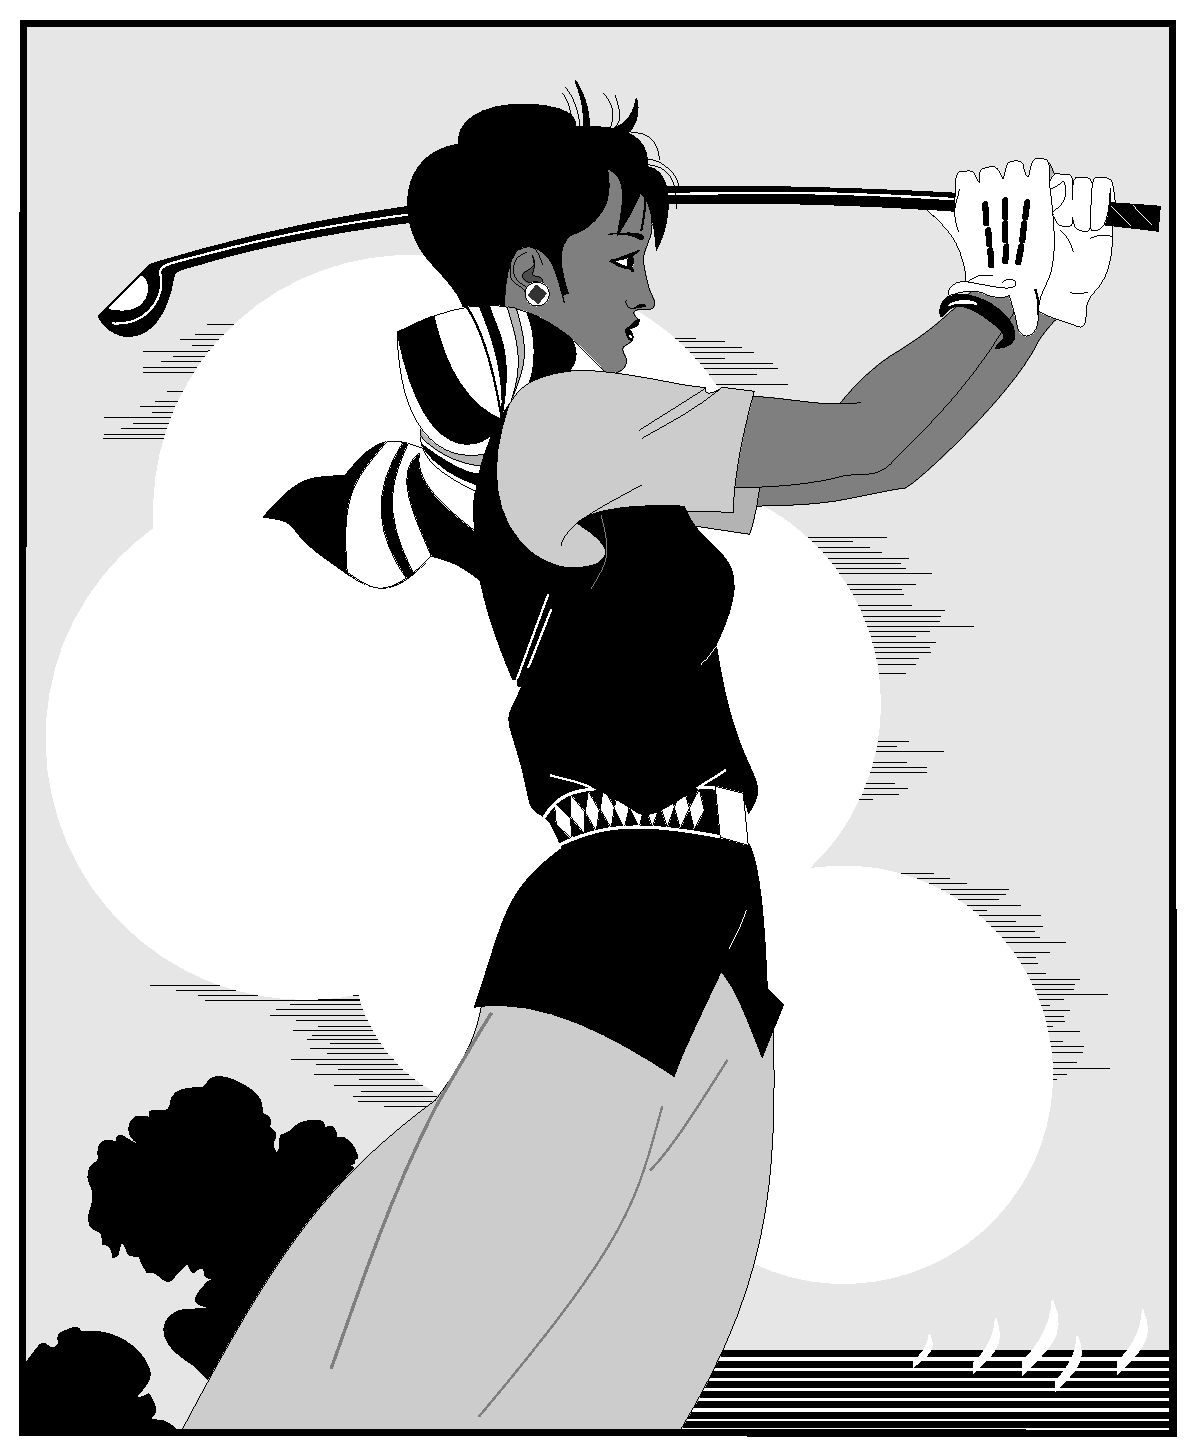
\includegraphics[width = 0.4\textwidth]{golfer}
% \bicaption[golfer1]{}{注意图中文字尽量用五号字
% }{Fig.$\!$}{The person playing golf}
% \end{figure}
% \end{latex}
% 单张单图题的格式如下,
% \begin{latex}
% \begin{figure}[h]
% \centering
% 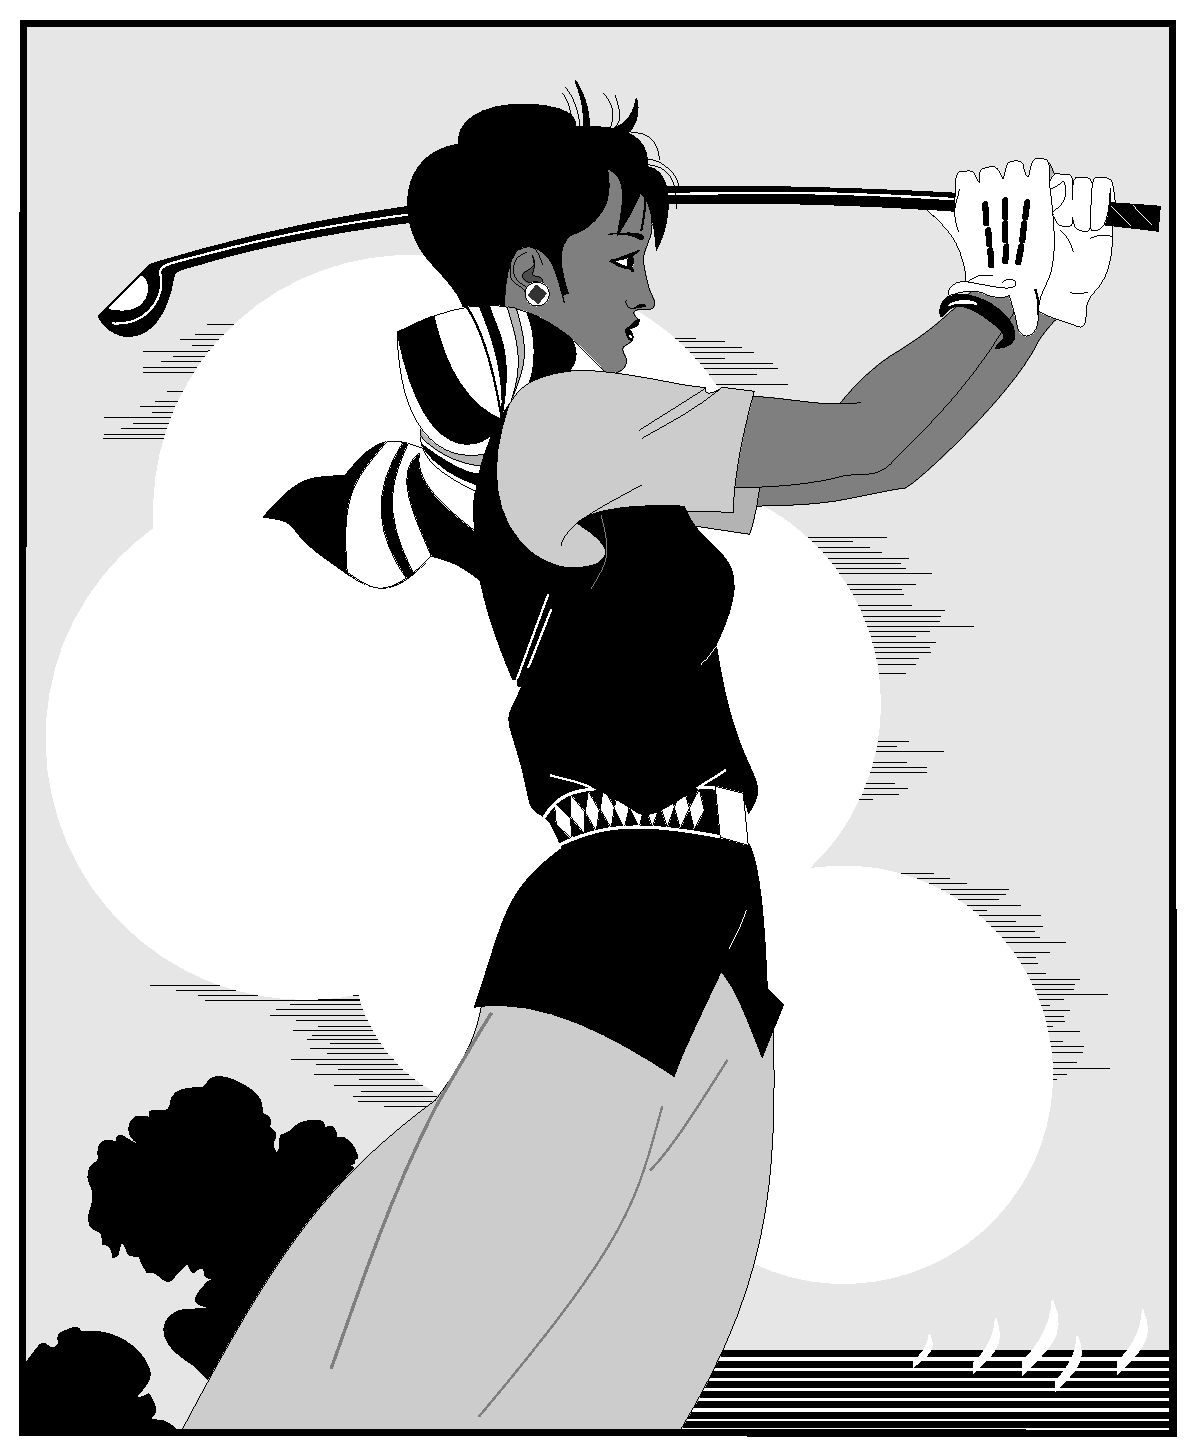
\includegraphics[width = 0.4\textwidth]{golfer}
% \caption{注意图中文字字号尽量用五号字}
% \end{figure}
% \end{latex}
% 并排图例。
% \begin{latex}
% \begin{figure}[htbp]
% \centering
% \begin{minipage}{0.4\textwidth}
% \centering
% 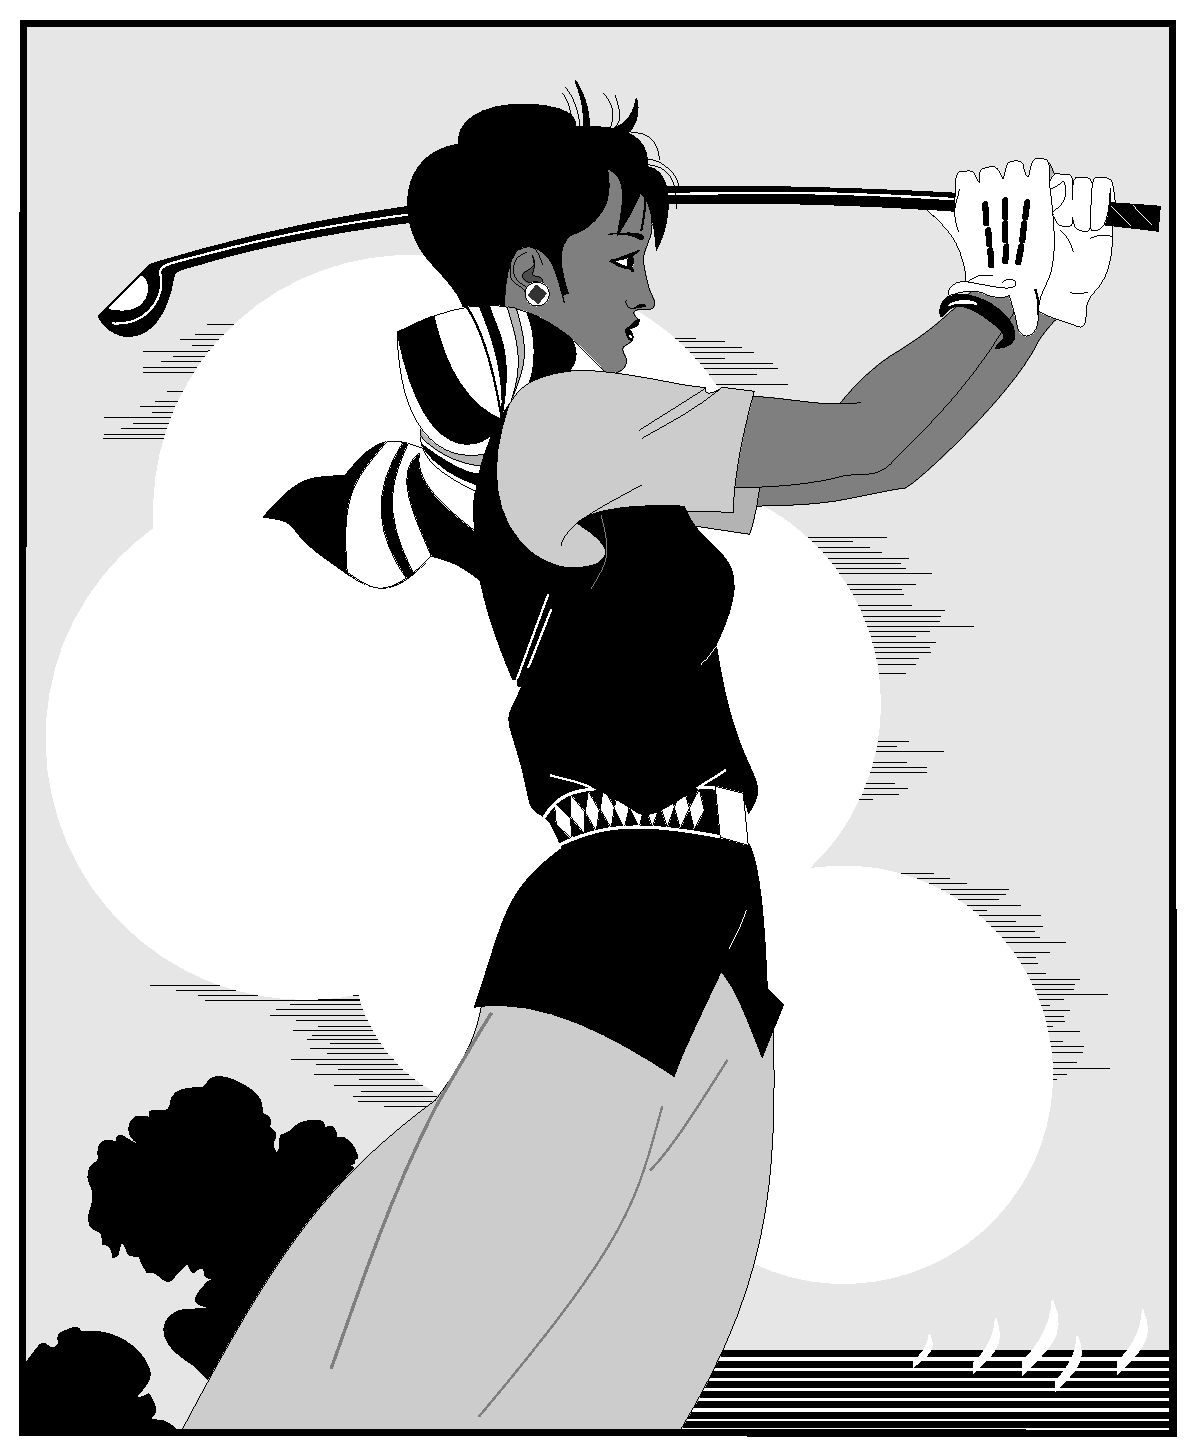
\includegraphics[width=\textwidth]{golfer}
% \bicaption[golfer2]{}{打高尔夫球的人}{Fig.$\!$}{The person playing golf}
% \end{minipage}
% \begin{minipage}{0.4\textwidth}
% \centering
% 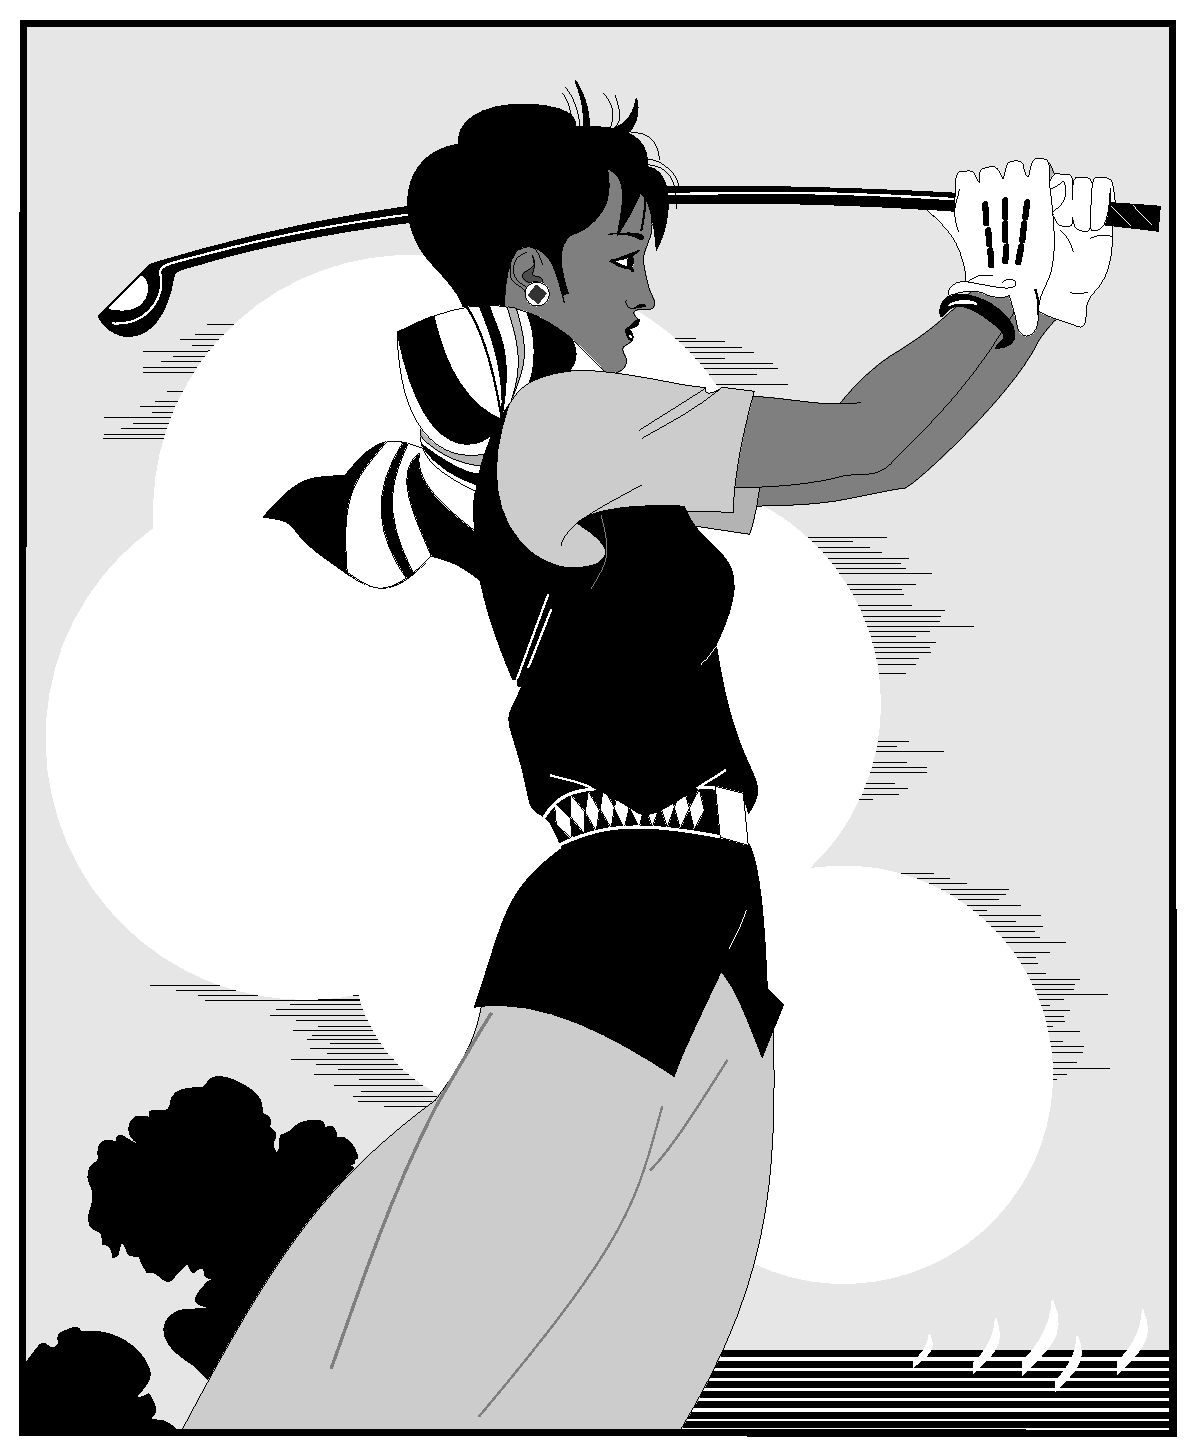
\includegraphics[width=\textwidth]{golfer}
% \bicaption[golfer3]{}{打高尔夫球的人}{Fig.$\!$}{The person playing golf}
% \end{minipage}
% \end{figure}
% \end{latex}
% 子图图例。
% \begin{latex}
% \begin{figure}[htbp]
% \centering
% \subfigure{\label{golfer41}}\addtocounter{subfigure}{-2}
% \subfigure[The person playing golf]{\subfigure[打高尔夫球的人~1]{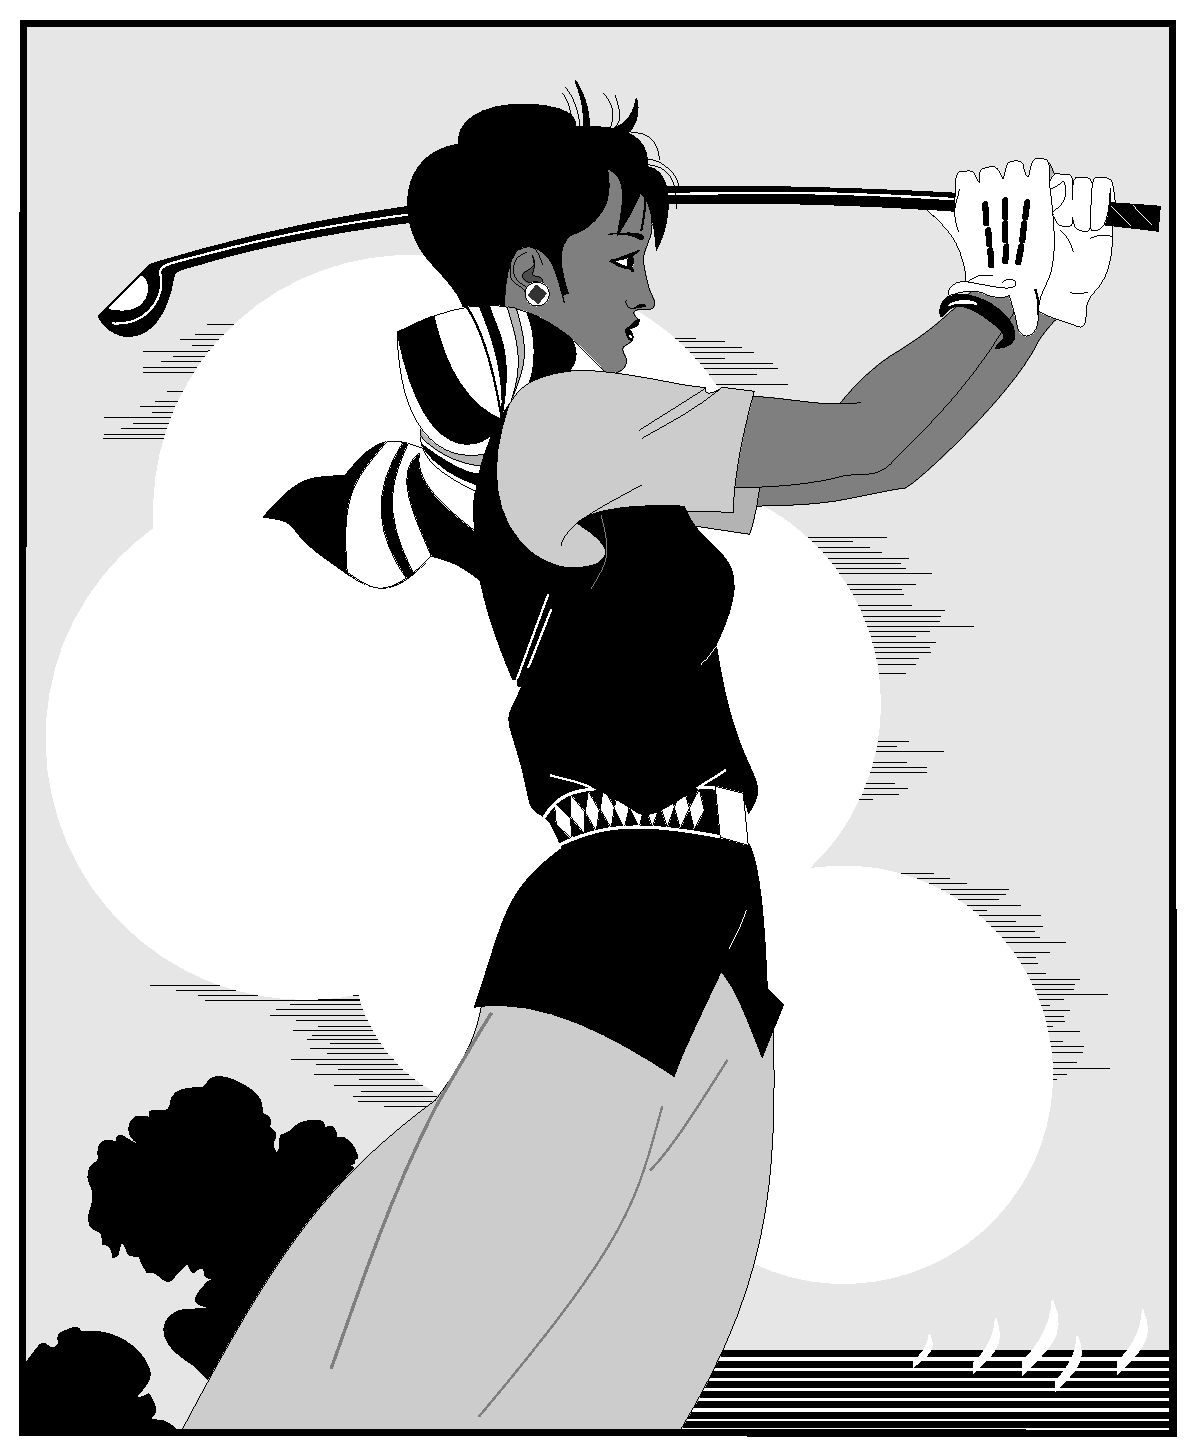
\includegraphics[width=0.4\textwidth]{golfer}}}
% \subfigure{\label{golfer42}}\addtocounter{subfigure}{-2}
% \subfigure[The person playing golf]{\subfigure[打高尔夫球的人~2]{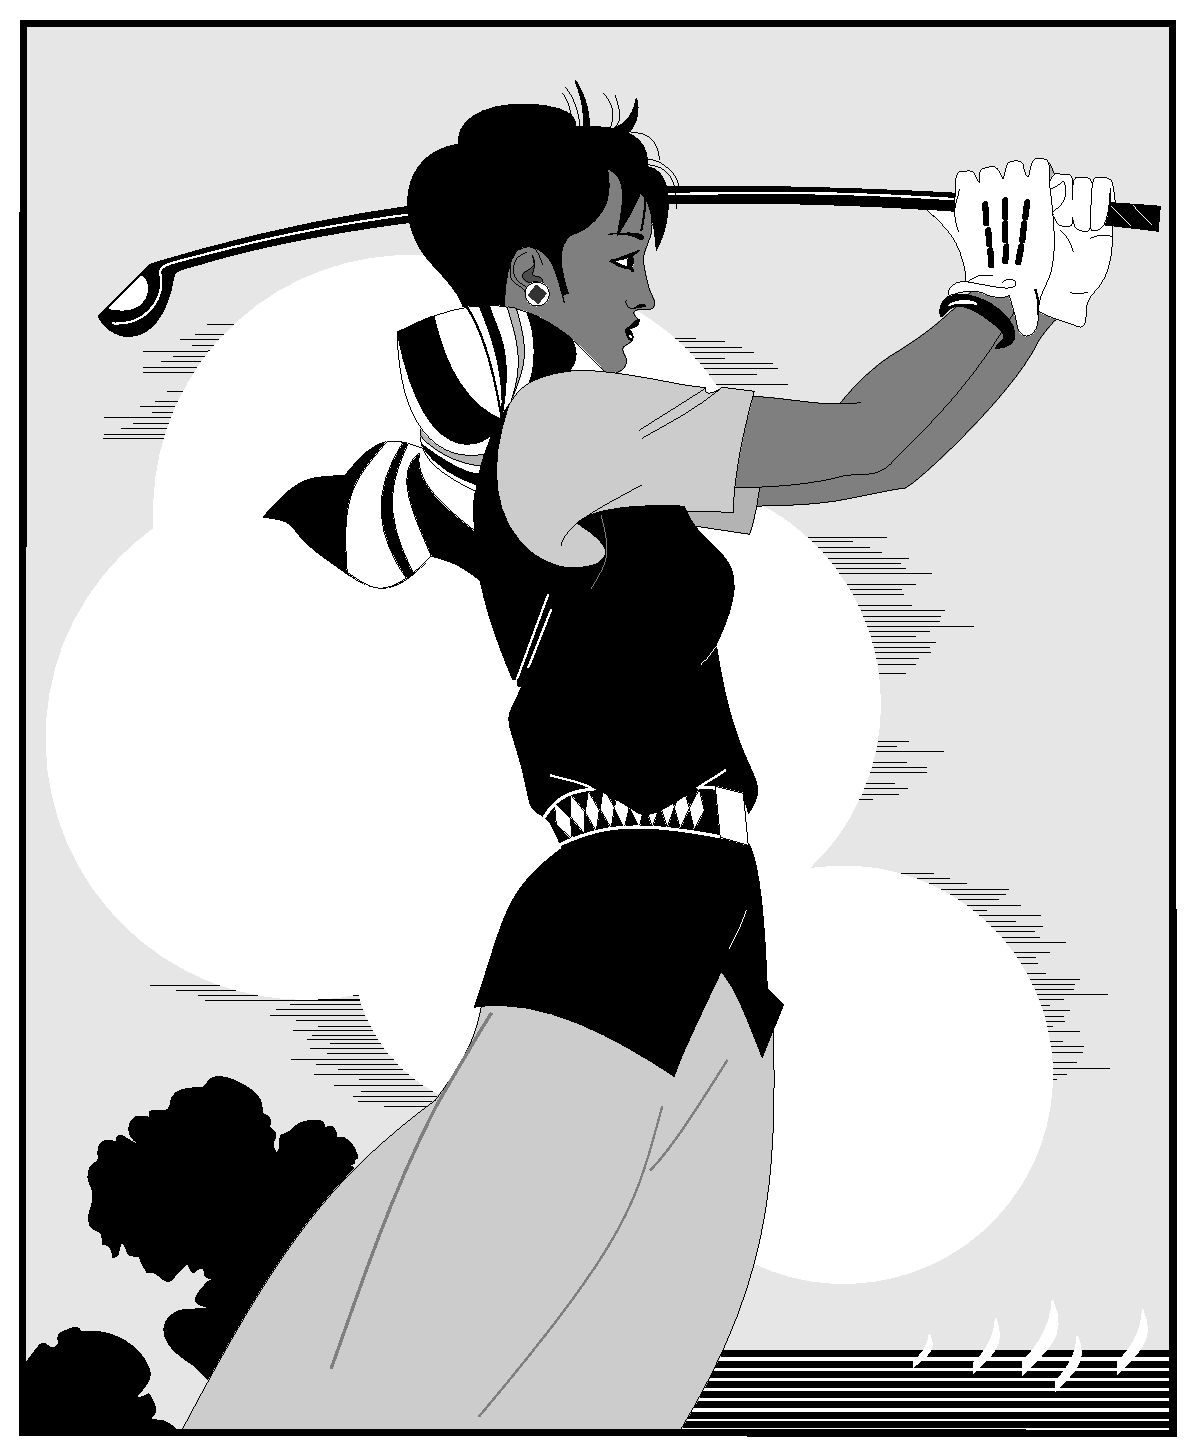
\includegraphics[width=0.4\textwidth]{golfer}}}
% \bicaption[golfer4]{}{打高尔夫球的人}{Fig.$\!$}{The person playing golf}
% \end{figure}
% \end{latex}
% 表格示例,表格中的字体是可以自行调整的。
% \begin{latex}
% \begin{table}[htbp]
% \bicaption[table1]{}{符合研究生院绘图规范的表格}{Table$\!$}{Table in agreement of the standard from graduate school}
% \vspace{0.5em}\centering\wuhao
% \begin{tabular}{ccccc}
% \toprule[1.5pt]
% $D$(in) & $P_u$(lbs) & $u_u$(in) & $\beta$ & $G_f$(psi.in)\\
% \midrule[1pt]
%  5 & 269.8 & 0.000674 & 1.79 & 0.04089\\
% 10 & 421.0 & 0.001035 & 3.59 & 0.04089\\
% 20 & 640.2 & 0.001565 & 7.18 & 0.04089\\
% \bottomrule[1.5pt]
% \end{tabular}
% \end{table}
% \end{latex}
% 因为长表格不是浮动体,不会自动调整位置、也不会自动调整字体大小,一切都要手动设
% 置。特别繁琐。
% \begin{latex}
% \ltfontsize{\dawu[1.667]} %设置表格内字体行间距
% \dawu[1.667]\begin{longtable}{ccc} % 注意此处设置的是表格线距离
% \longbionenumcaption{}{{\wuhao 中国省级行政单位一览 %此处要添加字体设置
% }\label{table2}}{Table$\!$}{}{{\wuhao Overview of the provincial administrative
% unit of China}}{-0.5em}{3.15bp}\\ %注意后两个参数分别是中英标题间距、标题和表格的间距。
% %\caption{\wuhao 中国省级行政单位一览}\\[1em] %注意此处是标题和表格间距,这行
% %是单语标题
% \toprule[1.5pt] 名称 & 简称 & 省会或首府  \\ \midrule[1pt]
% \endfirsthead
% \multicolumn{3}{r}{表~\thetable(续表)}\vspace{0.5em}\\
% \toprule[1.5pt] 名称 & 简称 & 省会或首府  \\ \midrule[1pt]
% \endhead
% \bottomrule[1.5pt]
% \endfoot
% 北京市 & 京 & 北京\\
% 天津市 & 津 & 天津\\
% 河北省 & 冀 & 石家庄市\\
% 山西省 & 晋 & 太原市\\
% 内蒙古自治区 & 蒙 & 呼和浩特市\\
% 辽宁省 & 辽 & 沈阳市\\
% 吉林省 & 吉 & 长春市\\
% 黑龙江省 & 黑 & 哈尔滨市\\
% 上海市 & 沪/申 & 上海\\
% 江苏省 & 苏 & 南京市\\
% 浙江省 & 浙 & 杭州市\\
% 安徽省 & 皖 & 合肥市\\
% 福建省 & 闽 & 福州市\\
% 江西省 & 赣 & 南昌市\\
% 山东省 & 鲁 & 济南市\\
% 河南省 & 豫 & 郑州市\\
% 湖北省 & 鄂 & 武汉市\\
% 湖南省 & 湘 & 长沙市\\
% 广东省 & 粤 & 广州市\\
% 广西壮族自治区 & 桂 & 南宁市\\
% 海南省 & 琼 & 海口市\\
% 重庆市 & 渝 & 重庆\\
% 四川省 & 川/蜀 & 成都市\\
% 贵州省 & 黔/贵 & 贵阳市\\
% 云南省 & 云/滇 & 昆明市\\
% 西藏自治区 & 藏 & 拉萨市\\
% 陕西省 & 陕/秦 & 西安市\\
% 甘肃省 & 甘/陇 & 兰州市\\
% 青海省 & 青 & 西宁市\\
% 宁夏回族自治区 & 宁 & 银川市\\
% 新疆维吾尔自治区 & 新 & 乌鲁木齐市\\
% 香港特别行政区 & 港 & 香港\\
% 澳门特别行政区 & 澳 & 澳门\\
% 台湾省 & 台 & 台北市\\
% \end{longtable}\normalsize %注意这里要恢复正常字体
% \end{latex}
% \subsubsection{公式}
% 公式不做介绍,与正常用法一致。
% \subsubsection{数学环境}
% \label{sec:math}
% \hithesis\ 定义了常用的数学环境:
%
% \begin{center}
% \begin{tabular}{*{7}{l}}\toprule
%   axiom & theorem & definition & proposition & lemma & conjecture &\\
%   公理 & 定理 & 定义 & 命题 & 引理 & 猜想 &\\\midrule
%   proof & corollary & example & exercise & assumption & remark & problem \\
%   证明 & 推论 & 例子& 练习 & 假设 & 注释 & 问题\\\bottomrule
% \end{tabular}
% \end{center}
%
% 比如:
% \begin{latex}
% \begin{definition}
%   道千乘之国,敬事而信,节用而爱人,使民以时。
% \end{definition}
% \end{latex}
% 产生(自动编号):
% \medskip
%
% \noindent\framebox[\linewidth][l]{{\heiti 定义~1.1~~~} % {道千乘之国,敬事而信,节用而爱人,使民以时。}}
%
% \smallskip
% 列举出来的数学环境毕竟是有限的,如果想用\emph{胡说}这样的数学环境,那么可以定义:
% \begin{latex}
% \newtheorem{nonsense}{胡说}[chapter]
% \end{latex}
%
% 然后这样使用:
% \begin{latex}
% \begin{nonsense}
%   契丹武士要来中原夺武林秘笈。—— 慕容博
% \end{nonsense}
% \end{latex}
% 产生(自动编号):
%
% \medskip
% \noindent\framebox[\linewidth][l]{{\heiti 胡说~1.1~~~} % {契丹武士要来中原夺武林秘笈。—— 慕容博}}
% \subsubsection{算法}
% 我工算法不在规范中要求且一千个评审老师有一千个算法格式喜好。详见
% \href{https://github.com/PlutoThesis/PlutoThesis#%E6%B2%A1%E6%9C%89%E6%98%8E%E7%A1%AE%E8%A6%81%E6%B1%82%E7%9A%84%E6%A0%BC%E5%BC%8F}{PlutoThesis}
% 中的各个实验室算法喜好举例。在此多说无益。
% \subsubsection{引用参考文献}
% \DescribeMacro{\inlinecite}
% 学校要求的参考文献引用有两种模式:(1)上标模式。比如``同样的工作有很
% 多$^{[1,2]}$\ldots''。(2)正文模式。比如``文[3] 中详细说明了\ldots''。其中上标
% 模式使用远比正文模式频繁,所以为了符合使用习惯,上标模式仍然用常规
% 的 \cs{cite}\marg{key},而 \cs{inlinecite}\marg{key} 则用来生成正文模式。
%
% 关于参考文献模板推荐使用 \BibTeX,关于中文参考文献需要额外增加一个 Entry:
% \texttt{lang},将其设置为 \texttt{zh} 用来指示此参考文献为中文,以
% 便 \file{hithesis.bst} 处理。如:
% \begin{latex}
% @INPROCEEDINGS{cnproceed,
%   author    = {王重阳 and 黄药师 and 欧阳峰 and 洪七公 and 段皇帝},
%   title     = {武林高手从入门到精通},
%   booktitle = {第~$N$~次华山论剑},
%   year      = 2006,
%   address   = {西安, 中国},
%   month     = sep,
%   lang      = "zh",
% }
%
% @ARTICLE{cnarticle,
%   AUTHOR  = "贾宝玉 and 林黛玉 and 薛宝钗 and 贾探春",
%   TITLE   = "论刘姥姥食量大如牛之现实意义",
%   JOURNAL = "红楼梦杂谈",
%   PAGES   = "260--266",
%   VOLUME  = "224",
%   YEAR    = "1800",
%   LANG    = "zh",
% }
% \end{latex}
%
% 注意如果不需要引用参考文献,请删除 \file{main.tex} 中 \cs{bibliography} 开头的两行,
% 以避免可能的编译错误。
%
% \subsubsection{列表环境}
% \DescribeEnv{itemize}
% \DescribeEnv{enumerate}
% \DescribeEnv{description}
% 为了适合中文习惯,模板将这三个常用的列表环境用 \pkg{enumitem} 进行了纵向间距压
% 缩。一方面清除了多余空间,另一方面用户可以自己指定列表环境的样式(如标签符号,
% 缩进等)。细节请参看 \pkg{enumitem} 文档,此处不再赘述。
% \subsection{后文}
%
% \subsubsection{结论}
% \DescribeEnv{conclusion}
% 结论之后为后文内容。
% \begin{latex}
% \begin{conclusions}
%
% 学位论文的结论作为论文正文的最后一章单独排写,但不加章标题序号。
%
% 结论应是作者在学位论文研究过程中所取得的创新性成果的概要总结,不能与摘要混为一
% 谈。博士学位论文结论应包括论文的主要结果、创新点、展望三部分,在结论中应概括论
% 文的核心观点,明确、客观地指出本研究内容的创新性成果(含新见解、新观点、方法创
% 新、技术创新、理论创新),并指出今后进一步在本研究方向进行研究工作的展望与设想
% 。对所取得的创新性成果应注意从定性和定量两方面给出科学、准确的评价,分(1)、
% (2)、(3)…条列出,宜用“提出了”、“建立了”等词叙述。
%
% \end{conclusions}
% \end{latex}
%
% \subsubsection{参考文献}
% 在后文中的参考文献是自动生成的,不需要用户干预,具体命令在\file{main.tex}中有
% 示例。
%
% \subsubsection{附录}
% \DescribeEnv{appendix}
% 所有的附录都插到这里来。因为附录会更改默认的 chapter 属性,而后面的{\heiti 个人简
%   历}又需要恢复,所以实现为环境可以保证全局的属性不受影响。
% \begin{latex}
% \begin{appendix}
% % -*-coding: utf-8 -*-
%%%%%%%%%%%%%%%%%%%%%%%%%%%%%%%%%%%%%%%%%%%%%%%%%%%%%%%%%
\chapter{带章节的附录}[Full Appendix]%
完整的附录内容,包含章节,公式,图表等

%%%%%%%%%%%%%%%%%%%%%%%%%%%%%%%%%%%%%%%%%%%%%%%%%%%%%%%%%
\section{附录节的内容}[Section in Appendix]
这是附录的节的内容

附录中图的示例:
\begin{figure}[htbp]
\centering
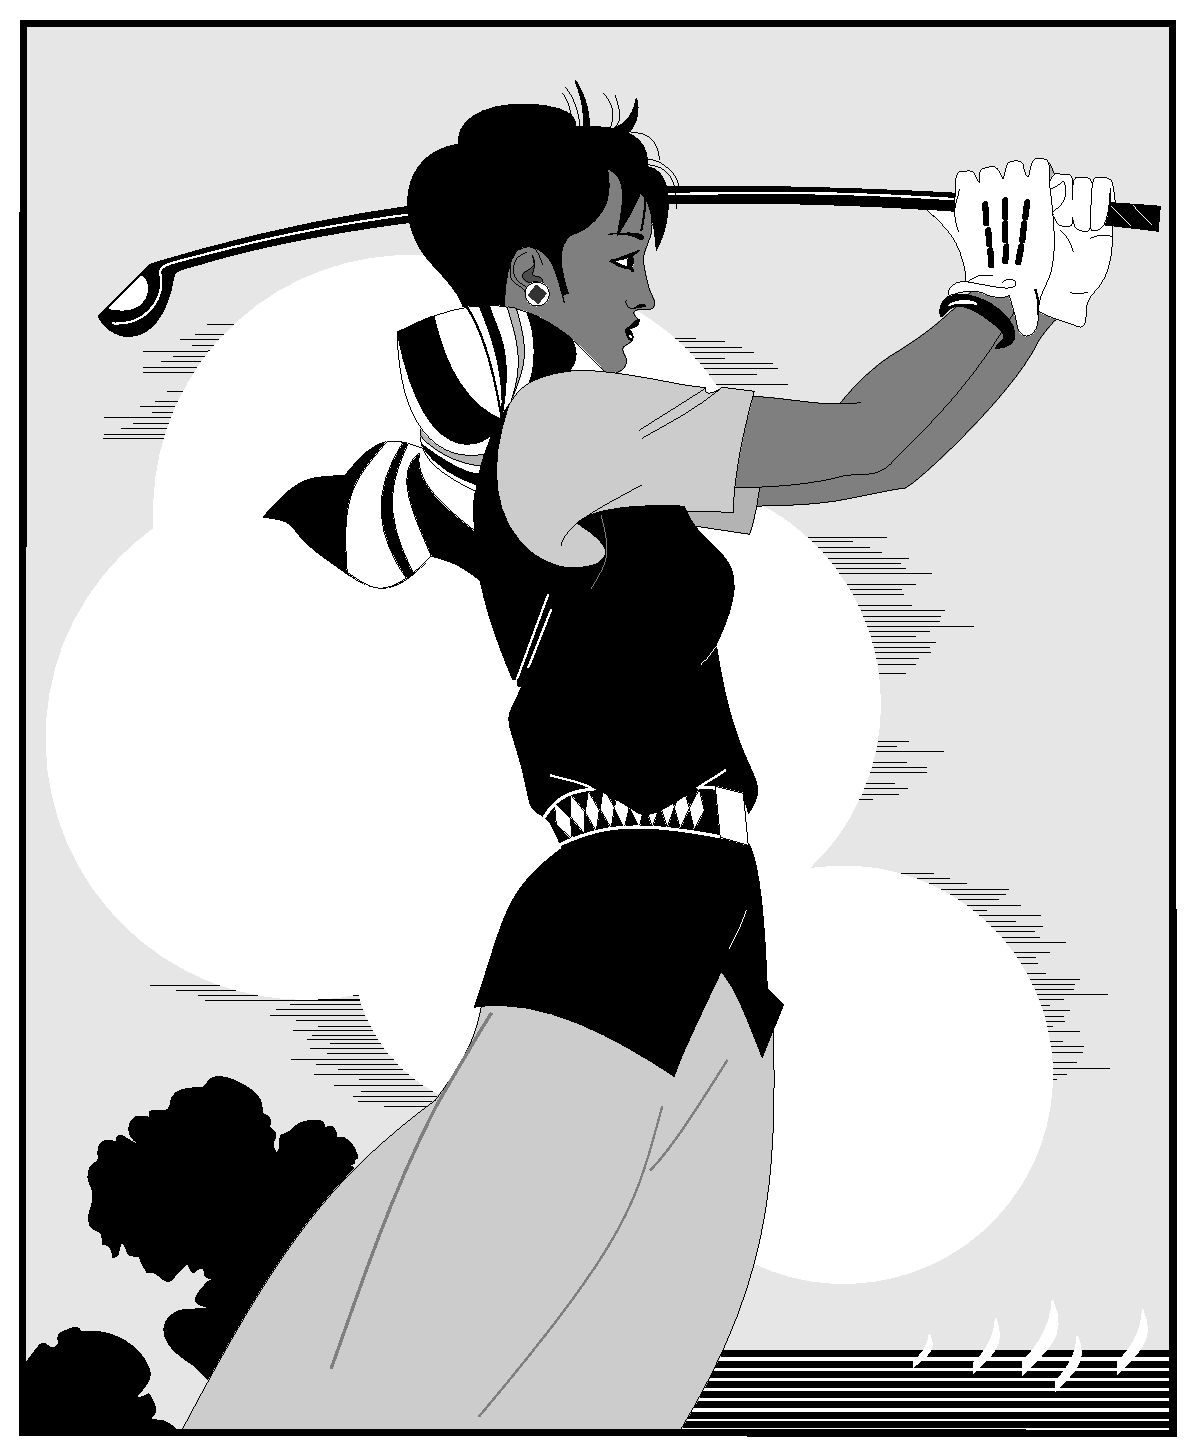
\includegraphics[width = 0.4\textwidth]{golfer}
%\bicaption[golfer5]{}{\xiaosi[0]打高尔夫球的人}{Fig.$\!$}{The person playing golf}\vspace{-1em}
\caption{\xiaosi[0]打高尔夫球的人}
\end{figure}

附录中公式的示例:
\begin{align}
a & = b \times c \\
E & = m c^2
\label{eq}
\end{align}

\chapter{这个星球上最好的免费Linux软件列表}[List of the Best Linux Software in our Planet]
\section{系统}

\href{http://fvwm.org/}{FVWM 自从上世纪诞生以来,此星球最强大的窗口管理器。}
推荐基于FVWM的桌面设计hifvwm:\href{https://github.com/dustincys/hifvwm}{https://github.com/dustincys/hifvwm}。

\subsection{hifvwm的优点}

\begin{enumerate}
	\item 即使打开上百个窗口也不会“蒙圈”。计算机性能越来越强大,窗口任务的管理必须要升级到打怪兽级别。
	\item 自动同步Bing搜索主页的壁纸。每次电脑开机,午夜零点自动更新,用户
		也可以手动更新,从此审美再也不疲劳。
	\item 切换窗口自动聚焦到最上面的窗口。使用键盘快捷键切换窗口时候,减少
		操作过程,自动聚焦到目标窗口。这一特性是虚拟窗口必须的人性化设
		计。
	\item 类似window右下角的功能的最小化窗口来显示桌面的功能此处类似
		win7/win10,实现在一个桌面之内操作多个任务。
	\item 任务栏结合标题栏。采用任务栏和标题栏结合,节省空间。
	\item 同类窗口切换。可以在同类窗口之内类似alt-tab的方式切换。
	\item ……
\end{enumerate}

\section{其他}

\href{https://github.com/goldendict/goldendict}{goldendict 星球最强大的桌面字典。}

\href{https://github.com/yarrick/iodine}{iodine,“HIT-WLAN + 锐捷”时代的福音。}

\href{http://www.aircrack-ng.org/}{aircrack,Wifi“安全性评估”工具。}

\href{https://www.ledger-cli.org/}{ledger,前“金融区块链”时代最好的复式记账系统。}

\href{https://orgmode.org/}{orgmode,最强大的笔记系统,从来没有之一。}

\href{https://www.jianguoyun.com/}{坚果云,国内一款支持WebDav的云盘系统,国内真正的云盘没有之一。}

\href{http://www.mutt.org/}{mutt, ``All mail clients suck. This one just sucks less.''}

\section{vim}
实现中英文每一句一行,以及实现每一句折叠断行的简单正则式,tex源码更加乖乖。
\begin{lstlisting}
vnoremap <leader>fae J:s/[.!?]\zs\s\+/\="\r".matchstr(getline('.'), '^\s*')/g<CR>
vnoremap <leader>fac J:s/[。!?]/\=submatch(0)."\n".matchstr(getline('.'), '^\s*')/g<CR>
vnoremap <leader>fle :!fmt -80 -s<CR>
\end{lstlisting}

% \end{appendix}
% \end{latex}
%
% \subsubsection{所发表文章}
% \DescribeEnv{publication}
% 虽然在\PGR\UGR\ 中都没有明确规定此处的格式,但按照旧模板PlutoThesis,此处格式
% 非常复杂。此处仍然使用旧模板中的设置方法。
% \begin{latex}
% \begin{publication}
% \noindent\textbf{(一)发表的学术论文}
% \begin{publist}
% \item	XXX,XXX. Static Oxidation Model of Al-Mg/C Dissipation Thermal Protection Materials[J]. Rare Metal Materials and Engineering, 2010, 39(Suppl. 1): 520-524.(SCI~收录,IDS号为~669JS,IF=0.16)
% \item XXX,XXX. 精密超声振动切削单晶铜的计算机仿真研究[J]. 系统仿真学报,2007,19(4):738-741,753.(EI~收录号:20071310514841)
% \item XXX,XXX. 局部多孔质气体静压轴向轴承静态特性的数值求解[J]. 摩擦学学报,2007(1):68-72.(EI~收录号:20071510544816)
% \item XXX,XXX. 硬脆光学晶体材料超精密切削理论研究综述[J]. 机械工程学报,2003,39(8):15-22.(EI~收录号:2004088028875)
% \item XXX,XXX. 基于遗传算法的超精密切削加工表面粗糙度预测模型的参数辨识以及切削参数优化[J]. 机械工程学报,2005,41(11):158-162.(EI~收录号:2006039650087)
% \item XXX,XXX. Discrete Sliding Mode Cintrok with Fuzzy Adaptive Reaching Law on 6-PEES Parallel Robot[C]. Intelligent System Design and Applications, Jinan, 2006: 649-652.(EI~收录号:20073210746529)
% \end{publist}
%
% \noindent\textbf{(二)申请及已获得的专利(无专利时此项不必列出)}
% \begin{publist}
% \item XXX,XXX. 一种温热外敷药制备方案:中国,88105607.3[P]. 1989-07-26.
% \end{publist}
%
% \noindent\textbf{(三)参与的科研项目及获奖情况}
% \begin{publist}
% \item	XXX,XXX. XX~气体静压轴承技术研究, XX~省自然科学基金项目.课题编号:XXXX.
% \item XXX,XXX. XX~静载下预应力混凝土房屋结构设计统一理论. 黑江省科学技术二等奖, 2007.
% \end{publist}
% %\vfill
% %\hangafter=1\hangindent=2em\noindent
% %\setlength{\parindent}{2em}
% \end{publication}
% \end{latex}
%
% \subsubsection{索引}
% \DescribeEnv{ceindex}
% 我工要求中英文双语索引。后文中的自动索引实际上不需要用户干预。
%\begin{latex}
% \begin{ceindex}
%   %如果想要手动加索引,注释掉以下这一样,用wordlist环境
% \printsubindex*
% \end{ceindex}
%\end{latex}
% 手工添加索引的方法不推荐,模板中将去除该功能。
% \subsubsection{授权}
% \DescribeMacro{\authorization}
% 授权页中的签名和日期是需要手写,不需要人工干预。具体示例在\file{main.tex}中。
%\begin{latex}
% \authorization %授权
% %\authorization[saomiao.pdf] %添加扫描页的命令,与上互斥
%\end{latex}
%
% \subsubsection{致谢声明}
% \DescribeEnv{acknowledgement}
% 把致谢做成一个环境更好一些,直接往里面写感谢的话就可以啦!
%
% \begin{latex}
% \begin{acknowledgement}
%   …
%   感谢\hit\LaTeX\ 论文模板\hithesis\ !
% \end{acknowledgement}
% \end{latex}
%
%
% \subsubsection{简历}
% \DescribeEnv{resume}
% 个人简历。
% 实际上,致谢和个人简历是自由发挥的地区,字体,文体,格式,内容,完全自己决定。
% \begin{latex}
% \begin{resume}
% XXXX~年~XX~月~XX~日出生于~XXXX。
%
% XXXX~年~XX~月考入~XX~大学~XX~院(系)XX~专业,XXXX~年~XX~月本科毕业并获得~XX~学学士学位。
%
% XXXX~年~XX~月------XXXX~年~XX~月在~XX~大学~XX~院(系)XX~学科学习并获得~XX~学硕士学位。
%
% XXXX~年~XX~月------XXXX~年~XX~月在~XX~大学~XX~院(系)XX~学科学习并获得~XX~学博士学位。
%
% 获奖情况:如获三好学生、优秀团干部、X~奖学金等(不含科研学术获奖)。
%
% 工作经历:
% \end{resume}
% \end{latex}
%
% \subsection{其它}
% 模板的配置文件 \file{hithesis.cfg} 中定义了很多固定词汇,一般无须修改。如果有特殊需求,
% 推荐在导言区使用 \cs{renewcommand}。
%
%
% \subsection{捐助}
% \changes{v1.0.1}{2017/08/27}{添加了捐助、矢量化本科论文模板的图片logo}
% 各位刀客和大侠如用的嗨,要解囊相助,请微信或支付宝参照图
% ~\ref{wct5}-\ref{zfb}~中提示操作(二维码被矢量化后之后去
% 除了头像等冗余无用的部分~)。
% \begin{figure}[h]
% \centering\includegraphics[width=0.5\textwidth]{wct5.eps}
% \caption{如果用的嗨,微信扫码捐助5元~~}
% \label{wct5}
% \end{figure}
% \begin{figure}[h]
% \centering\includegraphics[width=0.5\textwidth]{wct10.eps}
% \caption{如果用的非常嗨,微信扫码捐助10元~~}
% \label{wct10}
% \end{figure}
% \begin{figure}[h]
% \centering\includegraphics[width=0.5\textwidth]{wct1.eps}
% \caption{那个,看在熬夜写代码的份上,微信扫码捐助1元吧~~}
% \label{wct1}
% \end{figure}
% \begin{figure}[h]
% \centering\includegraphics[width=0.5\textwidth]{zfb.eps}
% \caption{支付宝不限额度}
% \label{zfb}
% \end{figure}
%
% \StopEventually{\PrintChanges\PrintIndex}
% \clearpage
%
% \section{实现细节}
%
% \subsection{基本信息}
%    \begin{macrocode}
%<cls>\NeedsTeXFormat{LaTeX2e}[1999/12/01]
%<cls>\ProvidesClass{hithesis}
%<cfg>\ProvidesFile{hithesis.cfg}
%<cls|cfg>[2018/12/05 2.0.6 Harbin Institute of Technology Thesis Template]
%    \end{macrocode}
%
% \subsection{定义选项}
% \label{sec:defoption}
%    \begin{macrocode}
%<*cls>
\RequirePackage{ifthen}
\RequirePackage{kvoptions}
\SetupKeyvalOptions{
  family=hit,
  prefix=hit@,
  setkeys=\kvsetkeys}
\newif\ifhit@bachelor
\newif\ifhit@master
\newif\ifhit@doctor
\define@key{hit}{type}{%
  \hit@bachelorfalse
  \hit@masterfalse
  \hit@doctorfalse
  \expandafter\csname hit@#1true\endcsname}
%    \end{macrocode}
%	定义stage项,区分开题、中期,默认false,为毕业论文,empty为空-去掉页眉 _added by t
%    \begin{macrocode}
\newif\ifhit@kaiti
\newif\ifhit@zhongqi
\define@key{hit}{stage}{%
  \hit@kaitifalse
  \hit@zhongqifalse
  \expandafter\csname hit@#1true\endcsname}
%    \end{macrocode}
%    设置版芯,由于窝工版芯歧义。
% \changes{v2.0.0}{2018/6/14}{此处添加geometry选项}
%    \begin{macrocode}
\newif\ifhit@geometrynewone
\newif\ifhit@geometrynewtwo
\define@key{hit}{newgeometry}{%
  \hit@geometrynewonefalse
  \hit@geometrynewtwofalse
  \expandafter\csname hit@geometrynew#1true\endcsname}
%    \end{macrocode}
% 目录中英文是否用 Arial 字体(默认关闭)。
%    \begin{macrocode}
\DeclareBoolOption[false]{arialtoc}
%    \end{macrocode}
% 章节标题中的英文是否用 Arial 字体(默认打开)。
%    \begin{macrocode}
\DeclareBoolOption[false]{arialtitle}
%    \end{macrocode}
% \changes{v1.0.3}{2017/08/29}{默认开启raggedbottom}
% \option{raggedbottom} 选项(默认开启)。如果不开启这个选项,会出现一页中尽量上
% 下对齐,段的间距大。如果开启,尽量使段间距保持一致,页面底部出现空白。
%    \begin{macrocode}
\DeclareBoolOption[true]{raggedbottom}
%    \end{macrocode}
% 在脚注标记中使用 \pkg{pifont} 的带圈数字(默认关闭)。
%    \begin{macrocode}
\DeclareBoolOption[false]{pifootnote}
%    \end{macrocode}
% 字体间距设置(默认关闭)。
%    \begin{macrocode}
\DeclareBoolOption[false]{glue}
%    \end{macrocode}
% 文科生四级目录设置(默认关闭)。
%    \begin{macrocode}
\DeclareBoolOption[false]{tocfour}
%    \end{macrocode}
% 目录中“目录”位置是否空行(默认开启)。
%    \begin{macrocode}
\DeclareBoolOption[true]{tocblank}
%    \end{macrocode}
% 章标题是否悬挂居中(默认开启)
%    \begin{macrocode}
\DeclareBoolOption[true]{chapterhang}
%    \end{macrocode}
% 是否是全日制学生(默认是)。
%    \begin{macrocode}
\DeclareBoolOption[true]{fulltime}
%    \end{macrocode}
% 是否有子标题(默认是)。
%    \begin{macrocode}
\DeclareBoolOption[false]{subtitle}
%    \end{macrocode}
% 是否开启debug模式(默认否)。如果开启,载入显示行号等的包,只为开发调试用。
%    \begin{macrocode}
\DeclareBoolOption[false]{debug}
%    \end{macrocode}
% \changes{v2.0.0}{2018/6/14}{此处删除newgeometry选项}
% 是否使用右开页(默认否)。
%    \begin{macrocode}
\DeclareBoolOption[false]{openright}
%    \end{macrocode}
% 图题和标题最后一行是否居中对其(默认是,非规范要求)。
% \changes{v1.0.6}{2017/10/25}{此处更改了选项的名称}
%    \begin{macrocode}
\DeclareBoolOption[false]{capcenterlast}
%    \end{macrocode}
% 子图图题和标题最后一行是否居中对其(默认是,非规范要求)。
% \changes{v1.0.6}{2017/10/25}{此处添加子图最后一行图题是否居中选项}
%    \begin{macrocode}
\DeclareBoolOption[false]{subcapcenterlast}
%    \end{macrocode}
% 中文目录中Abstract是否均为大写
% \changes{v1.0.13}{2018/4/5}{此处添加中文目录中Abstract是否均为大写选项}
%    \begin{macrocode}
\DeclareBoolOption[false]{absupper}
%    \end{macrocode}
%    此处添加控制本科论文的页码横线选项
% \changes{v1.0.15}{2018/06/05}{添加控制本科论文的页码横线选项}
%    \begin{macrocode}
\DeclareBoolOption[false]{bsmainpagenumberline}
\DeclareBoolOption[false]{bsfrontpagenumberline}
\DeclareBoolOption[true]{bsheadrule}
%    \end{macrocode}
%    数学字体是否使用新罗马
% \changes{v2.0.5}{2018/12/05}{添加数学字体开关}
%    \begin{macrocode}
\DeclareBoolOption[true]{newtxmath}
%    \end{macrocode}
%    此处应广大刀客要求添加一参考文献分割开关
% \changes{v2.0.3}{2018/10/08}{添加参考文献分割开关}
%    \begin{macrocode}
\DeclareBoolOption[false]{splitbibitem}
%    \end{macrocode}
% 声明字体选项。
%    \begin{macrocode}
\DeclareBoolOption[false]{customheadfancy}
%	添加customheadfancy项,可以用来自定义页眉,默认false,暂时无用  _added by t
\DeclareBoolOption[false]{noheader}
%	添加noheader项,true时可以用来去掉页眉(开题、中期报告老师可能不让留页眉),默认false,保留页眉  _added by t
\DeclareStringOption{fontset}
%    \end{macrocode}
% 将其余选项默认传递给 \pkg{ctexbook}。
%    \begin{macrocode}
\DeclareDefaultOption{\PassOptionsToClass{\CurrentOption}{ctexbook}}
%    \end{macrocode}
% 解析用户传递过来的选项,并加载 \pkg{ctexbook}。
%    \begin{macrocode}
\ProcessKeyvalOptions*
%    \end{macrocode}
% 使用 \XeTeX\ 引擎时,\pkg{fontspec} 宏包会被 \pkg{xeCJK} 自动调用。传递
% 给 \pkg{fontspec} 宏包 \option{no-math} 选项,避免部分数学符号字体自动调整
% 为 CMR。其他引擎下没有这个问题,这一行会被无视。
%    \begin{macrocode}
\PassOptionsToPackage{no-math}{fontspec}
%    \end{macrocode}
% 载入单双面打印设置,本、硕单面,博士双面。
%    \begin{macrocode}
\ifhit@bachelor
\PassOptionsToClass{oneside}{book}
\fi
\ifhit@master
\PassOptionsToClass{oneside}{book}
\fi
\ifhit@doctor
\PassOptionsToClass{twoside}{book}
\fi
%    \end{macrocode}
% \changes{v1.0.2}{2017/08/27}{添加了思源字体说明}
% 设置字体。由于宋体没有粗体,且我工模板的标题要求使用粗宋体,于是面临CTeX的经典
% 的伪粗体bug:“首次出现伪粗体字体之后的正常字体无法复制”。但如果使用自带宋体的
% 思源字体,那么不必使用伪粗体。模板只给出了新windows字体的思源字体设置,且思源
% 字体版本为Adobe版。
%    \begin{macrocode}
\ifthenelse%
{\equal{\hit@fontset}{}}%
{%
  \PassOptionsToPackage{AutoFakeBold=2}{xeCJK}
}%
{%
  \ifthenelse%
  {\equal{\hit@fontset}{siyuan}}%
  {\relax}%
  {%
    \PassOptionsToPackage{AutoFakeBold=2}{xeCJK}
  }%
  \PassOptionsToClass{fontset=\hit@fontset}{ctexbook}
}%
%    \end{macrocode}
% 使用 \pkg{ctexbook} 类,优于调用 \pkg{ctex} 宏包。
%    \begin{macrocode}
\LoadClass[a4paper,openany,UTF8,zihao=-4,scheme=plain]{ctexbook}
%    \end{macrocode}
% 用户至少要提供一个选项,指定论文类型。
%    \begin{macrocode}
\ifhit@bachelor\relax\else
  \ifhit@master\relax\else
    \ifhit@doctor\relax\else
        \ClassError{hithesis}%
                   {Please specify thesis type in option: \MessageBreak
                    type=[bachelor | master | doctor]}{}
      \fi
  \fi
\fi
%    \end{macrocode}
%
% \subsection{装载宏包}
% \label{sec:loadpackage}
%
% 引用的宏包和相应的定义。
%    \begin{macrocode}
\RequirePackage{etoolbox}
\RequirePackage{ifxetex}
\ifxetex
\else
        \ClassError{hithesis}%
                   {Please use: \MessageBreak
                    xelatex}{}
\fi
\RequirePackage{xparse}
%    \end{macrocode}
%
% \AmSTeX\ 宏包,用来排出更加漂亮的公式。
%    \begin{macrocode}
\RequirePackage{amsmath}
%    \end{macrocode}
% \pkg{newtx} 设置 Times New Roman,Helvetica。
%    \begin{macrocode}
\RequirePackage[defaultsups]{newtxtext}
%    \end{macrocode}
% 添加数学字体开关
%    \begin{macrocode}
\ifhit@newtxmath
\RequirePackage{newtxmath}
\fi
%    \end{macrocode}
% \pkg{newtx} 的 Mono 字体虽然很好看,但在论文中不常见。学校虽未要求 Mono 字体,
% 还是选择常见的 Courier 字体。由于比较新的实现 \TeX\ Gyre Cursor 会修
% 改\cs{bfdefault},导致中文加粗出问题,所以选用标准 \pkg{courier}。
%    \begin{macrocode}
\RequirePackage{courier}
%    \end{macrocode}
% 图形支持宏包。
%    \begin{macrocode}
\RequirePackage{graphicx}
%    \end{macrocode}
% \pkg{pdfpages} 宏包便于我们插入扫描后的授权页和声明页 PDF 文档。
%    \begin{macrocode}
\RequirePackage{pdfpages}
\includepdfset{fitpaper=true}
%    \end{macrocode}
% 更好的列表环境。
%    \begin{macrocode}
\RequirePackage{enumitem}       %使用enumitem宏包,改变列表项的格式
\RequirePackage{environ}
%    \end{macrocode}
% 禁止 \LaTeX 自动调整多余的页面底部空白,并保持脚注仍然在底部。
% 脚注按页编号。
%    \begin{macrocode}
\ifhit@raggedbottom
  \RequirePackage[bottom,perpage,hang]{footmisc}
  \raggedbottom
\else
  \RequirePackage[perpage,hang]{footmisc}
\fi
%    \end{macrocode}
% 脚注格式。
%    \begin{macrocode}
\ifhit@pifootnote
  \RequirePackage{pifont}
\fi
%    \end{macrocode}
% 利用 \pkg{CJKfntef} 实现汉字的下划线和盒子内两段对齐,并可以避免
% \cs{makebox}\oarg{width}\oarg{s} 可能产生的 underful boxes。
%    \begin{macrocode}
\RequirePackage{CJKfntef}
%    \end{macrocode}
% 定理类环境宏包,其中 \pkg{amsmath} 选项用来兼容 \AmSTeX\ 的宏包
%    \begin{macrocode}
\RequirePackage[amsmath,thmmarks,hyperref]{ntheorem}
%    \end{macrocode}
% 表格控制
%    \begin{macrocode}
\RequirePackage{longtable}
%    \end{macrocode}
% 使用三线表:\cs{toprule},\cs{midrule},\cs{bottomrule}。
%    \begin{macrocode}
\RequirePackage{booktabs}
%    \end{macrocode}
% 参考文献引用宏包。
%    \begin{macrocode}
\RequirePackage[sort&compress]{natbib}
%    \end{macrocode}
% 生成有书签的 pdf 及其开关,请结合 gbk2uni 避免书签乱码。
%    \begin{macrocode}
\RequirePackage{hyperref}
\hypersetup{%
  CJKbookmarks=true,
  linktoc=all,
  bookmarksnumbered=true,
  bookmarksopen=true,
  bookmarksopenlevel=1,
  breaklinks=true,
  colorlinks=false,
  plainpages=false,
  pdfborder=0 0 0}
%    \end{macrocode}
% 设置 url 样式,与上下文一致
%    \begin{macrocode}
\urlstyle{same}
%    \end{macrocode}
%
% \subsection{页面设置}
% \label{sec:layout}
% 本来这部分应该是最容易设置的,但根据我工\PGR\ 的3.8,3.4,3.2节的版芯矛盾,此处
% 设置两种版芯。
%    \begin{macrocode}
\ifhit@debug\RequirePackage[showframe]{geometry}\else\RequirePackage{geometry}\fi
\geometry{%根据PlutoThesis 原版定义而来
  a4paper, % 210 * 297mm
  hcentering,
  ignoreall,
  nomarginpar,
}
%    \end{macrocode}
%    添加版芯设置选项
%    \changes{v2.0.0}{2018/6/14}{添加版芯设置选项}
%    \begin{macrocode}
\ifhit@geometrynewtwo%
	\geometry{
	  centering,
	  text={150true mm,236true mm},
	  left=30true mm,
	  head=5true mm,
	  headsep=2true mm,
	  footskip=0true mm,
	  foot=5.2true mm
	}
\else%
	\ifhit@geometrynewone%
		\geometry{
		  centering,
		  text={150true mm,240true mm},
		  left=30true mm,
		  head=5true mm,
		  headsep=0true mm,
		  footskip=0true mm,
		  foot=0true mm
		}
	\else%
		\geometry{%根据PlutoThesis 原版定义而来
			text={150true mm,224true mm},
			top=35.5true mm,
			left=30true mm,
			head=5true mm,
			headsep=2.5true mm,
			foot=8.5true mm
		}
	\fi%
\fi%
%    \end{macrocode}
%    载入显示行号的包。
% \changes{v1.0.9}{2018/01/07}{添加debug包}
%    \begin{macrocode}
\ifhit@debug%
\RequirePackage{layout}
\RequirePackage{layouts}
\RequirePackage{lineno}
\fi
%    \end{macrocode}
% 利用 \pkg{fancyhdr} 设置页眉页脚。
%    \begin{macrocode}
\RequirePackage{fancyhdr}
%    \end{macrocode}
% 其他包,表格、数学符号包
% \changes{v1.0.6}{2017/10/25}{此处添加子图最后一行图题是否居中选项}
%    \begin{macrocode}
\RequirePackage{tabularx}
\RequirePackage{varwidth}
%    \end{macrocode}
% 此处changepage环境用来控制索引页面的左右边距,规范中给出的示例的边距要大于正文。
% \changes{v1.0.10}{2018/02/19}{修改了索引的间距,使其更符合规范中的示例}
%    \begin{macrocode}
\RequirePackage{changepage}
\RequirePackage{multicol}
\RequirePackage{amssymb}
\RequirePackage[below]{placeins}%允许上一个section的浮动图形出现在下一个section的开始部分,还提供\FloatBarrier命令,使所有未处理的浮动图形立即被处理
\RequirePackage{flafter}       % 使得所有浮动体不能被放置在其浮动环境之前,以免浮动体在引述它的文本之前出现.
\RequirePackage{multirow}       %使用Multirow宏包,使得表格可以合并多个row格
\ifhit@subcapcenterlast
\PassOptionsToPackage{centerlast}{subfigure}
\fi
\RequirePackage{subfigure}%支持子图 %centerlast 设置最后一行是否居中
\RequirePackage[subfigure]{ccaption} %支持双语标题
%    \end{macrocode}
%    中英文索引包。
%    \begin{macrocode}
\RequirePackage[makeindex]{splitidx}
\newindex[]{china}
\newindex[]{english}
%</cls>
%    \end{macrocode}
%    我工要求的索引格式。
% \changes{v1.0.10}{2018/02/19}{修改了索引的间距,使其更符合规范中的示例}
%    \begin{macrocode}
%<*ist>
headings_flag 1
heading_prefix "\{\\vskip -\\baselineskip\\centering\\normalsize\\textbf\{"
heading_suffix "\}\\par\}\\nopagebreak\\wuhao\n"
delim_0 "\\hspace*{\\fill}"
delim_1 "\\hspace*{\\fill}"
%</ist>
%    \end{macrocode}
%    排版logo。
%    \begin{macrocode}
%<cls>\RequirePackage{xltxtra}
%    \end{macrocode}
%
% \subsection{主文档格式}
% \label{sec:mainbody}
%
% \subsubsection{Three matters}
% \begin{macro}{\cleardoublepage}
% 对于 \textsl{openright} 选项,必须保证章首页右开,且如果前章末页无内容须
% 清空其页眉页脚。
%    \begin{macrocode}
%<*cls>
\let\hit@cleardoublepage\cleardoublepage
\newcommand{\hit@clearemptydoublepage}{%
  \clearpage{\pagestyle{hit@empty}\hit@cleardoublepage}
}
\let\cleardoublepage\hit@clearemptydoublepage
%    \end{macrocode}
% \end{macro}
% \begin{macro}{\frontmatter}
% \begin{macro}{\mainmatter}
% \begin{macro}{\backmatter}
% 我们的单面和双面模式与常规的不太一样。
%    \begin{macrocode}
\renewcommand\frontmatter{%
  \ifhit@openright\cleardoublepage\else\clearpage\fi
  \@mainmatterfalse
  \pagenumbering{Roman}
  \pagestyle{hit@empty}
}

\renewcommand\mainmatter{%
  \ifhit@tocblank%
  \addtocontents{toc}{\vspace{\baselineskip}} %规范中并没有这一要求,此处不应该加
  \addtocontents{toe}{\vspace{\baselineskip}}
  \fi%
  \ifhit@openright\cleardoublepage\else\clearpage\fi
  \@mainmattertrue
  \pagenumbering{arabic}
  \pagestyle{hit@headings}
}

\renewcommand\backmatter{%
  \ifhit@openright\cleardoublepage\else\clearpage\fi
  \@mainmattertrue}
%</cls>
%    \end{macrocode}
% \end{macro}
% \end{macro}
% \end{macro}
%
% \subsubsection{字体}
% \label{sec:font}
% \begin{macro}{\normalsize}
% 根据我工规定,正文小四号 (12bp) 字,行距为固定值3--4mm。
%    \begin{macrocode}
%<*cls>
\renewcommand\normalsize{%
  \@setfontsize\normalsize{12bp}{\ifhit@glue 20.50398bp \@plus 2.83465bp \@minus 0bp\else 20.50398bp\fi}%
  \abovedisplayskip=8pt
  \abovedisplayshortskip=8pt
  \belowdisplayskip=\abovedisplayskip
  \belowdisplayshortskip=\abovedisplayshortskip}
%    \end{macrocode}
% \end{macro}
%
% WORD 中的字号对应该关系如下(1bp = 72.27/72 pt):
% \begin{center}
% \begin{tabular}{llll}
% \toprule
% 初号 & 42bp & 14.82mm & 42.1575pt \\
% 小初 & 36bp & 12.70mm & 36.135 pt \\
% 一号 & 26bp & 9.17mm & 26.0975pt \\
% 小一 & 24bp & 8.47mm & 24.09pt \\
% 二号 & 22bp & 7.76mm & 22.0825pt \\
% 小二 & 18bp & 6.35mm & 18.0675pt \\
% 三号 & 16bp & 5.64mm & 16.06pt \\
% 小三 & 15bp & 5.29mm & 15.05625pt \\
% 四号 & 14bp & 4.94mm & 14.0525pt \\
% 小四 & 12bp & 4.23mm & 12.045pt \\
% 五号 & 10.5bp & 3.70mm & 10.59375pt \\
% 小五 & 9bp & 3.18mm & 9.03375pt \\
% 六号 & 7.5bp & 2.56mm & \\
% 小六 & 6.5bp & 2.29mm & \\
% 七号 & 5.5bp & 1.94mm & \\
% 八号 & 5bp & 1.76mm & \\\bottomrule
% \end{tabular}
% \end{center}
%
% \begin{macro}{\hit@def@fontsize}
% 根据习惯定义字号。用法:\cs{hit@def@fontsize}\marg{字号名称}\marg{磅数}避免了
% 字号选择和行距的紧耦合。所有字号定义时为单倍行距,并提供选项指定行距倍数。
%    \begin{macrocode}
\def\hit@def@fontsize#1#2{%
  \expandafter\newcommand\csname #1\endcsname[1][1.3]{%
    \fontsize{#2}{##1\dimexpr #2}\selectfont}}
%    \end{macrocode}
% \end{macro}
%
% \begin{macro}{\chuhao}
% \begin{macro}{\xiaochu}
% \begin{macro}{\yihao}
% \begin{macro}{\xiaoyi}
% \begin{macro}{\erhao}
% \begin{macro}{\xiaoer}
% \begin{macro}{\sanhao}
% \begin{macro}{\xiaosan}
% \begin{macro}{\sihao}
% \begin{macro}{\banxiaosi}
% \begin{macro}{\xiaosi}
% \begin{macro}{\dawu}
% \begin{macro}{\wuhao}
% \begin{macro}{\xiaowu}
% \begin{macro}{\liuhao}
% \begin{macro}{\xiaoliu}
% \begin{macro}{\qihao}
% \begin{macro}{\bahao}
% 一组字号定义。
%    \begin{macrocode}
\hit@def@fontsize{chuhao}{42bp}
\hit@def@fontsize{xiaochu}{36bp}
\hit@def@fontsize{yihao}{26bp}
\hit@def@fontsize{xiaoyi}{24bp}
\hit@def@fontsize{erhao}{22bp}
\hit@def@fontsize{xiaoer}{18bp}
\hit@def@fontsize{sanhao}{16bp}
\hit@def@fontsize{xiaosan}{15bp}
\hit@def@fontsize{sihao}{14bp}
\hit@def@fontsize{banxiaosi}{13bp}
\hit@def@fontsize{xiaosi}{12bp}
\hit@def@fontsize{dawu}{11bp}
\hit@def@fontsize{wuhao}{10.5bp}
\hit@def@fontsize{xiaowu}{9bp}
\hit@def@fontsize{liuhao}{7.5bp}
\hit@def@fontsize{xiaoliu}{6.5bp}
\hit@def@fontsize{qihao}{5.5bp}
\hit@def@fontsize{bahao}{5bp}
%</cls>
%    \end{macrocode}
% \end{macro}
% \end{macro}
% \end{macro}
% \end{macro}
% \end{macro}
% \end{macro}
% \end{macro}
% \end{macro}
% \end{macro}
% \end{macro}
% \end{macro}
% \end{macro}
% \end{macro}
% \end{macro}
% \end{macro}
% \end{macro}
% \end{macro}
% \end{macro}
% \subsubsection{页眉页脚}
% \label{sec:headerfooter}
% \begin{macro}{\hit@empty}
% \begin{macro}{\hit@plain}
% \begin{macro}{\hit@headings}
% 定义三种页眉页脚格式:
% \begin{itemize}
% \item \texttt{hit@empty}:页眉页脚都没有
% \item \texttt{hit@plain}:只显示页脚的页码。\cs{chapter} 自动调用
% \cs{thispagestyle\{hit@plain\}}。
% \item \texttt{hit@headings}:页眉页脚同时显示
% \end{itemize}
%    \begin{macrocode}
%<*cls>
\let\hit@headrule\headrule
\fancypagestyle{hit@empty}{%
  \fancyhf{}
  \let\headrule\hit@headrule%
  \renewcommand{\headrulewidth}{0pt}
  \renewcommand{\footrulewidth}{0pt}
}
%    \end{macrocode}
%    此处根据本科生模板的多种版本,提供选项自定义页码、页眉样式。
%   \changes{v1.0.15}{2018/06/05}{添加控制本科论文的页码横线选项}
%   \changes{v1.0.15}{2018/06/05}{删除冗余的页面格式}
%    \begin{macrocode}
\fancypagestyle{hit@headings}{%
  \fancyhf{}
  \ifhit@doctor
	  \ifhit@kaiti	%页眉判断-开题 _added by t
	  \fancyhead[C]{\songti\xiaowu[0]\hit@cschoolname\hit@cdegree\hit@cthesisname\hit@stagestatus}
	  \else
	  \ifhit@zhongqi	%页眉判断-中期 _added by t
	  \fancyhead[C]{\songti\xiaowu[0]\hit@cschoolname\hit@cdegree\hit@cthesisname\hit@stagestatus}
	  \else
  \fancyhead[CO]{\songti\xiaowu[0]\leftmark}
  \fancyhead[CE]{\songti\xiaowu[0]\hit@cschoolname\hit@cdegree\hit@cthesisname}%
	  \fi
	  \fi
  \fi
  \ifhit@master
	  \ifhit@kaiti	%页眉判断-开题 _added by t
	  \fancyhead[C]{\songti\xiaowu[0]\hit@cschoolname\hit@cdegree\hit@cthesisname\hit@stagestatus}
	  \else
	  \ifhit@zhongqi	%页眉判断-中期 _added by t
	  \fancyhead[C]{\songti\xiaowu[0]\hit@cschoolname\hit@cdegree\hit@cthesisname\hit@stagestatus}
	  \else
  \fancyhead[C]{\songti\xiaowu[0]\hit@cschoolname\hit@cdegree\hit@cthesisname}
  	  \fi
  	  \fi
  \fi
  \ifhit@bachelor
	  \ifhit@kaiti	%页眉判断-开题 _added by t
	  \fancyhead[C]{\songti\xiaowu[0]\hit@cschoolname\hit@bachelor@cxuewei\hit@bachelor@cthesisname\hit@stagestatus}
	  \else
	  \ifhit@zhongqi	%页眉判断-中期 _added by t
	  \fancyhead[C]{\songti\xiaowu[0]\hit@cschoolname\hit@bachelor@cxuewei\hit@bachelor@cthesisname\hit@stagestatus}
	  \else
  \fancyhead[C]{\songti\xiaowu[0]\hit@cschoolname\hit@bachelor@cxuewei\hit@bachelor@cthesisname}%
      \fi
      \fi
  \fancyfoot[C]{\xiaowu\if@mainmatter\ifhit@bsmainpagenumberline-~\thepage~-\else\thepage\fi\else\ifhit@bsfrontpagenumberline-~\thepage~-\else\thepage\fi\fi}
	  \ifhit@noheader  %单独设置noheader项,可能会有老师要求在开题、中期报告没有页眉,此处优先级高于bsheadrule	_added by t
	  \fancyhf{}
	  \renewcommand{\headrulewidth}{0pt}
	  \else
	  \ifhit@bsheadrule
	  \renewcommand{\headrule}{
	  \vskip 1.190132pt
	  \hrule\@height2.276208pt\@width\headwidth
	  \vskip 0.75pt
	  \hrule\@height.75pt\@width\headwidth
	  }
	  \else
	  \renewcommand{\headrulewidth}{0pt}
	  \fi
	  \fi
     \else
	 \ifhit@noheader  %单独设置noheader项,可能会有老师要求在开题、中期报告没有页眉	_added by t
     \fancyhf{}
	 \renewcommand{\headrulewidth}{0pt}
	 \else
	 \renewcommand{\headrule}{
	 \vskip 1.190132pt
	 \hrule\@height2.276208pt\@width\headwidth
	 \vskip 0.75pt
	 \hrule\@height.75pt\@width\headwidth
	 }
	 \fi
	 \fi
  \fancyfoot[C]{\xiaowu-~\thepage~-}

  % 此处可能和word模板不一致
  % 页眉中小五汉字,0行距时,占用9bt,页眉高度为14pt, 所以以下数字之和要保持等于14pt-9bt=4.96634pt
  % 根据PlutoThesis模板中rule宽度定义为2.25, 0.75, 保持粗线和细线之间的间距为细线宽度。
  % 如果页眉是多行的情况,rule向下溢出
  \renewcommand{\footrulewidth}{0pt}
}
\AtBeginDocument{%此处解决页眉经典bug
  \pagestyle{hit@empty}
  \renewcommand{\chaptermark}[1]{\@mkboth{\CTEXthechapter\enspace#1}{}}}
%</cls>
%    \end{macrocode}
% \end{macro}
% \end{macro}
% \end{macro}
%
% \subsubsection{段落}
% \label{sec:paragraph}
%
% 全文首行缩进 2 字符,标点符号用全角
%    \begin{macrocode}
%<*cls>
\ctexset{%
  punct=quanjiao,
  space=auto,
  autoindent=true}
%    \end{macrocode}
% 利用 \pkg{enumitem} 命令调整默认列表环境间的距离,以符合中文习惯。
%    \begin{macrocode}
\setlist{nosep}
%</cls>
%    \end{macrocode}
% \subsubsection{脚注}
% \label{sec:footnote}
% 脚注符合中文习惯,数字带圈。
%    \begin{macrocode}
%<*cls>
\def\hit@textcircled#1{%
  \ifnum\value{#1} >9
    \ClassError{hithesis}%
      {Too many footnotes in this page.}{Keep footnote less than 10.}
  \fi
  \ifhit@pifootnote%
    \ding{\the\numexpr\value{#1}+171\relax}%
  \else%
    \textcircled{\xiaoliu\arabic{#1}}%
  \fi}
\renewcommand{\thefootnote}{\hit@textcircled{footnote}}
\renewcommand{\thempfootnote}{\hit@textcircled{mpfootnote}}
%    \end{macrocode}
% 定义脚注分割线,字号(宋体小五),以及悬挂缩进(1.5字符)。
%    \begin{macrocode}
\def\footnoterule{\vskip-3\p@\hrule\@width0.3\textwidth\@height0.4\p@\vskip2.6\p@}
\let\hit@footnotesize\footnotesize
\renewcommand\footnotesize{\hit@footnotesize\xiaowu[1.5]}
\footnotemargin1.5em\relax
%    \end{macrocode}
% \cs{@makefnmark} 默认是上标样式,而在脚注部分要求为正文大小。利用\cs{patchcmd}
% 动态调整 \cs{@makefnmark} 的定义。
%    \begin{macrocode}
\let\hit@makefnmark\@makefnmark
\def\hit@@makefnmark{\hbox{{\normalfont\@thefnmark}}}
\pretocmd{\@makefntext}{\let\@makefnmark\hit@@makefnmark}{}{}
\apptocmd{\@makefntext}{\let\@makefnmark\hit@makefnmark}{}{}
%</cls>
%    \end{macrocode}
% \subsubsection{数学相关}
% \label{sec:equation}
% 允许太长的公式断行、分页等。
%    \begin{macrocode}
%<*cls>
\allowdisplaybreaks[4]
\predisplaypenalty=0  %公式之前可以换页,公式出现在页面顶部
\postdisplaypenalty=0
\renewcommand\theequation{\ifnum \c@chapter>\z@ \thechapter-\fi\@arabic\c@equation}
%    \end{macrocode}
% \changes{v2.0.3}{2018/10/08}{设置公式前后随意断页}
% 公式距前后文的距离由 4 个参数控制,参见 \cs{normalsize} 的定义。
% 同时为了让 \pkg{amsmath} 的 \cs{tag*} 命令得到正确的格式,我们必须修改这些代
% 码。\cs{make@df@tag} 是定义 \cs{tag*} 和 \cs{tag} 内部命令的。
% \cs{make@df@tag@@} 处理 \cs{tag*},我们就改它!
% \begin{latex}
% \def\make@df@tag{\@ifstar\make@df@tag@@\make@df@tag@@@}
% \def\make@df@tag@@#1{%
%   \gdef\df@tag{\maketag@@@{#1}\def\@currentlabel{#1}}}
% \end{latex}
%    \begin{macrocode}
\def\make@df@tag{\@ifstar\hit@make@df@tag@@\make@df@tag@@@}
\def\hit@make@df@tag@@#1{\gdef\df@tag{\hit@maketag{#1}\def\@currentlabel{#1}}}
\iffalse
\ifhit@bachelor
  \def\hit@maketag#1{\maketag@@@{%
    (\ignorespaces\text{\equationname\hskip0.5em}#1\unskip\@@italiccorr)}}
  \def\tagform@#1{\maketag@@@{%
    (\ignorespaces\text{\equationname\hskip0.5em}#1\unskip\@@italiccorr)\equcaption{#1}}}
\fi
\fi
\def\hit@maketag#1{\maketag@@@{(\ignorespaces #1\unskip\@@italiccorr)}}
\def\tagform@#1{\maketag@@@{(\ignorespaces #1\unskip\@@italiccorr)\equcaption{#1}}}
%    \end{macrocode}
% 修改 \cs{tagform} 会影响 \cs{eqref}。
%    \begin{macrocode}
\renewcommand{\eqref}[1]{\textup{(\ref{#1})}}
%</cls>
%    \end{macrocode}
% 定理标题使用黑体,正文使用宋体,冒号隔开。
%    \begin{macrocode}
%<*cfg>
\theorembodyfont{\normalfont}
\theoremheaderfont{\normalfont\heiti}
\theoremsymbol{\ensuremath{\square}}
\newtheorem*{proof}{证明}
\theoremstyle{plain}
\theoremsymbol{}
%    \end{macrocode}
% 此处去除了冒号,(如果需要在加上这个冒号?),反正规范中没有。
% \changes{v2.0.2}{2018/06/28}{取出了定理冒号}
%    \begin{macrocode}
\theoremseparator{}
\newtheorem{assumption}{假设}[chapter]
\newtheorem{definition}{定义}[chapter]
\newtheorem{proposition}{命题}[chapter]
\newtheorem{lemma}{引理}[chapter]
\newtheorem{theorem}{定理}[chapter]
\newtheorem{axiom}{公理}[chapter]
\newtheorem{corollary}{推论}[chapter]
\newtheorem{exercise}{练习}[chapter]
\newtheorem{example}{例}[chapter]
\newtheorem{remark}{注释}[chapter]
\newtheorem{problem}{问题}[chapter]
\newtheorem{conjecture}{猜想}[chapter]
%</cfg>
%    \end{macrocode}
% \subsubsection{浮动对象以及表格}
% \label{sec:float}
% 设置浮动对象和文字之间的距离
% \changes{v1.0.9}{2018/01/07}{修正float垂直间距bug}
%    \begin{macrocode}
%<*cls>
\setlength{\intextsep}{\ifhit@glue 8.50398bp \@plus 2.83465bp \@minus 0bp\else 8.50398bp\fi}
\setlength{\textfloatsep}{\ifhit@glue 8.50398bp \@plus 2.83465bp \@minus 0bp\else 8.50398bp\fi}
\setlength{\floatsep}{\ifhit@glue 20.50398bp \@plus 2.83465bp \@minus 0bp\else 20.50398bp\fi}
%    \end{macrocode}
%    此处设置float在p选项时间隔,此处不设置\cs{@fptop}和\cs{@fpbot}以确保居中。
% \changes{v1.0.12}{2018/04/03}{修正float为p状态时默认不居中bug}
% \changes{v2.0.4}{2018/12/04}{删除\cs{@fpsep}设置,似乎没有什么用}
% \changes{v2.0.4}{2018/12/04}{更新\cs{intextsep}\cs{textfloatsep}\cs{floatsep}间距为正文行间距}
% 下面这组命令使浮动对象的缺省值稍微宽松一点,从而防止幅度对象占据过多的文本页面,
% 也可以防止在很大空白的浮动页上放置很小的图形。
% \changes{v1.0.8}{2017/11/5}{修改附录中图、表、公式数字编码}
%    \begin{macrocode}
\g@addto@macro\appendix{\renewcommand*{\thefigure}{\thechapter-\arabic{figure}}}
\g@addto@macro\appendix{\renewcommand*{\thetable}{\thechapter-\arabic{table}}}
\g@addto@macro\appendix{\renewcommand*{\theequation}{\thechapter-\arabic{equation}}}
\renewcommand{\textfraction}{0.15}
\renewcommand{\topfraction}{0.85}
\renewcommand{\bottomfraction}{0.65}
\renewcommand{\floatpagefraction}{0.60}
%    \end{macrocode}
% 由于我工的双标题,导致标题之下多出一空白字符的距离,去除。
% \changes{v2.0.4}{2018/12/04}{更新图段后空白距离}
% \changes{v2.0.4}{2018/12/04}{删除表段后空白距离}
% \changes{v2.0.5}{2018/12/05}{删除图段后空白距离}
%    \begin{macro}{\@makecaption}
%    根据我工规范,本科和硕博的图题序号之后的空格不一样。
%    \begin{hitrgu}[\PGR][2.13.1]
% 每个图均应有图题(由图序和图名组成),图题不宜有标点符号,图名在图序之后空1个
% 半角字符排写。
%    \end{hitrgu}
%    \begin{hitrgu}[\UGR][2.13.1]
% 每个图均应有图题(由图序和图名组成),图题不宜有标点符号,图名在图序之后空1个
% 字符排写。
%    \end{hitrgu}
%    我工规范中没有明确规定是否标题是否居中对齐,这里给出一个居中选项自行调整。
% 注意,我工只规定:“居中书写”。此处不额外添加悬挂处理。
% \changes{v1.0.6}{2017/10/25}{此处更改了选项的名称}
% \changes{v1.0.7}{2017/11/4}{优化了最后一行居中算法,使其两边对齐、单词内部断行}
%    \begin{macrocode}
\long\def\@makecaption#1#2{%
  \vskip\abovecaptionskip
  \wuhao\sbox\@tempboxa{#1\ifhit@bachelor\hskip\ccwd\else\enskip\fi#2}%
  \ifdim \wd\@tempboxa >\hsize
	  \ifhit@capcenterlast%
		  \vskip 6.3bp%
		  {\setbox0=\vbox{#1\ifhit@bachelor\hskip\ccwd\else\enskip\fi#2}
			  \setbox1=\vbox{%
				  \unvbox0
				  \setbox2=\lastbox
				  \hbox to \textwidth{\hfill\unhcopy2 \unskip\unskip\hfill}
			  }
		  \unvbox1}
	  \else%
		  #1\ifhit@bachelor\hskip\ccwd\else\enskip\fi#2%
	  \fi%
    \par
  \else
  \global \@minipagefalse
  \hb@xt@\hsize{\hfil\box\@tempboxa\hfil}%
  \fi
\vskip\belowcaptionskip}
%    \end{macrocode}
%    \end{macro}
%    \begin{macro}{\longbionenumcaption}
% 长表格的双语标题是一个坑. 因为第一不能用浮动格式,只能用longtable包中的tabular
% ,这样表题只能使用表格中前两行来写。这样出现了一个问题是,中英表题的间距,标题
% 和表第一行间距,表格内部间距等多个变量的协调问题。这个问题只要使用tabular的形
% 式,就是无解的。唯一的方法就是把这些参数都给用户列出来。以下,第2,5参数为中英
% 双语标题内容,1,4为标题参数。6为中英标题间距,7为表题和表格间距。
%    \begin{macrocode}
\renewcommand*{\longbionenumcaption}[7]{%
\@if@contemptyarg{#1}{\caption{#2}}{\caption[#1]{#2}}%
\global\let\@cont@oldtablename\tablename
\gdef\tablename{#3}
\global\let\LT@c@ption\@cont@LT@nonumintoc
\\[#6]
\@if@contemptyarg{#4}{\caption{#5}}{\caption[#4]{#5}}%
\global\let\tablename\@cont@oldtablename
\global\let\LT@c@ption\@cont@oldLT@c@ption
\vspace{#7}}
%    \end{macrocode}
%    \end{macro}
%    \begin{macro}{\ltfontsize}
% 我们采用 \pkg{longtable} 来处理跨页的表格。同样我们需要设置其默认字体为五号,
% 行距设置为1.3倍行距。此处还需要提供一个设置长表格内部字体的命令。
%    \begin{macrocode}
\let\hit@LT@array\LT@array
\def\LT@array{\wuhao\hit@LT@array} % set default font size
\newcommand{\ltfontsize}[1]{\def\LT@array{#1\hit@LT@array}}
%    \end{macrocode}
%    \end{macro}
%    图表名称及格式。
%    \changes{v1.0.8}{2017/11/5}{删除冗余公式符号定义}
%    \begin{macrocode}
% \changes{v2.0.6.1a}{20181221}{修改调整图表编号,添加判断,在开题/中期时,使图表编号为 section-1的格式,而非chapter-1} % _added by t
% \begin{macrocode}
\ifhit@kaiti
\renewcommand{\thefigure}{\arabic{section}-\arabic{figure}}%使图编号为 7-1 的格式 
\renewcommand{\thetable}{\arabic{section}-\arabic{table}}%使表编号为 7-1 的格式
\else
\ifhit@zhongqi
\renewcommand{\thefigure}{\arabic{section}-\arabic{figure}}%使图编号为 7-1 的格式 
\renewcommand{\thetable}{\arabic{section}-\arabic{table}}%使表编号为 7-1 的格式
\else
\renewcommand{\thefigure}{\arabic{chapter}-\arabic{figure}}%使图编号为 7-1 的格式 %\protect{~}
\renewcommand{\thetable}{\arabic{chapter}-\arabic{table}}%使表编号为 7-1 的格式
\fi \fi
\renewcommand{\thesubtable}{(\alph{subtable})}
\renewcommand{\thesubfigure}{\alph{subfigure})}%使子图编号为 a)的格式
\renewcommand{\p@subfigure}{\thefigure~} %使子图引用为 7-1 a) 的格式,母图编号和子图编号之间用~加一个空格
% \end{macrocode}
%    \end{macrocode}
%    调整罗列环境、浮动格式、间距。
%    \begin{macrocode}
\setitemize{leftmargin=0em,itemsep=0em,partopsep=0em,parsep=0em,topsep=0em,itemindent=3em}
\setenumerate{leftmargin=0em,itemsep=0em,partopsep=0em,parsep=0em,topsep=0em,itemindent=3.5em}
\newcommand{\citeup}[1]{\textsuperscript{\cite{#1}}}
%    \end{macrocode}
% 此处删除hang caption的设置
% \changes{v1.0.6}{2017/10/25}{删除caption hang 的默认设置,因为不在规范要求中}
%    \begin{macrocode}
\captionnamefont{\wuhao}
\captiontitlefont{\wuhao}
\renewcommand{\subcapsize}{\wuhao}
\setlength{\abovecaptionskip}{0pt}%为了双标题之间的间距,不能设置
\setlength{\belowcaptionskip}{0pt}
% 自定义项目列表标签及格式 \begin{publist} 列表项 \end{publist}
\newcounter{pubctr} %自定义新计数器
\newenvironment{publist}{%%%%%定义新环境
\begin{list}{[\arabic{pubctr}]} %%标签格式
    {
     \usecounter{pubctr}
     \setlength{\leftmargin}{1.7em}     % 左边界 \leftmargin =\itemindent + \labelwidth + \labelsep
     \setlength{\itemindent}{0em}     % 标号缩进量
     \setlength{\labelsep}{0.5em}       % 标号和列表项之间的距离,默认0.5em
     \setlength{\rightmargin}{0em}    % 右边界
     \setlength{\topsep}{0ex}         % 列表到上下文的垂直距离
     \setlength{\parsep}{0ex}         % 段落间距
     \setlength{\itemsep}{0ex}        % 标签间距
     \setlength{\listparindent}{0pt} % 段落缩进量
    }}
{\end{list}}
%    \end{macrocode}
% 设置定理定义格式
% \changes{v2.0.1}{2018/6/28}{去除定理注释括号}
%    \begin{macrocode}
\renewtheoremstyle{plain}
{\item[\hskip\labelsep \theorem@headerfont ##1\ ##2\theorem@separator]}
{\item[\hskip\labelsep \theorem@headerfont ##1\ ##2\ ##3\theorem@separator]}
\theorembodyfont{\songti\rmfamily}
\theoremheaderfont{\heiti\rmfamily}
\theoremsymbol{$\square$}
\setlength{\theorempreskipamount}{0pt}
\setlength{\theorempostskipamount}{-2pt}
\setlength{\parindent}{2em}
\arraycolsep=1.6pt
%</cls>
%    \end{macrocode}
%
% \subsubsection{章节标题}
% \label{sec:theor}
%    \begin{macrocode}
%<*cfg>
\ctexset{%
  chapter/name={第,章},
  appendixname=附录,
  contentsname={目\hspace{\ccwd}录},
  listfigurename=插图索引,
  listtablename=表格索引,
  figurename=图,
  tablename=表,
  bibname=参考文献,
  indexname=索引,
}
\newcommand\listfigureename{Index of figure}
\newcommand\listtableename{Index of table}
\newcommand\listequationename{Index of equation}
\newcommand\listequationname{公式索引}
\newcommand\equationname{公式}
\newcommand{\cabstractcname}{摘\hspace{\ccwd}要}
\newcommand{\cabstractename}{Abstract (In Chinese)}
%    \end{macrocode}
% 此处删除冗余选项
% \changes{v1.0.13}{2018/4/5}{此处删除冗余的Abstract标题}
%    \begin{macrocode}
\newcommand{\eabstractcname}{Abstract}
\newcommand{\eabstractename}{Abstract (In English)}
\newcommand{\hit@ckeywords@title}{关键词:}
\def\hit@ckeywords@separator{;}
\def\hit@ekeywords@separator{,}
\let\CJK@todaysave=\today
\def\CJK@todaysmall@short{\the\year 年 \the\month 月}
\def\CJK@todaysmall{\the\year 年 \the\month 月 \the\day 日}
\def\CJK@todaybig@short{\zhdigits{\the\year}年\zhnumber{\the\month}月}
\def\CJK@todaybig{\zhdigits{\the\year}年\zhnumber{\the\month}月\zhnumber{\the\day}日}
\def\CJK@today{\CJK@todaysmall}
\renewcommand\today{\CJK@today}
\newcommand\CJKtoday[1][1]{%
  \ifcase#1\def\CJK@today{\CJK@todaysave}
    \or\def\CJK@today{\CJK@todaysmall}
    \or\def\CJK@today{\CJK@todaybig}
  \fi}
%    \end{macrocode}
% 按照word示范要求,此处使用阿拉伯数字
% \changes{v1.0.14}{2018/05/06}{修正自动生成日期bug}
%    \begin{macrocode}
\cdate{\ifhit@bachelor\CJK@todaysmall\else\CJK@todaysmall@short\fi}
\edate{\ifcase \month \or January\or February\or March\or April\or May%
       \or June\or July \or August\or September\or October\or November
       \or December\fi\unskip,\ \ \the\year}
%</cfg>
%    \end{macrocode}
% 按照我工要求,页面中标题之下不少于一行。
%    \begin{macrocode}
%<*cls>
\def\hit@title@font{%
  \ifhit@arialtitle\sffamily\else\heiti\fi}

\newcommand\hit@chapter@titleformat[1]{%开启悬挂缩进选项
    \ifthenelse%
      {\equal{#1}{\eabstractcname}}%
      {\bfseries #1}%
      %实现章标题的居中加悬挂缩进,注意,此处一定是\CTEX@chaptername\CTEX@chapter@aftername, 否则是英文标题长度
      {\ifhit@chapterhang\settowidth{\hangindent}{\CTEX@chaptername\CTEX@chapter@aftername}\hangafter=1\fi#1}%
      %{\begin{varwidth}[t]{\hit@chapter@indentboxwidth}#1\end{varwidth}}
}

\renewcommand\@afterheading{%
  \@nobreaktrue
  \everypar{%
    \if@nobreak
      \@nobreakfalse
      \clubpenalty 1
      \if@afterindent \else
        {\setbox\z@\lastbox}%
      \fi
    \else
      \clubpenalty 1
      \everypar{}%
    \fi}}
%    \end{macrocode}
% 设置一到四级标题、目录、书签格式。
%    \begin{macrocode}
\ctexset{%
  chapter={
    afterindent=true,
    pagestyle={hit@headings},
    beforeskip={28.34658bp},%一个空行 1.57481 × 18
    afterskip={24.74658bp},%0.8应该不计算间距 0.8 × 18 + 0.57481×18
    aftername=\enspace,
    format={\centering\hit@title@font\xiaoer[1.57481]},%\center 会影响之后全局
    nameformat=\relax,
    numberformat=\relax,
    titleformat=\hit@chapter@titleformat,
    fixskip=true, % 添加这一行去除默认间距
    %hang=true,
  },
  section={
    afterindent=true,
    beforeskip={\ifhit@glue 13.5bp \@plus 1.677267bp \@minus 1.157391bp \else 13.5bp \fi},%上下空0.5行
    afterskip={\ifhit@glue 13.5bp \@plus 1.677267bp \@minus 1.157391bp  \else 13.5bp \fi},
    format={\hit@title@font\ifhit@glue\fontsize{15bp}{21bp \@plus 1.677267bp \@minus 1.157391bp}\else\fontsize{15bp}{21bp}\fi\selectfont},
    aftername=\enspace,
    fixskip=true,
    break={},
  },
  subsection={
    afterindent=true,
    beforeskip={\ifhit@glue 11bp \@plus 1.842609bp \@minus 0.9920497bp \else 11bp \fi},
    afterskip={\ifhit@glue 11bp \@plus 2.33863bp \@minus 0.49602bp \else 11bp \fi},
    format={\hit@title@font\ifhit@glue\fontsize{14bp}{18bp \@plus 1.842609bp \@minus 0.9920497bp}\else\fontsize{14bp}{18bp}\fi\selectfont},
    aftername=\enspace,
    fixskip=true,
    break={},
  },
  subsubsection={
    afterindent=true,
    beforeskip={\ifhit@glue 8.50398bp \@plus 2.83465bp \@minus 0bp \else 9bp \fi},
    afterskip={\ifhit@glue 8.50398bp \@plus 2.83465bp \@minus 0bp \else 9bp \fi},
    format={\hit@title@font\normalsize},
    aftername=\enspace,
    fixskip=true,
    break={},
  },
  paragraph/afterindent=true,
  subparagraph/afterindent=true
}
%    \end{macrocode}
%    设置附表、附录格式。
% \changes{v1.0.13}{2018/4/5}{此处添加中文目录中Abstract是否均为大写选项}
%    \begin{macrocode}
\NewDocumentCommand{\hit@appendix@chapter}{s m o}{%
  \IfBooleanT{#1}%
  {
    \phantomsection
    \markboth{#2}{#2}
		    \ifthenelse%
      {\equal{#2}{\eabstractcname}}%
      {\addcontentsline{toc}{chapter}{\texorpdfstring{\ifhit@arialtitle\sffamily\heiti\else\heiti\fi \ifhit@absupper\MakeUppercase{#2}\else#2\fi}{#2}}}
      {\addcontentsline{toc}{chapter}{\texorpdfstring{\ifhit@arialtitle\sffamily\heiti\else\heiti\fi #2}{#2}}}
    \IfValueT{#3}{\addcontentsline{toe}{chapter}{\texorpdfstring{\bfseries #3}{#3}}}
    \hit@chapter*{#2}
  }
}
% 该附录命令适用于发表文章,简历等
\newcommand{\BiAppChapter}[2]    % 该附录命令适用于有章节的完整附录
{\phantomsection
 \chapter{#1}
%    \end{macrocode}
% 此处添加保护选项
% \changes{v1.0.13}{2018/4/5}{添加\cs{texorpdfstring}命令去除书签中带有格式时的警告}
%    \begin{macrocode}
 \addcontentsline{toe}{chapter}{\texorpdfstring{\bfseries \xiaosi Appendix \thechapter~~#2}{Appendix \thechapter~~#2}}
}
%    \end{macrocode}
%    设置章节命令。s: 星号,表示在目录中出不出现序号。m: 必须要有的选项,中文章
%    节名称也即目录中名称,页眉中名称,书签中的名称。o: 可选内容,没有就默认是正
%    文章节,如果有,则是英文目录中显示的内容。
%    \begin{macro}{\chapter}
%    \begin{macro}{\section}
%    \begin{macro}{\subsection}
%    \begin{macro}{\subsubsection}
%    \begin{macrocode}
\let\hit@chapter\chapter
\RenewDocumentCommand{\chapter}{s o m o}{%
  \ifhit@openright\cleardoublepage\else\clearpage\fi\phantomsection%
  \IfBooleanTF{#1}%
  {%	if \chapter*
    \hit@chapter*{#3}%
    \IfValueT{#4}{%
%    \end{macrocode}
% 此处添加保护选项
% \changes{v1.0.13}{2018/4/5}{添加\cs{texorpdfstring}命令去除书签中带有格式时的警告}
%    \begin{macrocode}
	    \addcontentsline{toe}{chapter}{\texorpdfstring{\bfseries #4}{#4}}
    }
  }%
  {%	if \chapter
    \IfNoValueTF{#2}%
    {\hit@chapter{#3}}%
    {\hit@chapter[#2]{#3}}%
    \IfValueT{#4}{%
%    \end{macrocode}
%    此处需删除章节的空白
% \changes{v1.0.5}{2017/09/20}{添加\cs{ignorespaces}选项,矫正英文目录多出一个空白而无法对其的bug}
% 此处添加保护选项
% \changes{v1.0.13}{2018/4/5}{添加\cs{texorpdfstring}命令去除书签中带有格式时的警告}
%    \begin{macrocode}
	    \addcontentsline{toe}{chapter}{\texorpdfstring{\bfseries\relax Chapter \thechapter\hspace{0.5em}\ignorespaces #4}{Chapter \thechapter\hspace{0.5em}\ignorespaces #4}}
    }
  }
}

\let\hit@section\section
\RenewDocumentCommand\section{s o m o}{
  \IfBooleanTF{#1}%
  {%	if \section*
    \hit@section*{#3}%
    \IfValueT{#4}{%
      \addcontentsline{toe}{section}{#4}
    }
  }%
  {%	if \section
    \IfNoValueTF{#2}%
    {\hit@section{#3}}%
    {\hit@section[#2]{#3}}%
    \IfValueT{#4}{%
%    \end{macrocode}
%    此处需删除章节的空白
% \changes{v1.0.5}{2017/09/18}{添加\cs{ignorespaces}选项,矫正英文目录多出一个空白而无法对其的bug}
%    \begin{macrocode}
    \addcontentsline{toe}{section}{\protect\numberline{\csname thesection\endcsname}\ignorespaces #4}
    }
  }
}

\let\hit@subsection\subsection
\RenewDocumentCommand\subsection{s o m o}{
  \IfBooleanTF{#1}%
  {%	if \subsection*
    \hit@subsection*{#3}%
    \IfValueT{#4}{%
      \addcontentsline{toe}{subsection}{#4}
    }
  }%
  {%	if \subsection
    \IfNoValueTF{#2}%
    {\hit@subsection{#3}}%
    {\hit@subsection[#2]{#3}}%
    \IfValueT{#4}{%
%    \end{macrocode}
%    此处需删除章节的空白
% \changes{v1.0.5}{2017/09/18}{添加\cs{ignorespaces}选项,矫正英文目录多出一个空白而无法对其的bug}
%    \begin{macrocode}
    \addcontentsline{toe}{subsection}{\protect\numberline{\csname thesubsection\endcsname}\ignorespaces #4}
    }
  }
}

\let\hit@subsubsection\subsubsection
\RenewDocumentCommand\subsubsection{s o m o}{
  \IfBooleanTF{#1}%
  {%	if \subsubsection*
    \hit@subsubsection*{#3}%
    \IfValueT{#4}{%
      \addcontentsline{toe}{subsubsection}{#4}
    }
  }%
  {%	if \subsubsection
    \IfNoValueTF{#2}%
    {\hit@subsubsection{#3}}%
    {\hit@subsubsection[#2]{#3}}%
    \IfValueT{#4}{%
%    \end{macrocode}
%    此处需删除章节的空白
% \changes{v1.0.5}{2017/09/18}{添加\cs{ignorespaces}选项,矫正英文目录多出一个空白而无法对其的bug}
%    \begin{macrocode}
    \addcontentsline{toe}{subsubsection}{\protect\numberline{\csname thesubsubsection\endcsname}\ignorespaces #4}
    }
  }
}
%    \end{macrocode}
%    \end{macro}
%    \end{macro}
%    \end{macro}
%    \end{macro}
%
% \subsubsection{定义封面}
% \label{sec:cov}
% 封面信息。
% \changes{v1.0.11}{2018/03/07}{更改的中文标题,根据反馈,在封面中标题需要自由
% 换行且不能影响到原创性声明。此处额外设置了一个变量ctitlecover。}
%    \begin{macrocode}
\def\hit@def@term#1{%
  \define@key{hit}{#1}{\csname #1\endcsname{##1}}
  \expandafter\gdef\csname #1\endcsname##1{%
    \expandafter\gdef\csname hit@#1\endcsname{##1}}
  \csname #1\endcsname{}}

\hit@def@term{statesecrets} %密级
\hit@def@term{natclassifiedindex}  %国内图书分类号
\hit@def@term{intclassifiedindex}  %国际图书分类号

\hit@def@term{ctitlecover} %中文标题封面
\hit@def@term{ctitle} %中文标题
\hit@def@term{csubtitle} %中文副标题
\hit@def@term{cxueke} %中文学科
\hit@def@term{cauthor} %中文作者
\hit@def@term{csupervisor} %中文导师
\hit@def@term{cassosupervisor} %中文副导师
\hit@def@term{ccosupervisor}%中文联合导师
\hit@def@term{caffil}%中文院系
\hit@def@term{csubject}%中文专业
\hit@def@term{cdate}

\hit@def@term{cstudentid}%
\hit@def@term{cstudenttype}%
\hit@def@term{ctitleone}%
\hit@def@term{ctitletwo}%


\hit@def@term{etitle} %英文标题
\hit@def@term{esubtitle} %英文标题
\hit@def@term{exueke} %英文学科
\hit@def@term{eauthor} %英文作者
\hit@def@term{esupervisor} %英文导师
\hit@def@term{eassosupervisor} %英文副导师
\hit@def@term{ecosupervisor} %英文联合导师
\hit@def@term{eaffil}
\hit@def@term{esubject}
\hit@def@term{edate}
\hit@def@term{estudenttype}
\newcommand{\hit@@cabstract}[1]{\long\gdef\hit@cabstract{#1}}
\newenvironment{cabstract}{\Collect@Body\hit@@cabstract}{}
\newcommand{\hit@@eabstract}[1]{\long\gdef\hit@eabstract{#1}}
\newenvironment{eabstract}{\Collect@Body\hit@@eabstract}{}
\def\hit@parse@keywords#1{
  \define@key{hit}{#1}{\csname #1\endcsname{##1}}
  \expandafter\gdef\csname hit@#1\endcsname{}
  \expandafter\gdef\csname #1\endcsname##1{
    \@for\reserved@a:=##1\do{
      \expandafter\ifx\csname hit@#1\endcsname\@empty\else
        \expandafter\g@addto@macro\csname hit@#1\endcsname{%
          \ignorespaces\csname hit@#1@separator\endcsname}
      \fi
      \expandafter\expandafter\expandafter\g@addto@macro%
        \expandafter\csname hit@#1\expandafter\endcsname\expandafter{\reserved@a}}}}
\hit@parse@keywords{ckeywords}
\hit@parse@keywords{ekeywords}
\def\hitsetup{\kvsetkeys{hit}}
%</cls>
%    \end{macrocode}
%   定义封面中用到的词汇。
%    \begin{macrocode}
%<*cfg>
\ifhit@doctor
\gdef\hit@cxueweishort{博}
\gdef\hit@exuewei{Doctor}
\gdef\hit@exueweier{Doctoral}
\gdef\hit@cxuewei{\hit@cxueweishort 士}
\gdef\hit@cdegree{\hit@cxueke\hit@cxuewei}
\gdef\hit@edegree{\hit@exuewei \ of \hit@exueke}
\def\hit@cauthortitle{\hit@cxueweishort 士研究生}
\fi
\ifhit@master
\gdef\hit@cxueweishort{硕}
\gdef\hit@exuewei{Master}
\gdef\hit@exueweier{Master's}
\gdef\hit@cxuewei{\hit@cxueweishort 士}
\gdef\hit@cdegree{\hit@cxueke\hit@cxuewei}
\gdef\hit@edegree{\hit@exuewei \ of \hit@exueke}
\def\hit@cauthortitle{\hit@cxueweishort 士研究生}
\fi
\def\hit@kaiti@stageheader{开题报告}% 新定义页眉开题字段  _added by t
\def\hit@zhongqi@stageheader{中期报告}	% 新定义页眉中期字段  _added by t
\ifhit@kaiti
\gdef\hit@stagestatus{开题报告}% 定义stagestatus字段  _added by t
\fi
\ifhit@zhongqi
\gdef\hit@stagestatus{中期报告}% 定义stagestatus字段  _added by t
\fi
\def\hit@bachelor@cxuewei{本科}
\def\hit@bachelor@cthesisname{毕业设计(论文)}
\def\hit@bachelor@caffiltitle{院(系)}
\def\hit@bachelor@cstudentidtitle{学号}
\def\hit@bachelor@cmajortitle{专业}
\def\hit@bachelor@csupervisortitle{指导教师}
\def\hit@bachelor@cthesistitle{题目}
\def\hit@bachelor@cstudenttitle{学生}
\def\hit@cthesisname{学位论文}
\def\hit@cschoolname{哈尔滨工业大学}
\def\hit@cschoolnametitle{授予学位单位}
\def\hit@cdatetitle{答辩日期}
\def\hit@caffiltitle{所在单位}
\def\hit@csubjecttitle{学科}
\def\hit@cdegreetitle{申请学位}
\def\hit@csupervisortitle{导师}
\def\hit@cassosupervisortitle{副导师}
\def\hit@ccosupervisortitle{联合导师}
\def\hit@title@csep{:}
\def\hit@eauthortitle{Candidate}
\def\hit@esupervisortitle{Supervisor}
\def\hit@eassosupervisortitle{Associate Supervisor}
\def\hit@ecosupervisortitle{Co Supervisor}
\def\hit@edegreetitle{Academic Degree Applied for}
\def\hit@esubjecttitle{Specialty}
\def\hit@eaffiltitle{Affiliation}
\def\hit@edatetitle{Date of Defence}
\def\hit@eschoolnametitle{Degree-Conferring-Institution}
\def\hit@eschoolname{Harbin Institute of Technology}
\def\hit@title@esep{:}
\def\hit@natclassifiedindextitle{国内图书分类号}
\def\hit@internatclassifiedindextitle{国际图书分类号}
\def\hit@secretlevel{密级}
\def\hit@schoolidtitle{学校代码}
\def\hit@schoolid{10213}
\def\hit@conclusion@ctitle{结\hspace{\ccwd}论}
\def\hit@conclusion@etitle{Conclusions}
\def\hit@bibname@etitle{References}
\def\hit@acknowledgement@ctitle{致\hspace{\ccwd}谢}
\def\hit@acknowledgement@etitle{Acknowledgements}
\def\hit@resume@ctitle{个人简历}
\def\hit@resume@etitle{Resume}
\def\hit@authorization@ctitle{哈尔滨工业大学学位论文原创性声明和使用权限}
\def\hit@authorization@etitle{Statement of copyright and Letter of authorization}
\newcommand{\hit@authorsig}{作者签名:}
\newcommand{\hit@teachersig}{导师签名:}
\newcommand{\hit@frontdate}{日期:}
\newcommand{\hit@denotation@ctitle}{物理量名称及符号表}
\newcommand{\hit@denotation@etitle}{List of physical quantity and symbol}
\newcommand{\hit@authorizationtitle}{学位论文使用权限}
\newcommand{\hit@authorizationtext}{%
学位论文是研究生在哈尔滨工业大学攻读学位期间完成的成果,知识产权归属哈尔滨工业大学。学位论文的使用权限如下:

(1)学校可以采用影印、缩印或其他复制手段保存研究生上交的学位论文,并向国家图书馆报送学位论文;(2)学校可以将学位论文部分或全部内容编入有关数据库进行检索和提供相应阅览服务;(3)研究生毕业后发表与此学位论文研究成果相关的学术论文和其他成果时,应征得导师同意,且第一署名单位为哈尔滨工业大学。

保密论文在保密期内遵守有关保密规定,解密后适用于此使用权限规定。

本人知悉学位论文的使用权限,并将遵守有关规定。}
\newcommand{\hit@declarename@bachelor}{哈尔滨工业大学本科毕业设计(论文)原创性声明}
\newcommand{\hit@authorizationtext@bachelor}{%
本人郑重声明:在哈尔滨工业大学攻读学士学位期间,所提交的毕业设计(论文)《\hit@ctitle》,是本人在导师指导下独立进行研究工作所取得的成果。对本文的研究工作做出重要贡献的个人和集体,均已在文中以明确方式注明,其它未注明部分不包含他人已发表或撰写过的研究成果,不存在购买、由他人代写、剽窃和伪造数据等作假行为。

本人愿为此声明承担法律责任。}
\newcommand{\hit@declarename}{学位论文原创性声明}
\newcommand{\hit@declaretext}{%
本人郑重声明:此处所提交的学位论文《\hit@ctitle》,是本人在导师指导下,在哈尔滨工业大学攻读学位期间独立进行研究工作所取得的成果,且学位论文中除已标注引用文献的部分外不包含他人完成或已发表的研究成果。对本学位论文的研究工作做出重要贡献的个人和集体,均已在文中以明确方式注明。}
\newcommand{\hit@datefill}{\hspace{2.5em}年\hspace{1.5em}月\hspace{1.5em}日}
\newcommand{\hit@publication@ctitle}{攻读\hit@cxuewei 学位期间发表的论文及其他成果}
\newcommand{\hit@publication@etitle}{Papers published in the period of PH.D. education}
\def\hit@index@etitle{Index}
\def\hit@hi{嗨!thesis}
\def\hit@cbraceleft{(}
\def\hit@cbraceright{)}
\def\hit@ebraceleft{(}
\def\hit@ebraceright{)}
%</cfg>
%    \end{macrocode}
% 中英文封面。
%    \begin{macrocode}
%<*cls>
\newlength{\hit@title@width}
\newcommand{\hit@put@title}[2][\hit@title@width]{%
  \begin{CJKfilltwosides}[b]{#1}#2\end{CJKfilltwosides}}


\def\hit@first@titlepage{%
  \ifhit@bachelor\hit@first@titlepage@bachelor\else\hit@first@titlepage@other\fi}
\def\hit@second@titlepage{%
  \ifhit@bachelor\hit@second@titlepage@bachelor\else\hit@second@titlepage@other\fi}
\def\hit@report@titlepage{% 定义新titlepage,区分开题/中期报告中,本科和研究生不同封面
	\ifhit@bachelor\hit@report@titlepage@bachelor\else\hit@report@titlepage@graduate\fi}
%%%%%%%%%%%%%%%%%%%%%%%%%%%%%%%%%%%%%%
% 封面代码改编自 https://github.com/dustincys/PlutoThesisProposal _added by t
% 开题/中期报告封面—研究生 _added by t
\newcommand{\hit@report@titlepage@graduate}{
	\thispagestyle{empty}
	\zihao{-2}\vspace*{10mm}
	\renewcommand{\CJKglue}{\hskip 2pt plus 0.08\baselineskip}
	\centerline{\kaishu\textbf{\hit@cschoolname}}
	\vspace{10mm}
	\centerline{\zihao{2}\songti\textbf{\hit@cdegree\hit@cthesisname\hit@stagestatus}}
	\zihao{-2}\vspace*{10mm}
	\renewcommand{\CJKglue}{\hskip 2pt plus 0.08\baselineskip}
	\centerline{\songti\textbf{题目:\rule[-4pt]{220pt}{0pt}\hspace{-220pt}\textbf\hit@ctitleone}}		
	\centerline{\hspace{0em}\songti\textbf{\textbf\hit@ctitletwo}}		
	\zihao{3}\vspace{4\baselineskip}
	\hspace*{36pt}{\songti
		\renewcommand{\arraystretch}{2.5}
		\begin{tabular}{l@{}l}
			\textbf{院\hfill 系}   & \rule[-4pt]{200pt}{1pt}\hspace{-326pt}\centerline{\textbf\hit@caffil}\\
			\textbf{学\hfill 科}     & \rule[-4pt]{200pt}{1pt}\hspace{-326pt}\centerline{\textbf\hit@csubject}\\
			\textbf{导\hfill 师}     & \rule[-4pt]{200pt}{1pt}\hspace{-326pt}\centerline{\textbf\hit@csupervisor}\\
			\textbf{研\hfill 究\hfill 生}      & \rule[-4pt]{200pt}{1pt}\hspace{-326pt}\centerline{\textbf\hit@cauthor}\\
			\textbf{学\hfill 号}  & \rule[-4pt]{200pt}{1pt}\hspace{-326pt}\centerline{\textbf\hit@cstudentid}\\
			\textbf{\hit@stagestatus 日期} & \rule[-4pt]{200pt}{1pt}\hspace{-326pt}\centerline{\textbf\hit@cdate}\\
		\end{tabular}\renewcommand{\arraystretch}{1}}
	\vfill
	\centerline{\songti\textbf{研究生院制}}
	\vspace{0.5\baselineskip}
	\centerline{\songti\textbf{二〇一四年九月}}
}
%%%%%%%%%%%%%%%%%%%%%%%%%%%%%%%%%%%%%%%
%% 目前和标准模板还有些许区别,“题目”两个字与题目的内容一同居中,而学校模板是题目两个字位置固定,而题目内容单独居中。 
%% 开题/中期报告封面—本科生 _added by t
\newcommand{\hit@report@titlepage@bachelor}{
	\thispagestyle{empty}
	\zihao{-2}\vspace*{10mm}
	\renewcommand{\CJKglue}{\hskip 3pt plus 0.08\baselineskip}
	\centering
\includegraphics[width=6.2cm]{hitlogo}
	\vfill
	\centerline{\xiaoyi\songti\textbf{\hit@bachelor@cthesisname\hit@stagestatus}}
	\vfill
	%\zihao{-2}\vspace*{10mm}
	\renewcommand{\CJKglue}{\hskip 2pt plus 0.08\baselineskip}
	\centerline{\songti\textbf{题目:\rule[-4pt]{220pt}{0pt}\hspace{-220pt}\textbf\hit@ctitleone}}
	\centerline{\hspace{0em}\songti\textbf{\textbf\hit@ctitletwo}}		
	\zihao{3}\vspace{4\baselineskip}
	\hspace*{70pt}{\songti
		\renewcommand{\arraystretch}{2.5}
		\begin{tabular}{l@{}l}
			\textbf{专\hfill 业}     & \rule[-4pt]{200pt}{1pt}\hspace{-326pt}\centerline{\textbf\hit@csubject}\\
			\textbf{学\hfill 生}      & \rule[-4pt]{200pt}{1pt}\hspace{-326pt}\centerline{\textbf\hit@cauthor}\\
			\textbf{学\hfill 号}  & \rule[-4pt]{200pt}{1pt}\hspace{-326pt}\centerline{\textbf\hit@cstudentid}\\
			\textbf{指\hfill 导\hfill 教\hfill 师}     & \rule[-4pt]{200pt}{1pt}\hspace{-326pt}\centerline{\textbf\hit@csupervisor}\\
			\textbf{日\hfill 期} & \rule[-4pt]{200pt}{1pt}\hspace{-326pt}\centerline{\textbf\hit@cdate}\\
		\end{tabular}\renewcommand{\arraystretch}{1}}
	\vfill
	\centerline{\heiti\textbf{哈尔滨工业大学教务处制}}
	\vspace{0.5\baselineskip}
}
%%%%%%%%%%%%%%%%%%%%%%%%%%%%%%%%%%%%%%%
%% 目前本科生开题/中期报告封面,和教务处模板还有区别,主要表现在题目等间距不同,底部“哈尔滨工业大学教务处制”无法设置隶
%% 书字体(虽然ctex-fontset-siyuan.def 定义了\lishu 命令,但使用报错,暂无精力调试)。 _added by t

\newcommand{\hit@first@titlepage@bachelor}{
\ifthenelse%
{\equal{\hit@fontset}{siyuan}}%
{\xiaosi[1]\vspace*{0.65em}}%
{\xiaosi[1]\textcolor[rgb]{1,1,1}{\songti{\hit@hi}}}%
  \vspace*{1.2cm}
  \begin{center}
    \parbox[t][3.4cm][t]{\textwidth}{
  \begin{center}\erhao[0]\heiti\hit@ctitlecover\end{center} }
    \parbox[t][9cm][t]{\textwidth}{
    \begin{center}\xiaoer[0]\songti\textbf{\hit@cauthor}\end{center}
  }
  \begin{center}
    \setlength{\hit@title@width}{4em}
    \heiti\xiaosi
      \begin{tabular}{rc}
	{\hit@put@title{\hit@bachelor@caffiltitle}\hit@title@csep} & \hit@caffil\\[14pt]
	{\hit@put@title{\hit@bachelor@cstudentidtitle}\hit@title@csep} & \hit@cstudentid
    \end{tabular}
      \begin{tabular}{rc}
	{\hit@put@title{\hit@bachelor@cmajortitle}\hit@title@csep} & \hit@csubject\\[14pt]
	{\hit@put@title{\hit@bachelor@csupervisortitle}\hit@title@csep} &  \hit@csupervisor
      \end{tabular}
    \end{center}
    \vspace{2.6cm}
    {\xiaosi[0]\songti\textbf{\hit@cdate}}
  \end{center}
}
%    \end{macrocode}
% 此处本科生使用了\hit\ 的logo且本科生论文标题使用了华文新魏字体,为了方便使用,
% 此处使用了矢量化图片作为输入。
% \changes{v1.0.11}{2018/03/07}{更改的中文标题,根据反馈,在封面中标题需要自由
% 换行且不能影响到原创性声明。此处额外设置了一个变量ctitlecover。}
%    \begin{macrocode}
\newcommand{\hit@second@titlepage@bachelor}{
  \vspace*{0.8cm}
  \centering
\includegraphics[width=6.2cm]{hitlogo}
  \vspace{1.3cm}
  \begin{center}
    \centering
\includegraphics[width=10.5cm]{bthesistitle}
    \vfill
    \parbox[t][14.2cm][b]{\textwidth}
    {\heiti\xiaosan
      \begin{center} \renewcommand{\arraystretch}{2.5} \heiti
	\setlength{\hit@title@width}{5.5em}
	\begin{tabular}{l@{\ \  }c}

	  {\xiaoer  \hit@put@title{\hit@bachelor@cthesistitle}} & \underline{\makebox[6.1cm]{\xiaoer \hit@ctitleone}}\\
								     &  \underline{\makebox[6.1cm]{\xiaoer \hit@ctitletwo}}\\
									    & \\
	  {\hit@put@title{\hit@bachelor@cmajortitle}}                  & \underline{\makebox[6.1cm]{\hit@csubject}}\\
	  {\hit@put@title{\hit@bachelor@cstudentidtitle}}                  & \underline{\makebox[6.1cm]{\hit@cstudentid}}\\
	  {\hit@put@title{\hit@bachelor@cstudenttitle}}                  & \underline{\makebox[6.1cm]{\hit@cauthor}}\\
	  {\hit@put@title{\hit@bachelor@csupervisortitle}} & \underline{\makebox[6.1cm]{\hit@csupervisor}}\\
	  {\hit@put@title{\hit@cdatetitle}} & \underline{\makebox[6.1cm]{\hit@cdate}}
	\end{tabular} \renewcommand{\arraystretch}{1}
      \end{center}
    }
  \end{center}
}
\newlength{\hit@etitlelength}%
\newcommand{\hit@first@titlepage@other}{
  % 封面一
\ifthenelse%
{\equal{\hit@fontset}{siyuan}}%
{\xiaosi[1]\vspace*{0.65em}}%
{\xiaosi[1]\textcolor[rgb]{1,1,1}{\songti{\hit@hi}}}%
 \vspace*{1.2cm}
\begin{center}
  \begin{center}\xiaoyi[1]\songti\textbf{\hit@cxuewei\hit@cthesisname}\end{center}
    \ifhit@fulltime\vspace{1.4cm}\else%
      \begin{center}\xiaoyi[1]\songti\textbf{\hit@cbraceleft\hit@cstudenttype\hit@cbraceright}\end{center}
    \fi%
    \parbox[t][7.8cm][t]{\textwidth}{%
  \begin{center}\erhao\heiti\hit@ctitlecover\end{center}
\ifhit@subtitle\begin{center}\hspace{-4em}\xiaoer\heiti\pozhehao\hit@csubtitle\end{center}\fi
  \begin{center}%
    \settowidth{\hit@etitlelength}{\erhao\hit@etitle\ifhit@subtitle\hit@title@esep\hit@esubtitle\fi}%
    \ifdim\hit@etitlelength>450mm\xiaoer\else\erhao\fi%
    \textbf{\MakeUppercase{\hit@etitle}%
\ifhit@subtitle\hit@title@esep\MakeUppercase{\hit@esubtitle}\fi}\end{center}}

    \parbox[t][7.4cm][t]{\textwidth}{
  \begin{center}\xiaoer\songti\textbf{\hit@cauthor}\end{center}}
    \parbox[t][1.4cm][t]{\textwidth}{
  \begin{center}\kaishu\xiaoer\textbf{\hit@cschoolname}\end{center}}
    {\songti\xiaoer\textbf{\hit@cdate}}
\end{center}
}

%内封
\newcommand{\hit@second@titlepage@other}{
  \begin{center}
    {\songti \xiaosi
      \begin{tabular}{@{}r@{:}l@{}}
	\hit@natclassifiedindextitle & \hit@natclassifiedindex\\
	\hit@internatclassifiedindextitle & \hit@intclassifiedindex
    \end{tabular}}\hfill
    {\songti \xiaosi
      \begin{tabular}{@{}r@{:}l@{}}
	\hit@schoolidtitle & \hit@schoolid\\
	\hit@secretlevel & \hit@statesecrets
    \end{tabular}}
  \parbox[t][3.2cm][t]{\textwidth}{\begin{center} \end{center} }
    \parbox[t][2.4cm][t]{\textwidth}{\xiaoer[1]
  \begin{center}\songti\bfseries\hit@cdegree\hit@cthesisname\end{center}
      \ifhit@fulltime\relax\else\begin{center}\songti\textbf{\hit@cbraceleft\hit@cstudenttype\hit@cbraceright}\end{center}\fi}
	\parbox[t][5cm][t]{\textwidth}{\erhao
  \begin{center}\heiti\hit@ctitlecover\end{center}
\ifhit@subtitle\begin{center}\hspace{-4em}\xiaoer\heiti\pozhehao\hit@csubtitle\end{center}\fi}
    \parbox[t][9.8cm][b]{\textwidth}
    {\sihao
      \setlength{\hit@title@width}{6em}
      \begin{center} \renewcommand{\arraystretch}{1.62} \songti
	\begin{tabular}{l@{\hit@title@csep}l}
	  {\heiti \hit@put@title{\hit@cauthortitle}}	&	\hit@cauthor\\
	  {\heiti \hit@put@title{\hit@csupervisortitle}}	&	\hit@csupervisor\\
        \ifx\hit@cassosupervisor\@empty\else%
	  {\heiti \hit@put@title{\hit@cassosupervisortitle}}&	\hit@cassosupervisor\\
        \fi
        \ifx\hit@ccosupervisor\@empty\else%
	  {\heiti \hit@put@title{\hit@ccosupervisortitle}}	&	\hit@ccosupervisor\\
        \fi
	  {\heiti \hit@put@title{\hit@cdegreetitle}}	&	\hit@cdegree\\
	  {\heiti \hit@put@title{\hit@csubjecttitle}}	&	\hit@csubject\\
	  {\heiti \hit@put@title{\hit@caffiltitle}}		&	\hit@caffil\\
	  {\heiti \hit@put@title{\hit@cdatetitle}}		&	\hit@cdate\\
	  {\heiti \hit@put@title{\hit@cschoolnametitle}}	&	\hit@cschoolname
	\end{tabular} \renewcommand{\arraystretch}{1}
    \end{center} }
  \end{center}
}
% 英文封面
\newcommand{\emultiline}[2][c]{\renewcommand{\arraystretch}{1}\begin{tabular}[#1]{@{}l@{}}#2\end{tabular} \renewcommand{\arraystretch}{1.3}}
\newcommand{\hit@engcover}{
  {
    \xiaosi[1.667]\noindent Classified Index: \hit@natclassifiedindex \\[8pt]
  U.D.C:  \hit@intclassifiedindex }
  \vspace*{1em}
  \begin{center}
  \parbox[t][1.6cm][t]{\textwidth}{\begin{center} \end{center} }
    \parbox[t][3.5cm][t]{\textwidth}{\xiaoer[1]
  \begin{center}Dissertation for the {\hit@exueweier} Degree in \hit@exueke\end{center}
      \ifhit@fulltime\relax\else\begin{center}\hit@ebraceleft\hit@estudenttype\hit@ebraceright\end{center}\fi} %与中文保持一致,删除in {\hit@exueke}
    \parbox[t][7cm][t]{\textwidth}{%
   \begin{center}%
    \settowidth{\hit@etitlelength}{\erhao\hit@etitle\ifhit@subtitle\hit@title@esep\hit@esubtitle\fi}%
    \ifdim\hit@etitlelength>450mm\xiaoer\else\erhao\fi%
    \textbf{\MakeUppercase{\hit@etitle}%
\ifhit@subtitle\hit@title@esep\MakeUppercase{\hit@esubtitle}\fi}\end{center}}
    %★★★★若信息内容不太长,不会引起信息内容分行时,使用tabular环境,否则使用下面的tabularx环境。
    {\sihao\renewcommand{\arraystretch}{1.3}
      \begin{tabular}{@{}l@{~}l@{}}
	\textbf{\hit@eauthortitle\hit@title@esep}		&	\hit@eauthor\\
	\textbf{\hit@esupervisortitle\hit@title@esep}	&	\hit@esupervisor\\
      \ifx\hit@eassosupervisor\@empty\else%
	\textbf{\hit@eassosupervisortitle\hit@title@esep}	&	\hit@eassosupervisor\\
      \fi
      \ifx\hit@ecosupervisor\@empty\else%
	\textbf{\hit@ecosupervisortitle\hit@title@esep}	&	\hit@ecosupervisor\\
      \fi
	\textbf{\hit@edegreetitle\hit@title@esep}		&	\hit@edegree\\
      \textbf{\hit@esubjecttitle\hit@title@esep}		&\hit@esubject\\
	\textbf{\hit@eaffiltitle\hit@title@esep}		&\hit@eaffil\\
	\textbf{\hit@edatetitle\hit@title@esep}		&	\hit@edate\\
	\textbf{\hit@eschoolnametitle\hit@title@esep}	&	\hit@eschoolname
    \end{tabular}\renewcommand{\arraystretch}{1}}
  \end{center}
}
%%%%%%%%%%%%%%%%%%%%%%%%%%%%%%%%%%%%%%%%%%%%%%%%%%
%% 添加开题、中期报告封面判断样式 _added by t
\ifhit@kaiti
\def\makecover{
\begin{titlepage}	% 测试自定义的开题封面样式 _added by t 
	\hit@report@titlepage
\end{titlepage}
}
\renewcommand\thesection{\arabic {section}.}
\renewcommand\thesubsection{\thesection \arabic {subsection}}	% 	此处去除chapter继承编号,开题/中期报告只有section _added by t
\setcounter{page}{0}	% 重置页数计数器,使目录页页码从1开始
\else
\ifhit@zhongqi
\def\makecover{
	\begin{titlepage}	% 测试自定义的开题封面样式 _added by t 
		\hit@report@titlepage
	\end{titlepage}
}
\renewcommand\thesection{\arabic {section}.}
\renewcommand\thesubsection{\thesection \arabic {subsection}}	% 	此处去除chapter继承编号,开题/中期报告只有section _added by t
\setcounter{page}{0}	% 重置页数计数器,使目录页页码从1开始 _added by t
\else
%% 下为原正常论文封面 _added by t
\def\makecover{
  \phantomsection
  \pdfbookmark[0]{\hit@ctitle}{ctitle}
  \xiaosi[1]%
  \begin{titlepage}
    \hit@first@titlepage
    \cleardoublepage
    \hit@second@titlepage
    \cleardoublepage
    \ifhit@bachelor
    \relax
    \else
    \phantomsection
    \pdfbookmark[0]{\hit@etitle}{etitle}
    \hit@engcover
    \cleardoublepage
    \fi
  \end{titlepage}
  \normalsize
\hit@makeabstract}
\fi
\fi
%%%%%%%%%%%%%%%%%%%%%%%%%%%%%%%%%%%%%%%%%%%%%%%%%%
%    \end{macrocode}
%    生成参考文献和关键字。
%    \begin{macrocode}
\newbox\hit@kw
\newcommand\hit@put@keywords[2]{%
  \begingroup
    \setbox\hit@kw=\hbox{#1}
    \noindent\hangindent\wd\hit@kw\hangafter1%
    \box\hit@kw#2\par
  \endgroup}

\newcommand{\hit@makeabstract}{%
  \ifhit@openright\cleardoublepage\else\clearpage\fi
  \hit@appendix@chapter*{\cabstractcname}[\cabstractename]
  \pagestyle{hit@headings}
  \pagenumbering{Roman}
  \hit@cabstract
  \vskip12bp
  \hit@put@keywords{\heiti\hit@ckeywords@title}{\hit@ckeywords}
  \ifhit@openright\cleardoublepage\else\clearpage\fi
  \hit@appendix@chapter*{\eabstractcname}[\eabstractename]
  \hit@eabstract
  \vskip12bp
  \hit@put@keywords{\textbf{Keywords:\enskip}}{\hit@ekeywords}}
%    \end{macrocode}
%    定义符号表。
%    \begin{macrocode}
\newenvironment{denotation}[1][2.5cm]{%
  \ifhit@openright\cleardoublepage\else\clearpage\fi
  \hit@appendix@chapter*{\hit@denotation@ctitle}[\hit@denotation@etitle]
\setcounter{table}{0}
\renewcommand{\thetable}{\arabic{table}}%使表编号为 1 的格式
  }{\renewcommand{\thetable}{\arabic{chapter}-\arabic{table}}%使表编号为 7-1 的格式
\setcounter{table}{0}}%
%    \end{macrocode}
% 定义索引、目录格式
%    \begin{macrocode}
\def\hit@starttoc#1{% #1: float type, prepend type name in \listof*** entry.
  \let\oldnumberline\numberline
  \def\numberline##1{\oldnumberline{\csname #1name\endcsname\hskip.4em ##1}}
  \@starttoc{\csname ext@#1\endcsname}
  \let\numberline\oldnumberline}
\def\hit@listof#1#2{% #1: float type
\chapter*{\csname list#1name\endcsname}[#2]\hit@starttoc{#1}}

\renewcommand\listoffigures{\hit@listof{figure}{\listfigureename}}
\renewcommand*\l@figure{\addvspace{6bp}\@dottedtocline{1}{0em}{4em}}
\renewcommand\listoftables{\hit@listof{table}{\listtableename}}
\let\l@table\l@figure
\def\ext@equation{loe}
\def\equcaption#1{%
  \addcontentsline{\ext@equation}{equation}%
                  {\protect\numberline{#1}}}
\newcommand\listofequations{\hit@listof{equation}{\listequationename}}
\let\l@equation\l@figure
%    \end{macrocode}
% \subsubsection{目录}
% \label{sec:toc}
% 本科文科生要求目录有四级。
%    \begin{macrocode}
\setcounter{secnumdepth}{3}
\setcounter{tocdepth}{2}
\ifhit@bachelor\ifhit@tocfour\setcounter{tocdepth}{3}\fi\fi
%    \end{macrocode}
%    工大论文目录中的潜规则:目录中的目录位置是空白。
%    \begin{macrocode}
\renewcommand\tableofcontents{%
\ifhit@openright\cleardoublepage\else\clearpage\fi
\phantomsection
\markboth{\contentsname}{ccontent}
\hit@chapter*{\contentsname}
\pdfbookmark[0]{\contentsname}{ccontent}
\normalsize\@starttoc{toc}}
%    \end{macrocode}
%    按照我工要求的目录格式。
%    \begin{macrocode}
\ifhit@arialtoc
  \def\hit@toc@font{\sffamily}
\fi
\def\@pnumwidth{4em}%规定中的提前悬挂
\def\@tocrmarg{\@pnumwidth}
\def\@dotsep{1}
%    \end{macrocode}
% 此处临时更改一下对齐方式。\CTeX\ 似乎无法应对双语目录。
% todo:
% \changes{v1.0.4}{2017/09/17}{将leftskip设置参数至于外侧,以便后续添加可以适应标题长度的\cs{contentsline}方法}
%    \begin{macrocode}
\setlength\@tempdima{4em}%
\patchcmd{\@dottedtocline}{#4}{\csname hit@toc@font\endcsname #4}{}{}
\patchcmd{\@dottedtocline}{\hb@xt@\@pnumwidth}{\hbox}{}{}
\renewcommand*\l@chapter[2]{%
  \ifnum \c@tocdepth >\m@ne
    \addpenalty{-\@highpenalty}%
    %\vskip 4bp \@plus\p@
    \begingroup
      \parindent \z@ \rightskip \@pnumwidth
      \parfillskip -\@pnumwidth
      \leavevmode
      \advance\leftskip\@tempdima
      \hskip -\leftskip
      % numberline is called here, and it uses \@tempdima
      {\ifhit@bachelor\sffamily\else\csname hit@toc@font\endcsname\fi\heiti #1}
      \leaders\hbox{$\m@th\mkern \@dotsep mu\hbox{.}\mkern \@dotsep mu$}\hfill
      \nobreak{\normalfont\normalcolor #2}\par
      \penalty\@highpenalty
    \endgroup
  \fi}
%    \end{macrocode}
% 按工大标准, 缩小目录中各级标题之间的缩进,使它们相隔一个字符距离,也就是12pt。
%    \begin{macrocode}
\renewcommand*\l@section{\@dottedtocline{1}{1em}{1.8em}}
\renewcommand*\l@subsection{\@dottedtocline{2}{2em}{2.5em}}
\renewcommand*\l@subsubsection{\@dottedtocline{3}{3\ccwd}{3.1em}}
%    \end{macrocode}
% 英文目录格式。
%    \begin{macrocode}
\def\@dotsep{0.75}           % 定义英文目录的点间距
\setlength\leftmargini {0pt}
\setlength\leftmarginii {0pt}
\setlength\leftmarginiii {0pt}
\setlength\leftmarginiv {0pt}
\setlength\leftmarginv {0pt}
\setlength\leftmarginvi {0pt}

\def\engcontentsname{\bfseries Contents}
\newcommand\tableofengcontents{
%    \end{macrocode}
%    此处添加英文目录的章标题格式,默认细点
% \changes{v1.0.5}{2017/09/18}{矫正英文目录缩进与中文目录一致的bug}
%    \begin{macrocode}
  \def\l@chapter{\@dottedtocline{0}{0em}{5em}}%控制英文目录: 细点\@dottedtocline  粗点\@dottedtoclinebold
  \@restonecolfalse
  \chapter*{\engcontentsname  %chapter*上移一行,避免在toc中出现。
  \pdfbookmark[0]{Contents}{econtent}
    \@mkboth{%
  \engcontentsname}{\engcontentsname}}
%    \end{macrocode}
% 此处临时更改一下对齐方式。\CTeX\ 似乎无法应对双语目录。
% \changes{v1.0.4}{2017/09/17}{修正英文目录中换行时无法对齐的bug}
% 删除增加\cs{hangindent}的方法,其原因是\cs{numberline}多出一个空格
% \changes{v1.0.5}{2017/09/18}{彻底修正英文目录中换行时无法对齐的bug}
%    \begin{macrocode}
  \@starttoc{toe}%
  \if@restonecol\twocolumn\fi}
\def\@dotsep{0.75}           % 定义英文目录的点间距
%    \end{macrocode}
% 目录中附录的章号格式。
%    \begin{macrocode}
\ctexset{%
  appendix/number=\ifhit@bachelor\arabic{chapter}\else\Alph{chapter}\fi,
}
%    \end{macrocode}
% 设置附录、结论、参考文献等格式。
%    \begin{macrocode}
\let\hit@appendix\appendix
\renewenvironment{appendix}{%
  \let\title\hit@appendix@title
  \hit@appendix
  \ifhit@bachelor\renewcommand{\thechapter}{\arabic{chapter}}\fi
  }{%
  \let\title\@gobble}
\let\title\@gobble
\newcommand{\hit@appendix@title}[1]{%
  \begin{center}
    \bfseries\xiaosi #1
  \end{center}}
\newlist{translationbib}{enumerate}{1}
\setlist[translationbib]{label=[\arabic*],align=left,nosep,itemsep=6bp,
  leftmargin=10mm,labelsep=!,before=\vspace{0.5\baselineskip}\wuhao[1.3]}


\newenvironment{conclusions}{%
\ifhit@openright\cleardoublepage\else\clearpage\fi
  \hit@appendix@chapter*{\hit@conclusion@ctitle}[\hit@conclusion@etitle]}{}
\newenvironment{acknowledgements}{%
  \ifhit@openright\cleardoublepage\else\clearpage\fi
  \hit@appendix@chapter*{\hit@acknowledgement@ctitle}[\hit@acknowledgement@etitle]}{}
\newenvironment{resume}{%
  \ifhit@openright\cleardoublepage\else\clearpage\fi
  \hit@appendix@chapter*{\hit@resume@ctitle}[\hit@resume@etitle]}{}
\newenvironment{publication}{%
  \ifhit@openright\cleardoublepage\else\clearpage\fi
  \hit@appendix@chapter*{\hit@publication@ctitle}[\hit@publication@etitle]}{}
%    \end{macrocode}
% 此处中英文索引的格式设置尽量符合\PGR\ 中给出的示例的格式。此处间距常数是人工调节的。
% \changes{v1.0.10}{2018/02/19}{修改了索引的间距,使其更符合规范中的示例}
%    \begin{macrocode}
\newenvironment{ceindex}{%
  \ifhit@openright\cleardoublepage\else\clearpage\fi
  \hit@appendix@chapter*{\indexname}[\hit@index@etitle]
  \setlength{\columnsep}{4em}
  \begin{adjustwidth}{2em}{2em}
  \begin{multicols*}{2}}{\end{multicols*}
  \end{adjustwidth}
  }

\newlist{idxwordlist}{description}{3}
\setlist[idxwordlist, 1]{%
  itemsep=\baselineskip,
  labelindent=8em,
  font=\normalsize\bfseries,
}
\setlist[idxwordlist, 2]{%
  nosep,
  labelindent=2em,
  font=\wuhao\rm,
}
\setlist[idxwordlist, 3]{%
  nosep,
  labelindent=4em,
  font=\wuhao\rm,
}

\def\hit@authorization@other{%
  \ifhit@openright\cleardoublepage\else\clearpage\fi
  \hit@appendix@chapter*{\hit@authorization@ctitle}[\hit@authorization@etitle]
  \xiaosi[1.6]\vspace{\baselineskip}
\begin{center}\xiaosan\heiti\hit@declarename\end{center}
\par\hit@declaretext
\vspace{\baselineskip}
\par\hspace{6em}\hit@authorsig\hfill\hit@frontdate\hit@datefill
\vspace{2\baselineskip}
\begin{center}\xiaosan\heiti\hit@authorizationtitle\end{center}
\par\hit@authorizationtext
\vspace{2\baselineskip}
\par\hspace{6em}\hit@authorsig\hfill\hit@frontdate\hit@datefill
\vspace{2\baselineskip}
\par\hspace{6em}\hit@teachersig\hfill\hit@frontdate\hit@datefill}
\def\hit@authorization@bachelor{%
  \ifhit@openright\cleardoublepage\else\clearpage\fi
  \hit@appendix@chapter*{\hit@declarename@bachelor}
  \hit@authorizationtext@bachelor
\vspace{2\baselineskip}
\par\hspace{6em}\hit@authorsig\hfill\hit@frontdate\hit@datefill
}

\NewDocumentCommand{\authorization}{o}{%
  \IfNoValueTF{#1}{%
    \ifhit@bachelor\hit@authorization@bachelor\else\hit@authorization@other\fi
    }{%
    \includepdf[fitpaper=true,pagecommand={%
	\thispagestyle{hit@empty}%
	\phantomsection\addcontentsline{toc}{chapter}{\ifhit@bachelor\hit@declarename@bachelor\else\hit@authorization@ctitle\fi}%
	\ifhit@doctor%
%    \end{macrocode}
% \changes{v1.0.13}{2018/4/5}{添加\cs{texorpdfstring}命令去除书签中带有格式时的警告}
%    \begin{macrocode}
		\addcontentsline{toe}{chapter}{\texorpdfstring{\bfseries \hit@authorization@etitle}{\hit@authorization@etitle}}%
	\fi%
    }]{#1}%
  }%
}

\newcommand\bibstyle@numerical{\bibpunct{[}{]}{,}{s}{,}{\textsuperscript{,}}}
\newcommand\bibstyle@authoryear{\bibpunct{(}{)}{;}{a}{,}{,}}
%    \end{macrocode}
% \changes{v2.0.6}{2018/12/5}{在\cs{inlinecite}内添加空格}
%    \begin{macrocode}
\newcommand\bibstyle@inline{\bibpunct{[}{]}{,}{n}{,}{\hit@inline@sep}}
\citestyle{numerical}
\DeclareRobustCommand\inlinecite{\@inlinecite}
\def\@inlinecite#1{\begingroup\citestyle{inline}\let\@cite\NAT@citenum\citep{#1}\endgroup}
\let\onlinecite\inlinecite
\renewenvironment{thebibliography}[1]{%
% \changes{v2.0.6a}{20181220}(添加开题/中期报告,参考文献使用section层级,并且不另起新页) _added by t
%    \begin{macrocode}
  \ifhit@kaiti
  \section{\bibname}[\hit@bibname@etitle]
  \else
  \ifhit@zhongqi
  \section{\bibname}[\hit@bibname@etitle]
  \else
  \ifhit@openright\cleardoublepage\else\clearpage\fi\phantomsection%
  \hit@appendix@chapter*{\bibname}[\hit@bibname@etitle]
  \fi \fi
%    \end{macrocode}
  \normalsize
  \list{\@biblabel{\@arabic\c@enumiv}}%
  {\renewcommand{\makelabel}[1]{##1\hfill}
    \settowidth{\labelwidth}{\@biblabel{#1}}
    \setlength{\labelsep}{0.5em}
    \setlength{\itemindent}{0pt}
    \setlength{\leftmargin}{\labelsep+\labelwidth}
    \addtolength{\itemsep}{-0.8em}
    \usecounter{enumiv}%
    \let\p@enumiv\@empty
  \renewcommand\theenumiv{\@arabic\c@enumiv}}%
  \sloppy\frenchspacing
%    \end{macrocode}
% \changes{v2.0.3}{2018/10/08}{添加参考文献分割开关}
%    \begin{macrocode}
  \ifhit@splitbibitem
  \clubpenalty0
  \@clubpenalty \clubpenalty
  \widowpenalty0%
  \interlinepenalty-50%
  \else
  \clubpenalty4000
  \@clubpenalty \clubpenalty
  \widowpenalty4000%
  \interlinepenalty4000%
  \fi
\sfcode`\.\@m}
{\def\@noitemerr
  {\@latex@warning{Empty `thebibliography' environment}}%
\endlist\frenchspacing}
\patchcmd\NAT@citexnum{%
  \@ifnum{\NAT@ctype=\z@}{%
    \if*#2*\else\NAT@cmt#2\fi
  }{}%
  \NAT@mbox{\NAT@@close}%
}{%
  \NAT@mbox{\NAT@@close}%
  \@ifnum{\NAT@ctype=\z@}{%
    \if*#2*\else\textsuperscript{#2}\fi
  }{}%
}{}{}
\renewcommand\NAT@citesuper[3]{\ifNAT@swa
  \if*#2*\else#2\NAT@spacechar\fi
\unskip\kern\p@\textsuperscript{\NAT@@open#1\NAT@@close\if*#3*\else#3\fi}%
   \else #1\fi\endgroup}
\patchcmd{\NAT@citex}{%
  \if*#2*\else\NAT@cmt#2\fi
  \if\relax\NAT@date\relax\else\NAT@@close\fi
}{%
  \if\relax\NAT@date\relax\else\NAT@@close\fi
  \if*#2*\else\textsuperscript{#2}\fi
}{}{}
\renewcommand\NAT@cite%
    [3]{\ifNAT@swa\NAT@@open\if*#2*\else#2\NAT@spacechar\fi
        #1\NAT@@close\if*#3*\else\textsuperscript{#3}\fi\else#1\fi\endgroup}
%</cls>
%    \end{macrocode}
% \subsection{其它}
% \label{sec:other}
% 在模板文档结束时即装入配置文件,这样用户就能在导言区进行相应的修改。
%    \begin{macrocode}
%<*cls>
\AtEndOfClass{% \iffalse meta-comment
%
% Copyright (C) 2017- by Yanshuo Chu <yanshuoc@gmail.com>
%
% This file may be distributed and/or modified under the
% conditions of the LaTeX Project Public License, either version 1.3a
% of this license or (at your option) any later version.
% The latest version of this license is in:
%
% http://www.latex-project.org/lppl.txt
%
% and version 1.3a or later is part of all distributions of LaTeX
% version 2004/10/01 or later.
%
% 2018/12/19 Start a new branch hithesis-alpha by Tan <xz.tan@outlook.com>
% Base on original v2.0.6, creating v2.0.6a 
% New add proposal/midterm report template.
% \fi
%
% \iffalse
%<*driver>
\ProvidesFile{hithesis.dtx}[2018/12/19 2.0.6a Harbin Institute of Technology Thesis Template(add proposal/midterm report)]
\documentclass{ltxdoc}
\usepackage{dtx-style}

\EnableCrossrefs
\CodelineIndex
\RecordChanges

\begin{document}
  \DocInput{\jobname.dtx}
\end{document}
%</driver>
% \fi
%
% \CheckSum{0}
%
% \CharacterTable
%  {Upper-case    \A\B\C\D\E\F\G\H\I\J\K\L\M\N\O\P\Q\R\S\T\U\V\W\X\Y\Z
%   Lower-case    \a\b\c\d\e\f\g\h\i\j\k\l\m\n\o\p\q\r\s\t\u\v\w\x\y\z
%   Digits        \0\1\2\3\4\5\6\7\8\9
%   Exclamation   \!     Double quote  \"     Hash (number) \#
%   Dollar        \$     Percent       \%     Ampersand     \&
%   Acute accent  \'     Left paren    \(     Right paren   \)
%   Asterisk      \*     Plus          \+     Comma         \,
%   Minus         \-     Point         \.     Solidus       \/
%   Colon         \:     Semicolon     \;     Less than     \<
%   Equals        \=     Greater than  \>     Question mark \?
%   Commercial at \@     Left bracket  \[     Backslash     \\
%   Right bracket \]     Circumflex    \^     Underscore    \_
%   Grave accent  \`     Left brace    \{     Vertical bar  \|
%   Right brace   \}     Tilde         \~}
%
% \DoNotIndex{\newenvironment,\@bsphack,\@empty,\@esphack,\sfcode}
% \DoNotIndex{\addtocounter,\label,\let,\linewidth,\newcounter}
% \DoNotIndex{\noindent,\normalfont,\par,\parskip,\phantomsection}
% \DoNotIndex{\providecommand,\ProvidesPackage,\refstepcounter}
% \DoNotIndex{\RequirePackage,\setcounter,\setlength,\string,\strut}
% \DoNotIndex{\textbackslash,\texttt,\ttfamily,\usepackage}
% \DoNotIndex{\begin,\end,\begingroup,\endgroup,\par,\\}
% \DoNotIndex{\if,\ifx,\ifdim,\ifnum,\ifcase,\else,\or,\fi}
% \DoNotIndex{\let,\def,\xdef,\edef,\newcommand,\renewcommand}
% \DoNotIndex{\expandafter,\csname,\endcsname,\relax,\protect}
% \DoNotIndex{\Huge,\huge,\LARGE,\Large,\large,\normalsize}
% \DoNotIndex{\small,\footnotesize,\scriptsize,\tiny}
% \DoNotIndex{\normalfont,\bfseries,\slshape,\sffamily,\interlinepenalty}
% \DoNotIndex{\textbf,\textit,\textsf,\textsc}
% \DoNotIndex{\hfil,\par,\hskip,\vskip,\vspace,\quad}
% \DoNotIndex{\centering,\raggedright,\ref}
% \DoNotIndex{\c@secnumdepth,\@startsection,\@setfontsize}
% \DoNotIndex{\ ,\@plus,\@minus,\p@,\z@,\@m,\@M,\@ne,\m@ne}
% \DoNotIndex{\@@par,\DeclareOperation,\RequirePackage,\LoadClass}
% \DoNotIndex{\AtBeginDocument,\AtEndDocument}
%
% \GetFileInfo{\jobname.dtx}
%
%
% \def\indexname{索引}
% \def\glossaryname{修改记录}
% \IndexPrologue{\section{\indexname}}
% \GlossaryPrologue{\section{\glossaryname}}
%
% \title{\bfseries\color{violet}\hithesis:哈尔滨工业大学学位论文模板}
% \author{{\fangsong 初砚硕}\\[5pt]\texttt{yanshuoc@gmail.com}}
% \date{v\fileversion\ (\filedate)}
% \maketitle\thispagestyle{empty}
% 
%
% \begin{abstract}\noindent
% 该宏包为哈尔滨工业大学本、硕、博毕业论文模板。以后会陆续加入开题、中期、博士后
% 出站报告等模板。
% Update: v2.0.6a 添加开题/中期报告模板 by Tan
% \end{abstract}
%
% \vskip2cm
% \def\abstractname{免责声明}
% \begin{abstract}
% \noindent
% \begin{enumerate}
% \item 本模板的发布遵守 \LaTeX\ Project Public License,使用前请认真阅读协议内
%   容。
% \item 本模板为作者根据\hit 教务处颁发的\UGR ,\hit 研究生院颁发的\PGR 编写而成
% ,为方便\hit 学生撰写毕业论文使用。
% \item \hit 教务处和研究生院只提供毕业论文写作指南,不提供官方模板(包括MS word
% ),也不会授权第三方模板为官方模板,所以此模板仅为写作指南的参考实现,不保证格
% 式审查老师不提意见。任何由于使用本模板而引起的论文格式审查问题均与本模板作者无
% 关。
% \item 任何个人或组织以本模板为基础进行修改、扩展而生成的新的专用模板,请严格遵
%   守 \LaTeX\ Project Public License 协议。由于违犯协议而引起的任何纠纷争端均与
%   本模板作者无关。
% \end{enumerate}
% \end{abstract}
%
%
% \clearpage
% \pagestyle{fancy}
% \begin{multicols}{2}[
%   \setlength{\columnseprule}{.4pt}
%   \setlength{\columnsep}{18pt}]
%   \tableofcontents
% \end{multicols}
% \clearpage
%
% \section{模板介绍}
% \hithesis\ (\textbf{H}arbin\textbf{I}nstitute of \textbf{T}echnology \LaTeX\
% \textbf{Thesis} Template) 是为了帮助\hit 毕业生撰写毕业论文而编写
% 的 \LaTeX\ 论文模板。
%
% 本文档将尽量完整的介绍模板的使用方法,如有不清楚之处可以参考示例文档或者根据
% 第~\ref{sec:howtoask} 节说明提问,有兴趣者都可以参与完善此手册,也非常欢迎对代
% 码的贡献。
%
% \note[注意:]{模板的作用在于减少论文写作过程中格式调整的时间。前提是遵守模板的
% 用法,否则即便用了 \hithesis\ 也难以保证输出的论文符合学校规范。}
%
%
% \section{安装}
% \label{sec:installation}
% 未来
% \hithesis\ 将已经包含在主要的 \TeX\ 发行版中,一般不需要安装,可以利用发行版自
% 带更新工具自动更新。阅读文档可以使用以下命令:
% \begin{shell}
% $ texdoc hithesis
% \end{shell}
%
% 如果要使用开发版,需自己下载,\hithesis\ 相关链接:
% \begin{itemize}
% \item github:\href{https://github.com/dustincys/hithesis}
% {https://github.com/dustincys/hithesis}
% \item oschina:\href{https://git.oschina.net/dustincys/hithesis}
% {https://git.oschina.net/dustincys/hithesis}\\ 或码云另外一个域名
% \href{https://gitee.com/dustincys/hithesis}{https://gitee.com/dustincys/hithesis}
% \end{itemize}
%
% \note[注意:]{如果登录不了github的同学可以登录oschina下载。}
%
% \subsection{模板的组成}
% 下表列出了 \hithesis\ 的主要文件及其功能介绍:
%
% \begin{longtable}{l|p{8cm}}
% \toprule
% {\heiti 文件(夹)} & {\heiti 功能描述}\\\midrule
% \endfirsthead
% \midrule
% {\heiti 文件(夹)} & {\heiti 功能描述}\\\midrule
% \endhead
% \endfoot
% \endlastfoot
% hithesis.ins & \textsc{DocStrip} 驱动文件(开发用) \\
% hithesis.dtx & \textsc{DocStrip} 源文件(开发用)\\\midrule
% hithesis.cls & 模板类文件\\
% hithesis.cfg & 模板配置文件\\
% hithesis.bst & 参考文献样式文件\\\midrule
% hithesis.ist & 索引样式文件\\\midrule
% reference.bib & 文档参考文献\\
% main.tex & 示例文档主文件\\
% front/ & 正文之前内容\\
% body/ & 正文内容\\
% body/ & 正文之后内容\\
% figures/ & 示例文档图片路径\\
% hithesis.sty & 为示例文档加载其它宏包\\\midrule
% Makefile & Makefile\\
% latexmkrc & latexmk 配置文件 \\
% README.md & Readme\\
% \textbf{hithesis.pdf} & 用户手册(本文档)\\\bottomrule
% \end{longtable}
%
% 几点说明:
% \begin{itemize}
% \item \file{hithesis.cls} 和 \file{hithesis.cfg} 可由 \file{hithesis.ins}
%   和 \file{hithesis.dtx} 生成。
% \item 使用前阅读文档:\file{hithesis.pdf}。
% \item 默认的生成的论文中含有丰富的格式示例,使用前请仔细阅读\file{main.pdf}。
% \end{itemize}
%
% \subsection{生成模板}
% \label{sec:generate-cls}
% \note[提示:]{若使用 \TeX 发行版自带的 \hithesis\ 或 Gihitb/OSChina
% 上发布的版本,可忽略此节,直接阅读第~\ref{sec:generate-thesis}节。若下载
% CTAN 包或者 Gihitb/OSChina 开发代码,请阅读本节了解生成模板文件的步骤。}
%
% 模板解压缩后生成文件夹 \file{hithesis-vX.Y.Z}\footnote{\texttt{vX.Y.Z} 为版本号。},
% 其中包括:模板源文件(\file{hithesis.ins} 和 \file{hithesis.dtx}),参考文献
% 样式 \file{hithesis.bst},示例文档
% (\file{main.tex},\file{shuji.tex},\file{hithesis.sty}\footnote{可能用到的包
% 以及一些命令定义都放在这里,以免 \file{hithesis.cls} 过分臃
% 肿。},\file{data/} 和 \file{figures/} 和 \file{ref/})。在使用之前需要先生成模
% 板文件和配置文件(具体命令细节请参考 \file{README.md} 和 \file{Makefile}):
%
% \begin{shell}
% $ cd hithesis-vX.Y.Z
% # 生成 hithesis.cls 和 hithesis.cfg
% $ latex hithesis.ins
%
% # 下面的命令用来生成用户手册,可以不执行
% $ xelatex hithesis.dtx
% $ makeindex -s gind.ist -o hithesis.ind hithesis.idx
% $ makeindex -s gglo.ist -o hithesis.gls hithesis.glo
% $ xelatex hithesis.dtx
% $ xelatex hithesis.dtx  % 生成说明文档 hithesis.pdf
% \end{shell}
%
% \subsection{生成论文}
% \label{sec:generate-thesis}
% 本节介绍几种常见的生成论文的方法。用户可根据自己的情况选择。
%
% \subsubsection{\XeLaTeX}
% \label{sec:xelatex}
% 很多用户对 \LaTeX\ 命令执行的次数不太清楚。一个基本的原则是多次运行 \LaTeX\ 命
% 令直至不再出现警告。下面给出生成示例文档的详细过程(\texttt{\#} 开头的行为注
% 释),首先来看推荐的 \texttt{xelatex} 方式:
% \begin{shell}
% # 1. 发现里面的引用关系,文件后缀 .tex 可以省略
% $ xelatex main
%
% # 2. 编译参考文件源文件,生成 bbl 文件
% $ bibtex main
%
% # 3. 下面解决引用
% $ xelatex main
% $ xelatex main   # 如果不需要生成索引此时生成完整的 pdf 文件
% $ splitindex main -- -s hithesis.ist  # 自动生成索引
% $ xelatex main.tex
% \end{shell}
%
% \subsubsection{latexmk}
% \label{sec:latexmk}
% \texttt{latexmk} 命令支持全自动生成 \LaTeX\ 编写的文档,并且支持使用不同的工具
% 链来进行生成,它会自动运行多次工具直到交叉引用都被解决。下面给出了一个用
% \texttt{latexmk} 调用 \texttt{xelatex} 生成最终文档的示例:
% \begin{shell}
% # 一句话就够了!
% $ latexmk -xelatex main
% \end{shell}
%
% \subsubsection{make}
% \label{sec:make}
% \note[提示:]{若要使用 \texttt{make} 编译,需自行下载模板。因为 \TeX\ 发行版中
% 的 \file{Makefile} 不在当前目录。}
%
% 上面的方法虽然不复杂,但是每次都输入还是非常罗嗦,所以 \hithesis\ 提供了一
% 个 \file{Makefile}:
%
% \begin{shell}
% $ make clean
% $ make cls       # 生成 hithesis.cls 和 hithesis.cfg
% $ make doc       # 生成说明文档 hithesis.pdf
% $ make thesis    # 生成示例文档 main.pdf
% \end{shell}
%
% \hithesis\ 的 \file{Makefile} 默认用 \texttt{latexmk} 调用\texttt{xelatex} 编
% 译,此外还支持直接用 \texttt{xelatex} 编译。如有需要可修
% 改 \file{Makefile} 开头的参数或通过命令行传递参数(请参看 \file{README.md}),
% 进一步还可以修改 \file{latexmkrc} 进行定制。
%
% \subsection{升级}
% \label{sec:updgrade}
% \hithesis\ 升级非常简单,可以通过 \TeX 发行版的包管理工具自动更新发行版,也可
% 以下载最新的开发版,
% 将 \file{hithesis.ins},\file{hithesis.dtx} 拷贝至工作目
% 录覆盖相应的文件,然后运行:
% \begin{shell}
% $ latex hithesis.ins
% \end{shell}
%
% 生成新的类文件和配置文件即可。也可以直接拷
% 贝 \file{hithesis.cls},\file{hithesis.cfg} 和
% \file{hithesis.ist},免去上面命令的执行。
%
%
% \section{使用说明}
% \label{sec:usage}
% 本手册假定用户已经能处理一般的 \LaTeX\ 文档,并对 \BibTeX\ 有一定了解。如果
% 从来没有接触过 \TeX\ 和 \LaTeX,建议先学习相关的基础知识。
%
% \subsection{关于提问}
% \label{sec:howtoask}
% 按照优先级推荐提问的位置如下:
%
% \begin{itemize}
% \item \href{http://gihitb.com/dustincys/hithesis/issues}{Gihitb Issues}
% \item \href{https://git.oschina.net/dustincys/hithesis/issues}{OSChina Issues}
% \item hithesis QQ 讨论群:259959600
% \end{itemize}
%
% \subsection{示例文件}
% \label{sec:userguide}
% 模板核心文件有三
% 个:\file{hithesis.cls},\file{hithesis.cfg} 和\file{hithesis.bst},但是如果
% 没有示例文档用户会发现很难下手。所以推荐新用户从模板自带的示例文档入手,里面包
% 括了论文写作用到的所有命令及其使用方法,只需要用自己的内容进行相应替换就可以。
% 对于不清楚的命令可以查阅本手册。下面的例子描述了模板中章节的组织形式,来自于示
% 例文档,具体内容可以参考模板附带的 \file{main.tex}。
%
% \lstinputlisting[style=lstStyleLaTeX]{main.tex}
%
% \subsection{论文选项}
% \label{sec:option}
%
% 论文选项,就是在\file{main.tex}文件的开头,非注释的第一行的方括号中填写的选项,示例见上节。
% 各个选项的含义说明已经在上节中说明,所以这里就不重复了。
%
% \subsection{中文字体}
% \label{sec:chinese-fonts}
% 正确配置中文字体是使用模板的第一步。模板调用 \CTeX\ 宏包,只提供基于
% \pkg{xeCJK} 包,使用 \XeLaTeX\ 编译的方式。
% 关于如何使用字体命令、字号等等,属于模板格式范畴,在实现细节中讨论。
% 关于中文字体安装、配置的所有问题不在本模板讨论 范围。
%
% \subsection{前文}
% \label{sec:titlepage}
% 前文内容是正文之前,含封面、摘要、目录、符号表。
% 封面信息提供两种配置方法:一是通过统一设置命 令 \cs{hitsetup}
% 通过\emph{key=value} 形式完成;二是每个信息利用命令独立设置, 其中命令的名字跟
% \emph{key} 相同。两种方式可以交叉使用,并按顺序执行(即后来的设置会覆
% 盖前面的)。以 \texttt{c} 开头的命令跟中文相关,\texttt{e}
% 开头则为对应的英文。
%
% \DescribeMacro{\hitsetup}
% \cs{hitsetup} 用法与常见 \emph{key=value} 命令相同,如下:
% \begin{latex}
% \hitsetup{
%   key1 = value1,
%   key2 = {a value, with comma},
% }
% % 可以多次调用
% \hitsetup{
%   key3 = value3,
%   key1 = value11, % 覆盖 value1
% }
% \end{latex}
%
% \note[注意:]{\cs{hitsetup} 使用 \pkg{kvoptions} 机制,所以配置项之间不能有空行,否则
% 会报错。}
%
% 大多数命令的使用方法都是: \cs{command}\marg{arg},例外者将具体指出。这些命令都
% 在示例文档的 \file{front/cover.tex} 中。
%
% \subsubsection{密级}
% \label{sec:setup-secret}
% \DescribeMacro{statesecrets}
% \DescribeMacro{natclassifiedindex}
% \DescribeMacro{intclassifiedindex}
% 定义秘密级别和国内国际索引号。
% \begin{latex}
% \hitsetup{
% statesecrets={公开},
% natclassifiedindex={TM301.2},
% intclassifiedindex={62-5},
% }
% \end{latex}
%
% \subsubsection{论文标题}
% \myentry{论文标题}
% \DescribeMacro{ctitle}
% \DescribeMacro{etitle}
% \DescribeMacro{ctitleone}
% \DescribeMacro{ctitletwo}
% \DescribeMacro{csubtitle}
% \DescribeMacro{esubtitle}
% 中英文标题。
% 如果有副标题,需要在封面选项中设置subtitle=true,否则不显示副标题。
% \begin{latex}
% \hitsetup{
%   ctitlecover={封面中文题目可断行},
%   ctitle={论文中文题目},
%   etitle={Thesis English Title},
%   csubtitle={论文中文副题目(如果有)},
%   esubtitle={Thesis English Sub-Title (if necessary)},
%   ctitleone={本科生论文中文题目上部分},
%   ctitletwo={本科生论文中文题目下部分},
% }
% \end{latex}
%
% \subsubsection{作者姓名}
% \myentry{作者姓名}
% \DescribeMacro{cauthor}
% \DescribeMacro{eauthor}
% 作者姓名。
% \begin{latex}
% \hitsetup{
%   cauthor={中文姓名},
%   eauthor={Name in Pinyin}
% }
% \end{latex}
%
% \subsubsection{申请学位名称}
% \label{sec:degree}
% \myentry{学科名称}
% \DescribeMacro{cxueke}
% \DescribeMacro{exueke}
% 按照入学的培养计划中学科自行填写,具体学科名称不是本文档范畴。
%
% \begin{latex}
% \hitsetup{
%   cxueke={工学},
%   exueke={Engineering},
% }
% \end{latex}
%
% \subsubsection{院系名称}
% \myentry{院系名称}
% \DescribeMacro{caffil}
% \DescribeMacro{eaffil}
% 院系名称,同上,按照入学的培养计划中学科自行填写,具体院系名称不是本文档范畴。
% \begin{latex}
% \hitsetup{
%  caffil={机电工程学院},
%  eaffil={\emultiline[t]{School of Mechatronics Engineering \\ Mechatronics Engineering}},
% }
% \end{latex}
% \note[注意:]{个别学院英文名过长,使用以上方法自行换行。}
%
% \subsubsection{专业名称}
% \myentry{专业名称}
% \DescribeMacro{csubject}
% \DescribeMacro{esubject}
% 专业名称,同上,按照入学的培养计划中学科自行填写,具体名称不是本文档范畴。
% \begin{latex}
% \hitsetup{
%  csubject={机械制造及其自动化},
%  esubject={Computer Science and Technology},
% }
% \end{latex}
%
% \subsubsection{导师}
% \myentry{导师}
% \DescribeMacro{csupervisor}
% \DescribeMacro{esupervisor}
% 直接导师。
% \begin{latex}
% \hitsetup{
%   csupervisor={导师~教授},
%   esupervisor={Supervisor}
% }
% \end{latex}
%
% \myentry{副导师}
% \DescribeMacro{cassosupervisor}
% \DescribeMacro{eassosupervisor}
% 副指导教师。
% \begin{latex}
% \hitsetup{
%   cassosupervisor={副导师~副教授},
%   eassosupervisor={2nd Boss}
% }
% \end{latex}
%
% \myentry{联合导师}
% \DescribeMacro{ccosupervisor}
% \DescribeMacro{ecosupervisor}
% 硕士生联合指导教师,博士生联合导师。
% \begin{latex}
% \hitsetup{
%   ccosupervisor={联合导师~教授},
%   ecosupervisor={3rd Boss}
% }
% \end{latex}
%
% \subsubsection{成文日期}
% \myentry{日期}
% \DescribeMacro{cdate}
% \DescribeMacro{edate}
% 默认为当前时间,也可以自己指定。
% \begin{latex}
% \hitsetup{
%   cdate={中文日期},
%   edate={English Date},
% }
% \end{latex}
%
% \subsubsection{学生类型}
% \myentry{学生类型}
% \DescribeMacro{cstudenttype}
% \DescribeMacro{estudenttype}
% 非全日制教育申请学位者
%(同等学力人员)、(工程硕士)、(工商管理硕士)、
%(高级管理人员工商管理硕士)、(公共管理硕士)、(中职教师)、(高校教师)等,
% 具体要求按照入学的培养计划中学科自行填写,具体名称不是本文档范畴。
% \begin{latex}
% \hitsetup{
%   cstudenttype={同等学力人员},
%   estudenttype={Master of Art},
% }
% \end{latex}
%
% \subsubsection{学号}
% \myentry{学号}
% \DescribeMacro{cstudentid}
% 学号,具体要求按照入学的培养计划中学科自行填写。
% \begin{latex}
% \hitsetup{
%   cstudentid={9527},
% }
% \end{latex}
%
% \subsubsection{摘要}
% \myentry{摘要正文}
% \DescribeEnv{cabstract}
% \DescribeEnv{eabstract}
% \note[说明:]{摘要正文只能用环境命令的形式,不支持 \cs{hitsetup}。}
%
% \begin{latex}
% \begin{cabstract}
%  摘要请写在这里...
% \end{cabstract}
%
% \begin{eabstract}
%  Here comes the abstract in English...
% \end{eabstract}
% \end{latex}
%
% \myentry{关键词}
% \DescribeMacro{ckeywords}
% \DescribeMacro{ekeywords}
% 关键词用英文逗号分割写入相应的命令中,模板会解析各关键词并生成符合不同论文格式
% 要求的关键词格式。
% \begin{latex}
% \hitsetup{
%   ckeywords={关键词 1, 关键词 2},
%   ekeywords={keyword 1, keyword 2}
% }
% \end{latex}
%
% \subsubsection{符号对照表}
% \DescribeEnv{denotation}
% 主要符号表环境,单独在文件\file{front/denotation.tex}中。
% 跟据\PGR\
% 示例中要求,我工符号表是table环境,示例文件如下,由于我工要求博士论文图表标题是双语,所以任何对单个标题的全局格式调整都会影响到双语标题,所以这里使用\cs{vspace},具体见实现细节中的描述。
% \begin{latex}
% \begin{denotation}
% \begin{table}[h]%此处最好是h
% \caption{国际单位制中具有专门名称的导出单位}
% \vspace{0.5em}\centering\wuhao
% \begin{tabular}{ccccc}
% \toprule[1.5pt]
% 量的名称&单位名称&单位符号&其它表示实例\\
% \midrule[1pt]
% 频率&赫[兹]&Hz&s-1\\
% \bottomrule[1.5pt]
% \end{tabular}
% \end{table}
% \end{denotation}
% \end{latex}
%
% \subsubsection{目录}
% 目录不需要用户干预,自动生成,具体命令已经写在\file{main.tex}中。
%
% \subsection{正文}
%
% \subsubsection{图和表}
% \hit\ 博士毕业论文要求使用中英双语图题、表题,这增加了维护难度。
% 因为现有唯一的方法是在已有的图题或表题的基础上再添加一行英语图题或表题。
% 两个题之间的距离具体多少不在\PGR\ 中要求。目前的方法是用户手动调节该距离。
% 关于图题\PGR\ 和\UGR\ 只规定了居中,并没有规定居中对其。然而评审老师很多喜欢居
% 中且居中对齐。模板默认选项是居中且居中对齐,如果不喜欢居中对齐,那么需要在
% \file{main.tex}的文档类选项中设置选项capcenterlast=false。详细方法见前文的介绍
% 。
% \begin{hitrgu}
% 每个图均应有图题(由图序和图名组成),图题不宜有标点符号,图名在图序之后空1个
% 半角字符排写。图序按章编排,如第1章第一个插图的图号为“图1-1”。图题置于图下,硕
% 士论文只用中文,博士论文用中、英两种文字,居中书写,中文在上,要求中文用宋体5
% 号字,英文用Times New Roman 5号字。有图注或其它说明时应置于图题之上。引用图应
% 注明出处,在图题右上角加引用文献号。图中若有分图时,分图题置于分图之下或图题之
% 下,可以只用中文书写,分图号用a)、b)等表示。图中各部分说明应采用中文(引用的外
% 文图除外)或数字符号,各项文字说明置于图题之上(有分图时,置于分图题之上)。图
% 中文字用宋体、Times New Roman字体,字号尽量采用5号字(当字数较多时可用小5号字
% ,以清晰表达为原则,但在一个插图内字号要统一)。同一图内使用文字应统一。图表中
% 物理量、符号用斜体。
% \end{hitrgu}
% 单双语图题的方法如下,注释中说明。
% \begin{latex}
% \begin{figure}[htpb]
% \centering
% 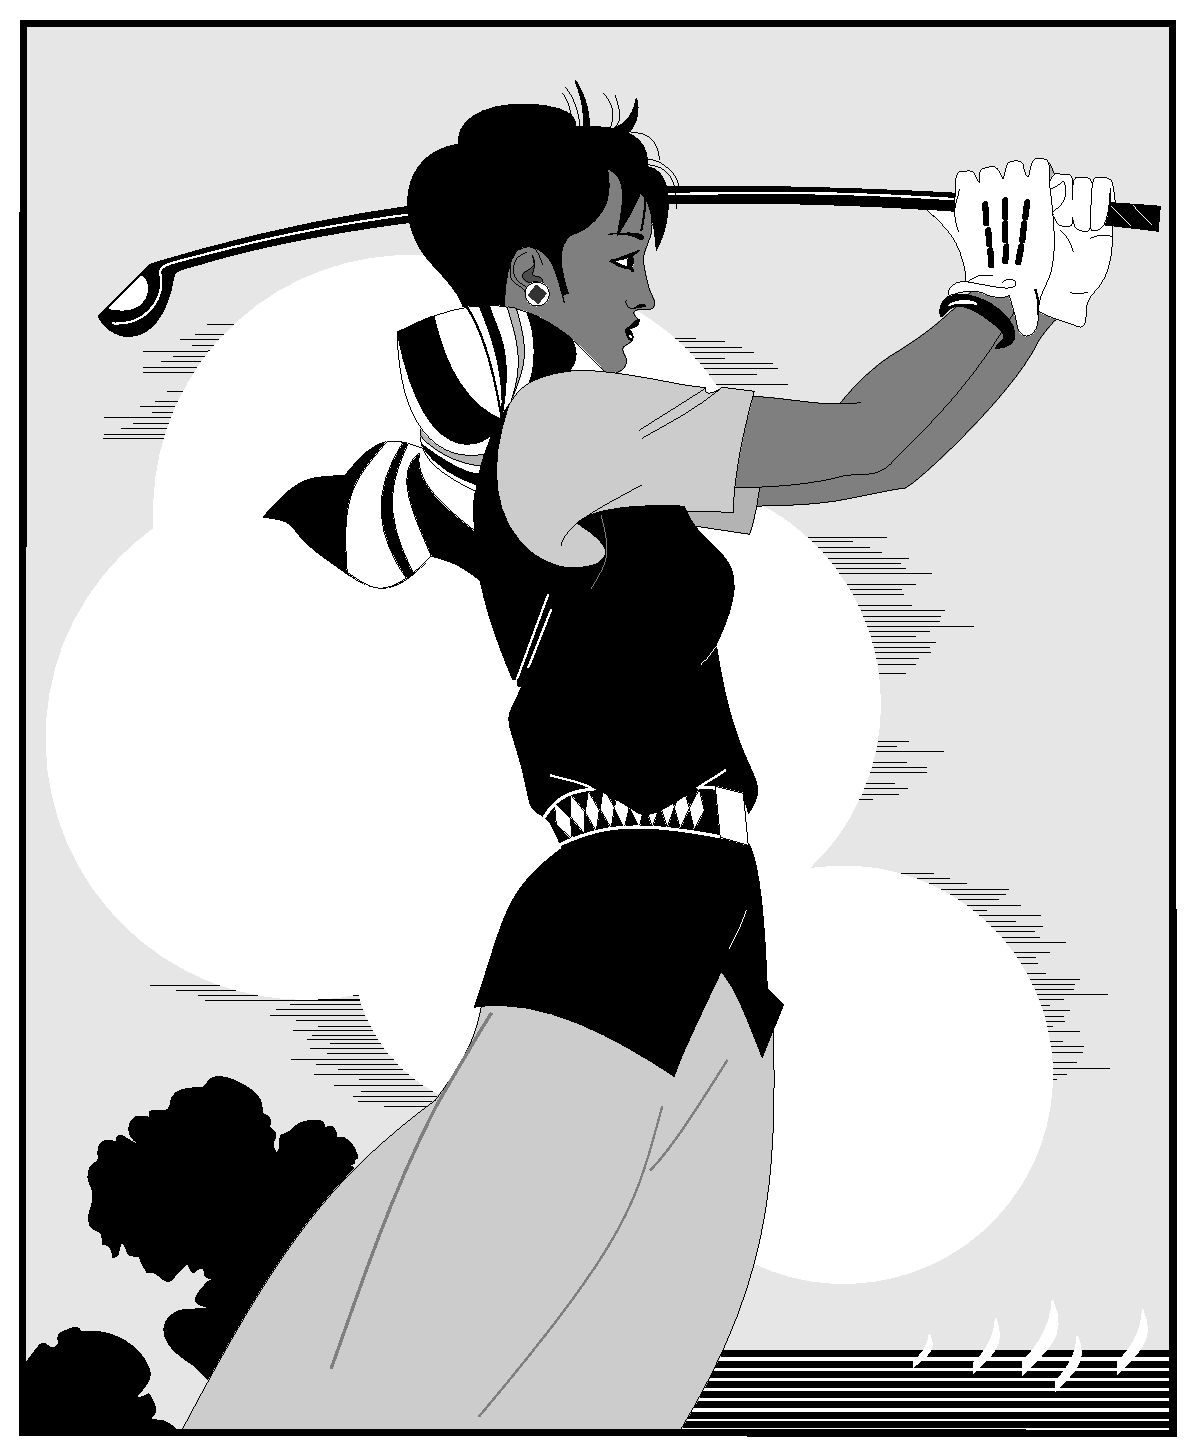
\includegraphics[width = 0.4\textwidth]{golfer}
% \bicaption[golfer1]{}{注意图中文字尽量用五号字
% }{Fig.$\!$}{The person playing golf}
% \end{figure}
% \end{latex}
% 单张单图题的格式如下,
% \begin{latex}
% \begin{figure}[h]
% \centering
% 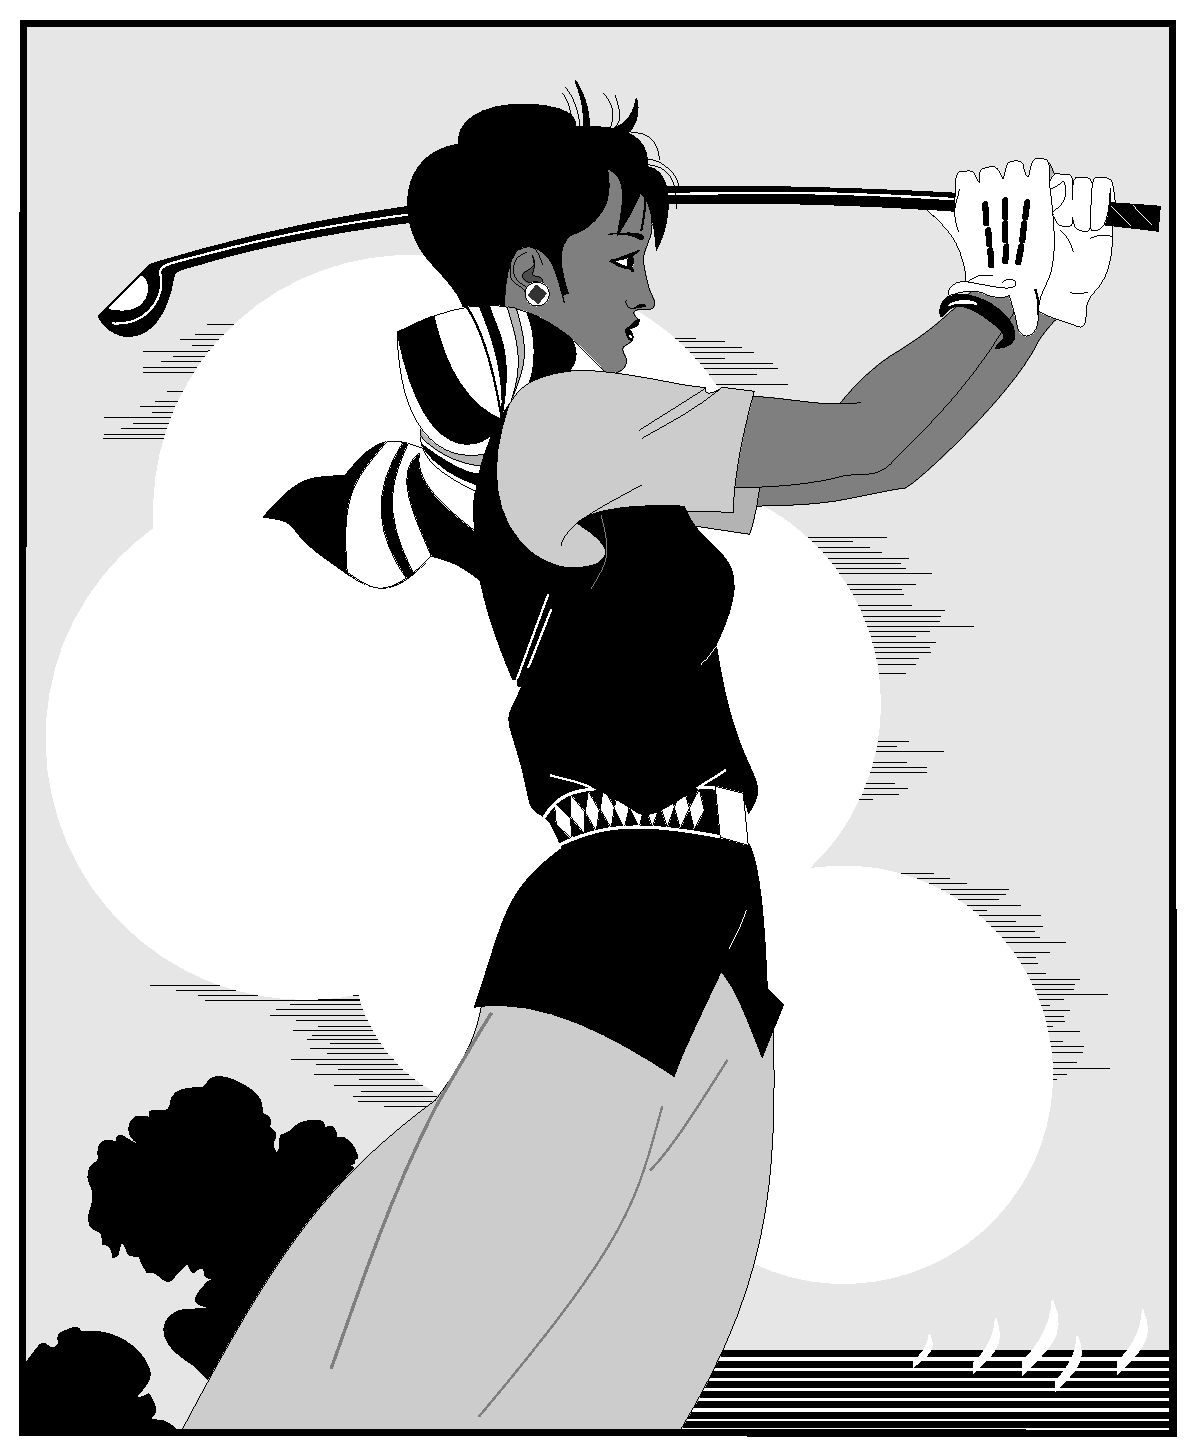
\includegraphics[width = 0.4\textwidth]{golfer}
% \caption{注意图中文字字号尽量用五号字}
% \end{figure}
% \end{latex}
% 并排图例。
% \begin{latex}
% \begin{figure}[htbp]
% \centering
% \begin{minipage}{0.4\textwidth}
% \centering
% 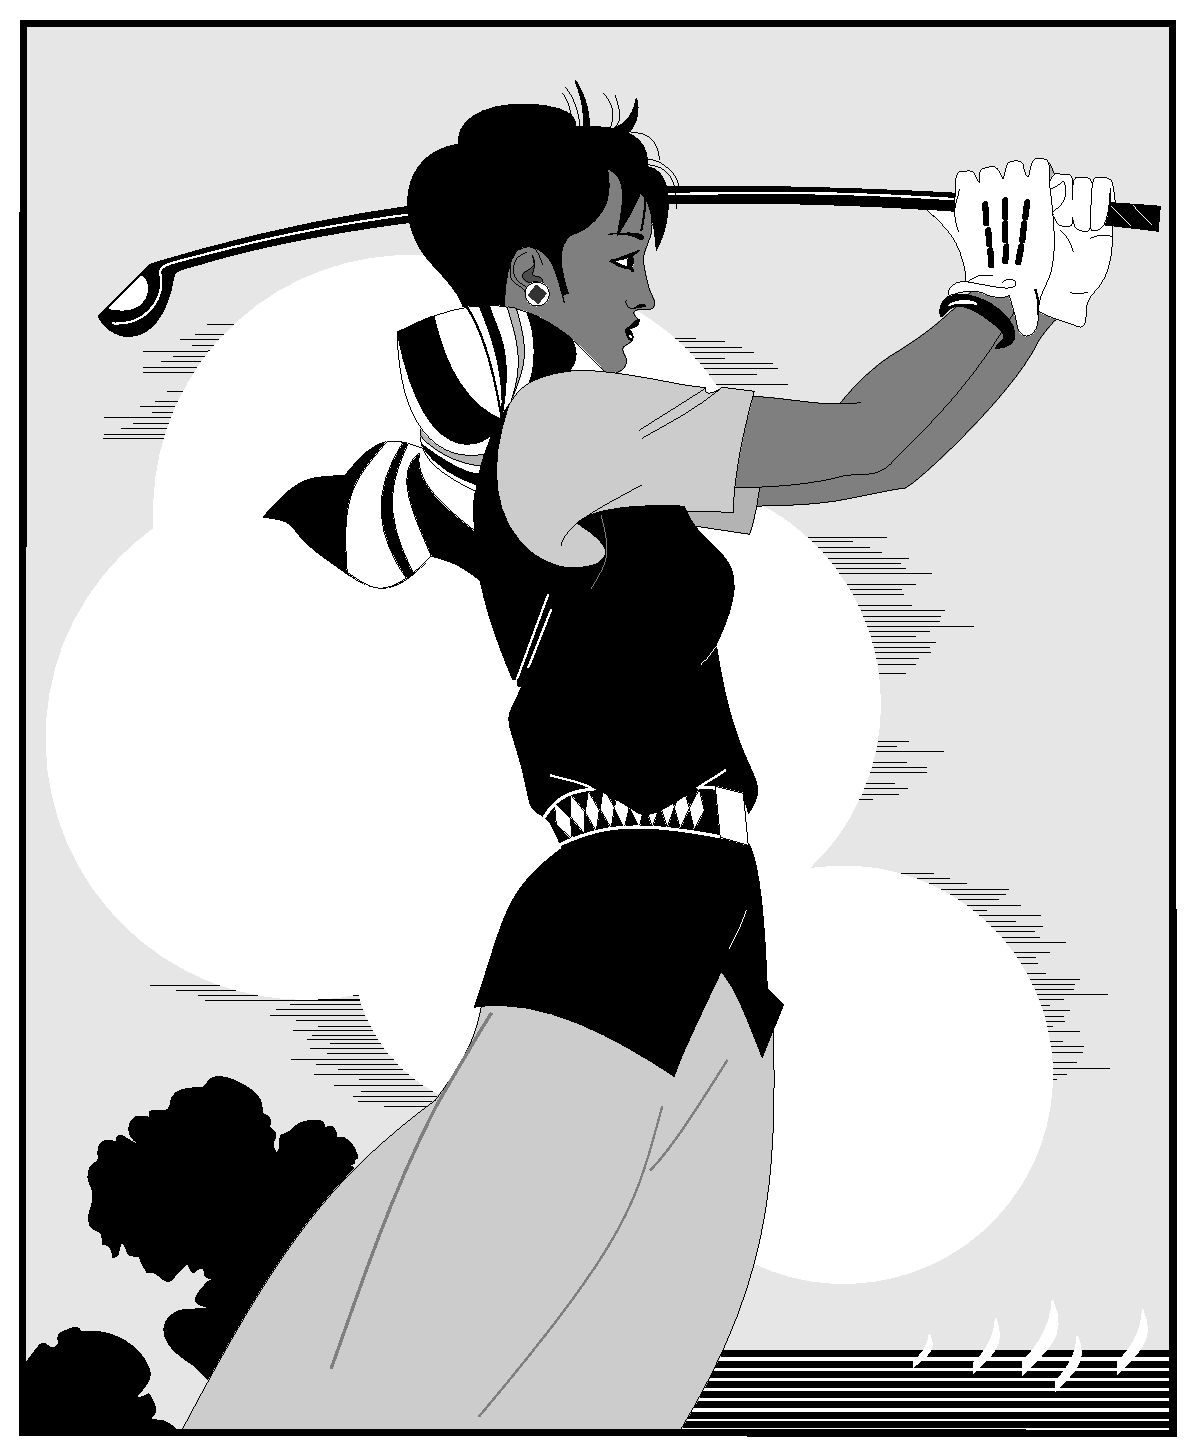
\includegraphics[width=\textwidth]{golfer}
% \bicaption[golfer2]{}{打高尔夫球的人}{Fig.$\!$}{The person playing golf}
% \end{minipage}
% \begin{minipage}{0.4\textwidth}
% \centering
% 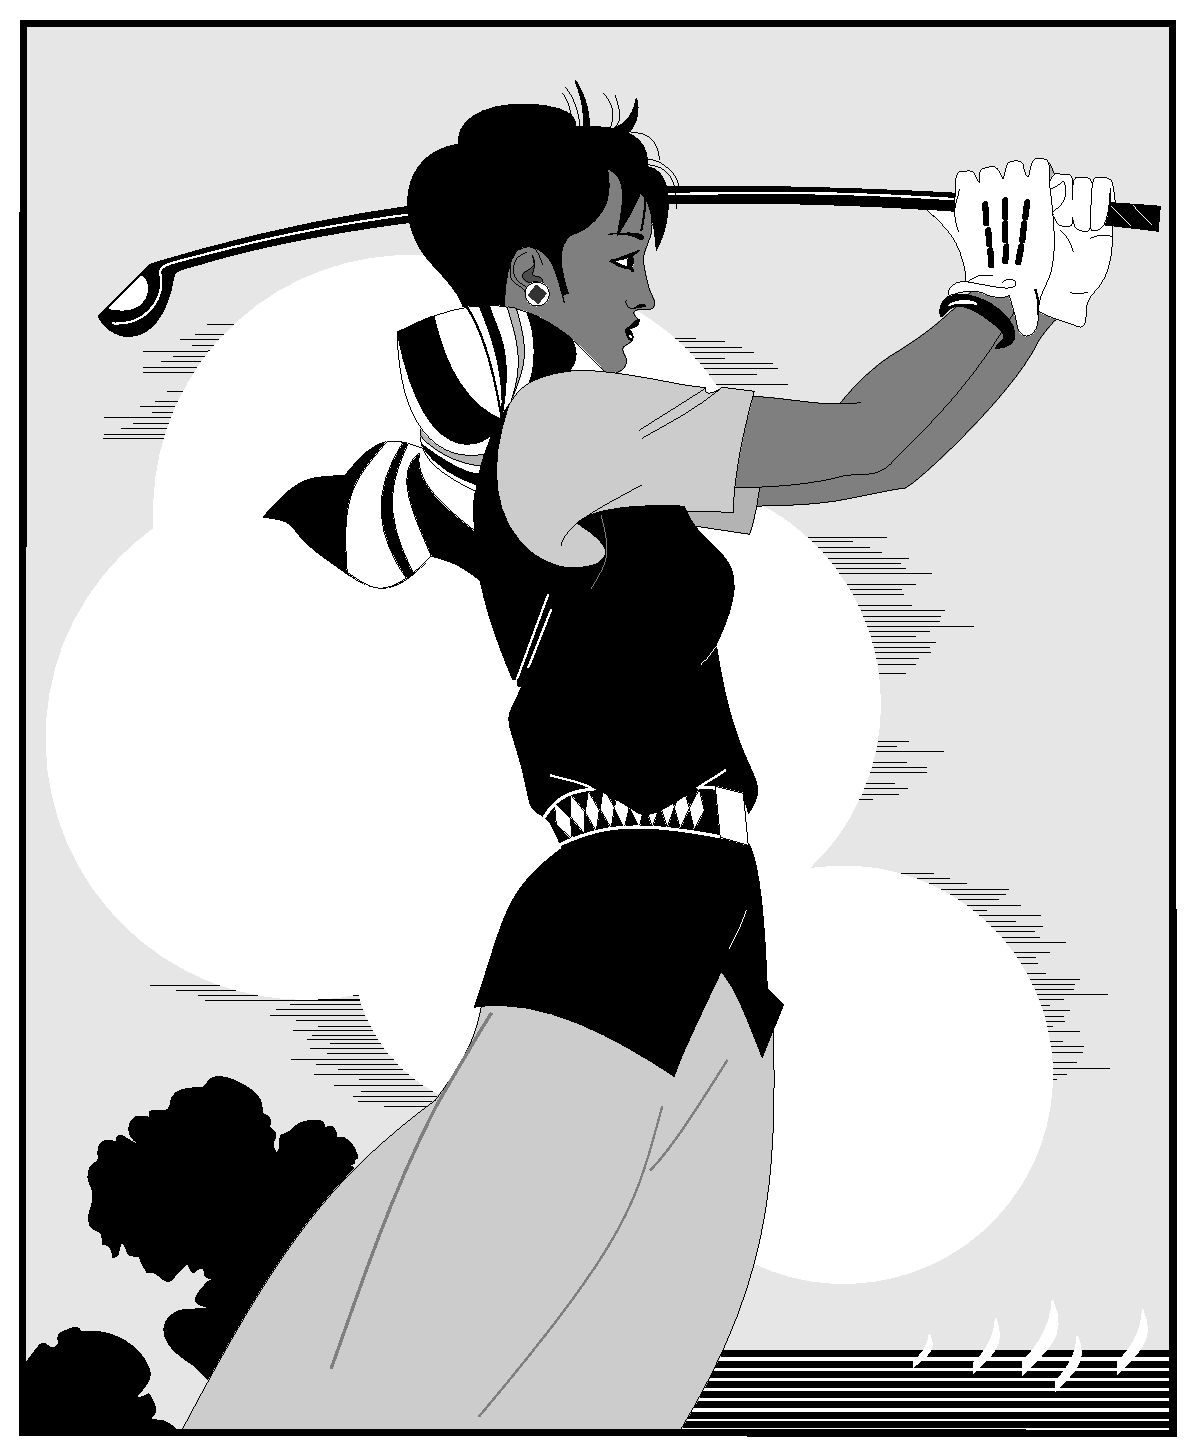
\includegraphics[width=\textwidth]{golfer}
% \bicaption[golfer3]{}{打高尔夫球的人}{Fig.$\!$}{The person playing golf}
% \end{minipage}
% \end{figure}
% \end{latex}
% 子图图例。
% \begin{latex}
% \begin{figure}[htbp]
% \centering
% \subfigure{\label{golfer41}}\addtocounter{subfigure}{-2}
% \subfigure[The person playing golf]{\subfigure[打高尔夫球的人~1]{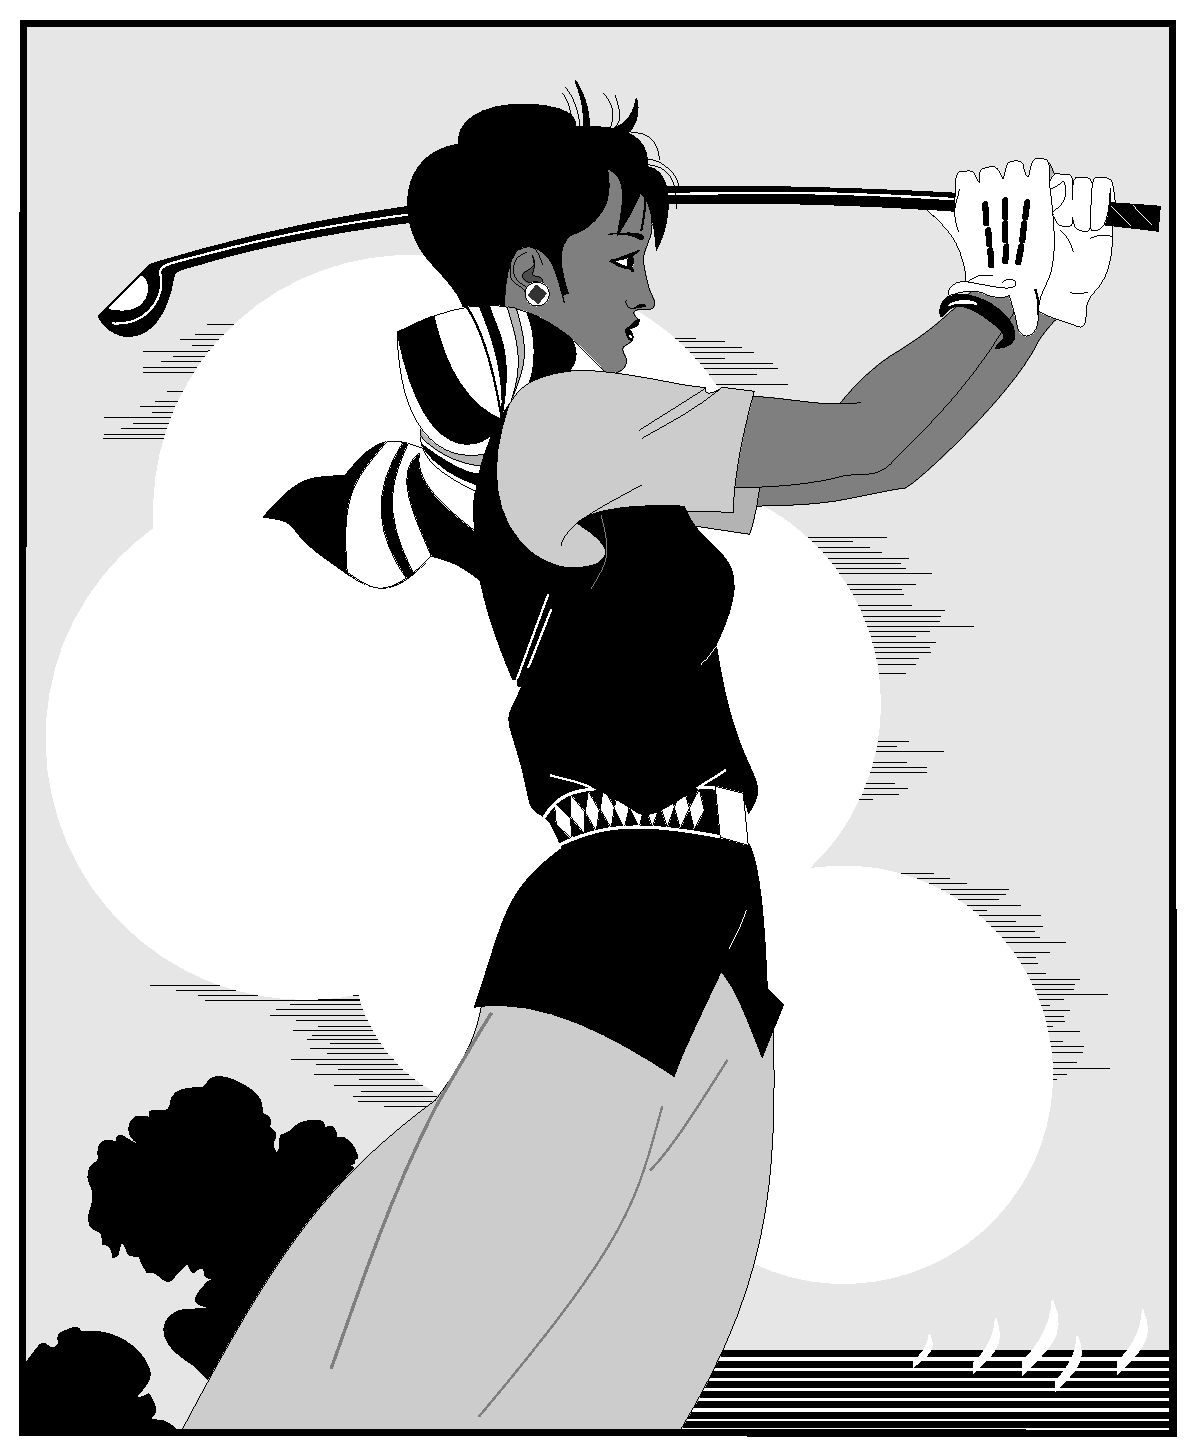
\includegraphics[width=0.4\textwidth]{golfer}}}
% \subfigure{\label{golfer42}}\addtocounter{subfigure}{-2}
% \subfigure[The person playing golf]{\subfigure[打高尔夫球的人~2]{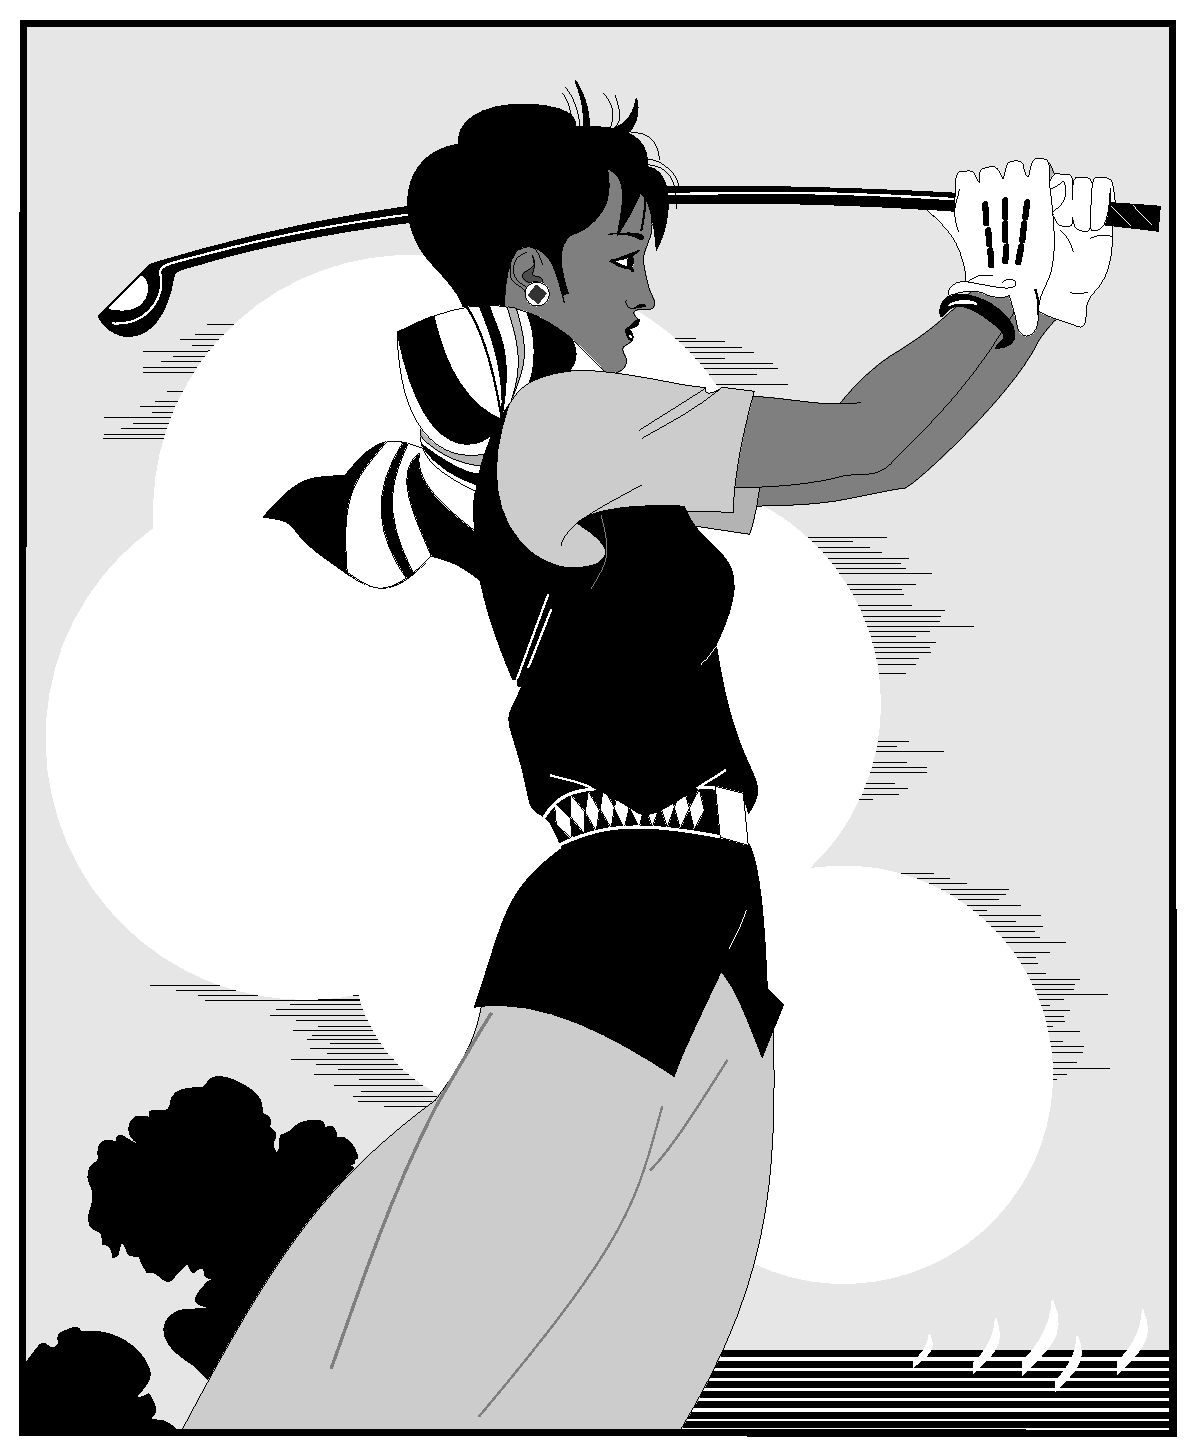
\includegraphics[width=0.4\textwidth]{golfer}}}
% \bicaption[golfer4]{}{打高尔夫球的人}{Fig.$\!$}{The person playing golf}
% \end{figure}
% \end{latex}
% 表格示例,表格中的字体是可以自行调整的。
% \begin{latex}
% \begin{table}[htbp]
% \bicaption[table1]{}{符合研究生院绘图规范的表格}{Table$\!$}{Table in agreement of the standard from graduate school}
% \vspace{0.5em}\centering\wuhao
% \begin{tabular}{ccccc}
% \toprule[1.5pt]
% $D$(in) & $P_u$(lbs) & $u_u$(in) & $\beta$ & $G_f$(psi.in)\\
% \midrule[1pt]
%  5 & 269.8 & 0.000674 & 1.79 & 0.04089\\
% 10 & 421.0 & 0.001035 & 3.59 & 0.04089\\
% 20 & 640.2 & 0.001565 & 7.18 & 0.04089\\
% \bottomrule[1.5pt]
% \end{tabular}
% \end{table}
% \end{latex}
% 因为长表格不是浮动体,不会自动调整位置、也不会自动调整字体大小,一切都要手动设
% 置。特别繁琐。
% \begin{latex}
% \ltfontsize{\dawu[1.667]} %设置表格内字体行间距
% \dawu[1.667]\begin{longtable}{ccc} % 注意此处设置的是表格线距离
% \longbionenumcaption{}{{\wuhao 中国省级行政单位一览 %此处要添加字体设置
% }\label{table2}}{Table$\!$}{}{{\wuhao Overview of the provincial administrative
% unit of China}}{-0.5em}{3.15bp}\\ %注意后两个参数分别是中英标题间距、标题和表格的间距。
% %\caption{\wuhao 中国省级行政单位一览}\\[1em] %注意此处是标题和表格间距,这行
% %是单语标题
% \toprule[1.5pt] 名称 & 简称 & 省会或首府  \\ \midrule[1pt]
% \endfirsthead
% \multicolumn{3}{r}{表~\thetable(续表)}\vspace{0.5em}\\
% \toprule[1.5pt] 名称 & 简称 & 省会或首府  \\ \midrule[1pt]
% \endhead
% \bottomrule[1.5pt]
% \endfoot
% 北京市 & 京 & 北京\\
% 天津市 & 津 & 天津\\
% 河北省 & 冀 & 石家庄市\\
% 山西省 & 晋 & 太原市\\
% 内蒙古自治区 & 蒙 & 呼和浩特市\\
% 辽宁省 & 辽 & 沈阳市\\
% 吉林省 & 吉 & 长春市\\
% 黑龙江省 & 黑 & 哈尔滨市\\
% 上海市 & 沪/申 & 上海\\
% 江苏省 & 苏 & 南京市\\
% 浙江省 & 浙 & 杭州市\\
% 安徽省 & 皖 & 合肥市\\
% 福建省 & 闽 & 福州市\\
% 江西省 & 赣 & 南昌市\\
% 山东省 & 鲁 & 济南市\\
% 河南省 & 豫 & 郑州市\\
% 湖北省 & 鄂 & 武汉市\\
% 湖南省 & 湘 & 长沙市\\
% 广东省 & 粤 & 广州市\\
% 广西壮族自治区 & 桂 & 南宁市\\
% 海南省 & 琼 & 海口市\\
% 重庆市 & 渝 & 重庆\\
% 四川省 & 川/蜀 & 成都市\\
% 贵州省 & 黔/贵 & 贵阳市\\
% 云南省 & 云/滇 & 昆明市\\
% 西藏自治区 & 藏 & 拉萨市\\
% 陕西省 & 陕/秦 & 西安市\\
% 甘肃省 & 甘/陇 & 兰州市\\
% 青海省 & 青 & 西宁市\\
% 宁夏回族自治区 & 宁 & 银川市\\
% 新疆维吾尔自治区 & 新 & 乌鲁木齐市\\
% 香港特别行政区 & 港 & 香港\\
% 澳门特别行政区 & 澳 & 澳门\\
% 台湾省 & 台 & 台北市\\
% \end{longtable}\normalsize %注意这里要恢复正常字体
% \end{latex}
% \subsubsection{公式}
% 公式不做介绍,与正常用法一致。
% \subsubsection{数学环境}
% \label{sec:math}
% \hithesis\ 定义了常用的数学环境:
%
% \begin{center}
% \begin{tabular}{*{7}{l}}\toprule
%   axiom & theorem & definition & proposition & lemma & conjecture &\\
%   公理 & 定理 & 定义 & 命题 & 引理 & 猜想 &\\\midrule
%   proof & corollary & example & exercise & assumption & remark & problem \\
%   证明 & 推论 & 例子& 练习 & 假设 & 注释 & 问题\\\bottomrule
% \end{tabular}
% \end{center}
%
% 比如:
% \begin{latex}
% \begin{definition}
%   道千乘之国,敬事而信,节用而爱人,使民以时。
% \end{definition}
% \end{latex}
% 产生(自动编号):
% \medskip
%
% \noindent\framebox[\linewidth][l]{{\heiti 定义~1.1~~~} % {道千乘之国,敬事而信,节用而爱人,使民以时。}}
%
% \smallskip
% 列举出来的数学环境毕竟是有限的,如果想用\emph{胡说}这样的数学环境,那么可以定义:
% \begin{latex}
% \newtheorem{nonsense}{胡说}[chapter]
% \end{latex}
%
% 然后这样使用:
% \begin{latex}
% \begin{nonsense}
%   契丹武士要来中原夺武林秘笈。—— 慕容博
% \end{nonsense}
% \end{latex}
% 产生(自动编号):
%
% \medskip
% \noindent\framebox[\linewidth][l]{{\heiti 胡说~1.1~~~} % {契丹武士要来中原夺武林秘笈。—— 慕容博}}
% \subsubsection{算法}
% 我工算法不在规范中要求且一千个评审老师有一千个算法格式喜好。详见
% \href{https://github.com/PlutoThesis/PlutoThesis#%E6%B2%A1%E6%9C%89%E6%98%8E%E7%A1%AE%E8%A6%81%E6%B1%82%E7%9A%84%E6%A0%BC%E5%BC%8F}{PlutoThesis}
% 中的各个实验室算法喜好举例。在此多说无益。
% \subsubsection{引用参考文献}
% \DescribeMacro{\inlinecite}
% 学校要求的参考文献引用有两种模式:(1)上标模式。比如``同样的工作有很
% 多$^{[1,2]}$\ldots''。(2)正文模式。比如``文[3] 中详细说明了\ldots''。其中上标
% 模式使用远比正文模式频繁,所以为了符合使用习惯,上标模式仍然用常规
% 的 \cs{cite}\marg{key},而 \cs{inlinecite}\marg{key} 则用来生成正文模式。
%
% 关于参考文献模板推荐使用 \BibTeX,关于中文参考文献需要额外增加一个 Entry:
% \texttt{lang},将其设置为 \texttt{zh} 用来指示此参考文献为中文,以
% 便 \file{hithesis.bst} 处理。如:
% \begin{latex}
% @INPROCEEDINGS{cnproceed,
%   author    = {王重阳 and 黄药师 and 欧阳峰 and 洪七公 and 段皇帝},
%   title     = {武林高手从入门到精通},
%   booktitle = {第~$N$~次华山论剑},
%   year      = 2006,
%   address   = {西安, 中国},
%   month     = sep,
%   lang      = "zh",
% }
%
% @ARTICLE{cnarticle,
%   AUTHOR  = "贾宝玉 and 林黛玉 and 薛宝钗 and 贾探春",
%   TITLE   = "论刘姥姥食量大如牛之现实意义",
%   JOURNAL = "红楼梦杂谈",
%   PAGES   = "260--266",
%   VOLUME  = "224",
%   YEAR    = "1800",
%   LANG    = "zh",
% }
% \end{latex}
%
% 注意如果不需要引用参考文献,请删除 \file{main.tex} 中 \cs{bibliography} 开头的两行,
% 以避免可能的编译错误。
%
% \subsubsection{列表环境}
% \DescribeEnv{itemize}
% \DescribeEnv{enumerate}
% \DescribeEnv{description}
% 为了适合中文习惯,模板将这三个常用的列表环境用 \pkg{enumitem} 进行了纵向间距压
% 缩。一方面清除了多余空间,另一方面用户可以自己指定列表环境的样式(如标签符号,
% 缩进等)。细节请参看 \pkg{enumitem} 文档,此处不再赘述。
% \subsection{后文}
%
% \subsubsection{结论}
% \DescribeEnv{conclusion}
% 结论之后为后文内容。
% \begin{latex}
% \begin{conclusions}
%
% 学位论文的结论作为论文正文的最后一章单独排写,但不加章标题序号。
%
% 结论应是作者在学位论文研究过程中所取得的创新性成果的概要总结,不能与摘要混为一
% 谈。博士学位论文结论应包括论文的主要结果、创新点、展望三部分,在结论中应概括论
% 文的核心观点,明确、客观地指出本研究内容的创新性成果(含新见解、新观点、方法创
% 新、技术创新、理论创新),并指出今后进一步在本研究方向进行研究工作的展望与设想
% 。对所取得的创新性成果应注意从定性和定量两方面给出科学、准确的评价,分(1)、
% (2)、(3)…条列出,宜用“提出了”、“建立了”等词叙述。
%
% \end{conclusions}
% \end{latex}
%
% \subsubsection{参考文献}
% 在后文中的参考文献是自动生成的,不需要用户干预,具体命令在\file{main.tex}中有
% 示例。
%
% \subsubsection{附录}
% \DescribeEnv{appendix}
% 所有的附录都插到这里来。因为附录会更改默认的 chapter 属性,而后面的{\heiti 个人简
%   历}又需要恢复,所以实现为环境可以保证全局的属性不受影响。
% \begin{latex}
% \begin{appendix}
% % -*-coding: utf-8 -*-
%%%%%%%%%%%%%%%%%%%%%%%%%%%%%%%%%%%%%%%%%%%%%%%%%%%%%%%%%
\chapter{带章节的附录}[Full Appendix]%
完整的附录内容,包含章节,公式,图表等

%%%%%%%%%%%%%%%%%%%%%%%%%%%%%%%%%%%%%%%%%%%%%%%%%%%%%%%%%
\section{附录节的内容}[Section in Appendix]
这是附录的节的内容

附录中图的示例:
\begin{figure}[htbp]
\centering
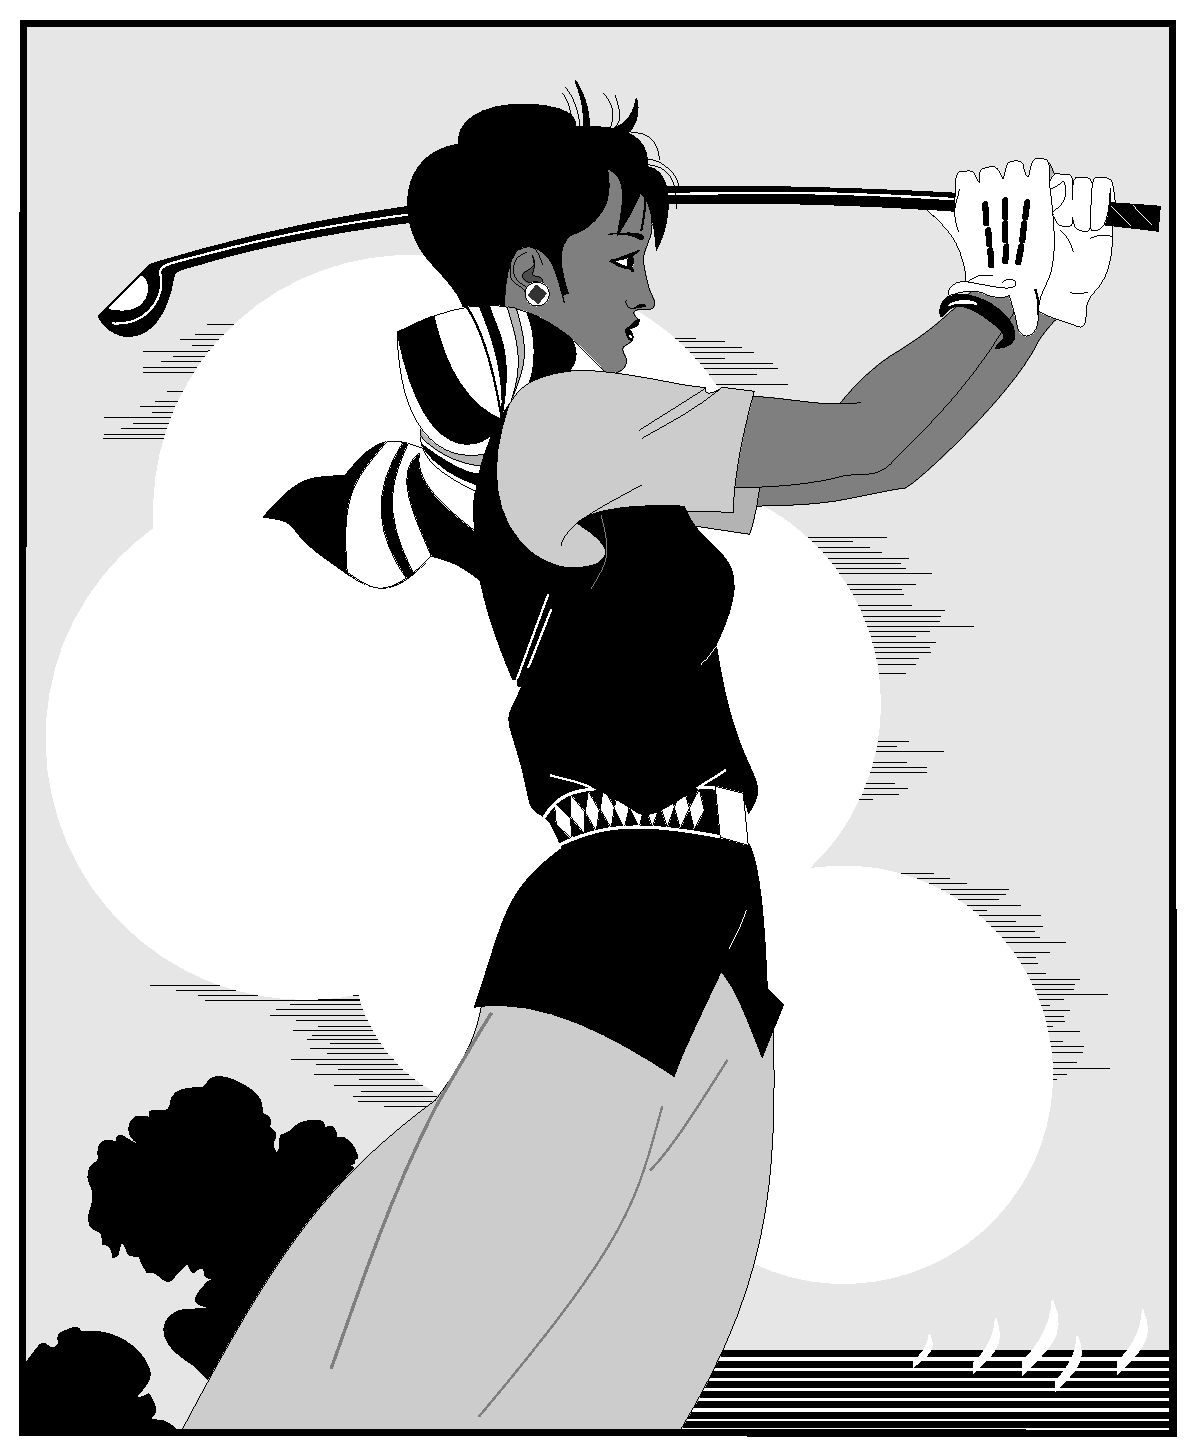
\includegraphics[width = 0.4\textwidth]{golfer}
%\bicaption[golfer5]{}{\xiaosi[0]打高尔夫球的人}{Fig.$\!$}{The person playing golf}\vspace{-1em}
\caption{\xiaosi[0]打高尔夫球的人}
\end{figure}

附录中公式的示例:
\begin{align}
a & = b \times c \\
E & = m c^2
\label{eq}
\end{align}

\chapter{这个星球上最好的免费Linux软件列表}[List of the Best Linux Software in our Planet]
\section{系统}

\href{http://fvwm.org/}{FVWM 自从上世纪诞生以来,此星球最强大的窗口管理器。}
推荐基于FVWM的桌面设计hifvwm:\href{https://github.com/dustincys/hifvwm}{https://github.com/dustincys/hifvwm}。

\subsection{hifvwm的优点}

\begin{enumerate}
	\item 即使打开上百个窗口也不会“蒙圈”。计算机性能越来越强大,窗口任务的管理必须要升级到打怪兽级别。
	\item 自动同步Bing搜索主页的壁纸。每次电脑开机,午夜零点自动更新,用户
		也可以手动更新,从此审美再也不疲劳。
	\item 切换窗口自动聚焦到最上面的窗口。使用键盘快捷键切换窗口时候,减少
		操作过程,自动聚焦到目标窗口。这一特性是虚拟窗口必须的人性化设
		计。
	\item 类似window右下角的功能的最小化窗口来显示桌面的功能此处类似
		win7/win10,实现在一个桌面之内操作多个任务。
	\item 任务栏结合标题栏。采用任务栏和标题栏结合,节省空间。
	\item 同类窗口切换。可以在同类窗口之内类似alt-tab的方式切换。
	\item ……
\end{enumerate}

\section{其他}

\href{https://github.com/goldendict/goldendict}{goldendict 星球最强大的桌面字典。}

\href{https://github.com/yarrick/iodine}{iodine,“HIT-WLAN + 锐捷”时代的福音。}

\href{http://www.aircrack-ng.org/}{aircrack,Wifi“安全性评估”工具。}

\href{https://www.ledger-cli.org/}{ledger,前“金融区块链”时代最好的复式记账系统。}

\href{https://orgmode.org/}{orgmode,最强大的笔记系统,从来没有之一。}

\href{https://www.jianguoyun.com/}{坚果云,国内一款支持WebDav的云盘系统,国内真正的云盘没有之一。}

\href{http://www.mutt.org/}{mutt, ``All mail clients suck. This one just sucks less.''}

\section{vim}
实现中英文每一句一行,以及实现每一句折叠断行的简单正则式,tex源码更加乖乖。
\begin{lstlisting}
vnoremap <leader>fae J:s/[.!?]\zs\s\+/\="\r".matchstr(getline('.'), '^\s*')/g<CR>
vnoremap <leader>fac J:s/[。!?]/\=submatch(0)."\n".matchstr(getline('.'), '^\s*')/g<CR>
vnoremap <leader>fle :!fmt -80 -s<CR>
\end{lstlisting}

% \end{appendix}
% \end{latex}
%
% \subsubsection{所发表文章}
% \DescribeEnv{publication}
% 虽然在\PGR\UGR\ 中都没有明确规定此处的格式,但按照旧模板PlutoThesis,此处格式
% 非常复杂。此处仍然使用旧模板中的设置方法。
% \begin{latex}
% \begin{publication}
% \noindent\textbf{(一)发表的学术论文}
% \begin{publist}
% \item	XXX,XXX. Static Oxidation Model of Al-Mg/C Dissipation Thermal Protection Materials[J]. Rare Metal Materials and Engineering, 2010, 39(Suppl. 1): 520-524.(SCI~收录,IDS号为~669JS,IF=0.16)
% \item XXX,XXX. 精密超声振动切削单晶铜的计算机仿真研究[J]. 系统仿真学报,2007,19(4):738-741,753.(EI~收录号:20071310514841)
% \item XXX,XXX. 局部多孔质气体静压轴向轴承静态特性的数值求解[J]. 摩擦学学报,2007(1):68-72.(EI~收录号:20071510544816)
% \item XXX,XXX. 硬脆光学晶体材料超精密切削理论研究综述[J]. 机械工程学报,2003,39(8):15-22.(EI~收录号:2004088028875)
% \item XXX,XXX. 基于遗传算法的超精密切削加工表面粗糙度预测模型的参数辨识以及切削参数优化[J]. 机械工程学报,2005,41(11):158-162.(EI~收录号:2006039650087)
% \item XXX,XXX. Discrete Sliding Mode Cintrok with Fuzzy Adaptive Reaching Law on 6-PEES Parallel Robot[C]. Intelligent System Design and Applications, Jinan, 2006: 649-652.(EI~收录号:20073210746529)
% \end{publist}
%
% \noindent\textbf{(二)申请及已获得的专利(无专利时此项不必列出)}
% \begin{publist}
% \item XXX,XXX. 一种温热外敷药制备方案:中国,88105607.3[P]. 1989-07-26.
% \end{publist}
%
% \noindent\textbf{(三)参与的科研项目及获奖情况}
% \begin{publist}
% \item	XXX,XXX. XX~气体静压轴承技术研究, XX~省自然科学基金项目.课题编号:XXXX.
% \item XXX,XXX. XX~静载下预应力混凝土房屋结构设计统一理论. 黑江省科学技术二等奖, 2007.
% \end{publist}
% %\vfill
% %\hangafter=1\hangindent=2em\noindent
% %\setlength{\parindent}{2em}
% \end{publication}
% \end{latex}
%
% \subsubsection{索引}
% \DescribeEnv{ceindex}
% 我工要求中英文双语索引。后文中的自动索引实际上不需要用户干预。
%\begin{latex}
% \begin{ceindex}
%   %如果想要手动加索引,注释掉以下这一样,用wordlist环境
% \printsubindex*
% \end{ceindex}
%\end{latex}
% 手工添加索引的方法不推荐,模板中将去除该功能。
% \subsubsection{授权}
% \DescribeMacro{\authorization}
% 授权页中的签名和日期是需要手写,不需要人工干预。具体示例在\file{main.tex}中。
%\begin{latex}
% \authorization %授权
% %\authorization[saomiao.pdf] %添加扫描页的命令,与上互斥
%\end{latex}
%
% \subsubsection{致谢声明}
% \DescribeEnv{acknowledgement}
% 把致谢做成一个环境更好一些,直接往里面写感谢的话就可以啦!
%
% \begin{latex}
% \begin{acknowledgement}
%   …
%   感谢\hit\LaTeX\ 论文模板\hithesis\ !
% \end{acknowledgement}
% \end{latex}
%
%
% \subsubsection{简历}
% \DescribeEnv{resume}
% 个人简历。
% 实际上,致谢和个人简历是自由发挥的地区,字体,文体,格式,内容,完全自己决定。
% \begin{latex}
% \begin{resume}
% XXXX~年~XX~月~XX~日出生于~XXXX。
%
% XXXX~年~XX~月考入~XX~大学~XX~院(系)XX~专业,XXXX~年~XX~月本科毕业并获得~XX~学学士学位。
%
% XXXX~年~XX~月------XXXX~年~XX~月在~XX~大学~XX~院(系)XX~学科学习并获得~XX~学硕士学位。
%
% XXXX~年~XX~月------XXXX~年~XX~月在~XX~大学~XX~院(系)XX~学科学习并获得~XX~学博士学位。
%
% 获奖情况:如获三好学生、优秀团干部、X~奖学金等(不含科研学术获奖)。
%
% 工作经历:
% \end{resume}
% \end{latex}
%
% \subsection{其它}
% 模板的配置文件 \file{hithesis.cfg} 中定义了很多固定词汇,一般无须修改。如果有特殊需求,
% 推荐在导言区使用 \cs{renewcommand}。
%
%
% \subsection{捐助}
% \changes{v1.0.1}{2017/08/27}{添加了捐助、矢量化本科论文模板的图片logo}
% 各位刀客和大侠如用的嗨,要解囊相助,请微信或支付宝参照图
% ~\ref{wct5}-\ref{zfb}~中提示操作(二维码被矢量化后之后去
% 除了头像等冗余无用的部分~)。
% \begin{figure}[h]
% \centering\includegraphics[width=0.5\textwidth]{wct5.eps}
% \caption{如果用的嗨,微信扫码捐助5元~~}
% \label{wct5}
% \end{figure}
% \begin{figure}[h]
% \centering\includegraphics[width=0.5\textwidth]{wct10.eps}
% \caption{如果用的非常嗨,微信扫码捐助10元~~}
% \label{wct10}
% \end{figure}
% \begin{figure}[h]
% \centering\includegraphics[width=0.5\textwidth]{wct1.eps}
% \caption{那个,看在熬夜写代码的份上,微信扫码捐助1元吧~~}
% \label{wct1}
% \end{figure}
% \begin{figure}[h]
% \centering\includegraphics[width=0.5\textwidth]{zfb.eps}
% \caption{支付宝不限额度}
% \label{zfb}
% \end{figure}
%
% \StopEventually{\PrintChanges\PrintIndex}
% \clearpage
%
% \section{实现细节}
%
% \subsection{基本信息}
%    \begin{macrocode}
%<cls>\NeedsTeXFormat{LaTeX2e}[1999/12/01]
%<cls>\ProvidesClass{hithesis}
%<cfg>\ProvidesFile{hithesis.cfg}
%<cls|cfg>[2018/12/05 2.0.6 Harbin Institute of Technology Thesis Template]
%    \end{macrocode}
%
% \subsection{定义选项}
% \label{sec:defoption}
%    \begin{macrocode}
%<*cls>
\RequirePackage{ifthen}
\RequirePackage{kvoptions}
\SetupKeyvalOptions{
  family=hit,
  prefix=hit@,
  setkeys=\kvsetkeys}
\newif\ifhit@bachelor
\newif\ifhit@master
\newif\ifhit@doctor
\define@key{hit}{type}{%
  \hit@bachelorfalse
  \hit@masterfalse
  \hit@doctorfalse
  \expandafter\csname hit@#1true\endcsname}
%    \end{macrocode}
%	定义stage项,区分开题、中期,默认false,为毕业论文,empty为空-去掉页眉 _added by t
%    \begin{macrocode}
\newif\ifhit@kaiti
\newif\ifhit@zhongqi
\define@key{hit}{stage}{%
  \hit@kaitifalse
  \hit@zhongqifalse
  \expandafter\csname hit@#1true\endcsname}
%    \end{macrocode}
%    设置版芯,由于窝工版芯歧义。
% \changes{v2.0.0}{2018/6/14}{此处添加geometry选项}
%    \begin{macrocode}
\newif\ifhit@geometrynewone
\newif\ifhit@geometrynewtwo
\define@key{hit}{newgeometry}{%
  \hit@geometrynewonefalse
  \hit@geometrynewtwofalse
  \expandafter\csname hit@geometrynew#1true\endcsname}
%    \end{macrocode}
% 目录中英文是否用 Arial 字体(默认关闭)。
%    \begin{macrocode}
\DeclareBoolOption[false]{arialtoc}
%    \end{macrocode}
% 章节标题中的英文是否用 Arial 字体(默认打开)。
%    \begin{macrocode}
\DeclareBoolOption[false]{arialtitle}
%    \end{macrocode}
% \changes{v1.0.3}{2017/08/29}{默认开启raggedbottom}
% \option{raggedbottom} 选项(默认开启)。如果不开启这个选项,会出现一页中尽量上
% 下对齐,段的间距大。如果开启,尽量使段间距保持一致,页面底部出现空白。
%    \begin{macrocode}
\DeclareBoolOption[true]{raggedbottom}
%    \end{macrocode}
% 在脚注标记中使用 \pkg{pifont} 的带圈数字(默认关闭)。
%    \begin{macrocode}
\DeclareBoolOption[false]{pifootnote}
%    \end{macrocode}
% 字体间距设置(默认关闭)。
%    \begin{macrocode}
\DeclareBoolOption[false]{glue}
%    \end{macrocode}
% 文科生四级目录设置(默认关闭)。
%    \begin{macrocode}
\DeclareBoolOption[false]{tocfour}
%    \end{macrocode}
% 目录中“目录”位置是否空行(默认开启)。
%    \begin{macrocode}
\DeclareBoolOption[true]{tocblank}
%    \end{macrocode}
% 章标题是否悬挂居中(默认开启)
%    \begin{macrocode}
\DeclareBoolOption[true]{chapterhang}
%    \end{macrocode}
% 是否是全日制学生(默认是)。
%    \begin{macrocode}
\DeclareBoolOption[true]{fulltime}
%    \end{macrocode}
% 是否有子标题(默认是)。
%    \begin{macrocode}
\DeclareBoolOption[false]{subtitle}
%    \end{macrocode}
% 是否开启debug模式(默认否)。如果开启,载入显示行号等的包,只为开发调试用。
%    \begin{macrocode}
\DeclareBoolOption[false]{debug}
%    \end{macrocode}
% \changes{v2.0.0}{2018/6/14}{此处删除newgeometry选项}
% 是否使用右开页(默认否)。
%    \begin{macrocode}
\DeclareBoolOption[false]{openright}
%    \end{macrocode}
% 图题和标题最后一行是否居中对其(默认是,非规范要求)。
% \changes{v1.0.6}{2017/10/25}{此处更改了选项的名称}
%    \begin{macrocode}
\DeclareBoolOption[false]{capcenterlast}
%    \end{macrocode}
% 子图图题和标题最后一行是否居中对其(默认是,非规范要求)。
% \changes{v1.0.6}{2017/10/25}{此处添加子图最后一行图题是否居中选项}
%    \begin{macrocode}
\DeclareBoolOption[false]{subcapcenterlast}
%    \end{macrocode}
% 中文目录中Abstract是否均为大写
% \changes{v1.0.13}{2018/4/5}{此处添加中文目录中Abstract是否均为大写选项}
%    \begin{macrocode}
\DeclareBoolOption[false]{absupper}
%    \end{macrocode}
%    此处添加控制本科论文的页码横线选项
% \changes{v1.0.15}{2018/06/05}{添加控制本科论文的页码横线选项}
%    \begin{macrocode}
\DeclareBoolOption[false]{bsmainpagenumberline}
\DeclareBoolOption[false]{bsfrontpagenumberline}
\DeclareBoolOption[true]{bsheadrule}
%    \end{macrocode}
%    数学字体是否使用新罗马
% \changes{v2.0.5}{2018/12/05}{添加数学字体开关}
%    \begin{macrocode}
\DeclareBoolOption[true]{newtxmath}
%    \end{macrocode}
%    此处应广大刀客要求添加一参考文献分割开关
% \changes{v2.0.3}{2018/10/08}{添加参考文献分割开关}
%    \begin{macrocode}
\DeclareBoolOption[false]{splitbibitem}
%    \end{macrocode}
% 声明字体选项。
%    \begin{macrocode}
\DeclareBoolOption[false]{customheadfancy}
%	添加customheadfancy项,可以用来自定义页眉,默认false,暂时无用  _added by t
\DeclareBoolOption[false]{noheader}
%	添加noheader项,true时可以用来去掉页眉(开题、中期报告老师可能不让留页眉),默认false,保留页眉  _added by t
\DeclareStringOption{fontset}
%    \end{macrocode}
% 将其余选项默认传递给 \pkg{ctexbook}。
%    \begin{macrocode}
\DeclareDefaultOption{\PassOptionsToClass{\CurrentOption}{ctexbook}}
%    \end{macrocode}
% 解析用户传递过来的选项,并加载 \pkg{ctexbook}。
%    \begin{macrocode}
\ProcessKeyvalOptions*
%    \end{macrocode}
% 使用 \XeTeX\ 引擎时,\pkg{fontspec} 宏包会被 \pkg{xeCJK} 自动调用。传递
% 给 \pkg{fontspec} 宏包 \option{no-math} 选项,避免部分数学符号字体自动调整
% 为 CMR。其他引擎下没有这个问题,这一行会被无视。
%    \begin{macrocode}
\PassOptionsToPackage{no-math}{fontspec}
%    \end{macrocode}
% 载入单双面打印设置,本、硕单面,博士双面。
%    \begin{macrocode}
\ifhit@bachelor
\PassOptionsToClass{oneside}{book}
\fi
\ifhit@master
\PassOptionsToClass{oneside}{book}
\fi
\ifhit@doctor
\PassOptionsToClass{twoside}{book}
\fi
%    \end{macrocode}
% \changes{v1.0.2}{2017/08/27}{添加了思源字体说明}
% 设置字体。由于宋体没有粗体,且我工模板的标题要求使用粗宋体,于是面临CTeX的经典
% 的伪粗体bug:“首次出现伪粗体字体之后的正常字体无法复制”。但如果使用自带宋体的
% 思源字体,那么不必使用伪粗体。模板只给出了新windows字体的思源字体设置,且思源
% 字体版本为Adobe版。
%    \begin{macrocode}
\ifthenelse%
{\equal{\hit@fontset}{}}%
{%
  \PassOptionsToPackage{AutoFakeBold=2}{xeCJK}
}%
{%
  \ifthenelse%
  {\equal{\hit@fontset}{siyuan}}%
  {\relax}%
  {%
    \PassOptionsToPackage{AutoFakeBold=2}{xeCJK}
  }%
  \PassOptionsToClass{fontset=\hit@fontset}{ctexbook}
}%
%    \end{macrocode}
% 使用 \pkg{ctexbook} 类,优于调用 \pkg{ctex} 宏包。
%    \begin{macrocode}
\LoadClass[a4paper,openany,UTF8,zihao=-4,scheme=plain]{ctexbook}
%    \end{macrocode}
% 用户至少要提供一个选项,指定论文类型。
%    \begin{macrocode}
\ifhit@bachelor\relax\else
  \ifhit@master\relax\else
    \ifhit@doctor\relax\else
        \ClassError{hithesis}%
                   {Please specify thesis type in option: \MessageBreak
                    type=[bachelor | master | doctor]}{}
      \fi
  \fi
\fi
%    \end{macrocode}
%
% \subsection{装载宏包}
% \label{sec:loadpackage}
%
% 引用的宏包和相应的定义。
%    \begin{macrocode}
\RequirePackage{etoolbox}
\RequirePackage{ifxetex}
\ifxetex
\else
        \ClassError{hithesis}%
                   {Please use: \MessageBreak
                    xelatex}{}
\fi
\RequirePackage{xparse}
%    \end{macrocode}
%
% \AmSTeX\ 宏包,用来排出更加漂亮的公式。
%    \begin{macrocode}
\RequirePackage{amsmath}
%    \end{macrocode}
% \pkg{newtx} 设置 Times New Roman,Helvetica。
%    \begin{macrocode}
\RequirePackage[defaultsups]{newtxtext}
%    \end{macrocode}
% 添加数学字体开关
%    \begin{macrocode}
\ifhit@newtxmath
\RequirePackage{newtxmath}
\fi
%    \end{macrocode}
% \pkg{newtx} 的 Mono 字体虽然很好看,但在论文中不常见。学校虽未要求 Mono 字体,
% 还是选择常见的 Courier 字体。由于比较新的实现 \TeX\ Gyre Cursor 会修
% 改\cs{bfdefault},导致中文加粗出问题,所以选用标准 \pkg{courier}。
%    \begin{macrocode}
\RequirePackage{courier}
%    \end{macrocode}
% 图形支持宏包。
%    \begin{macrocode}
\RequirePackage{graphicx}
%    \end{macrocode}
% \pkg{pdfpages} 宏包便于我们插入扫描后的授权页和声明页 PDF 文档。
%    \begin{macrocode}
\RequirePackage{pdfpages}
\includepdfset{fitpaper=true}
%    \end{macrocode}
% 更好的列表环境。
%    \begin{macrocode}
\RequirePackage{enumitem}       %使用enumitem宏包,改变列表项的格式
\RequirePackage{environ}
%    \end{macrocode}
% 禁止 \LaTeX 自动调整多余的页面底部空白,并保持脚注仍然在底部。
% 脚注按页编号。
%    \begin{macrocode}
\ifhit@raggedbottom
  \RequirePackage[bottom,perpage,hang]{footmisc}
  \raggedbottom
\else
  \RequirePackage[perpage,hang]{footmisc}
\fi
%    \end{macrocode}
% 脚注格式。
%    \begin{macrocode}
\ifhit@pifootnote
  \RequirePackage{pifont}
\fi
%    \end{macrocode}
% 利用 \pkg{CJKfntef} 实现汉字的下划线和盒子内两段对齐,并可以避免
% \cs{makebox}\oarg{width}\oarg{s} 可能产生的 underful boxes。
%    \begin{macrocode}
\RequirePackage{CJKfntef}
%    \end{macrocode}
% 定理类环境宏包,其中 \pkg{amsmath} 选项用来兼容 \AmSTeX\ 的宏包
%    \begin{macrocode}
\RequirePackage[amsmath,thmmarks,hyperref]{ntheorem}
%    \end{macrocode}
% 表格控制
%    \begin{macrocode}
\RequirePackage{longtable}
%    \end{macrocode}
% 使用三线表:\cs{toprule},\cs{midrule},\cs{bottomrule}。
%    \begin{macrocode}
\RequirePackage{booktabs}
%    \end{macrocode}
% 参考文献引用宏包。
%    \begin{macrocode}
\RequirePackage[sort&compress]{natbib}
%    \end{macrocode}
% 生成有书签的 pdf 及其开关,请结合 gbk2uni 避免书签乱码。
%    \begin{macrocode}
\RequirePackage{hyperref}
\hypersetup{%
  CJKbookmarks=true,
  linktoc=all,
  bookmarksnumbered=true,
  bookmarksopen=true,
  bookmarksopenlevel=1,
  breaklinks=true,
  colorlinks=false,
  plainpages=false,
  pdfborder=0 0 0}
%    \end{macrocode}
% 设置 url 样式,与上下文一致
%    \begin{macrocode}
\urlstyle{same}
%    \end{macrocode}
%
% \subsection{页面设置}
% \label{sec:layout}
% 本来这部分应该是最容易设置的,但根据我工\PGR\ 的3.8,3.4,3.2节的版芯矛盾,此处
% 设置两种版芯。
%    \begin{macrocode}
\ifhit@debug\RequirePackage[showframe]{geometry}\else\RequirePackage{geometry}\fi
\geometry{%根据PlutoThesis 原版定义而来
  a4paper, % 210 * 297mm
  hcentering,
  ignoreall,
  nomarginpar,
}
%    \end{macrocode}
%    添加版芯设置选项
%    \changes{v2.0.0}{2018/6/14}{添加版芯设置选项}
%    \begin{macrocode}
\ifhit@geometrynewtwo%
	\geometry{
	  centering,
	  text={150true mm,236true mm},
	  left=30true mm,
	  head=5true mm,
	  headsep=2true mm,
	  footskip=0true mm,
	  foot=5.2true mm
	}
\else%
	\ifhit@geometrynewone%
		\geometry{
		  centering,
		  text={150true mm,240true mm},
		  left=30true mm,
		  head=5true mm,
		  headsep=0true mm,
		  footskip=0true mm,
		  foot=0true mm
		}
	\else%
		\geometry{%根据PlutoThesis 原版定义而来
			text={150true mm,224true mm},
			top=35.5true mm,
			left=30true mm,
			head=5true mm,
			headsep=2.5true mm,
			foot=8.5true mm
		}
	\fi%
\fi%
%    \end{macrocode}
%    载入显示行号的包。
% \changes{v1.0.9}{2018/01/07}{添加debug包}
%    \begin{macrocode}
\ifhit@debug%
\RequirePackage{layout}
\RequirePackage{layouts}
\RequirePackage{lineno}
\fi
%    \end{macrocode}
% 利用 \pkg{fancyhdr} 设置页眉页脚。
%    \begin{macrocode}
\RequirePackage{fancyhdr}
%    \end{macrocode}
% 其他包,表格、数学符号包
% \changes{v1.0.6}{2017/10/25}{此处添加子图最后一行图题是否居中选项}
%    \begin{macrocode}
\RequirePackage{tabularx}
\RequirePackage{varwidth}
%    \end{macrocode}
% 此处changepage环境用来控制索引页面的左右边距,规范中给出的示例的边距要大于正文。
% \changes{v1.0.10}{2018/02/19}{修改了索引的间距,使其更符合规范中的示例}
%    \begin{macrocode}
\RequirePackage{changepage}
\RequirePackage{multicol}
\RequirePackage{amssymb}
\RequirePackage[below]{placeins}%允许上一个section的浮动图形出现在下一个section的开始部分,还提供\FloatBarrier命令,使所有未处理的浮动图形立即被处理
\RequirePackage{flafter}       % 使得所有浮动体不能被放置在其浮动环境之前,以免浮动体在引述它的文本之前出现.
\RequirePackage{multirow}       %使用Multirow宏包,使得表格可以合并多个row格
\ifhit@subcapcenterlast
\PassOptionsToPackage{centerlast}{subfigure}
\fi
\RequirePackage{subfigure}%支持子图 %centerlast 设置最后一行是否居中
\RequirePackage[subfigure]{ccaption} %支持双语标题
%    \end{macrocode}
%    中英文索引包。
%    \begin{macrocode}
\RequirePackage[makeindex]{splitidx}
\newindex[]{china}
\newindex[]{english}
%</cls>
%    \end{macrocode}
%    我工要求的索引格式。
% \changes{v1.0.10}{2018/02/19}{修改了索引的间距,使其更符合规范中的示例}
%    \begin{macrocode}
%<*ist>
headings_flag 1
heading_prefix "\{\\vskip -\\baselineskip\\centering\\normalsize\\textbf\{"
heading_suffix "\}\\par\}\\nopagebreak\\wuhao\n"
delim_0 "\\hspace*{\\fill}"
delim_1 "\\hspace*{\\fill}"
%</ist>
%    \end{macrocode}
%    排版logo。
%    \begin{macrocode}
%<cls>\RequirePackage{xltxtra}
%    \end{macrocode}
%
% \subsection{主文档格式}
% \label{sec:mainbody}
%
% \subsubsection{Three matters}
% \begin{macro}{\cleardoublepage}
% 对于 \textsl{openright} 选项,必须保证章首页右开,且如果前章末页无内容须
% 清空其页眉页脚。
%    \begin{macrocode}
%<*cls>
\let\hit@cleardoublepage\cleardoublepage
\newcommand{\hit@clearemptydoublepage}{%
  \clearpage{\pagestyle{hit@empty}\hit@cleardoublepage}
}
\let\cleardoublepage\hit@clearemptydoublepage
%    \end{macrocode}
% \end{macro}
% \begin{macro}{\frontmatter}
% \begin{macro}{\mainmatter}
% \begin{macro}{\backmatter}
% 我们的单面和双面模式与常规的不太一样。
%    \begin{macrocode}
\renewcommand\frontmatter{%
  \ifhit@openright\cleardoublepage\else\clearpage\fi
  \@mainmatterfalse
  \pagenumbering{Roman}
  \pagestyle{hit@empty}
}

\renewcommand\mainmatter{%
  \ifhit@tocblank%
  \addtocontents{toc}{\vspace{\baselineskip}} %规范中并没有这一要求,此处不应该加
  \addtocontents{toe}{\vspace{\baselineskip}}
  \fi%
  \ifhit@openright\cleardoublepage\else\clearpage\fi
  \@mainmattertrue
  \pagenumbering{arabic}
  \pagestyle{hit@headings}
}

\renewcommand\backmatter{%
  \ifhit@openright\cleardoublepage\else\clearpage\fi
  \@mainmattertrue}
%</cls>
%    \end{macrocode}
% \end{macro}
% \end{macro}
% \end{macro}
%
% \subsubsection{字体}
% \label{sec:font}
% \begin{macro}{\normalsize}
% 根据我工规定,正文小四号 (12bp) 字,行距为固定值3--4mm。
%    \begin{macrocode}
%<*cls>
\renewcommand\normalsize{%
  \@setfontsize\normalsize{12bp}{\ifhit@glue 20.50398bp \@plus 2.83465bp \@minus 0bp\else 20.50398bp\fi}%
  \abovedisplayskip=8pt
  \abovedisplayshortskip=8pt
  \belowdisplayskip=\abovedisplayskip
  \belowdisplayshortskip=\abovedisplayshortskip}
%    \end{macrocode}
% \end{macro}
%
% WORD 中的字号对应该关系如下(1bp = 72.27/72 pt):
% \begin{center}
% \begin{tabular}{llll}
% \toprule
% 初号 & 42bp & 14.82mm & 42.1575pt \\
% 小初 & 36bp & 12.70mm & 36.135 pt \\
% 一号 & 26bp & 9.17mm & 26.0975pt \\
% 小一 & 24bp & 8.47mm & 24.09pt \\
% 二号 & 22bp & 7.76mm & 22.0825pt \\
% 小二 & 18bp & 6.35mm & 18.0675pt \\
% 三号 & 16bp & 5.64mm & 16.06pt \\
% 小三 & 15bp & 5.29mm & 15.05625pt \\
% 四号 & 14bp & 4.94mm & 14.0525pt \\
% 小四 & 12bp & 4.23mm & 12.045pt \\
% 五号 & 10.5bp & 3.70mm & 10.59375pt \\
% 小五 & 9bp & 3.18mm & 9.03375pt \\
% 六号 & 7.5bp & 2.56mm & \\
% 小六 & 6.5bp & 2.29mm & \\
% 七号 & 5.5bp & 1.94mm & \\
% 八号 & 5bp & 1.76mm & \\\bottomrule
% \end{tabular}
% \end{center}
%
% \begin{macro}{\hit@def@fontsize}
% 根据习惯定义字号。用法:\cs{hit@def@fontsize}\marg{字号名称}\marg{磅数}避免了
% 字号选择和行距的紧耦合。所有字号定义时为单倍行距,并提供选项指定行距倍数。
%    \begin{macrocode}
\def\hit@def@fontsize#1#2{%
  \expandafter\newcommand\csname #1\endcsname[1][1.3]{%
    \fontsize{#2}{##1\dimexpr #2}\selectfont}}
%    \end{macrocode}
% \end{macro}
%
% \begin{macro}{\chuhao}
% \begin{macro}{\xiaochu}
% \begin{macro}{\yihao}
% \begin{macro}{\xiaoyi}
% \begin{macro}{\erhao}
% \begin{macro}{\xiaoer}
% \begin{macro}{\sanhao}
% \begin{macro}{\xiaosan}
% \begin{macro}{\sihao}
% \begin{macro}{\banxiaosi}
% \begin{macro}{\xiaosi}
% \begin{macro}{\dawu}
% \begin{macro}{\wuhao}
% \begin{macro}{\xiaowu}
% \begin{macro}{\liuhao}
% \begin{macro}{\xiaoliu}
% \begin{macro}{\qihao}
% \begin{macro}{\bahao}
% 一组字号定义。
%    \begin{macrocode}
\hit@def@fontsize{chuhao}{42bp}
\hit@def@fontsize{xiaochu}{36bp}
\hit@def@fontsize{yihao}{26bp}
\hit@def@fontsize{xiaoyi}{24bp}
\hit@def@fontsize{erhao}{22bp}
\hit@def@fontsize{xiaoer}{18bp}
\hit@def@fontsize{sanhao}{16bp}
\hit@def@fontsize{xiaosan}{15bp}
\hit@def@fontsize{sihao}{14bp}
\hit@def@fontsize{banxiaosi}{13bp}
\hit@def@fontsize{xiaosi}{12bp}
\hit@def@fontsize{dawu}{11bp}
\hit@def@fontsize{wuhao}{10.5bp}
\hit@def@fontsize{xiaowu}{9bp}
\hit@def@fontsize{liuhao}{7.5bp}
\hit@def@fontsize{xiaoliu}{6.5bp}
\hit@def@fontsize{qihao}{5.5bp}
\hit@def@fontsize{bahao}{5bp}
%</cls>
%    \end{macrocode}
% \end{macro}
% \end{macro}
% \end{macro}
% \end{macro}
% \end{macro}
% \end{macro}
% \end{macro}
% \end{macro}
% \end{macro}
% \end{macro}
% \end{macro}
% \end{macro}
% \end{macro}
% \end{macro}
% \end{macro}
% \end{macro}
% \end{macro}
% \end{macro}
% \subsubsection{页眉页脚}
% \label{sec:headerfooter}
% \begin{macro}{\hit@empty}
% \begin{macro}{\hit@plain}
% \begin{macro}{\hit@headings}
% 定义三种页眉页脚格式:
% \begin{itemize}
% \item \texttt{hit@empty}:页眉页脚都没有
% \item \texttt{hit@plain}:只显示页脚的页码。\cs{chapter} 自动调用
% \cs{thispagestyle\{hit@plain\}}。
% \item \texttt{hit@headings}:页眉页脚同时显示
% \end{itemize}
%    \begin{macrocode}
%<*cls>
\let\hit@headrule\headrule
\fancypagestyle{hit@empty}{%
  \fancyhf{}
  \let\headrule\hit@headrule%
  \renewcommand{\headrulewidth}{0pt}
  \renewcommand{\footrulewidth}{0pt}
}
%    \end{macrocode}
%    此处根据本科生模板的多种版本,提供选项自定义页码、页眉样式。
%   \changes{v1.0.15}{2018/06/05}{添加控制本科论文的页码横线选项}
%   \changes{v1.0.15}{2018/06/05}{删除冗余的页面格式}
%    \begin{macrocode}
\fancypagestyle{hit@headings}{%
  \fancyhf{}
  \ifhit@doctor
	  \ifhit@kaiti	%页眉判断-开题 _added by t
	  \fancyhead[C]{\songti\xiaowu[0]\hit@cschoolname\hit@cdegree\hit@cthesisname\hit@stagestatus}
	  \else
	  \ifhit@zhongqi	%页眉判断-中期 _added by t
	  \fancyhead[C]{\songti\xiaowu[0]\hit@cschoolname\hit@cdegree\hit@cthesisname\hit@stagestatus}
	  \else
  \fancyhead[CO]{\songti\xiaowu[0]\leftmark}
  \fancyhead[CE]{\songti\xiaowu[0]\hit@cschoolname\hit@cdegree\hit@cthesisname}%
	  \fi
	  \fi
  \fi
  \ifhit@master
	  \ifhit@kaiti	%页眉判断-开题 _added by t
	  \fancyhead[C]{\songti\xiaowu[0]\hit@cschoolname\hit@cdegree\hit@cthesisname\hit@stagestatus}
	  \else
	  \ifhit@zhongqi	%页眉判断-中期 _added by t
	  \fancyhead[C]{\songti\xiaowu[0]\hit@cschoolname\hit@cdegree\hit@cthesisname\hit@stagestatus}
	  \else
  \fancyhead[C]{\songti\xiaowu[0]\hit@cschoolname\hit@cdegree\hit@cthesisname}
  	  \fi
  	  \fi
  \fi
  \ifhit@bachelor
	  \ifhit@kaiti	%页眉判断-开题 _added by t
	  \fancyhead[C]{\songti\xiaowu[0]\hit@cschoolname\hit@bachelor@cxuewei\hit@bachelor@cthesisname\hit@stagestatus}
	  \else
	  \ifhit@zhongqi	%页眉判断-中期 _added by t
	  \fancyhead[C]{\songti\xiaowu[0]\hit@cschoolname\hit@bachelor@cxuewei\hit@bachelor@cthesisname\hit@stagestatus}
	  \else
  \fancyhead[C]{\songti\xiaowu[0]\hit@cschoolname\hit@bachelor@cxuewei\hit@bachelor@cthesisname}%
      \fi
      \fi
  \fancyfoot[C]{\xiaowu\if@mainmatter\ifhit@bsmainpagenumberline-~\thepage~-\else\thepage\fi\else\ifhit@bsfrontpagenumberline-~\thepage~-\else\thepage\fi\fi}
	  \ifhit@noheader  %单独设置noheader项,可能会有老师要求在开题、中期报告没有页眉,此处优先级高于bsheadrule	_added by t
	  \fancyhf{}
	  \renewcommand{\headrulewidth}{0pt}
	  \else
	  \ifhit@bsheadrule
	  \renewcommand{\headrule}{
	  \vskip 1.190132pt
	  \hrule\@height2.276208pt\@width\headwidth
	  \vskip 0.75pt
	  \hrule\@height.75pt\@width\headwidth
	  }
	  \else
	  \renewcommand{\headrulewidth}{0pt}
	  \fi
	  \fi
     \else
	 \ifhit@noheader  %单独设置noheader项,可能会有老师要求在开题、中期报告没有页眉	_added by t
     \fancyhf{}
	 \renewcommand{\headrulewidth}{0pt}
	 \else
	 \renewcommand{\headrule}{
	 \vskip 1.190132pt
	 \hrule\@height2.276208pt\@width\headwidth
	 \vskip 0.75pt
	 \hrule\@height.75pt\@width\headwidth
	 }
	 \fi
	 \fi
  \fancyfoot[C]{\xiaowu-~\thepage~-}

  % 此处可能和word模板不一致
  % 页眉中小五汉字,0行距时,占用9bt,页眉高度为14pt, 所以以下数字之和要保持等于14pt-9bt=4.96634pt
  % 根据PlutoThesis模板中rule宽度定义为2.25, 0.75, 保持粗线和细线之间的间距为细线宽度。
  % 如果页眉是多行的情况,rule向下溢出
  \renewcommand{\footrulewidth}{0pt}
}
\AtBeginDocument{%此处解决页眉经典bug
  \pagestyle{hit@empty}
  \renewcommand{\chaptermark}[1]{\@mkboth{\CTEXthechapter\enspace#1}{}}}
%</cls>
%    \end{macrocode}
% \end{macro}
% \end{macro}
% \end{macro}
%
% \subsubsection{段落}
% \label{sec:paragraph}
%
% 全文首行缩进 2 字符,标点符号用全角
%    \begin{macrocode}
%<*cls>
\ctexset{%
  punct=quanjiao,
  space=auto,
  autoindent=true}
%    \end{macrocode}
% 利用 \pkg{enumitem} 命令调整默认列表环境间的距离,以符合中文习惯。
%    \begin{macrocode}
\setlist{nosep}
%</cls>
%    \end{macrocode}
% \subsubsection{脚注}
% \label{sec:footnote}
% 脚注符合中文习惯,数字带圈。
%    \begin{macrocode}
%<*cls>
\def\hit@textcircled#1{%
  \ifnum\value{#1} >9
    \ClassError{hithesis}%
      {Too many footnotes in this page.}{Keep footnote less than 10.}
  \fi
  \ifhit@pifootnote%
    \ding{\the\numexpr\value{#1}+171\relax}%
  \else%
    \textcircled{\xiaoliu\arabic{#1}}%
  \fi}
\renewcommand{\thefootnote}{\hit@textcircled{footnote}}
\renewcommand{\thempfootnote}{\hit@textcircled{mpfootnote}}
%    \end{macrocode}
% 定义脚注分割线,字号(宋体小五),以及悬挂缩进(1.5字符)。
%    \begin{macrocode}
\def\footnoterule{\vskip-3\p@\hrule\@width0.3\textwidth\@height0.4\p@\vskip2.6\p@}
\let\hit@footnotesize\footnotesize
\renewcommand\footnotesize{\hit@footnotesize\xiaowu[1.5]}
\footnotemargin1.5em\relax
%    \end{macrocode}
% \cs{@makefnmark} 默认是上标样式,而在脚注部分要求为正文大小。利用\cs{patchcmd}
% 动态调整 \cs{@makefnmark} 的定义。
%    \begin{macrocode}
\let\hit@makefnmark\@makefnmark
\def\hit@@makefnmark{\hbox{{\normalfont\@thefnmark}}}
\pretocmd{\@makefntext}{\let\@makefnmark\hit@@makefnmark}{}{}
\apptocmd{\@makefntext}{\let\@makefnmark\hit@makefnmark}{}{}
%</cls>
%    \end{macrocode}
% \subsubsection{数学相关}
% \label{sec:equation}
% 允许太长的公式断行、分页等。
%    \begin{macrocode}
%<*cls>
\allowdisplaybreaks[4]
\predisplaypenalty=0  %公式之前可以换页,公式出现在页面顶部
\postdisplaypenalty=0
\renewcommand\theequation{\ifnum \c@chapter>\z@ \thechapter-\fi\@arabic\c@equation}
%    \end{macrocode}
% \changes{v2.0.3}{2018/10/08}{设置公式前后随意断页}
% 公式距前后文的距离由 4 个参数控制,参见 \cs{normalsize} 的定义。
% 同时为了让 \pkg{amsmath} 的 \cs{tag*} 命令得到正确的格式,我们必须修改这些代
% 码。\cs{make@df@tag} 是定义 \cs{tag*} 和 \cs{tag} 内部命令的。
% \cs{make@df@tag@@} 处理 \cs{tag*},我们就改它!
% \begin{latex}
% \def\make@df@tag{\@ifstar\make@df@tag@@\make@df@tag@@@}
% \def\make@df@tag@@#1{%
%   \gdef\df@tag{\maketag@@@{#1}\def\@currentlabel{#1}}}
% \end{latex}
%    \begin{macrocode}
\def\make@df@tag{\@ifstar\hit@make@df@tag@@\make@df@tag@@@}
\def\hit@make@df@tag@@#1{\gdef\df@tag{\hit@maketag{#1}\def\@currentlabel{#1}}}
\iffalse
\ifhit@bachelor
  \def\hit@maketag#1{\maketag@@@{%
    (\ignorespaces\text{\equationname\hskip0.5em}#1\unskip\@@italiccorr)}}
  \def\tagform@#1{\maketag@@@{%
    (\ignorespaces\text{\equationname\hskip0.5em}#1\unskip\@@italiccorr)\equcaption{#1}}}
\fi
\fi
\def\hit@maketag#1{\maketag@@@{(\ignorespaces #1\unskip\@@italiccorr)}}
\def\tagform@#1{\maketag@@@{(\ignorespaces #1\unskip\@@italiccorr)\equcaption{#1}}}
%    \end{macrocode}
% 修改 \cs{tagform} 会影响 \cs{eqref}。
%    \begin{macrocode}
\renewcommand{\eqref}[1]{\textup{(\ref{#1})}}
%</cls>
%    \end{macrocode}
% 定理标题使用黑体,正文使用宋体,冒号隔开。
%    \begin{macrocode}
%<*cfg>
\theorembodyfont{\normalfont}
\theoremheaderfont{\normalfont\heiti}
\theoremsymbol{\ensuremath{\square}}
\newtheorem*{proof}{证明}
\theoremstyle{plain}
\theoremsymbol{}
%    \end{macrocode}
% 此处去除了冒号,(如果需要在加上这个冒号?),反正规范中没有。
% \changes{v2.0.2}{2018/06/28}{取出了定理冒号}
%    \begin{macrocode}
\theoremseparator{}
\newtheorem{assumption}{假设}[chapter]
\newtheorem{definition}{定义}[chapter]
\newtheorem{proposition}{命题}[chapter]
\newtheorem{lemma}{引理}[chapter]
\newtheorem{theorem}{定理}[chapter]
\newtheorem{axiom}{公理}[chapter]
\newtheorem{corollary}{推论}[chapter]
\newtheorem{exercise}{练习}[chapter]
\newtheorem{example}{例}[chapter]
\newtheorem{remark}{注释}[chapter]
\newtheorem{problem}{问题}[chapter]
\newtheorem{conjecture}{猜想}[chapter]
%</cfg>
%    \end{macrocode}
% \subsubsection{浮动对象以及表格}
% \label{sec:float}
% 设置浮动对象和文字之间的距离
% \changes{v1.0.9}{2018/01/07}{修正float垂直间距bug}
%    \begin{macrocode}
%<*cls>
\setlength{\intextsep}{\ifhit@glue 8.50398bp \@plus 2.83465bp \@minus 0bp\else 8.50398bp\fi}
\setlength{\textfloatsep}{\ifhit@glue 8.50398bp \@plus 2.83465bp \@minus 0bp\else 8.50398bp\fi}
\setlength{\floatsep}{\ifhit@glue 20.50398bp \@plus 2.83465bp \@minus 0bp\else 20.50398bp\fi}
%    \end{macrocode}
%    此处设置float在p选项时间隔,此处不设置\cs{@fptop}和\cs{@fpbot}以确保居中。
% \changes{v1.0.12}{2018/04/03}{修正float为p状态时默认不居中bug}
% \changes{v2.0.4}{2018/12/04}{删除\cs{@fpsep}设置,似乎没有什么用}
% \changes{v2.0.4}{2018/12/04}{更新\cs{intextsep}\cs{textfloatsep}\cs{floatsep}间距为正文行间距}
% 下面这组命令使浮动对象的缺省值稍微宽松一点,从而防止幅度对象占据过多的文本页面,
% 也可以防止在很大空白的浮动页上放置很小的图形。
% \changes{v1.0.8}{2017/11/5}{修改附录中图、表、公式数字编码}
%    \begin{macrocode}
\g@addto@macro\appendix{\renewcommand*{\thefigure}{\thechapter-\arabic{figure}}}
\g@addto@macro\appendix{\renewcommand*{\thetable}{\thechapter-\arabic{table}}}
\g@addto@macro\appendix{\renewcommand*{\theequation}{\thechapter-\arabic{equation}}}
\renewcommand{\textfraction}{0.15}
\renewcommand{\topfraction}{0.85}
\renewcommand{\bottomfraction}{0.65}
\renewcommand{\floatpagefraction}{0.60}
%    \end{macrocode}
% 由于我工的双标题,导致标题之下多出一空白字符的距离,去除。
% \changes{v2.0.4}{2018/12/04}{更新图段后空白距离}
% \changes{v2.0.4}{2018/12/04}{删除表段后空白距离}
% \changes{v2.0.5}{2018/12/05}{删除图段后空白距离}
%    \begin{macro}{\@makecaption}
%    根据我工规范,本科和硕博的图题序号之后的空格不一样。
%    \begin{hitrgu}[\PGR][2.13.1]
% 每个图均应有图题(由图序和图名组成),图题不宜有标点符号,图名在图序之后空1个
% 半角字符排写。
%    \end{hitrgu}
%    \begin{hitrgu}[\UGR][2.13.1]
% 每个图均应有图题(由图序和图名组成),图题不宜有标点符号,图名在图序之后空1个
% 字符排写。
%    \end{hitrgu}
%    我工规范中没有明确规定是否标题是否居中对齐,这里给出一个居中选项自行调整。
% 注意,我工只规定:“居中书写”。此处不额外添加悬挂处理。
% \changes{v1.0.6}{2017/10/25}{此处更改了选项的名称}
% \changes{v1.0.7}{2017/11/4}{优化了最后一行居中算法,使其两边对齐、单词内部断行}
%    \begin{macrocode}
\long\def\@makecaption#1#2{%
  \vskip\abovecaptionskip
  \wuhao\sbox\@tempboxa{#1\ifhit@bachelor\hskip\ccwd\else\enskip\fi#2}%
  \ifdim \wd\@tempboxa >\hsize
	  \ifhit@capcenterlast%
		  \vskip 6.3bp%
		  {\setbox0=\vbox{#1\ifhit@bachelor\hskip\ccwd\else\enskip\fi#2}
			  \setbox1=\vbox{%
				  \unvbox0
				  \setbox2=\lastbox
				  \hbox to \textwidth{\hfill\unhcopy2 \unskip\unskip\hfill}
			  }
		  \unvbox1}
	  \else%
		  #1\ifhit@bachelor\hskip\ccwd\else\enskip\fi#2%
	  \fi%
    \par
  \else
  \global \@minipagefalse
  \hb@xt@\hsize{\hfil\box\@tempboxa\hfil}%
  \fi
\vskip\belowcaptionskip}
%    \end{macrocode}
%    \end{macro}
%    \begin{macro}{\longbionenumcaption}
% 长表格的双语标题是一个坑. 因为第一不能用浮动格式,只能用longtable包中的tabular
% ,这样表题只能使用表格中前两行来写。这样出现了一个问题是,中英表题的间距,标题
% 和表第一行间距,表格内部间距等多个变量的协调问题。这个问题只要使用tabular的形
% 式,就是无解的。唯一的方法就是把这些参数都给用户列出来。以下,第2,5参数为中英
% 双语标题内容,1,4为标题参数。6为中英标题间距,7为表题和表格间距。
%    \begin{macrocode}
\renewcommand*{\longbionenumcaption}[7]{%
\@if@contemptyarg{#1}{\caption{#2}}{\caption[#1]{#2}}%
\global\let\@cont@oldtablename\tablename
\gdef\tablename{#3}
\global\let\LT@c@ption\@cont@LT@nonumintoc
\\[#6]
\@if@contemptyarg{#4}{\caption{#5}}{\caption[#4]{#5}}%
\global\let\tablename\@cont@oldtablename
\global\let\LT@c@ption\@cont@oldLT@c@ption
\vspace{#7}}
%    \end{macrocode}
%    \end{macro}
%    \begin{macro}{\ltfontsize}
% 我们采用 \pkg{longtable} 来处理跨页的表格。同样我们需要设置其默认字体为五号,
% 行距设置为1.3倍行距。此处还需要提供一个设置长表格内部字体的命令。
%    \begin{macrocode}
\let\hit@LT@array\LT@array
\def\LT@array{\wuhao\hit@LT@array} % set default font size
\newcommand{\ltfontsize}[1]{\def\LT@array{#1\hit@LT@array}}
%    \end{macrocode}
%    \end{macro}
%    图表名称及格式。
%    \changes{v1.0.8}{2017/11/5}{删除冗余公式符号定义}
%    \begin{macrocode}
% \changes{v2.0.6.1a}{20181221}{修改调整图表编号,添加判断,在开题/中期时,使图表编号为 section-1的格式,而非chapter-1} % _added by t
% \begin{macrocode}
\ifhit@kaiti
\renewcommand{\thefigure}{\arabic{section}-\arabic{figure}}%使图编号为 7-1 的格式 
\renewcommand{\thetable}{\arabic{section}-\arabic{table}}%使表编号为 7-1 的格式
\else
\ifhit@zhongqi
\renewcommand{\thefigure}{\arabic{section}-\arabic{figure}}%使图编号为 7-1 的格式 
\renewcommand{\thetable}{\arabic{section}-\arabic{table}}%使表编号为 7-1 的格式
\else
\renewcommand{\thefigure}{\arabic{chapter}-\arabic{figure}}%使图编号为 7-1 的格式 %\protect{~}
\renewcommand{\thetable}{\arabic{chapter}-\arabic{table}}%使表编号为 7-1 的格式
\fi \fi
\renewcommand{\thesubtable}{(\alph{subtable})}
\renewcommand{\thesubfigure}{\alph{subfigure})}%使子图编号为 a)的格式
\renewcommand{\p@subfigure}{\thefigure~} %使子图引用为 7-1 a) 的格式,母图编号和子图编号之间用~加一个空格
% \end{macrocode}
%    \end{macrocode}
%    调整罗列环境、浮动格式、间距。
%    \begin{macrocode}
\setitemize{leftmargin=0em,itemsep=0em,partopsep=0em,parsep=0em,topsep=0em,itemindent=3em}
\setenumerate{leftmargin=0em,itemsep=0em,partopsep=0em,parsep=0em,topsep=0em,itemindent=3.5em}
\newcommand{\citeup}[1]{\textsuperscript{\cite{#1}}}
%    \end{macrocode}
% 此处删除hang caption的设置
% \changes{v1.0.6}{2017/10/25}{删除caption hang 的默认设置,因为不在规范要求中}
%    \begin{macrocode}
\captionnamefont{\wuhao}
\captiontitlefont{\wuhao}
\renewcommand{\subcapsize}{\wuhao}
\setlength{\abovecaptionskip}{0pt}%为了双标题之间的间距,不能设置
\setlength{\belowcaptionskip}{0pt}
% 自定义项目列表标签及格式 \begin{publist} 列表项 \end{publist}
\newcounter{pubctr} %自定义新计数器
\newenvironment{publist}{%%%%%定义新环境
\begin{list}{[\arabic{pubctr}]} %%标签格式
    {
     \usecounter{pubctr}
     \setlength{\leftmargin}{1.7em}     % 左边界 \leftmargin =\itemindent + \labelwidth + \labelsep
     \setlength{\itemindent}{0em}     % 标号缩进量
     \setlength{\labelsep}{0.5em}       % 标号和列表项之间的距离,默认0.5em
     \setlength{\rightmargin}{0em}    % 右边界
     \setlength{\topsep}{0ex}         % 列表到上下文的垂直距离
     \setlength{\parsep}{0ex}         % 段落间距
     \setlength{\itemsep}{0ex}        % 标签间距
     \setlength{\listparindent}{0pt} % 段落缩进量
    }}
{\end{list}}
%    \end{macrocode}
% 设置定理定义格式
% \changes{v2.0.1}{2018/6/28}{去除定理注释括号}
%    \begin{macrocode}
\renewtheoremstyle{plain}
{\item[\hskip\labelsep \theorem@headerfont ##1\ ##2\theorem@separator]}
{\item[\hskip\labelsep \theorem@headerfont ##1\ ##2\ ##3\theorem@separator]}
\theorembodyfont{\songti\rmfamily}
\theoremheaderfont{\heiti\rmfamily}
\theoremsymbol{$\square$}
\setlength{\theorempreskipamount}{0pt}
\setlength{\theorempostskipamount}{-2pt}
\setlength{\parindent}{2em}
\arraycolsep=1.6pt
%</cls>
%    \end{macrocode}
%
% \subsubsection{章节标题}
% \label{sec:theor}
%    \begin{macrocode}
%<*cfg>
\ctexset{%
  chapter/name={第,章},
  appendixname=附录,
  contentsname={目\hspace{\ccwd}录},
  listfigurename=插图索引,
  listtablename=表格索引,
  figurename=图,
  tablename=表,
  bibname=参考文献,
  indexname=索引,
}
\newcommand\listfigureename{Index of figure}
\newcommand\listtableename{Index of table}
\newcommand\listequationename{Index of equation}
\newcommand\listequationname{公式索引}
\newcommand\equationname{公式}
\newcommand{\cabstractcname}{摘\hspace{\ccwd}要}
\newcommand{\cabstractename}{Abstract (In Chinese)}
%    \end{macrocode}
% 此处删除冗余选项
% \changes{v1.0.13}{2018/4/5}{此处删除冗余的Abstract标题}
%    \begin{macrocode}
\newcommand{\eabstractcname}{Abstract}
\newcommand{\eabstractename}{Abstract (In English)}
\newcommand{\hit@ckeywords@title}{关键词:}
\def\hit@ckeywords@separator{;}
\def\hit@ekeywords@separator{,}
\let\CJK@todaysave=\today
\def\CJK@todaysmall@short{\the\year 年 \the\month 月}
\def\CJK@todaysmall{\the\year 年 \the\month 月 \the\day 日}
\def\CJK@todaybig@short{\zhdigits{\the\year}年\zhnumber{\the\month}月}
\def\CJK@todaybig{\zhdigits{\the\year}年\zhnumber{\the\month}月\zhnumber{\the\day}日}
\def\CJK@today{\CJK@todaysmall}
\renewcommand\today{\CJK@today}
\newcommand\CJKtoday[1][1]{%
  \ifcase#1\def\CJK@today{\CJK@todaysave}
    \or\def\CJK@today{\CJK@todaysmall}
    \or\def\CJK@today{\CJK@todaybig}
  \fi}
%    \end{macrocode}
% 按照word示范要求,此处使用阿拉伯数字
% \changes{v1.0.14}{2018/05/06}{修正自动生成日期bug}
%    \begin{macrocode}
\cdate{\ifhit@bachelor\CJK@todaysmall\else\CJK@todaysmall@short\fi}
\edate{\ifcase \month \or January\or February\or March\or April\or May%
       \or June\or July \or August\or September\or October\or November
       \or December\fi\unskip,\ \ \the\year}
%</cfg>
%    \end{macrocode}
% 按照我工要求,页面中标题之下不少于一行。
%    \begin{macrocode}
%<*cls>
\def\hit@title@font{%
  \ifhit@arialtitle\sffamily\else\heiti\fi}

\newcommand\hit@chapter@titleformat[1]{%开启悬挂缩进选项
    \ifthenelse%
      {\equal{#1}{\eabstractcname}}%
      {\bfseries #1}%
      %实现章标题的居中加悬挂缩进,注意,此处一定是\CTEX@chaptername\CTEX@chapter@aftername, 否则是英文标题长度
      {\ifhit@chapterhang\settowidth{\hangindent}{\CTEX@chaptername\CTEX@chapter@aftername}\hangafter=1\fi#1}%
      %{\begin{varwidth}[t]{\hit@chapter@indentboxwidth}#1\end{varwidth}}
}

\renewcommand\@afterheading{%
  \@nobreaktrue
  \everypar{%
    \if@nobreak
      \@nobreakfalse
      \clubpenalty 1
      \if@afterindent \else
        {\setbox\z@\lastbox}%
      \fi
    \else
      \clubpenalty 1
      \everypar{}%
    \fi}}
%    \end{macrocode}
% 设置一到四级标题、目录、书签格式。
%    \begin{macrocode}
\ctexset{%
  chapter={
    afterindent=true,
    pagestyle={hit@headings},
    beforeskip={28.34658bp},%一个空行 1.57481 × 18
    afterskip={24.74658bp},%0.8应该不计算间距 0.8 × 18 + 0.57481×18
    aftername=\enspace,
    format={\centering\hit@title@font\xiaoer[1.57481]},%\center 会影响之后全局
    nameformat=\relax,
    numberformat=\relax,
    titleformat=\hit@chapter@titleformat,
    fixskip=true, % 添加这一行去除默认间距
    %hang=true,
  },
  section={
    afterindent=true,
    beforeskip={\ifhit@glue 13.5bp \@plus 1.677267bp \@minus 1.157391bp \else 13.5bp \fi},%上下空0.5行
    afterskip={\ifhit@glue 13.5bp \@plus 1.677267bp \@minus 1.157391bp  \else 13.5bp \fi},
    format={\hit@title@font\ifhit@glue\fontsize{15bp}{21bp \@plus 1.677267bp \@minus 1.157391bp}\else\fontsize{15bp}{21bp}\fi\selectfont},
    aftername=\enspace,
    fixskip=true,
    break={},
  },
  subsection={
    afterindent=true,
    beforeskip={\ifhit@glue 11bp \@plus 1.842609bp \@minus 0.9920497bp \else 11bp \fi},
    afterskip={\ifhit@glue 11bp \@plus 2.33863bp \@minus 0.49602bp \else 11bp \fi},
    format={\hit@title@font\ifhit@glue\fontsize{14bp}{18bp \@plus 1.842609bp \@minus 0.9920497bp}\else\fontsize{14bp}{18bp}\fi\selectfont},
    aftername=\enspace,
    fixskip=true,
    break={},
  },
  subsubsection={
    afterindent=true,
    beforeskip={\ifhit@glue 8.50398bp \@plus 2.83465bp \@minus 0bp \else 9bp \fi},
    afterskip={\ifhit@glue 8.50398bp \@plus 2.83465bp \@minus 0bp \else 9bp \fi},
    format={\hit@title@font\normalsize},
    aftername=\enspace,
    fixskip=true,
    break={},
  },
  paragraph/afterindent=true,
  subparagraph/afterindent=true
}
%    \end{macrocode}
%    设置附表、附录格式。
% \changes{v1.0.13}{2018/4/5}{此处添加中文目录中Abstract是否均为大写选项}
%    \begin{macrocode}
\NewDocumentCommand{\hit@appendix@chapter}{s m o}{%
  \IfBooleanT{#1}%
  {
    \phantomsection
    \markboth{#2}{#2}
		    \ifthenelse%
      {\equal{#2}{\eabstractcname}}%
      {\addcontentsline{toc}{chapter}{\texorpdfstring{\ifhit@arialtitle\sffamily\heiti\else\heiti\fi \ifhit@absupper\MakeUppercase{#2}\else#2\fi}{#2}}}
      {\addcontentsline{toc}{chapter}{\texorpdfstring{\ifhit@arialtitle\sffamily\heiti\else\heiti\fi #2}{#2}}}
    \IfValueT{#3}{\addcontentsline{toe}{chapter}{\texorpdfstring{\bfseries #3}{#3}}}
    \hit@chapter*{#2}
  }
}
% 该附录命令适用于发表文章,简历等
\newcommand{\BiAppChapter}[2]    % 该附录命令适用于有章节的完整附录
{\phantomsection
 \chapter{#1}
%    \end{macrocode}
% 此处添加保护选项
% \changes{v1.0.13}{2018/4/5}{添加\cs{texorpdfstring}命令去除书签中带有格式时的警告}
%    \begin{macrocode}
 \addcontentsline{toe}{chapter}{\texorpdfstring{\bfseries \xiaosi Appendix \thechapter~~#2}{Appendix \thechapter~~#2}}
}
%    \end{macrocode}
%    设置章节命令。s: 星号,表示在目录中出不出现序号。m: 必须要有的选项,中文章
%    节名称也即目录中名称,页眉中名称,书签中的名称。o: 可选内容,没有就默认是正
%    文章节,如果有,则是英文目录中显示的内容。
%    \begin{macro}{\chapter}
%    \begin{macro}{\section}
%    \begin{macro}{\subsection}
%    \begin{macro}{\subsubsection}
%    \begin{macrocode}
\let\hit@chapter\chapter
\RenewDocumentCommand{\chapter}{s o m o}{%
  \ifhit@openright\cleardoublepage\else\clearpage\fi\phantomsection%
  \IfBooleanTF{#1}%
  {%	if \chapter*
    \hit@chapter*{#3}%
    \IfValueT{#4}{%
%    \end{macrocode}
% 此处添加保护选项
% \changes{v1.0.13}{2018/4/5}{添加\cs{texorpdfstring}命令去除书签中带有格式时的警告}
%    \begin{macrocode}
	    \addcontentsline{toe}{chapter}{\texorpdfstring{\bfseries #4}{#4}}
    }
  }%
  {%	if \chapter
    \IfNoValueTF{#2}%
    {\hit@chapter{#3}}%
    {\hit@chapter[#2]{#3}}%
    \IfValueT{#4}{%
%    \end{macrocode}
%    此处需删除章节的空白
% \changes{v1.0.5}{2017/09/20}{添加\cs{ignorespaces}选项,矫正英文目录多出一个空白而无法对其的bug}
% 此处添加保护选项
% \changes{v1.0.13}{2018/4/5}{添加\cs{texorpdfstring}命令去除书签中带有格式时的警告}
%    \begin{macrocode}
	    \addcontentsline{toe}{chapter}{\texorpdfstring{\bfseries\relax Chapter \thechapter\hspace{0.5em}\ignorespaces #4}{Chapter \thechapter\hspace{0.5em}\ignorespaces #4}}
    }
  }
}

\let\hit@section\section
\RenewDocumentCommand\section{s o m o}{
  \IfBooleanTF{#1}%
  {%	if \section*
    \hit@section*{#3}%
    \IfValueT{#4}{%
      \addcontentsline{toe}{section}{#4}
    }
  }%
  {%	if \section
    \IfNoValueTF{#2}%
    {\hit@section{#3}}%
    {\hit@section[#2]{#3}}%
    \IfValueT{#4}{%
%    \end{macrocode}
%    此处需删除章节的空白
% \changes{v1.0.5}{2017/09/18}{添加\cs{ignorespaces}选项,矫正英文目录多出一个空白而无法对其的bug}
%    \begin{macrocode}
    \addcontentsline{toe}{section}{\protect\numberline{\csname thesection\endcsname}\ignorespaces #4}
    }
  }
}

\let\hit@subsection\subsection
\RenewDocumentCommand\subsection{s o m o}{
  \IfBooleanTF{#1}%
  {%	if \subsection*
    \hit@subsection*{#3}%
    \IfValueT{#4}{%
      \addcontentsline{toe}{subsection}{#4}
    }
  }%
  {%	if \subsection
    \IfNoValueTF{#2}%
    {\hit@subsection{#3}}%
    {\hit@subsection[#2]{#3}}%
    \IfValueT{#4}{%
%    \end{macrocode}
%    此处需删除章节的空白
% \changes{v1.0.5}{2017/09/18}{添加\cs{ignorespaces}选项,矫正英文目录多出一个空白而无法对其的bug}
%    \begin{macrocode}
    \addcontentsline{toe}{subsection}{\protect\numberline{\csname thesubsection\endcsname}\ignorespaces #4}
    }
  }
}

\let\hit@subsubsection\subsubsection
\RenewDocumentCommand\subsubsection{s o m o}{
  \IfBooleanTF{#1}%
  {%	if \subsubsection*
    \hit@subsubsection*{#3}%
    \IfValueT{#4}{%
      \addcontentsline{toe}{subsubsection}{#4}
    }
  }%
  {%	if \subsubsection
    \IfNoValueTF{#2}%
    {\hit@subsubsection{#3}}%
    {\hit@subsubsection[#2]{#3}}%
    \IfValueT{#4}{%
%    \end{macrocode}
%    此处需删除章节的空白
% \changes{v1.0.5}{2017/09/18}{添加\cs{ignorespaces}选项,矫正英文目录多出一个空白而无法对其的bug}
%    \begin{macrocode}
    \addcontentsline{toe}{subsubsection}{\protect\numberline{\csname thesubsubsection\endcsname}\ignorespaces #4}
    }
  }
}
%    \end{macrocode}
%    \end{macro}
%    \end{macro}
%    \end{macro}
%    \end{macro}
%
% \subsubsection{定义封面}
% \label{sec:cov}
% 封面信息。
% \changes{v1.0.11}{2018/03/07}{更改的中文标题,根据反馈,在封面中标题需要自由
% 换行且不能影响到原创性声明。此处额外设置了一个变量ctitlecover。}
%    \begin{macrocode}
\def\hit@def@term#1{%
  \define@key{hit}{#1}{\csname #1\endcsname{##1}}
  \expandafter\gdef\csname #1\endcsname##1{%
    \expandafter\gdef\csname hit@#1\endcsname{##1}}
  \csname #1\endcsname{}}

\hit@def@term{statesecrets} %密级
\hit@def@term{natclassifiedindex}  %国内图书分类号
\hit@def@term{intclassifiedindex}  %国际图书分类号

\hit@def@term{ctitlecover} %中文标题封面
\hit@def@term{ctitle} %中文标题
\hit@def@term{csubtitle} %中文副标题
\hit@def@term{cxueke} %中文学科
\hit@def@term{cauthor} %中文作者
\hit@def@term{csupervisor} %中文导师
\hit@def@term{cassosupervisor} %中文副导师
\hit@def@term{ccosupervisor}%中文联合导师
\hit@def@term{caffil}%中文院系
\hit@def@term{csubject}%中文专业
\hit@def@term{cdate}

\hit@def@term{cstudentid}%
\hit@def@term{cstudenttype}%
\hit@def@term{ctitleone}%
\hit@def@term{ctitletwo}%


\hit@def@term{etitle} %英文标题
\hit@def@term{esubtitle} %英文标题
\hit@def@term{exueke} %英文学科
\hit@def@term{eauthor} %英文作者
\hit@def@term{esupervisor} %英文导师
\hit@def@term{eassosupervisor} %英文副导师
\hit@def@term{ecosupervisor} %英文联合导师
\hit@def@term{eaffil}
\hit@def@term{esubject}
\hit@def@term{edate}
\hit@def@term{estudenttype}
\newcommand{\hit@@cabstract}[1]{\long\gdef\hit@cabstract{#1}}
\newenvironment{cabstract}{\Collect@Body\hit@@cabstract}{}
\newcommand{\hit@@eabstract}[1]{\long\gdef\hit@eabstract{#1}}
\newenvironment{eabstract}{\Collect@Body\hit@@eabstract}{}
\def\hit@parse@keywords#1{
  \define@key{hit}{#1}{\csname #1\endcsname{##1}}
  \expandafter\gdef\csname hit@#1\endcsname{}
  \expandafter\gdef\csname #1\endcsname##1{
    \@for\reserved@a:=##1\do{
      \expandafter\ifx\csname hit@#1\endcsname\@empty\else
        \expandafter\g@addto@macro\csname hit@#1\endcsname{%
          \ignorespaces\csname hit@#1@separator\endcsname}
      \fi
      \expandafter\expandafter\expandafter\g@addto@macro%
        \expandafter\csname hit@#1\expandafter\endcsname\expandafter{\reserved@a}}}}
\hit@parse@keywords{ckeywords}
\hit@parse@keywords{ekeywords}
\def\hitsetup{\kvsetkeys{hit}}
%</cls>
%    \end{macrocode}
%   定义封面中用到的词汇。
%    \begin{macrocode}
%<*cfg>
\ifhit@doctor
\gdef\hit@cxueweishort{博}
\gdef\hit@exuewei{Doctor}
\gdef\hit@exueweier{Doctoral}
\gdef\hit@cxuewei{\hit@cxueweishort 士}
\gdef\hit@cdegree{\hit@cxueke\hit@cxuewei}
\gdef\hit@edegree{\hit@exuewei \ of \hit@exueke}
\def\hit@cauthortitle{\hit@cxueweishort 士研究生}
\fi
\ifhit@master
\gdef\hit@cxueweishort{硕}
\gdef\hit@exuewei{Master}
\gdef\hit@exueweier{Master's}
\gdef\hit@cxuewei{\hit@cxueweishort 士}
\gdef\hit@cdegree{\hit@cxueke\hit@cxuewei}
\gdef\hit@edegree{\hit@exuewei \ of \hit@exueke}
\def\hit@cauthortitle{\hit@cxueweishort 士研究生}
\fi
\def\hit@kaiti@stageheader{开题报告}% 新定义页眉开题字段  _added by t
\def\hit@zhongqi@stageheader{中期报告}	% 新定义页眉中期字段  _added by t
\ifhit@kaiti
\gdef\hit@stagestatus{开题报告}% 定义stagestatus字段  _added by t
\fi
\ifhit@zhongqi
\gdef\hit@stagestatus{中期报告}% 定义stagestatus字段  _added by t
\fi
\def\hit@bachelor@cxuewei{本科}
\def\hit@bachelor@cthesisname{毕业设计(论文)}
\def\hit@bachelor@caffiltitle{院(系)}
\def\hit@bachelor@cstudentidtitle{学号}
\def\hit@bachelor@cmajortitle{专业}
\def\hit@bachelor@csupervisortitle{指导教师}
\def\hit@bachelor@cthesistitle{题目}
\def\hit@bachelor@cstudenttitle{学生}
\def\hit@cthesisname{学位论文}
\def\hit@cschoolname{哈尔滨工业大学}
\def\hit@cschoolnametitle{授予学位单位}
\def\hit@cdatetitle{答辩日期}
\def\hit@caffiltitle{所在单位}
\def\hit@csubjecttitle{学科}
\def\hit@cdegreetitle{申请学位}
\def\hit@csupervisortitle{导师}
\def\hit@cassosupervisortitle{副导师}
\def\hit@ccosupervisortitle{联合导师}
\def\hit@title@csep{:}
\def\hit@eauthortitle{Candidate}
\def\hit@esupervisortitle{Supervisor}
\def\hit@eassosupervisortitle{Associate Supervisor}
\def\hit@ecosupervisortitle{Co Supervisor}
\def\hit@edegreetitle{Academic Degree Applied for}
\def\hit@esubjecttitle{Specialty}
\def\hit@eaffiltitle{Affiliation}
\def\hit@edatetitle{Date of Defence}
\def\hit@eschoolnametitle{Degree-Conferring-Institution}
\def\hit@eschoolname{Harbin Institute of Technology}
\def\hit@title@esep{:}
\def\hit@natclassifiedindextitle{国内图书分类号}
\def\hit@internatclassifiedindextitle{国际图书分类号}
\def\hit@secretlevel{密级}
\def\hit@schoolidtitle{学校代码}
\def\hit@schoolid{10213}
\def\hit@conclusion@ctitle{结\hspace{\ccwd}论}
\def\hit@conclusion@etitle{Conclusions}
\def\hit@bibname@etitle{References}
\def\hit@acknowledgement@ctitle{致\hspace{\ccwd}谢}
\def\hit@acknowledgement@etitle{Acknowledgements}
\def\hit@resume@ctitle{个人简历}
\def\hit@resume@etitle{Resume}
\def\hit@authorization@ctitle{哈尔滨工业大学学位论文原创性声明和使用权限}
\def\hit@authorization@etitle{Statement of copyright and Letter of authorization}
\newcommand{\hit@authorsig}{作者签名:}
\newcommand{\hit@teachersig}{导师签名:}
\newcommand{\hit@frontdate}{日期:}
\newcommand{\hit@denotation@ctitle}{物理量名称及符号表}
\newcommand{\hit@denotation@etitle}{List of physical quantity and symbol}
\newcommand{\hit@authorizationtitle}{学位论文使用权限}
\newcommand{\hit@authorizationtext}{%
学位论文是研究生在哈尔滨工业大学攻读学位期间完成的成果,知识产权归属哈尔滨工业大学。学位论文的使用权限如下:

(1)学校可以采用影印、缩印或其他复制手段保存研究生上交的学位论文,并向国家图书馆报送学位论文;(2)学校可以将学位论文部分或全部内容编入有关数据库进行检索和提供相应阅览服务;(3)研究生毕业后发表与此学位论文研究成果相关的学术论文和其他成果时,应征得导师同意,且第一署名单位为哈尔滨工业大学。

保密论文在保密期内遵守有关保密规定,解密后适用于此使用权限规定。

本人知悉学位论文的使用权限,并将遵守有关规定。}
\newcommand{\hit@declarename@bachelor}{哈尔滨工业大学本科毕业设计(论文)原创性声明}
\newcommand{\hit@authorizationtext@bachelor}{%
本人郑重声明:在哈尔滨工业大学攻读学士学位期间,所提交的毕业设计(论文)《\hit@ctitle》,是本人在导师指导下独立进行研究工作所取得的成果。对本文的研究工作做出重要贡献的个人和集体,均已在文中以明确方式注明,其它未注明部分不包含他人已发表或撰写过的研究成果,不存在购买、由他人代写、剽窃和伪造数据等作假行为。

本人愿为此声明承担法律责任。}
\newcommand{\hit@declarename}{学位论文原创性声明}
\newcommand{\hit@declaretext}{%
本人郑重声明:此处所提交的学位论文《\hit@ctitle》,是本人在导师指导下,在哈尔滨工业大学攻读学位期间独立进行研究工作所取得的成果,且学位论文中除已标注引用文献的部分外不包含他人完成或已发表的研究成果。对本学位论文的研究工作做出重要贡献的个人和集体,均已在文中以明确方式注明。}
\newcommand{\hit@datefill}{\hspace{2.5em}年\hspace{1.5em}月\hspace{1.5em}日}
\newcommand{\hit@publication@ctitle}{攻读\hit@cxuewei 学位期间发表的论文及其他成果}
\newcommand{\hit@publication@etitle}{Papers published in the period of PH.D. education}
\def\hit@index@etitle{Index}
\def\hit@hi{嗨!thesis}
\def\hit@cbraceleft{(}
\def\hit@cbraceright{)}
\def\hit@ebraceleft{(}
\def\hit@ebraceright{)}
%</cfg>
%    \end{macrocode}
% 中英文封面。
%    \begin{macrocode}
%<*cls>
\newlength{\hit@title@width}
\newcommand{\hit@put@title}[2][\hit@title@width]{%
  \begin{CJKfilltwosides}[b]{#1}#2\end{CJKfilltwosides}}


\def\hit@first@titlepage{%
  \ifhit@bachelor\hit@first@titlepage@bachelor\else\hit@first@titlepage@other\fi}
\def\hit@second@titlepage{%
  \ifhit@bachelor\hit@second@titlepage@bachelor\else\hit@second@titlepage@other\fi}
\def\hit@report@titlepage{% 定义新titlepage,区分开题/中期报告中,本科和研究生不同封面
	\ifhit@bachelor\hit@report@titlepage@bachelor\else\hit@report@titlepage@graduate\fi}
%%%%%%%%%%%%%%%%%%%%%%%%%%%%%%%%%%%%%%
% 封面代码改编自 https://github.com/dustincys/PlutoThesisProposal _added by t
% 开题/中期报告封面—研究生 _added by t
\newcommand{\hit@report@titlepage@graduate}{
	\thispagestyle{empty}
	\zihao{-2}\vspace*{10mm}
	\renewcommand{\CJKglue}{\hskip 2pt plus 0.08\baselineskip}
	\centerline{\kaishu\textbf{\hit@cschoolname}}
	\vspace{10mm}
	\centerline{\zihao{2}\songti\textbf{\hit@cdegree\hit@cthesisname\hit@stagestatus}}
	\zihao{-2}\vspace*{10mm}
	\renewcommand{\CJKglue}{\hskip 2pt plus 0.08\baselineskip}
	\centerline{\songti\textbf{题目:\rule[-4pt]{220pt}{0pt}\hspace{-220pt}\textbf\hit@ctitleone}}		
	\centerline{\hspace{0em}\songti\textbf{\textbf\hit@ctitletwo}}		
	\zihao{3}\vspace{4\baselineskip}
	\hspace*{36pt}{\songti
		\renewcommand{\arraystretch}{2.5}
		\begin{tabular}{l@{}l}
			\textbf{院\hfill 系}   & \rule[-4pt]{200pt}{1pt}\hspace{-326pt}\centerline{\textbf\hit@caffil}\\
			\textbf{学\hfill 科}     & \rule[-4pt]{200pt}{1pt}\hspace{-326pt}\centerline{\textbf\hit@csubject}\\
			\textbf{导\hfill 师}     & \rule[-4pt]{200pt}{1pt}\hspace{-326pt}\centerline{\textbf\hit@csupervisor}\\
			\textbf{研\hfill 究\hfill 生}      & \rule[-4pt]{200pt}{1pt}\hspace{-326pt}\centerline{\textbf\hit@cauthor}\\
			\textbf{学\hfill 号}  & \rule[-4pt]{200pt}{1pt}\hspace{-326pt}\centerline{\textbf\hit@cstudentid}\\
			\textbf{\hit@stagestatus 日期} & \rule[-4pt]{200pt}{1pt}\hspace{-326pt}\centerline{\textbf\hit@cdate}\\
		\end{tabular}\renewcommand{\arraystretch}{1}}
	\vfill
	\centerline{\songti\textbf{研究生院制}}
	\vspace{0.5\baselineskip}
	\centerline{\songti\textbf{二〇一四年九月}}
}
%%%%%%%%%%%%%%%%%%%%%%%%%%%%%%%%%%%%%%%
%% 目前和标准模板还有些许区别,“题目”两个字与题目的内容一同居中,而学校模板是题目两个字位置固定,而题目内容单独居中。 
%% 开题/中期报告封面—本科生 _added by t
\newcommand{\hit@report@titlepage@bachelor}{
	\thispagestyle{empty}
	\zihao{-2}\vspace*{10mm}
	\renewcommand{\CJKglue}{\hskip 3pt plus 0.08\baselineskip}
	\centering
\includegraphics[width=6.2cm]{hitlogo}
	\vfill
	\centerline{\xiaoyi\songti\textbf{\hit@bachelor@cthesisname\hit@stagestatus}}
	\vfill
	%\zihao{-2}\vspace*{10mm}
	\renewcommand{\CJKglue}{\hskip 2pt plus 0.08\baselineskip}
	\centerline{\songti\textbf{题目:\rule[-4pt]{220pt}{0pt}\hspace{-220pt}\textbf\hit@ctitleone}}
	\centerline{\hspace{0em}\songti\textbf{\textbf\hit@ctitletwo}}		
	\zihao{3}\vspace{4\baselineskip}
	\hspace*{70pt}{\songti
		\renewcommand{\arraystretch}{2.5}
		\begin{tabular}{l@{}l}
			\textbf{专\hfill 业}     & \rule[-4pt]{200pt}{1pt}\hspace{-326pt}\centerline{\textbf\hit@csubject}\\
			\textbf{学\hfill 生}      & \rule[-4pt]{200pt}{1pt}\hspace{-326pt}\centerline{\textbf\hit@cauthor}\\
			\textbf{学\hfill 号}  & \rule[-4pt]{200pt}{1pt}\hspace{-326pt}\centerline{\textbf\hit@cstudentid}\\
			\textbf{指\hfill 导\hfill 教\hfill 师}     & \rule[-4pt]{200pt}{1pt}\hspace{-326pt}\centerline{\textbf\hit@csupervisor}\\
			\textbf{日\hfill 期} & \rule[-4pt]{200pt}{1pt}\hspace{-326pt}\centerline{\textbf\hit@cdate}\\
		\end{tabular}\renewcommand{\arraystretch}{1}}
	\vfill
	\centerline{\heiti\textbf{哈尔滨工业大学教务处制}}
	\vspace{0.5\baselineskip}
}
%%%%%%%%%%%%%%%%%%%%%%%%%%%%%%%%%%%%%%%
%% 目前本科生开题/中期报告封面,和教务处模板还有区别,主要表现在题目等间距不同,底部“哈尔滨工业大学教务处制”无法设置隶
%% 书字体(虽然ctex-fontset-siyuan.def 定义了\lishu 命令,但使用报错,暂无精力调试)。 _added by t

\newcommand{\hit@first@titlepage@bachelor}{
\ifthenelse%
{\equal{\hit@fontset}{siyuan}}%
{\xiaosi[1]\vspace*{0.65em}}%
{\xiaosi[1]\textcolor[rgb]{1,1,1}{\songti{\hit@hi}}}%
  \vspace*{1.2cm}
  \begin{center}
    \parbox[t][3.4cm][t]{\textwidth}{
  \begin{center}\erhao[0]\heiti\hit@ctitlecover\end{center} }
    \parbox[t][9cm][t]{\textwidth}{
    \begin{center}\xiaoer[0]\songti\textbf{\hit@cauthor}\end{center}
  }
  \begin{center}
    \setlength{\hit@title@width}{4em}
    \heiti\xiaosi
      \begin{tabular}{rc}
	{\hit@put@title{\hit@bachelor@caffiltitle}\hit@title@csep} & \hit@caffil\\[14pt]
	{\hit@put@title{\hit@bachelor@cstudentidtitle}\hit@title@csep} & \hit@cstudentid
    \end{tabular}
      \begin{tabular}{rc}
	{\hit@put@title{\hit@bachelor@cmajortitle}\hit@title@csep} & \hit@csubject\\[14pt]
	{\hit@put@title{\hit@bachelor@csupervisortitle}\hit@title@csep} &  \hit@csupervisor
      \end{tabular}
    \end{center}
    \vspace{2.6cm}
    {\xiaosi[0]\songti\textbf{\hit@cdate}}
  \end{center}
}
%    \end{macrocode}
% 此处本科生使用了\hit\ 的logo且本科生论文标题使用了华文新魏字体,为了方便使用,
% 此处使用了矢量化图片作为输入。
% \changes{v1.0.11}{2018/03/07}{更改的中文标题,根据反馈,在封面中标题需要自由
% 换行且不能影响到原创性声明。此处额外设置了一个变量ctitlecover。}
%    \begin{macrocode}
\newcommand{\hit@second@titlepage@bachelor}{
  \vspace*{0.8cm}
  \centering
\includegraphics[width=6.2cm]{hitlogo}
  \vspace{1.3cm}
  \begin{center}
    \centering
\includegraphics[width=10.5cm]{bthesistitle}
    \vfill
    \parbox[t][14.2cm][b]{\textwidth}
    {\heiti\xiaosan
      \begin{center} \renewcommand{\arraystretch}{2.5} \heiti
	\setlength{\hit@title@width}{5.5em}
	\begin{tabular}{l@{\ \  }c}

	  {\xiaoer  \hit@put@title{\hit@bachelor@cthesistitle}} & \underline{\makebox[6.1cm]{\xiaoer \hit@ctitleone}}\\
								     &  \underline{\makebox[6.1cm]{\xiaoer \hit@ctitletwo}}\\
									    & \\
	  {\hit@put@title{\hit@bachelor@cmajortitle}}                  & \underline{\makebox[6.1cm]{\hit@csubject}}\\
	  {\hit@put@title{\hit@bachelor@cstudentidtitle}}                  & \underline{\makebox[6.1cm]{\hit@cstudentid}}\\
	  {\hit@put@title{\hit@bachelor@cstudenttitle}}                  & \underline{\makebox[6.1cm]{\hit@cauthor}}\\
	  {\hit@put@title{\hit@bachelor@csupervisortitle}} & \underline{\makebox[6.1cm]{\hit@csupervisor}}\\
	  {\hit@put@title{\hit@cdatetitle}} & \underline{\makebox[6.1cm]{\hit@cdate}}
	\end{tabular} \renewcommand{\arraystretch}{1}
      \end{center}
    }
  \end{center}
}
\newlength{\hit@etitlelength}%
\newcommand{\hit@first@titlepage@other}{
  % 封面一
\ifthenelse%
{\equal{\hit@fontset}{siyuan}}%
{\xiaosi[1]\vspace*{0.65em}}%
{\xiaosi[1]\textcolor[rgb]{1,1,1}{\songti{\hit@hi}}}%
 \vspace*{1.2cm}
\begin{center}
  \begin{center}\xiaoyi[1]\songti\textbf{\hit@cxuewei\hit@cthesisname}\end{center}
    \ifhit@fulltime\vspace{1.4cm}\else%
      \begin{center}\xiaoyi[1]\songti\textbf{\hit@cbraceleft\hit@cstudenttype\hit@cbraceright}\end{center}
    \fi%
    \parbox[t][7.8cm][t]{\textwidth}{%
  \begin{center}\erhao\heiti\hit@ctitlecover\end{center}
\ifhit@subtitle\begin{center}\hspace{-4em}\xiaoer\heiti\pozhehao\hit@csubtitle\end{center}\fi
  \begin{center}%
    \settowidth{\hit@etitlelength}{\erhao\hit@etitle\ifhit@subtitle\hit@title@esep\hit@esubtitle\fi}%
    \ifdim\hit@etitlelength>450mm\xiaoer\else\erhao\fi%
    \textbf{\MakeUppercase{\hit@etitle}%
\ifhit@subtitle\hit@title@esep\MakeUppercase{\hit@esubtitle}\fi}\end{center}}

    \parbox[t][7.4cm][t]{\textwidth}{
  \begin{center}\xiaoer\songti\textbf{\hit@cauthor}\end{center}}
    \parbox[t][1.4cm][t]{\textwidth}{
  \begin{center}\kaishu\xiaoer\textbf{\hit@cschoolname}\end{center}}
    {\songti\xiaoer\textbf{\hit@cdate}}
\end{center}
}

%内封
\newcommand{\hit@second@titlepage@other}{
  \begin{center}
    {\songti \xiaosi
      \begin{tabular}{@{}r@{:}l@{}}
	\hit@natclassifiedindextitle & \hit@natclassifiedindex\\
	\hit@internatclassifiedindextitle & \hit@intclassifiedindex
    \end{tabular}}\hfill
    {\songti \xiaosi
      \begin{tabular}{@{}r@{:}l@{}}
	\hit@schoolidtitle & \hit@schoolid\\
	\hit@secretlevel & \hit@statesecrets
    \end{tabular}}
  \parbox[t][3.2cm][t]{\textwidth}{\begin{center} \end{center} }
    \parbox[t][2.4cm][t]{\textwidth}{\xiaoer[1]
  \begin{center}\songti\bfseries\hit@cdegree\hit@cthesisname\end{center}
      \ifhit@fulltime\relax\else\begin{center}\songti\textbf{\hit@cbraceleft\hit@cstudenttype\hit@cbraceright}\end{center}\fi}
	\parbox[t][5cm][t]{\textwidth}{\erhao
  \begin{center}\heiti\hit@ctitlecover\end{center}
\ifhit@subtitle\begin{center}\hspace{-4em}\xiaoer\heiti\pozhehao\hit@csubtitle\end{center}\fi}
    \parbox[t][9.8cm][b]{\textwidth}
    {\sihao
      \setlength{\hit@title@width}{6em}
      \begin{center} \renewcommand{\arraystretch}{1.62} \songti
	\begin{tabular}{l@{\hit@title@csep}l}
	  {\heiti \hit@put@title{\hit@cauthortitle}}	&	\hit@cauthor\\
	  {\heiti \hit@put@title{\hit@csupervisortitle}}	&	\hit@csupervisor\\
        \ifx\hit@cassosupervisor\@empty\else%
	  {\heiti \hit@put@title{\hit@cassosupervisortitle}}&	\hit@cassosupervisor\\
        \fi
        \ifx\hit@ccosupervisor\@empty\else%
	  {\heiti \hit@put@title{\hit@ccosupervisortitle}}	&	\hit@ccosupervisor\\
        \fi
	  {\heiti \hit@put@title{\hit@cdegreetitle}}	&	\hit@cdegree\\
	  {\heiti \hit@put@title{\hit@csubjecttitle}}	&	\hit@csubject\\
	  {\heiti \hit@put@title{\hit@caffiltitle}}		&	\hit@caffil\\
	  {\heiti \hit@put@title{\hit@cdatetitle}}		&	\hit@cdate\\
	  {\heiti \hit@put@title{\hit@cschoolnametitle}}	&	\hit@cschoolname
	\end{tabular} \renewcommand{\arraystretch}{1}
    \end{center} }
  \end{center}
}
% 英文封面
\newcommand{\emultiline}[2][c]{\renewcommand{\arraystretch}{1}\begin{tabular}[#1]{@{}l@{}}#2\end{tabular} \renewcommand{\arraystretch}{1.3}}
\newcommand{\hit@engcover}{
  {
    \xiaosi[1.667]\noindent Classified Index: \hit@natclassifiedindex \\[8pt]
  U.D.C:  \hit@intclassifiedindex }
  \vspace*{1em}
  \begin{center}
  \parbox[t][1.6cm][t]{\textwidth}{\begin{center} \end{center} }
    \parbox[t][3.5cm][t]{\textwidth}{\xiaoer[1]
  \begin{center}Dissertation for the {\hit@exueweier} Degree in \hit@exueke\end{center}
      \ifhit@fulltime\relax\else\begin{center}\hit@ebraceleft\hit@estudenttype\hit@ebraceright\end{center}\fi} %与中文保持一致,删除in {\hit@exueke}
    \parbox[t][7cm][t]{\textwidth}{%
   \begin{center}%
    \settowidth{\hit@etitlelength}{\erhao\hit@etitle\ifhit@subtitle\hit@title@esep\hit@esubtitle\fi}%
    \ifdim\hit@etitlelength>450mm\xiaoer\else\erhao\fi%
    \textbf{\MakeUppercase{\hit@etitle}%
\ifhit@subtitle\hit@title@esep\MakeUppercase{\hit@esubtitle}\fi}\end{center}}
    %★★★★若信息内容不太长,不会引起信息内容分行时,使用tabular环境,否则使用下面的tabularx环境。
    {\sihao\renewcommand{\arraystretch}{1.3}
      \begin{tabular}{@{}l@{~}l@{}}
	\textbf{\hit@eauthortitle\hit@title@esep}		&	\hit@eauthor\\
	\textbf{\hit@esupervisortitle\hit@title@esep}	&	\hit@esupervisor\\
      \ifx\hit@eassosupervisor\@empty\else%
	\textbf{\hit@eassosupervisortitle\hit@title@esep}	&	\hit@eassosupervisor\\
      \fi
      \ifx\hit@ecosupervisor\@empty\else%
	\textbf{\hit@ecosupervisortitle\hit@title@esep}	&	\hit@ecosupervisor\\
      \fi
	\textbf{\hit@edegreetitle\hit@title@esep}		&	\hit@edegree\\
      \textbf{\hit@esubjecttitle\hit@title@esep}		&\hit@esubject\\
	\textbf{\hit@eaffiltitle\hit@title@esep}		&\hit@eaffil\\
	\textbf{\hit@edatetitle\hit@title@esep}		&	\hit@edate\\
	\textbf{\hit@eschoolnametitle\hit@title@esep}	&	\hit@eschoolname
    \end{tabular}\renewcommand{\arraystretch}{1}}
  \end{center}
}
%%%%%%%%%%%%%%%%%%%%%%%%%%%%%%%%%%%%%%%%%%%%%%%%%%
%% 添加开题、中期报告封面判断样式 _added by t
\ifhit@kaiti
\def\makecover{
\begin{titlepage}	% 测试自定义的开题封面样式 _added by t 
	\hit@report@titlepage
\end{titlepage}
}
\renewcommand\thesection{\arabic {section}.}
\renewcommand\thesubsection{\thesection \arabic {subsection}}	% 	此处去除chapter继承编号,开题/中期报告只有section _added by t
\setcounter{page}{0}	% 重置页数计数器,使目录页页码从1开始
\else
\ifhit@zhongqi
\def\makecover{
	\begin{titlepage}	% 测试自定义的开题封面样式 _added by t 
		\hit@report@titlepage
	\end{titlepage}
}
\renewcommand\thesection{\arabic {section}.}
\renewcommand\thesubsection{\thesection \arabic {subsection}}	% 	此处去除chapter继承编号,开题/中期报告只有section _added by t
\setcounter{page}{0}	% 重置页数计数器,使目录页页码从1开始 _added by t
\else
%% 下为原正常论文封面 _added by t
\def\makecover{
  \phantomsection
  \pdfbookmark[0]{\hit@ctitle}{ctitle}
  \xiaosi[1]%
  \begin{titlepage}
    \hit@first@titlepage
    \cleardoublepage
    \hit@second@titlepage
    \cleardoublepage
    \ifhit@bachelor
    \relax
    \else
    \phantomsection
    \pdfbookmark[0]{\hit@etitle}{etitle}
    \hit@engcover
    \cleardoublepage
    \fi
  \end{titlepage}
  \normalsize
\hit@makeabstract}
\fi
\fi
%%%%%%%%%%%%%%%%%%%%%%%%%%%%%%%%%%%%%%%%%%%%%%%%%%
%    \end{macrocode}
%    生成参考文献和关键字。
%    \begin{macrocode}
\newbox\hit@kw
\newcommand\hit@put@keywords[2]{%
  \begingroup
    \setbox\hit@kw=\hbox{#1}
    \noindent\hangindent\wd\hit@kw\hangafter1%
    \box\hit@kw#2\par
  \endgroup}

\newcommand{\hit@makeabstract}{%
  \ifhit@openright\cleardoublepage\else\clearpage\fi
  \hit@appendix@chapter*{\cabstractcname}[\cabstractename]
  \pagestyle{hit@headings}
  \pagenumbering{Roman}
  \hit@cabstract
  \vskip12bp
  \hit@put@keywords{\heiti\hit@ckeywords@title}{\hit@ckeywords}
  \ifhit@openright\cleardoublepage\else\clearpage\fi
  \hit@appendix@chapter*{\eabstractcname}[\eabstractename]
  \hit@eabstract
  \vskip12bp
  \hit@put@keywords{\textbf{Keywords:\enskip}}{\hit@ekeywords}}
%    \end{macrocode}
%    定义符号表。
%    \begin{macrocode}
\newenvironment{denotation}[1][2.5cm]{%
  \ifhit@openright\cleardoublepage\else\clearpage\fi
  \hit@appendix@chapter*{\hit@denotation@ctitle}[\hit@denotation@etitle]
\setcounter{table}{0}
\renewcommand{\thetable}{\arabic{table}}%使表编号为 1 的格式
  }{\renewcommand{\thetable}{\arabic{chapter}-\arabic{table}}%使表编号为 7-1 的格式
\setcounter{table}{0}}%
%    \end{macrocode}
% 定义索引、目录格式
%    \begin{macrocode}
\def\hit@starttoc#1{% #1: float type, prepend type name in \listof*** entry.
  \let\oldnumberline\numberline
  \def\numberline##1{\oldnumberline{\csname #1name\endcsname\hskip.4em ##1}}
  \@starttoc{\csname ext@#1\endcsname}
  \let\numberline\oldnumberline}
\def\hit@listof#1#2{% #1: float type
\chapter*{\csname list#1name\endcsname}[#2]\hit@starttoc{#1}}

\renewcommand\listoffigures{\hit@listof{figure}{\listfigureename}}
\renewcommand*\l@figure{\addvspace{6bp}\@dottedtocline{1}{0em}{4em}}
\renewcommand\listoftables{\hit@listof{table}{\listtableename}}
\let\l@table\l@figure
\def\ext@equation{loe}
\def\equcaption#1{%
  \addcontentsline{\ext@equation}{equation}%
                  {\protect\numberline{#1}}}
\newcommand\listofequations{\hit@listof{equation}{\listequationename}}
\let\l@equation\l@figure
%    \end{macrocode}
% \subsubsection{目录}
% \label{sec:toc}
% 本科文科生要求目录有四级。
%    \begin{macrocode}
\setcounter{secnumdepth}{3}
\setcounter{tocdepth}{2}
\ifhit@bachelor\ifhit@tocfour\setcounter{tocdepth}{3}\fi\fi
%    \end{macrocode}
%    工大论文目录中的潜规则:目录中的目录位置是空白。
%    \begin{macrocode}
\renewcommand\tableofcontents{%
\ifhit@openright\cleardoublepage\else\clearpage\fi
\phantomsection
\markboth{\contentsname}{ccontent}
\hit@chapter*{\contentsname}
\pdfbookmark[0]{\contentsname}{ccontent}
\normalsize\@starttoc{toc}}
%    \end{macrocode}
%    按照我工要求的目录格式。
%    \begin{macrocode}
\ifhit@arialtoc
  \def\hit@toc@font{\sffamily}
\fi
\def\@pnumwidth{4em}%规定中的提前悬挂
\def\@tocrmarg{\@pnumwidth}
\def\@dotsep{1}
%    \end{macrocode}
% 此处临时更改一下对齐方式。\CTeX\ 似乎无法应对双语目录。
% todo:
% \changes{v1.0.4}{2017/09/17}{将leftskip设置参数至于外侧,以便后续添加可以适应标题长度的\cs{contentsline}方法}
%    \begin{macrocode}
\setlength\@tempdima{4em}%
\patchcmd{\@dottedtocline}{#4}{\csname hit@toc@font\endcsname #4}{}{}
\patchcmd{\@dottedtocline}{\hb@xt@\@pnumwidth}{\hbox}{}{}
\renewcommand*\l@chapter[2]{%
  \ifnum \c@tocdepth >\m@ne
    \addpenalty{-\@highpenalty}%
    %\vskip 4bp \@plus\p@
    \begingroup
      \parindent \z@ \rightskip \@pnumwidth
      \parfillskip -\@pnumwidth
      \leavevmode
      \advance\leftskip\@tempdima
      \hskip -\leftskip
      % numberline is called here, and it uses \@tempdima
      {\ifhit@bachelor\sffamily\else\csname hit@toc@font\endcsname\fi\heiti #1}
      \leaders\hbox{$\m@th\mkern \@dotsep mu\hbox{.}\mkern \@dotsep mu$}\hfill
      \nobreak{\normalfont\normalcolor #2}\par
      \penalty\@highpenalty
    \endgroup
  \fi}
%    \end{macrocode}
% 按工大标准, 缩小目录中各级标题之间的缩进,使它们相隔一个字符距离,也就是12pt。
%    \begin{macrocode}
\renewcommand*\l@section{\@dottedtocline{1}{1em}{1.8em}}
\renewcommand*\l@subsection{\@dottedtocline{2}{2em}{2.5em}}
\renewcommand*\l@subsubsection{\@dottedtocline{3}{3\ccwd}{3.1em}}
%    \end{macrocode}
% 英文目录格式。
%    \begin{macrocode}
\def\@dotsep{0.75}           % 定义英文目录的点间距
\setlength\leftmargini {0pt}
\setlength\leftmarginii {0pt}
\setlength\leftmarginiii {0pt}
\setlength\leftmarginiv {0pt}
\setlength\leftmarginv {0pt}
\setlength\leftmarginvi {0pt}

\def\engcontentsname{\bfseries Contents}
\newcommand\tableofengcontents{
%    \end{macrocode}
%    此处添加英文目录的章标题格式,默认细点
% \changes{v1.0.5}{2017/09/18}{矫正英文目录缩进与中文目录一致的bug}
%    \begin{macrocode}
  \def\l@chapter{\@dottedtocline{0}{0em}{5em}}%控制英文目录: 细点\@dottedtocline  粗点\@dottedtoclinebold
  \@restonecolfalse
  \chapter*{\engcontentsname  %chapter*上移一行,避免在toc中出现。
  \pdfbookmark[0]{Contents}{econtent}
    \@mkboth{%
  \engcontentsname}{\engcontentsname}}
%    \end{macrocode}
% 此处临时更改一下对齐方式。\CTeX\ 似乎无法应对双语目录。
% \changes{v1.0.4}{2017/09/17}{修正英文目录中换行时无法对齐的bug}
% 删除增加\cs{hangindent}的方法,其原因是\cs{numberline}多出一个空格
% \changes{v1.0.5}{2017/09/18}{彻底修正英文目录中换行时无法对齐的bug}
%    \begin{macrocode}
  \@starttoc{toe}%
  \if@restonecol\twocolumn\fi}
\def\@dotsep{0.75}           % 定义英文目录的点间距
%    \end{macrocode}
% 目录中附录的章号格式。
%    \begin{macrocode}
\ctexset{%
  appendix/number=\ifhit@bachelor\arabic{chapter}\else\Alph{chapter}\fi,
}
%    \end{macrocode}
% 设置附录、结论、参考文献等格式。
%    \begin{macrocode}
\let\hit@appendix\appendix
\renewenvironment{appendix}{%
  \let\title\hit@appendix@title
  \hit@appendix
  \ifhit@bachelor\renewcommand{\thechapter}{\arabic{chapter}}\fi
  }{%
  \let\title\@gobble}
\let\title\@gobble
\newcommand{\hit@appendix@title}[1]{%
  \begin{center}
    \bfseries\xiaosi #1
  \end{center}}
\newlist{translationbib}{enumerate}{1}
\setlist[translationbib]{label=[\arabic*],align=left,nosep,itemsep=6bp,
  leftmargin=10mm,labelsep=!,before=\vspace{0.5\baselineskip}\wuhao[1.3]}


\newenvironment{conclusions}{%
\ifhit@openright\cleardoublepage\else\clearpage\fi
  \hit@appendix@chapter*{\hit@conclusion@ctitle}[\hit@conclusion@etitle]}{}
\newenvironment{acknowledgements}{%
  \ifhit@openright\cleardoublepage\else\clearpage\fi
  \hit@appendix@chapter*{\hit@acknowledgement@ctitle}[\hit@acknowledgement@etitle]}{}
\newenvironment{resume}{%
  \ifhit@openright\cleardoublepage\else\clearpage\fi
  \hit@appendix@chapter*{\hit@resume@ctitle}[\hit@resume@etitle]}{}
\newenvironment{publication}{%
  \ifhit@openright\cleardoublepage\else\clearpage\fi
  \hit@appendix@chapter*{\hit@publication@ctitle}[\hit@publication@etitle]}{}
%    \end{macrocode}
% 此处中英文索引的格式设置尽量符合\PGR\ 中给出的示例的格式。此处间距常数是人工调节的。
% \changes{v1.0.10}{2018/02/19}{修改了索引的间距,使其更符合规范中的示例}
%    \begin{macrocode}
\newenvironment{ceindex}{%
  \ifhit@openright\cleardoublepage\else\clearpage\fi
  \hit@appendix@chapter*{\indexname}[\hit@index@etitle]
  \setlength{\columnsep}{4em}
  \begin{adjustwidth}{2em}{2em}
  \begin{multicols*}{2}}{\end{multicols*}
  \end{adjustwidth}
  }

\newlist{idxwordlist}{description}{3}
\setlist[idxwordlist, 1]{%
  itemsep=\baselineskip,
  labelindent=8em,
  font=\normalsize\bfseries,
}
\setlist[idxwordlist, 2]{%
  nosep,
  labelindent=2em,
  font=\wuhao\rm,
}
\setlist[idxwordlist, 3]{%
  nosep,
  labelindent=4em,
  font=\wuhao\rm,
}

\def\hit@authorization@other{%
  \ifhit@openright\cleardoublepage\else\clearpage\fi
  \hit@appendix@chapter*{\hit@authorization@ctitle}[\hit@authorization@etitle]
  \xiaosi[1.6]\vspace{\baselineskip}
\begin{center}\xiaosan\heiti\hit@declarename\end{center}
\par\hit@declaretext
\vspace{\baselineskip}
\par\hspace{6em}\hit@authorsig\hfill\hit@frontdate\hit@datefill
\vspace{2\baselineskip}
\begin{center}\xiaosan\heiti\hit@authorizationtitle\end{center}
\par\hit@authorizationtext
\vspace{2\baselineskip}
\par\hspace{6em}\hit@authorsig\hfill\hit@frontdate\hit@datefill
\vspace{2\baselineskip}
\par\hspace{6em}\hit@teachersig\hfill\hit@frontdate\hit@datefill}
\def\hit@authorization@bachelor{%
  \ifhit@openright\cleardoublepage\else\clearpage\fi
  \hit@appendix@chapter*{\hit@declarename@bachelor}
  \hit@authorizationtext@bachelor
\vspace{2\baselineskip}
\par\hspace{6em}\hit@authorsig\hfill\hit@frontdate\hit@datefill
}

\NewDocumentCommand{\authorization}{o}{%
  \IfNoValueTF{#1}{%
    \ifhit@bachelor\hit@authorization@bachelor\else\hit@authorization@other\fi
    }{%
    \includepdf[fitpaper=true,pagecommand={%
	\thispagestyle{hit@empty}%
	\phantomsection\addcontentsline{toc}{chapter}{\ifhit@bachelor\hit@declarename@bachelor\else\hit@authorization@ctitle\fi}%
	\ifhit@doctor%
%    \end{macrocode}
% \changes{v1.0.13}{2018/4/5}{添加\cs{texorpdfstring}命令去除书签中带有格式时的警告}
%    \begin{macrocode}
		\addcontentsline{toe}{chapter}{\texorpdfstring{\bfseries \hit@authorization@etitle}{\hit@authorization@etitle}}%
	\fi%
    }]{#1}%
  }%
}

\newcommand\bibstyle@numerical{\bibpunct{[}{]}{,}{s}{,}{\textsuperscript{,}}}
\newcommand\bibstyle@authoryear{\bibpunct{(}{)}{;}{a}{,}{,}}
%    \end{macrocode}
% \changes{v2.0.6}{2018/12/5}{在\cs{inlinecite}内添加空格}
%    \begin{macrocode}
\newcommand\bibstyle@inline{\bibpunct{[}{]}{,}{n}{,}{\hit@inline@sep}}
\citestyle{numerical}
\DeclareRobustCommand\inlinecite{\@inlinecite}
\def\@inlinecite#1{\begingroup\citestyle{inline}\let\@cite\NAT@citenum\citep{#1}\endgroup}
\let\onlinecite\inlinecite
\renewenvironment{thebibliography}[1]{%
% \changes{v2.0.6a}{20181220}(添加开题/中期报告,参考文献使用section层级,并且不另起新页) _added by t
%    \begin{macrocode}
  \ifhit@kaiti
  \section{\bibname}[\hit@bibname@etitle]
  \else
  \ifhit@zhongqi
  \section{\bibname}[\hit@bibname@etitle]
  \else
  \ifhit@openright\cleardoublepage\else\clearpage\fi\phantomsection%
  \hit@appendix@chapter*{\bibname}[\hit@bibname@etitle]
  \fi \fi
%    \end{macrocode}
  \normalsize
  \list{\@biblabel{\@arabic\c@enumiv}}%
  {\renewcommand{\makelabel}[1]{##1\hfill}
    \settowidth{\labelwidth}{\@biblabel{#1}}
    \setlength{\labelsep}{0.5em}
    \setlength{\itemindent}{0pt}
    \setlength{\leftmargin}{\labelsep+\labelwidth}
    \addtolength{\itemsep}{-0.8em}
    \usecounter{enumiv}%
    \let\p@enumiv\@empty
  \renewcommand\theenumiv{\@arabic\c@enumiv}}%
  \sloppy\frenchspacing
%    \end{macrocode}
% \changes{v2.0.3}{2018/10/08}{添加参考文献分割开关}
%    \begin{macrocode}
  \ifhit@splitbibitem
  \clubpenalty0
  \@clubpenalty \clubpenalty
  \widowpenalty0%
  \interlinepenalty-50%
  \else
  \clubpenalty4000
  \@clubpenalty \clubpenalty
  \widowpenalty4000%
  \interlinepenalty4000%
  \fi
\sfcode`\.\@m}
{\def\@noitemerr
  {\@latex@warning{Empty `thebibliography' environment}}%
\endlist\frenchspacing}
\patchcmd\NAT@citexnum{%
  \@ifnum{\NAT@ctype=\z@}{%
    \if*#2*\else\NAT@cmt#2\fi
  }{}%
  \NAT@mbox{\NAT@@close}%
}{%
  \NAT@mbox{\NAT@@close}%
  \@ifnum{\NAT@ctype=\z@}{%
    \if*#2*\else\textsuperscript{#2}\fi
  }{}%
}{}{}
\renewcommand\NAT@citesuper[3]{\ifNAT@swa
  \if*#2*\else#2\NAT@spacechar\fi
\unskip\kern\p@\textsuperscript{\NAT@@open#1\NAT@@close\if*#3*\else#3\fi}%
   \else #1\fi\endgroup}
\patchcmd{\NAT@citex}{%
  \if*#2*\else\NAT@cmt#2\fi
  \if\relax\NAT@date\relax\else\NAT@@close\fi
}{%
  \if\relax\NAT@date\relax\else\NAT@@close\fi
  \if*#2*\else\textsuperscript{#2}\fi
}{}{}
\renewcommand\NAT@cite%
    [3]{\ifNAT@swa\NAT@@open\if*#2*\else#2\NAT@spacechar\fi
        #1\NAT@@close\if*#3*\else\textsuperscript{#3}\fi\else#1\fi\endgroup}
%</cls>
%    \end{macrocode}
% \subsection{其它}
% \label{sec:other}
% 在模板文档结束时即装入配置文件,这样用户就能在导言区进行相应的修改。
%    \begin{macrocode}
%<*cls>
\AtEndOfClass{% \iffalse meta-comment
%
% Copyright (C) 2017- by Yanshuo Chu <yanshuoc@gmail.com>
%
% This file may be distributed and/or modified under the
% conditions of the LaTeX Project Public License, either version 1.3a
% of this license or (at your option) any later version.
% The latest version of this license is in:
%
% http://www.latex-project.org/lppl.txt
%
% and version 1.3a or later is part of all distributions of LaTeX
% version 2004/10/01 or later.
%
% 2018/12/19 Start a new branch hithesis-alpha by Tan <xz.tan@outlook.com>
% Base on original v2.0.6, creating v2.0.6a 
% New add proposal/midterm report template.
% \fi
%
% \iffalse
%<*driver>
\ProvidesFile{hithesis.dtx}[2018/12/19 2.0.6a Harbin Institute of Technology Thesis Template(add proposal/midterm report)]
\documentclass{ltxdoc}
\usepackage{dtx-style}

\EnableCrossrefs
\CodelineIndex
\RecordChanges

\begin{document}
  \DocInput{\jobname.dtx}
\end{document}
%</driver>
% \fi
%
% \CheckSum{0}
%
% \CharacterTable
%  {Upper-case    \A\B\C\D\E\F\G\H\I\J\K\L\M\N\O\P\Q\R\S\T\U\V\W\X\Y\Z
%   Lower-case    \a\b\c\d\e\f\g\h\i\j\k\l\m\n\o\p\q\r\s\t\u\v\w\x\y\z
%   Digits        \0\1\2\3\4\5\6\7\8\9
%   Exclamation   \!     Double quote  \"     Hash (number) \#
%   Dollar        \$     Percent       \%     Ampersand     \&
%   Acute accent  \'     Left paren    \(     Right paren   \)
%   Asterisk      \*     Plus          \+     Comma         \,
%   Minus         \-     Point         \.     Solidus       \/
%   Colon         \:     Semicolon     \;     Less than     \<
%   Equals        \=     Greater than  \>     Question mark \?
%   Commercial at \@     Left bracket  \[     Backslash     \\
%   Right bracket \]     Circumflex    \^     Underscore    \_
%   Grave accent  \`     Left brace    \{     Vertical bar  \|
%   Right brace   \}     Tilde         \~}
%
% \DoNotIndex{\newenvironment,\@bsphack,\@empty,\@esphack,\sfcode}
% \DoNotIndex{\addtocounter,\label,\let,\linewidth,\newcounter}
% \DoNotIndex{\noindent,\normalfont,\par,\parskip,\phantomsection}
% \DoNotIndex{\providecommand,\ProvidesPackage,\refstepcounter}
% \DoNotIndex{\RequirePackage,\setcounter,\setlength,\string,\strut}
% \DoNotIndex{\textbackslash,\texttt,\ttfamily,\usepackage}
% \DoNotIndex{\begin,\end,\begingroup,\endgroup,\par,\\}
% \DoNotIndex{\if,\ifx,\ifdim,\ifnum,\ifcase,\else,\or,\fi}
% \DoNotIndex{\let,\def,\xdef,\edef,\newcommand,\renewcommand}
% \DoNotIndex{\expandafter,\csname,\endcsname,\relax,\protect}
% \DoNotIndex{\Huge,\huge,\LARGE,\Large,\large,\normalsize}
% \DoNotIndex{\small,\footnotesize,\scriptsize,\tiny}
% \DoNotIndex{\normalfont,\bfseries,\slshape,\sffamily,\interlinepenalty}
% \DoNotIndex{\textbf,\textit,\textsf,\textsc}
% \DoNotIndex{\hfil,\par,\hskip,\vskip,\vspace,\quad}
% \DoNotIndex{\centering,\raggedright,\ref}
% \DoNotIndex{\c@secnumdepth,\@startsection,\@setfontsize}
% \DoNotIndex{\ ,\@plus,\@minus,\p@,\z@,\@m,\@M,\@ne,\m@ne}
% \DoNotIndex{\@@par,\DeclareOperation,\RequirePackage,\LoadClass}
% \DoNotIndex{\AtBeginDocument,\AtEndDocument}
%
% \GetFileInfo{\jobname.dtx}
%
%
% \def\indexname{索引}
% \def\glossaryname{修改记录}
% \IndexPrologue{\section{\indexname}}
% \GlossaryPrologue{\section{\glossaryname}}
%
% \title{\bfseries\color{violet}\hithesis:哈尔滨工业大学学位论文模板}
% \author{{\fangsong 初砚硕}\\[5pt]\texttt{yanshuoc@gmail.com}}
% \date{v\fileversion\ (\filedate)}
% \maketitle\thispagestyle{empty}
% 
%
% \begin{abstract}\noindent
% 该宏包为哈尔滨工业大学本、硕、博毕业论文模板。以后会陆续加入开题、中期、博士后
% 出站报告等模板。
% Update: v2.0.6a 添加开题/中期报告模板 by Tan
% \end{abstract}
%
% \vskip2cm
% \def\abstractname{免责声明}
% \begin{abstract}
% \noindent
% \begin{enumerate}
% \item 本模板的发布遵守 \LaTeX\ Project Public License,使用前请认真阅读协议内
%   容。
% \item 本模板为作者根据\hit 教务处颁发的\UGR ,\hit 研究生院颁发的\PGR 编写而成
% ,为方便\hit 学生撰写毕业论文使用。
% \item \hit 教务处和研究生院只提供毕业论文写作指南,不提供官方模板(包括MS word
% ),也不会授权第三方模板为官方模板,所以此模板仅为写作指南的参考实现,不保证格
% 式审查老师不提意见。任何由于使用本模板而引起的论文格式审查问题均与本模板作者无
% 关。
% \item 任何个人或组织以本模板为基础进行修改、扩展而生成的新的专用模板,请严格遵
%   守 \LaTeX\ Project Public License 协议。由于违犯协议而引起的任何纠纷争端均与
%   本模板作者无关。
% \end{enumerate}
% \end{abstract}
%
%
% \clearpage
% \pagestyle{fancy}
% \begin{multicols}{2}[
%   \setlength{\columnseprule}{.4pt}
%   \setlength{\columnsep}{18pt}]
%   \tableofcontents
% \end{multicols}
% \clearpage
%
% \section{模板介绍}
% \hithesis\ (\textbf{H}arbin\textbf{I}nstitute of \textbf{T}echnology \LaTeX\
% \textbf{Thesis} Template) 是为了帮助\hit 毕业生撰写毕业论文而编写
% 的 \LaTeX\ 论文模板。
%
% 本文档将尽量完整的介绍模板的使用方法,如有不清楚之处可以参考示例文档或者根据
% 第~\ref{sec:howtoask} 节说明提问,有兴趣者都可以参与完善此手册,也非常欢迎对代
% 码的贡献。
%
% \note[注意:]{模板的作用在于减少论文写作过程中格式调整的时间。前提是遵守模板的
% 用法,否则即便用了 \hithesis\ 也难以保证输出的论文符合学校规范。}
%
%
% \section{安装}
% \label{sec:installation}
% 未来
% \hithesis\ 将已经包含在主要的 \TeX\ 发行版中,一般不需要安装,可以利用发行版自
% 带更新工具自动更新。阅读文档可以使用以下命令:
% \begin{shell}
% $ texdoc hithesis
% \end{shell}
%
% 如果要使用开发版,需自己下载,\hithesis\ 相关链接:
% \begin{itemize}
% \item github:\href{https://github.com/dustincys/hithesis}
% {https://github.com/dustincys/hithesis}
% \item oschina:\href{https://git.oschina.net/dustincys/hithesis}
% {https://git.oschina.net/dustincys/hithesis}\\ 或码云另外一个域名
% \href{https://gitee.com/dustincys/hithesis}{https://gitee.com/dustincys/hithesis}
% \end{itemize}
%
% \note[注意:]{如果登录不了github的同学可以登录oschina下载。}
%
% \subsection{模板的组成}
% 下表列出了 \hithesis\ 的主要文件及其功能介绍:
%
% \begin{longtable}{l|p{8cm}}
% \toprule
% {\heiti 文件(夹)} & {\heiti 功能描述}\\\midrule
% \endfirsthead
% \midrule
% {\heiti 文件(夹)} & {\heiti 功能描述}\\\midrule
% \endhead
% \endfoot
% \endlastfoot
% hithesis.ins & \textsc{DocStrip} 驱动文件(开发用) \\
% hithesis.dtx & \textsc{DocStrip} 源文件(开发用)\\\midrule
% hithesis.cls & 模板类文件\\
% hithesis.cfg & 模板配置文件\\
% hithesis.bst & 参考文献样式文件\\\midrule
% hithesis.ist & 索引样式文件\\\midrule
% reference.bib & 文档参考文献\\
% main.tex & 示例文档主文件\\
% front/ & 正文之前内容\\
% body/ & 正文内容\\
% body/ & 正文之后内容\\
% figures/ & 示例文档图片路径\\
% hithesis.sty & 为示例文档加载其它宏包\\\midrule
% Makefile & Makefile\\
% latexmkrc & latexmk 配置文件 \\
% README.md & Readme\\
% \textbf{hithesis.pdf} & 用户手册(本文档)\\\bottomrule
% \end{longtable}
%
% 几点说明:
% \begin{itemize}
% \item \file{hithesis.cls} 和 \file{hithesis.cfg} 可由 \file{hithesis.ins}
%   和 \file{hithesis.dtx} 生成。
% \item 使用前阅读文档:\file{hithesis.pdf}。
% \item 默认的生成的论文中含有丰富的格式示例,使用前请仔细阅读\file{main.pdf}。
% \end{itemize}
%
% \subsection{生成模板}
% \label{sec:generate-cls}
% \note[提示:]{若使用 \TeX 发行版自带的 \hithesis\ 或 Gihitb/OSChina
% 上发布的版本,可忽略此节,直接阅读第~\ref{sec:generate-thesis}节。若下载
% CTAN 包或者 Gihitb/OSChina 开发代码,请阅读本节了解生成模板文件的步骤。}
%
% 模板解压缩后生成文件夹 \file{hithesis-vX.Y.Z}\footnote{\texttt{vX.Y.Z} 为版本号。},
% 其中包括:模板源文件(\file{hithesis.ins} 和 \file{hithesis.dtx}),参考文献
% 样式 \file{hithesis.bst},示例文档
% (\file{main.tex},\file{shuji.tex},\file{hithesis.sty}\footnote{可能用到的包
% 以及一些命令定义都放在这里,以免 \file{hithesis.cls} 过分臃
% 肿。},\file{data/} 和 \file{figures/} 和 \file{ref/})。在使用之前需要先生成模
% 板文件和配置文件(具体命令细节请参考 \file{README.md} 和 \file{Makefile}):
%
% \begin{shell}
% $ cd hithesis-vX.Y.Z
% # 生成 hithesis.cls 和 hithesis.cfg
% $ latex hithesis.ins
%
% # 下面的命令用来生成用户手册,可以不执行
% $ xelatex hithesis.dtx
% $ makeindex -s gind.ist -o hithesis.ind hithesis.idx
% $ makeindex -s gglo.ist -o hithesis.gls hithesis.glo
% $ xelatex hithesis.dtx
% $ xelatex hithesis.dtx  % 生成说明文档 hithesis.pdf
% \end{shell}
%
% \subsection{生成论文}
% \label{sec:generate-thesis}
% 本节介绍几种常见的生成论文的方法。用户可根据自己的情况选择。
%
% \subsubsection{\XeLaTeX}
% \label{sec:xelatex}
% 很多用户对 \LaTeX\ 命令执行的次数不太清楚。一个基本的原则是多次运行 \LaTeX\ 命
% 令直至不再出现警告。下面给出生成示例文档的详细过程(\texttt{\#} 开头的行为注
% 释),首先来看推荐的 \texttt{xelatex} 方式:
% \begin{shell}
% # 1. 发现里面的引用关系,文件后缀 .tex 可以省略
% $ xelatex main
%
% # 2. 编译参考文件源文件,生成 bbl 文件
% $ bibtex main
%
% # 3. 下面解决引用
% $ xelatex main
% $ xelatex main   # 如果不需要生成索引此时生成完整的 pdf 文件
% $ splitindex main -- -s hithesis.ist  # 自动生成索引
% $ xelatex main.tex
% \end{shell}
%
% \subsubsection{latexmk}
% \label{sec:latexmk}
% \texttt{latexmk} 命令支持全自动生成 \LaTeX\ 编写的文档,并且支持使用不同的工具
% 链来进行生成,它会自动运行多次工具直到交叉引用都被解决。下面给出了一个用
% \texttt{latexmk} 调用 \texttt{xelatex} 生成最终文档的示例:
% \begin{shell}
% # 一句话就够了!
% $ latexmk -xelatex main
% \end{shell}
%
% \subsubsection{make}
% \label{sec:make}
% \note[提示:]{若要使用 \texttt{make} 编译,需自行下载模板。因为 \TeX\ 发行版中
% 的 \file{Makefile} 不在当前目录。}
%
% 上面的方法虽然不复杂,但是每次都输入还是非常罗嗦,所以 \hithesis\ 提供了一
% 个 \file{Makefile}:
%
% \begin{shell}
% $ make clean
% $ make cls       # 生成 hithesis.cls 和 hithesis.cfg
% $ make doc       # 生成说明文档 hithesis.pdf
% $ make thesis    # 生成示例文档 main.pdf
% \end{shell}
%
% \hithesis\ 的 \file{Makefile} 默认用 \texttt{latexmk} 调用\texttt{xelatex} 编
% 译,此外还支持直接用 \texttt{xelatex} 编译。如有需要可修
% 改 \file{Makefile} 开头的参数或通过命令行传递参数(请参看 \file{README.md}),
% 进一步还可以修改 \file{latexmkrc} 进行定制。
%
% \subsection{升级}
% \label{sec:updgrade}
% \hithesis\ 升级非常简单,可以通过 \TeX 发行版的包管理工具自动更新发行版,也可
% 以下载最新的开发版,
% 将 \file{hithesis.ins},\file{hithesis.dtx} 拷贝至工作目
% 录覆盖相应的文件,然后运行:
% \begin{shell}
% $ latex hithesis.ins
% \end{shell}
%
% 生成新的类文件和配置文件即可。也可以直接拷
% 贝 \file{hithesis.cls},\file{hithesis.cfg} 和
% \file{hithesis.ist},免去上面命令的执行。
%
%
% \section{使用说明}
% \label{sec:usage}
% 本手册假定用户已经能处理一般的 \LaTeX\ 文档,并对 \BibTeX\ 有一定了解。如果
% 从来没有接触过 \TeX\ 和 \LaTeX,建议先学习相关的基础知识。
%
% \subsection{关于提问}
% \label{sec:howtoask}
% 按照优先级推荐提问的位置如下:
%
% \begin{itemize}
% \item \href{http://gihitb.com/dustincys/hithesis/issues}{Gihitb Issues}
% \item \href{https://git.oschina.net/dustincys/hithesis/issues}{OSChina Issues}
% \item hithesis QQ 讨论群:259959600
% \end{itemize}
%
% \subsection{示例文件}
% \label{sec:userguide}
% 模板核心文件有三
% 个:\file{hithesis.cls},\file{hithesis.cfg} 和\file{hithesis.bst},但是如果
% 没有示例文档用户会发现很难下手。所以推荐新用户从模板自带的示例文档入手,里面包
% 括了论文写作用到的所有命令及其使用方法,只需要用自己的内容进行相应替换就可以。
% 对于不清楚的命令可以查阅本手册。下面的例子描述了模板中章节的组织形式,来自于示
% 例文档,具体内容可以参考模板附带的 \file{main.tex}。
%
% \lstinputlisting[style=lstStyleLaTeX]{main.tex}
%
% \subsection{论文选项}
% \label{sec:option}
%
% 论文选项,就是在\file{main.tex}文件的开头,非注释的第一行的方括号中填写的选项,示例见上节。
% 各个选项的含义说明已经在上节中说明,所以这里就不重复了。
%
% \subsection{中文字体}
% \label{sec:chinese-fonts}
% 正确配置中文字体是使用模板的第一步。模板调用 \CTeX\ 宏包,只提供基于
% \pkg{xeCJK} 包,使用 \XeLaTeX\ 编译的方式。
% 关于如何使用字体命令、字号等等,属于模板格式范畴,在实现细节中讨论。
% 关于中文字体安装、配置的所有问题不在本模板讨论 范围。
%
% \subsection{前文}
% \label{sec:titlepage}
% 前文内容是正文之前,含封面、摘要、目录、符号表。
% 封面信息提供两种配置方法:一是通过统一设置命 令 \cs{hitsetup}
% 通过\emph{key=value} 形式完成;二是每个信息利用命令独立设置, 其中命令的名字跟
% \emph{key} 相同。两种方式可以交叉使用,并按顺序执行(即后来的设置会覆
% 盖前面的)。以 \texttt{c} 开头的命令跟中文相关,\texttt{e}
% 开头则为对应的英文。
%
% \DescribeMacro{\hitsetup}
% \cs{hitsetup} 用法与常见 \emph{key=value} 命令相同,如下:
% \begin{latex}
% \hitsetup{
%   key1 = value1,
%   key2 = {a value, with comma},
% }
% % 可以多次调用
% \hitsetup{
%   key3 = value3,
%   key1 = value11, % 覆盖 value1
% }
% \end{latex}
%
% \note[注意:]{\cs{hitsetup} 使用 \pkg{kvoptions} 机制,所以配置项之间不能有空行,否则
% 会报错。}
%
% 大多数命令的使用方法都是: \cs{command}\marg{arg},例外者将具体指出。这些命令都
% 在示例文档的 \file{front/cover.tex} 中。
%
% \subsubsection{密级}
% \label{sec:setup-secret}
% \DescribeMacro{statesecrets}
% \DescribeMacro{natclassifiedindex}
% \DescribeMacro{intclassifiedindex}
% 定义秘密级别和国内国际索引号。
% \begin{latex}
% \hitsetup{
% statesecrets={公开},
% natclassifiedindex={TM301.2},
% intclassifiedindex={62-5},
% }
% \end{latex}
%
% \subsubsection{论文标题}
% \myentry{论文标题}
% \DescribeMacro{ctitle}
% \DescribeMacro{etitle}
% \DescribeMacro{ctitleone}
% \DescribeMacro{ctitletwo}
% \DescribeMacro{csubtitle}
% \DescribeMacro{esubtitle}
% 中英文标题。
% 如果有副标题,需要在封面选项中设置subtitle=true,否则不显示副标题。
% \begin{latex}
% \hitsetup{
%   ctitlecover={封面中文题目可断行},
%   ctitle={论文中文题目},
%   etitle={Thesis English Title},
%   csubtitle={论文中文副题目(如果有)},
%   esubtitle={Thesis English Sub-Title (if necessary)},
%   ctitleone={本科生论文中文题目上部分},
%   ctitletwo={本科生论文中文题目下部分},
% }
% \end{latex}
%
% \subsubsection{作者姓名}
% \myentry{作者姓名}
% \DescribeMacro{cauthor}
% \DescribeMacro{eauthor}
% 作者姓名。
% \begin{latex}
% \hitsetup{
%   cauthor={中文姓名},
%   eauthor={Name in Pinyin}
% }
% \end{latex}
%
% \subsubsection{申请学位名称}
% \label{sec:degree}
% \myentry{学科名称}
% \DescribeMacro{cxueke}
% \DescribeMacro{exueke}
% 按照入学的培养计划中学科自行填写,具体学科名称不是本文档范畴。
%
% \begin{latex}
% \hitsetup{
%   cxueke={工学},
%   exueke={Engineering},
% }
% \end{latex}
%
% \subsubsection{院系名称}
% \myentry{院系名称}
% \DescribeMacro{caffil}
% \DescribeMacro{eaffil}
% 院系名称,同上,按照入学的培养计划中学科自行填写,具体院系名称不是本文档范畴。
% \begin{latex}
% \hitsetup{
%  caffil={机电工程学院},
%  eaffil={\emultiline[t]{School of Mechatronics Engineering \\ Mechatronics Engineering}},
% }
% \end{latex}
% \note[注意:]{个别学院英文名过长,使用以上方法自行换行。}
%
% \subsubsection{专业名称}
% \myentry{专业名称}
% \DescribeMacro{csubject}
% \DescribeMacro{esubject}
% 专业名称,同上,按照入学的培养计划中学科自行填写,具体名称不是本文档范畴。
% \begin{latex}
% \hitsetup{
%  csubject={机械制造及其自动化},
%  esubject={Computer Science and Technology},
% }
% \end{latex}
%
% \subsubsection{导师}
% \myentry{导师}
% \DescribeMacro{csupervisor}
% \DescribeMacro{esupervisor}
% 直接导师。
% \begin{latex}
% \hitsetup{
%   csupervisor={导师~教授},
%   esupervisor={Supervisor}
% }
% \end{latex}
%
% \myentry{副导师}
% \DescribeMacro{cassosupervisor}
% \DescribeMacro{eassosupervisor}
% 副指导教师。
% \begin{latex}
% \hitsetup{
%   cassosupervisor={副导师~副教授},
%   eassosupervisor={2nd Boss}
% }
% \end{latex}
%
% \myentry{联合导师}
% \DescribeMacro{ccosupervisor}
% \DescribeMacro{ecosupervisor}
% 硕士生联合指导教师,博士生联合导师。
% \begin{latex}
% \hitsetup{
%   ccosupervisor={联合导师~教授},
%   ecosupervisor={3rd Boss}
% }
% \end{latex}
%
% \subsubsection{成文日期}
% \myentry{日期}
% \DescribeMacro{cdate}
% \DescribeMacro{edate}
% 默认为当前时间,也可以自己指定。
% \begin{latex}
% \hitsetup{
%   cdate={中文日期},
%   edate={English Date},
% }
% \end{latex}
%
% \subsubsection{学生类型}
% \myentry{学生类型}
% \DescribeMacro{cstudenttype}
% \DescribeMacro{estudenttype}
% 非全日制教育申请学位者
%(同等学力人员)、(工程硕士)、(工商管理硕士)、
%(高级管理人员工商管理硕士)、(公共管理硕士)、(中职教师)、(高校教师)等,
% 具体要求按照入学的培养计划中学科自行填写,具体名称不是本文档范畴。
% \begin{latex}
% \hitsetup{
%   cstudenttype={同等学力人员},
%   estudenttype={Master of Art},
% }
% \end{latex}
%
% \subsubsection{学号}
% \myentry{学号}
% \DescribeMacro{cstudentid}
% 学号,具体要求按照入学的培养计划中学科自行填写。
% \begin{latex}
% \hitsetup{
%   cstudentid={9527},
% }
% \end{latex}
%
% \subsubsection{摘要}
% \myentry{摘要正文}
% \DescribeEnv{cabstract}
% \DescribeEnv{eabstract}
% \note[说明:]{摘要正文只能用环境命令的形式,不支持 \cs{hitsetup}。}
%
% \begin{latex}
% \begin{cabstract}
%  摘要请写在这里...
% \end{cabstract}
%
% \begin{eabstract}
%  Here comes the abstract in English...
% \end{eabstract}
% \end{latex}
%
% \myentry{关键词}
% \DescribeMacro{ckeywords}
% \DescribeMacro{ekeywords}
% 关键词用英文逗号分割写入相应的命令中,模板会解析各关键词并生成符合不同论文格式
% 要求的关键词格式。
% \begin{latex}
% \hitsetup{
%   ckeywords={关键词 1, 关键词 2},
%   ekeywords={keyword 1, keyword 2}
% }
% \end{latex}
%
% \subsubsection{符号对照表}
% \DescribeEnv{denotation}
% 主要符号表环境,单独在文件\file{front/denotation.tex}中。
% 跟据\PGR\
% 示例中要求,我工符号表是table环境,示例文件如下,由于我工要求博士论文图表标题是双语,所以任何对单个标题的全局格式调整都会影响到双语标题,所以这里使用\cs{vspace},具体见实现细节中的描述。
% \begin{latex}
% \begin{denotation}
% \begin{table}[h]%此处最好是h
% \caption{国际单位制中具有专门名称的导出单位}
% \vspace{0.5em}\centering\wuhao
% \begin{tabular}{ccccc}
% \toprule[1.5pt]
% 量的名称&单位名称&单位符号&其它表示实例\\
% \midrule[1pt]
% 频率&赫[兹]&Hz&s-1\\
% \bottomrule[1.5pt]
% \end{tabular}
% \end{table}
% \end{denotation}
% \end{latex}
%
% \subsubsection{目录}
% 目录不需要用户干预,自动生成,具体命令已经写在\file{main.tex}中。
%
% \subsection{正文}
%
% \subsubsection{图和表}
% \hit\ 博士毕业论文要求使用中英双语图题、表题,这增加了维护难度。
% 因为现有唯一的方法是在已有的图题或表题的基础上再添加一行英语图题或表题。
% 两个题之间的距离具体多少不在\PGR\ 中要求。目前的方法是用户手动调节该距离。
% 关于图题\PGR\ 和\UGR\ 只规定了居中,并没有规定居中对其。然而评审老师很多喜欢居
% 中且居中对齐。模板默认选项是居中且居中对齐,如果不喜欢居中对齐,那么需要在
% \file{main.tex}的文档类选项中设置选项capcenterlast=false。详细方法见前文的介绍
% 。
% \begin{hitrgu}
% 每个图均应有图题(由图序和图名组成),图题不宜有标点符号,图名在图序之后空1个
% 半角字符排写。图序按章编排,如第1章第一个插图的图号为“图1-1”。图题置于图下,硕
% 士论文只用中文,博士论文用中、英两种文字,居中书写,中文在上,要求中文用宋体5
% 号字,英文用Times New Roman 5号字。有图注或其它说明时应置于图题之上。引用图应
% 注明出处,在图题右上角加引用文献号。图中若有分图时,分图题置于分图之下或图题之
% 下,可以只用中文书写,分图号用a)、b)等表示。图中各部分说明应采用中文(引用的外
% 文图除外)或数字符号,各项文字说明置于图题之上(有分图时,置于分图题之上)。图
% 中文字用宋体、Times New Roman字体,字号尽量采用5号字(当字数较多时可用小5号字
% ,以清晰表达为原则,但在一个插图内字号要统一)。同一图内使用文字应统一。图表中
% 物理量、符号用斜体。
% \end{hitrgu}
% 单双语图题的方法如下,注释中说明。
% \begin{latex}
% \begin{figure}[htpb]
% \centering
% 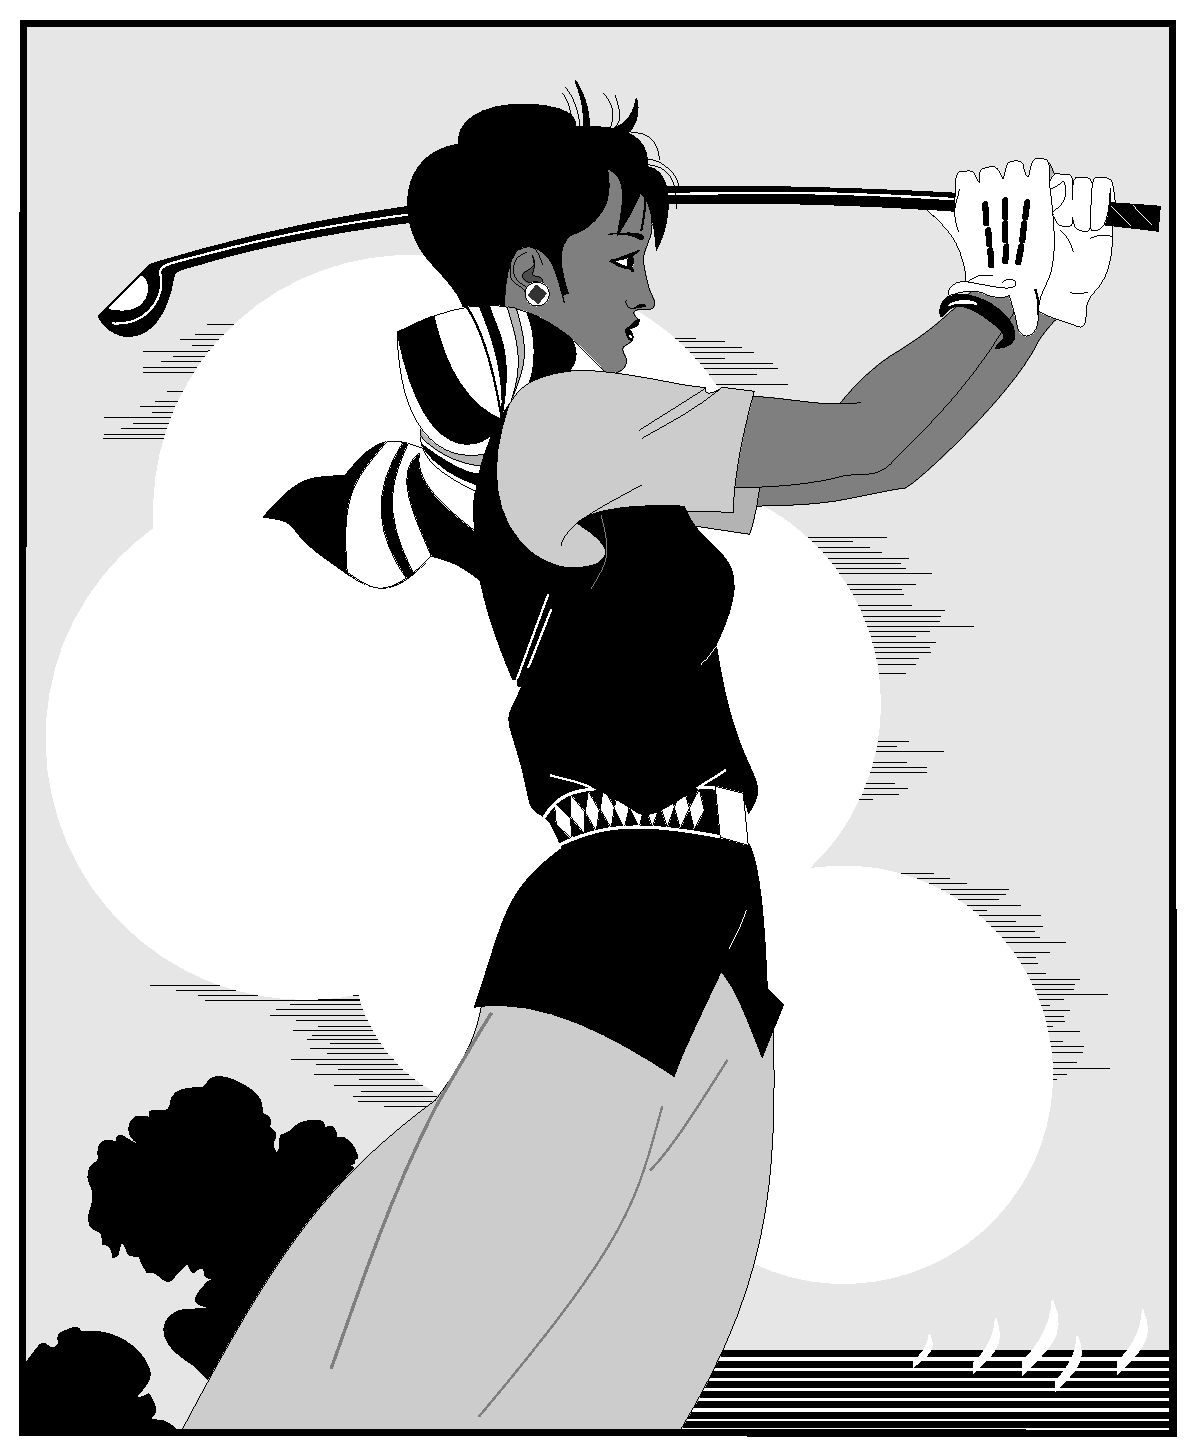
\includegraphics[width = 0.4\textwidth]{golfer}
% \bicaption[golfer1]{}{注意图中文字尽量用五号字
% }{Fig.$\!$}{The person playing golf}
% \end{figure}
% \end{latex}
% 单张单图题的格式如下,
% \begin{latex}
% \begin{figure}[h]
% \centering
% 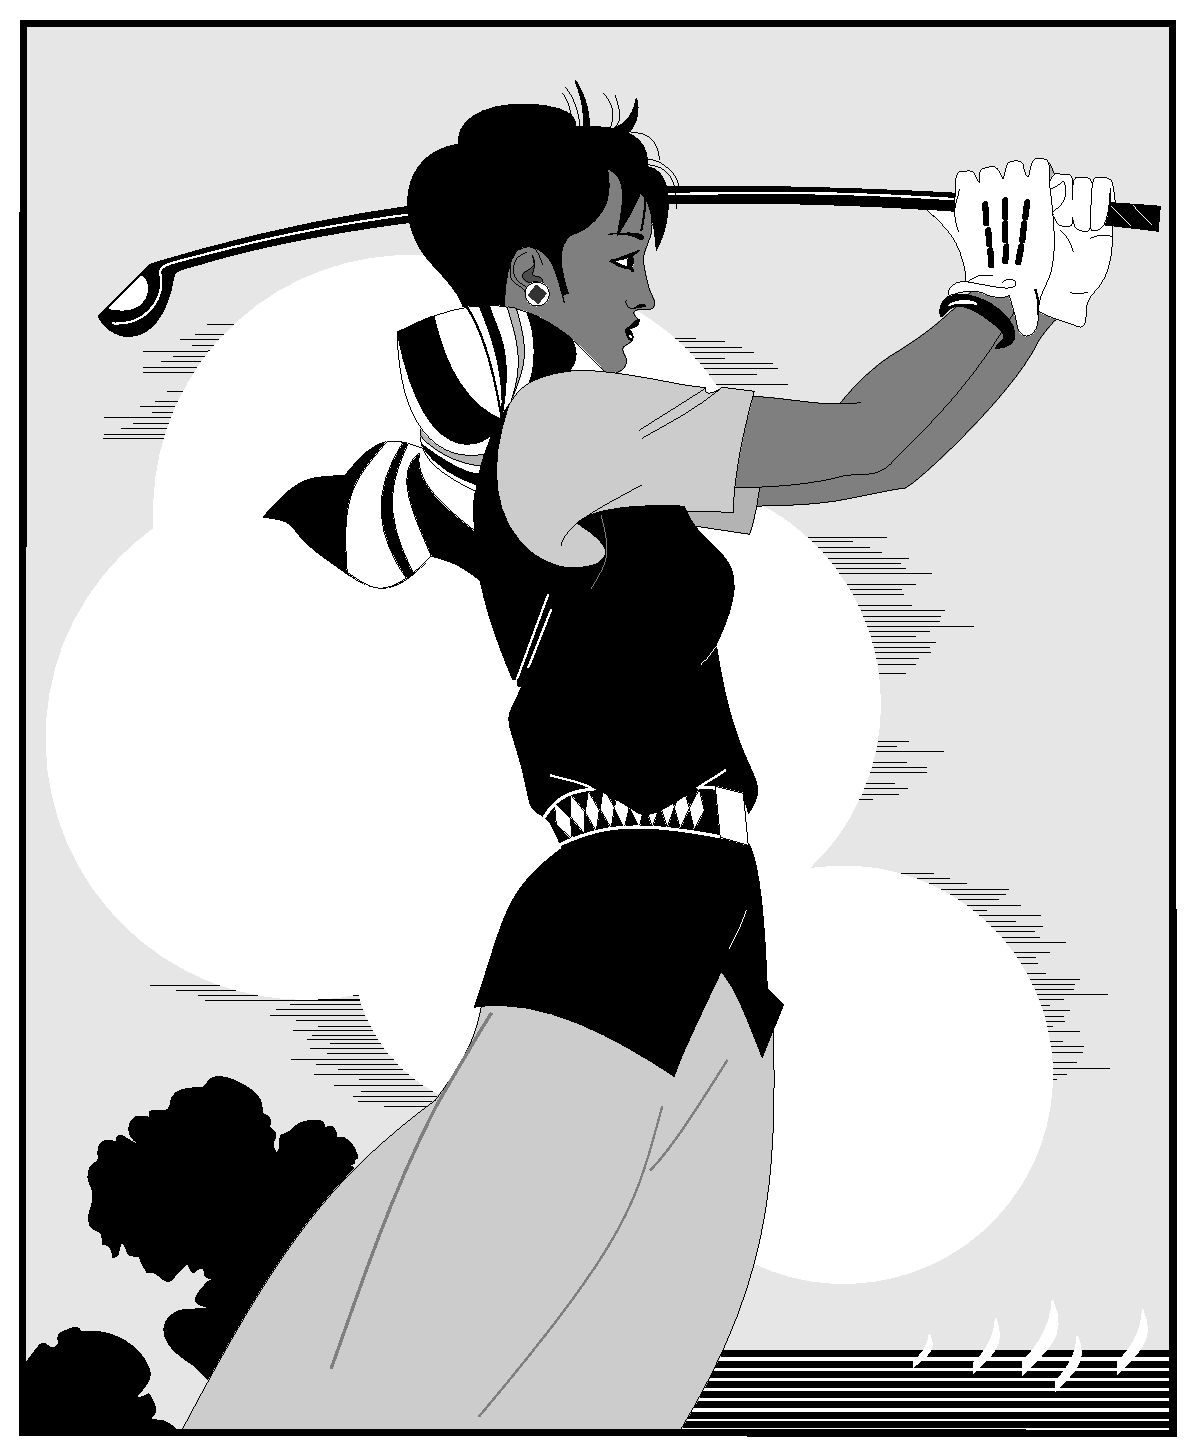
\includegraphics[width = 0.4\textwidth]{golfer}
% \caption{注意图中文字字号尽量用五号字}
% \end{figure}
% \end{latex}
% 并排图例。
% \begin{latex}
% \begin{figure}[htbp]
% \centering
% \begin{minipage}{0.4\textwidth}
% \centering
% 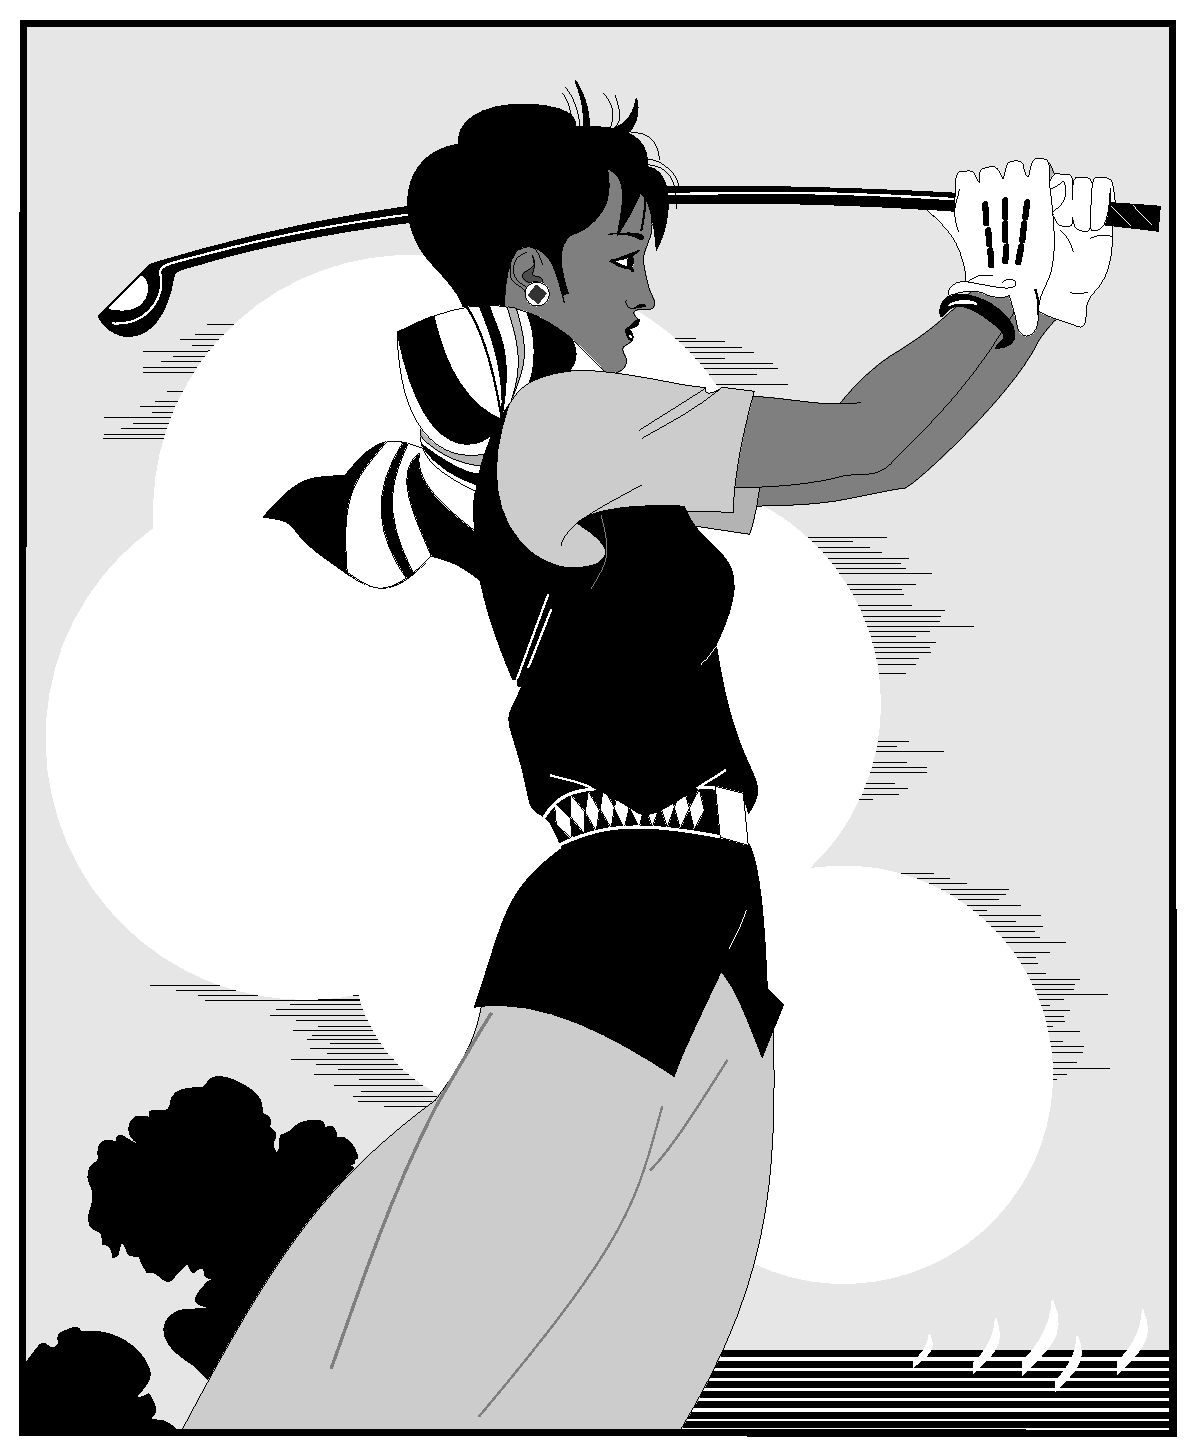
\includegraphics[width=\textwidth]{golfer}
% \bicaption[golfer2]{}{打高尔夫球的人}{Fig.$\!$}{The person playing golf}
% \end{minipage}
% \begin{minipage}{0.4\textwidth}
% \centering
% 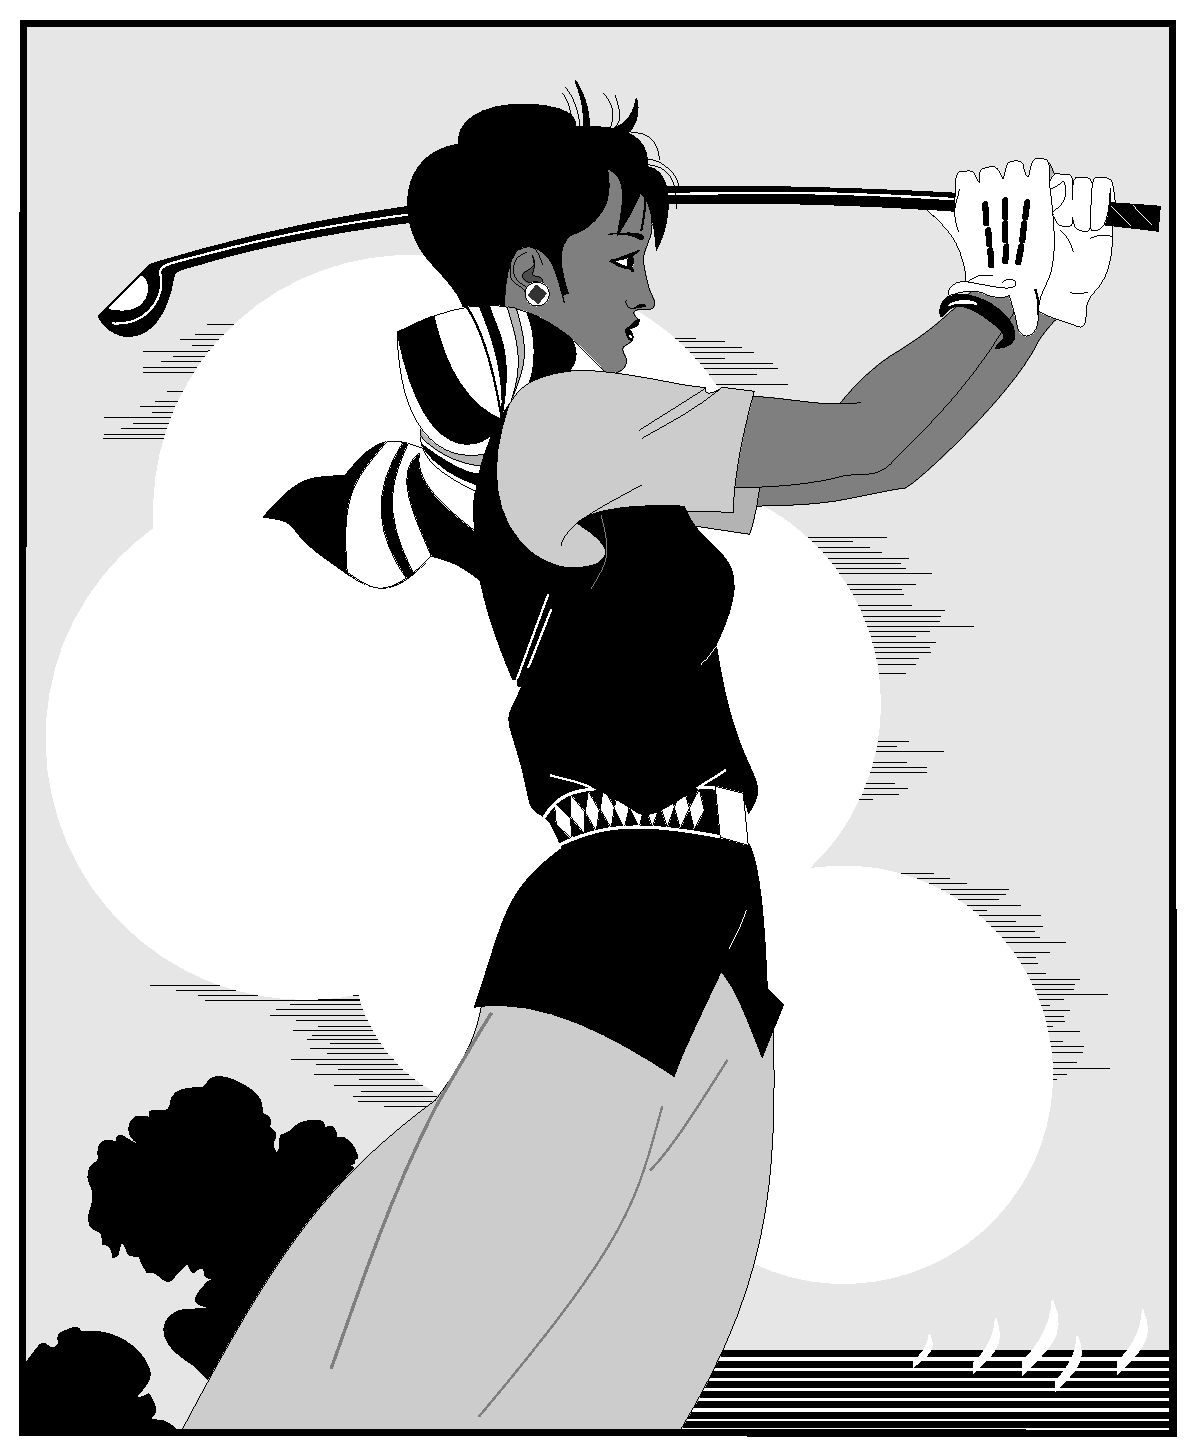
\includegraphics[width=\textwidth]{golfer}
% \bicaption[golfer3]{}{打高尔夫球的人}{Fig.$\!$}{The person playing golf}
% \end{minipage}
% \end{figure}
% \end{latex}
% 子图图例。
% \begin{latex}
% \begin{figure}[htbp]
% \centering
% \subfigure{\label{golfer41}}\addtocounter{subfigure}{-2}
% \subfigure[The person playing golf]{\subfigure[打高尔夫球的人~1]{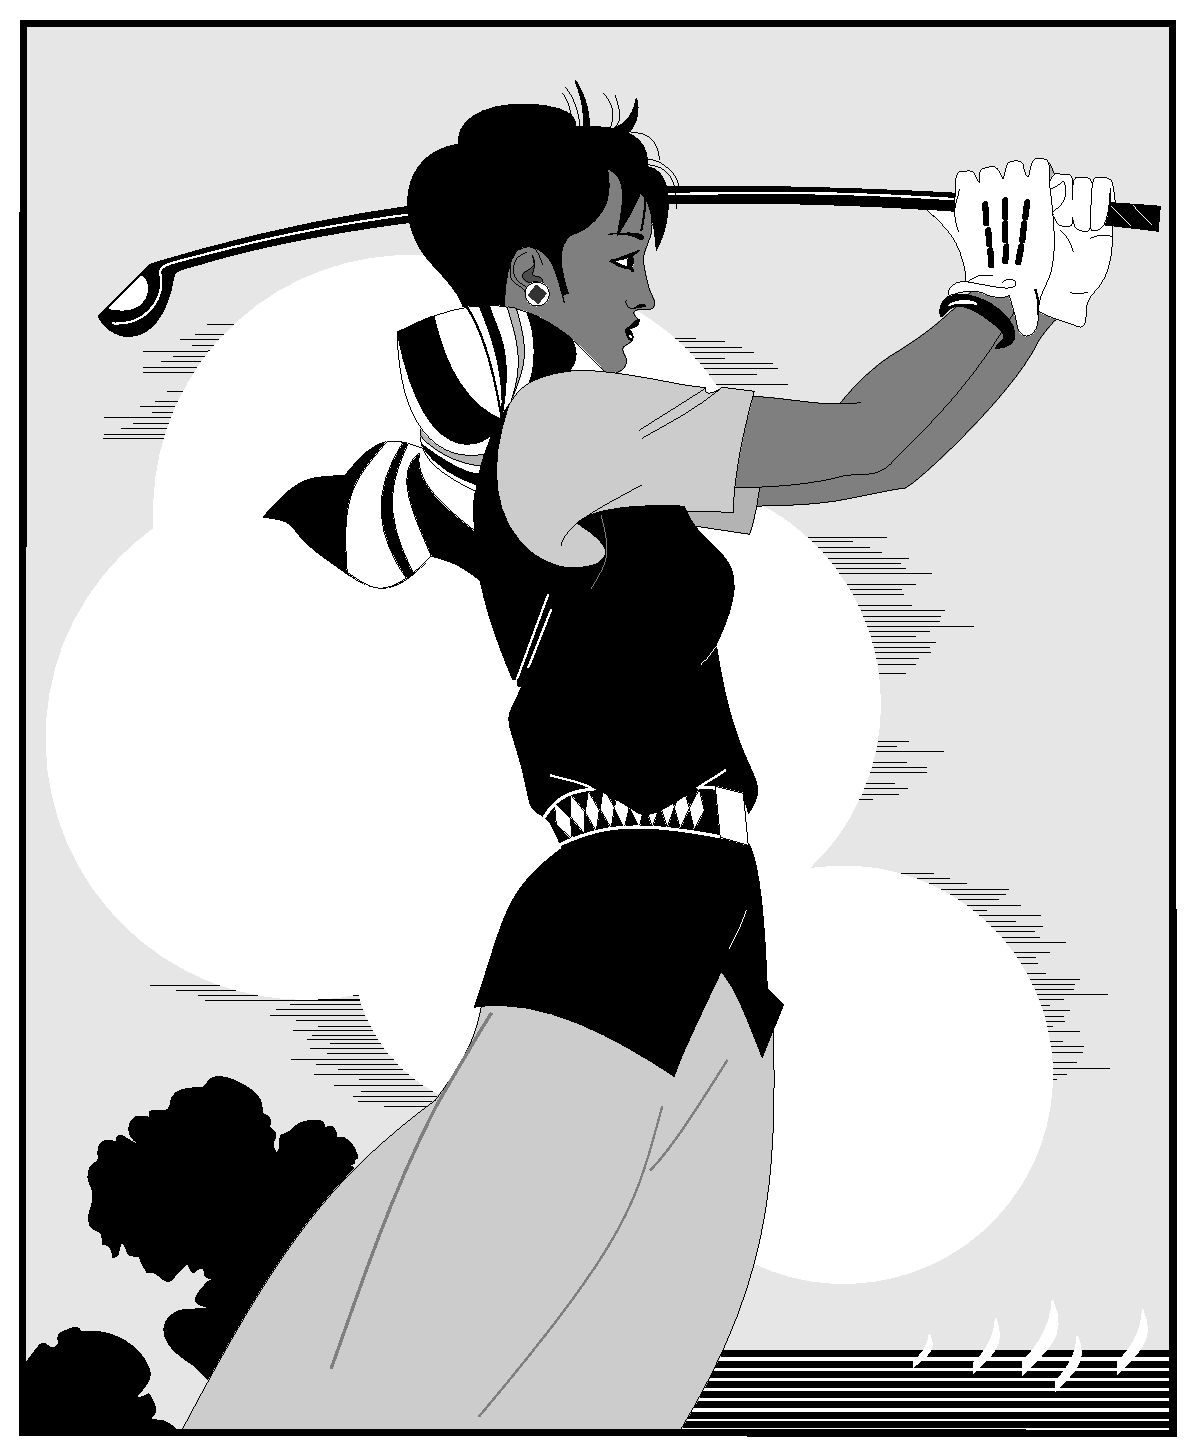
\includegraphics[width=0.4\textwidth]{golfer}}}
% \subfigure{\label{golfer42}}\addtocounter{subfigure}{-2}
% \subfigure[The person playing golf]{\subfigure[打高尔夫球的人~2]{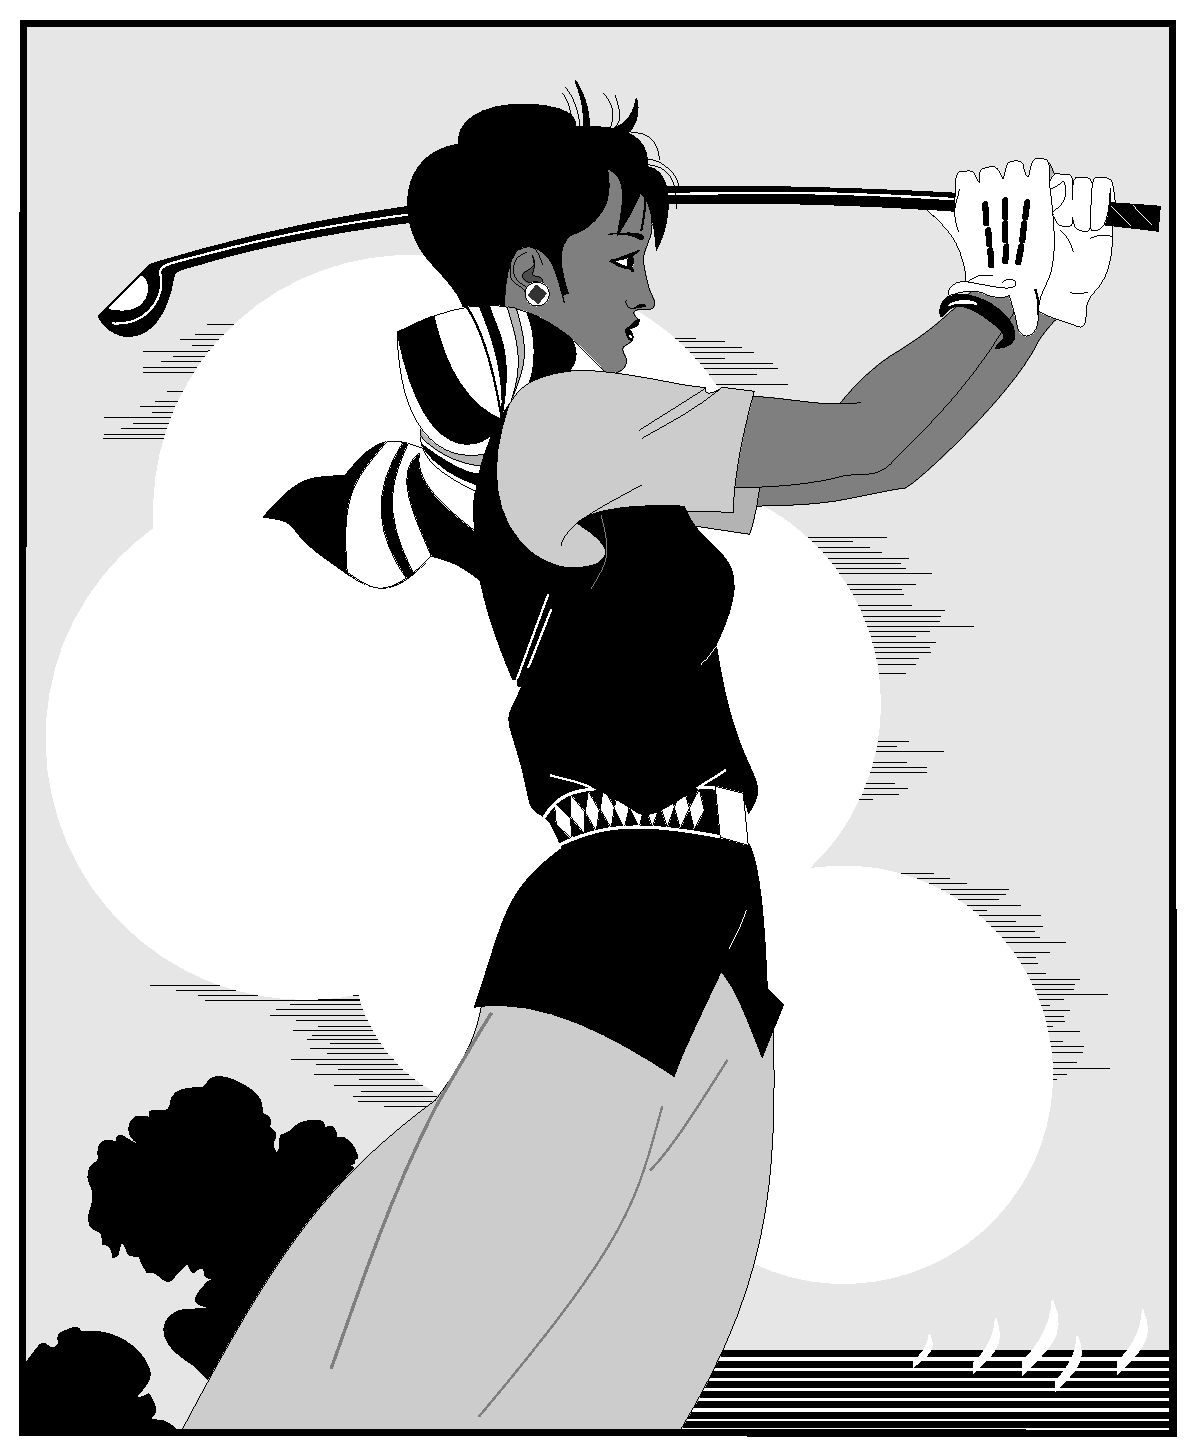
\includegraphics[width=0.4\textwidth]{golfer}}}
% \bicaption[golfer4]{}{打高尔夫球的人}{Fig.$\!$}{The person playing golf}
% \end{figure}
% \end{latex}
% 表格示例,表格中的字体是可以自行调整的。
% \begin{latex}
% \begin{table}[htbp]
% \bicaption[table1]{}{符合研究生院绘图规范的表格}{Table$\!$}{Table in agreement of the standard from graduate school}
% \vspace{0.5em}\centering\wuhao
% \begin{tabular}{ccccc}
% \toprule[1.5pt]
% $D$(in) & $P_u$(lbs) & $u_u$(in) & $\beta$ & $G_f$(psi.in)\\
% \midrule[1pt]
%  5 & 269.8 & 0.000674 & 1.79 & 0.04089\\
% 10 & 421.0 & 0.001035 & 3.59 & 0.04089\\
% 20 & 640.2 & 0.001565 & 7.18 & 0.04089\\
% \bottomrule[1.5pt]
% \end{tabular}
% \end{table}
% \end{latex}
% 因为长表格不是浮动体,不会自动调整位置、也不会自动调整字体大小,一切都要手动设
% 置。特别繁琐。
% \begin{latex}
% \ltfontsize{\dawu[1.667]} %设置表格内字体行间距
% \dawu[1.667]\begin{longtable}{ccc} % 注意此处设置的是表格线距离
% \longbionenumcaption{}{{\wuhao 中国省级行政单位一览 %此处要添加字体设置
% }\label{table2}}{Table$\!$}{}{{\wuhao Overview of the provincial administrative
% unit of China}}{-0.5em}{3.15bp}\\ %注意后两个参数分别是中英标题间距、标题和表格的间距。
% %\caption{\wuhao 中国省级行政单位一览}\\[1em] %注意此处是标题和表格间距,这行
% %是单语标题
% \toprule[1.5pt] 名称 & 简称 & 省会或首府  \\ \midrule[1pt]
% \endfirsthead
% \multicolumn{3}{r}{表~\thetable(续表)}\vspace{0.5em}\\
% \toprule[1.5pt] 名称 & 简称 & 省会或首府  \\ \midrule[1pt]
% \endhead
% \bottomrule[1.5pt]
% \endfoot
% 北京市 & 京 & 北京\\
% 天津市 & 津 & 天津\\
% 河北省 & 冀 & 石家庄市\\
% 山西省 & 晋 & 太原市\\
% 内蒙古自治区 & 蒙 & 呼和浩特市\\
% 辽宁省 & 辽 & 沈阳市\\
% 吉林省 & 吉 & 长春市\\
% 黑龙江省 & 黑 & 哈尔滨市\\
% 上海市 & 沪/申 & 上海\\
% 江苏省 & 苏 & 南京市\\
% 浙江省 & 浙 & 杭州市\\
% 安徽省 & 皖 & 合肥市\\
% 福建省 & 闽 & 福州市\\
% 江西省 & 赣 & 南昌市\\
% 山东省 & 鲁 & 济南市\\
% 河南省 & 豫 & 郑州市\\
% 湖北省 & 鄂 & 武汉市\\
% 湖南省 & 湘 & 长沙市\\
% 广东省 & 粤 & 广州市\\
% 广西壮族自治区 & 桂 & 南宁市\\
% 海南省 & 琼 & 海口市\\
% 重庆市 & 渝 & 重庆\\
% 四川省 & 川/蜀 & 成都市\\
% 贵州省 & 黔/贵 & 贵阳市\\
% 云南省 & 云/滇 & 昆明市\\
% 西藏自治区 & 藏 & 拉萨市\\
% 陕西省 & 陕/秦 & 西安市\\
% 甘肃省 & 甘/陇 & 兰州市\\
% 青海省 & 青 & 西宁市\\
% 宁夏回族自治区 & 宁 & 银川市\\
% 新疆维吾尔自治区 & 新 & 乌鲁木齐市\\
% 香港特别行政区 & 港 & 香港\\
% 澳门特别行政区 & 澳 & 澳门\\
% 台湾省 & 台 & 台北市\\
% \end{longtable}\normalsize %注意这里要恢复正常字体
% \end{latex}
% \subsubsection{公式}
% 公式不做介绍,与正常用法一致。
% \subsubsection{数学环境}
% \label{sec:math}
% \hithesis\ 定义了常用的数学环境:
%
% \begin{center}
% \begin{tabular}{*{7}{l}}\toprule
%   axiom & theorem & definition & proposition & lemma & conjecture &\\
%   公理 & 定理 & 定义 & 命题 & 引理 & 猜想 &\\\midrule
%   proof & corollary & example & exercise & assumption & remark & problem \\
%   证明 & 推论 & 例子& 练习 & 假设 & 注释 & 问题\\\bottomrule
% \end{tabular}
% \end{center}
%
% 比如:
% \begin{latex}
% \begin{definition}
%   道千乘之国,敬事而信,节用而爱人,使民以时。
% \end{definition}
% \end{latex}
% 产生(自动编号):
% \medskip
%
% \noindent\framebox[\linewidth][l]{{\heiti 定义~1.1~~~} % {道千乘之国,敬事而信,节用而爱人,使民以时。}}
%
% \smallskip
% 列举出来的数学环境毕竟是有限的,如果想用\emph{胡说}这样的数学环境,那么可以定义:
% \begin{latex}
% \newtheorem{nonsense}{胡说}[chapter]
% \end{latex}
%
% 然后这样使用:
% \begin{latex}
% \begin{nonsense}
%   契丹武士要来中原夺武林秘笈。—— 慕容博
% \end{nonsense}
% \end{latex}
% 产生(自动编号):
%
% \medskip
% \noindent\framebox[\linewidth][l]{{\heiti 胡说~1.1~~~} % {契丹武士要来中原夺武林秘笈。—— 慕容博}}
% \subsubsection{算法}
% 我工算法不在规范中要求且一千个评审老师有一千个算法格式喜好。详见
% \href{https://github.com/PlutoThesis/PlutoThesis#%E6%B2%A1%E6%9C%89%E6%98%8E%E7%A1%AE%E8%A6%81%E6%B1%82%E7%9A%84%E6%A0%BC%E5%BC%8F}{PlutoThesis}
% 中的各个实验室算法喜好举例。在此多说无益。
% \subsubsection{引用参考文献}
% \DescribeMacro{\inlinecite}
% 学校要求的参考文献引用有两种模式:(1)上标模式。比如``同样的工作有很
% 多$^{[1,2]}$\ldots''。(2)正文模式。比如``文[3] 中详细说明了\ldots''。其中上标
% 模式使用远比正文模式频繁,所以为了符合使用习惯,上标模式仍然用常规
% 的 \cs{cite}\marg{key},而 \cs{inlinecite}\marg{key} 则用来生成正文模式。
%
% 关于参考文献模板推荐使用 \BibTeX,关于中文参考文献需要额外增加一个 Entry:
% \texttt{lang},将其设置为 \texttt{zh} 用来指示此参考文献为中文,以
% 便 \file{hithesis.bst} 处理。如:
% \begin{latex}
% @INPROCEEDINGS{cnproceed,
%   author    = {王重阳 and 黄药师 and 欧阳峰 and 洪七公 and 段皇帝},
%   title     = {武林高手从入门到精通},
%   booktitle = {第~$N$~次华山论剑},
%   year      = 2006,
%   address   = {西安, 中国},
%   month     = sep,
%   lang      = "zh",
% }
%
% @ARTICLE{cnarticle,
%   AUTHOR  = "贾宝玉 and 林黛玉 and 薛宝钗 and 贾探春",
%   TITLE   = "论刘姥姥食量大如牛之现实意义",
%   JOURNAL = "红楼梦杂谈",
%   PAGES   = "260--266",
%   VOLUME  = "224",
%   YEAR    = "1800",
%   LANG    = "zh",
% }
% \end{latex}
%
% 注意如果不需要引用参考文献,请删除 \file{main.tex} 中 \cs{bibliography} 开头的两行,
% 以避免可能的编译错误。
%
% \subsubsection{列表环境}
% \DescribeEnv{itemize}
% \DescribeEnv{enumerate}
% \DescribeEnv{description}
% 为了适合中文习惯,模板将这三个常用的列表环境用 \pkg{enumitem} 进行了纵向间距压
% 缩。一方面清除了多余空间,另一方面用户可以自己指定列表环境的样式(如标签符号,
% 缩进等)。细节请参看 \pkg{enumitem} 文档,此处不再赘述。
% \subsection{后文}
%
% \subsubsection{结论}
% \DescribeEnv{conclusion}
% 结论之后为后文内容。
% \begin{latex}
% \begin{conclusions}
%
% 学位论文的结论作为论文正文的最后一章单独排写,但不加章标题序号。
%
% 结论应是作者在学位论文研究过程中所取得的创新性成果的概要总结,不能与摘要混为一
% 谈。博士学位论文结论应包括论文的主要结果、创新点、展望三部分,在结论中应概括论
% 文的核心观点,明确、客观地指出本研究内容的创新性成果(含新见解、新观点、方法创
% 新、技术创新、理论创新),并指出今后进一步在本研究方向进行研究工作的展望与设想
% 。对所取得的创新性成果应注意从定性和定量两方面给出科学、准确的评价,分(1)、
% (2)、(3)…条列出,宜用“提出了”、“建立了”等词叙述。
%
% \end{conclusions}
% \end{latex}
%
% \subsubsection{参考文献}
% 在后文中的参考文献是自动生成的,不需要用户干预,具体命令在\file{main.tex}中有
% 示例。
%
% \subsubsection{附录}
% \DescribeEnv{appendix}
% 所有的附录都插到这里来。因为附录会更改默认的 chapter 属性,而后面的{\heiti 个人简
%   历}又需要恢复,所以实现为环境可以保证全局的属性不受影响。
% \begin{latex}
% \begin{appendix}
% % -*-coding: utf-8 -*-
%%%%%%%%%%%%%%%%%%%%%%%%%%%%%%%%%%%%%%%%%%%%%%%%%%%%%%%%%
\chapter{带章节的附录}[Full Appendix]%
完整的附录内容,包含章节,公式,图表等

%%%%%%%%%%%%%%%%%%%%%%%%%%%%%%%%%%%%%%%%%%%%%%%%%%%%%%%%%
\section{附录节的内容}[Section in Appendix]
这是附录的节的内容

附录中图的示例:
\begin{figure}[htbp]
\centering
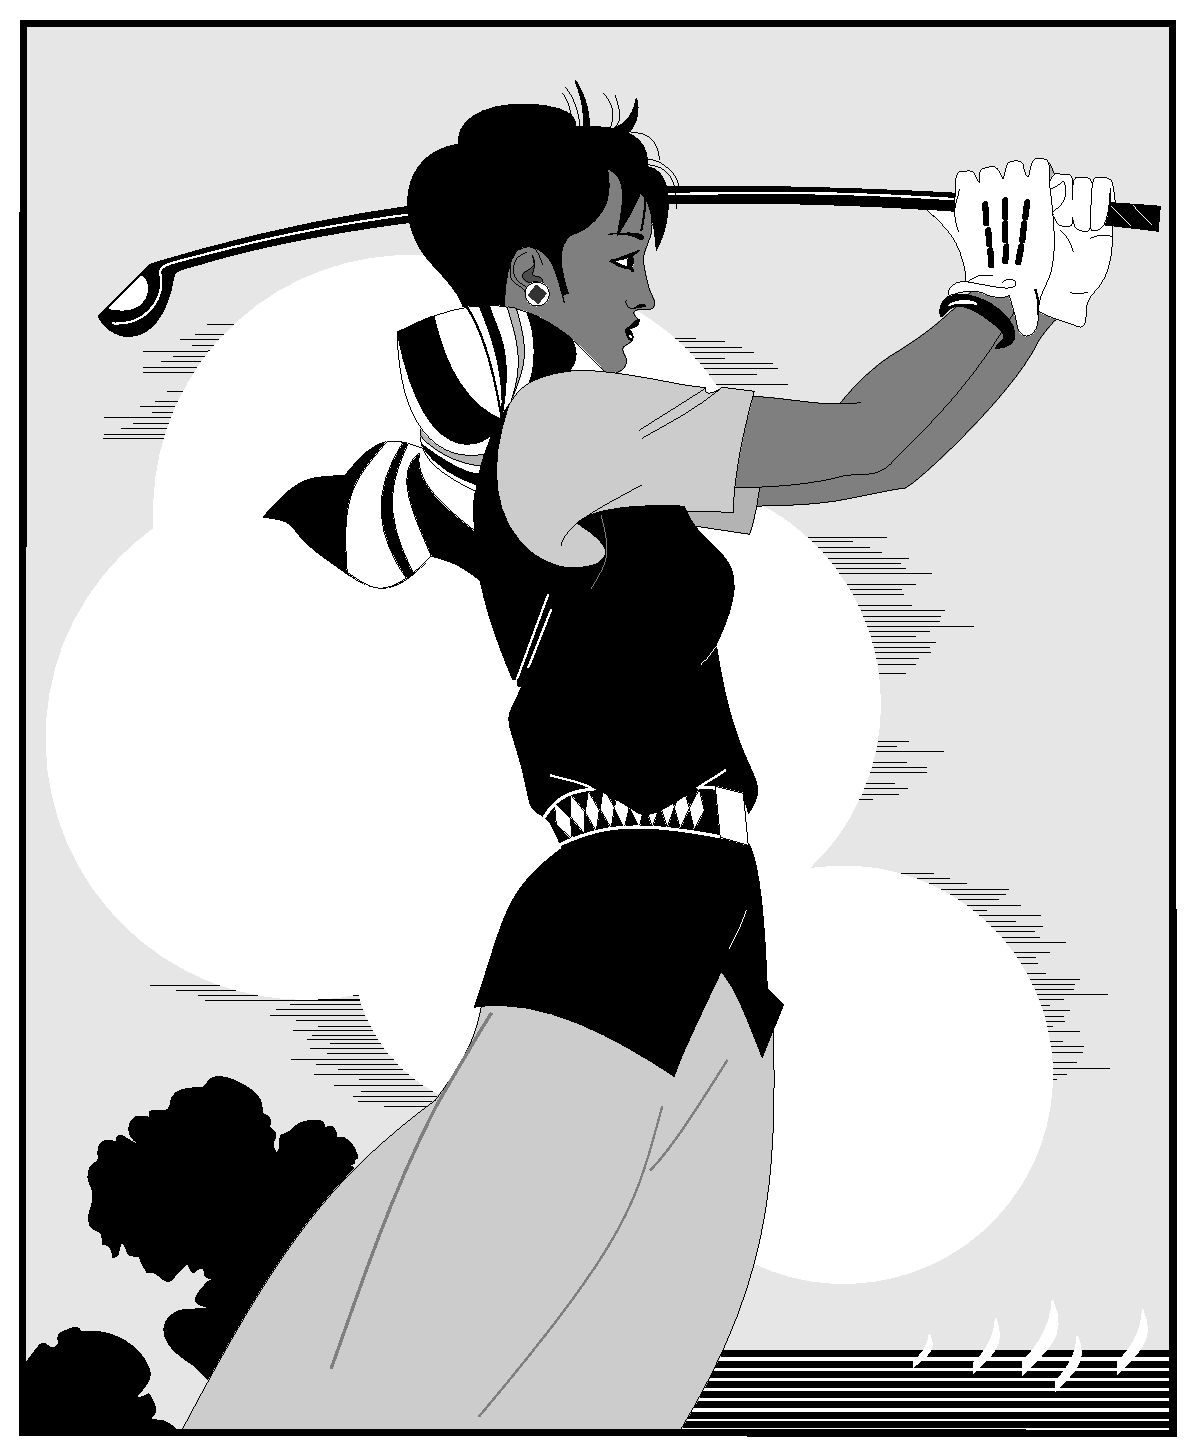
\includegraphics[width = 0.4\textwidth]{golfer}
%\bicaption[golfer5]{}{\xiaosi[0]打高尔夫球的人}{Fig.$\!$}{The person playing golf}\vspace{-1em}
\caption{\xiaosi[0]打高尔夫球的人}
\end{figure}

附录中公式的示例:
\begin{align}
a & = b \times c \\
E & = m c^2
\label{eq}
\end{align}

\chapter{这个星球上最好的免费Linux软件列表}[List of the Best Linux Software in our Planet]
\section{系统}

\href{http://fvwm.org/}{FVWM 自从上世纪诞生以来,此星球最强大的窗口管理器。}
推荐基于FVWM的桌面设计hifvwm:\href{https://github.com/dustincys/hifvwm}{https://github.com/dustincys/hifvwm}。

\subsection{hifvwm的优点}

\begin{enumerate}
	\item 即使打开上百个窗口也不会“蒙圈”。计算机性能越来越强大,窗口任务的管理必须要升级到打怪兽级别。
	\item 自动同步Bing搜索主页的壁纸。每次电脑开机,午夜零点自动更新,用户
		也可以手动更新,从此审美再也不疲劳。
	\item 切换窗口自动聚焦到最上面的窗口。使用键盘快捷键切换窗口时候,减少
		操作过程,自动聚焦到目标窗口。这一特性是虚拟窗口必须的人性化设
		计。
	\item 类似window右下角的功能的最小化窗口来显示桌面的功能此处类似
		win7/win10,实现在一个桌面之内操作多个任务。
	\item 任务栏结合标题栏。采用任务栏和标题栏结合,节省空间。
	\item 同类窗口切换。可以在同类窗口之内类似alt-tab的方式切换。
	\item ……
\end{enumerate}

\section{其他}

\href{https://github.com/goldendict/goldendict}{goldendict 星球最强大的桌面字典。}

\href{https://github.com/yarrick/iodine}{iodine,“HIT-WLAN + 锐捷”时代的福音。}

\href{http://www.aircrack-ng.org/}{aircrack,Wifi“安全性评估”工具。}

\href{https://www.ledger-cli.org/}{ledger,前“金融区块链”时代最好的复式记账系统。}

\href{https://orgmode.org/}{orgmode,最强大的笔记系统,从来没有之一。}

\href{https://www.jianguoyun.com/}{坚果云,国内一款支持WebDav的云盘系统,国内真正的云盘没有之一。}

\href{http://www.mutt.org/}{mutt, ``All mail clients suck. This one just sucks less.''}

\section{vim}
实现中英文每一句一行,以及实现每一句折叠断行的简单正则式,tex源码更加乖乖。
\begin{lstlisting}
vnoremap <leader>fae J:s/[.!?]\zs\s\+/\="\r".matchstr(getline('.'), '^\s*')/g<CR>
vnoremap <leader>fac J:s/[。!?]/\=submatch(0)."\n".matchstr(getline('.'), '^\s*')/g<CR>
vnoremap <leader>fle :!fmt -80 -s<CR>
\end{lstlisting}

% \end{appendix}
% \end{latex}
%
% \subsubsection{所发表文章}
% \DescribeEnv{publication}
% 虽然在\PGR\UGR\ 中都没有明确规定此处的格式,但按照旧模板PlutoThesis,此处格式
% 非常复杂。此处仍然使用旧模板中的设置方法。
% \begin{latex}
% \begin{publication}
% \noindent\textbf{(一)发表的学术论文}
% \begin{publist}
% \item	XXX,XXX. Static Oxidation Model of Al-Mg/C Dissipation Thermal Protection Materials[J]. Rare Metal Materials and Engineering, 2010, 39(Suppl. 1): 520-524.(SCI~收录,IDS号为~669JS,IF=0.16)
% \item XXX,XXX. 精密超声振动切削单晶铜的计算机仿真研究[J]. 系统仿真学报,2007,19(4):738-741,753.(EI~收录号:20071310514841)
% \item XXX,XXX. 局部多孔质气体静压轴向轴承静态特性的数值求解[J]. 摩擦学学报,2007(1):68-72.(EI~收录号:20071510544816)
% \item XXX,XXX. 硬脆光学晶体材料超精密切削理论研究综述[J]. 机械工程学报,2003,39(8):15-22.(EI~收录号:2004088028875)
% \item XXX,XXX. 基于遗传算法的超精密切削加工表面粗糙度预测模型的参数辨识以及切削参数优化[J]. 机械工程学报,2005,41(11):158-162.(EI~收录号:2006039650087)
% \item XXX,XXX. Discrete Sliding Mode Cintrok with Fuzzy Adaptive Reaching Law on 6-PEES Parallel Robot[C]. Intelligent System Design and Applications, Jinan, 2006: 649-652.(EI~收录号:20073210746529)
% \end{publist}
%
% \noindent\textbf{(二)申请及已获得的专利(无专利时此项不必列出)}
% \begin{publist}
% \item XXX,XXX. 一种温热外敷药制备方案:中国,88105607.3[P]. 1989-07-26.
% \end{publist}
%
% \noindent\textbf{(三)参与的科研项目及获奖情况}
% \begin{publist}
% \item	XXX,XXX. XX~气体静压轴承技术研究, XX~省自然科学基金项目.课题编号:XXXX.
% \item XXX,XXX. XX~静载下预应力混凝土房屋结构设计统一理论. 黑江省科学技术二等奖, 2007.
% \end{publist}
% %\vfill
% %\hangafter=1\hangindent=2em\noindent
% %\setlength{\parindent}{2em}
% \end{publication}
% \end{latex}
%
% \subsubsection{索引}
% \DescribeEnv{ceindex}
% 我工要求中英文双语索引。后文中的自动索引实际上不需要用户干预。
%\begin{latex}
% \begin{ceindex}
%   %如果想要手动加索引,注释掉以下这一样,用wordlist环境
% \printsubindex*
% \end{ceindex}
%\end{latex}
% 手工添加索引的方法不推荐,模板中将去除该功能。
% \subsubsection{授权}
% \DescribeMacro{\authorization}
% 授权页中的签名和日期是需要手写,不需要人工干预。具体示例在\file{main.tex}中。
%\begin{latex}
% \authorization %授权
% %\authorization[saomiao.pdf] %添加扫描页的命令,与上互斥
%\end{latex}
%
% \subsubsection{致谢声明}
% \DescribeEnv{acknowledgement}
% 把致谢做成一个环境更好一些,直接往里面写感谢的话就可以啦!
%
% \begin{latex}
% \begin{acknowledgement}
%   …
%   感谢\hit\LaTeX\ 论文模板\hithesis\ !
% \end{acknowledgement}
% \end{latex}
%
%
% \subsubsection{简历}
% \DescribeEnv{resume}
% 个人简历。
% 实际上,致谢和个人简历是自由发挥的地区,字体,文体,格式,内容,完全自己决定。
% \begin{latex}
% \begin{resume}
% XXXX~年~XX~月~XX~日出生于~XXXX。
%
% XXXX~年~XX~月考入~XX~大学~XX~院(系)XX~专业,XXXX~年~XX~月本科毕业并获得~XX~学学士学位。
%
% XXXX~年~XX~月------XXXX~年~XX~月在~XX~大学~XX~院(系)XX~学科学习并获得~XX~学硕士学位。
%
% XXXX~年~XX~月------XXXX~年~XX~月在~XX~大学~XX~院(系)XX~学科学习并获得~XX~学博士学位。
%
% 获奖情况:如获三好学生、优秀团干部、X~奖学金等(不含科研学术获奖)。
%
% 工作经历:
% \end{resume}
% \end{latex}
%
% \subsection{其它}
% 模板的配置文件 \file{hithesis.cfg} 中定义了很多固定词汇,一般无须修改。如果有特殊需求,
% 推荐在导言区使用 \cs{renewcommand}。
%
%
% \subsection{捐助}
% \changes{v1.0.1}{2017/08/27}{添加了捐助、矢量化本科论文模板的图片logo}
% 各位刀客和大侠如用的嗨,要解囊相助,请微信或支付宝参照图
% ~\ref{wct5}-\ref{zfb}~中提示操作(二维码被矢量化后之后去
% 除了头像等冗余无用的部分~)。
% \begin{figure}[h]
% \centering\includegraphics[width=0.5\textwidth]{wct5.eps}
% \caption{如果用的嗨,微信扫码捐助5元~~}
% \label{wct5}
% \end{figure}
% \begin{figure}[h]
% \centering\includegraphics[width=0.5\textwidth]{wct10.eps}
% \caption{如果用的非常嗨,微信扫码捐助10元~~}
% \label{wct10}
% \end{figure}
% \begin{figure}[h]
% \centering\includegraphics[width=0.5\textwidth]{wct1.eps}
% \caption{那个,看在熬夜写代码的份上,微信扫码捐助1元吧~~}
% \label{wct1}
% \end{figure}
% \begin{figure}[h]
% \centering\includegraphics[width=0.5\textwidth]{zfb.eps}
% \caption{支付宝不限额度}
% \label{zfb}
% \end{figure}
%
% \StopEventually{\PrintChanges\PrintIndex}
% \clearpage
%
% \section{实现细节}
%
% \subsection{基本信息}
%    \begin{macrocode}
%<cls>\NeedsTeXFormat{LaTeX2e}[1999/12/01]
%<cls>\ProvidesClass{hithesis}
%<cfg>\ProvidesFile{hithesis.cfg}
%<cls|cfg>[2018/12/05 2.0.6 Harbin Institute of Technology Thesis Template]
%    \end{macrocode}
%
% \subsection{定义选项}
% \label{sec:defoption}
%    \begin{macrocode}
%<*cls>
\RequirePackage{ifthen}
\RequirePackage{kvoptions}
\SetupKeyvalOptions{
  family=hit,
  prefix=hit@,
  setkeys=\kvsetkeys}
\newif\ifhit@bachelor
\newif\ifhit@master
\newif\ifhit@doctor
\define@key{hit}{type}{%
  \hit@bachelorfalse
  \hit@masterfalse
  \hit@doctorfalse
  \expandafter\csname hit@#1true\endcsname}
%    \end{macrocode}
%	定义stage项,区分开题、中期,默认false,为毕业论文,empty为空-去掉页眉 _added by t
%    \begin{macrocode}
\newif\ifhit@kaiti
\newif\ifhit@zhongqi
\define@key{hit}{stage}{%
  \hit@kaitifalse
  \hit@zhongqifalse
  \expandafter\csname hit@#1true\endcsname}
%    \end{macrocode}
%    设置版芯,由于窝工版芯歧义。
% \changes{v2.0.0}{2018/6/14}{此处添加geometry选项}
%    \begin{macrocode}
\newif\ifhit@geometrynewone
\newif\ifhit@geometrynewtwo
\define@key{hit}{newgeometry}{%
  \hit@geometrynewonefalse
  \hit@geometrynewtwofalse
  \expandafter\csname hit@geometrynew#1true\endcsname}
%    \end{macrocode}
% 目录中英文是否用 Arial 字体(默认关闭)。
%    \begin{macrocode}
\DeclareBoolOption[false]{arialtoc}
%    \end{macrocode}
% 章节标题中的英文是否用 Arial 字体(默认打开)。
%    \begin{macrocode}
\DeclareBoolOption[false]{arialtitle}
%    \end{macrocode}
% \changes{v1.0.3}{2017/08/29}{默认开启raggedbottom}
% \option{raggedbottom} 选项(默认开启)。如果不开启这个选项,会出现一页中尽量上
% 下对齐,段的间距大。如果开启,尽量使段间距保持一致,页面底部出现空白。
%    \begin{macrocode}
\DeclareBoolOption[true]{raggedbottom}
%    \end{macrocode}
% 在脚注标记中使用 \pkg{pifont} 的带圈数字(默认关闭)。
%    \begin{macrocode}
\DeclareBoolOption[false]{pifootnote}
%    \end{macrocode}
% 字体间距设置(默认关闭)。
%    \begin{macrocode}
\DeclareBoolOption[false]{glue}
%    \end{macrocode}
% 文科生四级目录设置(默认关闭)。
%    \begin{macrocode}
\DeclareBoolOption[false]{tocfour}
%    \end{macrocode}
% 目录中“目录”位置是否空行(默认开启)。
%    \begin{macrocode}
\DeclareBoolOption[true]{tocblank}
%    \end{macrocode}
% 章标题是否悬挂居中(默认开启)
%    \begin{macrocode}
\DeclareBoolOption[true]{chapterhang}
%    \end{macrocode}
% 是否是全日制学生(默认是)。
%    \begin{macrocode}
\DeclareBoolOption[true]{fulltime}
%    \end{macrocode}
% 是否有子标题(默认是)。
%    \begin{macrocode}
\DeclareBoolOption[false]{subtitle}
%    \end{macrocode}
% 是否开启debug模式(默认否)。如果开启,载入显示行号等的包,只为开发调试用。
%    \begin{macrocode}
\DeclareBoolOption[false]{debug}
%    \end{macrocode}
% \changes{v2.0.0}{2018/6/14}{此处删除newgeometry选项}
% 是否使用右开页(默认否)。
%    \begin{macrocode}
\DeclareBoolOption[false]{openright}
%    \end{macrocode}
% 图题和标题最后一行是否居中对其(默认是,非规范要求)。
% \changes{v1.0.6}{2017/10/25}{此处更改了选项的名称}
%    \begin{macrocode}
\DeclareBoolOption[false]{capcenterlast}
%    \end{macrocode}
% 子图图题和标题最后一行是否居中对其(默认是,非规范要求)。
% \changes{v1.0.6}{2017/10/25}{此处添加子图最后一行图题是否居中选项}
%    \begin{macrocode}
\DeclareBoolOption[false]{subcapcenterlast}
%    \end{macrocode}
% 中文目录中Abstract是否均为大写
% \changes{v1.0.13}{2018/4/5}{此处添加中文目录中Abstract是否均为大写选项}
%    \begin{macrocode}
\DeclareBoolOption[false]{absupper}
%    \end{macrocode}
%    此处添加控制本科论文的页码横线选项
% \changes{v1.0.15}{2018/06/05}{添加控制本科论文的页码横线选项}
%    \begin{macrocode}
\DeclareBoolOption[false]{bsmainpagenumberline}
\DeclareBoolOption[false]{bsfrontpagenumberline}
\DeclareBoolOption[true]{bsheadrule}
%    \end{macrocode}
%    数学字体是否使用新罗马
% \changes{v2.0.5}{2018/12/05}{添加数学字体开关}
%    \begin{macrocode}
\DeclareBoolOption[true]{newtxmath}
%    \end{macrocode}
%    此处应广大刀客要求添加一参考文献分割开关
% \changes{v2.0.3}{2018/10/08}{添加参考文献分割开关}
%    \begin{macrocode}
\DeclareBoolOption[false]{splitbibitem}
%    \end{macrocode}
% 声明字体选项。
%    \begin{macrocode}
\DeclareBoolOption[false]{customheadfancy}
%	添加customheadfancy项,可以用来自定义页眉,默认false,暂时无用  _added by t
\DeclareBoolOption[false]{noheader}
%	添加noheader项,true时可以用来去掉页眉(开题、中期报告老师可能不让留页眉),默认false,保留页眉  _added by t
\DeclareStringOption{fontset}
%    \end{macrocode}
% 将其余选项默认传递给 \pkg{ctexbook}。
%    \begin{macrocode}
\DeclareDefaultOption{\PassOptionsToClass{\CurrentOption}{ctexbook}}
%    \end{macrocode}
% 解析用户传递过来的选项,并加载 \pkg{ctexbook}。
%    \begin{macrocode}
\ProcessKeyvalOptions*
%    \end{macrocode}
% 使用 \XeTeX\ 引擎时,\pkg{fontspec} 宏包会被 \pkg{xeCJK} 自动调用。传递
% 给 \pkg{fontspec} 宏包 \option{no-math} 选项,避免部分数学符号字体自动调整
% 为 CMR。其他引擎下没有这个问题,这一行会被无视。
%    \begin{macrocode}
\PassOptionsToPackage{no-math}{fontspec}
%    \end{macrocode}
% 载入单双面打印设置,本、硕单面,博士双面。
%    \begin{macrocode}
\ifhit@bachelor
\PassOptionsToClass{oneside}{book}
\fi
\ifhit@master
\PassOptionsToClass{oneside}{book}
\fi
\ifhit@doctor
\PassOptionsToClass{twoside}{book}
\fi
%    \end{macrocode}
% \changes{v1.0.2}{2017/08/27}{添加了思源字体说明}
% 设置字体。由于宋体没有粗体,且我工模板的标题要求使用粗宋体,于是面临CTeX的经典
% 的伪粗体bug:“首次出现伪粗体字体之后的正常字体无法复制”。但如果使用自带宋体的
% 思源字体,那么不必使用伪粗体。模板只给出了新windows字体的思源字体设置,且思源
% 字体版本为Adobe版。
%    \begin{macrocode}
\ifthenelse%
{\equal{\hit@fontset}{}}%
{%
  \PassOptionsToPackage{AutoFakeBold=2}{xeCJK}
}%
{%
  \ifthenelse%
  {\equal{\hit@fontset}{siyuan}}%
  {\relax}%
  {%
    \PassOptionsToPackage{AutoFakeBold=2}{xeCJK}
  }%
  \PassOptionsToClass{fontset=\hit@fontset}{ctexbook}
}%
%    \end{macrocode}
% 使用 \pkg{ctexbook} 类,优于调用 \pkg{ctex} 宏包。
%    \begin{macrocode}
\LoadClass[a4paper,openany,UTF8,zihao=-4,scheme=plain]{ctexbook}
%    \end{macrocode}
% 用户至少要提供一个选项,指定论文类型。
%    \begin{macrocode}
\ifhit@bachelor\relax\else
  \ifhit@master\relax\else
    \ifhit@doctor\relax\else
        \ClassError{hithesis}%
                   {Please specify thesis type in option: \MessageBreak
                    type=[bachelor | master | doctor]}{}
      \fi
  \fi
\fi
%    \end{macrocode}
%
% \subsection{装载宏包}
% \label{sec:loadpackage}
%
% 引用的宏包和相应的定义。
%    \begin{macrocode}
\RequirePackage{etoolbox}
\RequirePackage{ifxetex}
\ifxetex
\else
        \ClassError{hithesis}%
                   {Please use: \MessageBreak
                    xelatex}{}
\fi
\RequirePackage{xparse}
%    \end{macrocode}
%
% \AmSTeX\ 宏包,用来排出更加漂亮的公式。
%    \begin{macrocode}
\RequirePackage{amsmath}
%    \end{macrocode}
% \pkg{newtx} 设置 Times New Roman,Helvetica。
%    \begin{macrocode}
\RequirePackage[defaultsups]{newtxtext}
%    \end{macrocode}
% 添加数学字体开关
%    \begin{macrocode}
\ifhit@newtxmath
\RequirePackage{newtxmath}
\fi
%    \end{macrocode}
% \pkg{newtx} 的 Mono 字体虽然很好看,但在论文中不常见。学校虽未要求 Mono 字体,
% 还是选择常见的 Courier 字体。由于比较新的实现 \TeX\ Gyre Cursor 会修
% 改\cs{bfdefault},导致中文加粗出问题,所以选用标准 \pkg{courier}。
%    \begin{macrocode}
\RequirePackage{courier}
%    \end{macrocode}
% 图形支持宏包。
%    \begin{macrocode}
\RequirePackage{graphicx}
%    \end{macrocode}
% \pkg{pdfpages} 宏包便于我们插入扫描后的授权页和声明页 PDF 文档。
%    \begin{macrocode}
\RequirePackage{pdfpages}
\includepdfset{fitpaper=true}
%    \end{macrocode}
% 更好的列表环境。
%    \begin{macrocode}
\RequirePackage{enumitem}       %使用enumitem宏包,改变列表项的格式
\RequirePackage{environ}
%    \end{macrocode}
% 禁止 \LaTeX 自动调整多余的页面底部空白,并保持脚注仍然在底部。
% 脚注按页编号。
%    \begin{macrocode}
\ifhit@raggedbottom
  \RequirePackage[bottom,perpage,hang]{footmisc}
  \raggedbottom
\else
  \RequirePackage[perpage,hang]{footmisc}
\fi
%    \end{macrocode}
% 脚注格式。
%    \begin{macrocode}
\ifhit@pifootnote
  \RequirePackage{pifont}
\fi
%    \end{macrocode}
% 利用 \pkg{CJKfntef} 实现汉字的下划线和盒子内两段对齐,并可以避免
% \cs{makebox}\oarg{width}\oarg{s} 可能产生的 underful boxes。
%    \begin{macrocode}
\RequirePackage{CJKfntef}
%    \end{macrocode}
% 定理类环境宏包,其中 \pkg{amsmath} 选项用来兼容 \AmSTeX\ 的宏包
%    \begin{macrocode}
\RequirePackage[amsmath,thmmarks,hyperref]{ntheorem}
%    \end{macrocode}
% 表格控制
%    \begin{macrocode}
\RequirePackage{longtable}
%    \end{macrocode}
% 使用三线表:\cs{toprule},\cs{midrule},\cs{bottomrule}。
%    \begin{macrocode}
\RequirePackage{booktabs}
%    \end{macrocode}
% 参考文献引用宏包。
%    \begin{macrocode}
\RequirePackage[sort&compress]{natbib}
%    \end{macrocode}
% 生成有书签的 pdf 及其开关,请结合 gbk2uni 避免书签乱码。
%    \begin{macrocode}
\RequirePackage{hyperref}
\hypersetup{%
  CJKbookmarks=true,
  linktoc=all,
  bookmarksnumbered=true,
  bookmarksopen=true,
  bookmarksopenlevel=1,
  breaklinks=true,
  colorlinks=false,
  plainpages=false,
  pdfborder=0 0 0}
%    \end{macrocode}
% 设置 url 样式,与上下文一致
%    \begin{macrocode}
\urlstyle{same}
%    \end{macrocode}
%
% \subsection{页面设置}
% \label{sec:layout}
% 本来这部分应该是最容易设置的,但根据我工\PGR\ 的3.8,3.4,3.2节的版芯矛盾,此处
% 设置两种版芯。
%    \begin{macrocode}
\ifhit@debug\RequirePackage[showframe]{geometry}\else\RequirePackage{geometry}\fi
\geometry{%根据PlutoThesis 原版定义而来
  a4paper, % 210 * 297mm
  hcentering,
  ignoreall,
  nomarginpar,
}
%    \end{macrocode}
%    添加版芯设置选项
%    \changes{v2.0.0}{2018/6/14}{添加版芯设置选项}
%    \begin{macrocode}
\ifhit@geometrynewtwo%
	\geometry{
	  centering,
	  text={150true mm,236true mm},
	  left=30true mm,
	  head=5true mm,
	  headsep=2true mm,
	  footskip=0true mm,
	  foot=5.2true mm
	}
\else%
	\ifhit@geometrynewone%
		\geometry{
		  centering,
		  text={150true mm,240true mm},
		  left=30true mm,
		  head=5true mm,
		  headsep=0true mm,
		  footskip=0true mm,
		  foot=0true mm
		}
	\else%
		\geometry{%根据PlutoThesis 原版定义而来
			text={150true mm,224true mm},
			top=35.5true mm,
			left=30true mm,
			head=5true mm,
			headsep=2.5true mm,
			foot=8.5true mm
		}
	\fi%
\fi%
%    \end{macrocode}
%    载入显示行号的包。
% \changes{v1.0.9}{2018/01/07}{添加debug包}
%    \begin{macrocode}
\ifhit@debug%
\RequirePackage{layout}
\RequirePackage{layouts}
\RequirePackage{lineno}
\fi
%    \end{macrocode}
% 利用 \pkg{fancyhdr} 设置页眉页脚。
%    \begin{macrocode}
\RequirePackage{fancyhdr}
%    \end{macrocode}
% 其他包,表格、数学符号包
% \changes{v1.0.6}{2017/10/25}{此处添加子图最后一行图题是否居中选项}
%    \begin{macrocode}
\RequirePackage{tabularx}
\RequirePackage{varwidth}
%    \end{macrocode}
% 此处changepage环境用来控制索引页面的左右边距,规范中给出的示例的边距要大于正文。
% \changes{v1.0.10}{2018/02/19}{修改了索引的间距,使其更符合规范中的示例}
%    \begin{macrocode}
\RequirePackage{changepage}
\RequirePackage{multicol}
\RequirePackage{amssymb}
\RequirePackage[below]{placeins}%允许上一个section的浮动图形出现在下一个section的开始部分,还提供\FloatBarrier命令,使所有未处理的浮动图形立即被处理
\RequirePackage{flafter}       % 使得所有浮动体不能被放置在其浮动环境之前,以免浮动体在引述它的文本之前出现.
\RequirePackage{multirow}       %使用Multirow宏包,使得表格可以合并多个row格
\ifhit@subcapcenterlast
\PassOptionsToPackage{centerlast}{subfigure}
\fi
\RequirePackage{subfigure}%支持子图 %centerlast 设置最后一行是否居中
\RequirePackage[subfigure]{ccaption} %支持双语标题
%    \end{macrocode}
%    中英文索引包。
%    \begin{macrocode}
\RequirePackage[makeindex]{splitidx}
\newindex[]{china}
\newindex[]{english}
%</cls>
%    \end{macrocode}
%    我工要求的索引格式。
% \changes{v1.0.10}{2018/02/19}{修改了索引的间距,使其更符合规范中的示例}
%    \begin{macrocode}
%<*ist>
headings_flag 1
heading_prefix "\{\\vskip -\\baselineskip\\centering\\normalsize\\textbf\{"
heading_suffix "\}\\par\}\\nopagebreak\\wuhao\n"
delim_0 "\\hspace*{\\fill}"
delim_1 "\\hspace*{\\fill}"
%</ist>
%    \end{macrocode}
%    排版logo。
%    \begin{macrocode}
%<cls>\RequirePackage{xltxtra}
%    \end{macrocode}
%
% \subsection{主文档格式}
% \label{sec:mainbody}
%
% \subsubsection{Three matters}
% \begin{macro}{\cleardoublepage}
% 对于 \textsl{openright} 选项,必须保证章首页右开,且如果前章末页无内容须
% 清空其页眉页脚。
%    \begin{macrocode}
%<*cls>
\let\hit@cleardoublepage\cleardoublepage
\newcommand{\hit@clearemptydoublepage}{%
  \clearpage{\pagestyle{hit@empty}\hit@cleardoublepage}
}
\let\cleardoublepage\hit@clearemptydoublepage
%    \end{macrocode}
% \end{macro}
% \begin{macro}{\frontmatter}
% \begin{macro}{\mainmatter}
% \begin{macro}{\backmatter}
% 我们的单面和双面模式与常规的不太一样。
%    \begin{macrocode}
\renewcommand\frontmatter{%
  \ifhit@openright\cleardoublepage\else\clearpage\fi
  \@mainmatterfalse
  \pagenumbering{Roman}
  \pagestyle{hit@empty}
}

\renewcommand\mainmatter{%
  \ifhit@tocblank%
  \addtocontents{toc}{\vspace{\baselineskip}} %规范中并没有这一要求,此处不应该加
  \addtocontents{toe}{\vspace{\baselineskip}}
  \fi%
  \ifhit@openright\cleardoublepage\else\clearpage\fi
  \@mainmattertrue
  \pagenumbering{arabic}
  \pagestyle{hit@headings}
}

\renewcommand\backmatter{%
  \ifhit@openright\cleardoublepage\else\clearpage\fi
  \@mainmattertrue}
%</cls>
%    \end{macrocode}
% \end{macro}
% \end{macro}
% \end{macro}
%
% \subsubsection{字体}
% \label{sec:font}
% \begin{macro}{\normalsize}
% 根据我工规定,正文小四号 (12bp) 字,行距为固定值3--4mm。
%    \begin{macrocode}
%<*cls>
\renewcommand\normalsize{%
  \@setfontsize\normalsize{12bp}{\ifhit@glue 20.50398bp \@plus 2.83465bp \@minus 0bp\else 20.50398bp\fi}%
  \abovedisplayskip=8pt
  \abovedisplayshortskip=8pt
  \belowdisplayskip=\abovedisplayskip
  \belowdisplayshortskip=\abovedisplayshortskip}
%    \end{macrocode}
% \end{macro}
%
% WORD 中的字号对应该关系如下(1bp = 72.27/72 pt):
% \begin{center}
% \begin{tabular}{llll}
% \toprule
% 初号 & 42bp & 14.82mm & 42.1575pt \\
% 小初 & 36bp & 12.70mm & 36.135 pt \\
% 一号 & 26bp & 9.17mm & 26.0975pt \\
% 小一 & 24bp & 8.47mm & 24.09pt \\
% 二号 & 22bp & 7.76mm & 22.0825pt \\
% 小二 & 18bp & 6.35mm & 18.0675pt \\
% 三号 & 16bp & 5.64mm & 16.06pt \\
% 小三 & 15bp & 5.29mm & 15.05625pt \\
% 四号 & 14bp & 4.94mm & 14.0525pt \\
% 小四 & 12bp & 4.23mm & 12.045pt \\
% 五号 & 10.5bp & 3.70mm & 10.59375pt \\
% 小五 & 9bp & 3.18mm & 9.03375pt \\
% 六号 & 7.5bp & 2.56mm & \\
% 小六 & 6.5bp & 2.29mm & \\
% 七号 & 5.5bp & 1.94mm & \\
% 八号 & 5bp & 1.76mm & \\\bottomrule
% \end{tabular}
% \end{center}
%
% \begin{macro}{\hit@def@fontsize}
% 根据习惯定义字号。用法:\cs{hit@def@fontsize}\marg{字号名称}\marg{磅数}避免了
% 字号选择和行距的紧耦合。所有字号定义时为单倍行距,并提供选项指定行距倍数。
%    \begin{macrocode}
\def\hit@def@fontsize#1#2{%
  \expandafter\newcommand\csname #1\endcsname[1][1.3]{%
    \fontsize{#2}{##1\dimexpr #2}\selectfont}}
%    \end{macrocode}
% \end{macro}
%
% \begin{macro}{\chuhao}
% \begin{macro}{\xiaochu}
% \begin{macro}{\yihao}
% \begin{macro}{\xiaoyi}
% \begin{macro}{\erhao}
% \begin{macro}{\xiaoer}
% \begin{macro}{\sanhao}
% \begin{macro}{\xiaosan}
% \begin{macro}{\sihao}
% \begin{macro}{\banxiaosi}
% \begin{macro}{\xiaosi}
% \begin{macro}{\dawu}
% \begin{macro}{\wuhao}
% \begin{macro}{\xiaowu}
% \begin{macro}{\liuhao}
% \begin{macro}{\xiaoliu}
% \begin{macro}{\qihao}
% \begin{macro}{\bahao}
% 一组字号定义。
%    \begin{macrocode}
\hit@def@fontsize{chuhao}{42bp}
\hit@def@fontsize{xiaochu}{36bp}
\hit@def@fontsize{yihao}{26bp}
\hit@def@fontsize{xiaoyi}{24bp}
\hit@def@fontsize{erhao}{22bp}
\hit@def@fontsize{xiaoer}{18bp}
\hit@def@fontsize{sanhao}{16bp}
\hit@def@fontsize{xiaosan}{15bp}
\hit@def@fontsize{sihao}{14bp}
\hit@def@fontsize{banxiaosi}{13bp}
\hit@def@fontsize{xiaosi}{12bp}
\hit@def@fontsize{dawu}{11bp}
\hit@def@fontsize{wuhao}{10.5bp}
\hit@def@fontsize{xiaowu}{9bp}
\hit@def@fontsize{liuhao}{7.5bp}
\hit@def@fontsize{xiaoliu}{6.5bp}
\hit@def@fontsize{qihao}{5.5bp}
\hit@def@fontsize{bahao}{5bp}
%</cls>
%    \end{macrocode}
% \end{macro}
% \end{macro}
% \end{macro}
% \end{macro}
% \end{macro}
% \end{macro}
% \end{macro}
% \end{macro}
% \end{macro}
% \end{macro}
% \end{macro}
% \end{macro}
% \end{macro}
% \end{macro}
% \end{macro}
% \end{macro}
% \end{macro}
% \end{macro}
% \subsubsection{页眉页脚}
% \label{sec:headerfooter}
% \begin{macro}{\hit@empty}
% \begin{macro}{\hit@plain}
% \begin{macro}{\hit@headings}
% 定义三种页眉页脚格式:
% \begin{itemize}
% \item \texttt{hit@empty}:页眉页脚都没有
% \item \texttt{hit@plain}:只显示页脚的页码。\cs{chapter} 自动调用
% \cs{thispagestyle\{hit@plain\}}。
% \item \texttt{hit@headings}:页眉页脚同时显示
% \end{itemize}
%    \begin{macrocode}
%<*cls>
\let\hit@headrule\headrule
\fancypagestyle{hit@empty}{%
  \fancyhf{}
  \let\headrule\hit@headrule%
  \renewcommand{\headrulewidth}{0pt}
  \renewcommand{\footrulewidth}{0pt}
}
%    \end{macrocode}
%    此处根据本科生模板的多种版本,提供选项自定义页码、页眉样式。
%   \changes{v1.0.15}{2018/06/05}{添加控制本科论文的页码横线选项}
%   \changes{v1.0.15}{2018/06/05}{删除冗余的页面格式}
%    \begin{macrocode}
\fancypagestyle{hit@headings}{%
  \fancyhf{}
  \ifhit@doctor
	  \ifhit@kaiti	%页眉判断-开题 _added by t
	  \fancyhead[C]{\songti\xiaowu[0]\hit@cschoolname\hit@cdegree\hit@cthesisname\hit@stagestatus}
	  \else
	  \ifhit@zhongqi	%页眉判断-中期 _added by t
	  \fancyhead[C]{\songti\xiaowu[0]\hit@cschoolname\hit@cdegree\hit@cthesisname\hit@stagestatus}
	  \else
  \fancyhead[CO]{\songti\xiaowu[0]\leftmark}
  \fancyhead[CE]{\songti\xiaowu[0]\hit@cschoolname\hit@cdegree\hit@cthesisname}%
	  \fi
	  \fi
  \fi
  \ifhit@master
	  \ifhit@kaiti	%页眉判断-开题 _added by t
	  \fancyhead[C]{\songti\xiaowu[0]\hit@cschoolname\hit@cdegree\hit@cthesisname\hit@stagestatus}
	  \else
	  \ifhit@zhongqi	%页眉判断-中期 _added by t
	  \fancyhead[C]{\songti\xiaowu[0]\hit@cschoolname\hit@cdegree\hit@cthesisname\hit@stagestatus}
	  \else
  \fancyhead[C]{\songti\xiaowu[0]\hit@cschoolname\hit@cdegree\hit@cthesisname}
  	  \fi
  	  \fi
  \fi
  \ifhit@bachelor
	  \ifhit@kaiti	%页眉判断-开题 _added by t
	  \fancyhead[C]{\songti\xiaowu[0]\hit@cschoolname\hit@bachelor@cxuewei\hit@bachelor@cthesisname\hit@stagestatus}
	  \else
	  \ifhit@zhongqi	%页眉判断-中期 _added by t
	  \fancyhead[C]{\songti\xiaowu[0]\hit@cschoolname\hit@bachelor@cxuewei\hit@bachelor@cthesisname\hit@stagestatus}
	  \else
  \fancyhead[C]{\songti\xiaowu[0]\hit@cschoolname\hit@bachelor@cxuewei\hit@bachelor@cthesisname}%
      \fi
      \fi
  \fancyfoot[C]{\xiaowu\if@mainmatter\ifhit@bsmainpagenumberline-~\thepage~-\else\thepage\fi\else\ifhit@bsfrontpagenumberline-~\thepage~-\else\thepage\fi\fi}
	  \ifhit@noheader  %单独设置noheader项,可能会有老师要求在开题、中期报告没有页眉,此处优先级高于bsheadrule	_added by t
	  \fancyhf{}
	  \renewcommand{\headrulewidth}{0pt}
	  \else
	  \ifhit@bsheadrule
	  \renewcommand{\headrule}{
	  \vskip 1.190132pt
	  \hrule\@height2.276208pt\@width\headwidth
	  \vskip 0.75pt
	  \hrule\@height.75pt\@width\headwidth
	  }
	  \else
	  \renewcommand{\headrulewidth}{0pt}
	  \fi
	  \fi
     \else
	 \ifhit@noheader  %单独设置noheader项,可能会有老师要求在开题、中期报告没有页眉	_added by t
     \fancyhf{}
	 \renewcommand{\headrulewidth}{0pt}
	 \else
	 \renewcommand{\headrule}{
	 \vskip 1.190132pt
	 \hrule\@height2.276208pt\@width\headwidth
	 \vskip 0.75pt
	 \hrule\@height.75pt\@width\headwidth
	 }
	 \fi
	 \fi
  \fancyfoot[C]{\xiaowu-~\thepage~-}

  % 此处可能和word模板不一致
  % 页眉中小五汉字,0行距时,占用9bt,页眉高度为14pt, 所以以下数字之和要保持等于14pt-9bt=4.96634pt
  % 根据PlutoThesis模板中rule宽度定义为2.25, 0.75, 保持粗线和细线之间的间距为细线宽度。
  % 如果页眉是多行的情况,rule向下溢出
  \renewcommand{\footrulewidth}{0pt}
}
\AtBeginDocument{%此处解决页眉经典bug
  \pagestyle{hit@empty}
  \renewcommand{\chaptermark}[1]{\@mkboth{\CTEXthechapter\enspace#1}{}}}
%</cls>
%    \end{macrocode}
% \end{macro}
% \end{macro}
% \end{macro}
%
% \subsubsection{段落}
% \label{sec:paragraph}
%
% 全文首行缩进 2 字符,标点符号用全角
%    \begin{macrocode}
%<*cls>
\ctexset{%
  punct=quanjiao,
  space=auto,
  autoindent=true}
%    \end{macrocode}
% 利用 \pkg{enumitem} 命令调整默认列表环境间的距离,以符合中文习惯。
%    \begin{macrocode}
\setlist{nosep}
%</cls>
%    \end{macrocode}
% \subsubsection{脚注}
% \label{sec:footnote}
% 脚注符合中文习惯,数字带圈。
%    \begin{macrocode}
%<*cls>
\def\hit@textcircled#1{%
  \ifnum\value{#1} >9
    \ClassError{hithesis}%
      {Too many footnotes in this page.}{Keep footnote less than 10.}
  \fi
  \ifhit@pifootnote%
    \ding{\the\numexpr\value{#1}+171\relax}%
  \else%
    \textcircled{\xiaoliu\arabic{#1}}%
  \fi}
\renewcommand{\thefootnote}{\hit@textcircled{footnote}}
\renewcommand{\thempfootnote}{\hit@textcircled{mpfootnote}}
%    \end{macrocode}
% 定义脚注分割线,字号(宋体小五),以及悬挂缩进(1.5字符)。
%    \begin{macrocode}
\def\footnoterule{\vskip-3\p@\hrule\@width0.3\textwidth\@height0.4\p@\vskip2.6\p@}
\let\hit@footnotesize\footnotesize
\renewcommand\footnotesize{\hit@footnotesize\xiaowu[1.5]}
\footnotemargin1.5em\relax
%    \end{macrocode}
% \cs{@makefnmark} 默认是上标样式,而在脚注部分要求为正文大小。利用\cs{patchcmd}
% 动态调整 \cs{@makefnmark} 的定义。
%    \begin{macrocode}
\let\hit@makefnmark\@makefnmark
\def\hit@@makefnmark{\hbox{{\normalfont\@thefnmark}}}
\pretocmd{\@makefntext}{\let\@makefnmark\hit@@makefnmark}{}{}
\apptocmd{\@makefntext}{\let\@makefnmark\hit@makefnmark}{}{}
%</cls>
%    \end{macrocode}
% \subsubsection{数学相关}
% \label{sec:equation}
% 允许太长的公式断行、分页等。
%    \begin{macrocode}
%<*cls>
\allowdisplaybreaks[4]
\predisplaypenalty=0  %公式之前可以换页,公式出现在页面顶部
\postdisplaypenalty=0
\renewcommand\theequation{\ifnum \c@chapter>\z@ \thechapter-\fi\@arabic\c@equation}
%    \end{macrocode}
% \changes{v2.0.3}{2018/10/08}{设置公式前后随意断页}
% 公式距前后文的距离由 4 个参数控制,参见 \cs{normalsize} 的定义。
% 同时为了让 \pkg{amsmath} 的 \cs{tag*} 命令得到正确的格式,我们必须修改这些代
% 码。\cs{make@df@tag} 是定义 \cs{tag*} 和 \cs{tag} 内部命令的。
% \cs{make@df@tag@@} 处理 \cs{tag*},我们就改它!
% \begin{latex}
% \def\make@df@tag{\@ifstar\make@df@tag@@\make@df@tag@@@}
% \def\make@df@tag@@#1{%
%   \gdef\df@tag{\maketag@@@{#1}\def\@currentlabel{#1}}}
% \end{latex}
%    \begin{macrocode}
\def\make@df@tag{\@ifstar\hit@make@df@tag@@\make@df@tag@@@}
\def\hit@make@df@tag@@#1{\gdef\df@tag{\hit@maketag{#1}\def\@currentlabel{#1}}}
\iffalse
\ifhit@bachelor
  \def\hit@maketag#1{\maketag@@@{%
    (\ignorespaces\text{\equationname\hskip0.5em}#1\unskip\@@italiccorr)}}
  \def\tagform@#1{\maketag@@@{%
    (\ignorespaces\text{\equationname\hskip0.5em}#1\unskip\@@italiccorr)\equcaption{#1}}}
\fi
\fi
\def\hit@maketag#1{\maketag@@@{(\ignorespaces #1\unskip\@@italiccorr)}}
\def\tagform@#1{\maketag@@@{(\ignorespaces #1\unskip\@@italiccorr)\equcaption{#1}}}
%    \end{macrocode}
% 修改 \cs{tagform} 会影响 \cs{eqref}。
%    \begin{macrocode}
\renewcommand{\eqref}[1]{\textup{(\ref{#1})}}
%</cls>
%    \end{macrocode}
% 定理标题使用黑体,正文使用宋体,冒号隔开。
%    \begin{macrocode}
%<*cfg>
\theorembodyfont{\normalfont}
\theoremheaderfont{\normalfont\heiti}
\theoremsymbol{\ensuremath{\square}}
\newtheorem*{proof}{证明}
\theoremstyle{plain}
\theoremsymbol{}
%    \end{macrocode}
% 此处去除了冒号,(如果需要在加上这个冒号?),反正规范中没有。
% \changes{v2.0.2}{2018/06/28}{取出了定理冒号}
%    \begin{macrocode}
\theoremseparator{}
\newtheorem{assumption}{假设}[chapter]
\newtheorem{definition}{定义}[chapter]
\newtheorem{proposition}{命题}[chapter]
\newtheorem{lemma}{引理}[chapter]
\newtheorem{theorem}{定理}[chapter]
\newtheorem{axiom}{公理}[chapter]
\newtheorem{corollary}{推论}[chapter]
\newtheorem{exercise}{练习}[chapter]
\newtheorem{example}{例}[chapter]
\newtheorem{remark}{注释}[chapter]
\newtheorem{problem}{问题}[chapter]
\newtheorem{conjecture}{猜想}[chapter]
%</cfg>
%    \end{macrocode}
% \subsubsection{浮动对象以及表格}
% \label{sec:float}
% 设置浮动对象和文字之间的距离
% \changes{v1.0.9}{2018/01/07}{修正float垂直间距bug}
%    \begin{macrocode}
%<*cls>
\setlength{\intextsep}{\ifhit@glue 8.50398bp \@plus 2.83465bp \@minus 0bp\else 8.50398bp\fi}
\setlength{\textfloatsep}{\ifhit@glue 8.50398bp \@plus 2.83465bp \@minus 0bp\else 8.50398bp\fi}
\setlength{\floatsep}{\ifhit@glue 20.50398bp \@plus 2.83465bp \@minus 0bp\else 20.50398bp\fi}
%    \end{macrocode}
%    此处设置float在p选项时间隔,此处不设置\cs{@fptop}和\cs{@fpbot}以确保居中。
% \changes{v1.0.12}{2018/04/03}{修正float为p状态时默认不居中bug}
% \changes{v2.0.4}{2018/12/04}{删除\cs{@fpsep}设置,似乎没有什么用}
% \changes{v2.0.4}{2018/12/04}{更新\cs{intextsep}\cs{textfloatsep}\cs{floatsep}间距为正文行间距}
% 下面这组命令使浮动对象的缺省值稍微宽松一点,从而防止幅度对象占据过多的文本页面,
% 也可以防止在很大空白的浮动页上放置很小的图形。
% \changes{v1.0.8}{2017/11/5}{修改附录中图、表、公式数字编码}
%    \begin{macrocode}
\g@addto@macro\appendix{\renewcommand*{\thefigure}{\thechapter-\arabic{figure}}}
\g@addto@macro\appendix{\renewcommand*{\thetable}{\thechapter-\arabic{table}}}
\g@addto@macro\appendix{\renewcommand*{\theequation}{\thechapter-\arabic{equation}}}
\renewcommand{\textfraction}{0.15}
\renewcommand{\topfraction}{0.85}
\renewcommand{\bottomfraction}{0.65}
\renewcommand{\floatpagefraction}{0.60}
%    \end{macrocode}
% 由于我工的双标题,导致标题之下多出一空白字符的距离,去除。
% \changes{v2.0.4}{2018/12/04}{更新图段后空白距离}
% \changes{v2.0.4}{2018/12/04}{删除表段后空白距离}
% \changes{v2.0.5}{2018/12/05}{删除图段后空白距离}
%    \begin{macro}{\@makecaption}
%    根据我工规范,本科和硕博的图题序号之后的空格不一样。
%    \begin{hitrgu}[\PGR][2.13.1]
% 每个图均应有图题(由图序和图名组成),图题不宜有标点符号,图名在图序之后空1个
% 半角字符排写。
%    \end{hitrgu}
%    \begin{hitrgu}[\UGR][2.13.1]
% 每个图均应有图题(由图序和图名组成),图题不宜有标点符号,图名在图序之后空1个
% 字符排写。
%    \end{hitrgu}
%    我工规范中没有明确规定是否标题是否居中对齐,这里给出一个居中选项自行调整。
% 注意,我工只规定:“居中书写”。此处不额外添加悬挂处理。
% \changes{v1.0.6}{2017/10/25}{此处更改了选项的名称}
% \changes{v1.0.7}{2017/11/4}{优化了最后一行居中算法,使其两边对齐、单词内部断行}
%    \begin{macrocode}
\long\def\@makecaption#1#2{%
  \vskip\abovecaptionskip
  \wuhao\sbox\@tempboxa{#1\ifhit@bachelor\hskip\ccwd\else\enskip\fi#2}%
  \ifdim \wd\@tempboxa >\hsize
	  \ifhit@capcenterlast%
		  \vskip 6.3bp%
		  {\setbox0=\vbox{#1\ifhit@bachelor\hskip\ccwd\else\enskip\fi#2}
			  \setbox1=\vbox{%
				  \unvbox0
				  \setbox2=\lastbox
				  \hbox to \textwidth{\hfill\unhcopy2 \unskip\unskip\hfill}
			  }
		  \unvbox1}
	  \else%
		  #1\ifhit@bachelor\hskip\ccwd\else\enskip\fi#2%
	  \fi%
    \par
  \else
  \global \@minipagefalse
  \hb@xt@\hsize{\hfil\box\@tempboxa\hfil}%
  \fi
\vskip\belowcaptionskip}
%    \end{macrocode}
%    \end{macro}
%    \begin{macro}{\longbionenumcaption}
% 长表格的双语标题是一个坑. 因为第一不能用浮动格式,只能用longtable包中的tabular
% ,这样表题只能使用表格中前两行来写。这样出现了一个问题是,中英表题的间距,标题
% 和表第一行间距,表格内部间距等多个变量的协调问题。这个问题只要使用tabular的形
% 式,就是无解的。唯一的方法就是把这些参数都给用户列出来。以下,第2,5参数为中英
% 双语标题内容,1,4为标题参数。6为中英标题间距,7为表题和表格间距。
%    \begin{macrocode}
\renewcommand*{\longbionenumcaption}[7]{%
\@if@contemptyarg{#1}{\caption{#2}}{\caption[#1]{#2}}%
\global\let\@cont@oldtablename\tablename
\gdef\tablename{#3}
\global\let\LT@c@ption\@cont@LT@nonumintoc
\\[#6]
\@if@contemptyarg{#4}{\caption{#5}}{\caption[#4]{#5}}%
\global\let\tablename\@cont@oldtablename
\global\let\LT@c@ption\@cont@oldLT@c@ption
\vspace{#7}}
%    \end{macrocode}
%    \end{macro}
%    \begin{macro}{\ltfontsize}
% 我们采用 \pkg{longtable} 来处理跨页的表格。同样我们需要设置其默认字体为五号,
% 行距设置为1.3倍行距。此处还需要提供一个设置长表格内部字体的命令。
%    \begin{macrocode}
\let\hit@LT@array\LT@array
\def\LT@array{\wuhao\hit@LT@array} % set default font size
\newcommand{\ltfontsize}[1]{\def\LT@array{#1\hit@LT@array}}
%    \end{macrocode}
%    \end{macro}
%    图表名称及格式。
%    \changes{v1.0.8}{2017/11/5}{删除冗余公式符号定义}
%    \begin{macrocode}
% \changes{v2.0.6.1a}{20181221}{修改调整图表编号,添加判断,在开题/中期时,使图表编号为 section-1的格式,而非chapter-1} % _added by t
% \begin{macrocode}
\ifhit@kaiti
\renewcommand{\thefigure}{\arabic{section}-\arabic{figure}}%使图编号为 7-1 的格式 
\renewcommand{\thetable}{\arabic{section}-\arabic{table}}%使表编号为 7-1 的格式
\else
\ifhit@zhongqi
\renewcommand{\thefigure}{\arabic{section}-\arabic{figure}}%使图编号为 7-1 的格式 
\renewcommand{\thetable}{\arabic{section}-\arabic{table}}%使表编号为 7-1 的格式
\else
\renewcommand{\thefigure}{\arabic{chapter}-\arabic{figure}}%使图编号为 7-1 的格式 %\protect{~}
\renewcommand{\thetable}{\arabic{chapter}-\arabic{table}}%使表编号为 7-1 的格式
\fi \fi
\renewcommand{\thesubtable}{(\alph{subtable})}
\renewcommand{\thesubfigure}{\alph{subfigure})}%使子图编号为 a)的格式
\renewcommand{\p@subfigure}{\thefigure~} %使子图引用为 7-1 a) 的格式,母图编号和子图编号之间用~加一个空格
% \end{macrocode}
%    \end{macrocode}
%    调整罗列环境、浮动格式、间距。
%    \begin{macrocode}
\setitemize{leftmargin=0em,itemsep=0em,partopsep=0em,parsep=0em,topsep=0em,itemindent=3em}
\setenumerate{leftmargin=0em,itemsep=0em,partopsep=0em,parsep=0em,topsep=0em,itemindent=3.5em}
\newcommand{\citeup}[1]{\textsuperscript{\cite{#1}}}
%    \end{macrocode}
% 此处删除hang caption的设置
% \changes{v1.0.6}{2017/10/25}{删除caption hang 的默认设置,因为不在规范要求中}
%    \begin{macrocode}
\captionnamefont{\wuhao}
\captiontitlefont{\wuhao}
\renewcommand{\subcapsize}{\wuhao}
\setlength{\abovecaptionskip}{0pt}%为了双标题之间的间距,不能设置
\setlength{\belowcaptionskip}{0pt}
% 自定义项目列表标签及格式 \begin{publist} 列表项 \end{publist}
\newcounter{pubctr} %自定义新计数器
\newenvironment{publist}{%%%%%定义新环境
\begin{list}{[\arabic{pubctr}]} %%标签格式
    {
     \usecounter{pubctr}
     \setlength{\leftmargin}{1.7em}     % 左边界 \leftmargin =\itemindent + \labelwidth + \labelsep
     \setlength{\itemindent}{0em}     % 标号缩进量
     \setlength{\labelsep}{0.5em}       % 标号和列表项之间的距离,默认0.5em
     \setlength{\rightmargin}{0em}    % 右边界
     \setlength{\topsep}{0ex}         % 列表到上下文的垂直距离
     \setlength{\parsep}{0ex}         % 段落间距
     \setlength{\itemsep}{0ex}        % 标签间距
     \setlength{\listparindent}{0pt} % 段落缩进量
    }}
{\end{list}}
%    \end{macrocode}
% 设置定理定义格式
% \changes{v2.0.1}{2018/6/28}{去除定理注释括号}
%    \begin{macrocode}
\renewtheoremstyle{plain}
{\item[\hskip\labelsep \theorem@headerfont ##1\ ##2\theorem@separator]}
{\item[\hskip\labelsep \theorem@headerfont ##1\ ##2\ ##3\theorem@separator]}
\theorembodyfont{\songti\rmfamily}
\theoremheaderfont{\heiti\rmfamily}
\theoremsymbol{$\square$}
\setlength{\theorempreskipamount}{0pt}
\setlength{\theorempostskipamount}{-2pt}
\setlength{\parindent}{2em}
\arraycolsep=1.6pt
%</cls>
%    \end{macrocode}
%
% \subsubsection{章节标题}
% \label{sec:theor}
%    \begin{macrocode}
%<*cfg>
\ctexset{%
  chapter/name={第,章},
  appendixname=附录,
  contentsname={目\hspace{\ccwd}录},
  listfigurename=插图索引,
  listtablename=表格索引,
  figurename=图,
  tablename=表,
  bibname=参考文献,
  indexname=索引,
}
\newcommand\listfigureename{Index of figure}
\newcommand\listtableename{Index of table}
\newcommand\listequationename{Index of equation}
\newcommand\listequationname{公式索引}
\newcommand\equationname{公式}
\newcommand{\cabstractcname}{摘\hspace{\ccwd}要}
\newcommand{\cabstractename}{Abstract (In Chinese)}
%    \end{macrocode}
% 此处删除冗余选项
% \changes{v1.0.13}{2018/4/5}{此处删除冗余的Abstract标题}
%    \begin{macrocode}
\newcommand{\eabstractcname}{Abstract}
\newcommand{\eabstractename}{Abstract (In English)}
\newcommand{\hit@ckeywords@title}{关键词:}
\def\hit@ckeywords@separator{;}
\def\hit@ekeywords@separator{,}
\let\CJK@todaysave=\today
\def\CJK@todaysmall@short{\the\year 年 \the\month 月}
\def\CJK@todaysmall{\the\year 年 \the\month 月 \the\day 日}
\def\CJK@todaybig@short{\zhdigits{\the\year}年\zhnumber{\the\month}月}
\def\CJK@todaybig{\zhdigits{\the\year}年\zhnumber{\the\month}月\zhnumber{\the\day}日}
\def\CJK@today{\CJK@todaysmall}
\renewcommand\today{\CJK@today}
\newcommand\CJKtoday[1][1]{%
  \ifcase#1\def\CJK@today{\CJK@todaysave}
    \or\def\CJK@today{\CJK@todaysmall}
    \or\def\CJK@today{\CJK@todaybig}
  \fi}
%    \end{macrocode}
% 按照word示范要求,此处使用阿拉伯数字
% \changes{v1.0.14}{2018/05/06}{修正自动生成日期bug}
%    \begin{macrocode}
\cdate{\ifhit@bachelor\CJK@todaysmall\else\CJK@todaysmall@short\fi}
\edate{\ifcase \month \or January\or February\or March\or April\or May%
       \or June\or July \or August\or September\or October\or November
       \or December\fi\unskip,\ \ \the\year}
%</cfg>
%    \end{macrocode}
% 按照我工要求,页面中标题之下不少于一行。
%    \begin{macrocode}
%<*cls>
\def\hit@title@font{%
  \ifhit@arialtitle\sffamily\else\heiti\fi}

\newcommand\hit@chapter@titleformat[1]{%开启悬挂缩进选项
    \ifthenelse%
      {\equal{#1}{\eabstractcname}}%
      {\bfseries #1}%
      %实现章标题的居中加悬挂缩进,注意,此处一定是\CTEX@chaptername\CTEX@chapter@aftername, 否则是英文标题长度
      {\ifhit@chapterhang\settowidth{\hangindent}{\CTEX@chaptername\CTEX@chapter@aftername}\hangafter=1\fi#1}%
      %{\begin{varwidth}[t]{\hit@chapter@indentboxwidth}#1\end{varwidth}}
}

\renewcommand\@afterheading{%
  \@nobreaktrue
  \everypar{%
    \if@nobreak
      \@nobreakfalse
      \clubpenalty 1
      \if@afterindent \else
        {\setbox\z@\lastbox}%
      \fi
    \else
      \clubpenalty 1
      \everypar{}%
    \fi}}
%    \end{macrocode}
% 设置一到四级标题、目录、书签格式。
%    \begin{macrocode}
\ctexset{%
  chapter={
    afterindent=true,
    pagestyle={hit@headings},
    beforeskip={28.34658bp},%一个空行 1.57481 × 18
    afterskip={24.74658bp},%0.8应该不计算间距 0.8 × 18 + 0.57481×18
    aftername=\enspace,
    format={\centering\hit@title@font\xiaoer[1.57481]},%\center 会影响之后全局
    nameformat=\relax,
    numberformat=\relax,
    titleformat=\hit@chapter@titleformat,
    fixskip=true, % 添加这一行去除默认间距
    %hang=true,
  },
  section={
    afterindent=true,
    beforeskip={\ifhit@glue 13.5bp \@plus 1.677267bp \@minus 1.157391bp \else 13.5bp \fi},%上下空0.5行
    afterskip={\ifhit@glue 13.5bp \@plus 1.677267bp \@minus 1.157391bp  \else 13.5bp \fi},
    format={\hit@title@font\ifhit@glue\fontsize{15bp}{21bp \@plus 1.677267bp \@minus 1.157391bp}\else\fontsize{15bp}{21bp}\fi\selectfont},
    aftername=\enspace,
    fixskip=true,
    break={},
  },
  subsection={
    afterindent=true,
    beforeskip={\ifhit@glue 11bp \@plus 1.842609bp \@minus 0.9920497bp \else 11bp \fi},
    afterskip={\ifhit@glue 11bp \@plus 2.33863bp \@minus 0.49602bp \else 11bp \fi},
    format={\hit@title@font\ifhit@glue\fontsize{14bp}{18bp \@plus 1.842609bp \@minus 0.9920497bp}\else\fontsize{14bp}{18bp}\fi\selectfont},
    aftername=\enspace,
    fixskip=true,
    break={},
  },
  subsubsection={
    afterindent=true,
    beforeskip={\ifhit@glue 8.50398bp \@plus 2.83465bp \@minus 0bp \else 9bp \fi},
    afterskip={\ifhit@glue 8.50398bp \@plus 2.83465bp \@minus 0bp \else 9bp \fi},
    format={\hit@title@font\normalsize},
    aftername=\enspace,
    fixskip=true,
    break={},
  },
  paragraph/afterindent=true,
  subparagraph/afterindent=true
}
%    \end{macrocode}
%    设置附表、附录格式。
% \changes{v1.0.13}{2018/4/5}{此处添加中文目录中Abstract是否均为大写选项}
%    \begin{macrocode}
\NewDocumentCommand{\hit@appendix@chapter}{s m o}{%
  \IfBooleanT{#1}%
  {
    \phantomsection
    \markboth{#2}{#2}
		    \ifthenelse%
      {\equal{#2}{\eabstractcname}}%
      {\addcontentsline{toc}{chapter}{\texorpdfstring{\ifhit@arialtitle\sffamily\heiti\else\heiti\fi \ifhit@absupper\MakeUppercase{#2}\else#2\fi}{#2}}}
      {\addcontentsline{toc}{chapter}{\texorpdfstring{\ifhit@arialtitle\sffamily\heiti\else\heiti\fi #2}{#2}}}
    \IfValueT{#3}{\addcontentsline{toe}{chapter}{\texorpdfstring{\bfseries #3}{#3}}}
    \hit@chapter*{#2}
  }
}
% 该附录命令适用于发表文章,简历等
\newcommand{\BiAppChapter}[2]    % 该附录命令适用于有章节的完整附录
{\phantomsection
 \chapter{#1}
%    \end{macrocode}
% 此处添加保护选项
% \changes{v1.0.13}{2018/4/5}{添加\cs{texorpdfstring}命令去除书签中带有格式时的警告}
%    \begin{macrocode}
 \addcontentsline{toe}{chapter}{\texorpdfstring{\bfseries \xiaosi Appendix \thechapter~~#2}{Appendix \thechapter~~#2}}
}
%    \end{macrocode}
%    设置章节命令。s: 星号,表示在目录中出不出现序号。m: 必须要有的选项,中文章
%    节名称也即目录中名称,页眉中名称,书签中的名称。o: 可选内容,没有就默认是正
%    文章节,如果有,则是英文目录中显示的内容。
%    \begin{macro}{\chapter}
%    \begin{macro}{\section}
%    \begin{macro}{\subsection}
%    \begin{macro}{\subsubsection}
%    \begin{macrocode}
\let\hit@chapter\chapter
\RenewDocumentCommand{\chapter}{s o m o}{%
  \ifhit@openright\cleardoublepage\else\clearpage\fi\phantomsection%
  \IfBooleanTF{#1}%
  {%	if \chapter*
    \hit@chapter*{#3}%
    \IfValueT{#4}{%
%    \end{macrocode}
% 此处添加保护选项
% \changes{v1.0.13}{2018/4/5}{添加\cs{texorpdfstring}命令去除书签中带有格式时的警告}
%    \begin{macrocode}
	    \addcontentsline{toe}{chapter}{\texorpdfstring{\bfseries #4}{#4}}
    }
  }%
  {%	if \chapter
    \IfNoValueTF{#2}%
    {\hit@chapter{#3}}%
    {\hit@chapter[#2]{#3}}%
    \IfValueT{#4}{%
%    \end{macrocode}
%    此处需删除章节的空白
% \changes{v1.0.5}{2017/09/20}{添加\cs{ignorespaces}选项,矫正英文目录多出一个空白而无法对其的bug}
% 此处添加保护选项
% \changes{v1.0.13}{2018/4/5}{添加\cs{texorpdfstring}命令去除书签中带有格式时的警告}
%    \begin{macrocode}
	    \addcontentsline{toe}{chapter}{\texorpdfstring{\bfseries\relax Chapter \thechapter\hspace{0.5em}\ignorespaces #4}{Chapter \thechapter\hspace{0.5em}\ignorespaces #4}}
    }
  }
}

\let\hit@section\section
\RenewDocumentCommand\section{s o m o}{
  \IfBooleanTF{#1}%
  {%	if \section*
    \hit@section*{#3}%
    \IfValueT{#4}{%
      \addcontentsline{toe}{section}{#4}
    }
  }%
  {%	if \section
    \IfNoValueTF{#2}%
    {\hit@section{#3}}%
    {\hit@section[#2]{#3}}%
    \IfValueT{#4}{%
%    \end{macrocode}
%    此处需删除章节的空白
% \changes{v1.0.5}{2017/09/18}{添加\cs{ignorespaces}选项,矫正英文目录多出一个空白而无法对其的bug}
%    \begin{macrocode}
    \addcontentsline{toe}{section}{\protect\numberline{\csname thesection\endcsname}\ignorespaces #4}
    }
  }
}

\let\hit@subsection\subsection
\RenewDocumentCommand\subsection{s o m o}{
  \IfBooleanTF{#1}%
  {%	if \subsection*
    \hit@subsection*{#3}%
    \IfValueT{#4}{%
      \addcontentsline{toe}{subsection}{#4}
    }
  }%
  {%	if \subsection
    \IfNoValueTF{#2}%
    {\hit@subsection{#3}}%
    {\hit@subsection[#2]{#3}}%
    \IfValueT{#4}{%
%    \end{macrocode}
%    此处需删除章节的空白
% \changes{v1.0.5}{2017/09/18}{添加\cs{ignorespaces}选项,矫正英文目录多出一个空白而无法对其的bug}
%    \begin{macrocode}
    \addcontentsline{toe}{subsection}{\protect\numberline{\csname thesubsection\endcsname}\ignorespaces #4}
    }
  }
}

\let\hit@subsubsection\subsubsection
\RenewDocumentCommand\subsubsection{s o m o}{
  \IfBooleanTF{#1}%
  {%	if \subsubsection*
    \hit@subsubsection*{#3}%
    \IfValueT{#4}{%
      \addcontentsline{toe}{subsubsection}{#4}
    }
  }%
  {%	if \subsubsection
    \IfNoValueTF{#2}%
    {\hit@subsubsection{#3}}%
    {\hit@subsubsection[#2]{#3}}%
    \IfValueT{#4}{%
%    \end{macrocode}
%    此处需删除章节的空白
% \changes{v1.0.5}{2017/09/18}{添加\cs{ignorespaces}选项,矫正英文目录多出一个空白而无法对其的bug}
%    \begin{macrocode}
    \addcontentsline{toe}{subsubsection}{\protect\numberline{\csname thesubsubsection\endcsname}\ignorespaces #4}
    }
  }
}
%    \end{macrocode}
%    \end{macro}
%    \end{macro}
%    \end{macro}
%    \end{macro}
%
% \subsubsection{定义封面}
% \label{sec:cov}
% 封面信息。
% \changes{v1.0.11}{2018/03/07}{更改的中文标题,根据反馈,在封面中标题需要自由
% 换行且不能影响到原创性声明。此处额外设置了一个变量ctitlecover。}
%    \begin{macrocode}
\def\hit@def@term#1{%
  \define@key{hit}{#1}{\csname #1\endcsname{##1}}
  \expandafter\gdef\csname #1\endcsname##1{%
    \expandafter\gdef\csname hit@#1\endcsname{##1}}
  \csname #1\endcsname{}}

\hit@def@term{statesecrets} %密级
\hit@def@term{natclassifiedindex}  %国内图书分类号
\hit@def@term{intclassifiedindex}  %国际图书分类号

\hit@def@term{ctitlecover} %中文标题封面
\hit@def@term{ctitle} %中文标题
\hit@def@term{csubtitle} %中文副标题
\hit@def@term{cxueke} %中文学科
\hit@def@term{cauthor} %中文作者
\hit@def@term{csupervisor} %中文导师
\hit@def@term{cassosupervisor} %中文副导师
\hit@def@term{ccosupervisor}%中文联合导师
\hit@def@term{caffil}%中文院系
\hit@def@term{csubject}%中文专业
\hit@def@term{cdate}

\hit@def@term{cstudentid}%
\hit@def@term{cstudenttype}%
\hit@def@term{ctitleone}%
\hit@def@term{ctitletwo}%


\hit@def@term{etitle} %英文标题
\hit@def@term{esubtitle} %英文标题
\hit@def@term{exueke} %英文学科
\hit@def@term{eauthor} %英文作者
\hit@def@term{esupervisor} %英文导师
\hit@def@term{eassosupervisor} %英文副导师
\hit@def@term{ecosupervisor} %英文联合导师
\hit@def@term{eaffil}
\hit@def@term{esubject}
\hit@def@term{edate}
\hit@def@term{estudenttype}
\newcommand{\hit@@cabstract}[1]{\long\gdef\hit@cabstract{#1}}
\newenvironment{cabstract}{\Collect@Body\hit@@cabstract}{}
\newcommand{\hit@@eabstract}[1]{\long\gdef\hit@eabstract{#1}}
\newenvironment{eabstract}{\Collect@Body\hit@@eabstract}{}
\def\hit@parse@keywords#1{
  \define@key{hit}{#1}{\csname #1\endcsname{##1}}
  \expandafter\gdef\csname hit@#1\endcsname{}
  \expandafter\gdef\csname #1\endcsname##1{
    \@for\reserved@a:=##1\do{
      \expandafter\ifx\csname hit@#1\endcsname\@empty\else
        \expandafter\g@addto@macro\csname hit@#1\endcsname{%
          \ignorespaces\csname hit@#1@separator\endcsname}
      \fi
      \expandafter\expandafter\expandafter\g@addto@macro%
        \expandafter\csname hit@#1\expandafter\endcsname\expandafter{\reserved@a}}}}
\hit@parse@keywords{ckeywords}
\hit@parse@keywords{ekeywords}
\def\hitsetup{\kvsetkeys{hit}}
%</cls>
%    \end{macrocode}
%   定义封面中用到的词汇。
%    \begin{macrocode}
%<*cfg>
\ifhit@doctor
\gdef\hit@cxueweishort{博}
\gdef\hit@exuewei{Doctor}
\gdef\hit@exueweier{Doctoral}
\gdef\hit@cxuewei{\hit@cxueweishort 士}
\gdef\hit@cdegree{\hit@cxueke\hit@cxuewei}
\gdef\hit@edegree{\hit@exuewei \ of \hit@exueke}
\def\hit@cauthortitle{\hit@cxueweishort 士研究生}
\fi
\ifhit@master
\gdef\hit@cxueweishort{硕}
\gdef\hit@exuewei{Master}
\gdef\hit@exueweier{Master's}
\gdef\hit@cxuewei{\hit@cxueweishort 士}
\gdef\hit@cdegree{\hit@cxueke\hit@cxuewei}
\gdef\hit@edegree{\hit@exuewei \ of \hit@exueke}
\def\hit@cauthortitle{\hit@cxueweishort 士研究生}
\fi
\def\hit@kaiti@stageheader{开题报告}% 新定义页眉开题字段  _added by t
\def\hit@zhongqi@stageheader{中期报告}	% 新定义页眉中期字段  _added by t
\ifhit@kaiti
\gdef\hit@stagestatus{开题报告}% 定义stagestatus字段  _added by t
\fi
\ifhit@zhongqi
\gdef\hit@stagestatus{中期报告}% 定义stagestatus字段  _added by t
\fi
\def\hit@bachelor@cxuewei{本科}
\def\hit@bachelor@cthesisname{毕业设计(论文)}
\def\hit@bachelor@caffiltitle{院(系)}
\def\hit@bachelor@cstudentidtitle{学号}
\def\hit@bachelor@cmajortitle{专业}
\def\hit@bachelor@csupervisortitle{指导教师}
\def\hit@bachelor@cthesistitle{题目}
\def\hit@bachelor@cstudenttitle{学生}
\def\hit@cthesisname{学位论文}
\def\hit@cschoolname{哈尔滨工业大学}
\def\hit@cschoolnametitle{授予学位单位}
\def\hit@cdatetitle{答辩日期}
\def\hit@caffiltitle{所在单位}
\def\hit@csubjecttitle{学科}
\def\hit@cdegreetitle{申请学位}
\def\hit@csupervisortitle{导师}
\def\hit@cassosupervisortitle{副导师}
\def\hit@ccosupervisortitle{联合导师}
\def\hit@title@csep{:}
\def\hit@eauthortitle{Candidate}
\def\hit@esupervisortitle{Supervisor}
\def\hit@eassosupervisortitle{Associate Supervisor}
\def\hit@ecosupervisortitle{Co Supervisor}
\def\hit@edegreetitle{Academic Degree Applied for}
\def\hit@esubjecttitle{Specialty}
\def\hit@eaffiltitle{Affiliation}
\def\hit@edatetitle{Date of Defence}
\def\hit@eschoolnametitle{Degree-Conferring-Institution}
\def\hit@eschoolname{Harbin Institute of Technology}
\def\hit@title@esep{:}
\def\hit@natclassifiedindextitle{国内图书分类号}
\def\hit@internatclassifiedindextitle{国际图书分类号}
\def\hit@secretlevel{密级}
\def\hit@schoolidtitle{学校代码}
\def\hit@schoolid{10213}
\def\hit@conclusion@ctitle{结\hspace{\ccwd}论}
\def\hit@conclusion@etitle{Conclusions}
\def\hit@bibname@etitle{References}
\def\hit@acknowledgement@ctitle{致\hspace{\ccwd}谢}
\def\hit@acknowledgement@etitle{Acknowledgements}
\def\hit@resume@ctitle{个人简历}
\def\hit@resume@etitle{Resume}
\def\hit@authorization@ctitle{哈尔滨工业大学学位论文原创性声明和使用权限}
\def\hit@authorization@etitle{Statement of copyright and Letter of authorization}
\newcommand{\hit@authorsig}{作者签名:}
\newcommand{\hit@teachersig}{导师签名:}
\newcommand{\hit@frontdate}{日期:}
\newcommand{\hit@denotation@ctitle}{物理量名称及符号表}
\newcommand{\hit@denotation@etitle}{List of physical quantity and symbol}
\newcommand{\hit@authorizationtitle}{学位论文使用权限}
\newcommand{\hit@authorizationtext}{%
学位论文是研究生在哈尔滨工业大学攻读学位期间完成的成果,知识产权归属哈尔滨工业大学。学位论文的使用权限如下:

(1)学校可以采用影印、缩印或其他复制手段保存研究生上交的学位论文,并向国家图书馆报送学位论文;(2)学校可以将学位论文部分或全部内容编入有关数据库进行检索和提供相应阅览服务;(3)研究生毕业后发表与此学位论文研究成果相关的学术论文和其他成果时,应征得导师同意,且第一署名单位为哈尔滨工业大学。

保密论文在保密期内遵守有关保密规定,解密后适用于此使用权限规定。

本人知悉学位论文的使用权限,并将遵守有关规定。}
\newcommand{\hit@declarename@bachelor}{哈尔滨工业大学本科毕业设计(论文)原创性声明}
\newcommand{\hit@authorizationtext@bachelor}{%
本人郑重声明:在哈尔滨工业大学攻读学士学位期间,所提交的毕业设计(论文)《\hit@ctitle》,是本人在导师指导下独立进行研究工作所取得的成果。对本文的研究工作做出重要贡献的个人和集体,均已在文中以明确方式注明,其它未注明部分不包含他人已发表或撰写过的研究成果,不存在购买、由他人代写、剽窃和伪造数据等作假行为。

本人愿为此声明承担法律责任。}
\newcommand{\hit@declarename}{学位论文原创性声明}
\newcommand{\hit@declaretext}{%
本人郑重声明:此处所提交的学位论文《\hit@ctitle》,是本人在导师指导下,在哈尔滨工业大学攻读学位期间独立进行研究工作所取得的成果,且学位论文中除已标注引用文献的部分外不包含他人完成或已发表的研究成果。对本学位论文的研究工作做出重要贡献的个人和集体,均已在文中以明确方式注明。}
\newcommand{\hit@datefill}{\hspace{2.5em}年\hspace{1.5em}月\hspace{1.5em}日}
\newcommand{\hit@publication@ctitle}{攻读\hit@cxuewei 学位期间发表的论文及其他成果}
\newcommand{\hit@publication@etitle}{Papers published in the period of PH.D. education}
\def\hit@index@etitle{Index}
\def\hit@hi{嗨!thesis}
\def\hit@cbraceleft{(}
\def\hit@cbraceright{)}
\def\hit@ebraceleft{(}
\def\hit@ebraceright{)}
%</cfg>
%    \end{macrocode}
% 中英文封面。
%    \begin{macrocode}
%<*cls>
\newlength{\hit@title@width}
\newcommand{\hit@put@title}[2][\hit@title@width]{%
  \begin{CJKfilltwosides}[b]{#1}#2\end{CJKfilltwosides}}


\def\hit@first@titlepage{%
  \ifhit@bachelor\hit@first@titlepage@bachelor\else\hit@first@titlepage@other\fi}
\def\hit@second@titlepage{%
  \ifhit@bachelor\hit@second@titlepage@bachelor\else\hit@second@titlepage@other\fi}
\def\hit@report@titlepage{% 定义新titlepage,区分开题/中期报告中,本科和研究生不同封面
	\ifhit@bachelor\hit@report@titlepage@bachelor\else\hit@report@titlepage@graduate\fi}
%%%%%%%%%%%%%%%%%%%%%%%%%%%%%%%%%%%%%%
% 封面代码改编自 https://github.com/dustincys/PlutoThesisProposal _added by t
% 开题/中期报告封面—研究生 _added by t
\newcommand{\hit@report@titlepage@graduate}{
	\thispagestyle{empty}
	\zihao{-2}\vspace*{10mm}
	\renewcommand{\CJKglue}{\hskip 2pt plus 0.08\baselineskip}
	\centerline{\kaishu\textbf{\hit@cschoolname}}
	\vspace{10mm}
	\centerline{\zihao{2}\songti\textbf{\hit@cdegree\hit@cthesisname\hit@stagestatus}}
	\zihao{-2}\vspace*{10mm}
	\renewcommand{\CJKglue}{\hskip 2pt plus 0.08\baselineskip}
	\centerline{\songti\textbf{题目:\rule[-4pt]{220pt}{0pt}\hspace{-220pt}\textbf\hit@ctitleone}}		
	\centerline{\hspace{0em}\songti\textbf{\textbf\hit@ctitletwo}}		
	\zihao{3}\vspace{4\baselineskip}
	\hspace*{36pt}{\songti
		\renewcommand{\arraystretch}{2.5}
		\begin{tabular}{l@{}l}
			\textbf{院\hfill 系}   & \rule[-4pt]{200pt}{1pt}\hspace{-326pt}\centerline{\textbf\hit@caffil}\\
			\textbf{学\hfill 科}     & \rule[-4pt]{200pt}{1pt}\hspace{-326pt}\centerline{\textbf\hit@csubject}\\
			\textbf{导\hfill 师}     & \rule[-4pt]{200pt}{1pt}\hspace{-326pt}\centerline{\textbf\hit@csupervisor}\\
			\textbf{研\hfill 究\hfill 生}      & \rule[-4pt]{200pt}{1pt}\hspace{-326pt}\centerline{\textbf\hit@cauthor}\\
			\textbf{学\hfill 号}  & \rule[-4pt]{200pt}{1pt}\hspace{-326pt}\centerline{\textbf\hit@cstudentid}\\
			\textbf{\hit@stagestatus 日期} & \rule[-4pt]{200pt}{1pt}\hspace{-326pt}\centerline{\textbf\hit@cdate}\\
		\end{tabular}\renewcommand{\arraystretch}{1}}
	\vfill
	\centerline{\songti\textbf{研究生院制}}
	\vspace{0.5\baselineskip}
	\centerline{\songti\textbf{二〇一四年九月}}
}
%%%%%%%%%%%%%%%%%%%%%%%%%%%%%%%%%%%%%%%
%% 目前和标准模板还有些许区别,“题目”两个字与题目的内容一同居中,而学校模板是题目两个字位置固定,而题目内容单独居中。 
%% 开题/中期报告封面—本科生 _added by t
\newcommand{\hit@report@titlepage@bachelor}{
	\thispagestyle{empty}
	\zihao{-2}\vspace*{10mm}
	\renewcommand{\CJKglue}{\hskip 3pt plus 0.08\baselineskip}
	\centering
\includegraphics[width=6.2cm]{hitlogo}
	\vfill
	\centerline{\xiaoyi\songti\textbf{\hit@bachelor@cthesisname\hit@stagestatus}}
	\vfill
	%\zihao{-2}\vspace*{10mm}
	\renewcommand{\CJKglue}{\hskip 2pt plus 0.08\baselineskip}
	\centerline{\songti\textbf{题目:\rule[-4pt]{220pt}{0pt}\hspace{-220pt}\textbf\hit@ctitleone}}
	\centerline{\hspace{0em}\songti\textbf{\textbf\hit@ctitletwo}}		
	\zihao{3}\vspace{4\baselineskip}
	\hspace*{70pt}{\songti
		\renewcommand{\arraystretch}{2.5}
		\begin{tabular}{l@{}l}
			\textbf{专\hfill 业}     & \rule[-4pt]{200pt}{1pt}\hspace{-326pt}\centerline{\textbf\hit@csubject}\\
			\textbf{学\hfill 生}      & \rule[-4pt]{200pt}{1pt}\hspace{-326pt}\centerline{\textbf\hit@cauthor}\\
			\textbf{学\hfill 号}  & \rule[-4pt]{200pt}{1pt}\hspace{-326pt}\centerline{\textbf\hit@cstudentid}\\
			\textbf{指\hfill 导\hfill 教\hfill 师}     & \rule[-4pt]{200pt}{1pt}\hspace{-326pt}\centerline{\textbf\hit@csupervisor}\\
			\textbf{日\hfill 期} & \rule[-4pt]{200pt}{1pt}\hspace{-326pt}\centerline{\textbf\hit@cdate}\\
		\end{tabular}\renewcommand{\arraystretch}{1}}
	\vfill
	\centerline{\heiti\textbf{哈尔滨工业大学教务处制}}
	\vspace{0.5\baselineskip}
}
%%%%%%%%%%%%%%%%%%%%%%%%%%%%%%%%%%%%%%%
%% 目前本科生开题/中期报告封面,和教务处模板还有区别,主要表现在题目等间距不同,底部“哈尔滨工业大学教务处制”无法设置隶
%% 书字体(虽然ctex-fontset-siyuan.def 定义了\lishu 命令,但使用报错,暂无精力调试)。 _added by t

\newcommand{\hit@first@titlepage@bachelor}{
\ifthenelse%
{\equal{\hit@fontset}{siyuan}}%
{\xiaosi[1]\vspace*{0.65em}}%
{\xiaosi[1]\textcolor[rgb]{1,1,1}{\songti{\hit@hi}}}%
  \vspace*{1.2cm}
  \begin{center}
    \parbox[t][3.4cm][t]{\textwidth}{
  \begin{center}\erhao[0]\heiti\hit@ctitlecover\end{center} }
    \parbox[t][9cm][t]{\textwidth}{
    \begin{center}\xiaoer[0]\songti\textbf{\hit@cauthor}\end{center}
  }
  \begin{center}
    \setlength{\hit@title@width}{4em}
    \heiti\xiaosi
      \begin{tabular}{rc}
	{\hit@put@title{\hit@bachelor@caffiltitle}\hit@title@csep} & \hit@caffil\\[14pt]
	{\hit@put@title{\hit@bachelor@cstudentidtitle}\hit@title@csep} & \hit@cstudentid
    \end{tabular}
      \begin{tabular}{rc}
	{\hit@put@title{\hit@bachelor@cmajortitle}\hit@title@csep} & \hit@csubject\\[14pt]
	{\hit@put@title{\hit@bachelor@csupervisortitle}\hit@title@csep} &  \hit@csupervisor
      \end{tabular}
    \end{center}
    \vspace{2.6cm}
    {\xiaosi[0]\songti\textbf{\hit@cdate}}
  \end{center}
}
%    \end{macrocode}
% 此处本科生使用了\hit\ 的logo且本科生论文标题使用了华文新魏字体,为了方便使用,
% 此处使用了矢量化图片作为输入。
% \changes{v1.0.11}{2018/03/07}{更改的中文标题,根据反馈,在封面中标题需要自由
% 换行且不能影响到原创性声明。此处额外设置了一个变量ctitlecover。}
%    \begin{macrocode}
\newcommand{\hit@second@titlepage@bachelor}{
  \vspace*{0.8cm}
  \centering
\includegraphics[width=6.2cm]{hitlogo}
  \vspace{1.3cm}
  \begin{center}
    \centering
\includegraphics[width=10.5cm]{bthesistitle}
    \vfill
    \parbox[t][14.2cm][b]{\textwidth}
    {\heiti\xiaosan
      \begin{center} \renewcommand{\arraystretch}{2.5} \heiti
	\setlength{\hit@title@width}{5.5em}
	\begin{tabular}{l@{\ \  }c}

	  {\xiaoer  \hit@put@title{\hit@bachelor@cthesistitle}} & \underline{\makebox[6.1cm]{\xiaoer \hit@ctitleone}}\\
								     &  \underline{\makebox[6.1cm]{\xiaoer \hit@ctitletwo}}\\
									    & \\
	  {\hit@put@title{\hit@bachelor@cmajortitle}}                  & \underline{\makebox[6.1cm]{\hit@csubject}}\\
	  {\hit@put@title{\hit@bachelor@cstudentidtitle}}                  & \underline{\makebox[6.1cm]{\hit@cstudentid}}\\
	  {\hit@put@title{\hit@bachelor@cstudenttitle}}                  & \underline{\makebox[6.1cm]{\hit@cauthor}}\\
	  {\hit@put@title{\hit@bachelor@csupervisortitle}} & \underline{\makebox[6.1cm]{\hit@csupervisor}}\\
	  {\hit@put@title{\hit@cdatetitle}} & \underline{\makebox[6.1cm]{\hit@cdate}}
	\end{tabular} \renewcommand{\arraystretch}{1}
      \end{center}
    }
  \end{center}
}
\newlength{\hit@etitlelength}%
\newcommand{\hit@first@titlepage@other}{
  % 封面一
\ifthenelse%
{\equal{\hit@fontset}{siyuan}}%
{\xiaosi[1]\vspace*{0.65em}}%
{\xiaosi[1]\textcolor[rgb]{1,1,1}{\songti{\hit@hi}}}%
 \vspace*{1.2cm}
\begin{center}
  \begin{center}\xiaoyi[1]\songti\textbf{\hit@cxuewei\hit@cthesisname}\end{center}
    \ifhit@fulltime\vspace{1.4cm}\else%
      \begin{center}\xiaoyi[1]\songti\textbf{\hit@cbraceleft\hit@cstudenttype\hit@cbraceright}\end{center}
    \fi%
    \parbox[t][7.8cm][t]{\textwidth}{%
  \begin{center}\erhao\heiti\hit@ctitlecover\end{center}
\ifhit@subtitle\begin{center}\hspace{-4em}\xiaoer\heiti\pozhehao\hit@csubtitle\end{center}\fi
  \begin{center}%
    \settowidth{\hit@etitlelength}{\erhao\hit@etitle\ifhit@subtitle\hit@title@esep\hit@esubtitle\fi}%
    \ifdim\hit@etitlelength>450mm\xiaoer\else\erhao\fi%
    \textbf{\MakeUppercase{\hit@etitle}%
\ifhit@subtitle\hit@title@esep\MakeUppercase{\hit@esubtitle}\fi}\end{center}}

    \parbox[t][7.4cm][t]{\textwidth}{
  \begin{center}\xiaoer\songti\textbf{\hit@cauthor}\end{center}}
    \parbox[t][1.4cm][t]{\textwidth}{
  \begin{center}\kaishu\xiaoer\textbf{\hit@cschoolname}\end{center}}
    {\songti\xiaoer\textbf{\hit@cdate}}
\end{center}
}

%内封
\newcommand{\hit@second@titlepage@other}{
  \begin{center}
    {\songti \xiaosi
      \begin{tabular}{@{}r@{:}l@{}}
	\hit@natclassifiedindextitle & \hit@natclassifiedindex\\
	\hit@internatclassifiedindextitle & \hit@intclassifiedindex
    \end{tabular}}\hfill
    {\songti \xiaosi
      \begin{tabular}{@{}r@{:}l@{}}
	\hit@schoolidtitle & \hit@schoolid\\
	\hit@secretlevel & \hit@statesecrets
    \end{tabular}}
  \parbox[t][3.2cm][t]{\textwidth}{\begin{center} \end{center} }
    \parbox[t][2.4cm][t]{\textwidth}{\xiaoer[1]
  \begin{center}\songti\bfseries\hit@cdegree\hit@cthesisname\end{center}
      \ifhit@fulltime\relax\else\begin{center}\songti\textbf{\hit@cbraceleft\hit@cstudenttype\hit@cbraceright}\end{center}\fi}
	\parbox[t][5cm][t]{\textwidth}{\erhao
  \begin{center}\heiti\hit@ctitlecover\end{center}
\ifhit@subtitle\begin{center}\hspace{-4em}\xiaoer\heiti\pozhehao\hit@csubtitle\end{center}\fi}
    \parbox[t][9.8cm][b]{\textwidth}
    {\sihao
      \setlength{\hit@title@width}{6em}
      \begin{center} \renewcommand{\arraystretch}{1.62} \songti
	\begin{tabular}{l@{\hit@title@csep}l}
	  {\heiti \hit@put@title{\hit@cauthortitle}}	&	\hit@cauthor\\
	  {\heiti \hit@put@title{\hit@csupervisortitle}}	&	\hit@csupervisor\\
        \ifx\hit@cassosupervisor\@empty\else%
	  {\heiti \hit@put@title{\hit@cassosupervisortitle}}&	\hit@cassosupervisor\\
        \fi
        \ifx\hit@ccosupervisor\@empty\else%
	  {\heiti \hit@put@title{\hit@ccosupervisortitle}}	&	\hit@ccosupervisor\\
        \fi
	  {\heiti \hit@put@title{\hit@cdegreetitle}}	&	\hit@cdegree\\
	  {\heiti \hit@put@title{\hit@csubjecttitle}}	&	\hit@csubject\\
	  {\heiti \hit@put@title{\hit@caffiltitle}}		&	\hit@caffil\\
	  {\heiti \hit@put@title{\hit@cdatetitle}}		&	\hit@cdate\\
	  {\heiti \hit@put@title{\hit@cschoolnametitle}}	&	\hit@cschoolname
	\end{tabular} \renewcommand{\arraystretch}{1}
    \end{center} }
  \end{center}
}
% 英文封面
\newcommand{\emultiline}[2][c]{\renewcommand{\arraystretch}{1}\begin{tabular}[#1]{@{}l@{}}#2\end{tabular} \renewcommand{\arraystretch}{1.3}}
\newcommand{\hit@engcover}{
  {
    \xiaosi[1.667]\noindent Classified Index: \hit@natclassifiedindex \\[8pt]
  U.D.C:  \hit@intclassifiedindex }
  \vspace*{1em}
  \begin{center}
  \parbox[t][1.6cm][t]{\textwidth}{\begin{center} \end{center} }
    \parbox[t][3.5cm][t]{\textwidth}{\xiaoer[1]
  \begin{center}Dissertation for the {\hit@exueweier} Degree in \hit@exueke\end{center}
      \ifhit@fulltime\relax\else\begin{center}\hit@ebraceleft\hit@estudenttype\hit@ebraceright\end{center}\fi} %与中文保持一致,删除in {\hit@exueke}
    \parbox[t][7cm][t]{\textwidth}{%
   \begin{center}%
    \settowidth{\hit@etitlelength}{\erhao\hit@etitle\ifhit@subtitle\hit@title@esep\hit@esubtitle\fi}%
    \ifdim\hit@etitlelength>450mm\xiaoer\else\erhao\fi%
    \textbf{\MakeUppercase{\hit@etitle}%
\ifhit@subtitle\hit@title@esep\MakeUppercase{\hit@esubtitle}\fi}\end{center}}
    %★★★★若信息内容不太长,不会引起信息内容分行时,使用tabular环境,否则使用下面的tabularx环境。
    {\sihao\renewcommand{\arraystretch}{1.3}
      \begin{tabular}{@{}l@{~}l@{}}
	\textbf{\hit@eauthortitle\hit@title@esep}		&	\hit@eauthor\\
	\textbf{\hit@esupervisortitle\hit@title@esep}	&	\hit@esupervisor\\
      \ifx\hit@eassosupervisor\@empty\else%
	\textbf{\hit@eassosupervisortitle\hit@title@esep}	&	\hit@eassosupervisor\\
      \fi
      \ifx\hit@ecosupervisor\@empty\else%
	\textbf{\hit@ecosupervisortitle\hit@title@esep}	&	\hit@ecosupervisor\\
      \fi
	\textbf{\hit@edegreetitle\hit@title@esep}		&	\hit@edegree\\
      \textbf{\hit@esubjecttitle\hit@title@esep}		&\hit@esubject\\
	\textbf{\hit@eaffiltitle\hit@title@esep}		&\hit@eaffil\\
	\textbf{\hit@edatetitle\hit@title@esep}		&	\hit@edate\\
	\textbf{\hit@eschoolnametitle\hit@title@esep}	&	\hit@eschoolname
    \end{tabular}\renewcommand{\arraystretch}{1}}
  \end{center}
}
%%%%%%%%%%%%%%%%%%%%%%%%%%%%%%%%%%%%%%%%%%%%%%%%%%
%% 添加开题、中期报告封面判断样式 _added by t
\ifhit@kaiti
\def\makecover{
\begin{titlepage}	% 测试自定义的开题封面样式 _added by t 
	\hit@report@titlepage
\end{titlepage}
}
\renewcommand\thesection{\arabic {section}.}
\renewcommand\thesubsection{\thesection \arabic {subsection}}	% 	此处去除chapter继承编号,开题/中期报告只有section _added by t
\setcounter{page}{0}	% 重置页数计数器,使目录页页码从1开始
\else
\ifhit@zhongqi
\def\makecover{
	\begin{titlepage}	% 测试自定义的开题封面样式 _added by t 
		\hit@report@titlepage
	\end{titlepage}
}
\renewcommand\thesection{\arabic {section}.}
\renewcommand\thesubsection{\thesection \arabic {subsection}}	% 	此处去除chapter继承编号,开题/中期报告只有section _added by t
\setcounter{page}{0}	% 重置页数计数器,使目录页页码从1开始 _added by t
\else
%% 下为原正常论文封面 _added by t
\def\makecover{
  \phantomsection
  \pdfbookmark[0]{\hit@ctitle}{ctitle}
  \xiaosi[1]%
  \begin{titlepage}
    \hit@first@titlepage
    \cleardoublepage
    \hit@second@titlepage
    \cleardoublepage
    \ifhit@bachelor
    \relax
    \else
    \phantomsection
    \pdfbookmark[0]{\hit@etitle}{etitle}
    \hit@engcover
    \cleardoublepage
    \fi
  \end{titlepage}
  \normalsize
\hit@makeabstract}
\fi
\fi
%%%%%%%%%%%%%%%%%%%%%%%%%%%%%%%%%%%%%%%%%%%%%%%%%%
%    \end{macrocode}
%    生成参考文献和关键字。
%    \begin{macrocode}
\newbox\hit@kw
\newcommand\hit@put@keywords[2]{%
  \begingroup
    \setbox\hit@kw=\hbox{#1}
    \noindent\hangindent\wd\hit@kw\hangafter1%
    \box\hit@kw#2\par
  \endgroup}

\newcommand{\hit@makeabstract}{%
  \ifhit@openright\cleardoublepage\else\clearpage\fi
  \hit@appendix@chapter*{\cabstractcname}[\cabstractename]
  \pagestyle{hit@headings}
  \pagenumbering{Roman}
  \hit@cabstract
  \vskip12bp
  \hit@put@keywords{\heiti\hit@ckeywords@title}{\hit@ckeywords}
  \ifhit@openright\cleardoublepage\else\clearpage\fi
  \hit@appendix@chapter*{\eabstractcname}[\eabstractename]
  \hit@eabstract
  \vskip12bp
  \hit@put@keywords{\textbf{Keywords:\enskip}}{\hit@ekeywords}}
%    \end{macrocode}
%    定义符号表。
%    \begin{macrocode}
\newenvironment{denotation}[1][2.5cm]{%
  \ifhit@openright\cleardoublepage\else\clearpage\fi
  \hit@appendix@chapter*{\hit@denotation@ctitle}[\hit@denotation@etitle]
\setcounter{table}{0}
\renewcommand{\thetable}{\arabic{table}}%使表编号为 1 的格式
  }{\renewcommand{\thetable}{\arabic{chapter}-\arabic{table}}%使表编号为 7-1 的格式
\setcounter{table}{0}}%
%    \end{macrocode}
% 定义索引、目录格式
%    \begin{macrocode}
\def\hit@starttoc#1{% #1: float type, prepend type name in \listof*** entry.
  \let\oldnumberline\numberline
  \def\numberline##1{\oldnumberline{\csname #1name\endcsname\hskip.4em ##1}}
  \@starttoc{\csname ext@#1\endcsname}
  \let\numberline\oldnumberline}
\def\hit@listof#1#2{% #1: float type
\chapter*{\csname list#1name\endcsname}[#2]\hit@starttoc{#1}}

\renewcommand\listoffigures{\hit@listof{figure}{\listfigureename}}
\renewcommand*\l@figure{\addvspace{6bp}\@dottedtocline{1}{0em}{4em}}
\renewcommand\listoftables{\hit@listof{table}{\listtableename}}
\let\l@table\l@figure
\def\ext@equation{loe}
\def\equcaption#1{%
  \addcontentsline{\ext@equation}{equation}%
                  {\protect\numberline{#1}}}
\newcommand\listofequations{\hit@listof{equation}{\listequationename}}
\let\l@equation\l@figure
%    \end{macrocode}
% \subsubsection{目录}
% \label{sec:toc}
% 本科文科生要求目录有四级。
%    \begin{macrocode}
\setcounter{secnumdepth}{3}
\setcounter{tocdepth}{2}
\ifhit@bachelor\ifhit@tocfour\setcounter{tocdepth}{3}\fi\fi
%    \end{macrocode}
%    工大论文目录中的潜规则:目录中的目录位置是空白。
%    \begin{macrocode}
\renewcommand\tableofcontents{%
\ifhit@openright\cleardoublepage\else\clearpage\fi
\phantomsection
\markboth{\contentsname}{ccontent}
\hit@chapter*{\contentsname}
\pdfbookmark[0]{\contentsname}{ccontent}
\normalsize\@starttoc{toc}}
%    \end{macrocode}
%    按照我工要求的目录格式。
%    \begin{macrocode}
\ifhit@arialtoc
  \def\hit@toc@font{\sffamily}
\fi
\def\@pnumwidth{4em}%规定中的提前悬挂
\def\@tocrmarg{\@pnumwidth}
\def\@dotsep{1}
%    \end{macrocode}
% 此处临时更改一下对齐方式。\CTeX\ 似乎无法应对双语目录。
% todo:
% \changes{v1.0.4}{2017/09/17}{将leftskip设置参数至于外侧,以便后续添加可以适应标题长度的\cs{contentsline}方法}
%    \begin{macrocode}
\setlength\@tempdima{4em}%
\patchcmd{\@dottedtocline}{#4}{\csname hit@toc@font\endcsname #4}{}{}
\patchcmd{\@dottedtocline}{\hb@xt@\@pnumwidth}{\hbox}{}{}
\renewcommand*\l@chapter[2]{%
  \ifnum \c@tocdepth >\m@ne
    \addpenalty{-\@highpenalty}%
    %\vskip 4bp \@plus\p@
    \begingroup
      \parindent \z@ \rightskip \@pnumwidth
      \parfillskip -\@pnumwidth
      \leavevmode
      \advance\leftskip\@tempdima
      \hskip -\leftskip
      % numberline is called here, and it uses \@tempdima
      {\ifhit@bachelor\sffamily\else\csname hit@toc@font\endcsname\fi\heiti #1}
      \leaders\hbox{$\m@th\mkern \@dotsep mu\hbox{.}\mkern \@dotsep mu$}\hfill
      \nobreak{\normalfont\normalcolor #2}\par
      \penalty\@highpenalty
    \endgroup
  \fi}
%    \end{macrocode}
% 按工大标准, 缩小目录中各级标题之间的缩进,使它们相隔一个字符距离,也就是12pt。
%    \begin{macrocode}
\renewcommand*\l@section{\@dottedtocline{1}{1em}{1.8em}}
\renewcommand*\l@subsection{\@dottedtocline{2}{2em}{2.5em}}
\renewcommand*\l@subsubsection{\@dottedtocline{3}{3\ccwd}{3.1em}}
%    \end{macrocode}
% 英文目录格式。
%    \begin{macrocode}
\def\@dotsep{0.75}           % 定义英文目录的点间距
\setlength\leftmargini {0pt}
\setlength\leftmarginii {0pt}
\setlength\leftmarginiii {0pt}
\setlength\leftmarginiv {0pt}
\setlength\leftmarginv {0pt}
\setlength\leftmarginvi {0pt}

\def\engcontentsname{\bfseries Contents}
\newcommand\tableofengcontents{
%    \end{macrocode}
%    此处添加英文目录的章标题格式,默认细点
% \changes{v1.0.5}{2017/09/18}{矫正英文目录缩进与中文目录一致的bug}
%    \begin{macrocode}
  \def\l@chapter{\@dottedtocline{0}{0em}{5em}}%控制英文目录: 细点\@dottedtocline  粗点\@dottedtoclinebold
  \@restonecolfalse
  \chapter*{\engcontentsname  %chapter*上移一行,避免在toc中出现。
  \pdfbookmark[0]{Contents}{econtent}
    \@mkboth{%
  \engcontentsname}{\engcontentsname}}
%    \end{macrocode}
% 此处临时更改一下对齐方式。\CTeX\ 似乎无法应对双语目录。
% \changes{v1.0.4}{2017/09/17}{修正英文目录中换行时无法对齐的bug}
% 删除增加\cs{hangindent}的方法,其原因是\cs{numberline}多出一个空格
% \changes{v1.0.5}{2017/09/18}{彻底修正英文目录中换行时无法对齐的bug}
%    \begin{macrocode}
  \@starttoc{toe}%
  \if@restonecol\twocolumn\fi}
\def\@dotsep{0.75}           % 定义英文目录的点间距
%    \end{macrocode}
% 目录中附录的章号格式。
%    \begin{macrocode}
\ctexset{%
  appendix/number=\ifhit@bachelor\arabic{chapter}\else\Alph{chapter}\fi,
}
%    \end{macrocode}
% 设置附录、结论、参考文献等格式。
%    \begin{macrocode}
\let\hit@appendix\appendix
\renewenvironment{appendix}{%
  \let\title\hit@appendix@title
  \hit@appendix
  \ifhit@bachelor\renewcommand{\thechapter}{\arabic{chapter}}\fi
  }{%
  \let\title\@gobble}
\let\title\@gobble
\newcommand{\hit@appendix@title}[1]{%
  \begin{center}
    \bfseries\xiaosi #1
  \end{center}}
\newlist{translationbib}{enumerate}{1}
\setlist[translationbib]{label=[\arabic*],align=left,nosep,itemsep=6bp,
  leftmargin=10mm,labelsep=!,before=\vspace{0.5\baselineskip}\wuhao[1.3]}


\newenvironment{conclusions}{%
\ifhit@openright\cleardoublepage\else\clearpage\fi
  \hit@appendix@chapter*{\hit@conclusion@ctitle}[\hit@conclusion@etitle]}{}
\newenvironment{acknowledgements}{%
  \ifhit@openright\cleardoublepage\else\clearpage\fi
  \hit@appendix@chapter*{\hit@acknowledgement@ctitle}[\hit@acknowledgement@etitle]}{}
\newenvironment{resume}{%
  \ifhit@openright\cleardoublepage\else\clearpage\fi
  \hit@appendix@chapter*{\hit@resume@ctitle}[\hit@resume@etitle]}{}
\newenvironment{publication}{%
  \ifhit@openright\cleardoublepage\else\clearpage\fi
  \hit@appendix@chapter*{\hit@publication@ctitle}[\hit@publication@etitle]}{}
%    \end{macrocode}
% 此处中英文索引的格式设置尽量符合\PGR\ 中给出的示例的格式。此处间距常数是人工调节的。
% \changes{v1.0.10}{2018/02/19}{修改了索引的间距,使其更符合规范中的示例}
%    \begin{macrocode}
\newenvironment{ceindex}{%
  \ifhit@openright\cleardoublepage\else\clearpage\fi
  \hit@appendix@chapter*{\indexname}[\hit@index@etitle]
  \setlength{\columnsep}{4em}
  \begin{adjustwidth}{2em}{2em}
  \begin{multicols*}{2}}{\end{multicols*}
  \end{adjustwidth}
  }

\newlist{idxwordlist}{description}{3}
\setlist[idxwordlist, 1]{%
  itemsep=\baselineskip,
  labelindent=8em,
  font=\normalsize\bfseries,
}
\setlist[idxwordlist, 2]{%
  nosep,
  labelindent=2em,
  font=\wuhao\rm,
}
\setlist[idxwordlist, 3]{%
  nosep,
  labelindent=4em,
  font=\wuhao\rm,
}

\def\hit@authorization@other{%
  \ifhit@openright\cleardoublepage\else\clearpage\fi
  \hit@appendix@chapter*{\hit@authorization@ctitle}[\hit@authorization@etitle]
  \xiaosi[1.6]\vspace{\baselineskip}
\begin{center}\xiaosan\heiti\hit@declarename\end{center}
\par\hit@declaretext
\vspace{\baselineskip}
\par\hspace{6em}\hit@authorsig\hfill\hit@frontdate\hit@datefill
\vspace{2\baselineskip}
\begin{center}\xiaosan\heiti\hit@authorizationtitle\end{center}
\par\hit@authorizationtext
\vspace{2\baselineskip}
\par\hspace{6em}\hit@authorsig\hfill\hit@frontdate\hit@datefill
\vspace{2\baselineskip}
\par\hspace{6em}\hit@teachersig\hfill\hit@frontdate\hit@datefill}
\def\hit@authorization@bachelor{%
  \ifhit@openright\cleardoublepage\else\clearpage\fi
  \hit@appendix@chapter*{\hit@declarename@bachelor}
  \hit@authorizationtext@bachelor
\vspace{2\baselineskip}
\par\hspace{6em}\hit@authorsig\hfill\hit@frontdate\hit@datefill
}

\NewDocumentCommand{\authorization}{o}{%
  \IfNoValueTF{#1}{%
    \ifhit@bachelor\hit@authorization@bachelor\else\hit@authorization@other\fi
    }{%
    \includepdf[fitpaper=true,pagecommand={%
	\thispagestyle{hit@empty}%
	\phantomsection\addcontentsline{toc}{chapter}{\ifhit@bachelor\hit@declarename@bachelor\else\hit@authorization@ctitle\fi}%
	\ifhit@doctor%
%    \end{macrocode}
% \changes{v1.0.13}{2018/4/5}{添加\cs{texorpdfstring}命令去除书签中带有格式时的警告}
%    \begin{macrocode}
		\addcontentsline{toe}{chapter}{\texorpdfstring{\bfseries \hit@authorization@etitle}{\hit@authorization@etitle}}%
	\fi%
    }]{#1}%
  }%
}

\newcommand\bibstyle@numerical{\bibpunct{[}{]}{,}{s}{,}{\textsuperscript{,}}}
\newcommand\bibstyle@authoryear{\bibpunct{(}{)}{;}{a}{,}{,}}
%    \end{macrocode}
% \changes{v2.0.6}{2018/12/5}{在\cs{inlinecite}内添加空格}
%    \begin{macrocode}
\newcommand\bibstyle@inline{\bibpunct{[}{]}{,}{n}{,}{\hit@inline@sep}}
\citestyle{numerical}
\DeclareRobustCommand\inlinecite{\@inlinecite}
\def\@inlinecite#1{\begingroup\citestyle{inline}\let\@cite\NAT@citenum\citep{#1}\endgroup}
\let\onlinecite\inlinecite
\renewenvironment{thebibliography}[1]{%
% \changes{v2.0.6a}{20181220}(添加开题/中期报告,参考文献使用section层级,并且不另起新页) _added by t
%    \begin{macrocode}
  \ifhit@kaiti
  \section{\bibname}[\hit@bibname@etitle]
  \else
  \ifhit@zhongqi
  \section{\bibname}[\hit@bibname@etitle]
  \else
  \ifhit@openright\cleardoublepage\else\clearpage\fi\phantomsection%
  \hit@appendix@chapter*{\bibname}[\hit@bibname@etitle]
  \fi \fi
%    \end{macrocode}
  \normalsize
  \list{\@biblabel{\@arabic\c@enumiv}}%
  {\renewcommand{\makelabel}[1]{##1\hfill}
    \settowidth{\labelwidth}{\@biblabel{#1}}
    \setlength{\labelsep}{0.5em}
    \setlength{\itemindent}{0pt}
    \setlength{\leftmargin}{\labelsep+\labelwidth}
    \addtolength{\itemsep}{-0.8em}
    \usecounter{enumiv}%
    \let\p@enumiv\@empty
  \renewcommand\theenumiv{\@arabic\c@enumiv}}%
  \sloppy\frenchspacing
%    \end{macrocode}
% \changes{v2.0.3}{2018/10/08}{添加参考文献分割开关}
%    \begin{macrocode}
  \ifhit@splitbibitem
  \clubpenalty0
  \@clubpenalty \clubpenalty
  \widowpenalty0%
  \interlinepenalty-50%
  \else
  \clubpenalty4000
  \@clubpenalty \clubpenalty
  \widowpenalty4000%
  \interlinepenalty4000%
  \fi
\sfcode`\.\@m}
{\def\@noitemerr
  {\@latex@warning{Empty `thebibliography' environment}}%
\endlist\frenchspacing}
\patchcmd\NAT@citexnum{%
  \@ifnum{\NAT@ctype=\z@}{%
    \if*#2*\else\NAT@cmt#2\fi
  }{}%
  \NAT@mbox{\NAT@@close}%
}{%
  \NAT@mbox{\NAT@@close}%
  \@ifnum{\NAT@ctype=\z@}{%
    \if*#2*\else\textsuperscript{#2}\fi
  }{}%
}{}{}
\renewcommand\NAT@citesuper[3]{\ifNAT@swa
  \if*#2*\else#2\NAT@spacechar\fi
\unskip\kern\p@\textsuperscript{\NAT@@open#1\NAT@@close\if*#3*\else#3\fi}%
   \else #1\fi\endgroup}
\patchcmd{\NAT@citex}{%
  \if*#2*\else\NAT@cmt#2\fi
  \if\relax\NAT@date\relax\else\NAT@@close\fi
}{%
  \if\relax\NAT@date\relax\else\NAT@@close\fi
  \if*#2*\else\textsuperscript{#2}\fi
}{}{}
\renewcommand\NAT@cite%
    [3]{\ifNAT@swa\NAT@@open\if*#2*\else#2\NAT@spacechar\fi
        #1\NAT@@close\if*#3*\else\textsuperscript{#3}\fi\else#1\fi\endgroup}
%</cls>
%    \end{macrocode}
% \subsection{其它}
% \label{sec:other}
% 在模板文档结束时即装入配置文件,这样用户就能在导言区进行相应的修改。
%    \begin{macrocode}
%<*cls>
\AtEndOfClass{% \iffalse meta-comment
%
% Copyright (C) 2017- by Yanshuo Chu <yanshuoc@gmail.com>
%
% This file may be distributed and/or modified under the
% conditions of the LaTeX Project Public License, either version 1.3a
% of this license or (at your option) any later version.
% The latest version of this license is in:
%
% http://www.latex-project.org/lppl.txt
%
% and version 1.3a or later is part of all distributions of LaTeX
% version 2004/10/01 or later.
%
% 2018/12/19 Start a new branch hithesis-alpha by Tan <xz.tan@outlook.com>
% Base on original v2.0.6, creating v2.0.6a 
% New add proposal/midterm report template.
% \fi
%
% \iffalse
%<*driver>
\ProvidesFile{hithesis.dtx}[2018/12/19 2.0.6a Harbin Institute of Technology Thesis Template(add proposal/midterm report)]
\documentclass{ltxdoc}
\usepackage{dtx-style}

\EnableCrossrefs
\CodelineIndex
\RecordChanges

\begin{document}
  \DocInput{\jobname.dtx}
\end{document}
%</driver>
% \fi
%
% \CheckSum{0}
%
% \CharacterTable
%  {Upper-case    \A\B\C\D\E\F\G\H\I\J\K\L\M\N\O\P\Q\R\S\T\U\V\W\X\Y\Z
%   Lower-case    \a\b\c\d\e\f\g\h\i\j\k\l\m\n\o\p\q\r\s\t\u\v\w\x\y\z
%   Digits        \0\1\2\3\4\5\6\7\8\9
%   Exclamation   \!     Double quote  \"     Hash (number) \#
%   Dollar        \$     Percent       \%     Ampersand     \&
%   Acute accent  \'     Left paren    \(     Right paren   \)
%   Asterisk      \*     Plus          \+     Comma         \,
%   Minus         \-     Point         \.     Solidus       \/
%   Colon         \:     Semicolon     \;     Less than     \<
%   Equals        \=     Greater than  \>     Question mark \?
%   Commercial at \@     Left bracket  \[     Backslash     \\
%   Right bracket \]     Circumflex    \^     Underscore    \_
%   Grave accent  \`     Left brace    \{     Vertical bar  \|
%   Right brace   \}     Tilde         \~}
%
% \DoNotIndex{\newenvironment,\@bsphack,\@empty,\@esphack,\sfcode}
% \DoNotIndex{\addtocounter,\label,\let,\linewidth,\newcounter}
% \DoNotIndex{\noindent,\normalfont,\par,\parskip,\phantomsection}
% \DoNotIndex{\providecommand,\ProvidesPackage,\refstepcounter}
% \DoNotIndex{\RequirePackage,\setcounter,\setlength,\string,\strut}
% \DoNotIndex{\textbackslash,\texttt,\ttfamily,\usepackage}
% \DoNotIndex{\begin,\end,\begingroup,\endgroup,\par,\\}
% \DoNotIndex{\if,\ifx,\ifdim,\ifnum,\ifcase,\else,\or,\fi}
% \DoNotIndex{\let,\def,\xdef,\edef,\newcommand,\renewcommand}
% \DoNotIndex{\expandafter,\csname,\endcsname,\relax,\protect}
% \DoNotIndex{\Huge,\huge,\LARGE,\Large,\large,\normalsize}
% \DoNotIndex{\small,\footnotesize,\scriptsize,\tiny}
% \DoNotIndex{\normalfont,\bfseries,\slshape,\sffamily,\interlinepenalty}
% \DoNotIndex{\textbf,\textit,\textsf,\textsc}
% \DoNotIndex{\hfil,\par,\hskip,\vskip,\vspace,\quad}
% \DoNotIndex{\centering,\raggedright,\ref}
% \DoNotIndex{\c@secnumdepth,\@startsection,\@setfontsize}
% \DoNotIndex{\ ,\@plus,\@minus,\p@,\z@,\@m,\@M,\@ne,\m@ne}
% \DoNotIndex{\@@par,\DeclareOperation,\RequirePackage,\LoadClass}
% \DoNotIndex{\AtBeginDocument,\AtEndDocument}
%
% \GetFileInfo{\jobname.dtx}
%
%
% \def\indexname{索引}
% \def\glossaryname{修改记录}
% \IndexPrologue{\section{\indexname}}
% \GlossaryPrologue{\section{\glossaryname}}
%
% \title{\bfseries\color{violet}\hithesis:哈尔滨工业大学学位论文模板}
% \author{{\fangsong 初砚硕}\\[5pt]\texttt{yanshuoc@gmail.com}}
% \date{v\fileversion\ (\filedate)}
% \maketitle\thispagestyle{empty}
% 
%
% \begin{abstract}\noindent
% 该宏包为哈尔滨工业大学本、硕、博毕业论文模板。以后会陆续加入开题、中期、博士后
% 出站报告等模板。
% Update: v2.0.6a 添加开题/中期报告模板 by Tan
% \end{abstract}
%
% \vskip2cm
% \def\abstractname{免责声明}
% \begin{abstract}
% \noindent
% \begin{enumerate}
% \item 本模板的发布遵守 \LaTeX\ Project Public License,使用前请认真阅读协议内
%   容。
% \item 本模板为作者根据\hit 教务处颁发的\UGR ,\hit 研究生院颁发的\PGR 编写而成
% ,为方便\hit 学生撰写毕业论文使用。
% \item \hit 教务处和研究生院只提供毕业论文写作指南,不提供官方模板(包括MS word
% ),也不会授权第三方模板为官方模板,所以此模板仅为写作指南的参考实现,不保证格
% 式审查老师不提意见。任何由于使用本模板而引起的论文格式审查问题均与本模板作者无
% 关。
% \item 任何个人或组织以本模板为基础进行修改、扩展而生成的新的专用模板,请严格遵
%   守 \LaTeX\ Project Public License 协议。由于违犯协议而引起的任何纠纷争端均与
%   本模板作者无关。
% \end{enumerate}
% \end{abstract}
%
%
% \clearpage
% \pagestyle{fancy}
% \begin{multicols}{2}[
%   \setlength{\columnseprule}{.4pt}
%   \setlength{\columnsep}{18pt}]
%   \tableofcontents
% \end{multicols}
% \clearpage
%
% \section{模板介绍}
% \hithesis\ (\textbf{H}arbin\textbf{I}nstitute of \textbf{T}echnology \LaTeX\
% \textbf{Thesis} Template) 是为了帮助\hit 毕业生撰写毕业论文而编写
% 的 \LaTeX\ 论文模板。
%
% 本文档将尽量完整的介绍模板的使用方法,如有不清楚之处可以参考示例文档或者根据
% 第~\ref{sec:howtoask} 节说明提问,有兴趣者都可以参与完善此手册,也非常欢迎对代
% 码的贡献。
%
% \note[注意:]{模板的作用在于减少论文写作过程中格式调整的时间。前提是遵守模板的
% 用法,否则即便用了 \hithesis\ 也难以保证输出的论文符合学校规范。}
%
%
% \section{安装}
% \label{sec:installation}
% 未来
% \hithesis\ 将已经包含在主要的 \TeX\ 发行版中,一般不需要安装,可以利用发行版自
% 带更新工具自动更新。阅读文档可以使用以下命令:
% \begin{shell}
% $ texdoc hithesis
% \end{shell}
%
% 如果要使用开发版,需自己下载,\hithesis\ 相关链接:
% \begin{itemize}
% \item github:\href{https://github.com/dustincys/hithesis}
% {https://github.com/dustincys/hithesis}
% \item oschina:\href{https://git.oschina.net/dustincys/hithesis}
% {https://git.oschina.net/dustincys/hithesis}\\ 或码云另外一个域名
% \href{https://gitee.com/dustincys/hithesis}{https://gitee.com/dustincys/hithesis}
% \end{itemize}
%
% \note[注意:]{如果登录不了github的同学可以登录oschina下载。}
%
% \subsection{模板的组成}
% 下表列出了 \hithesis\ 的主要文件及其功能介绍:
%
% \begin{longtable}{l|p{8cm}}
% \toprule
% {\heiti 文件(夹)} & {\heiti 功能描述}\\\midrule
% \endfirsthead
% \midrule
% {\heiti 文件(夹)} & {\heiti 功能描述}\\\midrule
% \endhead
% \endfoot
% \endlastfoot
% hithesis.ins & \textsc{DocStrip} 驱动文件(开发用) \\
% hithesis.dtx & \textsc{DocStrip} 源文件(开发用)\\\midrule
% hithesis.cls & 模板类文件\\
% hithesis.cfg & 模板配置文件\\
% hithesis.bst & 参考文献样式文件\\\midrule
% hithesis.ist & 索引样式文件\\\midrule
% reference.bib & 文档参考文献\\
% main.tex & 示例文档主文件\\
% front/ & 正文之前内容\\
% body/ & 正文内容\\
% body/ & 正文之后内容\\
% figures/ & 示例文档图片路径\\
% hithesis.sty & 为示例文档加载其它宏包\\\midrule
% Makefile & Makefile\\
% latexmkrc & latexmk 配置文件 \\
% README.md & Readme\\
% \textbf{hithesis.pdf} & 用户手册(本文档)\\\bottomrule
% \end{longtable}
%
% 几点说明:
% \begin{itemize}
% \item \file{hithesis.cls} 和 \file{hithesis.cfg} 可由 \file{hithesis.ins}
%   和 \file{hithesis.dtx} 生成。
% \item 使用前阅读文档:\file{hithesis.pdf}。
% \item 默认的生成的论文中含有丰富的格式示例,使用前请仔细阅读\file{main.pdf}。
% \end{itemize}
%
% \subsection{生成模板}
% \label{sec:generate-cls}
% \note[提示:]{若使用 \TeX 发行版自带的 \hithesis\ 或 Gihitb/OSChina
% 上发布的版本,可忽略此节,直接阅读第~\ref{sec:generate-thesis}节。若下载
% CTAN 包或者 Gihitb/OSChina 开发代码,请阅读本节了解生成模板文件的步骤。}
%
% 模板解压缩后生成文件夹 \file{hithesis-vX.Y.Z}\footnote{\texttt{vX.Y.Z} 为版本号。},
% 其中包括:模板源文件(\file{hithesis.ins} 和 \file{hithesis.dtx}),参考文献
% 样式 \file{hithesis.bst},示例文档
% (\file{main.tex},\file{shuji.tex},\file{hithesis.sty}\footnote{可能用到的包
% 以及一些命令定义都放在这里,以免 \file{hithesis.cls} 过分臃
% 肿。},\file{data/} 和 \file{figures/} 和 \file{ref/})。在使用之前需要先生成模
% 板文件和配置文件(具体命令细节请参考 \file{README.md} 和 \file{Makefile}):
%
% \begin{shell}
% $ cd hithesis-vX.Y.Z
% # 生成 hithesis.cls 和 hithesis.cfg
% $ latex hithesis.ins
%
% # 下面的命令用来生成用户手册,可以不执行
% $ xelatex hithesis.dtx
% $ makeindex -s gind.ist -o hithesis.ind hithesis.idx
% $ makeindex -s gglo.ist -o hithesis.gls hithesis.glo
% $ xelatex hithesis.dtx
% $ xelatex hithesis.dtx  % 生成说明文档 hithesis.pdf
% \end{shell}
%
% \subsection{生成论文}
% \label{sec:generate-thesis}
% 本节介绍几种常见的生成论文的方法。用户可根据自己的情况选择。
%
% \subsubsection{\XeLaTeX}
% \label{sec:xelatex}
% 很多用户对 \LaTeX\ 命令执行的次数不太清楚。一个基本的原则是多次运行 \LaTeX\ 命
% 令直至不再出现警告。下面给出生成示例文档的详细过程(\texttt{\#} 开头的行为注
% 释),首先来看推荐的 \texttt{xelatex} 方式:
% \begin{shell}
% # 1. 发现里面的引用关系,文件后缀 .tex 可以省略
% $ xelatex main
%
% # 2. 编译参考文件源文件,生成 bbl 文件
% $ bibtex main
%
% # 3. 下面解决引用
% $ xelatex main
% $ xelatex main   # 如果不需要生成索引此时生成完整的 pdf 文件
% $ splitindex main -- -s hithesis.ist  # 自动生成索引
% $ xelatex main.tex
% \end{shell}
%
% \subsubsection{latexmk}
% \label{sec:latexmk}
% \texttt{latexmk} 命令支持全自动生成 \LaTeX\ 编写的文档,并且支持使用不同的工具
% 链来进行生成,它会自动运行多次工具直到交叉引用都被解决。下面给出了一个用
% \texttt{latexmk} 调用 \texttt{xelatex} 生成最终文档的示例:
% \begin{shell}
% # 一句话就够了!
% $ latexmk -xelatex main
% \end{shell}
%
% \subsubsection{make}
% \label{sec:make}
% \note[提示:]{若要使用 \texttt{make} 编译,需自行下载模板。因为 \TeX\ 发行版中
% 的 \file{Makefile} 不在当前目录。}
%
% 上面的方法虽然不复杂,但是每次都输入还是非常罗嗦,所以 \hithesis\ 提供了一
% 个 \file{Makefile}:
%
% \begin{shell}
% $ make clean
% $ make cls       # 生成 hithesis.cls 和 hithesis.cfg
% $ make doc       # 生成说明文档 hithesis.pdf
% $ make thesis    # 生成示例文档 main.pdf
% \end{shell}
%
% \hithesis\ 的 \file{Makefile} 默认用 \texttt{latexmk} 调用\texttt{xelatex} 编
% 译,此外还支持直接用 \texttt{xelatex} 编译。如有需要可修
% 改 \file{Makefile} 开头的参数或通过命令行传递参数(请参看 \file{README.md}),
% 进一步还可以修改 \file{latexmkrc} 进行定制。
%
% \subsection{升级}
% \label{sec:updgrade}
% \hithesis\ 升级非常简单,可以通过 \TeX 发行版的包管理工具自动更新发行版,也可
% 以下载最新的开发版,
% 将 \file{hithesis.ins},\file{hithesis.dtx} 拷贝至工作目
% 录覆盖相应的文件,然后运行:
% \begin{shell}
% $ latex hithesis.ins
% \end{shell}
%
% 生成新的类文件和配置文件即可。也可以直接拷
% 贝 \file{hithesis.cls},\file{hithesis.cfg} 和
% \file{hithesis.ist},免去上面命令的执行。
%
%
% \section{使用说明}
% \label{sec:usage}
% 本手册假定用户已经能处理一般的 \LaTeX\ 文档,并对 \BibTeX\ 有一定了解。如果
% 从来没有接触过 \TeX\ 和 \LaTeX,建议先学习相关的基础知识。
%
% \subsection{关于提问}
% \label{sec:howtoask}
% 按照优先级推荐提问的位置如下:
%
% \begin{itemize}
% \item \href{http://gihitb.com/dustincys/hithesis/issues}{Gihitb Issues}
% \item \href{https://git.oschina.net/dustincys/hithesis/issues}{OSChina Issues}
% \item hithesis QQ 讨论群:259959600
% \end{itemize}
%
% \subsection{示例文件}
% \label{sec:userguide}
% 模板核心文件有三
% 个:\file{hithesis.cls},\file{hithesis.cfg} 和\file{hithesis.bst},但是如果
% 没有示例文档用户会发现很难下手。所以推荐新用户从模板自带的示例文档入手,里面包
% 括了论文写作用到的所有命令及其使用方法,只需要用自己的内容进行相应替换就可以。
% 对于不清楚的命令可以查阅本手册。下面的例子描述了模板中章节的组织形式,来自于示
% 例文档,具体内容可以参考模板附带的 \file{main.tex}。
%
% \lstinputlisting[style=lstStyleLaTeX]{main.tex}
%
% \subsection{论文选项}
% \label{sec:option}
%
% 论文选项,就是在\file{main.tex}文件的开头,非注释的第一行的方括号中填写的选项,示例见上节。
% 各个选项的含义说明已经在上节中说明,所以这里就不重复了。
%
% \subsection{中文字体}
% \label{sec:chinese-fonts}
% 正确配置中文字体是使用模板的第一步。模板调用 \CTeX\ 宏包,只提供基于
% \pkg{xeCJK} 包,使用 \XeLaTeX\ 编译的方式。
% 关于如何使用字体命令、字号等等,属于模板格式范畴,在实现细节中讨论。
% 关于中文字体安装、配置的所有问题不在本模板讨论 范围。
%
% \subsection{前文}
% \label{sec:titlepage}
% 前文内容是正文之前,含封面、摘要、目录、符号表。
% 封面信息提供两种配置方法:一是通过统一设置命 令 \cs{hitsetup}
% 通过\emph{key=value} 形式完成;二是每个信息利用命令独立设置, 其中命令的名字跟
% \emph{key} 相同。两种方式可以交叉使用,并按顺序执行(即后来的设置会覆
% 盖前面的)。以 \texttt{c} 开头的命令跟中文相关,\texttt{e}
% 开头则为对应的英文。
%
% \DescribeMacro{\hitsetup}
% \cs{hitsetup} 用法与常见 \emph{key=value} 命令相同,如下:
% \begin{latex}
% \hitsetup{
%   key1 = value1,
%   key2 = {a value, with comma},
% }
% % 可以多次调用
% \hitsetup{
%   key3 = value3,
%   key1 = value11, % 覆盖 value1
% }
% \end{latex}
%
% \note[注意:]{\cs{hitsetup} 使用 \pkg{kvoptions} 机制,所以配置项之间不能有空行,否则
% 会报错。}
%
% 大多数命令的使用方法都是: \cs{command}\marg{arg},例外者将具体指出。这些命令都
% 在示例文档的 \file{front/cover.tex} 中。
%
% \subsubsection{密级}
% \label{sec:setup-secret}
% \DescribeMacro{statesecrets}
% \DescribeMacro{natclassifiedindex}
% \DescribeMacro{intclassifiedindex}
% 定义秘密级别和国内国际索引号。
% \begin{latex}
% \hitsetup{
% statesecrets={公开},
% natclassifiedindex={TM301.2},
% intclassifiedindex={62-5},
% }
% \end{latex}
%
% \subsubsection{论文标题}
% \myentry{论文标题}
% \DescribeMacro{ctitle}
% \DescribeMacro{etitle}
% \DescribeMacro{ctitleone}
% \DescribeMacro{ctitletwo}
% \DescribeMacro{csubtitle}
% \DescribeMacro{esubtitle}
% 中英文标题。
% 如果有副标题,需要在封面选项中设置subtitle=true,否则不显示副标题。
% \begin{latex}
% \hitsetup{
%   ctitlecover={封面中文题目可断行},
%   ctitle={论文中文题目},
%   etitle={Thesis English Title},
%   csubtitle={论文中文副题目(如果有)},
%   esubtitle={Thesis English Sub-Title (if necessary)},
%   ctitleone={本科生论文中文题目上部分},
%   ctitletwo={本科生论文中文题目下部分},
% }
% \end{latex}
%
% \subsubsection{作者姓名}
% \myentry{作者姓名}
% \DescribeMacro{cauthor}
% \DescribeMacro{eauthor}
% 作者姓名。
% \begin{latex}
% \hitsetup{
%   cauthor={中文姓名},
%   eauthor={Name in Pinyin}
% }
% \end{latex}
%
% \subsubsection{申请学位名称}
% \label{sec:degree}
% \myentry{学科名称}
% \DescribeMacro{cxueke}
% \DescribeMacro{exueke}
% 按照入学的培养计划中学科自行填写,具体学科名称不是本文档范畴。
%
% \begin{latex}
% \hitsetup{
%   cxueke={工学},
%   exueke={Engineering},
% }
% \end{latex}
%
% \subsubsection{院系名称}
% \myentry{院系名称}
% \DescribeMacro{caffil}
% \DescribeMacro{eaffil}
% 院系名称,同上,按照入学的培养计划中学科自行填写,具体院系名称不是本文档范畴。
% \begin{latex}
% \hitsetup{
%  caffil={机电工程学院},
%  eaffil={\emultiline[t]{School of Mechatronics Engineering \\ Mechatronics Engineering}},
% }
% \end{latex}
% \note[注意:]{个别学院英文名过长,使用以上方法自行换行。}
%
% \subsubsection{专业名称}
% \myentry{专业名称}
% \DescribeMacro{csubject}
% \DescribeMacro{esubject}
% 专业名称,同上,按照入学的培养计划中学科自行填写,具体名称不是本文档范畴。
% \begin{latex}
% \hitsetup{
%  csubject={机械制造及其自动化},
%  esubject={Computer Science and Technology},
% }
% \end{latex}
%
% \subsubsection{导师}
% \myentry{导师}
% \DescribeMacro{csupervisor}
% \DescribeMacro{esupervisor}
% 直接导师。
% \begin{latex}
% \hitsetup{
%   csupervisor={导师~教授},
%   esupervisor={Supervisor}
% }
% \end{latex}
%
% \myentry{副导师}
% \DescribeMacro{cassosupervisor}
% \DescribeMacro{eassosupervisor}
% 副指导教师。
% \begin{latex}
% \hitsetup{
%   cassosupervisor={副导师~副教授},
%   eassosupervisor={2nd Boss}
% }
% \end{latex}
%
% \myentry{联合导师}
% \DescribeMacro{ccosupervisor}
% \DescribeMacro{ecosupervisor}
% 硕士生联合指导教师,博士生联合导师。
% \begin{latex}
% \hitsetup{
%   ccosupervisor={联合导师~教授},
%   ecosupervisor={3rd Boss}
% }
% \end{latex}
%
% \subsubsection{成文日期}
% \myentry{日期}
% \DescribeMacro{cdate}
% \DescribeMacro{edate}
% 默认为当前时间,也可以自己指定。
% \begin{latex}
% \hitsetup{
%   cdate={中文日期},
%   edate={English Date},
% }
% \end{latex}
%
% \subsubsection{学生类型}
% \myentry{学生类型}
% \DescribeMacro{cstudenttype}
% \DescribeMacro{estudenttype}
% 非全日制教育申请学位者
%(同等学力人员)、(工程硕士)、(工商管理硕士)、
%(高级管理人员工商管理硕士)、(公共管理硕士)、(中职教师)、(高校教师)等,
% 具体要求按照入学的培养计划中学科自行填写,具体名称不是本文档范畴。
% \begin{latex}
% \hitsetup{
%   cstudenttype={同等学力人员},
%   estudenttype={Master of Art},
% }
% \end{latex}
%
% \subsubsection{学号}
% \myentry{学号}
% \DescribeMacro{cstudentid}
% 学号,具体要求按照入学的培养计划中学科自行填写。
% \begin{latex}
% \hitsetup{
%   cstudentid={9527},
% }
% \end{latex}
%
% \subsubsection{摘要}
% \myentry{摘要正文}
% \DescribeEnv{cabstract}
% \DescribeEnv{eabstract}
% \note[说明:]{摘要正文只能用环境命令的形式,不支持 \cs{hitsetup}。}
%
% \begin{latex}
% \begin{cabstract}
%  摘要请写在这里...
% \end{cabstract}
%
% \begin{eabstract}
%  Here comes the abstract in English...
% \end{eabstract}
% \end{latex}
%
% \myentry{关键词}
% \DescribeMacro{ckeywords}
% \DescribeMacro{ekeywords}
% 关键词用英文逗号分割写入相应的命令中,模板会解析各关键词并生成符合不同论文格式
% 要求的关键词格式。
% \begin{latex}
% \hitsetup{
%   ckeywords={关键词 1, 关键词 2},
%   ekeywords={keyword 1, keyword 2}
% }
% \end{latex}
%
% \subsubsection{符号对照表}
% \DescribeEnv{denotation}
% 主要符号表环境,单独在文件\file{front/denotation.tex}中。
% 跟据\PGR\
% 示例中要求,我工符号表是table环境,示例文件如下,由于我工要求博士论文图表标题是双语,所以任何对单个标题的全局格式调整都会影响到双语标题,所以这里使用\cs{vspace},具体见实现细节中的描述。
% \begin{latex}
% \begin{denotation}
% \begin{table}[h]%此处最好是h
% \caption{国际单位制中具有专门名称的导出单位}
% \vspace{0.5em}\centering\wuhao
% \begin{tabular}{ccccc}
% \toprule[1.5pt]
% 量的名称&单位名称&单位符号&其它表示实例\\
% \midrule[1pt]
% 频率&赫[兹]&Hz&s-1\\
% \bottomrule[1.5pt]
% \end{tabular}
% \end{table}
% \end{denotation}
% \end{latex}
%
% \subsubsection{目录}
% 目录不需要用户干预,自动生成,具体命令已经写在\file{main.tex}中。
%
% \subsection{正文}
%
% \subsubsection{图和表}
% \hit\ 博士毕业论文要求使用中英双语图题、表题,这增加了维护难度。
% 因为现有唯一的方法是在已有的图题或表题的基础上再添加一行英语图题或表题。
% 两个题之间的距离具体多少不在\PGR\ 中要求。目前的方法是用户手动调节该距离。
% 关于图题\PGR\ 和\UGR\ 只规定了居中,并没有规定居中对其。然而评审老师很多喜欢居
% 中且居中对齐。模板默认选项是居中且居中对齐,如果不喜欢居中对齐,那么需要在
% \file{main.tex}的文档类选项中设置选项capcenterlast=false。详细方法见前文的介绍
% 。
% \begin{hitrgu}
% 每个图均应有图题(由图序和图名组成),图题不宜有标点符号,图名在图序之后空1个
% 半角字符排写。图序按章编排,如第1章第一个插图的图号为“图1-1”。图题置于图下,硕
% 士论文只用中文,博士论文用中、英两种文字,居中书写,中文在上,要求中文用宋体5
% 号字,英文用Times New Roman 5号字。有图注或其它说明时应置于图题之上。引用图应
% 注明出处,在图题右上角加引用文献号。图中若有分图时,分图题置于分图之下或图题之
% 下,可以只用中文书写,分图号用a)、b)等表示。图中各部分说明应采用中文(引用的外
% 文图除外)或数字符号,各项文字说明置于图题之上(有分图时,置于分图题之上)。图
% 中文字用宋体、Times New Roman字体,字号尽量采用5号字(当字数较多时可用小5号字
% ,以清晰表达为原则,但在一个插图内字号要统一)。同一图内使用文字应统一。图表中
% 物理量、符号用斜体。
% \end{hitrgu}
% 单双语图题的方法如下,注释中说明。
% \begin{latex}
% \begin{figure}[htpb]
% \centering
% 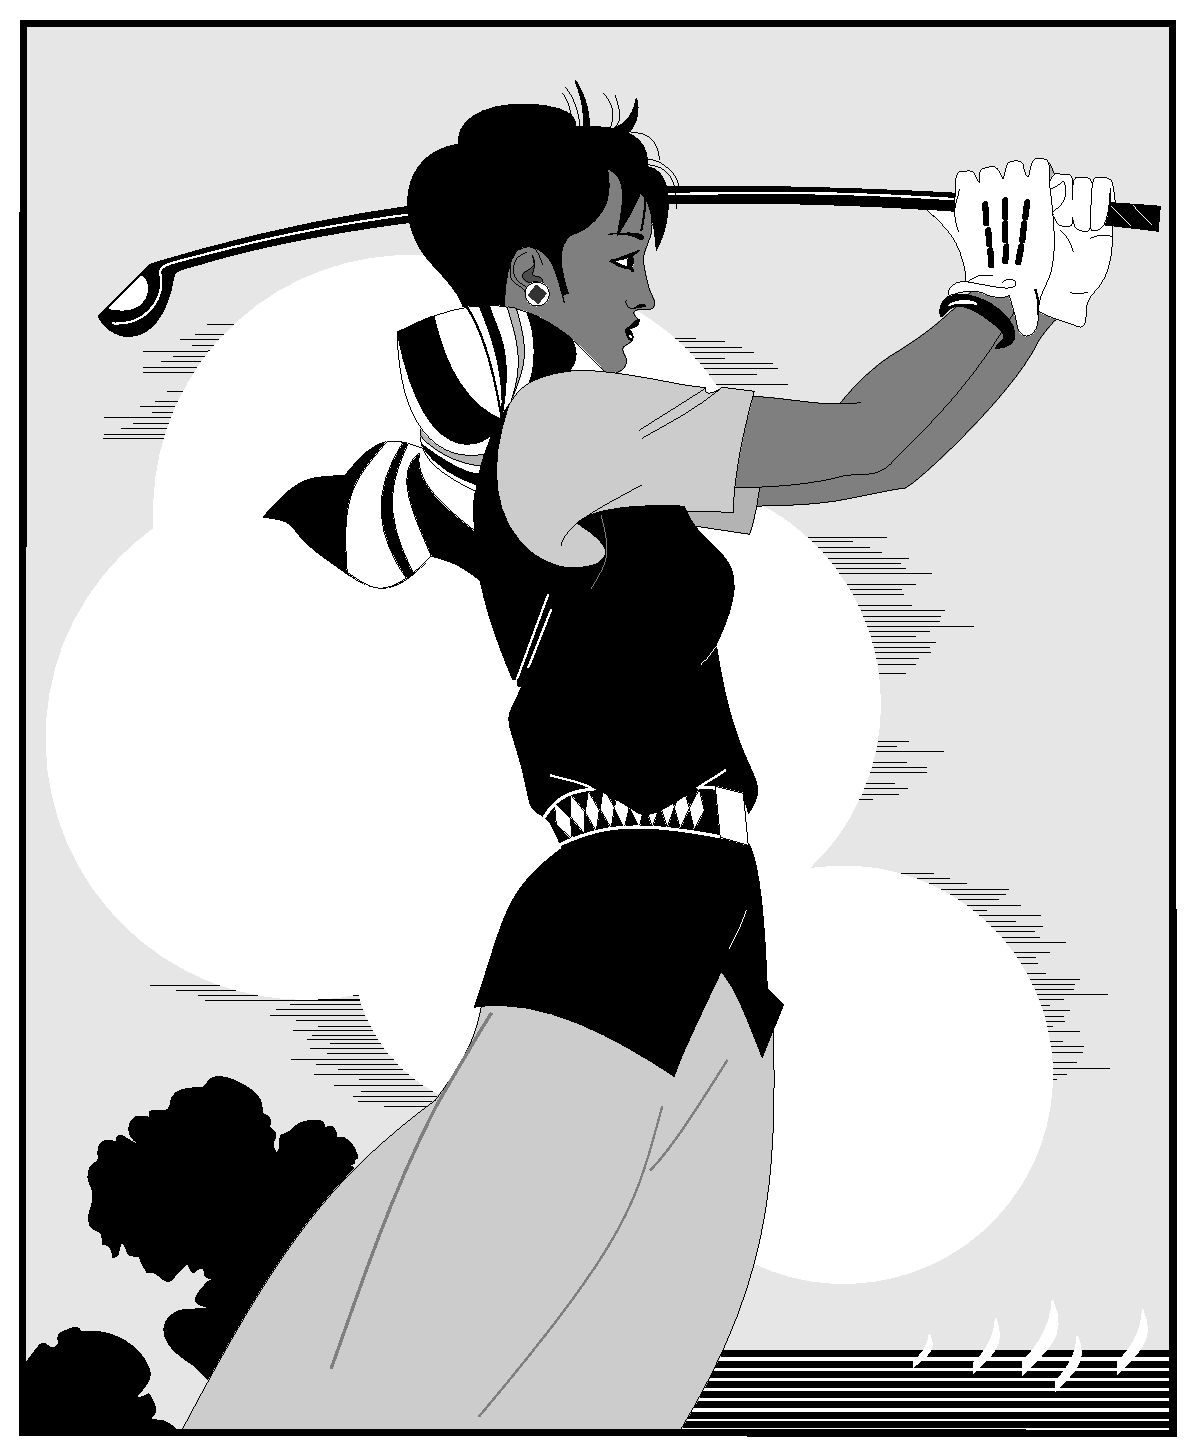
\includegraphics[width = 0.4\textwidth]{golfer}
% \bicaption[golfer1]{}{注意图中文字尽量用五号字
% }{Fig.$\!$}{The person playing golf}
% \end{figure}
% \end{latex}
% 单张单图题的格式如下,
% \begin{latex}
% \begin{figure}[h]
% \centering
% 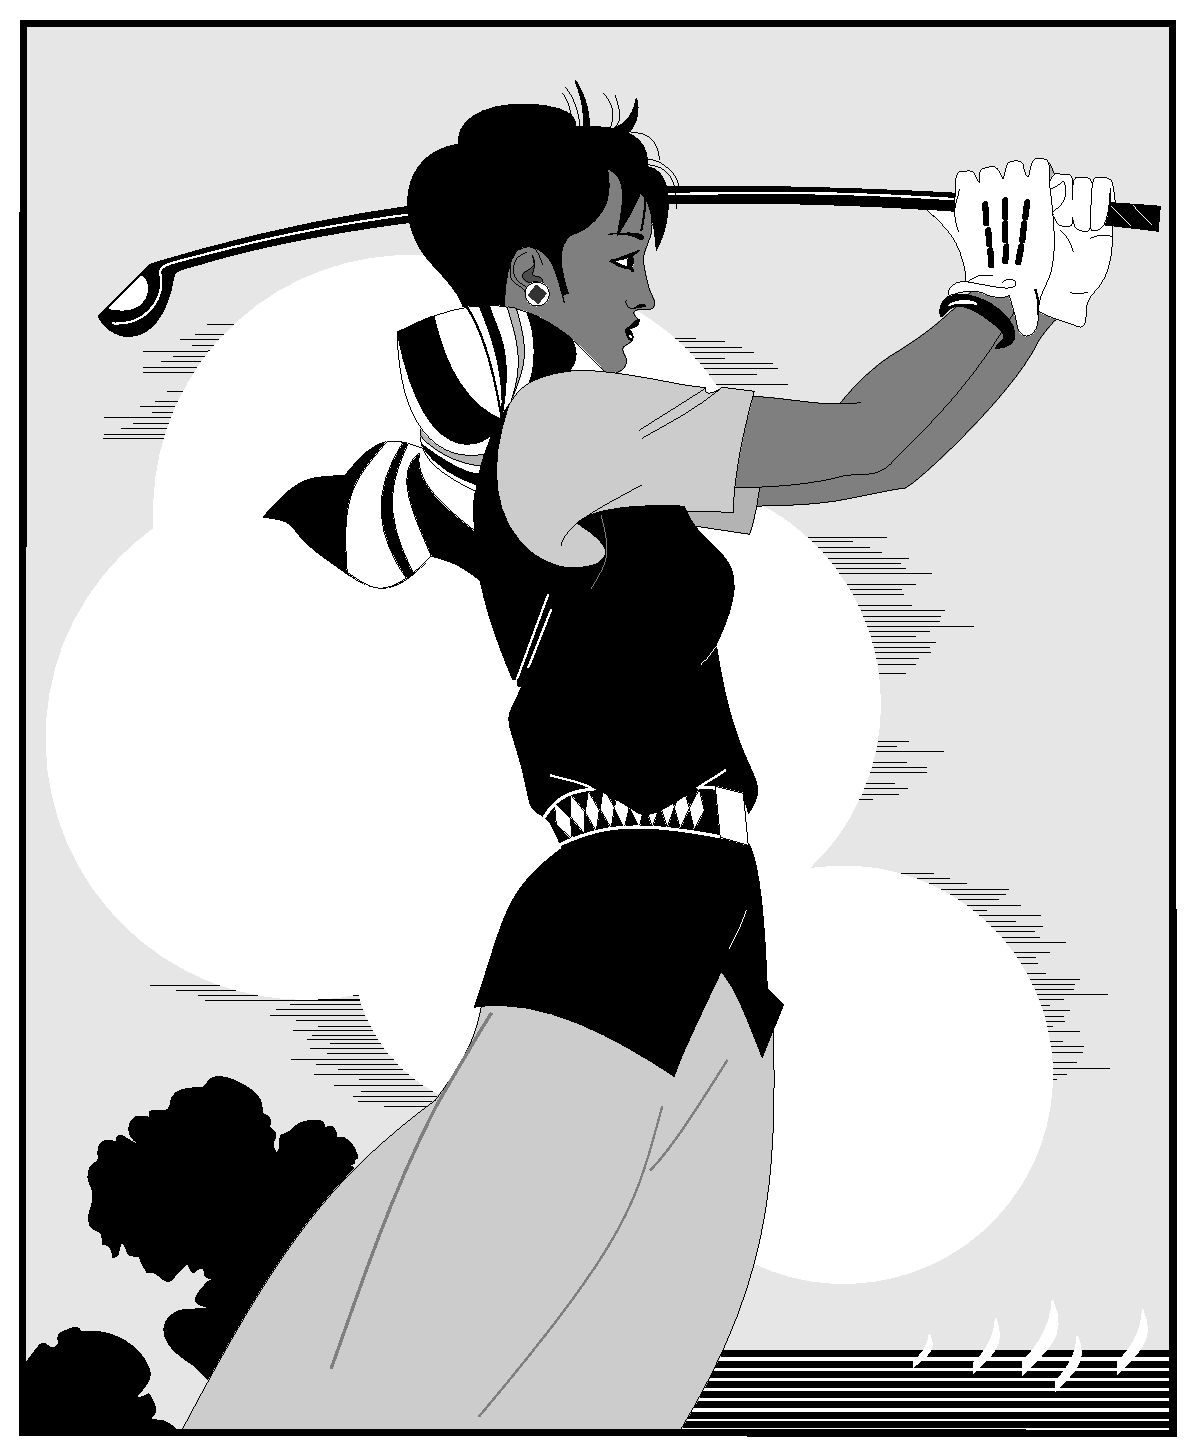
\includegraphics[width = 0.4\textwidth]{golfer}
% \caption{注意图中文字字号尽量用五号字}
% \end{figure}
% \end{latex}
% 并排图例。
% \begin{latex}
% \begin{figure}[htbp]
% \centering
% \begin{minipage}{0.4\textwidth}
% \centering
% 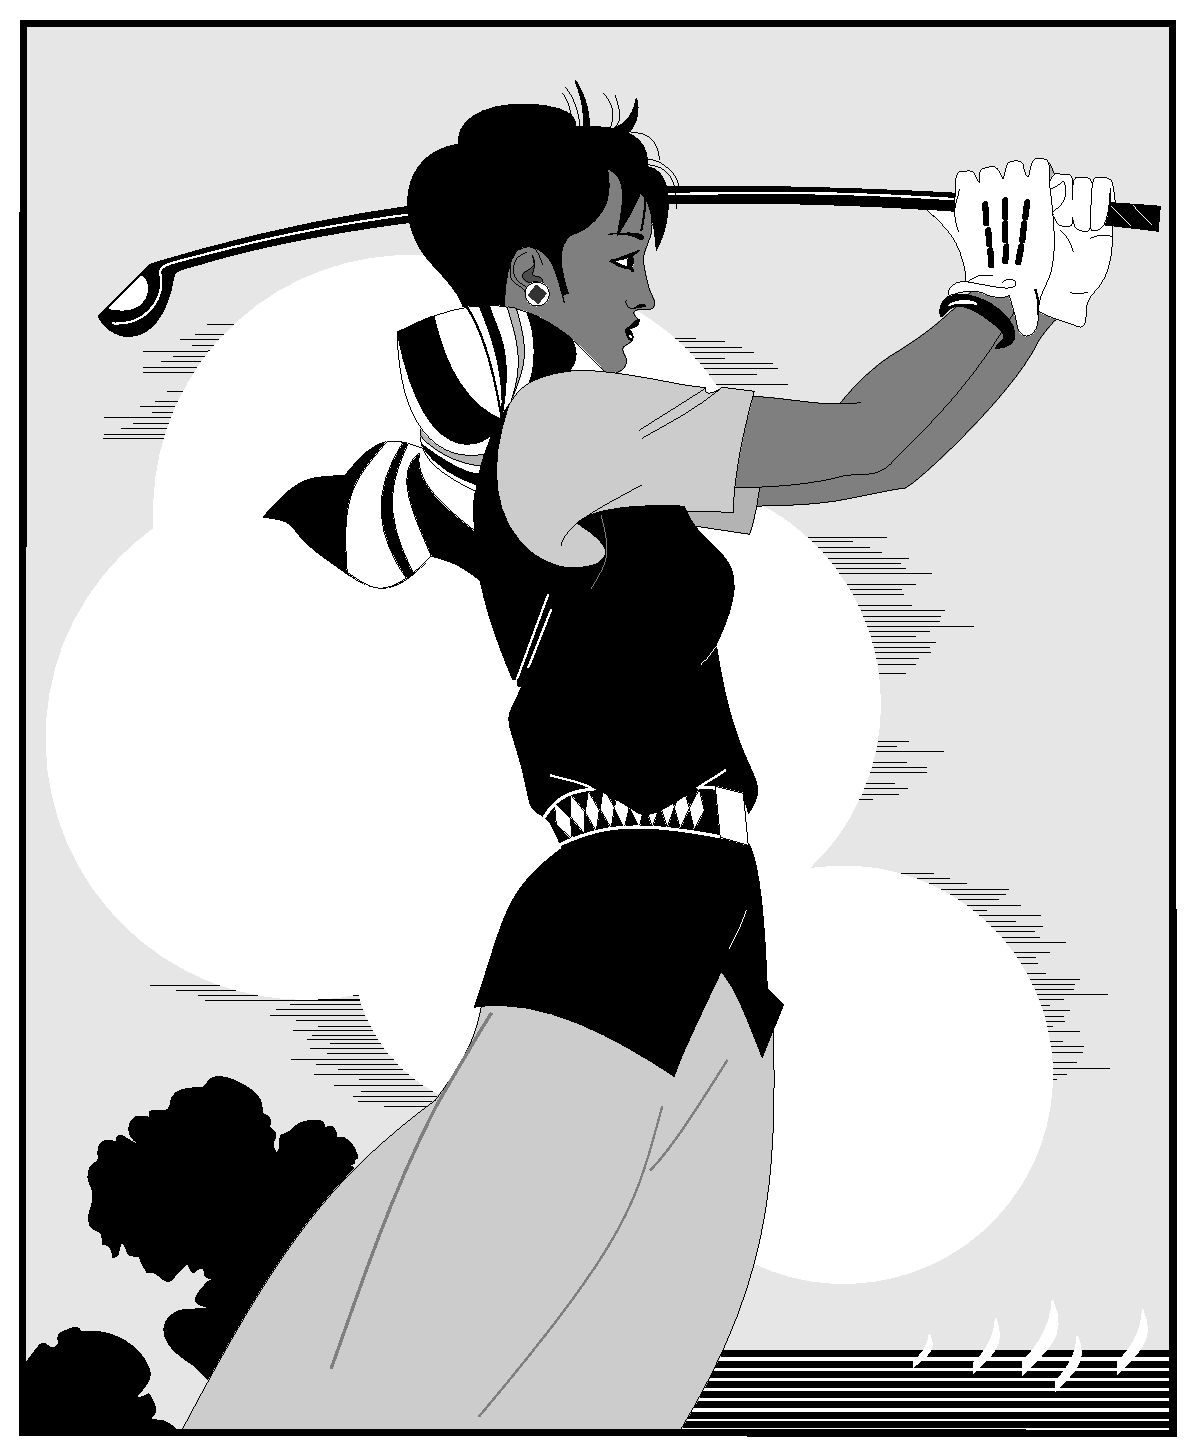
\includegraphics[width=\textwidth]{golfer}
% \bicaption[golfer2]{}{打高尔夫球的人}{Fig.$\!$}{The person playing golf}
% \end{minipage}
% \begin{minipage}{0.4\textwidth}
% \centering
% 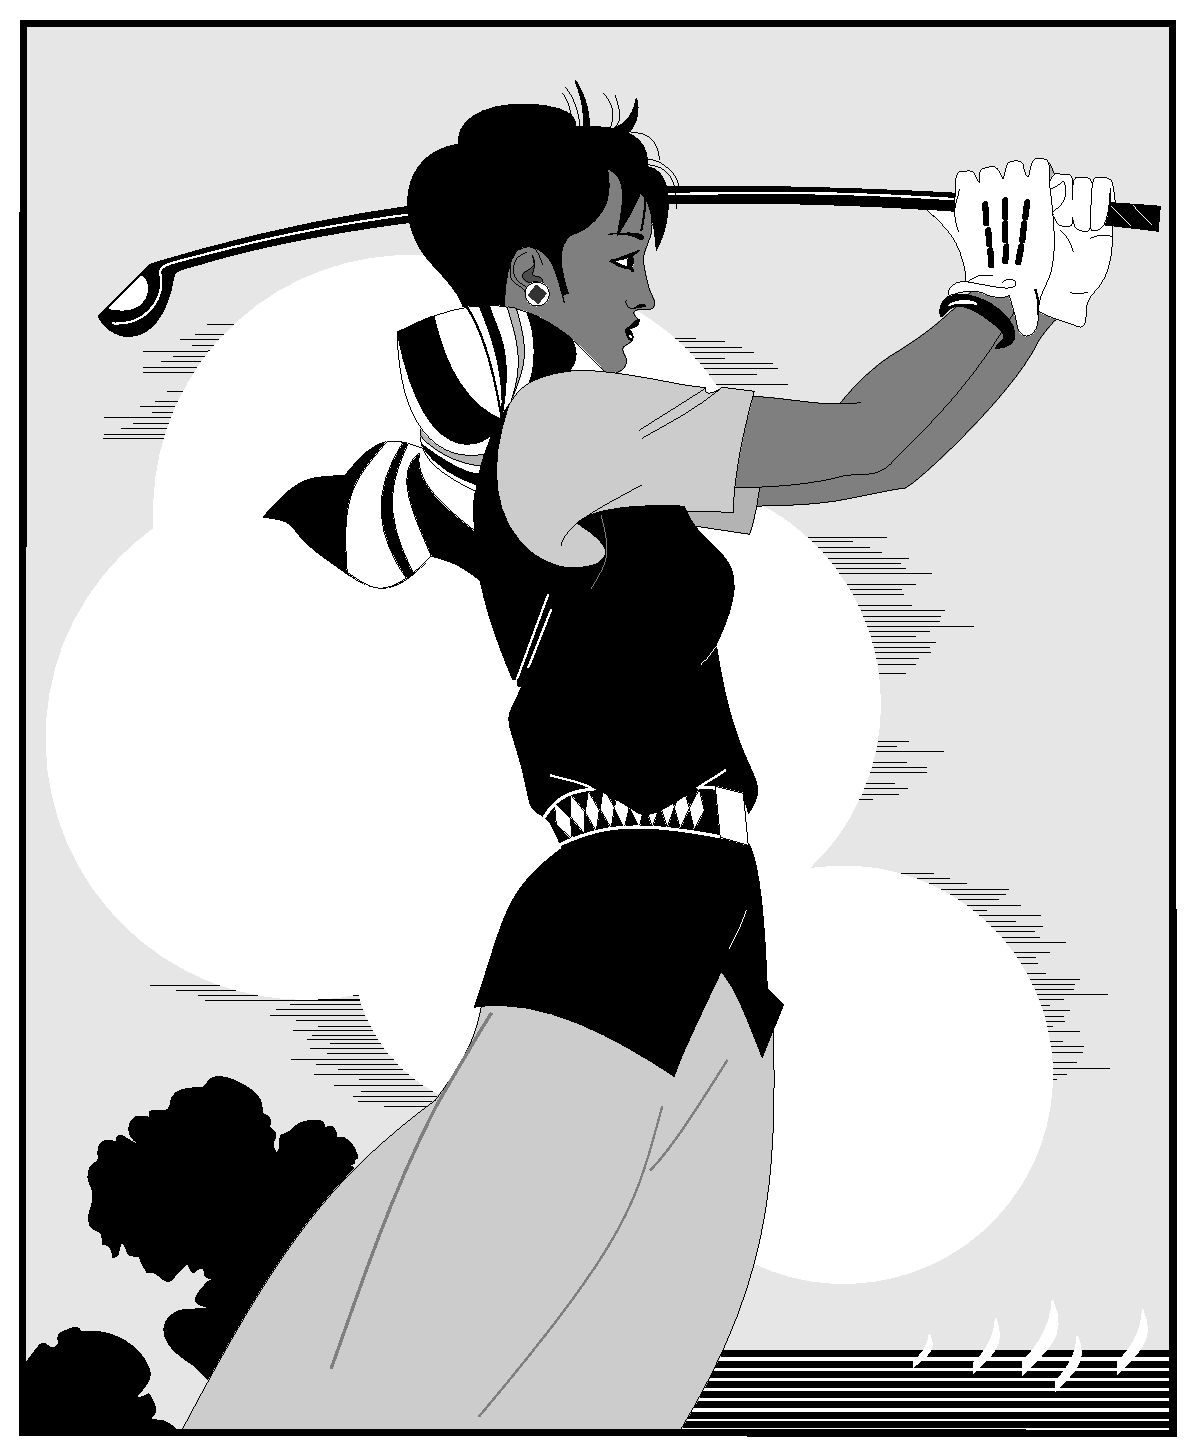
\includegraphics[width=\textwidth]{golfer}
% \bicaption[golfer3]{}{打高尔夫球的人}{Fig.$\!$}{The person playing golf}
% \end{minipage}
% \end{figure}
% \end{latex}
% 子图图例。
% \begin{latex}
% \begin{figure}[htbp]
% \centering
% \subfigure{\label{golfer41}}\addtocounter{subfigure}{-2}
% \subfigure[The person playing golf]{\subfigure[打高尔夫球的人~1]{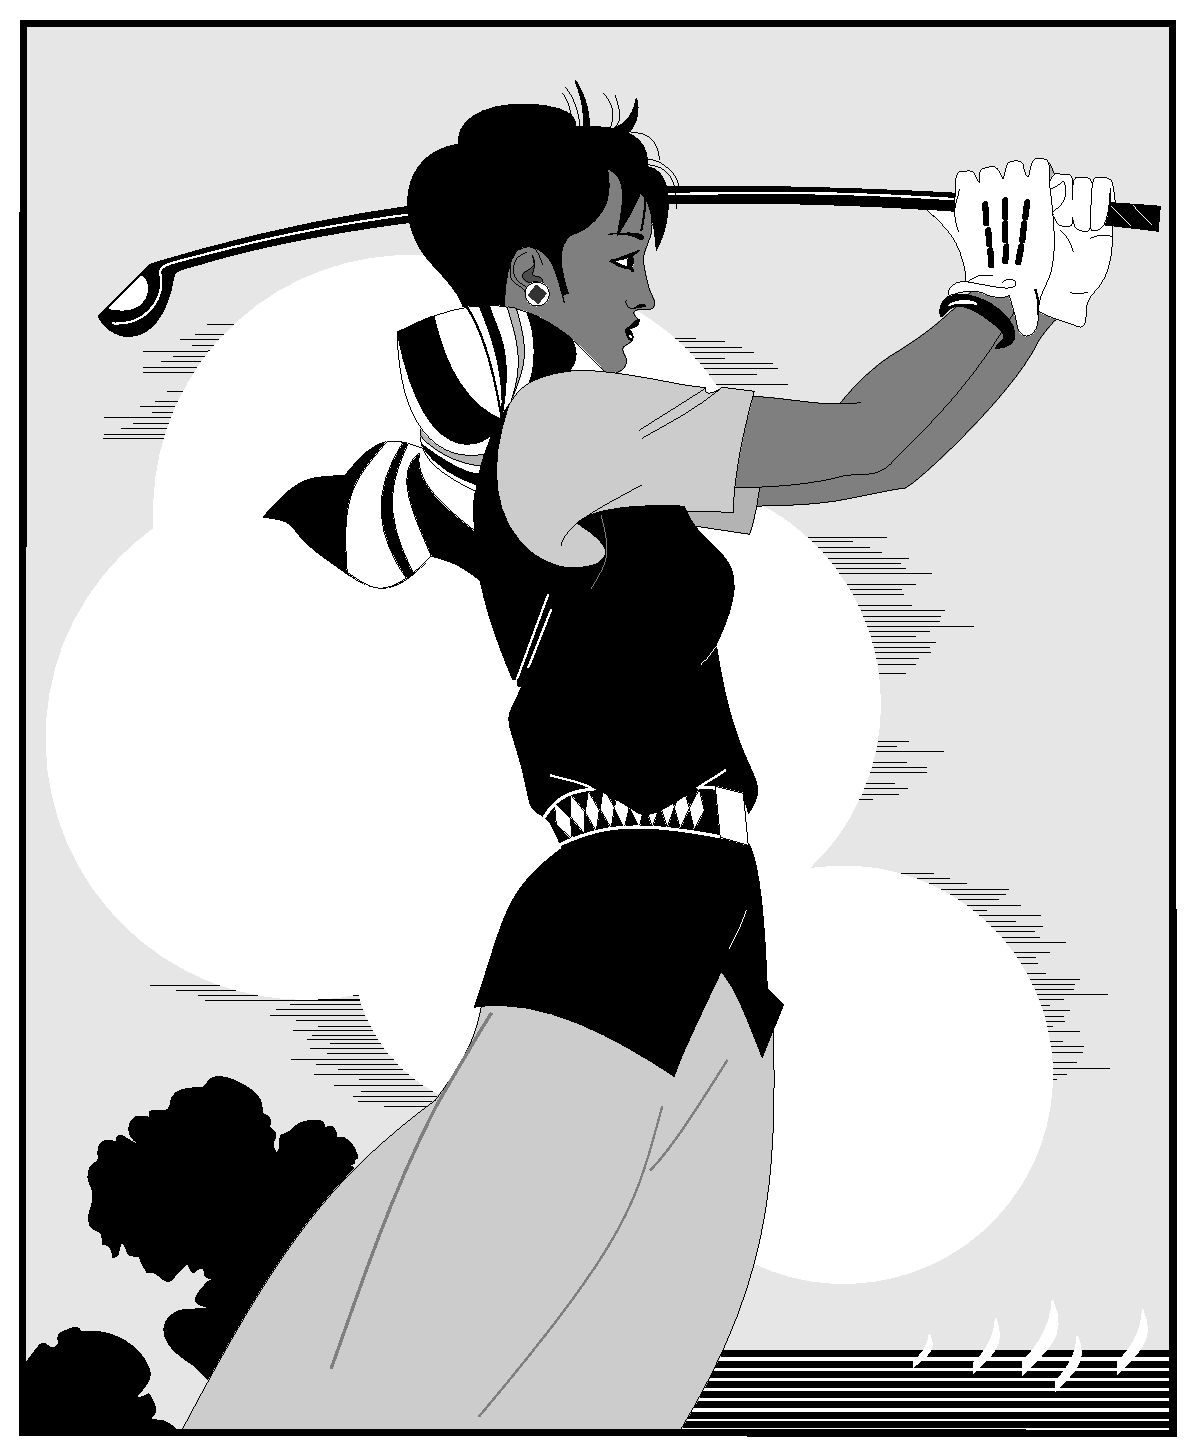
\includegraphics[width=0.4\textwidth]{golfer}}}
% \subfigure{\label{golfer42}}\addtocounter{subfigure}{-2}
% \subfigure[The person playing golf]{\subfigure[打高尔夫球的人~2]{\includegraphics[width=0.4\textwidth]{golfer}}}
% \bicaption[golfer4]{}{打高尔夫球的人}{Fig.$\!$}{The person playing golf}
% \end{figure}
% \end{latex}
% 表格示例,表格中的字体是可以自行调整的。
% \begin{latex}
% \begin{table}[htbp]
% \bicaption[table1]{}{符合研究生院绘图规范的表格}{Table$\!$}{Table in agreement of the standard from graduate school}
% \vspace{0.5em}\centering\wuhao
% \begin{tabular}{ccccc}
% \toprule[1.5pt]
% $D$(in) & $P_u$(lbs) & $u_u$(in) & $\beta$ & $G_f$(psi.in)\\
% \midrule[1pt]
%  5 & 269.8 & 0.000674 & 1.79 & 0.04089\\
% 10 & 421.0 & 0.001035 & 3.59 & 0.04089\\
% 20 & 640.2 & 0.001565 & 7.18 & 0.04089\\
% \bottomrule[1.5pt]
% \end{tabular}
% \end{table}
% \end{latex}
% 因为长表格不是浮动体,不会自动调整位置、也不会自动调整字体大小,一切都要手动设
% 置。特别繁琐。
% \begin{latex}
% \ltfontsize{\dawu[1.667]} %设置表格内字体行间距
% \dawu[1.667]\begin{longtable}{ccc} % 注意此处设置的是表格线距离
% \longbionenumcaption{}{{\wuhao 中国省级行政单位一览 %此处要添加字体设置
% }\label{table2}}{Table$\!$}{}{{\wuhao Overview of the provincial administrative
% unit of China}}{-0.5em}{3.15bp}\\ %注意后两个参数分别是中英标题间距、标题和表格的间距。
% %\caption{\wuhao 中国省级行政单位一览}\\[1em] %注意此处是标题和表格间距,这行
% %是单语标题
% \toprule[1.5pt] 名称 & 简称 & 省会或首府  \\ \midrule[1pt]
% \endfirsthead
% \multicolumn{3}{r}{表~\thetable(续表)}\vspace{0.5em}\\
% \toprule[1.5pt] 名称 & 简称 & 省会或首府  \\ \midrule[1pt]
% \endhead
% \bottomrule[1.5pt]
% \endfoot
% 北京市 & 京 & 北京\\
% 天津市 & 津 & 天津\\
% 河北省 & 冀 & 石家庄市\\
% 山西省 & 晋 & 太原市\\
% 内蒙古自治区 & 蒙 & 呼和浩特市\\
% 辽宁省 & 辽 & 沈阳市\\
% 吉林省 & 吉 & 长春市\\
% 黑龙江省 & 黑 & 哈尔滨市\\
% 上海市 & 沪/申 & 上海\\
% 江苏省 & 苏 & 南京市\\
% 浙江省 & 浙 & 杭州市\\
% 安徽省 & 皖 & 合肥市\\
% 福建省 & 闽 & 福州市\\
% 江西省 & 赣 & 南昌市\\
% 山东省 & 鲁 & 济南市\\
% 河南省 & 豫 & 郑州市\\
% 湖北省 & 鄂 & 武汉市\\
% 湖南省 & 湘 & 长沙市\\
% 广东省 & 粤 & 广州市\\
% 广西壮族自治区 & 桂 & 南宁市\\
% 海南省 & 琼 & 海口市\\
% 重庆市 & 渝 & 重庆\\
% 四川省 & 川/蜀 & 成都市\\
% 贵州省 & 黔/贵 & 贵阳市\\
% 云南省 & 云/滇 & 昆明市\\
% 西藏自治区 & 藏 & 拉萨市\\
% 陕西省 & 陕/秦 & 西安市\\
% 甘肃省 & 甘/陇 & 兰州市\\
% 青海省 & 青 & 西宁市\\
% 宁夏回族自治区 & 宁 & 银川市\\
% 新疆维吾尔自治区 & 新 & 乌鲁木齐市\\
% 香港特别行政区 & 港 & 香港\\
% 澳门特别行政区 & 澳 & 澳门\\
% 台湾省 & 台 & 台北市\\
% \end{longtable}\normalsize %注意这里要恢复正常字体
% \end{latex}
% \subsubsection{公式}
% 公式不做介绍,与正常用法一致。
% \subsubsection{数学环境}
% \label{sec:math}
% \hithesis\ 定义了常用的数学环境:
%
% \begin{center}
% \begin{tabular}{*{7}{l}}\toprule
%   axiom & theorem & definition & proposition & lemma & conjecture &\\
%   公理 & 定理 & 定义 & 命题 & 引理 & 猜想 &\\\midrule
%   proof & corollary & example & exercise & assumption & remark & problem \\
%   证明 & 推论 & 例子& 练习 & 假设 & 注释 & 问题\\\bottomrule
% \end{tabular}
% \end{center}
%
% 比如:
% \begin{latex}
% \begin{definition}
%   道千乘之国,敬事而信,节用而爱人,使民以时。
% \end{definition}
% \end{latex}
% 产生(自动编号):
% \medskip
%
% \noindent\framebox[\linewidth][l]{{\heiti 定义~1.1~~~} % {道千乘之国,敬事而信,节用而爱人,使民以时。}}
%
% \smallskip
% 列举出来的数学环境毕竟是有限的,如果想用\emph{胡说}这样的数学环境,那么可以定义:
% \begin{latex}
% \newtheorem{nonsense}{胡说}[chapter]
% \end{latex}
%
% 然后这样使用:
% \begin{latex}
% \begin{nonsense}
%   契丹武士要来中原夺武林秘笈。—— 慕容博
% \end{nonsense}
% \end{latex}
% 产生(自动编号):
%
% \medskip
% \noindent\framebox[\linewidth][l]{{\heiti 胡说~1.1~~~} % {契丹武士要来中原夺武林秘笈。—— 慕容博}}
% \subsubsection{算法}
% 我工算法不在规范中要求且一千个评审老师有一千个算法格式喜好。详见
% \href{https://github.com/PlutoThesis/PlutoThesis#%E6%B2%A1%E6%9C%89%E6%98%8E%E7%A1%AE%E8%A6%81%E6%B1%82%E7%9A%84%E6%A0%BC%E5%BC%8F}{PlutoThesis}
% 中的各个实验室算法喜好举例。在此多说无益。
% \subsubsection{引用参考文献}
% \DescribeMacro{\inlinecite}
% 学校要求的参考文献引用有两种模式:(1)上标模式。比如``同样的工作有很
% 多$^{[1,2]}$\ldots''。(2)正文模式。比如``文[3] 中详细说明了\ldots''。其中上标
% 模式使用远比正文模式频繁,所以为了符合使用习惯,上标模式仍然用常规
% 的 \cs{cite}\marg{key},而 \cs{inlinecite}\marg{key} 则用来生成正文模式。
%
% 关于参考文献模板推荐使用 \BibTeX,关于中文参考文献需要额外增加一个 Entry:
% \texttt{lang},将其设置为 \texttt{zh} 用来指示此参考文献为中文,以
% 便 \file{hithesis.bst} 处理。如:
% \begin{latex}
% @INPROCEEDINGS{cnproceed,
%   author    = {王重阳 and 黄药师 and 欧阳峰 and 洪七公 and 段皇帝},
%   title     = {武林高手从入门到精通},
%   booktitle = {第~$N$~次华山论剑},
%   year      = 2006,
%   address   = {西安, 中国},
%   month     = sep,
%   lang      = "zh",
% }
%
% @ARTICLE{cnarticle,
%   AUTHOR  = "贾宝玉 and 林黛玉 and 薛宝钗 and 贾探春",
%   TITLE   = "论刘姥姥食量大如牛之现实意义",
%   JOURNAL = "红楼梦杂谈",
%   PAGES   = "260--266",
%   VOLUME  = "224",
%   YEAR    = "1800",
%   LANG    = "zh",
% }
% \end{latex}
%
% 注意如果不需要引用参考文献,请删除 \file{main.tex} 中 \cs{bibliography} 开头的两行,
% 以避免可能的编译错误。
%
% \subsubsection{列表环境}
% \DescribeEnv{itemize}
% \DescribeEnv{enumerate}
% \DescribeEnv{description}
% 为了适合中文习惯,模板将这三个常用的列表环境用 \pkg{enumitem} 进行了纵向间距压
% 缩。一方面清除了多余空间,另一方面用户可以自己指定列表环境的样式(如标签符号,
% 缩进等)。细节请参看 \pkg{enumitem} 文档,此处不再赘述。
% \subsection{后文}
%
% \subsubsection{结论}
% \DescribeEnv{conclusion}
% 结论之后为后文内容。
% \begin{latex}
% \begin{conclusions}
%
% 学位论文的结论作为论文正文的最后一章单独排写,但不加章标题序号。
%
% 结论应是作者在学位论文研究过程中所取得的创新性成果的概要总结,不能与摘要混为一
% 谈。博士学位论文结论应包括论文的主要结果、创新点、展望三部分,在结论中应概括论
% 文的核心观点,明确、客观地指出本研究内容的创新性成果(含新见解、新观点、方法创
% 新、技术创新、理论创新),并指出今后进一步在本研究方向进行研究工作的展望与设想
% 。对所取得的创新性成果应注意从定性和定量两方面给出科学、准确的评价,分(1)、
% (2)、(3)…条列出,宜用“提出了”、“建立了”等词叙述。
%
% \end{conclusions}
% \end{latex}
%
% \subsubsection{参考文献}
% 在后文中的参考文献是自动生成的,不需要用户干预,具体命令在\file{main.tex}中有
% 示例。
%
% \subsubsection{附录}
% \DescribeEnv{appendix}
% 所有的附录都插到这里来。因为附录会更改默认的 chapter 属性,而后面的{\heiti 个人简
%   历}又需要恢复,所以实现为环境可以保证全局的属性不受影响。
% \begin{latex}
% \begin{appendix}
% \input{back/appA.tex}
% \end{appendix}
% \end{latex}
%
% \subsubsection{所发表文章}
% \DescribeEnv{publication}
% 虽然在\PGR\UGR\ 中都没有明确规定此处的格式,但按照旧模板PlutoThesis,此处格式
% 非常复杂。此处仍然使用旧模板中的设置方法。
% \begin{latex}
% \begin{publication}
% \noindent\textbf{(一)发表的学术论文}
% \begin{publist}
% \item	XXX,XXX. Static Oxidation Model of Al-Mg/C Dissipation Thermal Protection Materials[J]. Rare Metal Materials and Engineering, 2010, 39(Suppl. 1): 520-524.(SCI~收录,IDS号为~669JS,IF=0.16)
% \item XXX,XXX. 精密超声振动切削单晶铜的计算机仿真研究[J]. 系统仿真学报,2007,19(4):738-741,753.(EI~收录号:20071310514841)
% \item XXX,XXX. 局部多孔质气体静压轴向轴承静态特性的数值求解[J]. 摩擦学学报,2007(1):68-72.(EI~收录号:20071510544816)
% \item XXX,XXX. 硬脆光学晶体材料超精密切削理论研究综述[J]. 机械工程学报,2003,39(8):15-22.(EI~收录号:2004088028875)
% \item XXX,XXX. 基于遗传算法的超精密切削加工表面粗糙度预测模型的参数辨识以及切削参数优化[J]. 机械工程学报,2005,41(11):158-162.(EI~收录号:2006039650087)
% \item XXX,XXX. Discrete Sliding Mode Cintrok with Fuzzy Adaptive Reaching Law on 6-PEES Parallel Robot[C]. Intelligent System Design and Applications, Jinan, 2006: 649-652.(EI~收录号:20073210746529)
% \end{publist}
%
% \noindent\textbf{(二)申请及已获得的专利(无专利时此项不必列出)}
% \begin{publist}
% \item XXX,XXX. 一种温热外敷药制备方案:中国,88105607.3[P]. 1989-07-26.
% \end{publist}
%
% \noindent\textbf{(三)参与的科研项目及获奖情况}
% \begin{publist}
% \item	XXX,XXX. XX~气体静压轴承技术研究, XX~省自然科学基金项目.课题编号:XXXX.
% \item XXX,XXX. XX~静载下预应力混凝土房屋结构设计统一理论. 黑江省科学技术二等奖, 2007.
% \end{publist}
% %\vfill
% %\hangafter=1\hangindent=2em\noindent
% %\setlength{\parindent}{2em}
% \end{publication}
% \end{latex}
%
% \subsubsection{索引}
% \DescribeEnv{ceindex}
% 我工要求中英文双语索引。后文中的自动索引实际上不需要用户干预。
%\begin{latex}
% \begin{ceindex}
%   %如果想要手动加索引,注释掉以下这一样,用wordlist环境
% \printsubindex*
% \end{ceindex}
%\end{latex}
% 手工添加索引的方法不推荐,模板中将去除该功能。
% \subsubsection{授权}
% \DescribeMacro{\authorization}
% 授权页中的签名和日期是需要手写,不需要人工干预。具体示例在\file{main.tex}中。
%\begin{latex}
% \authorization %授权
% %\authorization[saomiao.pdf] %添加扫描页的命令,与上互斥
%\end{latex}
%
% \subsubsection{致谢声明}
% \DescribeEnv{acknowledgement}
% 把致谢做成一个环境更好一些,直接往里面写感谢的话就可以啦!
%
% \begin{latex}
% \begin{acknowledgement}
%   …
%   感谢\hit\LaTeX\ 论文模板\hithesis\ !
% \end{acknowledgement}
% \end{latex}
%
%
% \subsubsection{简历}
% \DescribeEnv{resume}
% 个人简历。
% 实际上,致谢和个人简历是自由发挥的地区,字体,文体,格式,内容,完全自己决定。
% \begin{latex}
% \begin{resume}
% XXXX~年~XX~月~XX~日出生于~XXXX。
%
% XXXX~年~XX~月考入~XX~大学~XX~院(系)XX~专业,XXXX~年~XX~月本科毕业并获得~XX~学学士学位。
%
% XXXX~年~XX~月------XXXX~年~XX~月在~XX~大学~XX~院(系)XX~学科学习并获得~XX~学硕士学位。
%
% XXXX~年~XX~月------XXXX~年~XX~月在~XX~大学~XX~院(系)XX~学科学习并获得~XX~学博士学位。
%
% 获奖情况:如获三好学生、优秀团干部、X~奖学金等(不含科研学术获奖)。
%
% 工作经历:
% \end{resume}
% \end{latex}
%
% \subsection{其它}
% 模板的配置文件 \file{hithesis.cfg} 中定义了很多固定词汇,一般无须修改。如果有特殊需求,
% 推荐在导言区使用 \cs{renewcommand}。
%
%
% \subsection{捐助}
% \changes{v1.0.1}{2017/08/27}{添加了捐助、矢量化本科论文模板的图片logo}
% 各位刀客和大侠如用的嗨,要解囊相助,请微信或支付宝参照图
% ~\ref{wct5}-\ref{zfb}~中提示操作(二维码被矢量化后之后去
% 除了头像等冗余无用的部分~)。
% \begin{figure}[h]
% \centering\includegraphics[width=0.5\textwidth]{wct5.eps}
% \caption{如果用的嗨,微信扫码捐助5元~~}
% \label{wct5}
% \end{figure}
% \begin{figure}[h]
% \centering\includegraphics[width=0.5\textwidth]{wct10.eps}
% \caption{如果用的非常嗨,微信扫码捐助10元~~}
% \label{wct10}
% \end{figure}
% \begin{figure}[h]
% \centering\includegraphics[width=0.5\textwidth]{wct1.eps}
% \caption{那个,看在熬夜写代码的份上,微信扫码捐助1元吧~~}
% \label{wct1}
% \end{figure}
% \begin{figure}[h]
% \centering\includegraphics[width=0.5\textwidth]{zfb.eps}
% \caption{支付宝不限额度}
% \label{zfb}
% \end{figure}
%
% \StopEventually{\PrintChanges\PrintIndex}
% \clearpage
%
% \section{实现细节}
%
% \subsection{基本信息}
%    \begin{macrocode}
%<cls>\NeedsTeXFormat{LaTeX2e}[1999/12/01]
%<cls>\ProvidesClass{hithesis}
%<cfg>\ProvidesFile{hithesis.cfg}
%<cls|cfg>[2018/12/05 2.0.6 Harbin Institute of Technology Thesis Template]
%    \end{macrocode}
%
% \subsection{定义选项}
% \label{sec:defoption}
%    \begin{macrocode}
%<*cls>
\RequirePackage{ifthen}
\RequirePackage{kvoptions}
\SetupKeyvalOptions{
  family=hit,
  prefix=hit@,
  setkeys=\kvsetkeys}
\newif\ifhit@bachelor
\newif\ifhit@master
\newif\ifhit@doctor
\define@key{hit}{type}{%
  \hit@bachelorfalse
  \hit@masterfalse
  \hit@doctorfalse
  \expandafter\csname hit@#1true\endcsname}
%    \end{macrocode}
%	定义stage项,区分开题、中期,默认false,为毕业论文,empty为空-去掉页眉 _added by t
%    \begin{macrocode}
\newif\ifhit@kaiti
\newif\ifhit@zhongqi
\define@key{hit}{stage}{%
  \hit@kaitifalse
  \hit@zhongqifalse
  \expandafter\csname hit@#1true\endcsname}
%    \end{macrocode}
%    设置版芯,由于窝工版芯歧义。
% \changes{v2.0.0}{2018/6/14}{此处添加geometry选项}
%    \begin{macrocode}
\newif\ifhit@geometrynewone
\newif\ifhit@geometrynewtwo
\define@key{hit}{newgeometry}{%
  \hit@geometrynewonefalse
  \hit@geometrynewtwofalse
  \expandafter\csname hit@geometrynew#1true\endcsname}
%    \end{macrocode}
% 目录中英文是否用 Arial 字体(默认关闭)。
%    \begin{macrocode}
\DeclareBoolOption[false]{arialtoc}
%    \end{macrocode}
% 章节标题中的英文是否用 Arial 字体(默认打开)。
%    \begin{macrocode}
\DeclareBoolOption[false]{arialtitle}
%    \end{macrocode}
% \changes{v1.0.3}{2017/08/29}{默认开启raggedbottom}
% \option{raggedbottom} 选项(默认开启)。如果不开启这个选项,会出现一页中尽量上
% 下对齐,段的间距大。如果开启,尽量使段间距保持一致,页面底部出现空白。
%    \begin{macrocode}
\DeclareBoolOption[true]{raggedbottom}
%    \end{macrocode}
% 在脚注标记中使用 \pkg{pifont} 的带圈数字(默认关闭)。
%    \begin{macrocode}
\DeclareBoolOption[false]{pifootnote}
%    \end{macrocode}
% 字体间距设置(默认关闭)。
%    \begin{macrocode}
\DeclareBoolOption[false]{glue}
%    \end{macrocode}
% 文科生四级目录设置(默认关闭)。
%    \begin{macrocode}
\DeclareBoolOption[false]{tocfour}
%    \end{macrocode}
% 目录中“目录”位置是否空行(默认开启)。
%    \begin{macrocode}
\DeclareBoolOption[true]{tocblank}
%    \end{macrocode}
% 章标题是否悬挂居中(默认开启)
%    \begin{macrocode}
\DeclareBoolOption[true]{chapterhang}
%    \end{macrocode}
% 是否是全日制学生(默认是)。
%    \begin{macrocode}
\DeclareBoolOption[true]{fulltime}
%    \end{macrocode}
% 是否有子标题(默认是)。
%    \begin{macrocode}
\DeclareBoolOption[false]{subtitle}
%    \end{macrocode}
% 是否开启debug模式(默认否)。如果开启,载入显示行号等的包,只为开发调试用。
%    \begin{macrocode}
\DeclareBoolOption[false]{debug}
%    \end{macrocode}
% \changes{v2.0.0}{2018/6/14}{此处删除newgeometry选项}
% 是否使用右开页(默认否)。
%    \begin{macrocode}
\DeclareBoolOption[false]{openright}
%    \end{macrocode}
% 图题和标题最后一行是否居中对其(默认是,非规范要求)。
% \changes{v1.0.6}{2017/10/25}{此处更改了选项的名称}
%    \begin{macrocode}
\DeclareBoolOption[false]{capcenterlast}
%    \end{macrocode}
% 子图图题和标题最后一行是否居中对其(默认是,非规范要求)。
% \changes{v1.0.6}{2017/10/25}{此处添加子图最后一行图题是否居中选项}
%    \begin{macrocode}
\DeclareBoolOption[false]{subcapcenterlast}
%    \end{macrocode}
% 中文目录中Abstract是否均为大写
% \changes{v1.0.13}{2018/4/5}{此处添加中文目录中Abstract是否均为大写选项}
%    \begin{macrocode}
\DeclareBoolOption[false]{absupper}
%    \end{macrocode}
%    此处添加控制本科论文的页码横线选项
% \changes{v1.0.15}{2018/06/05}{添加控制本科论文的页码横线选项}
%    \begin{macrocode}
\DeclareBoolOption[false]{bsmainpagenumberline}
\DeclareBoolOption[false]{bsfrontpagenumberline}
\DeclareBoolOption[true]{bsheadrule}
%    \end{macrocode}
%    数学字体是否使用新罗马
% \changes{v2.0.5}{2018/12/05}{添加数学字体开关}
%    \begin{macrocode}
\DeclareBoolOption[true]{newtxmath}
%    \end{macrocode}
%    此处应广大刀客要求添加一参考文献分割开关
% \changes{v2.0.3}{2018/10/08}{添加参考文献分割开关}
%    \begin{macrocode}
\DeclareBoolOption[false]{splitbibitem}
%    \end{macrocode}
% 声明字体选项。
%    \begin{macrocode}
\DeclareBoolOption[false]{customheadfancy}
%	添加customheadfancy项,可以用来自定义页眉,默认false,暂时无用  _added by t
\DeclareBoolOption[false]{noheader}
%	添加noheader项,true时可以用来去掉页眉(开题、中期报告老师可能不让留页眉),默认false,保留页眉  _added by t
\DeclareStringOption{fontset}
%    \end{macrocode}
% 将其余选项默认传递给 \pkg{ctexbook}。
%    \begin{macrocode}
\DeclareDefaultOption{\PassOptionsToClass{\CurrentOption}{ctexbook}}
%    \end{macrocode}
% 解析用户传递过来的选项,并加载 \pkg{ctexbook}。
%    \begin{macrocode}
\ProcessKeyvalOptions*
%    \end{macrocode}
% 使用 \XeTeX\ 引擎时,\pkg{fontspec} 宏包会被 \pkg{xeCJK} 自动调用。传递
% 给 \pkg{fontspec} 宏包 \option{no-math} 选项,避免部分数学符号字体自动调整
% 为 CMR。其他引擎下没有这个问题,这一行会被无视。
%    \begin{macrocode}
\PassOptionsToPackage{no-math}{fontspec}
%    \end{macrocode}
% 载入单双面打印设置,本、硕单面,博士双面。
%    \begin{macrocode}
\ifhit@bachelor
\PassOptionsToClass{oneside}{book}
\fi
\ifhit@master
\PassOptionsToClass{oneside}{book}
\fi
\ifhit@doctor
\PassOptionsToClass{twoside}{book}
\fi
%    \end{macrocode}
% \changes{v1.0.2}{2017/08/27}{添加了思源字体说明}
% 设置字体。由于宋体没有粗体,且我工模板的标题要求使用粗宋体,于是面临CTeX的经典
% 的伪粗体bug:“首次出现伪粗体字体之后的正常字体无法复制”。但如果使用自带宋体的
% 思源字体,那么不必使用伪粗体。模板只给出了新windows字体的思源字体设置,且思源
% 字体版本为Adobe版。
%    \begin{macrocode}
\ifthenelse%
{\equal{\hit@fontset}{}}%
{%
  \PassOptionsToPackage{AutoFakeBold=2}{xeCJK}
}%
{%
  \ifthenelse%
  {\equal{\hit@fontset}{siyuan}}%
  {\relax}%
  {%
    \PassOptionsToPackage{AutoFakeBold=2}{xeCJK}
  }%
  \PassOptionsToClass{fontset=\hit@fontset}{ctexbook}
}%
%    \end{macrocode}
% 使用 \pkg{ctexbook} 类,优于调用 \pkg{ctex} 宏包。
%    \begin{macrocode}
\LoadClass[a4paper,openany,UTF8,zihao=-4,scheme=plain]{ctexbook}
%    \end{macrocode}
% 用户至少要提供一个选项,指定论文类型。
%    \begin{macrocode}
\ifhit@bachelor\relax\else
  \ifhit@master\relax\else
    \ifhit@doctor\relax\else
        \ClassError{hithesis}%
                   {Please specify thesis type in option: \MessageBreak
                    type=[bachelor | master | doctor]}{}
      \fi
  \fi
\fi
%    \end{macrocode}
%
% \subsection{装载宏包}
% \label{sec:loadpackage}
%
% 引用的宏包和相应的定义。
%    \begin{macrocode}
\RequirePackage{etoolbox}
\RequirePackage{ifxetex}
\ifxetex
\else
        \ClassError{hithesis}%
                   {Please use: \MessageBreak
                    xelatex}{}
\fi
\RequirePackage{xparse}
%    \end{macrocode}
%
% \AmSTeX\ 宏包,用来排出更加漂亮的公式。
%    \begin{macrocode}
\RequirePackage{amsmath}
%    \end{macrocode}
% \pkg{newtx} 设置 Times New Roman,Helvetica。
%    \begin{macrocode}
\RequirePackage[defaultsups]{newtxtext}
%    \end{macrocode}
% 添加数学字体开关
%    \begin{macrocode}
\ifhit@newtxmath
\RequirePackage{newtxmath}
\fi
%    \end{macrocode}
% \pkg{newtx} 的 Mono 字体虽然很好看,但在论文中不常见。学校虽未要求 Mono 字体,
% 还是选择常见的 Courier 字体。由于比较新的实现 \TeX\ Gyre Cursor 会修
% 改\cs{bfdefault},导致中文加粗出问题,所以选用标准 \pkg{courier}。
%    \begin{macrocode}
\RequirePackage{courier}
%    \end{macrocode}
% 图形支持宏包。
%    \begin{macrocode}
\RequirePackage{graphicx}
%    \end{macrocode}
% \pkg{pdfpages} 宏包便于我们插入扫描后的授权页和声明页 PDF 文档。
%    \begin{macrocode}
\RequirePackage{pdfpages}
\includepdfset{fitpaper=true}
%    \end{macrocode}
% 更好的列表环境。
%    \begin{macrocode}
\RequirePackage{enumitem}       %使用enumitem宏包,改变列表项的格式
\RequirePackage{environ}
%    \end{macrocode}
% 禁止 \LaTeX 自动调整多余的页面底部空白,并保持脚注仍然在底部。
% 脚注按页编号。
%    \begin{macrocode}
\ifhit@raggedbottom
  \RequirePackage[bottom,perpage,hang]{footmisc}
  \raggedbottom
\else
  \RequirePackage[perpage,hang]{footmisc}
\fi
%    \end{macrocode}
% 脚注格式。
%    \begin{macrocode}
\ifhit@pifootnote
  \RequirePackage{pifont}
\fi
%    \end{macrocode}
% 利用 \pkg{CJKfntef} 实现汉字的下划线和盒子内两段对齐,并可以避免
% \cs{makebox}\oarg{width}\oarg{s} 可能产生的 underful boxes。
%    \begin{macrocode}
\RequirePackage{CJKfntef}
%    \end{macrocode}
% 定理类环境宏包,其中 \pkg{amsmath} 选项用来兼容 \AmSTeX\ 的宏包
%    \begin{macrocode}
\RequirePackage[amsmath,thmmarks,hyperref]{ntheorem}
%    \end{macrocode}
% 表格控制
%    \begin{macrocode}
\RequirePackage{longtable}
%    \end{macrocode}
% 使用三线表:\cs{toprule},\cs{midrule},\cs{bottomrule}。
%    \begin{macrocode}
\RequirePackage{booktabs}
%    \end{macrocode}
% 参考文献引用宏包。
%    \begin{macrocode}
\RequirePackage[sort&compress]{natbib}
%    \end{macrocode}
% 生成有书签的 pdf 及其开关,请结合 gbk2uni 避免书签乱码。
%    \begin{macrocode}
\RequirePackage{hyperref}
\hypersetup{%
  CJKbookmarks=true,
  linktoc=all,
  bookmarksnumbered=true,
  bookmarksopen=true,
  bookmarksopenlevel=1,
  breaklinks=true,
  colorlinks=false,
  plainpages=false,
  pdfborder=0 0 0}
%    \end{macrocode}
% 设置 url 样式,与上下文一致
%    \begin{macrocode}
\urlstyle{same}
%    \end{macrocode}
%
% \subsection{页面设置}
% \label{sec:layout}
% 本来这部分应该是最容易设置的,但根据我工\PGR\ 的3.8,3.4,3.2节的版芯矛盾,此处
% 设置两种版芯。
%    \begin{macrocode}
\ifhit@debug\RequirePackage[showframe]{geometry}\else\RequirePackage{geometry}\fi
\geometry{%根据PlutoThesis 原版定义而来
  a4paper, % 210 * 297mm
  hcentering,
  ignoreall,
  nomarginpar,
}
%    \end{macrocode}
%    添加版芯设置选项
%    \changes{v2.0.0}{2018/6/14}{添加版芯设置选项}
%    \begin{macrocode}
\ifhit@geometrynewtwo%
	\geometry{
	  centering,
	  text={150true mm,236true mm},
	  left=30true mm,
	  head=5true mm,
	  headsep=2true mm,
	  footskip=0true mm,
	  foot=5.2true mm
	}
\else%
	\ifhit@geometrynewone%
		\geometry{
		  centering,
		  text={150true mm,240true mm},
		  left=30true mm,
		  head=5true mm,
		  headsep=0true mm,
		  footskip=0true mm,
		  foot=0true mm
		}
	\else%
		\geometry{%根据PlutoThesis 原版定义而来
			text={150true mm,224true mm},
			top=35.5true mm,
			left=30true mm,
			head=5true mm,
			headsep=2.5true mm,
			foot=8.5true mm
		}
	\fi%
\fi%
%    \end{macrocode}
%    载入显示行号的包。
% \changes{v1.0.9}{2018/01/07}{添加debug包}
%    \begin{macrocode}
\ifhit@debug%
\RequirePackage{layout}
\RequirePackage{layouts}
\RequirePackage{lineno}
\fi
%    \end{macrocode}
% 利用 \pkg{fancyhdr} 设置页眉页脚。
%    \begin{macrocode}
\RequirePackage{fancyhdr}
%    \end{macrocode}
% 其他包,表格、数学符号包
% \changes{v1.0.6}{2017/10/25}{此处添加子图最后一行图题是否居中选项}
%    \begin{macrocode}
\RequirePackage{tabularx}
\RequirePackage{varwidth}
%    \end{macrocode}
% 此处changepage环境用来控制索引页面的左右边距,规范中给出的示例的边距要大于正文。
% \changes{v1.0.10}{2018/02/19}{修改了索引的间距,使其更符合规范中的示例}
%    \begin{macrocode}
\RequirePackage{changepage}
\RequirePackage{multicol}
\RequirePackage{amssymb}
\RequirePackage[below]{placeins}%允许上一个section的浮动图形出现在下一个section的开始部分,还提供\FloatBarrier命令,使所有未处理的浮动图形立即被处理
\RequirePackage{flafter}       % 使得所有浮动体不能被放置在其浮动环境之前,以免浮动体在引述它的文本之前出现.
\RequirePackage{multirow}       %使用Multirow宏包,使得表格可以合并多个row格
\ifhit@subcapcenterlast
\PassOptionsToPackage{centerlast}{subfigure}
\fi
\RequirePackage{subfigure}%支持子图 %centerlast 设置最后一行是否居中
\RequirePackage[subfigure]{ccaption} %支持双语标题
%    \end{macrocode}
%    中英文索引包。
%    \begin{macrocode}
\RequirePackage[makeindex]{splitidx}
\newindex[]{china}
\newindex[]{english}
%</cls>
%    \end{macrocode}
%    我工要求的索引格式。
% \changes{v1.0.10}{2018/02/19}{修改了索引的间距,使其更符合规范中的示例}
%    \begin{macrocode}
%<*ist>
headings_flag 1
heading_prefix "\{\\vskip -\\baselineskip\\centering\\normalsize\\textbf\{"
heading_suffix "\}\\par\}\\nopagebreak\\wuhao\n"
delim_0 "\\hspace*{\\fill}"
delim_1 "\\hspace*{\\fill}"
%</ist>
%    \end{macrocode}
%    排版logo。
%    \begin{macrocode}
%<cls>\RequirePackage{xltxtra}
%    \end{macrocode}
%
% \subsection{主文档格式}
% \label{sec:mainbody}
%
% \subsubsection{Three matters}
% \begin{macro}{\cleardoublepage}
% 对于 \textsl{openright} 选项,必须保证章首页右开,且如果前章末页无内容须
% 清空其页眉页脚。
%    \begin{macrocode}
%<*cls>
\let\hit@cleardoublepage\cleardoublepage
\newcommand{\hit@clearemptydoublepage}{%
  \clearpage{\pagestyle{hit@empty}\hit@cleardoublepage}
}
\let\cleardoublepage\hit@clearemptydoublepage
%    \end{macrocode}
% \end{macro}
% \begin{macro}{\frontmatter}
% \begin{macro}{\mainmatter}
% \begin{macro}{\backmatter}
% 我们的单面和双面模式与常规的不太一样。
%    \begin{macrocode}
\renewcommand\frontmatter{%
  \ifhit@openright\cleardoublepage\else\clearpage\fi
  \@mainmatterfalse
  \pagenumbering{Roman}
  \pagestyle{hit@empty}
}

\renewcommand\mainmatter{%
  \ifhit@tocblank%
  \addtocontents{toc}{\vspace{\baselineskip}} %规范中并没有这一要求,此处不应该加
  \addtocontents{toe}{\vspace{\baselineskip}}
  \fi%
  \ifhit@openright\cleardoublepage\else\clearpage\fi
  \@mainmattertrue
  \pagenumbering{arabic}
  \pagestyle{hit@headings}
}

\renewcommand\backmatter{%
  \ifhit@openright\cleardoublepage\else\clearpage\fi
  \@mainmattertrue}
%</cls>
%    \end{macrocode}
% \end{macro}
% \end{macro}
% \end{macro}
%
% \subsubsection{字体}
% \label{sec:font}
% \begin{macro}{\normalsize}
% 根据我工规定,正文小四号 (12bp) 字,行距为固定值3--4mm。
%    \begin{macrocode}
%<*cls>
\renewcommand\normalsize{%
  \@setfontsize\normalsize{12bp}{\ifhit@glue 20.50398bp \@plus 2.83465bp \@minus 0bp\else 20.50398bp\fi}%
  \abovedisplayskip=8pt
  \abovedisplayshortskip=8pt
  \belowdisplayskip=\abovedisplayskip
  \belowdisplayshortskip=\abovedisplayshortskip}
%    \end{macrocode}
% \end{macro}
%
% WORD 中的字号对应该关系如下(1bp = 72.27/72 pt):
% \begin{center}
% \begin{tabular}{llll}
% \toprule
% 初号 & 42bp & 14.82mm & 42.1575pt \\
% 小初 & 36bp & 12.70mm & 36.135 pt \\
% 一号 & 26bp & 9.17mm & 26.0975pt \\
% 小一 & 24bp & 8.47mm & 24.09pt \\
% 二号 & 22bp & 7.76mm & 22.0825pt \\
% 小二 & 18bp & 6.35mm & 18.0675pt \\
% 三号 & 16bp & 5.64mm & 16.06pt \\
% 小三 & 15bp & 5.29mm & 15.05625pt \\
% 四号 & 14bp & 4.94mm & 14.0525pt \\
% 小四 & 12bp & 4.23mm & 12.045pt \\
% 五号 & 10.5bp & 3.70mm & 10.59375pt \\
% 小五 & 9bp & 3.18mm & 9.03375pt \\
% 六号 & 7.5bp & 2.56mm & \\
% 小六 & 6.5bp & 2.29mm & \\
% 七号 & 5.5bp & 1.94mm & \\
% 八号 & 5bp & 1.76mm & \\\bottomrule
% \end{tabular}
% \end{center}
%
% \begin{macro}{\hit@def@fontsize}
% 根据习惯定义字号。用法:\cs{hit@def@fontsize}\marg{字号名称}\marg{磅数}避免了
% 字号选择和行距的紧耦合。所有字号定义时为单倍行距,并提供选项指定行距倍数。
%    \begin{macrocode}
\def\hit@def@fontsize#1#2{%
  \expandafter\newcommand\csname #1\endcsname[1][1.3]{%
    \fontsize{#2}{##1\dimexpr #2}\selectfont}}
%    \end{macrocode}
% \end{macro}
%
% \begin{macro}{\chuhao}
% \begin{macro}{\xiaochu}
% \begin{macro}{\yihao}
% \begin{macro}{\xiaoyi}
% \begin{macro}{\erhao}
% \begin{macro}{\xiaoer}
% \begin{macro}{\sanhao}
% \begin{macro}{\xiaosan}
% \begin{macro}{\sihao}
% \begin{macro}{\banxiaosi}
% \begin{macro}{\xiaosi}
% \begin{macro}{\dawu}
% \begin{macro}{\wuhao}
% \begin{macro}{\xiaowu}
% \begin{macro}{\liuhao}
% \begin{macro}{\xiaoliu}
% \begin{macro}{\qihao}
% \begin{macro}{\bahao}
% 一组字号定义。
%    \begin{macrocode}
\hit@def@fontsize{chuhao}{42bp}
\hit@def@fontsize{xiaochu}{36bp}
\hit@def@fontsize{yihao}{26bp}
\hit@def@fontsize{xiaoyi}{24bp}
\hit@def@fontsize{erhao}{22bp}
\hit@def@fontsize{xiaoer}{18bp}
\hit@def@fontsize{sanhao}{16bp}
\hit@def@fontsize{xiaosan}{15bp}
\hit@def@fontsize{sihao}{14bp}
\hit@def@fontsize{banxiaosi}{13bp}
\hit@def@fontsize{xiaosi}{12bp}
\hit@def@fontsize{dawu}{11bp}
\hit@def@fontsize{wuhao}{10.5bp}
\hit@def@fontsize{xiaowu}{9bp}
\hit@def@fontsize{liuhao}{7.5bp}
\hit@def@fontsize{xiaoliu}{6.5bp}
\hit@def@fontsize{qihao}{5.5bp}
\hit@def@fontsize{bahao}{5bp}
%</cls>
%    \end{macrocode}
% \end{macro}
% \end{macro}
% \end{macro}
% \end{macro}
% \end{macro}
% \end{macro}
% \end{macro}
% \end{macro}
% \end{macro}
% \end{macro}
% \end{macro}
% \end{macro}
% \end{macro}
% \end{macro}
% \end{macro}
% \end{macro}
% \end{macro}
% \end{macro}
% \subsubsection{页眉页脚}
% \label{sec:headerfooter}
% \begin{macro}{\hit@empty}
% \begin{macro}{\hit@plain}
% \begin{macro}{\hit@headings}
% 定义三种页眉页脚格式:
% \begin{itemize}
% \item \texttt{hit@empty}:页眉页脚都没有
% \item \texttt{hit@plain}:只显示页脚的页码。\cs{chapter} 自动调用
% \cs{thispagestyle\{hit@plain\}}。
% \item \texttt{hit@headings}:页眉页脚同时显示
% \end{itemize}
%    \begin{macrocode}
%<*cls>
\let\hit@headrule\headrule
\fancypagestyle{hit@empty}{%
  \fancyhf{}
  \let\headrule\hit@headrule%
  \renewcommand{\headrulewidth}{0pt}
  \renewcommand{\footrulewidth}{0pt}
}
%    \end{macrocode}
%    此处根据本科生模板的多种版本,提供选项自定义页码、页眉样式。
%   \changes{v1.0.15}{2018/06/05}{添加控制本科论文的页码横线选项}
%   \changes{v1.0.15}{2018/06/05}{删除冗余的页面格式}
%    \begin{macrocode}
\fancypagestyle{hit@headings}{%
  \fancyhf{}
  \ifhit@doctor
	  \ifhit@kaiti	%页眉判断-开题 _added by t
	  \fancyhead[C]{\songti\xiaowu[0]\hit@cschoolname\hit@cdegree\hit@cthesisname\hit@stagestatus}
	  \else
	  \ifhit@zhongqi	%页眉判断-中期 _added by t
	  \fancyhead[C]{\songti\xiaowu[0]\hit@cschoolname\hit@cdegree\hit@cthesisname\hit@stagestatus}
	  \else
  \fancyhead[CO]{\songti\xiaowu[0]\leftmark}
  \fancyhead[CE]{\songti\xiaowu[0]\hit@cschoolname\hit@cdegree\hit@cthesisname}%
	  \fi
	  \fi
  \fi
  \ifhit@master
	  \ifhit@kaiti	%页眉判断-开题 _added by t
	  \fancyhead[C]{\songti\xiaowu[0]\hit@cschoolname\hit@cdegree\hit@cthesisname\hit@stagestatus}
	  \else
	  \ifhit@zhongqi	%页眉判断-中期 _added by t
	  \fancyhead[C]{\songti\xiaowu[0]\hit@cschoolname\hit@cdegree\hit@cthesisname\hit@stagestatus}
	  \else
  \fancyhead[C]{\songti\xiaowu[0]\hit@cschoolname\hit@cdegree\hit@cthesisname}
  	  \fi
  	  \fi
  \fi
  \ifhit@bachelor
	  \ifhit@kaiti	%页眉判断-开题 _added by t
	  \fancyhead[C]{\songti\xiaowu[0]\hit@cschoolname\hit@bachelor@cxuewei\hit@bachelor@cthesisname\hit@stagestatus}
	  \else
	  \ifhit@zhongqi	%页眉判断-中期 _added by t
	  \fancyhead[C]{\songti\xiaowu[0]\hit@cschoolname\hit@bachelor@cxuewei\hit@bachelor@cthesisname\hit@stagestatus}
	  \else
  \fancyhead[C]{\songti\xiaowu[0]\hit@cschoolname\hit@bachelor@cxuewei\hit@bachelor@cthesisname}%
      \fi
      \fi
  \fancyfoot[C]{\xiaowu\if@mainmatter\ifhit@bsmainpagenumberline-~\thepage~-\else\thepage\fi\else\ifhit@bsfrontpagenumberline-~\thepage~-\else\thepage\fi\fi}
	  \ifhit@noheader  %单独设置noheader项,可能会有老师要求在开题、中期报告没有页眉,此处优先级高于bsheadrule	_added by t
	  \fancyhf{}
	  \renewcommand{\headrulewidth}{0pt}
	  \else
	  \ifhit@bsheadrule
	  \renewcommand{\headrule}{
	  \vskip 1.190132pt
	  \hrule\@height2.276208pt\@width\headwidth
	  \vskip 0.75pt
	  \hrule\@height.75pt\@width\headwidth
	  }
	  \else
	  \renewcommand{\headrulewidth}{0pt}
	  \fi
	  \fi
     \else
	 \ifhit@noheader  %单独设置noheader项,可能会有老师要求在开题、中期报告没有页眉	_added by t
     \fancyhf{}
	 \renewcommand{\headrulewidth}{0pt}
	 \else
	 \renewcommand{\headrule}{
	 \vskip 1.190132pt
	 \hrule\@height2.276208pt\@width\headwidth
	 \vskip 0.75pt
	 \hrule\@height.75pt\@width\headwidth
	 }
	 \fi
	 \fi
  \fancyfoot[C]{\xiaowu-~\thepage~-}

  % 此处可能和word模板不一致
  % 页眉中小五汉字,0行距时,占用9bt,页眉高度为14pt, 所以以下数字之和要保持等于14pt-9bt=4.96634pt
  % 根据PlutoThesis模板中rule宽度定义为2.25, 0.75, 保持粗线和细线之间的间距为细线宽度。
  % 如果页眉是多行的情况,rule向下溢出
  \renewcommand{\footrulewidth}{0pt}
}
\AtBeginDocument{%此处解决页眉经典bug
  \pagestyle{hit@empty}
  \renewcommand{\chaptermark}[1]{\@mkboth{\CTEXthechapter\enspace#1}{}}}
%</cls>
%    \end{macrocode}
% \end{macro}
% \end{macro}
% \end{macro}
%
% \subsubsection{段落}
% \label{sec:paragraph}
%
% 全文首行缩进 2 字符,标点符号用全角
%    \begin{macrocode}
%<*cls>
\ctexset{%
  punct=quanjiao,
  space=auto,
  autoindent=true}
%    \end{macrocode}
% 利用 \pkg{enumitem} 命令调整默认列表环境间的距离,以符合中文习惯。
%    \begin{macrocode}
\setlist{nosep}
%</cls>
%    \end{macrocode}
% \subsubsection{脚注}
% \label{sec:footnote}
% 脚注符合中文习惯,数字带圈。
%    \begin{macrocode}
%<*cls>
\def\hit@textcircled#1{%
  \ifnum\value{#1} >9
    \ClassError{hithesis}%
      {Too many footnotes in this page.}{Keep footnote less than 10.}
  \fi
  \ifhit@pifootnote%
    \ding{\the\numexpr\value{#1}+171\relax}%
  \else%
    \textcircled{\xiaoliu\arabic{#1}}%
  \fi}
\renewcommand{\thefootnote}{\hit@textcircled{footnote}}
\renewcommand{\thempfootnote}{\hit@textcircled{mpfootnote}}
%    \end{macrocode}
% 定义脚注分割线,字号(宋体小五),以及悬挂缩进(1.5字符)。
%    \begin{macrocode}
\def\footnoterule{\vskip-3\p@\hrule\@width0.3\textwidth\@height0.4\p@\vskip2.6\p@}
\let\hit@footnotesize\footnotesize
\renewcommand\footnotesize{\hit@footnotesize\xiaowu[1.5]}
\footnotemargin1.5em\relax
%    \end{macrocode}
% \cs{@makefnmark} 默认是上标样式,而在脚注部分要求为正文大小。利用\cs{patchcmd}
% 动态调整 \cs{@makefnmark} 的定义。
%    \begin{macrocode}
\let\hit@makefnmark\@makefnmark
\def\hit@@makefnmark{\hbox{{\normalfont\@thefnmark}}}
\pretocmd{\@makefntext}{\let\@makefnmark\hit@@makefnmark}{}{}
\apptocmd{\@makefntext}{\let\@makefnmark\hit@makefnmark}{}{}
%</cls>
%    \end{macrocode}
% \subsubsection{数学相关}
% \label{sec:equation}
% 允许太长的公式断行、分页等。
%    \begin{macrocode}
%<*cls>
\allowdisplaybreaks[4]
\predisplaypenalty=0  %公式之前可以换页,公式出现在页面顶部
\postdisplaypenalty=0
\renewcommand\theequation{\ifnum \c@chapter>\z@ \thechapter-\fi\@arabic\c@equation}
%    \end{macrocode}
% \changes{v2.0.3}{2018/10/08}{设置公式前后随意断页}
% 公式距前后文的距离由 4 个参数控制,参见 \cs{normalsize} 的定义。
% 同时为了让 \pkg{amsmath} 的 \cs{tag*} 命令得到正确的格式,我们必须修改这些代
% 码。\cs{make@df@tag} 是定义 \cs{tag*} 和 \cs{tag} 内部命令的。
% \cs{make@df@tag@@} 处理 \cs{tag*},我们就改它!
% \begin{latex}
% \def\make@df@tag{\@ifstar\make@df@tag@@\make@df@tag@@@}
% \def\make@df@tag@@#1{%
%   \gdef\df@tag{\maketag@@@{#1}\def\@currentlabel{#1}}}
% \end{latex}
%    \begin{macrocode}
\def\make@df@tag{\@ifstar\hit@make@df@tag@@\make@df@tag@@@}
\def\hit@make@df@tag@@#1{\gdef\df@tag{\hit@maketag{#1}\def\@currentlabel{#1}}}
\iffalse
\ifhit@bachelor
  \def\hit@maketag#1{\maketag@@@{%
    (\ignorespaces\text{\equationname\hskip0.5em}#1\unskip\@@italiccorr)}}
  \def\tagform@#1{\maketag@@@{%
    (\ignorespaces\text{\equationname\hskip0.5em}#1\unskip\@@italiccorr)\equcaption{#1}}}
\fi
\fi
\def\hit@maketag#1{\maketag@@@{(\ignorespaces #1\unskip\@@italiccorr)}}
\def\tagform@#1{\maketag@@@{(\ignorespaces #1\unskip\@@italiccorr)\equcaption{#1}}}
%    \end{macrocode}
% 修改 \cs{tagform} 会影响 \cs{eqref}。
%    \begin{macrocode}
\renewcommand{\eqref}[1]{\textup{(\ref{#1})}}
%</cls>
%    \end{macrocode}
% 定理标题使用黑体,正文使用宋体,冒号隔开。
%    \begin{macrocode}
%<*cfg>
\theorembodyfont{\normalfont}
\theoremheaderfont{\normalfont\heiti}
\theoremsymbol{\ensuremath{\square}}
\newtheorem*{proof}{证明}
\theoremstyle{plain}
\theoremsymbol{}
%    \end{macrocode}
% 此处去除了冒号,(如果需要在加上这个冒号?),反正规范中没有。
% \changes{v2.0.2}{2018/06/28}{取出了定理冒号}
%    \begin{macrocode}
\theoremseparator{}
\newtheorem{assumption}{假设}[chapter]
\newtheorem{definition}{定义}[chapter]
\newtheorem{proposition}{命题}[chapter]
\newtheorem{lemma}{引理}[chapter]
\newtheorem{theorem}{定理}[chapter]
\newtheorem{axiom}{公理}[chapter]
\newtheorem{corollary}{推论}[chapter]
\newtheorem{exercise}{练习}[chapter]
\newtheorem{example}{例}[chapter]
\newtheorem{remark}{注释}[chapter]
\newtheorem{problem}{问题}[chapter]
\newtheorem{conjecture}{猜想}[chapter]
%</cfg>
%    \end{macrocode}
% \subsubsection{浮动对象以及表格}
% \label{sec:float}
% 设置浮动对象和文字之间的距离
% \changes{v1.0.9}{2018/01/07}{修正float垂直间距bug}
%    \begin{macrocode}
%<*cls>
\setlength{\intextsep}{\ifhit@glue 8.50398bp \@plus 2.83465bp \@minus 0bp\else 8.50398bp\fi}
\setlength{\textfloatsep}{\ifhit@glue 8.50398bp \@plus 2.83465bp \@minus 0bp\else 8.50398bp\fi}
\setlength{\floatsep}{\ifhit@glue 20.50398bp \@plus 2.83465bp \@minus 0bp\else 20.50398bp\fi}
%    \end{macrocode}
%    此处设置float在p选项时间隔,此处不设置\cs{@fptop}和\cs{@fpbot}以确保居中。
% \changes{v1.0.12}{2018/04/03}{修正float为p状态时默认不居中bug}
% \changes{v2.0.4}{2018/12/04}{删除\cs{@fpsep}设置,似乎没有什么用}
% \changes{v2.0.4}{2018/12/04}{更新\cs{intextsep}\cs{textfloatsep}\cs{floatsep}间距为正文行间距}
% 下面这组命令使浮动对象的缺省值稍微宽松一点,从而防止幅度对象占据过多的文本页面,
% 也可以防止在很大空白的浮动页上放置很小的图形。
% \changes{v1.0.8}{2017/11/5}{修改附录中图、表、公式数字编码}
%    \begin{macrocode}
\g@addto@macro\appendix{\renewcommand*{\thefigure}{\thechapter-\arabic{figure}}}
\g@addto@macro\appendix{\renewcommand*{\thetable}{\thechapter-\arabic{table}}}
\g@addto@macro\appendix{\renewcommand*{\theequation}{\thechapter-\arabic{equation}}}
\renewcommand{\textfraction}{0.15}
\renewcommand{\topfraction}{0.85}
\renewcommand{\bottomfraction}{0.65}
\renewcommand{\floatpagefraction}{0.60}
%    \end{macrocode}
% 由于我工的双标题,导致标题之下多出一空白字符的距离,去除。
% \changes{v2.0.4}{2018/12/04}{更新图段后空白距离}
% \changes{v2.0.4}{2018/12/04}{删除表段后空白距离}
% \changes{v2.0.5}{2018/12/05}{删除图段后空白距离}
%    \begin{macro}{\@makecaption}
%    根据我工规范,本科和硕博的图题序号之后的空格不一样。
%    \begin{hitrgu}[\PGR][2.13.1]
% 每个图均应有图题(由图序和图名组成),图题不宜有标点符号,图名在图序之后空1个
% 半角字符排写。
%    \end{hitrgu}
%    \begin{hitrgu}[\UGR][2.13.1]
% 每个图均应有图题(由图序和图名组成),图题不宜有标点符号,图名在图序之后空1个
% 字符排写。
%    \end{hitrgu}
%    我工规范中没有明确规定是否标题是否居中对齐,这里给出一个居中选项自行调整。
% 注意,我工只规定:“居中书写”。此处不额外添加悬挂处理。
% \changes{v1.0.6}{2017/10/25}{此处更改了选项的名称}
% \changes{v1.0.7}{2017/11/4}{优化了最后一行居中算法,使其两边对齐、单词内部断行}
%    \begin{macrocode}
\long\def\@makecaption#1#2{%
  \vskip\abovecaptionskip
  \wuhao\sbox\@tempboxa{#1\ifhit@bachelor\hskip\ccwd\else\enskip\fi#2}%
  \ifdim \wd\@tempboxa >\hsize
	  \ifhit@capcenterlast%
		  \vskip 6.3bp%
		  {\setbox0=\vbox{#1\ifhit@bachelor\hskip\ccwd\else\enskip\fi#2}
			  \setbox1=\vbox{%
				  \unvbox0
				  \setbox2=\lastbox
				  \hbox to \textwidth{\hfill\unhcopy2 \unskip\unskip\hfill}
			  }
		  \unvbox1}
	  \else%
		  #1\ifhit@bachelor\hskip\ccwd\else\enskip\fi#2%
	  \fi%
    \par
  \else
  \global \@minipagefalse
  \hb@xt@\hsize{\hfil\box\@tempboxa\hfil}%
  \fi
\vskip\belowcaptionskip}
%    \end{macrocode}
%    \end{macro}
%    \begin{macro}{\longbionenumcaption}
% 长表格的双语标题是一个坑. 因为第一不能用浮动格式,只能用longtable包中的tabular
% ,这样表题只能使用表格中前两行来写。这样出现了一个问题是,中英表题的间距,标题
% 和表第一行间距,表格内部间距等多个变量的协调问题。这个问题只要使用tabular的形
% 式,就是无解的。唯一的方法就是把这些参数都给用户列出来。以下,第2,5参数为中英
% 双语标题内容,1,4为标题参数。6为中英标题间距,7为表题和表格间距。
%    \begin{macrocode}
\renewcommand*{\longbionenumcaption}[7]{%
\@if@contemptyarg{#1}{\caption{#2}}{\caption[#1]{#2}}%
\global\let\@cont@oldtablename\tablename
\gdef\tablename{#3}
\global\let\LT@c@ption\@cont@LT@nonumintoc
\\[#6]
\@if@contemptyarg{#4}{\caption{#5}}{\caption[#4]{#5}}%
\global\let\tablename\@cont@oldtablename
\global\let\LT@c@ption\@cont@oldLT@c@ption
\vspace{#7}}
%    \end{macrocode}
%    \end{macro}
%    \begin{macro}{\ltfontsize}
% 我们采用 \pkg{longtable} 来处理跨页的表格。同样我们需要设置其默认字体为五号,
% 行距设置为1.3倍行距。此处还需要提供一个设置长表格内部字体的命令。
%    \begin{macrocode}
\let\hit@LT@array\LT@array
\def\LT@array{\wuhao\hit@LT@array} % set default font size
\newcommand{\ltfontsize}[1]{\def\LT@array{#1\hit@LT@array}}
%    \end{macrocode}
%    \end{macro}
%    图表名称及格式。
%    \changes{v1.0.8}{2017/11/5}{删除冗余公式符号定义}
%    \begin{macrocode}
% \changes{v2.0.6.1a}{20181221}{修改调整图表编号,添加判断,在开题/中期时,使图表编号为 section-1的格式,而非chapter-1} % _added by t
% \begin{macrocode}
\ifhit@kaiti
\renewcommand{\thefigure}{\arabic{section}-\arabic{figure}}%使图编号为 7-1 的格式 
\renewcommand{\thetable}{\arabic{section}-\arabic{table}}%使表编号为 7-1 的格式
\else
\ifhit@zhongqi
\renewcommand{\thefigure}{\arabic{section}-\arabic{figure}}%使图编号为 7-1 的格式 
\renewcommand{\thetable}{\arabic{section}-\arabic{table}}%使表编号为 7-1 的格式
\else
\renewcommand{\thefigure}{\arabic{chapter}-\arabic{figure}}%使图编号为 7-1 的格式 %\protect{~}
\renewcommand{\thetable}{\arabic{chapter}-\arabic{table}}%使表编号为 7-1 的格式
\fi \fi
\renewcommand{\thesubtable}{(\alph{subtable})}
\renewcommand{\thesubfigure}{\alph{subfigure})}%使子图编号为 a)的格式
\renewcommand{\p@subfigure}{\thefigure~} %使子图引用为 7-1 a) 的格式,母图编号和子图编号之间用~加一个空格
% \end{macrocode}
%    \end{macrocode}
%    调整罗列环境、浮动格式、间距。
%    \begin{macrocode}
\setitemize{leftmargin=0em,itemsep=0em,partopsep=0em,parsep=0em,topsep=0em,itemindent=3em}
\setenumerate{leftmargin=0em,itemsep=0em,partopsep=0em,parsep=0em,topsep=0em,itemindent=3.5em}
\newcommand{\citeup}[1]{\textsuperscript{\cite{#1}}}
%    \end{macrocode}
% 此处删除hang caption的设置
% \changes{v1.0.6}{2017/10/25}{删除caption hang 的默认设置,因为不在规范要求中}
%    \begin{macrocode}
\captionnamefont{\wuhao}
\captiontitlefont{\wuhao}
\renewcommand{\subcapsize}{\wuhao}
\setlength{\abovecaptionskip}{0pt}%为了双标题之间的间距,不能设置
\setlength{\belowcaptionskip}{0pt}
% 自定义项目列表标签及格式 \begin{publist} 列表项 \end{publist}
\newcounter{pubctr} %自定义新计数器
\newenvironment{publist}{%%%%%定义新环境
\begin{list}{[\arabic{pubctr}]} %%标签格式
    {
     \usecounter{pubctr}
     \setlength{\leftmargin}{1.7em}     % 左边界 \leftmargin =\itemindent + \labelwidth + \labelsep
     \setlength{\itemindent}{0em}     % 标号缩进量
     \setlength{\labelsep}{0.5em}       % 标号和列表项之间的距离,默认0.5em
     \setlength{\rightmargin}{0em}    % 右边界
     \setlength{\topsep}{0ex}         % 列表到上下文的垂直距离
     \setlength{\parsep}{0ex}         % 段落间距
     \setlength{\itemsep}{0ex}        % 标签间距
     \setlength{\listparindent}{0pt} % 段落缩进量
    }}
{\end{list}}
%    \end{macrocode}
% 设置定理定义格式
% \changes{v2.0.1}{2018/6/28}{去除定理注释括号}
%    \begin{macrocode}
\renewtheoremstyle{plain}
{\item[\hskip\labelsep \theorem@headerfont ##1\ ##2\theorem@separator]}
{\item[\hskip\labelsep \theorem@headerfont ##1\ ##2\ ##3\theorem@separator]}
\theorembodyfont{\songti\rmfamily}
\theoremheaderfont{\heiti\rmfamily}
\theoremsymbol{$\square$}
\setlength{\theorempreskipamount}{0pt}
\setlength{\theorempostskipamount}{-2pt}
\setlength{\parindent}{2em}
\arraycolsep=1.6pt
%</cls>
%    \end{macrocode}
%
% \subsubsection{章节标题}
% \label{sec:theor}
%    \begin{macrocode}
%<*cfg>
\ctexset{%
  chapter/name={第,章},
  appendixname=附录,
  contentsname={目\hspace{\ccwd}录},
  listfigurename=插图索引,
  listtablename=表格索引,
  figurename=图,
  tablename=表,
  bibname=参考文献,
  indexname=索引,
}
\newcommand\listfigureename{Index of figure}
\newcommand\listtableename{Index of table}
\newcommand\listequationename{Index of equation}
\newcommand\listequationname{公式索引}
\newcommand\equationname{公式}
\newcommand{\cabstractcname}{摘\hspace{\ccwd}要}
\newcommand{\cabstractename}{Abstract (In Chinese)}
%    \end{macrocode}
% 此处删除冗余选项
% \changes{v1.0.13}{2018/4/5}{此处删除冗余的Abstract标题}
%    \begin{macrocode}
\newcommand{\eabstractcname}{Abstract}
\newcommand{\eabstractename}{Abstract (In English)}
\newcommand{\hit@ckeywords@title}{关键词:}
\def\hit@ckeywords@separator{;}
\def\hit@ekeywords@separator{,}
\let\CJK@todaysave=\today
\def\CJK@todaysmall@short{\the\year 年 \the\month 月}
\def\CJK@todaysmall{\the\year 年 \the\month 月 \the\day 日}
\def\CJK@todaybig@short{\zhdigits{\the\year}年\zhnumber{\the\month}月}
\def\CJK@todaybig{\zhdigits{\the\year}年\zhnumber{\the\month}月\zhnumber{\the\day}日}
\def\CJK@today{\CJK@todaysmall}
\renewcommand\today{\CJK@today}
\newcommand\CJKtoday[1][1]{%
  \ifcase#1\def\CJK@today{\CJK@todaysave}
    \or\def\CJK@today{\CJK@todaysmall}
    \or\def\CJK@today{\CJK@todaybig}
  \fi}
%    \end{macrocode}
% 按照word示范要求,此处使用阿拉伯数字
% \changes{v1.0.14}{2018/05/06}{修正自动生成日期bug}
%    \begin{macrocode}
\cdate{\ifhit@bachelor\CJK@todaysmall\else\CJK@todaysmall@short\fi}
\edate{\ifcase \month \or January\or February\or March\or April\or May%
       \or June\or July \or August\or September\or October\or November
       \or December\fi\unskip,\ \ \the\year}
%</cfg>
%    \end{macrocode}
% 按照我工要求,页面中标题之下不少于一行。
%    \begin{macrocode}
%<*cls>
\def\hit@title@font{%
  \ifhit@arialtitle\sffamily\else\heiti\fi}

\newcommand\hit@chapter@titleformat[1]{%开启悬挂缩进选项
    \ifthenelse%
      {\equal{#1}{\eabstractcname}}%
      {\bfseries #1}%
      %实现章标题的居中加悬挂缩进,注意,此处一定是\CTEX@chaptername\CTEX@chapter@aftername, 否则是英文标题长度
      {\ifhit@chapterhang\settowidth{\hangindent}{\CTEX@chaptername\CTEX@chapter@aftername}\hangafter=1\fi#1}%
      %{\begin{varwidth}[t]{\hit@chapter@indentboxwidth}#1\end{varwidth}}
}

\renewcommand\@afterheading{%
  \@nobreaktrue
  \everypar{%
    \if@nobreak
      \@nobreakfalse
      \clubpenalty 1
      \if@afterindent \else
        {\setbox\z@\lastbox}%
      \fi
    \else
      \clubpenalty 1
      \everypar{}%
    \fi}}
%    \end{macrocode}
% 设置一到四级标题、目录、书签格式。
%    \begin{macrocode}
\ctexset{%
  chapter={
    afterindent=true,
    pagestyle={hit@headings},
    beforeskip={28.34658bp},%一个空行 1.57481 × 18
    afterskip={24.74658bp},%0.8应该不计算间距 0.8 × 18 + 0.57481×18
    aftername=\enspace,
    format={\centering\hit@title@font\xiaoer[1.57481]},%\center 会影响之后全局
    nameformat=\relax,
    numberformat=\relax,
    titleformat=\hit@chapter@titleformat,
    fixskip=true, % 添加这一行去除默认间距
    %hang=true,
  },
  section={
    afterindent=true,
    beforeskip={\ifhit@glue 13.5bp \@plus 1.677267bp \@minus 1.157391bp \else 13.5bp \fi},%上下空0.5行
    afterskip={\ifhit@glue 13.5bp \@plus 1.677267bp \@minus 1.157391bp  \else 13.5bp \fi},
    format={\hit@title@font\ifhit@glue\fontsize{15bp}{21bp \@plus 1.677267bp \@minus 1.157391bp}\else\fontsize{15bp}{21bp}\fi\selectfont},
    aftername=\enspace,
    fixskip=true,
    break={},
  },
  subsection={
    afterindent=true,
    beforeskip={\ifhit@glue 11bp \@plus 1.842609bp \@minus 0.9920497bp \else 11bp \fi},
    afterskip={\ifhit@glue 11bp \@plus 2.33863bp \@minus 0.49602bp \else 11bp \fi},
    format={\hit@title@font\ifhit@glue\fontsize{14bp}{18bp \@plus 1.842609bp \@minus 0.9920497bp}\else\fontsize{14bp}{18bp}\fi\selectfont},
    aftername=\enspace,
    fixskip=true,
    break={},
  },
  subsubsection={
    afterindent=true,
    beforeskip={\ifhit@glue 8.50398bp \@plus 2.83465bp \@minus 0bp \else 9bp \fi},
    afterskip={\ifhit@glue 8.50398bp \@plus 2.83465bp \@minus 0bp \else 9bp \fi},
    format={\hit@title@font\normalsize},
    aftername=\enspace,
    fixskip=true,
    break={},
  },
  paragraph/afterindent=true,
  subparagraph/afterindent=true
}
%    \end{macrocode}
%    设置附表、附录格式。
% \changes{v1.0.13}{2018/4/5}{此处添加中文目录中Abstract是否均为大写选项}
%    \begin{macrocode}
\NewDocumentCommand{\hit@appendix@chapter}{s m o}{%
  \IfBooleanT{#1}%
  {
    \phantomsection
    \markboth{#2}{#2}
		    \ifthenelse%
      {\equal{#2}{\eabstractcname}}%
      {\addcontentsline{toc}{chapter}{\texorpdfstring{\ifhit@arialtitle\sffamily\heiti\else\heiti\fi \ifhit@absupper\MakeUppercase{#2}\else#2\fi}{#2}}}
      {\addcontentsline{toc}{chapter}{\texorpdfstring{\ifhit@arialtitle\sffamily\heiti\else\heiti\fi #2}{#2}}}
    \IfValueT{#3}{\addcontentsline{toe}{chapter}{\texorpdfstring{\bfseries #3}{#3}}}
    \hit@chapter*{#2}
  }
}
% 该附录命令适用于发表文章,简历等
\newcommand{\BiAppChapter}[2]    % 该附录命令适用于有章节的完整附录
{\phantomsection
 \chapter{#1}
%    \end{macrocode}
% 此处添加保护选项
% \changes{v1.0.13}{2018/4/5}{添加\cs{texorpdfstring}命令去除书签中带有格式时的警告}
%    \begin{macrocode}
 \addcontentsline{toe}{chapter}{\texorpdfstring{\bfseries \xiaosi Appendix \thechapter~~#2}{Appendix \thechapter~~#2}}
}
%    \end{macrocode}
%    设置章节命令。s: 星号,表示在目录中出不出现序号。m: 必须要有的选项,中文章
%    节名称也即目录中名称,页眉中名称,书签中的名称。o: 可选内容,没有就默认是正
%    文章节,如果有,则是英文目录中显示的内容。
%    \begin{macro}{\chapter}
%    \begin{macro}{\section}
%    \begin{macro}{\subsection}
%    \begin{macro}{\subsubsection}
%    \begin{macrocode}
\let\hit@chapter\chapter
\RenewDocumentCommand{\chapter}{s o m o}{%
  \ifhit@openright\cleardoublepage\else\clearpage\fi\phantomsection%
  \IfBooleanTF{#1}%
  {%	if \chapter*
    \hit@chapter*{#3}%
    \IfValueT{#4}{%
%    \end{macrocode}
% 此处添加保护选项
% \changes{v1.0.13}{2018/4/5}{添加\cs{texorpdfstring}命令去除书签中带有格式时的警告}
%    \begin{macrocode}
	    \addcontentsline{toe}{chapter}{\texorpdfstring{\bfseries #4}{#4}}
    }
  }%
  {%	if \chapter
    \IfNoValueTF{#2}%
    {\hit@chapter{#3}}%
    {\hit@chapter[#2]{#3}}%
    \IfValueT{#4}{%
%    \end{macrocode}
%    此处需删除章节的空白
% \changes{v1.0.5}{2017/09/20}{添加\cs{ignorespaces}选项,矫正英文目录多出一个空白而无法对其的bug}
% 此处添加保护选项
% \changes{v1.0.13}{2018/4/5}{添加\cs{texorpdfstring}命令去除书签中带有格式时的警告}
%    \begin{macrocode}
	    \addcontentsline{toe}{chapter}{\texorpdfstring{\bfseries\relax Chapter \thechapter\hspace{0.5em}\ignorespaces #4}{Chapter \thechapter\hspace{0.5em}\ignorespaces #4}}
    }
  }
}

\let\hit@section\section
\RenewDocumentCommand\section{s o m o}{
  \IfBooleanTF{#1}%
  {%	if \section*
    \hit@section*{#3}%
    \IfValueT{#4}{%
      \addcontentsline{toe}{section}{#4}
    }
  }%
  {%	if \section
    \IfNoValueTF{#2}%
    {\hit@section{#3}}%
    {\hit@section[#2]{#3}}%
    \IfValueT{#4}{%
%    \end{macrocode}
%    此处需删除章节的空白
% \changes{v1.0.5}{2017/09/18}{添加\cs{ignorespaces}选项,矫正英文目录多出一个空白而无法对其的bug}
%    \begin{macrocode}
    \addcontentsline{toe}{section}{\protect\numberline{\csname thesection\endcsname}\ignorespaces #4}
    }
  }
}

\let\hit@subsection\subsection
\RenewDocumentCommand\subsection{s o m o}{
  \IfBooleanTF{#1}%
  {%	if \subsection*
    \hit@subsection*{#3}%
    \IfValueT{#4}{%
      \addcontentsline{toe}{subsection}{#4}
    }
  }%
  {%	if \subsection
    \IfNoValueTF{#2}%
    {\hit@subsection{#3}}%
    {\hit@subsection[#2]{#3}}%
    \IfValueT{#4}{%
%    \end{macrocode}
%    此处需删除章节的空白
% \changes{v1.0.5}{2017/09/18}{添加\cs{ignorespaces}选项,矫正英文目录多出一个空白而无法对其的bug}
%    \begin{macrocode}
    \addcontentsline{toe}{subsection}{\protect\numberline{\csname thesubsection\endcsname}\ignorespaces #4}
    }
  }
}

\let\hit@subsubsection\subsubsection
\RenewDocumentCommand\subsubsection{s o m o}{
  \IfBooleanTF{#1}%
  {%	if \subsubsection*
    \hit@subsubsection*{#3}%
    \IfValueT{#4}{%
      \addcontentsline{toe}{subsubsection}{#4}
    }
  }%
  {%	if \subsubsection
    \IfNoValueTF{#2}%
    {\hit@subsubsection{#3}}%
    {\hit@subsubsection[#2]{#3}}%
    \IfValueT{#4}{%
%    \end{macrocode}
%    此处需删除章节的空白
% \changes{v1.0.5}{2017/09/18}{添加\cs{ignorespaces}选项,矫正英文目录多出一个空白而无法对其的bug}
%    \begin{macrocode}
    \addcontentsline{toe}{subsubsection}{\protect\numberline{\csname thesubsubsection\endcsname}\ignorespaces #4}
    }
  }
}
%    \end{macrocode}
%    \end{macro}
%    \end{macro}
%    \end{macro}
%    \end{macro}
%
% \subsubsection{定义封面}
% \label{sec:cov}
% 封面信息。
% \changes{v1.0.11}{2018/03/07}{更改的中文标题,根据反馈,在封面中标题需要自由
% 换行且不能影响到原创性声明。此处额外设置了一个变量ctitlecover。}
%    \begin{macrocode}
\def\hit@def@term#1{%
  \define@key{hit}{#1}{\csname #1\endcsname{##1}}
  \expandafter\gdef\csname #1\endcsname##1{%
    \expandafter\gdef\csname hit@#1\endcsname{##1}}
  \csname #1\endcsname{}}

\hit@def@term{statesecrets} %密级
\hit@def@term{natclassifiedindex}  %国内图书分类号
\hit@def@term{intclassifiedindex}  %国际图书分类号

\hit@def@term{ctitlecover} %中文标题封面
\hit@def@term{ctitle} %中文标题
\hit@def@term{csubtitle} %中文副标题
\hit@def@term{cxueke} %中文学科
\hit@def@term{cauthor} %中文作者
\hit@def@term{csupervisor} %中文导师
\hit@def@term{cassosupervisor} %中文副导师
\hit@def@term{ccosupervisor}%中文联合导师
\hit@def@term{caffil}%中文院系
\hit@def@term{csubject}%中文专业
\hit@def@term{cdate}

\hit@def@term{cstudentid}%
\hit@def@term{cstudenttype}%
\hit@def@term{ctitleone}%
\hit@def@term{ctitletwo}%


\hit@def@term{etitle} %英文标题
\hit@def@term{esubtitle} %英文标题
\hit@def@term{exueke} %英文学科
\hit@def@term{eauthor} %英文作者
\hit@def@term{esupervisor} %英文导师
\hit@def@term{eassosupervisor} %英文副导师
\hit@def@term{ecosupervisor} %英文联合导师
\hit@def@term{eaffil}
\hit@def@term{esubject}
\hit@def@term{edate}
\hit@def@term{estudenttype}
\newcommand{\hit@@cabstract}[1]{\long\gdef\hit@cabstract{#1}}
\newenvironment{cabstract}{\Collect@Body\hit@@cabstract}{}
\newcommand{\hit@@eabstract}[1]{\long\gdef\hit@eabstract{#1}}
\newenvironment{eabstract}{\Collect@Body\hit@@eabstract}{}
\def\hit@parse@keywords#1{
  \define@key{hit}{#1}{\csname #1\endcsname{##1}}
  \expandafter\gdef\csname hit@#1\endcsname{}
  \expandafter\gdef\csname #1\endcsname##1{
    \@for\reserved@a:=##1\do{
      \expandafter\ifx\csname hit@#1\endcsname\@empty\else
        \expandafter\g@addto@macro\csname hit@#1\endcsname{%
          \ignorespaces\csname hit@#1@separator\endcsname}
      \fi
      \expandafter\expandafter\expandafter\g@addto@macro%
        \expandafter\csname hit@#1\expandafter\endcsname\expandafter{\reserved@a}}}}
\hit@parse@keywords{ckeywords}
\hit@parse@keywords{ekeywords}
\def\hitsetup{\kvsetkeys{hit}}
%</cls>
%    \end{macrocode}
%   定义封面中用到的词汇。
%    \begin{macrocode}
%<*cfg>
\ifhit@doctor
\gdef\hit@cxueweishort{博}
\gdef\hit@exuewei{Doctor}
\gdef\hit@exueweier{Doctoral}
\gdef\hit@cxuewei{\hit@cxueweishort 士}
\gdef\hit@cdegree{\hit@cxueke\hit@cxuewei}
\gdef\hit@edegree{\hit@exuewei \ of \hit@exueke}
\def\hit@cauthortitle{\hit@cxueweishort 士研究生}
\fi
\ifhit@master
\gdef\hit@cxueweishort{硕}
\gdef\hit@exuewei{Master}
\gdef\hit@exueweier{Master's}
\gdef\hit@cxuewei{\hit@cxueweishort 士}
\gdef\hit@cdegree{\hit@cxueke\hit@cxuewei}
\gdef\hit@edegree{\hit@exuewei \ of \hit@exueke}
\def\hit@cauthortitle{\hit@cxueweishort 士研究生}
\fi
\def\hit@kaiti@stageheader{开题报告}% 新定义页眉开题字段  _added by t
\def\hit@zhongqi@stageheader{中期报告}	% 新定义页眉中期字段  _added by t
\ifhit@kaiti
\gdef\hit@stagestatus{开题报告}% 定义stagestatus字段  _added by t
\fi
\ifhit@zhongqi
\gdef\hit@stagestatus{中期报告}% 定义stagestatus字段  _added by t
\fi
\def\hit@bachelor@cxuewei{本科}
\def\hit@bachelor@cthesisname{毕业设计(论文)}
\def\hit@bachelor@caffiltitle{院(系)}
\def\hit@bachelor@cstudentidtitle{学号}
\def\hit@bachelor@cmajortitle{专业}
\def\hit@bachelor@csupervisortitle{指导教师}
\def\hit@bachelor@cthesistitle{题目}
\def\hit@bachelor@cstudenttitle{学生}
\def\hit@cthesisname{学位论文}
\def\hit@cschoolname{哈尔滨工业大学}
\def\hit@cschoolnametitle{授予学位单位}
\def\hit@cdatetitle{答辩日期}
\def\hit@caffiltitle{所在单位}
\def\hit@csubjecttitle{学科}
\def\hit@cdegreetitle{申请学位}
\def\hit@csupervisortitle{导师}
\def\hit@cassosupervisortitle{副导师}
\def\hit@ccosupervisortitle{联合导师}
\def\hit@title@csep{:}
\def\hit@eauthortitle{Candidate}
\def\hit@esupervisortitle{Supervisor}
\def\hit@eassosupervisortitle{Associate Supervisor}
\def\hit@ecosupervisortitle{Co Supervisor}
\def\hit@edegreetitle{Academic Degree Applied for}
\def\hit@esubjecttitle{Specialty}
\def\hit@eaffiltitle{Affiliation}
\def\hit@edatetitle{Date of Defence}
\def\hit@eschoolnametitle{Degree-Conferring-Institution}
\def\hit@eschoolname{Harbin Institute of Technology}
\def\hit@title@esep{:}
\def\hit@natclassifiedindextitle{国内图书分类号}
\def\hit@internatclassifiedindextitle{国际图书分类号}
\def\hit@secretlevel{密级}
\def\hit@schoolidtitle{学校代码}
\def\hit@schoolid{10213}
\def\hit@conclusion@ctitle{结\hspace{\ccwd}论}
\def\hit@conclusion@etitle{Conclusions}
\def\hit@bibname@etitle{References}
\def\hit@acknowledgement@ctitle{致\hspace{\ccwd}谢}
\def\hit@acknowledgement@etitle{Acknowledgements}
\def\hit@resume@ctitle{个人简历}
\def\hit@resume@etitle{Resume}
\def\hit@authorization@ctitle{哈尔滨工业大学学位论文原创性声明和使用权限}
\def\hit@authorization@etitle{Statement of copyright and Letter of authorization}
\newcommand{\hit@authorsig}{作者签名:}
\newcommand{\hit@teachersig}{导师签名:}
\newcommand{\hit@frontdate}{日期:}
\newcommand{\hit@denotation@ctitle}{物理量名称及符号表}
\newcommand{\hit@denotation@etitle}{List of physical quantity and symbol}
\newcommand{\hit@authorizationtitle}{学位论文使用权限}
\newcommand{\hit@authorizationtext}{%
学位论文是研究生在哈尔滨工业大学攻读学位期间完成的成果,知识产权归属哈尔滨工业大学。学位论文的使用权限如下:

(1)学校可以采用影印、缩印或其他复制手段保存研究生上交的学位论文,并向国家图书馆报送学位论文;(2)学校可以将学位论文部分或全部内容编入有关数据库进行检索和提供相应阅览服务;(3)研究生毕业后发表与此学位论文研究成果相关的学术论文和其他成果时,应征得导师同意,且第一署名单位为哈尔滨工业大学。

保密论文在保密期内遵守有关保密规定,解密后适用于此使用权限规定。

本人知悉学位论文的使用权限,并将遵守有关规定。}
\newcommand{\hit@declarename@bachelor}{哈尔滨工业大学本科毕业设计(论文)原创性声明}
\newcommand{\hit@authorizationtext@bachelor}{%
本人郑重声明:在哈尔滨工业大学攻读学士学位期间,所提交的毕业设计(论文)《\hit@ctitle》,是本人在导师指导下独立进行研究工作所取得的成果。对本文的研究工作做出重要贡献的个人和集体,均已在文中以明确方式注明,其它未注明部分不包含他人已发表或撰写过的研究成果,不存在购买、由他人代写、剽窃和伪造数据等作假行为。

本人愿为此声明承担法律责任。}
\newcommand{\hit@declarename}{学位论文原创性声明}
\newcommand{\hit@declaretext}{%
本人郑重声明:此处所提交的学位论文《\hit@ctitle》,是本人在导师指导下,在哈尔滨工业大学攻读学位期间独立进行研究工作所取得的成果,且学位论文中除已标注引用文献的部分外不包含他人完成或已发表的研究成果。对本学位论文的研究工作做出重要贡献的个人和集体,均已在文中以明确方式注明。}
\newcommand{\hit@datefill}{\hspace{2.5em}年\hspace{1.5em}月\hspace{1.5em}日}
\newcommand{\hit@publication@ctitle}{攻读\hit@cxuewei 学位期间发表的论文及其他成果}
\newcommand{\hit@publication@etitle}{Papers published in the period of PH.D. education}
\def\hit@index@etitle{Index}
\def\hit@hi{嗨!thesis}
\def\hit@cbraceleft{(}
\def\hit@cbraceright{)}
\def\hit@ebraceleft{(}
\def\hit@ebraceright{)}
%</cfg>
%    \end{macrocode}
% 中英文封面。
%    \begin{macrocode}
%<*cls>
\newlength{\hit@title@width}
\newcommand{\hit@put@title}[2][\hit@title@width]{%
  \begin{CJKfilltwosides}[b]{#1}#2\end{CJKfilltwosides}}


\def\hit@first@titlepage{%
  \ifhit@bachelor\hit@first@titlepage@bachelor\else\hit@first@titlepage@other\fi}
\def\hit@second@titlepage{%
  \ifhit@bachelor\hit@second@titlepage@bachelor\else\hit@second@titlepage@other\fi}
\def\hit@report@titlepage{% 定义新titlepage,区分开题/中期报告中,本科和研究生不同封面
	\ifhit@bachelor\hit@report@titlepage@bachelor\else\hit@report@titlepage@graduate\fi}
%%%%%%%%%%%%%%%%%%%%%%%%%%%%%%%%%%%%%%
% 封面代码改编自 https://github.com/dustincys/PlutoThesisProposal _added by t
% 开题/中期报告封面—研究生 _added by t
\newcommand{\hit@report@titlepage@graduate}{
	\thispagestyle{empty}
	\zihao{-2}\vspace*{10mm}
	\renewcommand{\CJKglue}{\hskip 2pt plus 0.08\baselineskip}
	\centerline{\kaishu\textbf{\hit@cschoolname}}
	\vspace{10mm}
	\centerline{\zihao{2}\songti\textbf{\hit@cdegree\hit@cthesisname\hit@stagestatus}}
	\zihao{-2}\vspace*{10mm}
	\renewcommand{\CJKglue}{\hskip 2pt plus 0.08\baselineskip}
	\centerline{\songti\textbf{题目:\rule[-4pt]{220pt}{0pt}\hspace{-220pt}\textbf\hit@ctitleone}}		
	\centerline{\hspace{0em}\songti\textbf{\textbf\hit@ctitletwo}}		
	\zihao{3}\vspace{4\baselineskip}
	\hspace*{36pt}{\songti
		\renewcommand{\arraystretch}{2.5}
		\begin{tabular}{l@{}l}
			\textbf{院\hfill 系}   & \rule[-4pt]{200pt}{1pt}\hspace{-326pt}\centerline{\textbf\hit@caffil}\\
			\textbf{学\hfill 科}     & \rule[-4pt]{200pt}{1pt}\hspace{-326pt}\centerline{\textbf\hit@csubject}\\
			\textbf{导\hfill 师}     & \rule[-4pt]{200pt}{1pt}\hspace{-326pt}\centerline{\textbf\hit@csupervisor}\\
			\textbf{研\hfill 究\hfill 生}      & \rule[-4pt]{200pt}{1pt}\hspace{-326pt}\centerline{\textbf\hit@cauthor}\\
			\textbf{学\hfill 号}  & \rule[-4pt]{200pt}{1pt}\hspace{-326pt}\centerline{\textbf\hit@cstudentid}\\
			\textbf{\hit@stagestatus 日期} & \rule[-4pt]{200pt}{1pt}\hspace{-326pt}\centerline{\textbf\hit@cdate}\\
		\end{tabular}\renewcommand{\arraystretch}{1}}
	\vfill
	\centerline{\songti\textbf{研究生院制}}
	\vspace{0.5\baselineskip}
	\centerline{\songti\textbf{二〇一四年九月}}
}
%%%%%%%%%%%%%%%%%%%%%%%%%%%%%%%%%%%%%%%
%% 目前和标准模板还有些许区别,“题目”两个字与题目的内容一同居中,而学校模板是题目两个字位置固定,而题目内容单独居中。 
%% 开题/中期报告封面—本科生 _added by t
\newcommand{\hit@report@titlepage@bachelor}{
	\thispagestyle{empty}
	\zihao{-2}\vspace*{10mm}
	\renewcommand{\CJKglue}{\hskip 3pt plus 0.08\baselineskip}
	\centering\includegraphics[width=6.2cm]{hitlogo}
	\vfill
	\centerline{\xiaoyi\songti\textbf{\hit@bachelor@cthesisname\hit@stagestatus}}
	\vfill
	%\zihao{-2}\vspace*{10mm}
	\renewcommand{\CJKglue}{\hskip 2pt plus 0.08\baselineskip}
	\centerline{\songti\textbf{题目:\rule[-4pt]{220pt}{0pt}\hspace{-220pt}\textbf\hit@ctitleone}}
	\centerline{\hspace{0em}\songti\textbf{\textbf\hit@ctitletwo}}		
	\zihao{3}\vspace{4\baselineskip}
	\hspace*{70pt}{\songti
		\renewcommand{\arraystretch}{2.5}
		\begin{tabular}{l@{}l}
			\textbf{专\hfill 业}     & \rule[-4pt]{200pt}{1pt}\hspace{-326pt}\centerline{\textbf\hit@csubject}\\
			\textbf{学\hfill 生}      & \rule[-4pt]{200pt}{1pt}\hspace{-326pt}\centerline{\textbf\hit@cauthor}\\
			\textbf{学\hfill 号}  & \rule[-4pt]{200pt}{1pt}\hspace{-326pt}\centerline{\textbf\hit@cstudentid}\\
			\textbf{指\hfill 导\hfill 教\hfill 师}     & \rule[-4pt]{200pt}{1pt}\hspace{-326pt}\centerline{\textbf\hit@csupervisor}\\
			\textbf{日\hfill 期} & \rule[-4pt]{200pt}{1pt}\hspace{-326pt}\centerline{\textbf\hit@cdate}\\
		\end{tabular}\renewcommand{\arraystretch}{1}}
	\vfill
	\centerline{\heiti\textbf{哈尔滨工业大学教务处制}}
	\vspace{0.5\baselineskip}
}
%%%%%%%%%%%%%%%%%%%%%%%%%%%%%%%%%%%%%%%
%% 目前本科生开题/中期报告封面,和教务处模板还有区别,主要表现在题目等间距不同,底部“哈尔滨工业大学教务处制”无法设置隶
%% 书字体(虽然ctex-fontset-siyuan.def 定义了\lishu 命令,但使用报错,暂无精力调试)。 _added by t

\newcommand{\hit@first@titlepage@bachelor}{
\ifthenelse%
{\equal{\hit@fontset}{siyuan}}%
{\xiaosi[1]\vspace*{0.65em}}%
{\xiaosi[1]\textcolor[rgb]{1,1,1}{\songti{\hit@hi}}}%
  \vspace*{1.2cm}
  \begin{center}
    \parbox[t][3.4cm][t]{\textwidth}{
  \begin{center}\erhao[0]\heiti\hit@ctitlecover\end{center} }
    \parbox[t][9cm][t]{\textwidth}{
    \begin{center}\xiaoer[0]\songti\textbf{\hit@cauthor}\end{center}
  }
  \begin{center}
    \setlength{\hit@title@width}{4em}
    \heiti\xiaosi
      \begin{tabular}{rc}
	{\hit@put@title{\hit@bachelor@caffiltitle}\hit@title@csep} & \hit@caffil\\[14pt]
	{\hit@put@title{\hit@bachelor@cstudentidtitle}\hit@title@csep} & \hit@cstudentid
    \end{tabular}
      \begin{tabular}{rc}
	{\hit@put@title{\hit@bachelor@cmajortitle}\hit@title@csep} & \hit@csubject\\[14pt]
	{\hit@put@title{\hit@bachelor@csupervisortitle}\hit@title@csep} &  \hit@csupervisor
      \end{tabular}
    \end{center}
    \vspace{2.6cm}
    {\xiaosi[0]\songti\textbf{\hit@cdate}}
  \end{center}
}
%    \end{macrocode}
% 此处本科生使用了\hit\ 的logo且本科生论文标题使用了华文新魏字体,为了方便使用,
% 此处使用了矢量化图片作为输入。
% \changes{v1.0.11}{2018/03/07}{更改的中文标题,根据反馈,在封面中标题需要自由
% 换行且不能影响到原创性声明。此处额外设置了一个变量ctitlecover。}
%    \begin{macrocode}
\newcommand{\hit@second@titlepage@bachelor}{
  \vspace*{0.8cm}
  \centering\includegraphics[width=6.2cm]{hitlogo}
  \vspace{1.3cm}
  \begin{center}
    \centering\includegraphics[width=10.5cm]{bthesistitle}
    \vfill
    \parbox[t][14.2cm][b]{\textwidth}
    {\heiti\xiaosan
      \begin{center} \renewcommand{\arraystretch}{2.5} \heiti
	\setlength{\hit@title@width}{5.5em}
	\begin{tabular}{l@{\ \  }c}

	  {\xiaoer  \hit@put@title{\hit@bachelor@cthesistitle}} & \underline{\makebox[6.1cm]{\xiaoer \hit@ctitleone}}\\
								     &  \underline{\makebox[6.1cm]{\xiaoer \hit@ctitletwo}}\\
									    & \\
	  {\hit@put@title{\hit@bachelor@cmajortitle}}                  & \underline{\makebox[6.1cm]{\hit@csubject}}\\
	  {\hit@put@title{\hit@bachelor@cstudentidtitle}}                  & \underline{\makebox[6.1cm]{\hit@cstudentid}}\\
	  {\hit@put@title{\hit@bachelor@cstudenttitle}}                  & \underline{\makebox[6.1cm]{\hit@cauthor}}\\
	  {\hit@put@title{\hit@bachelor@csupervisortitle}} & \underline{\makebox[6.1cm]{\hit@csupervisor}}\\
	  {\hit@put@title{\hit@cdatetitle}} & \underline{\makebox[6.1cm]{\hit@cdate}}
	\end{tabular} \renewcommand{\arraystretch}{1}
      \end{center}
    }
  \end{center}
}
\newlength{\hit@etitlelength}%
\newcommand{\hit@first@titlepage@other}{
  % 封面一
\ifthenelse%
{\equal{\hit@fontset}{siyuan}}%
{\xiaosi[1]\vspace*{0.65em}}%
{\xiaosi[1]\textcolor[rgb]{1,1,1}{\songti{\hit@hi}}}%
 \vspace*{1.2cm}
\begin{center}
  \begin{center}\xiaoyi[1]\songti\textbf{\hit@cxuewei\hit@cthesisname}\end{center}
    \ifhit@fulltime\vspace{1.4cm}\else%
      \begin{center}\xiaoyi[1]\songti\textbf{\hit@cbraceleft\hit@cstudenttype\hit@cbraceright}\end{center}
    \fi%
    \parbox[t][7.8cm][t]{\textwidth}{%
  \begin{center}\erhao\heiti\hit@ctitlecover\end{center}
\ifhit@subtitle\begin{center}\hspace{-4em}\xiaoer\heiti\pozhehao\hit@csubtitle\end{center}\fi
  \begin{center}%
    \settowidth{\hit@etitlelength}{\erhao\hit@etitle\ifhit@subtitle\hit@title@esep\hit@esubtitle\fi}%
    \ifdim\hit@etitlelength>450mm\xiaoer\else\erhao\fi%
    \textbf{\MakeUppercase{\hit@etitle}%
\ifhit@subtitle\hit@title@esep\MakeUppercase{\hit@esubtitle}\fi}\end{center}}

    \parbox[t][7.4cm][t]{\textwidth}{
  \begin{center}\xiaoer\songti\textbf{\hit@cauthor}\end{center}}
    \parbox[t][1.4cm][t]{\textwidth}{
  \begin{center}\kaishu\xiaoer\textbf{\hit@cschoolname}\end{center}}
    {\songti\xiaoer\textbf{\hit@cdate}}
\end{center}
}

%内封
\newcommand{\hit@second@titlepage@other}{
  \begin{center}
    {\songti \xiaosi
      \begin{tabular}{@{}r@{:}l@{}}
	\hit@natclassifiedindextitle & \hit@natclassifiedindex\\
	\hit@internatclassifiedindextitle & \hit@intclassifiedindex
    \end{tabular}}\hfill
    {\songti \xiaosi
      \begin{tabular}{@{}r@{:}l@{}}
	\hit@schoolidtitle & \hit@schoolid\\
	\hit@secretlevel & \hit@statesecrets
    \end{tabular}}
  \parbox[t][3.2cm][t]{\textwidth}{\begin{center} \end{center} }
    \parbox[t][2.4cm][t]{\textwidth}{\xiaoer[1]
  \begin{center}\songti\bfseries\hit@cdegree\hit@cthesisname\end{center}
      \ifhit@fulltime\relax\else\begin{center}\songti\textbf{\hit@cbraceleft\hit@cstudenttype\hit@cbraceright}\end{center}\fi}
	\parbox[t][5cm][t]{\textwidth}{\erhao
  \begin{center}\heiti\hit@ctitlecover\end{center}
\ifhit@subtitle\begin{center}\hspace{-4em}\xiaoer\heiti\pozhehao\hit@csubtitle\end{center}\fi}
    \parbox[t][9.8cm][b]{\textwidth}
    {\sihao
      \setlength{\hit@title@width}{6em}
      \begin{center} \renewcommand{\arraystretch}{1.62} \songti
	\begin{tabular}{l@{\hit@title@csep}l}
	  {\heiti \hit@put@title{\hit@cauthortitle}}	&	\hit@cauthor\\
	  {\heiti \hit@put@title{\hit@csupervisortitle}}	&	\hit@csupervisor\\
        \ifx\hit@cassosupervisor\@empty\else%
	  {\heiti \hit@put@title{\hit@cassosupervisortitle}}&	\hit@cassosupervisor\\
        \fi
        \ifx\hit@ccosupervisor\@empty\else%
	  {\heiti \hit@put@title{\hit@ccosupervisortitle}}	&	\hit@ccosupervisor\\
        \fi
	  {\heiti \hit@put@title{\hit@cdegreetitle}}	&	\hit@cdegree\\
	  {\heiti \hit@put@title{\hit@csubjecttitle}}	&	\hit@csubject\\
	  {\heiti \hit@put@title{\hit@caffiltitle}}		&	\hit@caffil\\
	  {\heiti \hit@put@title{\hit@cdatetitle}}		&	\hit@cdate\\
	  {\heiti \hit@put@title{\hit@cschoolnametitle}}	&	\hit@cschoolname
	\end{tabular} \renewcommand{\arraystretch}{1}
    \end{center} }
  \end{center}
}
% 英文封面
\newcommand{\emultiline}[2][c]{\renewcommand{\arraystretch}{1}\begin{tabular}[#1]{@{}l@{}}#2\end{tabular} \renewcommand{\arraystretch}{1.3}}
\newcommand{\hit@engcover}{
  {
    \xiaosi[1.667]\noindent Classified Index: \hit@natclassifiedindex \\[8pt]
  U.D.C:  \hit@intclassifiedindex }
  \vspace*{1em}
  \begin{center}
  \parbox[t][1.6cm][t]{\textwidth}{\begin{center} \end{center} }
    \parbox[t][3.5cm][t]{\textwidth}{\xiaoer[1]
  \begin{center}Dissertation for the {\hit@exueweier} Degree in \hit@exueke\end{center}
      \ifhit@fulltime\relax\else\begin{center}\hit@ebraceleft\hit@estudenttype\hit@ebraceright\end{center}\fi} %与中文保持一致,删除in {\hit@exueke}
    \parbox[t][7cm][t]{\textwidth}{%
   \begin{center}%
    \settowidth{\hit@etitlelength}{\erhao\hit@etitle\ifhit@subtitle\hit@title@esep\hit@esubtitle\fi}%
    \ifdim\hit@etitlelength>450mm\xiaoer\else\erhao\fi%
    \textbf{\MakeUppercase{\hit@etitle}%
\ifhit@subtitle\hit@title@esep\MakeUppercase{\hit@esubtitle}\fi}\end{center}}
    %★★★★若信息内容不太长,不会引起信息内容分行时,使用tabular环境,否则使用下面的tabularx环境。
    {\sihao\renewcommand{\arraystretch}{1.3}
      \begin{tabular}{@{}l@{~}l@{}}
	\textbf{\hit@eauthortitle\hit@title@esep}		&	\hit@eauthor\\
	\textbf{\hit@esupervisortitle\hit@title@esep}	&	\hit@esupervisor\\
      \ifx\hit@eassosupervisor\@empty\else%
	\textbf{\hit@eassosupervisortitle\hit@title@esep}	&	\hit@eassosupervisor\\
      \fi
      \ifx\hit@ecosupervisor\@empty\else%
	\textbf{\hit@ecosupervisortitle\hit@title@esep}	&	\hit@ecosupervisor\\
      \fi
	\textbf{\hit@edegreetitle\hit@title@esep}		&	\hit@edegree\\
      \textbf{\hit@esubjecttitle\hit@title@esep}		&\hit@esubject\\
	\textbf{\hit@eaffiltitle\hit@title@esep}		&\hit@eaffil\\
	\textbf{\hit@edatetitle\hit@title@esep}		&	\hit@edate\\
	\textbf{\hit@eschoolnametitle\hit@title@esep}	&	\hit@eschoolname
    \end{tabular}\renewcommand{\arraystretch}{1}}
  \end{center}
}
%%%%%%%%%%%%%%%%%%%%%%%%%%%%%%%%%%%%%%%%%%%%%%%%%%
%% 添加开题、中期报告封面判断样式 _added by t
\ifhit@kaiti
\def\makecover{
\begin{titlepage}	% 测试自定义的开题封面样式 _added by t 
	\hit@report@titlepage
\end{titlepage}
}
\renewcommand\thesection{\arabic {section}.}
\renewcommand\thesubsection{\thesection \arabic {subsection}}	% 	此处去除chapter继承编号,开题/中期报告只有section _added by t
\setcounter{page}{0}	% 重置页数计数器,使目录页页码从1开始
\else
\ifhit@zhongqi
\def\makecover{
	\begin{titlepage}	% 测试自定义的开题封面样式 _added by t 
		\hit@report@titlepage
	\end{titlepage}
}
\renewcommand\thesection{\arabic {section}.}
\renewcommand\thesubsection{\thesection \arabic {subsection}}	% 	此处去除chapter继承编号,开题/中期报告只有section _added by t
\setcounter{page}{0}	% 重置页数计数器,使目录页页码从1开始 _added by t
\else
%% 下为原正常论文封面 _added by t
\def\makecover{
  \phantomsection
  \pdfbookmark[0]{\hit@ctitle}{ctitle}
  \xiaosi[1]%
  \begin{titlepage}
    \hit@first@titlepage
    \cleardoublepage
    \hit@second@titlepage
    \cleardoublepage
    \ifhit@bachelor
    \relax
    \else
    \phantomsection
    \pdfbookmark[0]{\hit@etitle}{etitle}
    \hit@engcover
    \cleardoublepage
    \fi
  \end{titlepage}
  \normalsize
\hit@makeabstract}
\fi
\fi
%%%%%%%%%%%%%%%%%%%%%%%%%%%%%%%%%%%%%%%%%%%%%%%%%%
%    \end{macrocode}
%    生成参考文献和关键字。
%    \begin{macrocode}
\newbox\hit@kw
\newcommand\hit@put@keywords[2]{%
  \begingroup
    \setbox\hit@kw=\hbox{#1}
    \noindent\hangindent\wd\hit@kw\hangafter1%
    \box\hit@kw#2\par
  \endgroup}

\newcommand{\hit@makeabstract}{%
  \ifhit@openright\cleardoublepage\else\clearpage\fi
  \hit@appendix@chapter*{\cabstractcname}[\cabstractename]
  \pagestyle{hit@headings}
  \pagenumbering{Roman}
  \hit@cabstract
  \vskip12bp
  \hit@put@keywords{\heiti\hit@ckeywords@title}{\hit@ckeywords}
  \ifhit@openright\cleardoublepage\else\clearpage\fi
  \hit@appendix@chapter*{\eabstractcname}[\eabstractename]
  \hit@eabstract
  \vskip12bp
  \hit@put@keywords{\textbf{Keywords:\enskip}}{\hit@ekeywords}}
%    \end{macrocode}
%    定义符号表。
%    \begin{macrocode}
\newenvironment{denotation}[1][2.5cm]{%
  \ifhit@openright\cleardoublepage\else\clearpage\fi
  \hit@appendix@chapter*{\hit@denotation@ctitle}[\hit@denotation@etitle]
\setcounter{table}{0}
\renewcommand{\thetable}{\arabic{table}}%使表编号为 1 的格式
  }{\renewcommand{\thetable}{\arabic{chapter}-\arabic{table}}%使表编号为 7-1 的格式
\setcounter{table}{0}}%
%    \end{macrocode}
% 定义索引、目录格式
%    \begin{macrocode}
\def\hit@starttoc#1{% #1: float type, prepend type name in \listof*** entry.
  \let\oldnumberline\numberline
  \def\numberline##1{\oldnumberline{\csname #1name\endcsname\hskip.4em ##1}}
  \@starttoc{\csname ext@#1\endcsname}
  \let\numberline\oldnumberline}
\def\hit@listof#1#2{% #1: float type
\chapter*{\csname list#1name\endcsname}[#2]\hit@starttoc{#1}}

\renewcommand\listoffigures{\hit@listof{figure}{\listfigureename}}
\renewcommand*\l@figure{\addvspace{6bp}\@dottedtocline{1}{0em}{4em}}
\renewcommand\listoftables{\hit@listof{table}{\listtableename}}
\let\l@table\l@figure
\def\ext@equation{loe}
\def\equcaption#1{%
  \addcontentsline{\ext@equation}{equation}%
                  {\protect\numberline{#1}}}
\newcommand\listofequations{\hit@listof{equation}{\listequationename}}
\let\l@equation\l@figure
%    \end{macrocode}
% \subsubsection{目录}
% \label{sec:toc}
% 本科文科生要求目录有四级。
%    \begin{macrocode}
\setcounter{secnumdepth}{3}
\setcounter{tocdepth}{2}
\ifhit@bachelor\ifhit@tocfour\setcounter{tocdepth}{3}\fi\fi
%    \end{macrocode}
%    工大论文目录中的潜规则:目录中的目录位置是空白。
%    \begin{macrocode}
\renewcommand\tableofcontents{%
\ifhit@openright\cleardoublepage\else\clearpage\fi
\phantomsection
\markboth{\contentsname}{ccontent}
\hit@chapter*{\contentsname}
\pdfbookmark[0]{\contentsname}{ccontent}
\normalsize\@starttoc{toc}}
%    \end{macrocode}
%    按照我工要求的目录格式。
%    \begin{macrocode}
\ifhit@arialtoc
  \def\hit@toc@font{\sffamily}
\fi
\def\@pnumwidth{4em}%规定中的提前悬挂
\def\@tocrmarg{\@pnumwidth}
\def\@dotsep{1}
%    \end{macrocode}
% 此处临时更改一下对齐方式。\CTeX\ 似乎无法应对双语目录。
% todo:
% \changes{v1.0.4}{2017/09/17}{将leftskip设置参数至于外侧,以便后续添加可以适应标题长度的\cs{contentsline}方法}
%    \begin{macrocode}
\setlength\@tempdima{4em}%
\patchcmd{\@dottedtocline}{#4}{\csname hit@toc@font\endcsname #4}{}{}
\patchcmd{\@dottedtocline}{\hb@xt@\@pnumwidth}{\hbox}{}{}
\renewcommand*\l@chapter[2]{%
  \ifnum \c@tocdepth >\m@ne
    \addpenalty{-\@highpenalty}%
    %\vskip 4bp \@plus\p@
    \begingroup
      \parindent \z@ \rightskip \@pnumwidth
      \parfillskip -\@pnumwidth
      \leavevmode
      \advance\leftskip\@tempdima
      \hskip -\leftskip
      % numberline is called here, and it uses \@tempdima
      {\ifhit@bachelor\sffamily\else\csname hit@toc@font\endcsname\fi\heiti #1}
      \leaders\hbox{$\m@th\mkern \@dotsep mu\hbox{.}\mkern \@dotsep mu$}\hfill
      \nobreak{\normalfont\normalcolor #2}\par
      \penalty\@highpenalty
    \endgroup
  \fi}
%    \end{macrocode}
% 按工大标准, 缩小目录中各级标题之间的缩进,使它们相隔一个字符距离,也就是12pt。
%    \begin{macrocode}
\renewcommand*\l@section{\@dottedtocline{1}{1em}{1.8em}}
\renewcommand*\l@subsection{\@dottedtocline{2}{2em}{2.5em}}
\renewcommand*\l@subsubsection{\@dottedtocline{3}{3\ccwd}{3.1em}}
%    \end{macrocode}
% 英文目录格式。
%    \begin{macrocode}
\def\@dotsep{0.75}           % 定义英文目录的点间距
\setlength\leftmargini {0pt}
\setlength\leftmarginii {0pt}
\setlength\leftmarginiii {0pt}
\setlength\leftmarginiv {0pt}
\setlength\leftmarginv {0pt}
\setlength\leftmarginvi {0pt}

\def\engcontentsname{\bfseries Contents}
\newcommand\tableofengcontents{
%    \end{macrocode}
%    此处添加英文目录的章标题格式,默认细点
% \changes{v1.0.5}{2017/09/18}{矫正英文目录缩进与中文目录一致的bug}
%    \begin{macrocode}
  \def\l@chapter{\@dottedtocline{0}{0em}{5em}}%控制英文目录: 细点\@dottedtocline  粗点\@dottedtoclinebold
  \@restonecolfalse
  \chapter*{\engcontentsname  %chapter*上移一行,避免在toc中出现。
  \pdfbookmark[0]{Contents}{econtent}
    \@mkboth{%
  \engcontentsname}{\engcontentsname}}
%    \end{macrocode}
% 此处临时更改一下对齐方式。\CTeX\ 似乎无法应对双语目录。
% \changes{v1.0.4}{2017/09/17}{修正英文目录中换行时无法对齐的bug}
% 删除增加\cs{hangindent}的方法,其原因是\cs{numberline}多出一个空格
% \changes{v1.0.5}{2017/09/18}{彻底修正英文目录中换行时无法对齐的bug}
%    \begin{macrocode}
  \@starttoc{toe}%
  \if@restonecol\twocolumn\fi}
\def\@dotsep{0.75}           % 定义英文目录的点间距
%    \end{macrocode}
% 目录中附录的章号格式。
%    \begin{macrocode}
\ctexset{%
  appendix/number=\ifhit@bachelor\arabic{chapter}\else\Alph{chapter}\fi,
}
%    \end{macrocode}
% 设置附录、结论、参考文献等格式。
%    \begin{macrocode}
\let\hit@appendix\appendix
\renewenvironment{appendix}{%
  \let\title\hit@appendix@title
  \hit@appendix
  \ifhit@bachelor\renewcommand{\thechapter}{\arabic{chapter}}\fi
  }{%
  \let\title\@gobble}
\let\title\@gobble
\newcommand{\hit@appendix@title}[1]{%
  \begin{center}
    \bfseries\xiaosi #1
  \end{center}}
\newlist{translationbib}{enumerate}{1}
\setlist[translationbib]{label=[\arabic*],align=left,nosep,itemsep=6bp,
  leftmargin=10mm,labelsep=!,before=\vspace{0.5\baselineskip}\wuhao[1.3]}


\newenvironment{conclusions}{%
\ifhit@openright\cleardoublepage\else\clearpage\fi
  \hit@appendix@chapter*{\hit@conclusion@ctitle}[\hit@conclusion@etitle]}{}
\newenvironment{acknowledgements}{%
  \ifhit@openright\cleardoublepage\else\clearpage\fi
  \hit@appendix@chapter*{\hit@acknowledgement@ctitle}[\hit@acknowledgement@etitle]}{}
\newenvironment{resume}{%
  \ifhit@openright\cleardoublepage\else\clearpage\fi
  \hit@appendix@chapter*{\hit@resume@ctitle}[\hit@resume@etitle]}{}
\newenvironment{publication}{%
  \ifhit@openright\cleardoublepage\else\clearpage\fi
  \hit@appendix@chapter*{\hit@publication@ctitle}[\hit@publication@etitle]}{}
%    \end{macrocode}
% 此处中英文索引的格式设置尽量符合\PGR\ 中给出的示例的格式。此处间距常数是人工调节的。
% \changes{v1.0.10}{2018/02/19}{修改了索引的间距,使其更符合规范中的示例}
%    \begin{macrocode}
\newenvironment{ceindex}{%
  \ifhit@openright\cleardoublepage\else\clearpage\fi
  \hit@appendix@chapter*{\indexname}[\hit@index@etitle]
  \setlength{\columnsep}{4em}
  \begin{adjustwidth}{2em}{2em}
  \begin{multicols*}{2}}{\end{multicols*}
  \end{adjustwidth}
  }

\newlist{idxwordlist}{description}{3}
\setlist[idxwordlist, 1]{%
  itemsep=\baselineskip,
  labelindent=8em,
  font=\normalsize\bfseries,
}
\setlist[idxwordlist, 2]{%
  nosep,
  labelindent=2em,
  font=\wuhao\rm,
}
\setlist[idxwordlist, 3]{%
  nosep,
  labelindent=4em,
  font=\wuhao\rm,
}

\def\hit@authorization@other{%
  \ifhit@openright\cleardoublepage\else\clearpage\fi
  \hit@appendix@chapter*{\hit@authorization@ctitle}[\hit@authorization@etitle]
  \xiaosi[1.6]\vspace{\baselineskip}
\begin{center}\xiaosan\heiti\hit@declarename\end{center}
\par\hit@declaretext
\vspace{\baselineskip}
\par\hspace{6em}\hit@authorsig\hfill\hit@frontdate\hit@datefill
\vspace{2\baselineskip}
\begin{center}\xiaosan\heiti\hit@authorizationtitle\end{center}
\par\hit@authorizationtext
\vspace{2\baselineskip}
\par\hspace{6em}\hit@authorsig\hfill\hit@frontdate\hit@datefill
\vspace{2\baselineskip}
\par\hspace{6em}\hit@teachersig\hfill\hit@frontdate\hit@datefill}
\def\hit@authorization@bachelor{%
  \ifhit@openright\cleardoublepage\else\clearpage\fi
  \hit@appendix@chapter*{\hit@declarename@bachelor}
  \hit@authorizationtext@bachelor
\vspace{2\baselineskip}
\par\hspace{6em}\hit@authorsig\hfill\hit@frontdate\hit@datefill
}

\NewDocumentCommand{\authorization}{o}{%
  \IfNoValueTF{#1}{%
    \ifhit@bachelor\hit@authorization@bachelor\else\hit@authorization@other\fi
    }{%
    \includepdf[fitpaper=true,pagecommand={%
	\thispagestyle{hit@empty}%
	\phantomsection\addcontentsline{toc}{chapter}{\ifhit@bachelor\hit@declarename@bachelor\else\hit@authorization@ctitle\fi}%
	\ifhit@doctor%
%    \end{macrocode}
% \changes{v1.0.13}{2018/4/5}{添加\cs{texorpdfstring}命令去除书签中带有格式时的警告}
%    \begin{macrocode}
		\addcontentsline{toe}{chapter}{\texorpdfstring{\bfseries \hit@authorization@etitle}{\hit@authorization@etitle}}%
	\fi%
    }]{#1}%
  }%
}

\newcommand\bibstyle@numerical{\bibpunct{[}{]}{,}{s}{,}{\textsuperscript{,}}}
\newcommand\bibstyle@authoryear{\bibpunct{(}{)}{;}{a}{,}{,}}
%    \end{macrocode}
% \changes{v2.0.6}{2018/12/5}{在\cs{inlinecite}内添加空格}
%    \begin{macrocode}
\newcommand\bibstyle@inline{\bibpunct{[}{]}{,}{n}{,}{\hit@inline@sep}}
\citestyle{numerical}
\DeclareRobustCommand\inlinecite{\@inlinecite}
\def\@inlinecite#1{\begingroup\citestyle{inline}\let\@cite\NAT@citenum\citep{#1}\endgroup}
\let\onlinecite\inlinecite
\renewenvironment{thebibliography}[1]{%
% \changes{v2.0.6a}{20181220}(添加开题/中期报告,参考文献使用section层级,并且不另起新页) _added by t
%    \begin{macrocode}
  \ifhit@kaiti
  \section{\bibname}[\hit@bibname@etitle]
  \else
  \ifhit@zhongqi
  \section{\bibname}[\hit@bibname@etitle]
  \else
  \ifhit@openright\cleardoublepage\else\clearpage\fi\phantomsection%
  \hit@appendix@chapter*{\bibname}[\hit@bibname@etitle]
  \fi \fi
%    \end{macrocode}
  \normalsize
  \list{\@biblabel{\@arabic\c@enumiv}}%
  {\renewcommand{\makelabel}[1]{##1\hfill}
    \settowidth{\labelwidth}{\@biblabel{#1}}
    \setlength{\labelsep}{0.5em}
    \setlength{\itemindent}{0pt}
    \setlength{\leftmargin}{\labelsep+\labelwidth}
    \addtolength{\itemsep}{-0.8em}
    \usecounter{enumiv}%
    \let\p@enumiv\@empty
  \renewcommand\theenumiv{\@arabic\c@enumiv}}%
  \sloppy\frenchspacing
%    \end{macrocode}
% \changes{v2.0.3}{2018/10/08}{添加参考文献分割开关}
%    \begin{macrocode}
  \ifhit@splitbibitem
  \clubpenalty0
  \@clubpenalty \clubpenalty
  \widowpenalty0%
  \interlinepenalty-50%
  \else
  \clubpenalty4000
  \@clubpenalty \clubpenalty
  \widowpenalty4000%
  \interlinepenalty4000%
  \fi
\sfcode`\.\@m}
{\def\@noitemerr
  {\@latex@warning{Empty `thebibliography' environment}}%
\endlist\frenchspacing}
\patchcmd\NAT@citexnum{%
  \@ifnum{\NAT@ctype=\z@}{%
    \if*#2*\else\NAT@cmt#2\fi
  }{}%
  \NAT@mbox{\NAT@@close}%
}{%
  \NAT@mbox{\NAT@@close}%
  \@ifnum{\NAT@ctype=\z@}{%
    \if*#2*\else\textsuperscript{#2}\fi
  }{}%
}{}{}
\renewcommand\NAT@citesuper[3]{\ifNAT@swa
  \if*#2*\else#2\NAT@spacechar\fi
\unskip\kern\p@\textsuperscript{\NAT@@open#1\NAT@@close\if*#3*\else#3\fi}%
   \else #1\fi\endgroup}
\patchcmd{\NAT@citex}{%
  \if*#2*\else\NAT@cmt#2\fi
  \if\relax\NAT@date\relax\else\NAT@@close\fi
}{%
  \if\relax\NAT@date\relax\else\NAT@@close\fi
  \if*#2*\else\textsuperscript{#2}\fi
}{}{}
\renewcommand\NAT@cite%
    [3]{\ifNAT@swa\NAT@@open\if*#2*\else#2\NAT@spacechar\fi
        #1\NAT@@close\if*#3*\else\textsuperscript{#3}\fi\else#1\fi\endgroup}
%</cls>
%    \end{macrocode}
% \subsection{其它}
% \label{sec:other}
% 在模板文档结束时即装入配置文件,这样用户就能在导言区进行相应的修改。
%    \begin{macrocode}
%<*cls>
\AtEndOfClass{\input{hithesis.cfg}}
\AtEndOfClass{\sloppy}
%</cls>
%    \end{macrocode}
% \iffalse
%    \begin{macrocode}
%<*dtx-style>
\ProvidesPackage{dtx-style}
\RequirePackage{hypdoc}
\RequirePackage[UTF8,scheme=chinese,fontset=windowsnew]{ctex}
\RequirePackage{newpxtext}
\RequirePackage{newpxmath}
\RequirePackage[
  top=2.5cm, bottom=2.5cm,
  left=4cm, right=2cm,
  headsep=3mm]{geometry}
\RequirePackage{array,longtable,booktabs}
\RequirePackage{listings}
\RequirePackage{fancyhdr}
\RequirePackage{xcolor}
\RequirePackage{enumitem}
\RequirePackage{etoolbox}
\RequirePackage{metalogo}
\RequirePackage{hyperref}

\colorlet{hit@macro}{blue!60!black}
\colorlet{hit@env}{blue!70!black}
\colorlet{hit@option}{purple}
\patchcmd{\PrintMacroName}{\MacroFont}{\MacroFont\bfseries\color{hit@macro}}{}{}
\patchcmd{\PrintDescribeMacro}{\MacroFont}{\MacroFont\bfseries\color{hit@macro}}{}{}
\patchcmd{\PrintDescribeEnv}{\MacroFont}{\MacroFont\bfseries\color{hit@env}}{}{}
\patchcmd{\PrintEnvName}{\MacroFont}{\MacroFont\bfseries\color{hit@env}}{}{}

\def\DescribeOption{%
  \leavevmode\@bsphack\begingroup\MakePrivateLetters%
  \Describe@Option}
\def\Describe@Option#1{\endgroup
  \marginpar{\raggedleft\PrintDescribeOption{#1}}%
  \hit@special@index{option}{#1}\@esphack\ignorespaces}
\def\PrintDescribeOption#1{\strut \MacroFont\bfseries\sffamily\color{hit@option} #1\ }
\def\hit@special@index#1#2{\@bsphack
  \begingroup
    \HD@target
    \let\HDorg@encapchar\encapchar
    \edef\encapchar usage{%
      \HDorg@encapchar hdclindex{\the\c@HD@hypercount}{usage}%
    }%
    \index{#2\actualchar{\string\ttfamily\space#2}
           (#1)\encapchar usage}%
    \index{#1:\levelchar#2\actualchar
           {\string\ttfamily\space#2}\encapchar usage}%
  \endgroup
  \@esphack}

\lstdefinestyle{lstStyleBase}{%
   basicstyle=\small\ttfamily,
   aboveskip=\medskipamount,
   belowskip=\medskipamount,
   lineskip=0pt,
   boxpos=c,
   showlines=false,
   extendedchars=true,
   upquote=true,
   tabsize=2,
   showtabs=false,
   showspaces=false,
   showstringspaces=false,
   numbers=none,
   linewidth=\linewidth,
   xleftmargin=4pt,
   xrightmargin=0pt,
   resetmargins=false,
   breaklines=true,
   breakatwhitespace=false,
   breakindent=0pt,
   breakautoindent=true,
   columns=flexible,
   keepspaces=true,
   gobble=2,
   framesep=3pt,
   rulesep=1pt,
   framerule=1pt,
   backgroundcolor=\color{gray!5},
   stringstyle=\color{green!40!black!100},
   keywordstyle=\bfseries\color{blue!50!black},
   commentstyle=\slshape\color{black!60}}

\lstdefinestyle{lstStyleShell}{%
   style=lstStyleBase,
   frame=l,
   rulecolor=\color{purple},
   language=bash}

\lstdefinestyle{lstStyleLaTeX}{%
   style=lstStyleBase,
   frame=l,
   rulecolor=\color{violet},
   language=[LaTeX]TeX}

\lstnewenvironment{latex}{\lstset{style=lstStyleLaTeX}}{}
\lstnewenvironment{shell}{\lstset{style=lstStyleShell}}{}

\setlist{nosep}

\DeclareDocumentCommand{\option}{m}{\textsf{#1}}
\DeclareDocumentCommand{\env}{m}{\texttt{#1}}
\DeclareDocumentCommand{\pkg}{s m}{%
  \texttt{#2}\IfBooleanF#1{\hit@special@index{package}{#2}}}
\DeclareDocumentCommand{\file}{s m}{%
  \texttt{#2}\IfBooleanF#1{\hit@special@index{file}{#2}}}
\newcommand{\myentry}[1]{%
  \marginpar{\raggedleft\color{purple}\bfseries\strut #1}}
\newcommand{\note}[2][Note]{{%
  \color{magenta}{\bfseries #1}\emph{#2}}}
%</dtx-style>
%    \end{macrocode}
%    \begin{macrocode}
%<cfg|dtx-style>\newcommand{\pozhehao}{——}
%<cfg|dtx-style>\def\hithesis{\textsc{hi}\-\textsc{Thesis}}
%<cfg|dtx-style>\def\hit{哈尔滨工业大学}
%<cfg|dtx-style>\def\PGR{\href{http://hitgs.hit.edu.cn/aa/fd/c3425a109309/page.htm}
%<cfg|dtx-style>{《\hit 研究生学位论文撰写规范》}}
%<cfg|dtx-style>\def\UGR{\href{http://jwc.hit.edu.cn/2566/list.htm}
%<cfg|dtx-style>{《\hit 本科生毕业论文撰写规范》}}
%<cfg>\def\hit@inline@sep{,}
%    \end{macrocode}
% \changes{v2.0.6}{2018/12/5}{在\cs{inlinecite}内添加空格}
%    \begin{macrocode}
%<*dtx-style>
  \NewDocumentEnvironment{hitrgu}{o o}
  { \IfNoValueTF{#1}{\PGR,\UGR}{#1}\IfNoValueF{#2}{#2中}%
\color{red}规定:“}{”}
%</dtx-style>
%    \end{macrocode}
%    \begin{macrocode}
%<*hitlogo>
%%Creator: cairo 1.14.10 (http://cairographics.org)
%%CreationDate: Sat Aug 26 21:27:21 2017
%%Pages: 1
%%DocumentData: Clean7Bit
%%LanguageLevel: 2
%%BoundingBox: 98 590 565 677
%%EndComments
%%BeginProlog
save
50 dict begin
/q { gsave } bind def
/Q { grestore } bind def
/cm { 6 array astore concat } bind def
/w { setlinewidth } bind def
/J { setlinecap } bind def
/j { setlinejoin } bind def
/M { setmiterlimit } bind def
/d { setdash } bind def
/m { moveto } bind def
/l { lineto } bind def
/c { curveto } bind def
/h { closepath } bind def
/re { exch dup neg 3 1 roll 5 3 roll moveto 0 rlineto
      0 exch rlineto 0 rlineto closepath } bind def
/S { stroke } bind def
/f { fill } bind def
/f* { eofill } bind def
/n { newpath } bind def
/W { clip } bind def
/W* { eoclip } bind def
/BT { } bind def
/ET { } bind def
/pdfmark where { pop globaldict /?pdfmark /exec load put }
    { globaldict begin /?pdfmark /pop load def /pdfmark
    /cleartomark load def end } ifelse
/BDC { mark 3 1 roll /BDC pdfmark } bind def
/EMC { mark /EMC pdfmark } bind def
/cairo_store_point { /cairo_point_y exch def /cairo_point_x exch def } def
/Tj { show currentpoint cairo_store_point } bind def
/TJ {
  {
    dup
    type /stringtype eq
    { show } { -0.001 mul 0 cairo_font_matrix dtransform rmoveto } ifelse
  } forall
  currentpoint cairo_store_point
} bind def
/cairo_selectfont { cairo_font_matrix aload pop pop pop 0 0 6 array astore
    cairo_font exch selectfont cairo_point_x cairo_point_y moveto } bind def
/Tf { pop /cairo_font exch def /cairo_font_matrix where
      { pop cairo_selectfont } if } bind def
/Td { matrix translate cairo_font_matrix matrix concatmatrix dup
      /cairo_font_matrix exch def dup 4 get exch 5 get cairo_store_point
      /cairo_font where { pop cairo_selectfont } if } bind def
/Tm { 2 copy 8 2 roll 6 array astore /cairo_font_matrix exch def
      cairo_store_point /cairo_font where { pop cairo_selectfont } if } bind def
/g { setgray } bind def
/rg { setrgbcolor } bind def
/d1 { setcachedevice } bind def
/cairo_flush_ascii85_file { cairo_ascii85_file status { cairo_ascii85_file flushfile } if } def
/cairo_image { image cairo_flush_ascii85_file } def
/cairo_imagemask { imagemask cairo_flush_ascii85_file } def
%%EndProlog
%%BeginSetup
%%EndSetup
%%Page: 1 1
%%BeginPageSetup
%%PageBoundingBox: 98 590 565 677
%%EndPageSetup
q 98 590 467 87 rectclip q
0 g
532.574 596.495 m 527.34 601.503 l 532.105 601.257 l 536.867 601.015 l
537.176 605.284 l 537.57 610.765 535.727 611.605 529.727 608.679 c 525.621
 606.675 525.082 606.632 522.34 608.054 c 519.105 609.734 518.207 613.554
 521.047 613.554 c 526.309 613.554 535.574 615.941 536.098 617.433 c 536.414
 618.331 537.324 619.831 538.117 620.761 c 539.957 622.917 538.949 624.589
 535.809 624.589 c 534.309 624.589 533.371 625.167 533.371 626.093 c 533.371
 627.132 534.414 627.597 536.746 627.597 c 538.602 627.597 540.684 628.273
 541.367 629.101 c 542.051 629.929 543.152 630.605 543.816 630.605 c 545.504
 630.605 554.359 636.612 554.359 637.753 c 554.359 640.003 551.082 639.741
 548.531 637.292 c 546.605 635.437 545.172 634.859 543.562 635.28 c 542.25
 635.624 540.578 635.269 539.586 634.433 c 538.641 633.64 535.949 632.155
 533.602 631.136 c 529.934 629.542 528.992 629.468 526.855 630.616 c 525.492
 631.351 524.375 632.526 524.375 633.237 c 524.375 634.55 530.199 636.609
 533.93 636.62 c 535.062 636.624 536.859 637.276 537.926 638.069 c 539.75
 639.425 539.766 639.616 538.18 641.234 c 536.59 642.855 536.336 642.855
 533.902 641.253 c 529.945 638.651 527.355 641.421 531.121 644.23 c 532.781
 645.468 532.785 645.62 531.133 647.3 c 529.477 648.987 529.316 648.98 527.637
 647.112 c 526.668 646.034 524.629 643.234 523.109 640.89 c 520.074 636.202
 519.285 635.859 516.941 638.214 c 515.5 639.659 515.535 640.05 517.367
642.632 c 519.605 645.784 519.863 648.249 518.371 652.194 c 517.082 655.597
 517.922 657.003 520.438 655.651 c 522.004 654.812 522.375 653.526 522.375
 648.929 c 522.375 644.753 522.672 643.542 523.488 644.362 c 525.016 645.898
 524.98 659.335 523.438 664.03 c 522.742 666.136 522.426 668.109 522.73
668.413 c 523.68 669.37 528.34 667.757 530.293 665.796 c 532.059 664.023
 532.078 663.616 530.602 658.296 c 529.742 655.202 529.355 652.359 529.738
 651.976 c 530.117 651.593 531.637 652.491 533.113 653.972 c 535.215 656.081
 535.535 656.925 534.582 657.878 c 532.492 659.98 533.246 660.816 536.652
 660.175 c 539.746 659.593 540.133 659.859 543.301 664.769 c 545.152 667.632
 546.953 671.386 547.305 673.109 c 548.117 677.101 550.496 677.569 552.109
 674.058 c 554.223 669.452 553.566 667.433 548.82 663.929 c 544.594 660.808
 543.32 658.456 545.219 657.28 c 545.688 656.991 547.113 657.866 548.391
 659.23 c 549.664 660.589 551.164 661.706 551.719 661.706 c 552.273 661.706
 553.707 662.624 554.898 663.749 c 556.094 664.878 558.707 666.066 560.711
 666.39 c 563.699 666.878 564.352 666.679 564.352 665.28 c 564.352 662.866
 562.582 659.78 558.711 655.433 c 556.867 653.362 555.355 651.331 555.355
 650.917 c 555.355 650.507 554.223 648.847 552.836 647.23 c 549.637 643.499
 550.965 641.87 555.352 644.148 c 559.18 646.136 563.352 645.437 563.352
 642.804 c 563.352 640.519 555.363 633.476 551.09 631.995 c 548.676 631.159
 547.922 630.343 548.094 628.757 c 548.223 627.589 547.203 624.968 545.824
 622.929 c 542.656 618.245 543.805 616.956 549.211 619.128 c 553.934 621.023
 556.355 620.526 556.355 617.655 c 556.355 615.093 554.867 614.226 549.359
 613.577 c 544.863 613.05 l 545.203 605.913 l 545.523 599.101 545.395 598.612
 542.348 595.132 c 540.594 593.124 538.855 591.484 538.48 591.484 c 538.109
 591.484 535.449 593.737 532.57 596.495 c h
545.535 641.296 m 547.727 643.284 547.891 644.651 545.934 644.651 c 544.055
 644.651 541.191 641.734 541.914 640.558 c 542.719 639.253 543.449 639.401
 545.535 641.296 c h
544.215 645.972 m 545.816 647.913 546.102 653.878 544.613 654.405 c 543.871
 654.671 543.363 653.995 543.363 652.73 c 543.363 651.562 542.691 650.347
 541.867 650.03 c 539.598 649.155 540.055 644.651 542.41 644.651 c 542.801
 644.651 543.613 645.245 544.215 645.972 c h
551.395 649.917 m 553.59 653.487 554.887 657.499 554.098 658.288 c 553.82
 658.566 552.422 658.499 550.988 658.136 c 548.836 657.593 548.398 656.929
 548.488 654.327 c 548.551 652.593 548.27 650.155 547.863 648.913 c 546.742
 645.472 549.066 646.132 551.395 649.917 c h
538.367 650.702 m 538.367 653.507 535.695 654.288 533.355 652.163 c 530.906
 649.937 531.66 648.663 535.43 648.663 c 537.715 648.663 538.367 649.116
 538.367 650.702 c h
282.875 600.261 m 277.797 605.624 277.324 605.894 276.215 604.112 c 272.863
 598.734 269.059 596.937 267.828 600.155 c 267.441 601.167 267.922 602.335
 269.066 603.175 c 270.871 604.503 270.859 604.601 268.73 606.097 c 266.473
 607.683 265.711 612.261 267.395 614.105 c 268.73 615.566 269.637 620.386
 268.684 620.976 c 268.219 621.265 266.312 619.921 264.449 617.987 c 262.059
 615.511 260.328 614.562 258.594 614.765 c 255.715 615.109 254.789 612.874
 254.629 605.21 c 254.535 600.519 253.203 596.495 251.746 596.503 c 251.355
 596.503 249.742 598.905 248.168 601.839 c 245.32 607.136 245.312 607.202
 247.07 610.609 c 248.27 612.944 249.082 617.749 249.594 625.585 c 250.008
 631.933 250.805 638.308 251.363 639.753 c 252.125 641.714 251.977 643.499
 250.781 646.843 c 249.219 651.198 249.508 654.683 251.426 654.683 c 253.09
 654.683 258.27 649.773 258.812 647.679 c 259.164 646.339 258.359 644.612
 256.426 642.53 c 252.633 638.456 251.941 635.39 253.887 631.269 c 255.355
 628.167 255.328 627.573 253.5 622.737 c 252.418 619.882 251.531 616.87
251.531 616.05 c 251.531 613.741 253.32 614.284 254.043 616.812 c 255.953
 623.487 259.816 632.554 260.559 632.093 c 261.027 631.804 260.547 629.655
 259.492 627.323 c 257.395 622.687 256.992 619.573 258.484 619.573 c 259.879
 619.573 271.633 631.741 272.492 634.069 c 274.375 639.183 269.77 642.163
 265.789 638.409 c 263.043 635.819 264.242 633.862 267.5 635.612 c 270.496
 637.218 271.133 636.206 269.094 633.085 c 266.918 629.749 263.18 630.019
 262.684 633.542 c 262.496 634.882 261.68 636.991 260.871 638.23 c 259.566
 640.226 259.578 640.835 260.961 643.523 c 261.824 645.191 262.527 647.554
 262.527 648.769 c 262.527 650.909 262.59 650.921 264.5 649.191 c 265.586
 648.202 266.754 646.511 267.094 645.429 c 267.617 643.773 268.297 643.566
 271.367 644.109 c 273.375 644.468 276.207 645.612 277.656 646.659 c 280.102
 648.421 281.516 648.39 281.516 646.566 c 281.516 646.151 280.379 644.452
 278.992 642.796 c 277.355 640.847 276.852 639.546 277.555 639.112 c 279.039
 638.191 282.02 641.073 284.074 645.425 c 285.672 648.804 285.859 648.909
 287.145 647.148 c 289.727 643.601 288.723 641.331 282.492 636.651 c 279.207
 634.179 276.52 631.585 276.52 630.882 c 276.52 629.14 277.234 629.265 281.129
 631.679 c 282.973 632.823 284.887 633.503 285.391 633.191 c 285.91 632.87
 286.07 627.23 285.766 620.124 c 285.227 607.624 l 287.703 606.491 l 289.066
 605.866 290.965 604.019 291.93 602.386 c 293.543 599.64 293.555 599.23
292.07 596.952 c 291.188 595.601 289.984 594.491 289.402 594.491 c 288.816
 594.491 285.883 597.089 282.875 600.261 c h
273.02 608.37 m 273.02 610.183 271.062 609.855 270.676 607.972 c 270.461
 606.929 270.836 606.468 271.676 606.749 c 272.414 606.999 273.02 607.726
 273.02 608.37 c h
282.852 607.202 m 283.219 607.569 282.781 608.691 281.883 609.687 c 280.688
 611.011 280.215 613.609 280.133 619.3 c 280.035 625.71 279.75 627.023 278.516
 626.687 c 277.691 626.46 276.098 626.202 274.969 626.116 c 271.961 625.882
 270.523 624.722 270.523 622.523 c 270.523 620.179 271.371 620.081 274.23
 622.089 c 276.879 623.952 277.211 623.409 277.312 617.042 c 277.441 609.073
 280.066 604.405 282.852 607.202 c h
273.762 615.073 m 273.055 618.792 271.52 619.167 271.52 615.62 c 271.52
 613.698 272.031 612.55 272.883 612.55 c 273.797 612.55 274.086 613.378
273.762 615.073 c h
394.883 598.015 m 393.098 602.304 391.578 602.413 388.113 598.507 c 386.641
 596.851 384.613 595.495 383.605 595.495 c 381.195 595.495 378.461 598.601
 378.461 601.335 c 378.461 603.222 378.98 603.487 382.387 603.351 c 386.152
 603.206 391.453 605.589 391.453 607.433 c 391.453 607.905 390.789 608.847
 389.973 609.523 c 387.883 611.269 389.734 614.339 393.125 614.741 c 395.992
 615.081 397.672 617.566 395.035 617.566 c 393.027 617.566 392.965 619.448
 394.945 620.21 c 395.766 620.526 396.172 621.222 395.844 621.753 c 395.516
 622.284 394.617 622.476 393.852 622.179 c 392.133 621.519 389.453 622.46
 389.453 623.726 c 389.453 624.237 391.027 625.589 392.953 626.726 c 396.656
 628.921 397.723 631.148 394.59 630.151 c 393.52 629.808 392.199 630.202
 391.473 631.085 c 389.547 633.413 388.578 633.023 382.863 627.597 c 379.957
 624.839 376.715 622.581 375.656 622.581 c 372.305 622.581 368.316 626.507
 368.66 629.468 c 368.938 631.862 369.391 632.124 373.461 632.249 c 376.531
 632.343 380.18 633.566 384.957 636.101 c 394.23 641.026 394.789 641.616
 393.477 645.089 c 392.566 647.491 392.199 647.694 390.832 646.558 c 389.961
 645.831 388.855 644.202 388.375 642.937 c 387.219 639.886 383.684 639.886
 382.922 642.937 c 382.605 644.198 382.816 646.472 383.391 647.991 c 384.277
 650.327 384.734 650.589 386.379 649.706 c 387.66 649.019 389.188 648.991
 390.844 649.624 c 393.203 650.526 393.383 651.093 393.66 658.405 c 393.945
 666.054 394.008 666.226 396.637 666.53 c 400.406 666.968 403.234 662.734
 401.59 659.109 c 399.938 655.476 400.156 654.683 402.805 654.683 c 404.324
 654.683 406.367 656.109 408.551 658.691 c 410.863 661.421 412.75 662.698
 414.488 662.702 c 420.211 662.714 421.387 656.741 416.188 654.066 c 414.402
 653.148 412.633 651.917 412.258 651.331 c 410.691 648.894 412.91 648.859
 419.168 651.222 c 424.895 653.386 426.004 653.534 427.223 652.312 c 429.281
 650.245 427.848 646.894 424.637 646.273 c 423.152 645.987 418.617 645.484
 414.562 645.155 c 407.32 644.566 399.117 641.452 395.652 637.976 c 393.398
 635.714 395.266 634.98 398.512 636.851 c 401.117 638.351 402.941 637.671
 400.453 636.128 c 399.906 635.788 398.992 634.632 398.418 633.562 c 397.598
 632.019 397.703 631.609 398.922 631.609 c 399.77 631.609 401.816 633.816
 403.473 636.515 c 406.613 641.64 410.02 643.499 412.223 641.288 c 414.098
 639.405 412.746 636.929 409.156 635.671 c 405.512 634.398 401.445 630.839
 401.445 628.929 c 401.445 626.905 403.148 627.335 404.863 629.792 c 406.754
 632.499 408.355 631.3 406.609 628.491 c 405.914 627.378 405.605 625.655
 405.922 624.659 c 406.312 623.417 405.664 622.3 403.863 621.116 c 402.004
 619.894 401.543 619.073 402.297 618.316 c 403.051 617.562 403.785 617.605
 404.812 618.46 c 406.566 619.921 407.676 618.554 406.395 616.515 c 404.566
 613.62 405.332 612.726 409.191 613.241 c 412.043 613.624 413.598 613.222
 415.688 611.569 c 420.625 607.663 418.66 600.019 412.891 600.679 c 410.457
 600.956 409.883 601.534 409.605 603.991 c 409.246 607.144 405.945 612.55
 404.375 612.55 c 403.863 612.55 403.445 609.46 403.445 605.683 c 403.445
 598.589 402.5 596.714 398.145 595.159 c 396.754 594.663 396.004 595.319
 394.883 598.015 c h
396.797 603.276 m 397.668 604.691 396.223 609.542 394.93 609.542 c 393.551
 609.542 391.23 604.077 392.199 603.105 c 393.039 602.261 396.246 602.382
 396.797 603.276 c h
402.742 646.757 m 403.496 647.964 403.191 648.917 401.512 650.605 c 398.883
 653.245 398.91 653.265 398.02 648.335 c 397.379 644.776 397.492 644.519
 399.535 644.823 c 400.75 645.003 402.191 645.874 402.742 646.757 c h
409.371 653.312 m 410.508 654.769 411.441 656.347 411.441 656.823 c 411.441
 658.632 408.605 657.593 407.059 655.218 c 403.922 650.417 405.852 648.823
 409.371 653.312 c h
214.914 599.761 m 213.449 602.105 211.418 605.245 210.402 606.741 c 208.055
 610.202 208.074 610.874 210.492 609.577 c 213.383 608.023 216.555 608.3
 216.555 610.105 c 216.555 611.011 215.816 611.581 214.805 611.456 c 213.844
 611.335 212.344 611.554 211.477 611.937 c 210.609 612.319 208.68 612.167
 207.191 611.597 c 204.832 610.698 204.625 610.292 205.59 608.48 c 206.457
 606.855 206.352 605.859 205.105 603.956 c 202.848 600.495 200.562 600.796
 200.562 604.558 c 200.562 606.335 199.938 607.835 199.062 608.175 c 196.402
 609.198 192.527 607.558 191.555 604.999 c 190.48 602.155 188.414 601.812
 186.141 604.093 c 184.316 605.925 184.156 609.409 185.629 615.058 c 187.48
 622.14 187.406 622.038 189.418 620.21 c 191.863 617.987 192.836 618.148
 192.047 620.64 c 191.539 622.241 191.781 622.64 193.125 622.394 c 195.914
 621.886 195.902 624.284 193.109 624.987 c 189.305 625.948 190.039 628.273
 194.816 630.398 c 200.5 632.925 201.59 634.495 201.848 640.484 c 202.078
 645.937 200.887 648.109 198.23 647.085 c 196.191 646.3 196.109 644.968
197.973 643.093 c 200.273 640.784 198.648 637.792 193.09 634.089 c 187.453
 630.335 186.836 630.151 184.598 631.573 c 183.406 632.331 183.977 633.308
 187.598 636.706 c 191.922 640.769 191.949 642.991 187.645 640.679 c 184.664
 639.077 180.711 640.468 179.043 643.71 c 177.273 647.14 178.188 647.987
 184.07 648.378 c 187.996 648.64 202.82 655.359 209.664 659.976 c 223.113
 669.05 230.449 670.456 230.531 663.98 c 230.551 662.155 220.797 657.48
218.496 658.21 c 216.395 658.882 205.637 652.972 205.586 651.12 c 205.555
 649.89 207.598 647.659 208.758 647.659 c 209.195 647.659 209.559 648.737
 209.559 650.05 c 209.559 651.683 210.27 652.636 211.805 653.046 c 218.297
 654.792 222.848 652.425 221.922 647.776 c 221.543 645.874 221.988 644.562
 223.469 643.218 c 225.973 640.944 226.035 639.921 223.934 635.691 c 222.16
 632.12 221.879 627.03 222.48 609.202 c 222.801 599.722 222.598 597.144
221.469 596.425 c 218.898 594.792 217.609 595.448 214.914 599.761 c h
193.641 610.819 m 193.516 612.019 192.148 611.788 191.719 610.495 c 191.496
 609.831 191.855 609.472 192.516 609.691 c 193.176 609.913 193.684 610.421
 193.641 610.819 c h
207.059 616.562 m 206.574 617.347 206 617.405 205.332 616.737 c 204.785
 616.187 204.66 615.206 205.059 614.558 c 205.543 613.773 206.117 613.714
 206.785 614.382 c 207.332 614.933 207.457 615.913 207.059 616.562 c h
197.02 615.491 m 198.043 617.148 195.918 617.546 193.965 616.062 c 192.129
 614.667 192.141 614.62 194.258 614.589 c 195.461 614.569 196.707 614.976
 197.02 615.491 c h
216.555 618.511 m 216.555 620.132 216.102 621.737 215.555 622.081 c 214.957
 622.448 214.555 621.253 214.555 619.128 c 214.555 617.167 215.004 615.558
 215.555 615.558 c 216.102 615.558 216.555 616.886 216.555 618.511 c h
200.637 620.851 m 200.512 622.05 199.141 621.819 198.715 620.526 c 198.492
 619.862 198.852 619.503 199.512 619.722 c 200.172 619.944 200.68 620.452
 200.637 620.851 c h
211.555 621.577 m 211.555 623.913 211.547 623.913 207.906 622.523 c 205.68
 621.675 205.418 621.276 206.594 620.534 c 209.141 618.917 211.555 619.425
 211.555 621.577 c h
201.562 625.53 m 201.562 626.05 201.113 626.753 200.562 627.097 c 200.012
 627.437 199.562 627.011 199.562 626.151 c 199.562 625.292 200.012 624.589
 200.562 624.589 c 201.113 624.589 201.562 625.011 201.562 625.53 c h
207.559 626.593 m 207.559 627.148 207.109 627.597 206.559 627.597 c 206.008
 627.597 205.559 627.148 205.559 626.593 c 205.559 626.042 206.008 625.593
 206.559 625.593 c 207.109 625.593 207.559 626.042 207.559 626.593 c h
216.555 628.683 m 216.555 631.128 214.219 630.784 213.73 628.265 c 213.539
 627.276 214.051 626.593 214.98 626.593 c 215.906 626.593 216.555 627.452
 216.555 628.683 c h
211.555 631.609 m 211.555 632.163 210.656 632.612 209.559 632.612 c 208.457
 632.612 207.559 632.163 207.559 631.609 c 207.559 631.058 208.457 630.609
 209.559 630.609 c 210.656 630.609 211.555 631.058 211.555 631.609 c h
217.051 635.12 m 217.051 637.28 215.621 637.956 213.668 636.714 c 212.484
 635.964 212.484 635.605 213.668 634.265 c 215.406 632.296 217.051 632.71
 217.051 635.12 c h
212.828 640.71 m 217.453 644.538 217.516 645.655 213.113 645.655 c 209.266
 645.655 209.074 645.472 208.098 640.89 c 207.23 636.835 208.102 636.804
 212.828 640.71 c h
128.227 600.8 m 127.195 601.558 126.262 603.929 125.957 606.566 c 125.109
 613.921 125.109 613.921 118.793 609.253 c 109.316 602.253 98.121 600.542
 98.121 606.093 c 98.121 607.441 99.188 608.167 102.031 608.761 c 112.367
 610.917 125.305 623.241 132.859 638.132 c 138.129 648.515 140.203 653.585
 141.551 659.37 c 142.934 665.308 144.477 666.409 147.484 663.597 c 148.641
 662.515 149.59 661.53 149.59 661.409 c 149.59 661.288 150.004 659.753 150.504
 657.991 c 151.281 655.28 151.051 654.37 148.98 651.98 c 144.109 646.359
 144.684 643.757 152.543 635.788 c 155.344 632.948 157.535 631.605 159.375
 631.593 c 165.98 631.558 166.078 627.913 159.559 624.573 c 152.633 621.026
 150.691 621.933 147.234 630.316 c 145.594 634.292 143.684 637.765 142.988
 638.034 c 141.922 638.444 136.598 631.062 136.598 629.175 c 136.598 628.136
 140.172 628.577 141.355 629.761 c 142.23 630.64 142.883 630.612 144.051
 629.64 c 146.699 627.433 145.762 625.593 140.93 623.511 c 137.234 621.925
 136.094 621.773 135.461 622.796 c 134.402 624.495 132.02 623.007 129.785
 619.257 c 128.18 616.558 128.195 616.362 130.098 614.952 c 131.898 613.616
 132.176 613.671 132.996 615.523 c 133.5 616.655 134.855 617.566 136.039
 617.566 c 137.215 617.566 139.926 618.464 142.07 619.558 c 145.691 621.413
 146.094 621.437 147.777 619.905 c 150.16 617.741 150.082 614.421 147.594
 612.28 c 145.211 610.234 145.055 608.96 147.094 608.175 c 148.988 607.444
 149.023 604.816 147.164 602.948 c 145.359 601.136 135.992 600.995 135.223
 602.769 c 134.848 603.628 134.156 603.316 133.016 601.765 c 131.094 599.151
 130.609 599.05 128.227 600.8 c h
137.023 608.066 m 138.883 610.909 138.379 612.55 135.648 612.55 c 133.48
 612.55 132.523 610.558 133.285 607.632 c 134.008 604.862 135.012 604.976
 137.023 608.066 c h
439.98 602.456 m 437.832 604.839 438.777 606.734 441.746 605.984 c 444.188
 605.37 450.902 607.831 453.773 610.394 c 455.973 612.359 459.414 618.847
 459.414 621.038 c 459.414 621.886 458.898 622.581 458.266 622.581 c 456.938
 622.581 446.797 615.98 445.906 614.53 c 444.969 613.007 440.812 613.382
 439.375 615.116 c 438.465 616.218 438.355 617.452 439.004 619.276 c 440.008
 622.105 440.91 622.71 446.922 624.589 c 452.84 626.441 458.934 629.319
460.223 630.878 c 461.512 632.437 463.242 651.933 462.715 658.964 c 462.426
 662.823 462.715 663.804 464.395 664.706 c 466.066 665.605 466.859 665.355
 468.914 663.296 c 471.898 660.3 472.152 655.714 469.926 645.151 c 467.488
 633.605 467.926 632.933 475.637 636.347 c 478.484 637.609 479.691 638.831
 480.098 640.862 c 480.762 644.21 480.73 644.206 484.438 641.452 c 489.152
 637.956 488.227 633.753 482.398 632.187 c 474.547 630.077 466.41 626.163
 466.41 624.495 c 466.41 623.519 467.297 622.433 468.379 622.089 c 469.465
 621.745 471.961 619.573 473.934 617.261 c 478.641 611.741 480.852 610.62
 487.148 610.581 c 490.035 610.558 492.395 610.148 492.395 609.663 c 492.395
 609.183 490.648 606.925 488.512 604.648 c 481.785 597.48 478.121 599.12
 471.395 612.335 c 469.086 616.866 466.902 620.573 466.539 620.573 c 466.176
 620.573 465.102 618.378 464.152 615.691 c 462.457 610.905 455.445 602.851
 451.664 601.347 c 447.969 599.878 441.773 600.464 439.98 602.456 c h
312.055 609.765 m 310.184 612.444 310.016 616.487 311.75 616.987 c 312.434
 617.187 315.617 617.929 318.82 618.64 c 324.414 619.878 324.938 620.28
332.062 628.757 c 340.41 638.687 342.074 643.023 335.305 637.206 c 330.438
 633.023 327.645 632.718 323.895 635.952 c 321.719 637.831 321.324 638.819
 321.867 640.999 c 322.516 643.589 322.758 643.683 327.266 643.081 c 331.402
 642.534 332.836 642.901 338.875 646.062 c 347.543 650.601 349.062 650.609
 351.191 646.128 c 352.871 642.589 l 345.676 635.319 l 338.238 627.804 336.664
 624.886 340.73 626.159 c 341.969 626.546 343.867 627.48 344.953 628.234
 c 347.512 630.015 348.977 629.964 350.902 628.03 c 353.52 625.401 351.297
 622.948 345.621 622.194 c 342.91 621.831 340.176 620.913 339.547 620.151
 c 338.918 619.39 337.34 618.499 336.039 618.171 c 334.742 617.843 331.656
 615.316 329.184 612.554 c 324.812 607.675 324.527 607.534 319.148 607.534
 c 314.559 607.534 313.344 607.917 312.055 609.765 c h
505.375 617.816 m 504.285 619.609 503.395 621.851 503.391 622.8 c 503.391
 624.331 511.609 634.667 513.422 635.413 c 514.961 636.046 515.297 632.331
 513.883 630.304 c 511.719 627.202 512.027 626.288 514.98 627.03 c 516.406
 627.39 517.395 627.327 517.176 626.89 c 516.953 626.452 516.004 624.398
 515.062 622.323 c 512.961 617.694 510.367 614.558 508.648 614.558 c 507.938
 614.558 506.465 616.023 505.375 617.816 c h
103.352 622.866 m 102.25 624.558 101.918 627.546 102.094 634.269 c 102.43
 647.069 103.199 647.917 109 641.921 c 111.391 639.452 112.613 637.245 112.613
 635.401 c 112.613 631.862 113.738 631.855 115.438 635.378 c 117.777 640.23
 117.848 640.636 116.371 640.636 c 114.98 640.636 110.859 644.405 111.703
 644.905 c 115.488 647.163 122.918 650.667 123.918 650.667 c 125.789 650.667
 130.602 645.37 130.602 643.312 c 130.602 642.359 129.012 640.179 127.07
 638.468 c 123.73 635.523 123.629 635.253 125.211 633.499 c 126.543 632.019
 126.637 631.351 125.664 630.175 c 123.93 628.077 117.938 626.292 115.059
 627.019 c 113.609 627.382 112.613 627.198 112.613 626.566 c 112.613 624.995
 107.938 620.573 106.277 620.573 c 105.492 620.573 104.176 621.605 103.352
 622.866 c h
269.172 648.128 m 267.156 649.659 267.727 651.675 270.18 651.675 c 272.613
 651.675 278.656 654.737 283.016 658.183 c 288.625 662.62 289.121 662.843
 291.84 662.159 c 294.371 661.523 296.98 657.269 295.91 655.526 c 295.129
 654.257 286.891 650.671 284.758 650.671 c 283.484 650.671 283.617 651.151
 285.414 653.073 c 288.715 656.597 286.133 657.456 282.641 653.995 c 278.672
 650.066 273.848 646.651 272.312 646.691 c 271.602 646.706 270.188 647.355
 269.172 648.128 c h
276.227 660.691 m 276.555 661.956 276.156 662.909 275.133 663.304 c 272.043
 664.495 273.32 667.347 277.512 668.609 c 285.633 671.05 288.781 665.093
 281.559 660.952 c 276.715 658.175 275.555 658.116 276.227 660.691 c h
276.227 660.691 m f
Q Q
showpage
%%Trailer
end restore
%%EOF
%</hitlogo>
%    \end{macrocode}
%    \begin{macrocode}
%<*wct1>
%%Creator: cairo 1.14.10 (http://cairographics.org)
%%CreationDate: Sat Aug 26 21:02:17 2017
%%Pages: 1
%%DocumentData: Clean7Bit
%%LanguageLevel: 2
%%BoundingBox: 134 161 448 476
%%EndComments
%%BeginProlog
save
50 dict begin
/q { gsave } bind def
/Q { grestore } bind def
/cm { 6 array astore concat } bind def
/w { setlinewidth } bind def
/J { setlinecap } bind def
/j { setlinejoin } bind def
/M { setmiterlimit } bind def
/d { setdash } bind def
/m { moveto } bind def
/l { lineto } bind def
/c { curveto } bind def
/h { closepath } bind def
/re { exch dup neg 3 1 roll 5 3 roll moveto 0 rlineto
      0 exch rlineto 0 rlineto closepath } bind def
/S { stroke } bind def
/f { fill } bind def
/f* { eofill } bind def
/n { newpath } bind def
/W { clip } bind def
/W* { eoclip } bind def
/BT { } bind def
/ET { } bind def
/pdfmark where { pop globaldict /?pdfmark /exec load put }
    { globaldict begin /?pdfmark /pop load def /pdfmark
    /cleartomark load def end } ifelse
/BDC { mark 3 1 roll /BDC pdfmark } bind def
/EMC { mark /EMC pdfmark } bind def
/cairo_store_point { /cairo_point_y exch def /cairo_point_x exch def } def
/Tj { show currentpoint cairo_store_point } bind def
/TJ {
  {
    dup
    type /stringtype eq
    { show } { -0.001 mul 0 cairo_font_matrix dtransform rmoveto } ifelse
  } forall
  currentpoint cairo_store_point
} bind def
/cairo_selectfont { cairo_font_matrix aload pop pop pop 0 0 6 array astore
    cairo_font exch selectfont cairo_point_x cairo_point_y moveto } bind def
/Tf { pop /cairo_font exch def /cairo_font_matrix where
      { pop cairo_selectfont } if } bind def
/Td { matrix translate cairo_font_matrix matrix concatmatrix dup
      /cairo_font_matrix exch def dup 4 get exch 5 get cairo_store_point
      /cairo_font where { pop cairo_selectfont } if } bind def
/Tm { 2 copy 8 2 roll 6 array astore /cairo_font_matrix exch def
      cairo_store_point /cairo_font where { pop cairo_selectfont } if } bind def
/g { setgray } bind def
/rg { setrgbcolor } bind def
/d1 { setcachedevice } bind def
/cairo_flush_ascii85_file { cairo_ascii85_file status { cairo_ascii85_file flushfile } if } def
/cairo_image { image cairo_flush_ascii85_file } def
/cairo_imagemask { imagemask cairo_flush_ascii85_file } def
%%EndProlog
%%BeginSetup
%%EndSetup
%%Page: 1 1
%%BeginPageSetup
%%PageBoundingBox: 134 161 448 476
%%EndPageSetup
q 134 161 314 315 rectclip q
0 g
134.121 191.71 m 134.121 221.335 l 193.371 221.335 l 193.371 162.085 l
134.121 162.085 l h
185.121 191.71 m 185.121 213.085 l 142.371 213.085 l 142.371 170.335 l
185.121 170.335 l h
151.371 191.71 m 151.371 204.085 l 176.121 204.085 l 176.121 179.335 l
151.371 179.335 l h
210.621 166.21 m 210.621 170.335 l 227.121 170.335 l 227.121 162.085 l
210.621 162.085 l h
236.121 166.21 m 236.121 170.335 l 244.371 170.335 l 244.371 179.335 l
235.371 179.335 l 235.371 171.085 l 227.871 171.085 l 227.871 195.835 l
244.371 195.835 l 244.371 221.335 l 227.871 221.335 l 227.871 229.585 l
252.621 229.585 l 252.621 221.335 l 269.047 221.335 l 269.27 217.023 l 269.496
 212.71 l 273.809 212.484 l 278.121 212.261 l 278.121 221.335 l 269.871
221.335 l 269.871 229.585 l 287.121 229.585 l 287.121 246.835 l 295.371
246.835 l 295.371 255.085 l 303.621 255.085 l 303.621 246.835 l 311.871
246.835 l 311.871 238.585 l 294.621 238.585 l 294.621 229.585 l 329.121
229.585 l 329.121 237.835 l 337.371 237.835 l 337.371 221.335 l 320.121
221.335 l 320.121 204.835 l 312.621 204.835 l 312.621 221.335 l 303.621
221.335 l 303.621 213.085 l 294.621 213.085 l 294.621 195.835 l 287.121
195.835 l 287.121 204.835 l 261.621 204.835 l 261.621 213.085 l 252.621
213.085 l 252.621 204.085 l 260.871 204.085 l 260.871 195.835 l 269.121
195.835 l 269.121 187.585 l 253.371 187.585 l 253.371 195.835 l 244.371
195.835 l 244.371 186.835 l 252.621 186.835 l 252.621 170.335 l 269.871
170.335 l 269.871 178.585 l 278.121 178.585 l 278.121 162.085 l 236.121
162.085 l h
287.121 170.335 m 287.121 178.585 l 295.371 178.585 l 295.371 186.835 l
 320.121 186.835 l 320.121 179.335 l 303.621 179.335 l 303.621 171.159 l
 299.309 170.937 l 294.996 170.71 l 294.77 166.398 l 294.547 162.085 l 287.121
 162.085 l h
303.621 166.21 m 303.621 170.335 l 311.871 170.335 l 311.871 162.085 l
303.621 162.085 l h
329.121 166.585 m 329.121 171.085 l 320.871 171.085 l 320.871 178.585 l
 329.121 178.585 l 329.121 187.585 l 320.871 187.585 l 320.871 204.085 l
 329.121 204.085 l 329.121 195.835 l 337.371 195.835 l 337.371 186.835 l
 345.621 186.835 l 345.621 179.335 l 337.371 179.335 l 337.371 170.335 l
 353.871 170.335 l 353.871 162.085 l 329.121 162.085 l h
362.871 166.21 m 362.871 170.335 l 371.121 170.335 l 371.121 162.085 l
362.871 162.085 l h
388.371 170.335 m 388.371 178.585 l 405.621 178.585 l 405.621 186.835 l
 413.871 186.835 l 413.871 162.085 l 388.371 162.085 l h
422.871 166.21 m 422.871 170.335 l 430.371 170.335 l 430.371 162.085 l
422.871 162.085 l h
439.371 166.21 m 439.371 170.335 l 447.621 170.335 l 447.621 162.085 l
439.371 162.085 l h
371.871 174.835 m 371.871 178.585 l 379.371 178.585 l 379.371 171.085 l
 371.871 171.085 l h
278.121 183.085 m 278.121 186.835 l 286.371 186.835 l 286.371 179.335 l
 278.121 179.335 l h
380.121 183.085 m 380.121 186.835 l 388.371 186.835 l 388.371 179.335 l
 380.121 179.335 l h
422.871 187.585 m 422.871 195.835 l 431.121 195.835 l 431.121 204.085 l
 447.621 204.085 l 447.621 179.335 l 422.871 179.335 l h
202.371 195.835 m 202.371 204.085 l 209.871 204.085 l 209.871 195.835 l
 218.871 195.835 l 218.871 187.585 l 202.371 187.585 l h
362.871 195.835 m 362.871 204.085 l 371.906 204.085 l 371.699 217.023 l
 371.496 229.96 l 358.934 230.167 l 346.371 230.37 l 346.371 237.835 l 380.121
 237.835 l 380.121 246.835 l 388.371 246.835 l 388.371 255.085 l 396.621
 255.085 l 396.621 246.835 l 388.371 246.835 l 388.371 237.835 l 405.621
 237.835 l 405.621 263.335 l 413.871 263.335 l 413.871 255.085 l 422.121
 255.085 l 422.121 238.585 l 413.871 238.585 l 413.871 229.585 l 438.621
 229.585 l 438.621 221.335 l 413.871 221.335 l 413.871 212.335 l 422.121
 212.335 l 422.121 204.835 l 413.871 204.835 l 413.871 195.835 l 404.871
 195.835 l 404.871 187.585 l 397.371 187.585 l 397.371 195.835 l 371.121
 195.835 l 371.121 187.585 l 362.871 187.585 l h
405.621 217.23 m 405.621 230.37 l 392.684 230.167 l 379.746 229.96 l 379.539
 217.023 l 379.336 204.085 l 405.621 204.085 l h
388.371 217.21 m 388.371 221.335 l 396.621 221.335 l 396.621 213.085 l
388.371 213.085 l h
303.621 199.96 m 303.621 204.085 l 311.871 204.085 l 311.871 195.835 l
303.621 195.835 l h
218.871 208.585 m 218.871 212.335 l 227.121 212.335 l 227.121 204.835 l
 218.871 204.835 l h
354.621 208.585 m 354.621 212.335 l 362.871 212.335 l 362.871 204.835 l
 354.621 204.835 l h
202.207 221.523 m 201.996 229.96 l 189.434 230.167 l 176.871 230.37 l 176.871
 238.585 l 167.871 238.585 l 167.871 255.835 l 159.621 255.835 l 159.621
 271.585 l 167.871 271.585 l 167.871 280.585 l 176.871 280.585 l 176.871
 288.835 l 201.621 288.835 l 201.621 272.335 l 193.371 272.335 l 193.371
 280.585 l 184.297 280.585 l 184.52 276.273 l 184.746 271.96 l 189.059 271.737
 l 193.371 271.511 l 193.371 264.159 l 189.059 263.937 l 184.746 263.71
l 184.293 255.835 l 176.121 255.835 l 176.121 246.835 l 184.297 246.835
l 184.52 242.523 l 184.746 238.21 l 189.059 237.987 l 193.371 237.761 l
193.371 246.835 l 185.121 246.835 l 185.121 255.085 l 193.371 255.085 l
193.371 263.335 l 218.871 263.335 l 218.871 255.909 l 214.559 255.687 l
210.246 255.46 l 210.02 251.148 l 209.797 246.835 l 201.621 246.835 l 201.621
 237.835 l 209.871 237.835 l 209.871 221.335 l 218.871 221.335 l 218.871
 213.085 l 202.418 213.085 l h
338.121 217.21 m 338.121 221.335 l 353.871 221.335 l 353.871 213.085 l
338.121 213.085 l h
439.371 217.21 m 439.371 221.335 l 447.621 221.335 l 447.621 213.085 l
439.371 213.085 l h
134.121 259.585 m 134.121 288.835 l 158.871 288.835 l 158.871 280.585 l
 150.621 280.585 l 150.621 272.335 l 142.371 272.335 l 142.371 263.335 l
 150.621 263.335 l 150.621 255.085 l 158.871 255.085 l 158.871 238.585 l
 151.371 238.585 l 151.371 246.835 l 142.371 246.835 l 142.371 230.335 l
 134.121 230.335 l h
159.621 234.085 m 159.621 237.835 l 167.871 237.835 l 167.871 230.335 l
 159.621 230.335 l h
218.871 234.085 m 218.871 237.835 l 227.121 237.835 l 227.121 230.335 l
 218.871 230.335 l h
439.371 234.085 m 439.371 237.835 l 447.621 237.835 l 447.621 230.335 l
 439.371 230.335 l h
236.121 242.71 m 236.121 246.835 l 244.371 246.835 l 244.371 255.085 l
252.621 255.085 l 252.621 238.585 l 236.121 238.585 l h
338.121 255.085 m 338.121 271.585 l 345.621 271.585 l 345.621 263.335 l
 353.871 263.335 l 353.871 255.913 l 345.996 255.46 l 345.781 247.023 l
345.57 238.585 l 338.121 238.585 l h
227.871 255.085 m 227.871 263.335 l 244.371 263.335 l 244.371 255.909 l
 240.059 255.687 l 235.746 255.46 l 235.293 246.835 l 227.871 246.835 l
h
261.469 251.148 m 261.246 255.46 l 253.418 255.913 l 252.996 271.96 l 244.559
 272.171 l 236.121 272.386 l 236.121 280.585 l 227.871 280.585 l 227.871
 288.835 l 236.121 288.835 l 236.121 306.085 l 227.871 306.085 l 227.871
 314.335 l 244.371 314.335 l 244.371 306.085 l 256.371 306.085 l 256.371
 297.835 l 244.371 297.835 l 244.371 288.835 l 252.621 288.835 l 252.621
 280.585 l 260.793 280.585 l 261.246 271.96 l 269.121 271.507 l 269.121
255.085 l 278.121 255.085 l 278.121 246.835 l 261.695 246.835 l h
320.871 250.96 m 320.871 255.085 l 329.121 255.085 l 329.121 246.835 l
320.871 246.835 l h
371.871 250.96 m 371.871 255.085 l 379.371 255.085 l 379.371 246.835 l
371.871 246.835 l h
431.121 255.085 m 431.121 263.335 l 438.621 263.335 l 438.621 246.835 l
 431.121 246.835 l h
287.121 259.585 m 287.121 263.335 l 294.621 263.335 l 294.621 255.835 l
 287.121 255.835 l h
303.621 259.585 m 303.621 263.335 l 311.871 263.335 l 311.871 255.835 l
 303.621 255.835 l h
362.871 264.085 m 362.871 272.335 l 354.621 272.335 l 354.621 280.585 l
 388.371 280.585 l 388.371 288.835 l 404.871 288.835 l 404.871 272.335 l
 396.621 272.335 l 396.621 264.085 l 388.371 264.085 l 388.371 272.335 l
 379.371 272.335 l 379.371 264.085 l 371.121 264.085 l 371.121 255.835 l
 362.871 255.835 l h
380.121 259.585 m 380.121 263.335 l 388.371 263.335 l 388.371 255.835 l
 380.121 255.835 l h
312.621 268.21 m 312.621 272.335 l 278.121 272.335 l 278.121 280.585 l
273.996 280.585 l 270.094 280.585 269.871 280.687 269.871 282.46 c 269.871
 284.234 270.094 284.335 273.996 284.335 c 277.895 284.335 278.121 284.234
 278.121 282.46 c 278.121 280.585 l 320.871 280.585 l 320.871 282.296 l
320.871 283.507 321.527 284.253 323.121 284.855 c 324.609 285.417 325.371
 286.222 325.371 287.241 c 325.371 288.644 325.895 288.792 331.559 288.991
 c 337.746 289.21 l 338.199 297.085 l 345.621 297.085 l 345.621 288.835
l 353.871 288.835 l 353.871 280.585 l 329.121 280.585 l 329.121 264.085
l 312.621 264.085 l h
413.871 280.585 m 413.871 297.085 l 438.543 297.085 l 438.996 289.21 l
443.309 288.987 l 447.621 288.761 l 447.621 264.085 l 439.371 264.085 l
439.371 272.335 l 431.121 272.335 l 431.121 289.585 l 422.074 289.585 l
422.496 271.96 l 430.371 271.507 l 430.371 264.085 l 413.871 264.085 l h
210.621 276.46 m 210.621 280.585 l 218.871 280.585 l 218.871 272.335 l
210.621 272.335 l h
159.621 293.335 m 159.621 297.085 l 176.121 297.085 l 176.121 289.585 l
 159.621 289.585 l h
218.871 293.71 m 218.871 297.835 l 210.621 297.835 l 210.621 306.085 l
227.121 306.085 l 227.121 289.585 l 218.871 289.585 l h
354.621 293.335 m 354.621 297.085 l 362.871 297.085 l 362.871 322.585 l
 371.121 322.585 l 371.121 314.335 l 388.371 314.335 l 388.371 306.085 l
 404.871 306.085 l 404.871 297.835 l 388.371 297.835 l 388.371 289.585 l
 380.121 289.585 l 380.121 306.085 l 371.121 306.085 l 371.121 289.585 l
 354.621 289.585 l h
134.121 301.96 m 134.121 306.085 l 158.871 306.085 l 158.871 297.835 l
134.121 297.835 l h
176.871 301.96 m 176.871 306.085 l 193.371 306.085 l 193.371 297.835 l
176.871 297.835 l h
329.121 301.96 m 329.121 306.085 l 337.371 306.085 l 337.371 297.835 l
329.121 297.835 l h
346.371 301.96 m 346.371 306.085 l 353.871 306.085 l 353.871 297.835 l
346.371 297.835 l h
202.371 314.335 m 202.371 322.585 l 209.871 322.585 l 209.871 306.085 l
 202.371 306.085 l h
338.121 318.835 m 338.121 331.585 l 345.621 331.585 l 345.621 322.585 l
 353.871 322.585 l 353.871 315.085 l 345.621 315.085 l 345.621 306.085 l
 338.121 306.085 l h
405.621 310.21 m 405.621 314.335 l 413.871 314.335 l 413.871 339.835 l
431.121 339.835 l 431.121 348.085 l 438.543 348.085 l 438.996 340.21 l 443.309
 339.987 l 447.621 339.761 l 447.621 315.085 l 439.371 315.085 l 439.371
 323.335 l 422.121 323.335 l 422.121 306.085 l 405.621 306.085 l h
151.371 319.171 m 151.371 323.335 l 143.121 323.335 l 143.121 339.835 l
 158.871 339.835 l 158.871 328.21 l 158.871 321.816 158.953 316.331 159.059
 316.023 c 159.16 315.714 157.473 315.359 155.309 315.234 c 151.371 315.007
 l h
167.871 318.835 m 167.871 322.585 l 176.121 322.585 l 176.121 315.085 l
 167.871 315.085 l h
185.121 318.835 m 185.121 322.585 l 193.371 322.585 l 193.371 315.085 l
 185.121 315.085 l h
244.371 319.21 m 244.371 323.335 l 236.121 323.335 l 236.121 331.585 l
244.371 331.585 l 244.371 339.835 l 252.621 339.835 l 252.621 335.71 l 252.621
 331.812 252.723 331.585 254.496 331.585 c 256.27 331.585 256.371 331.359
 256.371 327.46 c 256.371 323.562 256.266 323.335 254.496 323.335 c 252.723
 323.335 252.621 323.109 252.621 319.21 c 252.621 315.085 l 244.371 315.085
 l h
325.371 318.835 m 325.371 322.335 325.496 322.585 327.246 322.585 c 328.996
 322.585 329.121 322.335 329.121 318.835 c 329.121 315.335 328.996 315.085
 327.246 315.085 c 325.496 315.085 325.371 315.335 325.371 318.835 c h
388.371 318.835 m 388.371 322.585 l 397.371 322.585 l 397.371 331.585 l
 404.871 331.585 l 404.871 315.085 l 388.371 315.085 l h
193.371 327.46 m 193.371 331.585 l 185.121 331.585 l 185.121 339.835 l
193.371 339.835 l 193.371 331.585 l 201.621 331.585 l 201.621 323.335 l
193.371 323.335 l h
210.621 331.585 m 210.621 339.835 l 218.871 339.835 l 218.871 331.585 l
 227.121 331.585 l 227.121 323.335 l 210.621 323.335 l h
329.121 335.71 m 329.121 339.835 l 337.371 339.835 l 337.371 331.585 l
329.121 331.585 l h
362.871 335.71 m 362.871 339.835 l 379.371 339.835 l 379.371 331.585 l
362.871 331.585 l h
388.371 340.21 m 388.371 348.835 l 371.871 348.835 l 371.871 356.335 l
388.371 356.335 l 388.371 365.335 l 380.121 365.335 l 380.121 373.585 l
397.371 373.585 l 397.371 381.835 l 404.871 381.835 l 404.871 365.335 l
413.871 365.335 l 413.871 357.085 l 396.621 357.085 l 396.621 348.085 l
413.871 348.085 l 413.871 340.585 l 396.621 340.585 l 396.621 331.585 l
388.371 331.585 l h
134.121 344.335 m 134.121 348.085 l 142.371 348.085 l 142.371 340.585 l
 134.121 340.585 l h
159.621 344.335 m 159.621 348.085 l 167.871 348.085 l 167.871 340.585 l
 159.621 340.585 l h
176.871 348.46 m 176.871 356.335 l 209.871 356.335 l 209.871 348.835 l
201.621 348.835 l 201.621 340.585 l 193.371 340.585 l 193.371 348.909 l
189.059 348.687 l 184.746 348.46 l 184.293 340.585 l 176.871 340.585 l h
218.871 352.96 m 218.871 365.335 l 202.371 365.335 l 202.371 382.585 l
185.121 382.585 l 185.121 390.835 l 202.371 390.835 l 202.371 399.085 l
210.621 399.085 l 210.621 407.335 l 218.871 407.335 l 218.871 381.835 l
235.371 381.835 l 235.371 374.335 l 227.121 374.335 l 227.121 365.335 l
244.371 365.335 l 244.371 373.585 l 252.621 373.585 l 252.621 365.335 l
244.371 365.335 l 244.371 356.261 l 248.684 356.487 l 252.996 356.71 l 253.219
 361.023 l 253.445 365.335 l 260.797 365.335 l 261.02 361.023 l 261.246
356.71 l 278.121 356.288 l 278.121 373.585 l 286.371 373.585 l 286.371 365.335
 l 294.621 365.335 l 294.621 357.085 l 290.496 357.085 l 286.594 357.085
 286.371 356.984 286.371 355.21 c 286.371 353.335 l 272.547 353.335 l 260.984
 353.335 258.535 353.144 257.547 352.155 c 256.902 351.507 256.371 350.495
 256.371 349.905 c 256.371 349.069 255.07 348.835 250.371 348.835 c 244.371
 348.835 l 244.371 340.585 l 236.121 340.585 l 236.121 348.835 l 227.121
 348.835 l 227.121 340.585 l 218.871 340.585 l h
338.121 344.335 m 338.121 348.085 l 345.621 348.085 l 345.621 340.585 l
 338.121 340.585 l h
354.621 348.835 m 354.621 357.085 l 329.121 357.085 l 329.121 373.585 l
 337.371 373.585 l 337.371 365.335 l 362.871 365.335 l 362.871 381.835 l
 371.121 381.835 l 371.121 357.085 l 362.871 357.085 l 362.871 340.585 l
 354.621 340.585 l h
413.871 352.585 m 413.871 356.335 l 422.121 356.335 l 422.121 348.835 l
 413.871 348.835 l h
439.371 352.96 m 439.371 357.085 l 431.121 357.085 l 431.121 365.335 l
439.371 365.335 l 439.371 374.335 l 430.371 374.335 l 430.371 365.335 l
422.945 365.335 l 422.719 369.648 l 422.496 373.96 l 418.184 374.187 l 413.871
 374.409 l 413.871 381.835 l 431.121 381.835 l 431.121 390.835 l 413.871
 390.835 l 413.871 382.585 l 405.621 382.585 l 405.621 390.835 l 396.621
 390.835 l 396.621 382.585 l 388.371 382.585 l 388.371 390.835 l 379.371
 390.835 l 379.371 382.585 l 371.871 382.585 l 371.871 399.835 l 362.871
 399.835 l 362.871 416.335 l 354.621 416.335 l 354.621 424.585 l 362.871
 424.585 l 362.871 416.335 l 371.121 416.335 l 371.121 407.335 l 379.371
 407.335 l 379.371 399.085 l 413.871 399.085 l 413.871 407.335 l 430.371
 407.335 l 430.371 399.085 l 438.57 399.085 l 438.781 390.648 l 438.996
382.21 l 443.309 381.987 l 447.621 381.761 l 447.621 348.835 l 439.371 348.835
 l h
295.371 354.835 m 295.371 356.276 295.871 356.335 307.746 356.335 c 319.621
 356.335 320.121 356.276 320.121 354.835 c 320.121 353.398 319.621 353.335
 307.746 353.335 c 295.871 353.335 295.371 353.398 295.371 354.835 c h
143.121 361.21 m 143.121 365.335 l 150.621 365.335 l 150.621 357.085 l
143.121 357.085 l h
134.121 369.46 m 134.121 373.585 l 142.371 373.585 l 142.371 365.335 l
134.121 365.335 l h
168.371 365.835 m 168.094 366.109 167.871 368.136 167.871 370.335 c 167.871
 374.335 l 159.621 374.335 l 159.621 381.835 l 167.871 381.835 l 167.871
 399.835 l 159.621 399.835 l 159.621 407.335 l 176.121 407.335 l 176.121
 373.585 l 193.371 373.585 l 193.371 365.335 l 181.121 365.335 l 174.383
 365.335 168.645 365.562 168.371 365.835 c h
295.371 386.71 m 295.371 408.085 l 286.371 408.085 l 286.371 390.835 l
278.121 390.835 l 278.121 382.585 l 269.871 382.585 l 269.871 390.835 l
278.121 390.835 l 278.121 416.335 l 269.871 416.335 l 269.871 424.585 l
278.121 424.585 l 278.121 416.335 l 287.195 416.335 l 286.969 420.648 l
286.746 424.96 l 282.434 425.187 l 278.121 425.409 l 278.121 432.835 l 287.121
 432.835 l 287.121 441.835 l 278.121 441.835 l 278.121 433.585 l 269.871
 433.585 l 269.871 441.835 l 261.621 441.835 l 261.621 458.335 l 269.871
 458.335 l 269.871 466.585 l 278.121 466.585 l 278.121 475.585 l 286.371
 475.585 l 286.371 459.085 l 278.121 459.085 l 278.121 450.085 l 287.121
 450.085 l 287.121 458.335 l 294.621 458.335 l 294.621 450.085 l 303.621
 450.085 l 303.621 458.335 l 320.871 458.335 l 320.871 475.585 l 329.121
 475.585 l 329.121 450.909 l 324.809 450.687 l 320.496 450.46 l 320.27 446.148
 l 320.047 441.835 l 338.121 441.835 l 338.121 450.085 l 345.621 450.085
 l 345.621 432.835 l 353.871 432.835 l 353.871 425.413 l 345.996 424.96
l 345.77 420.648 l 345.547 416.335 l 338.195 416.335 l 337.969 420.648 l
 337.746 424.96 l 333.434 425.187 l 329.121 425.409 l 329.121 433.585 l
320.121 433.585 l 320.121 425.335 l 312.621 425.335 l 312.621 433.585 l
294.621 433.585 l 294.621 416.335 l 303.621 416.335 l 303.621 424.585 l
311.871 424.585 l 311.871 416.335 l 320.121 416.335 l 320.121 408.085 l
311.871 408.085 l 311.871 382.585 l 303.621 382.585 l 303.621 365.335 l
295.371 365.335 l h
143.121 378.085 m 143.121 381.835 l 150.621 381.835 l 150.621 374.335 l
 143.121 374.335 l h
253.371 386.71 m 253.371 399.085 l 269.121 399.085 l 269.121 390.835 l
260.871 390.835 l 260.871 374.335 l 253.371 374.335 l h
312.621 378.085 m 312.621 381.835 l 320.121 381.835 l 320.121 374.335 l
 312.621 374.335 l h
151.371 386.71 m 151.371 390.835 l 158.871 390.835 l 158.871 382.585 l
151.371 382.585 l h
320.871 386.71 m 320.871 390.835 l 337.371 390.835 l 337.371 382.585 l
320.871 382.585 l h
346.371 386.71 m 346.371 390.835 l 353.871 390.835 l 353.871 382.585 l
346.371 382.585 l h
134.121 394.96 m 134.121 399.085 l 150.621 399.085 l 150.621 390.835 l
134.121 390.835 l h
227.871 394.96 m 227.871 399.085 l 244.371 399.085 l 244.371 390.835 l
227.871 390.835 l h
354.621 394.96 m 354.621 399.085 l 362.871 399.085 l 362.871 390.835 l
354.621 390.835 l h
185.121 403.585 m 185.121 407.335 l 201.621 407.335 l 201.621 399.835 l
 185.121 399.835 l h
329.121 408.085 m 329.121 416.335 l 320.871 416.335 l 320.871 424.585 l
 329.121 424.585 l 329.121 416.335 l 337.371 416.335 l 337.371 407.335 l
 346.371 407.335 l 346.371 416.335 l 353.871 416.335 l 353.871 399.835 l
 329.121 399.835 l h
227.871 412.21 m 227.871 416.335 l 236.121 416.335 l 236.121 432.835 l
244.371 432.835 l 244.371 416.335 l 253.371 416.335 l 253.371 432.835 l
260.871 432.835 l 260.871 408.085 l 227.871 408.085 l h
134.121 445.96 m 134.121 475.585 l 193.371 475.585 l 193.371 416.335 l
134.121 416.335 l h
185.121 445.96 m 185.121 467.335 l 142.371 467.335 l 142.371 424.585 l
185.121 424.585 l h
151.371 445.96 m 151.371 458.335 l 176.121 458.335 l 176.121 433.585 l
151.371 433.585 l h
202.371 420.46 m 202.371 424.585 l 209.871 424.585 l 209.871 416.335 l
202.371 416.335 l h
218.871 424.585 m 218.871 432.835 l 227.121 432.835 l 227.121 416.335 l
 218.871 416.335 l h
371.719 420.648 m 371.496 424.96 l 367.184 425.187 l 362.871 425.409 l
362.871 432.835 l 371.871 432.835 l 371.871 441.835 l 379.371 441.835 l
379.371 416.335 l 371.945 416.335 l h
388.371 445.96 m 388.371 475.585 l 447.621 475.585 l 447.621 416.335 l
388.371 416.335 l h
439.371 445.96 m 439.371 467.335 l 396.621 467.335 l 396.621 424.585 l
439.371 424.585 l h
405.621 445.96 m 405.621 458.335 l 430.371 458.335 l 430.371 433.585 l
405.621 433.585 l h
210.621 437.71 m 210.621 441.835 l 218.871 441.835 l 218.871 450.085 l
227.871 450.085 l 227.871 467.335 l 218.871 467.335 l 218.871 475.585 l
235.371 475.585 l 235.371 458.335 l 244.371 458.335 l 244.371 441.835 l
218.871 441.835 l 218.871 433.585 l 210.621 433.585 l h
202.371 450.085 m 202.371 458.335 l 209.871 458.335 l 209.871 441.835 l
 202.371 441.835 l h
346.371 454.96 m 346.371 459.085 l 338.121 459.085 l 338.121 466.507 l
345.996 466.96 l 346.219 471.273 l 346.445 475.585 l 353.871 475.585 l 353.871
 450.835 l 346.371 450.835 l h
362.871 454.585 m 362.871 458.335 l 371.121 458.335 l 371.121 450.835 l
 362.871 450.835 l h
210.621 462.835 m 210.621 466.585 l 218.871 466.585 l 218.871 459.085 l
 210.621 459.085 l h
295.371 462.835 m 295.371 466.585 l 303.621 466.585 l 303.621 459.085 l
 295.371 459.085 l h
244.371 471.46 m 244.371 475.585 l 252.621 475.585 l 252.621 467.335 l
244.371 467.335 l h
303.621 471.46 m 303.621 475.585 l 311.871 475.585 l 311.871 467.335 l
303.621 467.335 l h
303.621 471.46 m f
Q Q
showpage
%%Trailer
end restore
%%EOF
%</wct1>
%    \end{macrocode}
%    \begin{macrocode}
%<*wct5>
%%Creator: cairo 1.14.10 (http://cairographics.org)
%%CreationDate: Sat Aug 26 21:02:17 2017
%%Pages: 1
%%DocumentData: Clean7Bit
%%LanguageLevel: 2
%%BoundingBox: 134 161 448 476
%%EndComments
%%BeginProlog
save
50 dict begin
/q { gsave } bind def
/Q { grestore } bind def
/cm { 6 array astore concat } bind def
/w { setlinewidth } bind def
/J { setlinecap } bind def
/j { setlinejoin } bind def
/M { setmiterlimit } bind def
/d { setdash } bind def
/m { moveto } bind def
/l { lineto } bind def
/c { curveto } bind def
/h { closepath } bind def
/re { exch dup neg 3 1 roll 5 3 roll moveto 0 rlineto
      0 exch rlineto 0 rlineto closepath } bind def
/S { stroke } bind def
/f { fill } bind def
/f* { eofill } bind def
/n { newpath } bind def
/W { clip } bind def
/W* { eoclip } bind def
/BT { } bind def
/ET { } bind def
/pdfmark where { pop globaldict /?pdfmark /exec load put }
    { globaldict begin /?pdfmark /pop load def /pdfmark
    /cleartomark load def end } ifelse
/BDC { mark 3 1 roll /BDC pdfmark } bind def
/EMC { mark /EMC pdfmark } bind def
/cairo_store_point { /cairo_point_y exch def /cairo_point_x exch def } def
/Tj { show currentpoint cairo_store_point } bind def
/TJ {
  {
    dup
    type /stringtype eq
    { show } { -0.001 mul 0 cairo_font_matrix dtransform rmoveto } ifelse
  } forall
  currentpoint cairo_store_point
} bind def
/cairo_selectfont { cairo_font_matrix aload pop pop pop 0 0 6 array astore
    cairo_font exch selectfont cairo_point_x cairo_point_y moveto } bind def
/Tf { pop /cairo_font exch def /cairo_font_matrix where
      { pop cairo_selectfont } if } bind def
/Td { matrix translate cairo_font_matrix matrix concatmatrix dup
      /cairo_font_matrix exch def dup 4 get exch 5 get cairo_store_point
      /cairo_font where { pop cairo_selectfont } if } bind def
/Tm { 2 copy 8 2 roll 6 array astore /cairo_font_matrix exch def
      cairo_store_point /cairo_font where { pop cairo_selectfont } if } bind def
/g { setgray } bind def
/rg { setrgbcolor } bind def
/d1 { setcachedevice } bind def
/cairo_flush_ascii85_file { cairo_ascii85_file status { cairo_ascii85_file flushfile } if } def
/cairo_image { image cairo_flush_ascii85_file } def
/cairo_imagemask { imagemask cairo_flush_ascii85_file } def
%%EndProlog
%%BeginSetup
%%EndSetup
%%Page: 1 1
%%BeginPageSetup
%%PageBoundingBox: 134 161 448 476
%%EndPageSetup
q 134 161 314 315 rectclip q
0 g
134.121 191.71 m 134.121 221.335 l 193.371 221.335 l 193.371 162.085 l
134.121 162.085 l h
185.121 191.71 m 185.121 213.085 l 142.371 213.085 l 142.371 170.335 l
185.121 170.335 l h
151.371 191.71 m 151.371 204.085 l 176.121 204.085 l 176.121 179.335 l
151.371 179.335 l h
210.621 166.21 m 210.621 170.335 l 227.121 170.335 l 227.121 162.085 l
210.621 162.085 l h
236.121 166.21 m 236.121 170.335 l 244.371 170.335 l 244.371 179.335 l
235.371 179.335 l 235.371 171.085 l 227.871 171.085 l 227.871 195.835 l
244.371 195.835 l 244.371 221.335 l 227.871 221.335 l 227.871 229.585 l
252.621 229.585 l 252.621 221.335 l 269.047 221.335 l 269.27 217.023 l 269.496
 212.71 l 273.809 212.484 l 278.121 212.261 l 278.121 221.335 l 269.871
221.335 l 269.871 229.585 l 287.121 229.585 l 287.121 246.835 l 295.371
246.835 l 295.371 255.085 l 303.621 255.085 l 303.621 246.835 l 311.871
246.835 l 311.871 238.585 l 294.621 238.585 l 294.621 229.585 l 329.121
229.585 l 329.121 237.835 l 337.371 237.835 l 337.371 221.335 l 320.121
221.335 l 320.121 204.835 l 312.621 204.835 l 312.621 221.335 l 303.621
221.335 l 303.621 213.085 l 294.621 213.085 l 294.621 195.835 l 287.121
195.835 l 287.121 204.835 l 261.621 204.835 l 261.621 213.085 l 252.621
213.085 l 252.621 204.085 l 260.871 204.085 l 260.871 195.835 l 269.121
195.835 l 269.121 187.585 l 253.371 187.585 l 253.371 195.835 l 244.371
195.835 l 244.371 186.835 l 252.621 186.835 l 252.621 170.335 l 269.871
170.335 l 269.871 178.585 l 278.121 178.585 l 278.121 162.085 l 236.121
162.085 l h
287.121 170.335 m 287.121 178.585 l 295.371 178.585 l 295.371 186.835 l
 320.121 186.835 l 320.121 179.335 l 303.621 179.335 l 303.621 171.159 l
 299.309 170.937 l 294.996 170.71 l 294.77 166.398 l 294.547 162.085 l 287.121
 162.085 l h
303.621 166.21 m 303.621 170.335 l 311.871 170.335 l 311.871 162.085 l
303.621 162.085 l h
329.121 166.585 m 329.121 171.085 l 320.871 171.085 l 320.871 178.585 l
 329.121 178.585 l 329.121 187.585 l 320.871 187.585 l 320.871 204.085 l
 329.121 204.085 l 329.121 195.835 l 337.371 195.835 l 337.371 186.835 l
 345.621 186.835 l 345.621 179.335 l 337.371 179.335 l 337.371 170.335 l
 353.871 170.335 l 353.871 162.085 l 329.121 162.085 l h
362.871 166.21 m 362.871 170.335 l 371.121 170.335 l 371.121 162.085 l
362.871 162.085 l h
388.371 170.335 m 388.371 178.585 l 405.621 178.585 l 405.621 186.835 l
 413.871 186.835 l 413.871 162.085 l 388.371 162.085 l h
422.871 166.21 m 422.871 170.335 l 430.371 170.335 l 430.371 162.085 l
422.871 162.085 l h
439.371 166.21 m 439.371 170.335 l 447.621 170.335 l 447.621 162.085 l
439.371 162.085 l h
371.871 174.835 m 371.871 178.585 l 379.371 178.585 l 379.371 171.085 l
 371.871 171.085 l h
278.121 183.085 m 278.121 186.835 l 286.371 186.835 l 286.371 179.335 l
 278.121 179.335 l h
380.121 183.085 m 380.121 186.835 l 388.371 186.835 l 388.371 179.335 l
 380.121 179.335 l h
422.871 187.585 m 422.871 195.835 l 431.121 195.835 l 431.121 204.085 l
 447.621 204.085 l 447.621 179.335 l 422.871 179.335 l h
202.371 195.835 m 202.371 204.085 l 209.871 204.085 l 209.871 195.835 l
 218.871 195.835 l 218.871 187.585 l 202.371 187.585 l h
362.871 195.835 m 362.871 204.085 l 371.906 204.085 l 371.699 217.023 l
 371.496 229.96 l 358.934 230.167 l 346.371 230.37 l 346.371 237.835 l 380.121
 237.835 l 380.121 246.835 l 388.371 246.835 l 388.371 255.085 l 396.621
 255.085 l 396.621 246.835 l 388.371 246.835 l 388.371 237.835 l 405.621
 237.835 l 405.621 263.335 l 413.871 263.335 l 413.871 255.085 l 422.121
 255.085 l 422.121 238.585 l 413.871 238.585 l 413.871 229.585 l 438.621
 229.585 l 438.621 221.335 l 413.871 221.335 l 413.871 212.335 l 422.121
 212.335 l 422.121 204.835 l 413.871 204.835 l 413.871 195.835 l 404.871
 195.835 l 404.871 187.585 l 397.371 187.585 l 397.371 195.835 l 371.121
 195.835 l 371.121 187.585 l 362.871 187.585 l h
405.621 217.23 m 405.621 230.37 l 392.684 230.167 l 379.746 229.96 l 379.539
 217.023 l 379.336 204.085 l 405.621 204.085 l h
388.371 217.21 m 388.371 221.335 l 396.621 221.335 l 396.621 213.085 l
388.371 213.085 l h
303.621 199.96 m 303.621 204.085 l 311.871 204.085 l 311.871 195.835 l
303.621 195.835 l h
218.871 208.585 m 218.871 212.335 l 227.121 212.335 l 227.121 204.835 l
 218.871 204.835 l h
354.621 208.585 m 354.621 212.335 l 362.871 212.335 l 362.871 204.835 l
 354.621 204.835 l h
202.207 221.523 m 201.996 229.96 l 189.434 230.167 l 176.871 230.37 l 176.871
 238.585 l 167.871 238.585 l 167.871 255.835 l 159.621 255.835 l 159.621
 271.585 l 167.871 271.585 l 167.871 280.585 l 176.871 280.585 l 176.871
 288.835 l 201.621 288.835 l 201.621 272.335 l 193.371 272.335 l 193.371
 280.585 l 184.297 280.585 l 184.52 276.273 l 184.746 271.96 l 189.059 271.737
 l 193.371 271.511 l 193.371 264.159 l 189.059 263.937 l 184.746 263.71
l 184.293 255.835 l 176.121 255.835 l 176.121 246.835 l 184.297 246.835
l 184.52 242.523 l 184.746 238.21 l 189.059 237.987 l 193.371 237.761 l
193.371 246.835 l 185.121 246.835 l 185.121 255.085 l 193.371 255.085 l
193.371 263.335 l 218.871 263.335 l 218.871 255.909 l 214.559 255.687 l
210.246 255.46 l 210.02 251.148 l 209.797 246.835 l 201.621 246.835 l 201.621
 237.835 l 209.871 237.835 l 209.871 221.335 l 218.871 221.335 l 218.871
 213.085 l 202.418 213.085 l h
338.121 217.21 m 338.121 221.335 l 353.871 221.335 l 353.871 213.085 l
338.121 213.085 l h
439.371 217.21 m 439.371 221.335 l 447.621 221.335 l 447.621 213.085 l
439.371 213.085 l h
134.121 259.585 m 134.121 288.835 l 158.871 288.835 l 158.871 280.585 l
 150.621 280.585 l 150.621 272.335 l 142.371 272.335 l 142.371 263.335 l
 150.621 263.335 l 150.621 255.085 l 158.871 255.085 l 158.871 238.585 l
 151.371 238.585 l 151.371 246.835 l 142.371 246.835 l 142.371 230.335 l
 134.121 230.335 l h
159.621 234.085 m 159.621 237.835 l 167.871 237.835 l 167.871 230.335 l
 159.621 230.335 l h
218.871 234.085 m 218.871 237.835 l 227.121 237.835 l 227.121 230.335 l
 218.871 230.335 l h
439.371 234.085 m 439.371 237.835 l 447.621 237.835 l 447.621 230.335 l
 439.371 230.335 l h
236.121 242.71 m 236.121 246.835 l 244.371 246.835 l 244.371 255.085 l
252.621 255.085 l 252.621 238.585 l 236.121 238.585 l h
338.121 255.085 m 338.121 271.585 l 345.621 271.585 l 345.621 263.335 l
 353.871 263.335 l 353.871 255.913 l 345.996 255.46 l 345.781 247.023 l
345.57 238.585 l 338.121 238.585 l h
227.871 255.085 m 227.871 263.335 l 244.371 263.335 l 244.371 255.909 l
 240.059 255.687 l 235.746 255.46 l 235.293 246.835 l 227.871 246.835 l
h
261.469 251.148 m 261.246 255.46 l 253.418 255.913 l 252.996 271.96 l 244.559
 272.171 l 236.121 272.386 l 236.121 280.585 l 227.871 280.585 l 227.871
 288.835 l 236.121 288.835 l 236.121 306.085 l 227.871 306.085 l 227.871
 314.335 l 244.371 314.335 l 244.371 306.085 l 256.371 306.085 l 256.371
 297.835 l 244.371 297.835 l 244.371 288.835 l 252.621 288.835 l 252.621
 280.585 l 260.793 280.585 l 261.246 271.96 l 269.121 271.507 l 269.121
255.085 l 278.121 255.085 l 278.121 246.835 l 261.695 246.835 l h
320.871 250.96 m 320.871 255.085 l 329.121 255.085 l 329.121 246.835 l
320.871 246.835 l h
371.871 250.96 m 371.871 255.085 l 379.371 255.085 l 379.371 246.835 l
371.871 246.835 l h
431.121 255.085 m 431.121 263.335 l 438.621 263.335 l 438.621 246.835 l
 431.121 246.835 l h
287.121 259.585 m 287.121 263.335 l 294.621 263.335 l 294.621 255.835 l
 287.121 255.835 l h
303.621 259.585 m 303.621 263.335 l 311.871 263.335 l 311.871 255.835 l
 303.621 255.835 l h
362.871 264.085 m 362.871 272.335 l 354.621 272.335 l 354.621 280.585 l
 388.371 280.585 l 388.371 288.835 l 404.871 288.835 l 404.871 272.335 l
 396.621 272.335 l 396.621 264.085 l 388.371 264.085 l 388.371 272.335 l
 379.371 272.335 l 379.371 264.085 l 371.121 264.085 l 371.121 255.835 l
 362.871 255.835 l h
380.121 259.585 m 380.121 263.335 l 388.371 263.335 l 388.371 255.835 l
 380.121 255.835 l h
312.621 268.21 m 312.621 272.335 l 278.121 272.335 l 278.121 280.585 l
273.996 280.585 l 270.094 280.585 269.871 280.687 269.871 282.46 c 269.871
 284.234 270.094 284.335 273.996 284.335 c 277.895 284.335 278.121 284.234
 278.121 282.46 c 278.121 280.585 l 320.871 280.585 l 320.871 282.296 l
320.871 283.507 321.527 284.253 323.121 284.855 c 324.609 285.417 325.371
 286.222 325.371 287.241 c 325.371 288.644 325.895 288.792 331.559 288.991
 c 337.746 289.21 l 338.199 297.085 l 345.621 297.085 l 345.621 288.835
l 353.871 288.835 l 353.871 280.585 l 329.121 280.585 l 329.121 264.085
l 312.621 264.085 l h
413.871 280.585 m 413.871 297.085 l 438.543 297.085 l 438.996 289.21 l
443.309 288.987 l 447.621 288.761 l 447.621 264.085 l 439.371 264.085 l
439.371 272.335 l 431.121 272.335 l 431.121 289.585 l 422.074 289.585 l
422.496 271.96 l 430.371 271.507 l 430.371 264.085 l 413.871 264.085 l h
210.621 276.46 m 210.621 280.585 l 218.871 280.585 l 218.871 272.335 l
210.621 272.335 l h
159.621 293.335 m 159.621 297.085 l 176.121 297.085 l 176.121 289.585 l
 159.621 289.585 l h
218.871 293.71 m 218.871 297.835 l 210.621 297.835 l 210.621 306.085 l
227.121 306.085 l 227.121 289.585 l 218.871 289.585 l h
354.621 293.335 m 354.621 297.085 l 362.871 297.085 l 362.871 322.585 l
 371.121 322.585 l 371.121 314.335 l 388.371 314.335 l 388.371 306.085 l
 404.871 306.085 l 404.871 297.835 l 388.371 297.835 l 388.371 289.585 l
 380.121 289.585 l 380.121 306.085 l 371.121 306.085 l 371.121 289.585 l
 354.621 289.585 l h
134.121 301.96 m 134.121 306.085 l 158.871 306.085 l 158.871 297.835 l
134.121 297.835 l h
176.871 301.96 m 176.871 306.085 l 193.371 306.085 l 193.371 297.835 l
176.871 297.835 l h
329.121 301.96 m 329.121 306.085 l 337.371 306.085 l 337.371 297.835 l
329.121 297.835 l h
346.371 301.96 m 346.371 306.085 l 353.871 306.085 l 353.871 297.835 l
346.371 297.835 l h
202.371 314.335 m 202.371 322.585 l 209.871 322.585 l 209.871 306.085 l
 202.371 306.085 l h
338.121 318.835 m 338.121 331.585 l 345.621 331.585 l 345.621 322.585 l
 353.871 322.585 l 353.871 315.085 l 345.621 315.085 l 345.621 306.085 l
 338.121 306.085 l h
405.621 310.21 m 405.621 314.335 l 413.871 314.335 l 413.871 339.835 l
431.121 339.835 l 431.121 348.085 l 438.543 348.085 l 438.996 340.21 l 443.309
 339.987 l 447.621 339.761 l 447.621 315.085 l 439.371 315.085 l 439.371
 323.335 l 422.121 323.335 l 422.121 306.085 l 405.621 306.085 l h
151.371 319.171 m 151.371 323.335 l 143.121 323.335 l 143.121 339.835 l
 158.871 339.835 l 158.871 328.21 l 158.871 321.816 158.953 316.331 159.059
 316.023 c 159.16 315.714 157.473 315.359 155.309 315.234 c 151.371 315.007
 l h
167.871 318.835 m 167.871 322.585 l 176.121 322.585 l 176.121 315.085 l
 167.871 315.085 l h
185.121 318.835 m 185.121 322.585 l 193.371 322.585 l 193.371 315.085 l
 185.121 315.085 l h
244.371 319.21 m 244.371 323.335 l 236.121 323.335 l 236.121 331.585 l
244.371 331.585 l 244.371 339.835 l 252.621 339.835 l 252.621 335.71 l 252.621
 331.812 252.723 331.585 254.496 331.585 c 256.27 331.585 256.371 331.359
 256.371 327.46 c 256.371 323.562 256.266 323.335 254.496 323.335 c 252.723
 323.335 252.621 323.109 252.621 319.21 c 252.621 315.085 l 244.371 315.085
 l h
325.371 318.835 m 325.371 322.335 325.496 322.585 327.246 322.585 c 328.996
 322.585 329.121 322.335 329.121 318.835 c 329.121 315.335 328.996 315.085
 327.246 315.085 c 325.496 315.085 325.371 315.335 325.371 318.835 c h
388.371 318.835 m 388.371 322.585 l 397.371 322.585 l 397.371 331.585 l
 404.871 331.585 l 404.871 315.085 l 388.371 315.085 l h
193.371 327.46 m 193.371 331.585 l 185.121 331.585 l 185.121 339.835 l
193.371 339.835 l 193.371 331.585 l 201.621 331.585 l 201.621 323.335 l
193.371 323.335 l h
210.621 331.585 m 210.621 339.835 l 218.871 339.835 l 218.871 331.585 l
 227.121 331.585 l 227.121 323.335 l 210.621 323.335 l h
329.121 335.71 m 329.121 339.835 l 337.371 339.835 l 337.371 331.585 l
329.121 331.585 l h
362.871 335.71 m 362.871 339.835 l 379.371 339.835 l 379.371 331.585 l
362.871 331.585 l h
388.371 340.21 m 388.371 348.835 l 371.871 348.835 l 371.871 356.335 l
388.371 356.335 l 388.371 365.335 l 380.121 365.335 l 380.121 373.585 l
397.371 373.585 l 397.371 381.835 l 404.871 381.835 l 404.871 365.335 l
413.871 365.335 l 413.871 357.085 l 396.621 357.085 l 396.621 348.085 l
413.871 348.085 l 413.871 340.585 l 396.621 340.585 l 396.621 331.585 l
388.371 331.585 l h
134.121 344.335 m 134.121 348.085 l 142.371 348.085 l 142.371 340.585 l
 134.121 340.585 l h
159.621 344.335 m 159.621 348.085 l 167.871 348.085 l 167.871 340.585 l
 159.621 340.585 l h
176.871 348.46 m 176.871 356.335 l 209.871 356.335 l 209.871 348.835 l
201.621 348.835 l 201.621 340.585 l 193.371 340.585 l 193.371 348.909 l
189.059 348.687 l 184.746 348.46 l 184.293 340.585 l 176.871 340.585 l h
218.871 352.96 m 218.871 365.335 l 202.371 365.335 l 202.371 382.585 l
185.121 382.585 l 185.121 390.835 l 202.371 390.835 l 202.371 399.085 l
210.621 399.085 l 210.621 407.335 l 218.871 407.335 l 218.871 381.835 l
235.371 381.835 l 235.371 374.335 l 227.121 374.335 l 227.121 365.335 l
244.371 365.335 l 244.371 373.585 l 252.621 373.585 l 252.621 365.335 l
244.371 365.335 l 244.371 356.261 l 248.684 356.487 l 252.996 356.71 l 253.219
 361.023 l 253.445 365.335 l 260.797 365.335 l 261.02 361.023 l 261.246
356.71 l 278.121 356.288 l 278.121 373.585 l 286.371 373.585 l 286.371 365.335
 l 294.621 365.335 l 294.621 357.085 l 290.496 357.085 l 286.594 357.085
 286.371 356.984 286.371 355.21 c 286.371 353.335 l 272.547 353.335 l 260.984
 353.335 258.535 353.144 257.547 352.155 c 256.902 351.507 256.371 350.495
 256.371 349.905 c 256.371 349.069 255.07 348.835 250.371 348.835 c 244.371
 348.835 l 244.371 340.585 l 236.121 340.585 l 236.121 348.835 l 227.121
 348.835 l 227.121 340.585 l 218.871 340.585 l h
338.121 344.335 m 338.121 348.085 l 345.621 348.085 l 345.621 340.585 l
 338.121 340.585 l h
354.621 348.835 m 354.621 357.085 l 329.121 357.085 l 329.121 373.585 l
 337.371 373.585 l 337.371 365.335 l 362.871 365.335 l 362.871 381.835 l
 371.121 381.835 l 371.121 357.085 l 362.871 357.085 l 362.871 340.585 l
 354.621 340.585 l h
413.871 352.585 m 413.871 356.335 l 422.121 356.335 l 422.121 348.835 l
 413.871 348.835 l h
439.371 352.96 m 439.371 357.085 l 431.121 357.085 l 431.121 365.335 l
439.371 365.335 l 439.371 374.335 l 430.371 374.335 l 430.371 365.335 l
422.945 365.335 l 422.719 369.648 l 422.496 373.96 l 418.184 374.187 l 413.871
 374.409 l 413.871 381.835 l 431.121 381.835 l 431.121 390.835 l 413.871
 390.835 l 413.871 382.585 l 405.621 382.585 l 405.621 390.835 l 396.621
 390.835 l 396.621 382.585 l 388.371 382.585 l 388.371 390.835 l 379.371
 390.835 l 379.371 382.585 l 371.871 382.585 l 371.871 399.835 l 362.871
 399.835 l 362.871 416.335 l 354.621 416.335 l 354.621 424.585 l 362.871
 424.585 l 362.871 416.335 l 371.121 416.335 l 371.121 407.335 l 379.371
 407.335 l 379.371 399.085 l 413.871 399.085 l 413.871 407.335 l 430.371
 407.335 l 430.371 399.085 l 438.57 399.085 l 438.781 390.648 l 438.996
382.21 l 443.309 381.987 l 447.621 381.761 l 447.621 348.835 l 439.371 348.835
 l h
295.371 354.835 m 295.371 356.276 295.871 356.335 307.746 356.335 c 319.621
 356.335 320.121 356.276 320.121 354.835 c 320.121 353.398 319.621 353.335
 307.746 353.335 c 295.871 353.335 295.371 353.398 295.371 354.835 c h
143.121 361.21 m 143.121 365.335 l 150.621 365.335 l 150.621 357.085 l
143.121 357.085 l h
134.121 369.46 m 134.121 373.585 l 142.371 373.585 l 142.371 365.335 l
134.121 365.335 l h
168.371 365.835 m 168.094 366.109 167.871 368.136 167.871 370.335 c 167.871
 374.335 l 159.621 374.335 l 159.621 381.835 l 167.871 381.835 l 167.871
 399.835 l 159.621 399.835 l 159.621 407.335 l 176.121 407.335 l 176.121
 373.585 l 193.371 373.585 l 193.371 365.335 l 181.121 365.335 l 174.383
 365.335 168.645 365.562 168.371 365.835 c h
295.371 386.71 m 295.371 408.085 l 286.371 408.085 l 286.371 390.835 l
278.121 390.835 l 278.121 382.585 l 269.871 382.585 l 269.871 390.835 l
278.121 390.835 l 278.121 416.335 l 269.871 416.335 l 269.871 424.585 l
278.121 424.585 l 278.121 416.335 l 287.195 416.335 l 286.969 420.648 l
286.746 424.96 l 282.434 425.187 l 278.121 425.409 l 278.121 432.835 l 287.121
 432.835 l 287.121 441.835 l 278.121 441.835 l 278.121 433.585 l 269.871
 433.585 l 269.871 441.835 l 261.621 441.835 l 261.621 458.335 l 269.871
 458.335 l 269.871 466.585 l 278.121 466.585 l 278.121 475.585 l 286.371
 475.585 l 286.371 459.085 l 278.121 459.085 l 278.121 450.085 l 287.121
 450.085 l 287.121 458.335 l 294.621 458.335 l 294.621 450.085 l 303.621
 450.085 l 303.621 458.335 l 320.871 458.335 l 320.871 475.585 l 329.121
 475.585 l 329.121 450.909 l 324.809 450.687 l 320.496 450.46 l 320.27 446.148
 l 320.047 441.835 l 338.121 441.835 l 338.121 450.085 l 345.621 450.085
 l 345.621 432.835 l 353.871 432.835 l 353.871 425.413 l 345.996 424.96
l 345.77 420.648 l 345.547 416.335 l 338.195 416.335 l 337.969 420.648 l
 337.746 424.96 l 333.434 425.187 l 329.121 425.409 l 329.121 433.585 l
320.121 433.585 l 320.121 425.335 l 312.621 425.335 l 312.621 433.585 l
294.621 433.585 l 294.621 416.335 l 303.621 416.335 l 303.621 424.585 l
311.871 424.585 l 311.871 416.335 l 320.121 416.335 l 320.121 408.085 l
311.871 408.085 l 311.871 382.585 l 303.621 382.585 l 303.621 365.335 l
295.371 365.335 l h
143.121 378.085 m 143.121 381.835 l 150.621 381.835 l 150.621 374.335 l
 143.121 374.335 l h
253.371 386.71 m 253.371 399.085 l 269.121 399.085 l 269.121 390.835 l
260.871 390.835 l 260.871 374.335 l 253.371 374.335 l h
312.621 378.085 m 312.621 381.835 l 320.121 381.835 l 320.121 374.335 l
 312.621 374.335 l h
151.371 386.71 m 151.371 390.835 l 158.871 390.835 l 158.871 382.585 l
151.371 382.585 l h
320.871 386.71 m 320.871 390.835 l 337.371 390.835 l 337.371 382.585 l
320.871 382.585 l h
346.371 386.71 m 346.371 390.835 l 353.871 390.835 l 353.871 382.585 l
346.371 382.585 l h
134.121 394.96 m 134.121 399.085 l 150.621 399.085 l 150.621 390.835 l
134.121 390.835 l h
227.871 394.96 m 227.871 399.085 l 244.371 399.085 l 244.371 390.835 l
227.871 390.835 l h
354.621 394.96 m 354.621 399.085 l 362.871 399.085 l 362.871 390.835 l
354.621 390.835 l h
185.121 403.585 m 185.121 407.335 l 201.621 407.335 l 201.621 399.835 l
 185.121 399.835 l h
329.121 408.085 m 329.121 416.335 l 320.871 416.335 l 320.871 424.585 l
 329.121 424.585 l 329.121 416.335 l 337.371 416.335 l 337.371 407.335 l
 346.371 407.335 l 346.371 416.335 l 353.871 416.335 l 353.871 399.835 l
 329.121 399.835 l h
227.871 412.21 m 227.871 416.335 l 236.121 416.335 l 236.121 432.835 l
244.371 432.835 l 244.371 416.335 l 253.371 416.335 l 253.371 432.835 l
260.871 432.835 l 260.871 408.085 l 227.871 408.085 l h
134.121 445.96 m 134.121 475.585 l 193.371 475.585 l 193.371 416.335 l
134.121 416.335 l h
185.121 445.96 m 185.121 467.335 l 142.371 467.335 l 142.371 424.585 l
185.121 424.585 l h
151.371 445.96 m 151.371 458.335 l 176.121 458.335 l 176.121 433.585 l
151.371 433.585 l h
202.371 420.46 m 202.371 424.585 l 209.871 424.585 l 209.871 416.335 l
202.371 416.335 l h
218.871 424.585 m 218.871 432.835 l 227.121 432.835 l 227.121 416.335 l
 218.871 416.335 l h
371.719 420.648 m 371.496 424.96 l 367.184 425.187 l 362.871 425.409 l
362.871 432.835 l 371.871 432.835 l 371.871 441.835 l 379.371 441.835 l
379.371 416.335 l 371.945 416.335 l h
388.371 445.96 m 388.371 475.585 l 447.621 475.585 l 447.621 416.335 l
388.371 416.335 l h
439.371 445.96 m 439.371 467.335 l 396.621 467.335 l 396.621 424.585 l
439.371 424.585 l h
405.621 445.96 m 405.621 458.335 l 430.371 458.335 l 430.371 433.585 l
405.621 433.585 l h
210.621 437.71 m 210.621 441.835 l 218.871 441.835 l 218.871 450.085 l
227.871 450.085 l 227.871 467.335 l 218.871 467.335 l 218.871 475.585 l
235.371 475.585 l 235.371 458.335 l 244.371 458.335 l 244.371 441.835 l
218.871 441.835 l 218.871 433.585 l 210.621 433.585 l h
202.371 450.085 m 202.371 458.335 l 209.871 458.335 l 209.871 441.835 l
 202.371 441.835 l h
346.371 454.96 m 346.371 459.085 l 338.121 459.085 l 338.121 466.507 l
345.996 466.96 l 346.219 471.273 l 346.445 475.585 l 353.871 475.585 l 353.871
 450.835 l 346.371 450.835 l h
362.871 454.585 m 362.871 458.335 l 371.121 458.335 l 371.121 450.835 l
 362.871 450.835 l h
210.621 462.835 m 210.621 466.585 l 218.871 466.585 l 218.871 459.085 l
 210.621 459.085 l h
295.371 462.835 m 295.371 466.585 l 303.621 466.585 l 303.621 459.085 l
 295.371 459.085 l h
244.371 471.46 m 244.371 475.585 l 252.621 475.585 l 252.621 467.335 l
244.371 467.335 l h
303.621 471.46 m 303.621 475.585 l 311.871 475.585 l 311.871 467.335 l
303.621 467.335 l h
303.621 471.46 m f
Q Q
showpage
%%Trailer
end restore
%%EOF
%</wct5>
%    \end{macrocode}
%    \begin{macrocode}
%<*wct10>
%%Creator: cairo 1.14.10 (http://cairographics.org)
%%CreationDate: Sat Aug 26 21:04:42 2017
%%Pages: 1
%%DocumentData: Clean7Bit
%%LanguageLevel: 2
%%BoundingBox: 153 208 467 523
%%EndComments
%%BeginProlog
save
50 dict begin
/q { gsave } bind def
/Q { grestore } bind def
/cm { 6 array astore concat } bind def
/w { setlinewidth } bind def
/J { setlinecap } bind def
/j { setlinejoin } bind def
/M { setmiterlimit } bind def
/d { setdash } bind def
/m { moveto } bind def
/l { lineto } bind def
/c { curveto } bind def
/h { closepath } bind def
/re { exch dup neg 3 1 roll 5 3 roll moveto 0 rlineto
      0 exch rlineto 0 rlineto closepath } bind def
/S { stroke } bind def
/f { fill } bind def
/f* { eofill } bind def
/n { newpath } bind def
/W { clip } bind def
/W* { eoclip } bind def
/BT { } bind def
/ET { } bind def
/pdfmark where { pop globaldict /?pdfmark /exec load put }
    { globaldict begin /?pdfmark /pop load def /pdfmark
    /cleartomark load def end } ifelse
/BDC { mark 3 1 roll /BDC pdfmark } bind def
/EMC { mark /EMC pdfmark } bind def
/cairo_store_point { /cairo_point_y exch def /cairo_point_x exch def } def
/Tj { show currentpoint cairo_store_point } bind def
/TJ {
  {
    dup
    type /stringtype eq
    { show } { -0.001 mul 0 cairo_font_matrix dtransform rmoveto } ifelse
  } forall
  currentpoint cairo_store_point
} bind def
/cairo_selectfont { cairo_font_matrix aload pop pop pop 0 0 6 array astore
    cairo_font exch selectfont cairo_point_x cairo_point_y moveto } bind def
/Tf { pop /cairo_font exch def /cairo_font_matrix where
      { pop cairo_selectfont } if } bind def
/Td { matrix translate cairo_font_matrix matrix concatmatrix dup
      /cairo_font_matrix exch def dup 4 get exch 5 get cairo_store_point
      /cairo_font where { pop cairo_selectfont } if } bind def
/Tm { 2 copy 8 2 roll 6 array astore /cairo_font_matrix exch def
      cairo_store_point /cairo_font where { pop cairo_selectfont } if } bind def
/g { setgray } bind def
/rg { setrgbcolor } bind def
/d1 { setcachedevice } bind def
/cairo_flush_ascii85_file { cairo_ascii85_file status { cairo_ascii85_file flushfile } if } def
/cairo_image { image cairo_flush_ascii85_file } def
/cairo_imagemask { imagemask cairo_flush_ascii85_file } def
%%EndProlog
%%BeginSetup
%%EndSetup
%%Page: 1 1
%%BeginPageSetup
%%PageBoundingBox: 153 208 467 523
%%EndPageSetup
q 153 208 314 315 rectclip q
0 g
153.113 238.859 m 153.113 268.484 l 212.363 268.484 l 212.363 209.234 l
 153.113 209.234 l h
204.113 238.859 m 204.113 260.234 l 161.363 260.234 l 161.363 217.484 l
 204.113 217.484 l h
170.363 238.859 m 170.363 251.234 l 195.113 251.234 l 195.113 226.484 l
 170.363 226.484 l h
229.613 217.484 m 229.613 225.734 l 246.113 225.734 l 246.113 218.234 l
 237.863 218.234 l 237.863 209.234 l 229.613 209.234 l h
246.863 213.359 m 246.863 217.484 l 255.113 217.484 l 255.113 234.734 l
 237.863 234.734 l 237.863 242.984 l 228.863 242.984 l 228.863 226.484 l
 221.363 226.484 l 221.363 251.234 l 237.863 251.234 l 237.863 242.984 l
 263.363 242.984 l 263.363 225.734 l 279.863 225.734 l 279.863 218.312 l
 271.988 217.859 l 271.766 213.546 l 271.539 209.234 l 246.863 209.234 l
 h
297.113 217.484 m 297.113 225.734 l 314.363 225.734 l 314.363 233.984 l
 322.613 233.984 l 322.613 242.984 l 313.613 242.984 l 313.613 234.734 l
 306.113 234.734 l 306.113 251.234 l 314.363 251.234 l 314.363 259.484 l
 322.613 259.484 l 322.613 268.484 l 306.113 268.484 l 306.113 276.734 l
 322.613 276.734 l 322.613 285.734 l 297.113 285.734 l 297.113 310.484 l
 305.363 310.484 l 305.363 293.984 l 314.363 293.984 l 314.363 310.484 l
 339.113 310.484 l 339.113 302.984 l 330.863 302.984 l 330.863 294.03 l
347.738 293.609 l 348.191 285.734 l 330.863 285.734 l 330.863 276.734 l
339.113 276.734 l 339.113 251.234 l 348.113 251.234 l 348.113 242.984 l
356.363 242.984 l 356.363 233.984 l 364.613 233.984 l 364.613 226.484 l
356.363 226.484 l 356.363 222.171 l 356.367 217.859 l 352.238 218.116 l
348.113 218.37 l 348.113 226.484 l 339.113 226.484 l 339.113 217.484 l 348.113
 217.484 l 348.113 209.234 l 297.113 209.234 l h
331.465 247.296 m 331.238 251.609 l 326.926 251.831 l 322.613 252.058 l
 322.613 242.984 l 331.688 242.984 l h
365.363 217.484 m 365.363 225.734 l 372.863 225.734 l 372.863 217.484 l
 381.863 217.484 l 381.863 209.234 l 365.363 209.234 l h
390.863 217.484 m 390.863 225.734 l 415.613 225.734 l 415.613 218.28 l
398.738 217.859 l 398.516 213.546 l 398.289 209.234 l 390.863 209.234 l
h
416.363 213.359 m 416.363 217.484 l 423.863 217.484 l 423.863 209.234 l
 416.363 209.234 l h
432.863 213.359 m 432.863 217.484 l 441.113 217.484 l 441.113 209.234 l
 432.863 209.234 l h
450.113 217.484 m 450.113 225.734 l 457.535 225.734 l 457.988 217.859 l
 462.301 217.632 l 466.613 217.409 l 466.613 209.234 l 450.113 209.234 l
 h
280.613 230.234 m 280.613 233.984 l 288.863 233.984 l 288.863 242.984 l
 297.113 242.984 l 297.113 226.484 l 280.613 226.484 l h
373.613 234.734 m 373.613 242.984 l 381.863 242.984 l 381.863 226.484 l
 373.613 226.484 l h
416.363 230.234 m 416.363 233.984 l 423.863 233.984 l 423.863 226.484 l
 416.363 226.484 l h
432.863 230.234 m 432.863 233.984 l 449.363 233.984 l 449.363 226.484 l
 432.863 226.484 l h
458.363 230.609 m 458.363 234.734 l 450.113 234.734 l 450.113 242.984 l
 441.863 242.984 l 441.863 251.234 l 466.613 251.234 l 466.613 226.484 l
 458.363 226.484 l h
272.363 242.984 m 272.363 251.234 l 280.613 251.234 l 280.613 260.234 l
 263.363 260.234 l 263.363 268.484 l 255.113 268.484 l 255.113 276.734 l
 263.363 276.734 l 263.363 268.484 l 288.113 268.484 l 288.113 242.984 l
 279.863 242.984 l 279.863 234.734 l 272.363 234.734 l h
424.613 238.859 m 424.613 242.984 l 390.863 242.984 l 390.863 251.984 l
 373.613 251.984 l 373.613 268.484 l 390.938 268.484 l 390.715 272.796 l
 390.488 277.109 l 386.176 277.331 l 381.863 277.558 l 381.863 284.984 l
 390.863 284.984 l 390.863 293.984 l 381.863 293.984 l 381.863 285.734 l
 373.613 285.734 l 373.613 293.984 l 381.863 293.984 l 381.863 302.234 l
 390.863 302.234 l 390.863 310.484 l 398.363 310.484 l 398.363 293.984 l
 407.363 293.984 l 407.363 302.234 l 441.113 302.234 l 441.113 293.984 l
 458.363 293.984 l 458.363 302.984 l 450.113 302.984 l 450.113 318.655 l
 457.988 319.109 l 458.215 323.421 l 458.438 327.734 l 466.613 327.734 l
 466.613 277.484 l 432.863 277.484 l 432.863 234.734 l 424.613 234.734 l
 h
424.613 264.374 m 424.613 277.519 l 411.676 277.312 l 398.738 277.109 l
 398.535 264.171 l 398.328 251.234 l 424.613 251.234 l h
407.363 264.359 m 407.363 268.484 l 415.613 268.484 l 415.613 260.234 l
 407.363 260.234 l h
416.363 289.484 m 416.363 293.984 l 407.363 293.984 l 407.363 284.984 l
 416.363 284.984 l h
432.863 289.484 m 432.863 293.984 l 423.863 293.984 l 423.863 284.984 l
 432.863 284.984 l h
357.113 247.109 m 357.113 251.234 l 372.863 251.234 l 372.863 242.984 l
 357.113 242.984 l h
237.863 272.984 m 237.863 293.984 l 229.613 293.984 l 229.613 302.234 l
 237.863 302.234 l 237.863 293.984 l 246.113 293.984 l 246.113 284.984 l
 254.363 284.984 l 254.363 277.484 l 246.113 277.484 l 246.113 268.484 l
 254.363 268.484 l 254.363 260.234 l 246.113 260.234 l 246.113 251.984 l
 237.863 251.984 l h
297.113 264.359 m 297.113 268.484 l 288.863 268.484 l 288.863 277.484 l
 272.441 277.484 l 271.988 285.359 l 263.551 285.569 l 255.113 285.784 l
 255.113 293.984 l 288.039 293.984 l 288.266 289.671 l 288.488 285.359 l
 292.801 285.132 l 297.113 284.909 l 297.113 268.484 l 305.363 268.484 l
 305.363 260.234 l 297.113 260.234 l h
348.113 268.484 m 348.113 276.734 l 356.363 276.734 l 356.363 268.484 l
 364.613 268.484 l 364.613 260.234 l 348.113 260.234 l h
441.863 264.359 m 441.863 268.484 l 466.613 268.484 l 466.613 260.234 l
 441.863 260.234 l h
221.363 272.609 m 221.363 276.734 l 228.863 276.734 l 228.863 268.484 l
 221.363 268.484 l h
153.113 298.109 m 153.113 318.734 l 161.363 318.734 l 161.363 310.484 l
 170.363 310.484 l 170.363 318.734 l 177.812 318.734 l 178.027 310.671 l
 178.238 302.609 l 182.551 302.382 l 186.863 302.159 l 186.863 285.808 l
 182.551 285.585 l 178.238 285.359 l 177.785 277.484 l 170.363 277.484 l
 170.363 302.984 l 161.363 302.984 l 161.363 277.484 l 153.113 277.484 l
 h
186.863 281.234 m 186.863 284.984 l 195.91 284.984 l 195.488 302.609 l
191.176 302.835 l 186.863 303.058 l 186.863 310.484 l 203.363 310.484 l
203.363 302.234 l 212.363 302.234 l 212.363 310.484 l 220.613 310.484 l
220.613 293.984 l 228.863 293.984 l 228.863 285.734 l 212.363 285.734 l
212.363 293.984 l 203.289 293.984 l 203.516 289.671 l 203.738 285.359 l
208.051 285.132 l 212.363 284.909 l 212.363 277.484 l 186.863 277.484 l
h
356.941 294.171 m 356.738 310.859 l 352.426 311.085 l 348.113 311.308 l
 348.113 327.734 l 356.289 327.734 l 356.516 323.421 l 356.738 319.109 l
 364.613 318.655 l 364.613 302.234 l 372.863 302.234 l 372.863 293.984 l
 364.613 293.984 l 364.613 284.984 l 372.863 284.984 l 372.863 277.484 l
 357.145 277.484 l h
246.863 310.859 m 246.863 318.734 l 254.363 318.734 l 254.363 302.984 l
 246.863 302.984 l h
263.363 306.734 m 263.363 310.484 l 271.613 310.484 l 271.613 302.984 l
 263.363 302.984 l h
373.613 310.859 m 373.613 318.734 l 390.113 318.734 l 390.113 311.234 l
 381.863 311.234 l 381.863 302.984 l 373.613 302.984 l h
204.113 314.984 m 204.113 318.734 l 212.363 318.734 l 212.363 311.234 l
 204.113 311.234 l h
229.613 314.984 m 229.613 318.734 l 237.863 318.734 l 237.863 311.234 l
 229.613 311.234 l h
280.613 319.484 m 280.613 327.734 l 284.738 327.734 l 288.641 327.734 288.863
 327.835 288.863 329.609 c 288.863 331.382 289.09 331.484 292.988 331.484
 c 297.113 331.484 l 297.113 311.234 l 280.613 311.234 l h
407.363 314.944 m 407.363 318.659 l 411.676 318.882 l 415.988 319.109 l
 416.215 323.421 l 416.438 327.734 l 407.363 327.734 l 407.363 319.484 l
 399.113 319.484 l 399.113 327.734 l 407.363 327.734 l 407.363 335.984 l
 424.613 335.984 l 424.613 344.234 l 432.863 344.234 l 432.863 335.984 l
 449.363 335.984 l 449.363 327.734 l 441.113 327.734 l 441.113 319.484 l
 432.863 319.484 l 432.863 327.734 l 423.863 327.734 l 423.863 311.234 l
 407.363 311.234 l h
178.613 323.609 m 178.613 327.734 l 186.863 327.734 l 186.863 319.484 l
 178.613 319.484 l h
195.863 323.609 m 195.863 327.734 l 203.363 327.734 l 203.363 319.484 l
 195.863 319.484 l h
212.363 323.609 m 212.363 327.734 l 204.113 327.734 l 204.113 335.984 l
 212.363 335.984 l 212.363 344.984 l 195.113 344.984 l 195.113 336.734 l
 186.863 336.734 l 186.863 353.234 l 220.613 353.234 l 220.613 319.484 l
 212.363 319.484 l h
237.863 323.609 m 237.863 327.734 l 229.613 327.734 l 229.613 361.484 l
 237.863 361.484 l 237.863 335.984 l 255.113 335.984 l 255.113 344.234 l
 263.414 344.234 l 263.203 336.171 l 262.988 328.109 l 254.551 327.898 l
 246.113 327.683 l 246.113 319.484 l 237.863 319.484 l h
306.113 325.484 m 306.113 331.484 l 313.613 331.484 l 313.613 319.484 l
 306.113 319.484 l h
322.613 325.484 m 322.613 331.484 l 326.738 331.484 l 330.641 331.484 330.863
 331.382 330.863 329.609 c 330.863 327.835 331.09 327.734 334.988 327.734
 c 339.113 327.734 l 339.113 319.484 l 322.613 319.484 l h
365.363 323.609 m 365.363 327.734 l 357.113 327.734 l 357.113 344.234 l
 364.613 344.234 l 364.613 335.984 l 372.863 335.984 l 372.863 319.484 l
 365.363 319.484 l h
153.113 331.859 m 153.113 335.984 l 162.113 335.984 l 162.113 353.234 l
 153.113 353.234 l 153.113 369.659 l 157.426 369.882 l 161.738 370.109 l
 161.965 374.421 l 162.188 378.734 l 186.863 378.734 l 186.863 386.984 l
 195.113 386.984 l 195.113 370.484 l 169.613 370.484 l 169.613 361.484 l
 177.863 361.484 l 177.863 353.234 l 169.613 353.234 l 169.613 344.234 l
 177.863 344.234 l 177.863 336.734 l 169.613 336.734 l 169.613 327.734 l
 153.113 327.734 l h
272.363 335.984 m 272.363 343.734 272.457 344.234 273.863 344.234 c 275.219
 344.234 275.363 343.734 275.363 339.038 c 275.363 333.73 276.383 331.484
 278.793 331.484 c 279.438 331.484 279.863 330.734 279.863 329.609 c 279.863
 327.859 279.613 327.734 276.113 327.734 c 272.363 327.734 l h
344.363 340.484 m 344.363 343.984 344.488 344.234 346.238 344.234 c 347.988
 344.234 348.113 343.984 348.113 340.484 c 348.113 336.984 347.988 336.734
 346.238 336.734 c 344.488 336.734 344.363 336.984 344.363 340.484 c h
390.863 340.859 m 390.863 344.984 l 381.863 344.984 l 381.863 353.234 l
 373.613 353.234 l 373.613 361.484 l 381.863 361.484 l 381.863 353.234 l
 390.863 353.234 l 390.863 361.484 l 398.363 361.484 l 398.363 353.234 l
 407.363 353.234 l 407.363 362.234 l 399.113 362.234 l 399.113 369.734 l
 407.363 369.734 l 407.363 378.734 l 416.438 378.734 l 416.215 383.046 l
 415.988 387.359 l 403.051 387.566 l 390.113 387.769 l 390.113 370.484 l
 373.613 370.484 l 373.613 395.234 l 399.113 395.234 l 399.113 403.484 l
 407.363 403.484 l 407.363 420.734 l 416.363 420.734 l 416.363 429.734 l
 407.363 429.734 l 407.363 421.484 l 390.113 421.484 l 390.113 412.484 l
 398.363 412.484 l 398.363 404.234 l 381.863 404.234 l 381.863 412.484 l
 364.613 412.484 l 364.613 404.234 l 357.113 404.234 l 357.113 420.734 l
 381.863 420.734 l 381.863 428.909 l 386.176 429.136 l 390.488 429.359 l
 390.715 433.671 l 390.938 437.984 l 416.438 437.984 l 416.215 442.296 l
 415.988 446.609 l 407.551 446.819 l 399.113 447.034 l 399.113 454.484 l
 423.863 454.484 l 423.863 420.734 l 432.863 420.734 l 432.863 437.984 l
 466.613 437.984 l 466.613 395.984 l 458.363 395.984 l 458.363 404.234 l
 450.113 404.234 l 450.113 412.484 l 441.039 412.484 l 441.266 408.171 l
 441.488 403.859 l 449.363 403.405 l 449.363 395.234 l 457.613 395.234 l
 457.613 387.812 l 449.738 387.359 l 449.516 383.046 l 449.289 378.734 l
 441.113 378.734 l 441.113 370.484 l 432.863 370.484 l 432.863 395.984 l
 424.613 395.984 l 424.613 404.234 l 415.613 404.234 l 415.613 395.234 l
 423.863 395.234 l 423.863 353.234 l 415.613 353.234 l 415.613 344.984 l
 407.363 344.984 l 407.363 336.734 l 390.863 336.734 l h
450.113 340.484 m 450.113 344.234 l 457.613 344.234 l 457.613 336.734 l
 450.113 336.734 l h
263.363 349.109 m 263.363 353.234 l 271.613 353.234 l 271.613 344.984 l
 263.363 344.984 l h
365.363 349.109 m 365.363 353.234 l 372.863 353.234 l 372.863 344.984 l
 365.363 344.984 l h
441.863 349.109 m 441.863 353.234 l 449.363 353.234 l 449.363 344.984 l
 441.863 344.984 l h
272.363 361.484 m 272.363 369.234 272.457 369.734 273.863 369.734 c 275.273
 369.734 275.363 369.234 275.363 361.484 c 275.363 353.734 275.273 353.234
 273.863 353.234 c 272.457 353.234 272.363 353.734 272.363 361.484 c h
348.113 357.319 m 348.113 361.409 l 352.426 361.632 l 356.738 361.859 l
 356.953 370.296 l 357.164 378.734 l 364.613 378.734 l 364.613 369.734 l
 372.863 369.734 l 372.863 362.234 l 364.613 362.234 l 364.613 353.234 l
 348.113 353.234 l h
432.863 357.359 m 432.863 361.484 l 441.113 361.484 l 441.113 353.234 l
 432.863 353.234 l h
195.863 365.984 m 195.863 369.734 l 212.363 369.734 l 212.363 362.234 l
 195.863 362.234 l h
221.195 374.796 m 220.988 387.359 l 216.676 387.585 l 212.363 387.808 l
 212.363 395.234 l 221.363 395.234 l 221.363 404.234 l 212.363 404.234 l
 212.363 412.484 l 204.113 412.484 l 204.113 420.734 l 212.363 420.734 l
 212.363 412.484 l 237.863 412.484 l 237.863 421.484 l 212.363 421.484 l
 212.363 428.984 l 263.363 428.984 l 263.363 421.484 l 254.363 421.484 l
 254.363 412.484 l 263.363 412.484 l 263.363 403.484 l 280.238 403.484 l
 296.613 403.484 297.113 403.441 297.113 401.984 c 297.113 400.562 296.613
 400.484 287.418 400.484 c 275.551 400.484 275.363 400.366 275.363 392.929
 c 275.363 388.28 275.211 387.734 273.902 387.734 c 272.672 387.734 272.406
 388.347 272.215 391.671 c 271.988 395.609 l 267.676 395.835 l 263.363 396.058
 l 263.363 378.734 l 271.613 378.734 l 271.613 370.484 l 263.363 370.484
 l 263.363 378.734 l 254.363 378.734 l 254.363 369.734 l 263.363 369.734
 l 263.363 362.234 l 237.863 362.234 l 237.863 378.734 l 246.863 378.734
 l 246.863 386.984 l 255.113 386.984 l 255.113 395.984 l 246.863 395.984
 l 246.863 404.234 l 228.863 404.234 l 228.863 362.234 l 221.402 362.234
 l h
441.863 365.984 m 441.863 369.734 l 458.363 369.734 l 458.363 386.984 l
 466.613 386.984 l 466.613 362.234 l 441.863 362.234 l h
344.363 382.859 m 344.363 395.234 l 346.238 395.234 l 348.012 395.234 348.113
 395.46 348.113 399.359 c 348.113 403.484 l 356.363 403.484 l 356.363 395.234
 l 364.613 395.234 l 364.613 387.734 l 356.363 387.734 l 356.363 378.734
 l 348.113 378.734 l 348.113 374.609 l 348.113 370.71 348.012 370.484 346.238
 370.484 c 344.363 370.484 l h
153.113 382.859 m 153.113 386.984 l 161.363 386.984 l 161.363 378.734 l
 153.113 378.734 l h
204.113 382.859 m 204.113 386.984 l 212.363 386.984 l 212.363 378.734 l
 204.113 378.734 l h
162.113 391.484 m 162.113 395.234 l 170.363 395.234 l 170.363 412.484 l
 195.113 412.484 l 195.113 396.034 l 186.676 395.819 l 178.238 395.609 l
 177.785 387.734 l 162.113 387.734 l h
195.863 391.484 m 195.863 395.234 l 203.363 395.234 l 203.363 387.734 l
 195.863 387.734 l h
237.863 391.484 m 237.863 395.234 l 246.113 395.234 l 246.113 387.734 l
 237.863 387.734 l h
153.113 408.319 m 153.113 420.659 l 157.426 420.886 l 161.738 421.109 l
 162.191 428.984 l 170.363 428.984 l 170.363 437.984 l 178.613 437.984 l
 178.613 446.984 l 170.363 446.984 l 170.363 454.484 l 195.113 454.484 l
 195.113 446.234 l 203.363 446.234 l 203.363 437.984 l 186.863 437.984 l
 186.863 428.984 l 195.113 428.984 l 195.113 421.484 l 169.613 421.484 l
 169.613 412.484 l 161.363 412.484 l 161.363 395.984 l 153.113 395.984 l
 h
204.113 399.734 m 204.113 403.484 l 212.363 403.484 l 212.363 395.984 l
 204.113 395.984 l h
365.363 399.734 m 365.363 403.484 l 372.863 403.484 l 372.863 395.984 l
 365.363 395.984 l h
322.613 402.359 m 322.613 404.234 l 306.113 404.234 l 306.113 412.484 l
 322.613 412.484 l 322.613 421.484 l 314.363 421.484 l 314.363 428.984 l
 330.863 428.984 l 330.863 412.484 l 339.113 412.484 l 339.113 400.484 l
 322.613 400.484 l h
272.363 420.734 m 272.363 428.984 l 280.613 428.984 l 280.613 437.984 l
 288.113 437.984 l 288.113 412.484 l 272.363 412.484 l h
297.113 420.734 m 297.113 428.984 l 305.363 428.984 l 305.363 412.484 l
 297.113 412.484 l h
339.863 425.194 m 339.863 437.984 l 356.363 437.984 l 356.363 429.734 l
 348.164 429.734 l 347.953 421.296 l 347.738 412.859 l 339.863 412.405 l
 h
204.113 433.859 m 204.113 437.984 l 212.363 437.984 l 212.363 446.234 l
 221.363 446.234 l 221.363 479.984 l 228.828 479.984 l 229.035 467.421 l
 229.238 454.859 l 233.551 454.632 l 237.863 454.409 l 237.863 447.058 l
 233.551 446.835 l 229.238 446.609 l 229.016 442.296 l 228.789 437.984 l
 212.363 437.984 l 212.363 429.734 l 204.113 429.734 l h
306.113 433.859 m 306.113 437.984 l 313.613 437.984 l 313.613 429.734 l
 306.113 429.734 l h
365.363 433.859 m 365.363 437.984 l 373.613 437.984 l 373.613 446.234 l
 381.863 446.234 l 381.863 454.484 l 390.113 454.484 l 390.113 437.984 l
 381.863 437.984 l 381.863 429.734 l 365.363 429.734 l h
153.113 442.109 m 153.113 446.234 l 161.363 446.234 l 161.363 437.984 l
 153.113 437.984 l h
272.191 455.046 m 271.988 472.109 l 267.676 472.335 l 263.363 472.558 l
 263.363 479.909 l 267.676 480.136 l 271.988 480.359 l 271.988 488.609 l
 267.676 488.835 l 263.363 489.058 l 263.363 480.734 l 254.363 480.734 l
 254.363 472.484 l 246.113 472.484 l 246.113 463.484 l 254.363 463.484 l
 254.363 455.234 l 237.863 455.234 l 237.863 479.984 l 246.863 479.984 l
 246.863 488.984 l 255.188 488.984 l 254.965 493.296 l 254.738 497.609 l
 246.301 497.819 l 237.863 498.034 l 237.863 505.484 l 246.863 505.484 l
 246.863 522.734 l 263.363 522.734 l 263.363 513.734 l 279.863 513.734 l
 279.863 506.234 l 263.363 506.234 l 263.363 497.234 l 280.613 497.234 l
 280.613 505.484 l 288.113 505.484 l 288.113 488.984 l 279.863 488.984 l
 279.863 479.984 l 288.863 479.984 l 288.863 488.984 l 297.113 488.984 l
 297.113 497.234 l 306.113 497.234 l 306.113 505.484 l 313.613 505.484 l
 313.613 480.734 l 297.113 480.734 l 297.113 463.484 l 288.863 463.484 l
 288.863 472.484 l 279.863 472.484 l 279.863 463.484 l 288.113 463.484 l
 288.113 455.234 l 279.863 455.234 l 279.863 437.984 l 272.395 437.984 l
 h
288.863 442.109 m 288.863 446.234 l 297.113 446.234 l 297.113 454.484 l
 305.363 454.484 l 305.363 437.984 l 288.863 437.984 l h
331.613 446.609 m 331.613 455.234 l 306.113 455.234 l 306.113 471.734 l
 313.613 471.734 l 313.613 463.484 l 322.613 463.484 l 322.613 471.734 l
 330.863 471.734 l 330.863 463.484 l 339.863 463.484 l 339.863 471.734 l
 348.113 471.734 l 348.113 463.484 l 356.363 463.484 l 356.363 446.984 l
 339.113 446.984 l 339.113 437.984 l 331.613 437.984 l h
357.113 442.109 m 357.113 446.234 l 364.613 446.234 l 364.613 437.984 l
 357.113 437.984 l h
204.113 450.734 m 204.113 454.484 l 212.363 454.484 l 212.363 446.984 l
 204.113 446.984 l h
255.113 450.734 m 255.113 454.484 l 263.363 454.484 l 263.363 446.984 l
 255.113 446.984 l h
365.363 455.234 m 365.363 463.484 l 372.863 463.484 l 372.863 446.984 l
 365.363 446.984 l h
441.863 450.734 m 441.863 454.484 l 466.613 454.484 l 466.613 446.984 l
 441.863 446.984 l h
153.113 493.109 m 153.113 522.734 l 212.363 522.734 l 212.363 463.484 l
 153.113 463.484 l h
204.113 493.109 m 204.113 514.484 l 161.363 514.484 l 161.363 471.734 l
 204.113 471.734 l h
170.363 493.109 m 170.363 505.484 l 195.113 505.484 l 195.113 480.734 l
 170.363 480.734 l h
255.113 467.609 m 255.113 471.734 l 263.363 471.734 l 263.363 463.484 l
 255.113 463.484 l h
357.113 476.234 m 357.113 488.984 l 348.113 488.984 l 348.113 480.734 l
 339.863 480.734 l 339.863 488.984 l 348.113 488.984 l 348.113 498.058 l
 343.801 497.831 l 339.488 497.609 l 339.266 493.296 l 339.039 488.984 l
 322.613 488.984 l 322.613 497.234 l 331.613 497.234 l 331.613 505.484 l
 365.363 505.484 l 365.363 513.734 l 373.613 513.734 l 373.613 522.734 l
 381.863 522.734 l 381.863 513.734 l 390.113 513.734 l 390.113 506.28 l
373.238 505.859 l 373.016 501.546 l 372.789 497.234 l 390.863 497.234 l
390.863 505.484 l 398.363 505.484 l 398.363 480.734 l 390.863 480.734 l
390.863 488.984 l 381.863 488.984 l 381.863 463.484 l 373.613 463.484 l
373.613 488.984 l 364.613 488.984 l 364.613 463.484 l 357.113 463.484 l
h
390.863 467.609 m 390.863 471.734 l 398.363 471.734 l 398.363 463.484 l
 390.863 463.484 l h
407.363 493.109 m 407.363 522.734 l 466.613 522.734 l 466.613 463.484 l
 407.363 463.484 l h
458.363 493.109 m 458.363 514.484 l 415.613 514.484 l 415.613 471.734 l
 458.363 471.734 l h
424.613 493.109 m 424.613 505.484 l 449.363 505.484 l 449.363 480.734 l
 424.613 480.734 l h
229.613 488.984 m 229.613 497.234 l 237.863 497.234 l 237.863 480.734 l
 229.613 480.734 l h
221.363 510.359 m 221.363 522.734 l 228.863 522.734 l 228.863 497.984 l
 221.363 497.984 l h
297.113 509.984 m 297.113 513.734 l 305.363 513.734 l 305.363 506.234 l
 297.113 506.234 l h
280.613 518.609 m 280.613 522.734 l 288.113 522.734 l 288.113 514.484 l
 280.613 514.484 l h
314.363 518.609 m 314.363 522.734 l 330.863 522.734 l 330.863 514.484 l
 314.363 514.484 l h
348.113 518.609 m 348.113 522.734 l 364.613 522.734 l 364.613 514.484 l
 348.113 514.484 l h
348.113 518.609 m f
Q Q
showpage
%%Trailer
end restore
%%EOF
%</wct10>
%    \end{macrocode}
%    \begin{macrocode}
%<*zfb>
%%Creator: cairo 1.14.10 (http://cairographics.org)
%%CreationDate: Sat Aug 26 21:18:01 2017
%%Pages: 1
%%DocumentData: Clean7Bit
%%LanguageLevel: 2
%%BoundingBox: 124 234 449 560
%%EndComments
%%BeginProlog
save
50 dict begin
/q { gsave } bind def
/Q { grestore } bind def
/cm { 6 array astore concat } bind def
/w { setlinewidth } bind def
/J { setlinecap } bind def
/j { setlinejoin } bind def
/M { setmiterlimit } bind def
/d { setdash } bind def
/m { moveto } bind def
/l { lineto } bind def
/c { curveto } bind def
/h { closepath } bind def
/re { exch dup neg 3 1 roll 5 3 roll moveto 0 rlineto
      0 exch rlineto 0 rlineto closepath } bind def
/S { stroke } bind def
/f { fill } bind def
/f* { eofill } bind def
/n { newpath } bind def
/W { clip } bind def
/W* { eoclip } bind def
/BT { } bind def
/ET { } bind def
/pdfmark where { pop globaldict /?pdfmark /exec load put }
    { globaldict begin /?pdfmark /pop load def /pdfmark
    /cleartomark load def end } ifelse
/BDC { mark 3 1 roll /BDC pdfmark } bind def
/EMC { mark /EMC pdfmark } bind def
/cairo_store_point { /cairo_point_y exch def /cairo_point_x exch def } def
/Tj { show currentpoint cairo_store_point } bind def
/TJ {
  {
    dup
    type /stringtype eq
    { show } { -0.001 mul 0 cairo_font_matrix dtransform rmoveto } ifelse
  } forall
  currentpoint cairo_store_point
} bind def
/cairo_selectfont { cairo_font_matrix aload pop pop pop 0 0 6 array astore
    cairo_font exch selectfont cairo_point_x cairo_point_y moveto } bind def
/Tf { pop /cairo_font exch def /cairo_font_matrix where
      { pop cairo_selectfont } if } bind def
/Td { matrix translate cairo_font_matrix matrix concatmatrix dup
      /cairo_font_matrix exch def dup 4 get exch 5 get cairo_store_point
      /cairo_font where { pop cairo_selectfont } if } bind def
/Tm { 2 copy 8 2 roll 6 array astore /cairo_font_matrix exch def
      cairo_store_point /cairo_font where { pop cairo_selectfont } if } bind def
/g { setgray } bind def
/rg { setrgbcolor } bind def
/d1 { setcachedevice } bind def
/cairo_flush_ascii85_file { cairo_ascii85_file status { cairo_ascii85_file flushfile } if } def
/cairo_image { image cairo_flush_ascii85_file } def
/cairo_imagemask { imagemask cairo_flush_ascii85_file } def
%%EndProlog
%%BeginSetup
%%EndSetup
%%Page: 1 1
%%BeginPageSetup
%%PageBoundingBox: 124 234 449 560
%%EndPageSetup
q 124 234 325 326 rectclip q
0 g
124.363 269.89 m 124.363 304.015 l 192.613 304.015 l 192.613 235.765 l
124.363 235.765 l h
183.613 270.265 m 183.613 295.015 l 134.113 295.015 l 134.113 245.515 l
 183.613 245.515 l h
144.613 270.265 m 144.613 284.515 l 173.113 284.515 l 173.113 256.015 l
 144.613 256.015 l h
212.863 240.64 m 212.863 245.515 l 222.613 245.515 l 222.613 235.765 l
212.863 235.765 l h
232.363 245.956 m 232.363 256.144 l 227.488 255.894 l 222.609 255.64 l
222.609 260.308 l 222.613 264.972 l 232.551 265.183 l 242.488 265.39 l 242.934
 274.765 l 261.613 274.765 l 261.613 265.765 l 251.863 265.765 l 251.863
 255.265 l 262.363 255.265 l 262.363 265.015 l 272.113 265.015 l 272.113
 275.515 l 262.363 275.515 l 262.363 295.015 l 252.613 295.015 l 252.613
 314.515 l 242.113 314.515 l 242.113 304.765 l 232.363 304.765 l 232.363
 294.265 l 251.863 294.265 l 251.863 285.265 l 242.113 285.265 l 242.113
 275.515 l 222.613 275.515 l 222.613 285.265 l 212.863 285.265 l 212.863
 304.015 l 222.613 304.015 l 222.613 313.765 l 232.363 313.765 l 232.363
 323.448 l 237.426 323.667 l 242.488 323.89 l 242.934 333.194 l 252.238
333.64 l 252.461 338.702 l 252.68 343.765 l 242.113 343.765 l 242.113 334.015
 l 232.363 334.015 l 232.363 343.765 l 222.613 343.765 l 222.613 353.515
 l 212.863 353.515 l 212.863 364.015 l 203.113 364.015 l 203.113 373.015
 l 222.613 373.015 l 222.613 402.265 l 257.863 402.265 l 257.863 383.515
 l 251.863 383.515 l 251.863 364.015 l 242.895 364.015 l 242.488 392.89
l 232.363 393.335 l 232.363 363.265 l 242.113 363.265 l 242.113 353.515
l 252.613 353.515 l 252.613 363.265 l 262.363 363.265 l 262.363 369.265
l 281.113 369.265 l 281.113 364.085 l 271.738 363.64 l 271.293 353.515 l
 281.863 353.515 l 281.863 363.265 l 300.613 363.265 l 300.613 353.515 l
 290.863 353.515 l 290.863 334.015 l 281.863 334.015 l 281.863 343.765 l
 261.613 343.765 l 261.613 323.515 l 271.363 323.515 l 271.363 314.515 l
 261.613 314.515 l 261.613 304.015 l 271.363 304.015 l 271.363 284.515 l
 281.113 284.515 l 281.113 274.765 l 291.613 274.765 l 291.613 284.515 l
 320.113 284.515 l 320.113 275.562 l 300.988 275.14 l 300.777 265.577 l
300.57 256.015 l 291.613 256.015 l 291.613 265.765 l 281.113 265.765 l 281.113
 256.085 l 271.738 255.64 l 271.293 245.515 l 242.113 245.515 l 242.113
235.765 l 232.363 235.765 l h
311.113 245.515 m 311.113 255.265 l 320.863 255.265 l 320.863 265.015 l
 330.613 265.015 l 330.613 255.265 l 340.363 255.265 l 340.363 265.015 l
 389.113 265.015 l 389.113 256.085 l 379.738 255.64 l 379.293 245.515 l
370.434 245.515 l 369.988 255.64 l 360.051 255.859 l 350.113 256.081 l 350.113
 245.515 l 369.613 245.515 l 369.613 235.765 l 330.613 235.765 l 330.613
 245.515 l 319.984 245.515 l 320.238 240.64 l 320.488 235.761 l 315.801
235.765 l 311.113 235.765 l h
389.863 245.515 m 389.863 255.265 l 409.363 255.265 l 409.363 265.765 l
 389.863 265.765 l 389.863 275.515 l 340.363 275.515 l 340.363 265.765 l
 330.613 265.765 l 330.613 284.515 l 360.613 284.515 l 360.613 353.515 l
 350.863 353.515 l 350.863 363.265 l 370.363 363.265 l 370.363 382.765 l
 380.113 382.765 l 380.113 402.265 l 389.863 402.265 l 389.863 431.515 l
 398.863 431.515 l 398.863 393.265 l 389.113 393.265 l 389.113 382.765 l
 419.113 382.765 l 419.113 402.265 l 438.613 402.265 l 438.613 393.335 l
 428.488 392.89 l 428.488 383.14 l 433.551 382.917 l 438.613 382.698 l 438.613
 364.015 l 428.863 364.015 l 428.863 373.765 l 398.863 373.765 l 398.863
 363.265 l 408.613 363.265 l 408.613 353.515 l 418.363 353.515 l 418.363
 343.765 l 408.613 343.765 l 408.613 334.015 l 399.613 334.015 l 399.613
 353.515 l 369.613 353.515 l 369.613 343.765 l 379.363 343.765 l 379.363
 334.015 l 369.613 334.015 l 369.613 323.448 l 374.676 323.667 l 379.738
 323.89 l 380.184 333.265 l 389.043 333.265 l 389.488 323.89 l 418.363 323.484
 l 418.363 314.515 l 408.613 314.515 l 408.613 274.765 l 418.363 274.765
 l 418.363 265.015 l 428.113 265.015 l 428.113 245.515 l 408.613 245.515
 l 408.613 235.765 l 389.863 235.765 l h
399.613 299.515 m 399.613 314.515 l 369.613 314.515 l 369.613 284.515 l
 399.613 284.515 l h
380.113 299.515 m 380.113 304.015 l 389.113 304.015 l 389.113 295.015 l
 380.113 295.015 l h
389.863 368.515 m 389.863 373.765 l 379.363 373.765 l 379.363 363.265 l
 389.863 363.265 l h
281.863 250.39 m 281.863 255.265 l 290.863 255.265 l 290.863 245.515 l
281.863 245.515 l h
438.613 250.39 m 438.613 255.265 l 448.363 255.265 l 448.363 245.515 l
438.613 245.515 l h
203.859 255.89 m 203.398 256.046 203.113 261.593 203.113 270.327 c 203.113
 284.515 l 212.113 284.515 l 212.113 256.159 l 208.359 255.901 l 206.293
 255.757 204.27 255.753 203.859 255.894 c h
428.863 275.515 m 428.863 285.265 l 419.113 285.265 l 419.113 304.015 l
 428.043 304.015 l 428.488 294.64 l 433.551 294.417 l 438.613 294.198 l
438.613 284.515 l 448.363 284.515 l 448.363 275.515 l 438.613 275.515 l
438.613 265.765 l 428.863 265.765 l h
281.863 299.515 m 281.863 313.765 l 290.863 313.765 l 290.863 285.265 l
 281.863 285.265 l h
301.363 299.515 m 301.363 304.015 l 310.363 304.015 l 310.363 295.015 l
 301.363 295.015 l h
320.863 304.39 m 320.863 313.765 l 330.613 313.765 l 330.613 295.015 l
320.863 295.015 l h
340.363 299.515 m 340.363 304.015 l 350.113 304.015 l 350.113 295.015 l
 340.363 295.015 l h
438.613 299.515 m 438.613 304.015 l 448.363 304.015 l 448.363 295.015 l
 438.613 295.015 l h
203.113 309.265 m 203.113 313.765 l 212.113 313.765 l 212.113 304.765 l
 203.113 304.765 l h
124.363 348.605 m 124.363 382.698 l 129.426 382.917 l 134.488 383.14 l
134.934 392.444 l 144.238 392.89 l 144.684 402.265 l 154.363 402.265 l 154.363
 412.765 l 144.613 412.765 l 144.613 421.694 l 153.988 422.14 l 154.199
431.702 l 154.406 441.265 l 173.113 441.265 l 173.113 422.515 l 163.363
422.515 l 163.363 402.265 l 203.113 402.265 l 203.113 412.765 l 173.863
412.765 l 173.863 421.765 l 203.113 421.765 l 203.113 432.265 l 183.613
432.265 l 183.613 441.194 l 192.988 441.64 l 193.211 446.702 l 193.43 451.765
 l 183.613 451.765 l 183.613 461.515 l 193.363 461.515 l 193.363 471.265
 l 202.363 471.265 l 202.363 461.515 l 212.863 461.515 l 212.863 471.265
 l 232.363 471.265 l 232.363 490.765 l 242.113 490.765 l 242.113 481.015
 l 251.863 481.015 l 251.863 472.015 l 242.113 472.015 l 242.113 461.515
 l 252.613 461.515 l 252.613 471.265 l 261.613 471.265 l 261.613 461.515
 l 271.363 461.515 l 271.363 451.765 l 261.613 451.765 l 261.613 442.015
 l 252.613 442.015 l 252.613 451.765 l 202.293 451.765 l 202.738 441.64
l 212.676 441.433 l 222.613 441.222 l 222.613 432.265 l 212.07 432.265 l
 212.277 422.327 l 212.488 412.39 l 217.551 412.171 l 222.613 411.948 l
222.613 403.085 l 212.488 402.64 l 212.043 393.335 l 202.738 392.89 l 202.516
 388.202 l 202.289 383.515 l 193.363 383.515 l 193.363 393.265 l 173.113
 393.265 l 173.113 383.515 l 164.113 383.515 l 164.113 393.265 l 153.613
 393.265 l 153.613 383.515 l 143.863 383.515 l 143.863 364.015 l 134.113
 364.015 l 134.113 353.515 l 143.863 353.515 l 143.863 343.765 l 134.113
 343.765 l 134.113 314.515 l 124.363 314.515 l h
164.113 319.015 m 164.113 323.515 l 173.113 323.515 l 173.113 314.515 l
 164.113 314.515 l h
183.613 319.015 m 183.613 323.515 l 202.363 323.515 l 202.363 314.515 l
 183.613 314.515 l h
212.863 319.015 m 212.863 323.515 l 222.613 323.515 l 222.613 314.515 l
 212.863 314.515 l h
301.363 319.015 m 301.363 323.515 l 311.113 323.515 l 311.113 333.702 l
 320.863 333.109 l 320.863 353.515 l 311.18 353.515 l 310.961 358.577 l
310.738 363.64 l 306.051 363.862 l 301.363 364.089 l 301.363 369.265 l 305.805
 369.265 l 309.449 369.265 310.648 369.601 312.477 371.14 c 314.547 372.882
 315.27 373.015 322.66 373.015 c 330.613 373.015 l 330.613 353.515 l 350.113
 353.515 l 350.113 334.015 l 340.363 334.015 l 340.363 343.765 l 330.613
 343.765 l 330.613 324.265 l 320.113 324.265 l 320.113 314.515 l 301.363
 314.515 l h
330.613 319.015 m 330.613 323.515 l 340.363 323.515 l 340.363 314.515 l
 330.613 314.515 l h
428.863 319.39 m 428.863 324.265 l 419.113 324.265 l 419.113 333.702 l
428.863 333.109 l 428.863 343.765 l 448.363 343.765 l 448.363 334.015 l
438.613 334.015 l 438.613 323.515 l 448.363 323.515 l 448.363 314.515 l
428.863 314.515 l h
144.613 328.952 m 144.609 333.64 l 153.988 333.409 l 163.363 333.179 l
163.363 324.265 l 144.613 324.265 l 144.609 328.952 l h
173.863 328.765 m 173.863 333.265 l 182.863 333.265 l 182.863 324.265 l
 173.863 324.265 l h
222.613 328.765 m 222.613 333.265 l 232.363 333.265 l 232.363 324.265 l
 222.613 324.265 l h
272.113 328.765 m 272.113 333.265 l 281.113 333.265 l 281.113 324.265 l
 272.113 324.265 l h
291.613 328.765 m 291.613 333.265 l 300.613 333.265 l 300.613 324.265 l
 291.613 324.265 l h
164.113 353.515 m 164.113 373.015 l 173.863 373.015 l 173.863 382.765 l
 192.613 382.765 l 192.613 373.765 l 182.863 373.765 l 182.863 363.265 l
 202.363 363.265 l 202.363 353.515 l 182.863 353.515 l 182.863 343.765 l
 173.113 343.765 l 173.113 334.015 l 164.113 334.015 l h
183.613 338.89 m 183.613 343.765 l 192.613 343.765 l 192.613 334.015 l
183.613 334.015 l h
212.863 338.925 m 212.863 343.839 l 217.551 343.612 l 222.238 343.39 l
222.684 334.015 l 212.863 334.015 l h
203.113 348.64 m 203.113 353.515 l 212.113 353.515 l 212.113 343.765 l
203.113 343.765 l h
301.363 348.64 m 301.363 353.515 l 310.363 353.515 l 310.363 343.765 l
301.363 343.765 l h
438.613 358.39 m 438.613 363.265 l 448.363 363.265 l 448.363 353.515 l
438.613 353.515 l h
340.363 368.89 m 340.363 373.765 l 330.613 373.765 l 330.613 392.515 l
340.363 392.515 l 340.363 382.765 l 359.863 382.765 l 359.863 373.765 l
350.113 373.765 l 350.113 364.015 l 340.363 364.015 l h
314.863 392.89 m 314.863 402.265 l 320.113 402.265 l 320.113 383.515 l
314.863 383.515 l h
438.613 388.015 m 438.613 392.515 l 448.363 392.515 l 448.363 383.515 l
 438.613 383.515 l h
124.363 407.515 m 124.363 421.765 l 134.113 421.765 l 134.113 393.265 l
 124.363 393.265 l h
340.363 403.015 m 340.363 412.765 l 330.613 412.765 l 330.613 421.765 l
 340.363 421.765 l 340.363 431.515 l 350.113 431.515 l 350.113 402.265 l
 359.863 402.265 l 359.863 393.265 l 340.363 393.265 l h
320.863 407.515 m 320.863 412.015 l 330.613 412.015 l 330.613 403.015 l
 320.863 403.015 l h
360.613 407.515 m 360.613 412.015 l 379.363 412.015 l 379.363 403.015 l
 360.613 403.015 l h
409.363 407.515 m 409.363 412.015 l 418.363 412.015 l 418.363 403.015 l
 409.363 403.015 l h
438.613 407.515 m 438.613 412.015 l 448.363 412.015 l 448.363 403.015 l
 438.613 403.015 l h
232.535 427.202 m 232.723 440.417 232.848 441.632 234.051 441.546 c 234.773
 441.495 239.074 441.409 243.613 441.359 c 251.863 441.265 l 251.863 432.265
 l 242.113 432.265 l 242.113 421.765 l 251.863 421.765 l 251.863 412.765
 l 232.332 412.765 l h
314.863 417.265 m 314.863 421.765 l 320.113 421.765 l 320.113 412.765 l
 314.863 412.765 l h
252.613 426.98 m 252.613 431.444 l 261.988 431.89 l 262.434 441.234 l 291.238
 441.64 l 291.461 446.702 l 291.68 451.765 l 281.863 451.765 l 281.863 461.515
 l 310.363 461.515 l 310.363 426.265 l 291.613 426.265 l 291.613 432.265
 l 281.113 432.265 l 281.113 426.265 l 271.797 426.265 l 262.949 426.265
 262.363 426.171 260.25 424.39 c 258.773 423.148 257.105 422.515 255.316
 422.515 c 252.613 422.515 l h
320.863 431.89 m 320.863 441.265 l 330.613 441.265 l 330.613 461.515 l
320.863 461.515 l 320.863 471.265 l 340.363 471.265 l 340.363 451.765 l
350.113 451.765 l 350.113 442.015 l 340.363 442.015 l 340.363 432.265 l
330.613 432.265 l 330.613 422.515 l 320.863 422.515 l h
360.613 432.077 m 360.609 441.64 l 369.988 441.409 l 379.363 441.179 l
379.363 432.265 l 369.613 432.265 l 369.613 422.515 l 360.613 422.515 l
360.609 432.077 l h
428.863 432.265 m 428.863 442.015 l 419.113 442.015 l 419.113 451.765 l
 409.363 451.765 l 409.363 471.265 l 418.363 471.265 l 418.363 461.515 l
 428.113 461.515 l 428.113 451.765 l 448.363 451.765 l 448.363 422.515 l
 428.863 422.515 l h
134.863 437.14 m 134.863 442.015 l 124.363 442.015 l 124.363 451.765 l
134.945 451.765 l 134.719 461.519 l 134.488 471.269 l 139.176 471.265 l
143.863 471.265 l 143.863 461.515 l 154.43 461.515 l 154.211 466.577 l 153.988
 471.64 l 150.238 471.753 l 148.176 471.816 146.066 471.901 145.551 471.941
 c 144.914 471.991 144.613 473.456 144.613 476.515 c 144.613 481.015 l 173.113
 481.015 l 173.113 451.765 l 143.863 451.765 l 143.863 432.265 l 134.863
 432.265 l h
380.113 446.89 m 380.113 451.765 l 389.113 451.765 l 389.113 442.015 l
380.113 442.015 l h
350.695 461.702 m 350.488 471.64 l 340.363 472.085 l 340.363 480.948 l
345.426 481.167 l 350.488 481.39 l 350.934 490.765 l 359.863 490.765 l 359.863
 481.015 l 398.863 481.015 l 398.863 472.046 l 369.988 471.64 l 369.777
461.702 l 369.57 451.765 l 350.906 451.765 l h
183.613 476.515 m 183.613 481.015 l 192.613 481.015 l 192.613 472.015 l
 183.613 472.015 l h
203.113 491.14 m 203.113 510.265 l 212.863 510.265 l 212.863 520.015 l
222.613 520.015 l 222.613 501.335 l 212.488 500.89 l 212.082 472.015 l 203.113
 472.015 l h
262.363 476.515 m 262.363 481.015 l 271.363 481.015 l 271.363 472.015 l
 262.363 472.015 l h
301.363 486.265 m 301.363 500.515 l 310.363 500.515 l 310.363 490.765 l
 315.426 490.769 l 320.488 490.769 l 320.488 482.14 l 310.738 481.39 l 310.293
 472.015 l 301.363 472.015 l h
419.113 476.515 m 419.113 481.015 l 448.363 481.015 l 448.363 472.015 l
 419.113 472.015 l h
281.863 491.14 m 281.863 500.515 l 290.863 500.515 l 290.863 481.765 l
281.863 481.765 l h
330.613 486.265 m 330.613 490.765 l 340.363 490.765 l 340.363 481.765 l
 330.613 481.765 l h
124.363 525.64 m 124.363 559.765 l 192.613 559.765 l 192.613 491.515 l
124.363 491.515 l h
183.613 525.265 m 183.613 550.015 l 134.113 550.015 l 134.113 500.515 l
 183.613 500.515 l h
144.613 525.265 m 144.613 539.515 l 173.113 539.515 l 173.113 511.015 l
 144.613 511.015 l h
222.613 496.015 m 222.613 500.515 l 232.363 500.515 l 232.363 491.515 l
 222.613 491.515 l h
242.863 496.015 m 242.863 500.515 l 251.863 500.515 l 251.863 491.515 l
 242.863 491.515 l h
262.363 496.015 m 262.363 500.515 l 271.363 500.515 l 271.363 491.515 l
 262.363 491.515 l h
320.863 496.015 m 320.863 500.515 l 330.613 500.515 l 330.613 491.515 l
 320.863 491.515 l h
340.363 496.015 m 340.363 500.515 l 350.113 500.515 l 350.113 491.515 l
 340.363 491.515 l h
360.461 496.202 m 360.238 500.89 l 350.863 501.335 l 350.863 510.265 l
369.613 510.265 l 369.613 491.515 l 360.684 491.515 l h
380.113 525.64 m 380.113 559.765 l 448.363 559.765 l 448.363 491.515 l
380.113 491.515 l h
438.613 525.265 m 438.613 550.015 l 389.113 550.015 l 389.113 500.515 l
 438.613 500.515 l h
399.613 525.265 m 399.613 539.515 l 428.051 539.515 l 428.488 511.015 l
 399.613 511.015 l h
272.113 506.14 m 272.113 511.015 l 232.363 511.015 l 232.363 530.515 l
203.113 530.515 l 203.113 559.765 l 207.801 559.765 l 212.488 559.769 l
212.488 539.89 l 242.113 539.484 l 242.113 529.765 l 251.863 529.765 l 251.863
 520.015 l 272.113 520.015 l 272.113 529.765 l 281.863 529.765 l 281.863
 540.265 l 271.363 540.265 l 271.363 530.515 l 262.363 530.515 l 262.363
 540.265 l 252.613 540.265 l 252.613 549.265 l 255.051 549.335 l 262.617
 549.55 261.961 549.058 262.211 554.702 c 262.43 559.765 l 281.043 559.765
 l 281.488 549.64 l 290.793 549.194 l 291.238 539.89 l 296.301 539.667 l
 301.363 539.448 l 301.363 549.265 l 310.293 549.265 l 310.738 539.89 l
315.801 539.667 l 320.863 539.448 l 320.863 559.765 l 340.363 559.765 l
340.363 550.015 l 330.613 550.015 l 330.613 539.515 l 340.363 539.515 l
340.363 529.765 l 350.113 529.765 l 350.113 511.015 l 340.363 511.015 l
340.363 520.765 l 330.613 520.765 l 330.613 511.015 l 320.863 511.015 l
320.863 520.765 l 311.113 520.765 l 311.113 530.515 l 290.863 530.515 l
290.863 520.765 l 281.113 520.765 l 281.113 501.265 l 272.113 501.265 l
h
291.613 515.515 m 291.613 520.015 l 310.363 520.015 l 310.363 511.015 l
 291.613 511.015 l h
360.613 525.265 m 360.613 529.765 l 369.613 529.765 l 369.613 520.765 l
 360.613 520.765 l h
350.863 550.015 m 350.863 559.765 l 369.613 559.765 l 369.613 540.265 l
 350.863 540.265 l h
232.363 554.89 m 232.363 559.765 l 251.863 559.765 l 251.863 550.015 l
232.363 550.015 l h
232.363 554.89 m f
Q Q
showpage
%%Trailer
end restore
%%EOF
%</zfb>
%    \end{macrocode}
%    \begin{macrocode}
%<*bthesistitle>
%%Creator: cairo 1.14.10 (http://cairographics.org)
%%CreationDate: Sat Aug 26 23:43:48 2017
%%Pages: 1
%%DocumentData: Clean7Bit
%%LanguageLevel: 2
%%BoundingBox: 0 -1 422 55
%%EndComments
%%BeginProlog
save
50 dict begin
/q { gsave } bind def
/Q { grestore } bind def
/cm { 6 array astore concat } bind def
/w { setlinewidth } bind def
/J { setlinecap } bind def
/j { setlinejoin } bind def
/M { setmiterlimit } bind def
/d { setdash } bind def
/m { moveto } bind def
/l { lineto } bind def
/c { curveto } bind def
/h { closepath } bind def
/re { exch dup neg 3 1 roll 5 3 roll moveto 0 rlineto
      0 exch rlineto 0 rlineto closepath } bind def
/S { stroke } bind def
/f { fill } bind def
/f* { eofill } bind def
/n { newpath } bind def
/W { clip } bind def
/W* { eoclip } bind def
/BT { } bind def
/ET { } bind def
/pdfmark where { pop globaldict /?pdfmark /exec load put }
    { globaldict begin /?pdfmark /pop load def /pdfmark
    /cleartomark load def end } ifelse
/BDC { mark 3 1 roll /BDC pdfmark } bind def
/EMC { mark /EMC pdfmark } bind def
/cairo_store_point { /cairo_point_y exch def /cairo_point_x exch def } def
/Tj { show currentpoint cairo_store_point } bind def
/TJ {
  {
    dup
    type /stringtype eq
    { show } { -0.001 mul 0 cairo_font_matrix dtransform rmoveto } ifelse
  } forall
  currentpoint cairo_store_point
} bind def
/cairo_selectfont { cairo_font_matrix aload pop pop pop 0 0 6 array astore
    cairo_font exch selectfont cairo_point_x cairo_point_y moveto } bind def
/Tf { pop /cairo_font exch def /cairo_font_matrix where
      { pop cairo_selectfont } if } bind def
/Td { matrix translate cairo_font_matrix matrix concatmatrix dup
      /cairo_font_matrix exch def dup 4 get exch 5 get cairo_store_point
      /cairo_font where { pop cairo_selectfont } if } bind def
/Tm { 2 copy 8 2 roll 6 array astore /cairo_font_matrix exch def
      cairo_store_point /cairo_font where { pop cairo_selectfont } if } bind def
/g { setgray } bind def
/rg { setrgbcolor } bind def
/d1 { setcachedevice } bind def
/cairo_flush_ascii85_file { cairo_ascii85_file status { cairo_ascii85_file flushfile } if } def
/cairo_image { image cairo_flush_ascii85_file } def
/cairo_imagemask { imagemask cairo_flush_ascii85_file } def
%%EndProlog
%%BeginSetup
%%EndSetup
%%Page: 1 1
%%BeginPageSetup
%%PageBoundingBox: 0 -1 422 55
%%EndPageSetup
q 0 -1 422 56 rectclip q
0 g
20.781 0.454 m 20.582 0.704 20.312 4.915 20.18 9.95 c 20.047 14.927 19.844
 19.544 19.723 20.208 c 19.512 21.403 19.488 21.415 17.988 21.192 c 17.156
 21.067 14.938 20.813 13.062 20.634 c 8.965 20.235 7.098 19.766 4.219 18.399
 c 0.973 16.864 0.621 16.958 0.168 19.442 c -0.25 21.751 0.102 22.798 1.293
 22.798 c 1.676 22.798 2.816 23.032 3.828 23.317 c 5.516 23.79 6.543 24.063
 12.273 25.559 c 13.32 25.833 15.043 26.298 16.105 26.599 c 17.168 26.895
 18.309 27.141 18.641 27.141 c 19.082 27.141 19.242 27.466 19.242 28.388
 c 19.242 29.161 19.551 29.989 20.055 30.567 c 20.871 31.505 l 22.859 30.806
 l 23.953 30.423 25.258 29.72 25.754 29.243 c 26.66 28.376 l 32.27 28.821
 l 35.352 29.067 38.203 29.302 38.602 29.349 c 40.082 29.509 40.516 29.274
 41.535 27.774 c 42.109 26.927 42.68 26.153 42.801 26.056 c 43.188 25.739
 43.527 22.552 43.281 21.571 c 43.098 20.833 42.824 20.626 42.02 20.626
c 41.457 20.626 40.902 20.778 40.789 20.962 c 40.676 21.145 39.551 21.638
 38.293 22.056 c 36.312 22.716 35.297 22.806 30.789 22.72 c 25.574 22.618
 l 25.324 20.626 l 25.188 19.532 25.043 14.727 25 9.95 c 24.961 5.177 24.859
 0.981 24.773 0.634 c 24.652 0.138 24.238 0.001 22.879 0.001 c 21.918 0.001
 20.977 0.204 20.781 0.454 c h
202.465 0.454 m 202.309 0.7 202.234 4.911 202.301 9.809 c 202.375 15.247
 202.246 20.274 201.977 22.72 c 201.535 26.731 l 200.133 26.966 l 198.18
 27.298 196.074 26.872 194.555 25.845 c 193.848 25.364 193.043 24.97 192.766
 24.97 c 192.152 24.97 189.68 29.513 189.68 30.641 c 189.68 31.294 189.945
 31.493 191.039 31.681 c 191.785 31.806 192.965 32.059 193.66 32.239 c 194.359
 32.419 195.309 32.563 195.777 32.567 c 196.242 32.567 197.746 32.907 199.117
 33.325 c 201.609 34.083 l 201.707 41.919 l 201.805 49.759 l 203.684 49.864
 l 204.992 49.942 206.055 49.751 207.18 49.239 c 209.047 48.388 209.301
47.942 208.66 46.665 c 208.371 46.095 208.152 43.868 208.074 40.786 c 207.957
 35.825 l 209.273 35.825 l 209.996 35.825 211.422 36.095 212.445 36.427
c 214.23 37.001 214.328 36.997 214.855 36.337 c 215.16 35.954 215.578 35.196
 215.789 34.649 c 215.996 34.102 216.293 33.653 216.449 33.653 c 216.832
 33.653 217.645 30.641 217.484 29.806 c 217.367 29.192 216.957 29.13 213.016
 29.114 c 210.633 29.102 208.41 28.97 208.082 28.817 c 207.363 28.481 206.992
 22.196 206.918 9.044 c 206.879 2.056 206.781 0.641 206.328 0.352 c 205.535
 -0.144 202.801 -0.077 202.465 0.454 c h
407.906 2.102 m 406.441 2.333 402.094 5.352 402.332 5.974 c 402.445 6.27
 402.707 6.513 402.914 6.513 c 403.426 6.513 410.059 13.184 410.059 13.7
 c 410.059 13.927 410.184 14.114 410.332 14.114 c 410.895 14.122 413.797
 19.571 414.762 22.434 c 417.156 29.536 417.203 38.747 414.895 47.946 c
414.594 49.141 414.215 50.649 414.047 51.294 c 413.758 52.427 413.781 52.462
 414.707 52.259 c 417.59 51.634 417.832 51.333 419.203 46.681 c 422.32 36.099
 422.586 26.45 420.016 17.052 c 419.426 14.895 416.766 9.188 415.988 8.407
 c 415.711 8.134 415.488 7.778 415.488 7.618 c 415.488 7.462 414.449 6.247
 413.18 4.919 c 410.883 2.516 409.605 1.833 407.906 2.102 c h
262.418 2.829 m 260.957 3.532 260.273 4.263 260.258 5.145 c 260.25 5.485
 260.02 6.302 259.746 6.954 c 257.246 12.884 256.172 26.763 257.664 33.872
 c 258.633 38.485 259.824 41.72 261.766 45.02 c 263.887 48.626 268.145 52.833
 269.668 52.833 c 270.238 52.833 274.098 50.97 274.633 50.438 c 274.883
50.188 275.41 49.884 275.809 49.755 c 276.207 49.63 276.531 49.407 276.531
 49.255 c 276.531 49.001 274.07 46.681 273.797 46.681 c 273.5 46.681 270.016
 42.997 270.016 42.684 c 270.016 42.493 269.887 42.341 269.73 42.341 c 269.445
 42.341 266.758 38.907 266.758 38.54 c 266.758 38.434 266.391 37.735 265.934
 36.993 c 264.969 35.411 263.863 32.599 262.914 29.313 c 262.355 27.368
262.238 25.77 262.254 20.083 c 262.273 13.337 262.504 11.423 263.945 5.97
 c 264.887 2.403 264.906 2.169 264.277 2.196 c 263.953 2.204 263.113 2.493
 262.418 2.829 c h
386.898 2.415 m 378.605 3.438 377.863 3.704 377.195 5.88 c 375.809 10.376
 373.941 12.786 371.555 13.149 c 370.211 13.352 370.016 13.251 367.859 11.231
 c 365.59 9.106 365.094 8.774 361.84 7.181 c 360.895 6.716 360.121 6.227
 360.121 6.095 c 360.121 5.661 357.707 4.341 356.914 4.341 c 354.457 4.341
 348.902 8.356 348.902 10.134 c 348.902 10.813 349.148 10.856 353.184 10.856
 c 356.52 10.856 358 11.024 359.879 11.614 c 361.207 12.032 362.293 12.52
 362.293 12.7 c 362.293 12.88 362.457 13.028 362.66 13.028 c 363.078 13.028
 366.273 16.266 366.273 16.684 c 366.273 17.184 364.309 18.345 362.422 18.966
 c 360.445 19.61 360.137 20.067 360.129 22.356 c 360.121 23.665 360.91 25.829
 361.527 26.212 c 361.746 26.345 362.91 25.876 364.117 25.169 c 365.324
24.462 366.445 23.884 366.609 23.884 c 366.773 23.884 367.113 23.638 367.359
 23.341 c 367.605 23.044 368.086 22.798 368.426 22.798 c 369.125 22.798
369.891 25.466 369.891 27.891 c 369.891 29.438 369.422 29.681 367.969 28.872
 c 367.48 28.602 365.57 28.431 362.988 28.419 c 359.531 28.411 358.57 28.282
 357.477 27.696 c 356.164 26.985 356.152 26.985 355.625 27.696 c 355.055
 28.458 354.332 31.302 354.332 32.774 c 354.332 33.849 355.266 34.282 358.246
 34.587 c 362.355 35.009 368.797 36.509 370.098 37.349 c 370.312 37.485
372.266 38.192 374.441 38.919 c 376.617 39.645 378.758 40.47 379.199 40.747
 c 380.543 41.595 381.707 41.372 382.68 40.079 c 384.594 37.528 385.734
33.751 384.637 33.587 c 384.391 33.548 383.02 33.509 381.59 33.493 c 378.305
 33.466 377.375 32.841 375.738 29.532 c 374.648 27.325 373.168 21.665 373.152
 19.653 c 373.148 18.552 378.91 12.809 380.75 12.087 c 381.047 11.97 381.781
 11.649 382.379 11.38 c 382.973 11.106 384.902 10.372 386.668 9.747 c 390.215
 8.489 392.648 7.013 393.762 5.446 c 394.797 3.997 394.684 3.372 393.324
 2.946 c 392.031 2.548 388.324 2.239 386.898 2.415 c h
152.227 4.099 m 149.426 4.513 149.035 4.825 148.445 7.145 c 148.23 7.993
 147.895 8.684 147.699 8.684 c 147.504 8.684 147.344 8.931 147.344 9.227
 c 147.344 9.528 147.098 9.77 146.801 9.77 c 146.5 9.77 146.258 9.931 146.258
 10.126 c 146.258 10.52 143.5 11.942 142.73 11.942 c 142.457 11.942 141.797
 11.481 141.262 10.923 c 138.781 8.333 136.094 6.876 133.781 6.876 c 132.195
 6.876 129.453 7.86 128.688 8.708 c 128.082 9.376 128.082 9.442 128.707
10.134 c 129.066 10.532 129.656 10.856 130.016 10.856 c 131.078 10.856 135.316
 12.778 137.27 14.145 c 138.605 15.083 l 136.484 17.313 l 135.305 18.552
 134.051 19.54 133.66 19.54 c 132.48 19.54 131.969 20.563 132 22.849 c 132.035
 25.462 132.816 26.563 134.383 26.22 c 134.996 26.087 135.402 26.149 135.402
 26.376 c 135.402 26.993 142.492 29.04 144.098 28.888 c 145.492 28.755 145.5
 28.759 144.836 29.485 c 143.207 31.274 143 32.27 143 38.341 c 143 44.794
 142.957 44.888 140.816 43.102 c 139.562 42.056 l 139.582 38.852 l 139.59
 37.087 139.672 34.782 139.762 33.724 c 139.922 31.813 139.918 31.798 138.098
 30.087 c 135.477 27.626 131.059 26.356 131.059 28.067 c 131.059 28.333
131.547 29.274 132.145 30.161 c 132.742 31.044 133.23 31.907 133.23 32.079
 c 133.234 32.247 133.496 32.876 133.816 33.474 c 134.238 34.263 134.445
 35.942 134.574 39.626 c 134.691 42.876 134.926 44.962 135.227 45.442 c
135.656 46.13 139.707 47.766 140.977 47.766 c 141.246 47.766 141.938 48.009
 142.508 48.309 c 143.953 49.059 146.387 48.985 148.055 48.134 c 149.832
 47.227 150.133 46.317 149.238 44.587 c 148.355 42.888 147.648 39.95 147.613
 37.852 c 147.582 35.696 148.406 34.516 150.328 33.966 c 152.465 33.356
152.77 33.04 152.77 31.454 c 152.77 30.411 152.527 29.841 151.801 29.165
 c 150.82 28.255 148.48 27.618 147.629 28.028 c 147.371 28.153 147.473 28.044
 147.855 27.786 c 149.988 26.349 150.328 25.423 149.152 24.247 c 148.754
 23.849 148.43 23.282 148.43 22.993 c 148.43 22.477 148.07 21.552 146.543
 18.102 c 145.828 16.485 l 146.91 15.571 l 147.504 15.067 148.383 14.329
 148.863 13.931 c 150.176 12.845 153.766 11.083 156.207 10.329 c 162.23
8.47 164.34 7.106 163.805 5.415 c 163.562 4.653 163.234 4.54 159.645 3.985
 c 156.93 3.567 155.723 3.587 152.227 4.099 c h
142.797 24.309 m 142.523 25.177 141.594 25.141 139.391 24.181 c 137.582
 23.391 l 141.676 19.454 l 142.344 21.552 l 142.707 22.708 142.914 23.95
 142.797 24.309 c h
315.25 4.927 m 312.305 6.091 309.629 8.333 309.27 9.942 c 308.648 12.696
 308.348 16.372 308.375 20.774 c 308.395 23.579 308.402 26.149 308.395 26.485
 c 308.383 26.927 307.93 26.657 306.797 25.544 c 304.602 23.38 302.277 21.86
 300.727 21.575 c 299.773 21.399 299.355 21.11 299.219 20.528 c 299.113
20.083 298.762 19.005 298.438 18.13 c 297.465 15.505 297.832 15.165 299.734
 16.923 c 301.922 18.938 302.586 18.934 302.586 16.919 c 302.586 14.095
300.703 10.075 298.281 7.72 c 297.199 6.669 296.75 6.661 295.832 7.692 c
 294.453 9.227 293.852 12.157 294.121 15.993 c 294.41 20.114 294.184 21.352
 293.145 21.352 c 292.25 21.352 291.098 20.782 290.043 19.825 c 288.664
18.571 287.23 19.645 286.145 22.735 c 285.496 24.583 286.012 25.618 287.711
 25.884 c 290.102 26.255 293.352 27.255 293.762 27.743 c 293.98 28.009 294.273
 28.227 294.41 28.227 c 294.547 28.227 295.02 28.606 295.457 29.067 c 295.895
 29.532 296.527 30.009 296.859 30.134 c 297.781 30.47 300.223 28.536 300.621
 27.149 c 300.957 25.985 l 302.855 28.532 l 303.902 29.934 304.758 31.239
 304.758 31.434 c 304.758 31.63 305 32.29 305.301 32.903 c 305.598 33.516
 306.086 34.52 306.387 35.13 c 306.684 35.743 306.93 36.528 306.93 36.868
 c 306.93 37.212 307.07 37.645 307.242 37.833 c 307.414 38.024 307.973 39.403
 308.48 40.903 c 308.988 42.399 309.562 44.028 309.758 44.52 c 309.953 45.013
 310.395 46.474 310.734 47.766 c 311.078 49.063 311.625 50.813 311.949 51.657
 c 312.52 53.153 312.582 53.192 314.184 53.196 c 315.09 53.196 316.027 53.001
 316.266 52.763 c 316.848 52.177 316.793 50.329 316.156 49.216 c 315.512
 48.091 315.449 44.372 316.066 43.724 c 316.312 43.458 316.762 42.774 317.059
 42.196 c 317.359 41.618 318.426 40.282 319.438 39.224 c 320.445 38.165
321.992 36.438 322.871 35.388 c 325.047 32.786 327.559 30.399 328.117 30.399
 c 328.371 30.399 328.633 30.27 328.699 30.11 c 328.766 29.954 329.719 29.364
 330.812 28.798 c 333.949 27.177 336.176 25.614 336.363 24.899 c 336.914
 22.786 335.586 22.224 330.949 22.61 c 325.246 23.087 323.25 23.989 323.223
 26.099 c 323.211 27.255 321.867 30.399 321.387 30.399 c 321.195 30.399
321.043 30.641 321.043 30.942 c 321.043 31.239 320.879 31.485 320.68 31.485
 c 320.48 31.485 320.02 31.77 319.656 32.118 c 319.293 32.466 318.602 33.083
 318.117 33.493 c 317.637 33.903 316.508 35.059 315.613 36.067 c 314.719
 37.075 313.648 38.075 313.234 38.29 c 312.551 38.645 312.383 38.477 311.355
 36.438 c 309.703 33.149 309.098 31.524 309.098 30.349 c 309.098 29.337
309.145 29.309 310.508 29.528 c 311.625 29.708 312.062 29.606 312.633 29.036
 c 313.273 28.395 313.312 28.106 312.992 26.263 c 312.797 25.13 312.723
24.118 312.828 24.016 c 312.93 23.911 313.723 24.247 314.586 24.755 c 315.449
 25.266 316.488 25.833 316.895 26.013 c 317.301 26.192 317.852 26.602 318.113
 26.923 c 318.875 27.841 319.586 27.606 320.156 26.247 c 321.023 24.165
320.57 21.712 319.312 21.712 c 319.102 21.712 318.875 21.591 318.809 21.442
 c 318.648 21.079 315.371 18.458 315.082 18.458 c 314.953 18.458 314.355
 17.997 313.754 17.431 c 312.664 16.415 312.66 16.395 313.051 14.278 c 313.27
 13.102 313.68 11.915 313.961 11.63 c 314.789 10.802 317.961 10.665 319.562
 11.388 c 321.227 12.138 321.766 13.536 321.766 17.122 c 321.766 18.431
321.93 19.602 322.129 19.724 c 322.82 20.153 323.934 19.493 324.164 18.524
 c 324.293 17.989 324.52 17.388 324.672 17.188 c 325.281 16.384 326.793
9.849 326.809 7.962 c 326.824 6.044 326.402 5.669 323.867 5.376 c 319.918
 4.919 315.816 4.704 315.25 4.927 c h
121.473 6.602 m 120.414 9.708 120.145 12.118 120.258 17.368 c 120.383 22.977
 l 118.77 22.856 l 117.723 22.774 116.785 22.423 116.117 21.86 c 115.547
 21.38 114.852 20.989 114.574 20.989 c 113.812 20.989 112.613 23.634 112.512
 25.524 c 112.426 27.153 112.453 27.2 113.789 27.669 c 114.539 27.931 115.84
 28.251 116.684 28.376 c 119.211 28.759 122.801 30.251 124.078 31.454 c
125.223 32.532 126.121 32.388 127.402 30.927 c 128.809 29.325 128.879 27.759
 127.621 26.056 c 127.125 25.38 126.715 24.556 126.715 24.22 c 126.715 23.888
 126.496 22.981 126.227 22.212 c 125.562 20.298 125.199 17.368 125.625 17.368
 c 125.812 17.368 126.469 17.86 127.078 18.454 c 128.398 19.743 129.973
19.934 129.973 18.806 c 129.973 18.403 129.73 17.485 129.43 16.77 c 129.133
 16.056 128.887 15.208 128.887 14.884 c 128.883 14.559 128.641 13.829 128.344
 13.259 c 128.043 12.688 127.801 12.063 127.801 11.872 c 127.801 11.454
124.668 7.247 123.875 6.602 c 123.57 6.356 122.941 6.153 122.473 6.153 c
 122.008 6.153 121.559 6.356 121.473 6.602 c h
181.875 7.872 m 180.062 12.13 179.805 13.708 180.109 18.638 c 180.562 25.884
 180.512 26.438 179.473 25.903 c 178.559 25.434 177.449 24.755 176.965 24.364
 c 175.574 23.251 174.926 23.434 173.891 25.224 c 173.34 26.177 172.785
27.04 172.66 27.141 c 172.535 27.239 172.246 27.856 172.023 28.513 c 171.676
 29.528 171.715 29.798 172.289 30.372 c 172.656 30.743 173.668 31.153 174.535
 31.282 c 176.316 31.552 179.082 32.575 183.066 34.442 c 183.906 34.833
184.887 35.063 185.242 34.95 c 185.996 34.712 188.086 31.653 188.43 30.282
 c 188.625 29.513 188.434 29.122 187.406 28.149 c 186.711 27.497 185.949
 26.583 185.719 26.126 c 185.199 25.11 184.73 16.278 185.195 16.298 c 185.91
 16.325 187.492 18.048 189.113 20.559 c 190.293 22.388 191.008 23.165 191.426
 23.079 c 192.348 22.888 192.082 19.411 190.965 16.966 c 190.09 15.056 188.59
 12.298 188.234 11.942 c 187.844 11.552 186.426 9.427 186.426 9.231 c 186.426
 9.118 185.91 8.462 185.281 7.77 c 183.727 6.063 182.633 6.095 181.875 7.872
 c h
57.926 8.548 m 57.348 9.239 56.527 11.497 56.52 12.403 c 56.512 13.173
57.469 13.575 60.133 13.915 c 62.109 14.169 63.715 14.563 68.691 16.024
c 72.648 17.184 72.555 17.036 72.473 22.192 c 72.441 24.384 72.375 24.599
 71.895 24.118 c 71.594 23.817 71.352 23.489 71.352 23.384 c 71.352 23.024
 67.984 19.54 67.637 19.54 c 66.953 19.54 63.852 22.997 63.441 24.216 c
63.102 25.216 63.125 25.606 63.551 26.259 c 64.004 26.95 64.391 27.063 66.266
 27.044 c 67.816 27.028 68.645 27.196 69.113 27.626 c 69.48 27.954 69.945
 28.227 70.145 28.227 c 70.348 28.227 70.789 28.528 71.125 28.899 c 71.664
 29.493 71.707 30.165 71.488 34.52 c 71.184 40.575 71.41 41.255 73.719 41.255
 c 75.59 41.255 78.469 40.032 78.758 39.114 c 78.875 38.739 78.723 37.802
 78.41 37.028 c 77.949 35.876 77.867 34.169 77.945 27.493 c 78.043 19.36
 l 78.926 19.458 l 79.414 19.513 79.855 19.602 79.91 19.657 c 80.43 20.177
 81.168 25.462 81.637 32.024 c 82.121 38.794 82.473 41.677 83.508 47.29
c 83.766 48.669 84.703 49.302 86.113 49.036 c 88.926 48.509 89.969 47.001
 88.707 45.29 c 88.18 44.583 87.824 43.364 87.617 41.571 c 87.449 40.102
 87.145 37.763 86.938 36.368 c 86.73 34.974 86.566 32.778 86.566 31.481
c 86.57 29.13 l 87.5 30.216 l 89.414 32.446 89.805 32.942 89.805 33.114
c 89.805 33.212 90.051 33.579 90.352 33.927 c 90.652 34.274 91.355 35.114
 91.918 35.79 c 93.238 37.384 94.32 37.161 96.156 34.923 c 97.621 33.134
 97.68 31.735 96.301 31.298 c 95.895 31.165 93.906 29.446 91.887 27.47 c
 89.871 25.493 87.613 23.595 86.875 23.247 c 85.812 22.751 85.5 22.38 85.395
 21.481 c 85.316 20.856 85.316 20.165 85.391 19.942 c 85.551 19.462 93.125
 19.423 95.594 19.891 c 96.492 20.063 97.84 20.321 98.59 20.462 c 99.645
 20.665 100.113 20.579 100.66 20.087 c 102.062 18.817 103.727 14.122 103.496
 12.095 c 103.383 11.095 103.289 11.04 101.746 11.079 c 100.852 11.102 98.902
 11.548 97.418 12.075 c 94.828 12.989 94.406 13.028 87.285 13.016 c 82.078
 13.005 79.203 12.845 77.684 12.477 c 76.488 12.188 74.68 11.95 73.668 11.946
 c 70.68 11.938 63.766 10.274 60.375 8.747 c 58.289 7.809 58.52 7.829 57.926
 8.548 c h
11.016 28.677 m 10.027 30.2 10.016 30.266 10.125 35.462 c 10.184 38.349
 10.039 42.02 9.805 43.622 c 9.43 46.177 9.449 46.677 9.977 47.692 c 10.434
 48.583 10.805 48.845 11.559 48.825 c 13.102 48.782 15.043 47.958 15.441
 47.177 c 15.754 46.567 15.988 46.513 17.168 46.794 c 18.238 47.048 18.73
 46.985 19.465 46.505 c 20.871 45.583 20.414 44.153 17.934 41.712 c 16.324
 40.126 15.863 39.415 15.711 38.278 c 15.52 36.849 l 16.566 37.825 l 18.434
 39.563 20.707 40.962 21.301 40.735 c 21.746 40.563 21.824 40.177 21.656
 38.95 c 21.469 37.587 20.539 35.29 19.953 34.739 c 19.844 34.641 19.398
 34.091 18.957 33.516 c 16.648 30.509 13.129 27.149 12.281 27.141 c 12.133
 27.141 11.562 27.833 11.016 28.677 c h
25.684 31.841 m 24.75 32.653 23.625 34.032 23.191 34.907 c 22.434 36.415
 22.41 36.766 22.676 41.681 c 22.832 44.532 22.977 48.329 23 50.118 c 23.023
 51.911 23.172 53.579 23.332 53.829 c 23.781 54.52 25.348 54.368 26.758
53.497 c 28.023 52.712 l 27.809 49.903 l 27.59 47.091 l 28.754 47.481 l
29.395 47.692 30.172 48.091 30.488 48.36 c 31.309 49.067 32.543 48.966 32.98
 48.153 c 33.574 47.04 33.41 44.423 32.695 43.606 c 31.887 42.681 29.879
 41.255 29.387 41.255 c 29.18 41.255 29.012 41.11 29.012 40.934 c 29.012
 40.759 28.523 40.415 27.926 40.169 c 26.965 39.77 26.84 39.544 26.844 38.224
 c 26.852 36.138 27.227 35.72 29.117 35.681 c 31.188 35.634 31.945 36.306
 32.762 38.895 c 33.109 39.993 33.586 40.888 33.824 40.88 c 35.031 40.849
 36.609 38.337 36.609 36.45 c 36.609 35.759 36.859 34.489 37.164 33.63 c
 37.688 32.141 37.676 32.028 36.973 31.321 c 36.32 30.665 35.703 30.567
31.809 30.474 c 27.383 30.368 l h
296.914 34.356 m 294.777 35.325 294.484 36.071 294.785 39.774 c 295.031
 42.79 295.594 44.161 296.578 44.141 c 296.945 44.134 298.684 41.708 300.68
 38.423 c 301.555 36.985 301.719 35.466 301.125 34.352 c 300.637 33.446
298.918 33.446 296.914 34.356 c h
124.816 38.591 m 122.375 39.829 l 122.375 42.13 l 122.375 45.54 123.875
 48.489 125.613 48.489 c 126.07 48.489 126.535 48.13 126.781 47.587 c 127.008
 47.087 127.332 46.681 127.496 46.681 c 127.664 46.681 127.801 46.438 127.801
 46.138 c 127.801 45.841 127.934 45.595 128.098 45.595 c 128.418 45.595
129.484 43.595 130.191 41.673 c 130.938 39.638 129.73 37.259 127.984 37.321
 c 127.586 37.337 126.16 37.907 124.816 38.591 c h
185.168 39.817 m 183 40.587 182.699 41.337 183.145 44.864 c 183.723 49.47
 185.5 51.028 186.973 48.22 c 187.363 47.474 187.773 46.782 187.879 46.681
 c 189.934 44.794 191.742 41.169 191.312 39.813 c 191.113 39.184 190.789
 39.091 189.023 39.13 c 187.895 39.157 186.16 39.466 185.168 39.817 c h
368.988 42.251 m 365.379 44.106 364.602 48.188 367.129 52.016 c 367.988
 53.321 369.418 53.618 369.754 52.563 c 370.152 51.298 371.145 49.028 371.375
 48.852 c 371.504 48.755 371.977 47.817 372.426 46.77 c 374.074 42.923 372.277
 40.559 368.988 42.251 c h
368.988 42.251 m f
Q Q
showpage
%%Trailer
end restore
%%EOF
%</bthesistitle>
%    \end{macrocode}
% \fi
%
% \Finale
%
\endinput
% \iffalse
%  Local Variables:
%  mode: doctex
%  TeX-master: t
%  End:
% \fi
}
\AtEndOfClass{\sloppy}
%</cls>
%    \end{macrocode}
% \iffalse
%    \begin{macrocode}
%<*dtx-style>
\ProvidesPackage{dtx-style}
\RequirePackage{hypdoc}
\RequirePackage[UTF8,scheme=chinese,fontset=windowsnew]{ctex}
\RequirePackage{newpxtext}
\RequirePackage{newpxmath}
\RequirePackage[
  top=2.5cm, bottom=2.5cm,
  left=4cm, right=2cm,
  headsep=3mm]{geometry}
\RequirePackage{array,longtable,booktabs}
\RequirePackage{listings}
\RequirePackage{fancyhdr}
\RequirePackage{xcolor}
\RequirePackage{enumitem}
\RequirePackage{etoolbox}
\RequirePackage{metalogo}
\RequirePackage{hyperref}

\colorlet{hit@macro}{blue!60!black}
\colorlet{hit@env}{blue!70!black}
\colorlet{hit@option}{purple}
\patchcmd{\PrintMacroName}{\MacroFont}{\MacroFont\bfseries\color{hit@macro}}{}{}
\patchcmd{\PrintDescribeMacro}{\MacroFont}{\MacroFont\bfseries\color{hit@macro}}{}{}
\patchcmd{\PrintDescribeEnv}{\MacroFont}{\MacroFont\bfseries\color{hit@env}}{}{}
\patchcmd{\PrintEnvName}{\MacroFont}{\MacroFont\bfseries\color{hit@env}}{}{}

\def\DescribeOption{%
  \leavevmode\@bsphack\begingroup\MakePrivateLetters%
  \Describe@Option}
\def\Describe@Option#1{\endgroup
  \marginpar{\raggedleft\PrintDescribeOption{#1}}%
  \hit@special@index{option}{#1}\@esphack\ignorespaces}
\def\PrintDescribeOption#1{\strut \MacroFont\bfseries\sffamily\color{hit@option} #1\ }
\def\hit@special@index#1#2{\@bsphack
  \begingroup
    \HD@target
    \let\HDorg@encapchar\encapchar
    \edef\encapchar usage{%
      \HDorg@encapchar hdclindex{\the\c@HD@hypercount}{usage}%
    }%
    \index{#2\actualchar{\string\ttfamily\space#2}
           (#1)\encapchar usage}%
    \index{#1:\levelchar#2\actualchar
           {\string\ttfamily\space#2}\encapchar usage}%
  \endgroup
  \@esphack}

\lstdefinestyle{lstStyleBase}{%
   basicstyle=\small\ttfamily,
   aboveskip=\medskipamount,
   belowskip=\medskipamount,
   lineskip=0pt,
   boxpos=c,
   showlines=false,
   extendedchars=true,
   upquote=true,
   tabsize=2,
   showtabs=false,
   showspaces=false,
   showstringspaces=false,
   numbers=none,
   linewidth=\linewidth,
   xleftmargin=4pt,
   xrightmargin=0pt,
   resetmargins=false,
   breaklines=true,
   breakatwhitespace=false,
   breakindent=0pt,
   breakautoindent=true,
   columns=flexible,
   keepspaces=true,
   gobble=2,
   framesep=3pt,
   rulesep=1pt,
   framerule=1pt,
   backgroundcolor=\color{gray!5},
   stringstyle=\color{green!40!black!100},
   keywordstyle=\bfseries\color{blue!50!black},
   commentstyle=\slshape\color{black!60}}

\lstdefinestyle{lstStyleShell}{%
   style=lstStyleBase,
   frame=l,
   rulecolor=\color{purple},
   language=bash}

\lstdefinestyle{lstStyleLaTeX}{%
   style=lstStyleBase,
   frame=l,
   rulecolor=\color{violet},
   language=[LaTeX]TeX}

\lstnewenvironment{latex}{\lstset{style=lstStyleLaTeX}}{}
\lstnewenvironment{shell}{\lstset{style=lstStyleShell}}{}

\setlist{nosep}

\DeclareDocumentCommand{\option}{m}{\textsf{#1}}
\DeclareDocumentCommand{\env}{m}{\texttt{#1}}
\DeclareDocumentCommand{\pkg}{s m}{%
  \texttt{#2}\IfBooleanF#1{\hit@special@index{package}{#2}}}
\DeclareDocumentCommand{\file}{s m}{%
  \texttt{#2}\IfBooleanF#1{\hit@special@index{file}{#2}}}
\newcommand{\myentry}[1]{%
  \marginpar{\raggedleft\color{purple}\bfseries\strut #1}}
\newcommand{\note}[2][Note]{{%
  \color{magenta}{\bfseries #1}\emph{#2}}}
%</dtx-style>
%    \end{macrocode}
%    \begin{macrocode}
%<cfg|dtx-style>\newcommand{\pozhehao}{——}
%<cfg|dtx-style>\def\hithesis{\textsc{hi}\-\textsc{Thesis}}
%<cfg|dtx-style>\def\hit{哈尔滨工业大学}
%<cfg|dtx-style>\def\PGR{\href{http://hitgs.hit.edu.cn/aa/fd/c3425a109309/page.htm}
%<cfg|dtx-style>{《\hit 研究生学位论文撰写规范》}}
%<cfg|dtx-style>\def\UGR{\href{http://jwc.hit.edu.cn/2566/list.htm}
%<cfg|dtx-style>{《\hit 本科生毕业论文撰写规范》}}
%<cfg>\def\hit@inline@sep{,}
%    \end{macrocode}
% \changes{v2.0.6}{2018/12/5}{在\cs{inlinecite}内添加空格}
%    \begin{macrocode}
%<*dtx-style>
  \NewDocumentEnvironment{hitrgu}{o o}
  { \IfNoValueTF{#1}{\PGR,\UGR}{#1}\IfNoValueF{#2}{#2中}%
\color{red}规定:“}{”}
%</dtx-style>
%    \end{macrocode}
%    \begin{macrocode}
%<*hitlogo>
%%Creator: cairo 1.14.10 (http://cairographics.org)
%%CreationDate: Sat Aug 26 21:27:21 2017
%%Pages: 1
%%DocumentData: Clean7Bit
%%LanguageLevel: 2
%%BoundingBox: 98 590 565 677
%%EndComments
%%BeginProlog
save
50 dict begin
/q { gsave } bind def
/Q { grestore } bind def
/cm { 6 array astore concat } bind def
/w { setlinewidth } bind def
/J { setlinecap } bind def
/j { setlinejoin } bind def
/M { setmiterlimit } bind def
/d { setdash } bind def
/m { moveto } bind def
/l { lineto } bind def
/c { curveto } bind def
/h { closepath } bind def
/re { exch dup neg 3 1 roll 5 3 roll moveto 0 rlineto
      0 exch rlineto 0 rlineto closepath } bind def
/S { stroke } bind def
/f { fill } bind def
/f* { eofill } bind def
/n { newpath } bind def
/W { clip } bind def
/W* { eoclip } bind def
/BT { } bind def
/ET { } bind def
/pdfmark where { pop globaldict /?pdfmark /exec load put }
    { globaldict begin /?pdfmark /pop load def /pdfmark
    /cleartomark load def end } ifelse
/BDC { mark 3 1 roll /BDC pdfmark } bind def
/EMC { mark /EMC pdfmark } bind def
/cairo_store_point { /cairo_point_y exch def /cairo_point_x exch def } def
/Tj { show currentpoint cairo_store_point } bind def
/TJ {
  {
    dup
    type /stringtype eq
    { show } { -0.001 mul 0 cairo_font_matrix dtransform rmoveto } ifelse
  } forall
  currentpoint cairo_store_point
} bind def
/cairo_selectfont { cairo_font_matrix aload pop pop pop 0 0 6 array astore
    cairo_font exch selectfont cairo_point_x cairo_point_y moveto } bind def
/Tf { pop /cairo_font exch def /cairo_font_matrix where
      { pop cairo_selectfont } if } bind def
/Td { matrix translate cairo_font_matrix matrix concatmatrix dup
      /cairo_font_matrix exch def dup 4 get exch 5 get cairo_store_point
      /cairo_font where { pop cairo_selectfont } if } bind def
/Tm { 2 copy 8 2 roll 6 array astore /cairo_font_matrix exch def
      cairo_store_point /cairo_font where { pop cairo_selectfont } if } bind def
/g { setgray } bind def
/rg { setrgbcolor } bind def
/d1 { setcachedevice } bind def
/cairo_flush_ascii85_file { cairo_ascii85_file status { cairo_ascii85_file flushfile } if } def
/cairo_image { image cairo_flush_ascii85_file } def
/cairo_imagemask { imagemask cairo_flush_ascii85_file } def
%%EndProlog
%%BeginSetup
%%EndSetup
%%Page: 1 1
%%BeginPageSetup
%%PageBoundingBox: 98 590 565 677
%%EndPageSetup
q 98 590 467 87 rectclip q
0 g
532.574 596.495 m 527.34 601.503 l 532.105 601.257 l 536.867 601.015 l
537.176 605.284 l 537.57 610.765 535.727 611.605 529.727 608.679 c 525.621
 606.675 525.082 606.632 522.34 608.054 c 519.105 609.734 518.207 613.554
 521.047 613.554 c 526.309 613.554 535.574 615.941 536.098 617.433 c 536.414
 618.331 537.324 619.831 538.117 620.761 c 539.957 622.917 538.949 624.589
 535.809 624.589 c 534.309 624.589 533.371 625.167 533.371 626.093 c 533.371
 627.132 534.414 627.597 536.746 627.597 c 538.602 627.597 540.684 628.273
 541.367 629.101 c 542.051 629.929 543.152 630.605 543.816 630.605 c 545.504
 630.605 554.359 636.612 554.359 637.753 c 554.359 640.003 551.082 639.741
 548.531 637.292 c 546.605 635.437 545.172 634.859 543.562 635.28 c 542.25
 635.624 540.578 635.269 539.586 634.433 c 538.641 633.64 535.949 632.155
 533.602 631.136 c 529.934 629.542 528.992 629.468 526.855 630.616 c 525.492
 631.351 524.375 632.526 524.375 633.237 c 524.375 634.55 530.199 636.609
 533.93 636.62 c 535.062 636.624 536.859 637.276 537.926 638.069 c 539.75
 639.425 539.766 639.616 538.18 641.234 c 536.59 642.855 536.336 642.855
 533.902 641.253 c 529.945 638.651 527.355 641.421 531.121 644.23 c 532.781
 645.468 532.785 645.62 531.133 647.3 c 529.477 648.987 529.316 648.98 527.637
 647.112 c 526.668 646.034 524.629 643.234 523.109 640.89 c 520.074 636.202
 519.285 635.859 516.941 638.214 c 515.5 639.659 515.535 640.05 517.367
642.632 c 519.605 645.784 519.863 648.249 518.371 652.194 c 517.082 655.597
 517.922 657.003 520.438 655.651 c 522.004 654.812 522.375 653.526 522.375
 648.929 c 522.375 644.753 522.672 643.542 523.488 644.362 c 525.016 645.898
 524.98 659.335 523.438 664.03 c 522.742 666.136 522.426 668.109 522.73
668.413 c 523.68 669.37 528.34 667.757 530.293 665.796 c 532.059 664.023
 532.078 663.616 530.602 658.296 c 529.742 655.202 529.355 652.359 529.738
 651.976 c 530.117 651.593 531.637 652.491 533.113 653.972 c 535.215 656.081
 535.535 656.925 534.582 657.878 c 532.492 659.98 533.246 660.816 536.652
 660.175 c 539.746 659.593 540.133 659.859 543.301 664.769 c 545.152 667.632
 546.953 671.386 547.305 673.109 c 548.117 677.101 550.496 677.569 552.109
 674.058 c 554.223 669.452 553.566 667.433 548.82 663.929 c 544.594 660.808
 543.32 658.456 545.219 657.28 c 545.688 656.991 547.113 657.866 548.391
 659.23 c 549.664 660.589 551.164 661.706 551.719 661.706 c 552.273 661.706
 553.707 662.624 554.898 663.749 c 556.094 664.878 558.707 666.066 560.711
 666.39 c 563.699 666.878 564.352 666.679 564.352 665.28 c 564.352 662.866
 562.582 659.78 558.711 655.433 c 556.867 653.362 555.355 651.331 555.355
 650.917 c 555.355 650.507 554.223 648.847 552.836 647.23 c 549.637 643.499
 550.965 641.87 555.352 644.148 c 559.18 646.136 563.352 645.437 563.352
 642.804 c 563.352 640.519 555.363 633.476 551.09 631.995 c 548.676 631.159
 547.922 630.343 548.094 628.757 c 548.223 627.589 547.203 624.968 545.824
 622.929 c 542.656 618.245 543.805 616.956 549.211 619.128 c 553.934 621.023
 556.355 620.526 556.355 617.655 c 556.355 615.093 554.867 614.226 549.359
 613.577 c 544.863 613.05 l 545.203 605.913 l 545.523 599.101 545.395 598.612
 542.348 595.132 c 540.594 593.124 538.855 591.484 538.48 591.484 c 538.109
 591.484 535.449 593.737 532.57 596.495 c h
545.535 641.296 m 547.727 643.284 547.891 644.651 545.934 644.651 c 544.055
 644.651 541.191 641.734 541.914 640.558 c 542.719 639.253 543.449 639.401
 545.535 641.296 c h
544.215 645.972 m 545.816 647.913 546.102 653.878 544.613 654.405 c 543.871
 654.671 543.363 653.995 543.363 652.73 c 543.363 651.562 542.691 650.347
 541.867 650.03 c 539.598 649.155 540.055 644.651 542.41 644.651 c 542.801
 644.651 543.613 645.245 544.215 645.972 c h
551.395 649.917 m 553.59 653.487 554.887 657.499 554.098 658.288 c 553.82
 658.566 552.422 658.499 550.988 658.136 c 548.836 657.593 548.398 656.929
 548.488 654.327 c 548.551 652.593 548.27 650.155 547.863 648.913 c 546.742
 645.472 549.066 646.132 551.395 649.917 c h
538.367 650.702 m 538.367 653.507 535.695 654.288 533.355 652.163 c 530.906
 649.937 531.66 648.663 535.43 648.663 c 537.715 648.663 538.367 649.116
 538.367 650.702 c h
282.875 600.261 m 277.797 605.624 277.324 605.894 276.215 604.112 c 272.863
 598.734 269.059 596.937 267.828 600.155 c 267.441 601.167 267.922 602.335
 269.066 603.175 c 270.871 604.503 270.859 604.601 268.73 606.097 c 266.473
 607.683 265.711 612.261 267.395 614.105 c 268.73 615.566 269.637 620.386
 268.684 620.976 c 268.219 621.265 266.312 619.921 264.449 617.987 c 262.059
 615.511 260.328 614.562 258.594 614.765 c 255.715 615.109 254.789 612.874
 254.629 605.21 c 254.535 600.519 253.203 596.495 251.746 596.503 c 251.355
 596.503 249.742 598.905 248.168 601.839 c 245.32 607.136 245.312 607.202
 247.07 610.609 c 248.27 612.944 249.082 617.749 249.594 625.585 c 250.008
 631.933 250.805 638.308 251.363 639.753 c 252.125 641.714 251.977 643.499
 250.781 646.843 c 249.219 651.198 249.508 654.683 251.426 654.683 c 253.09
 654.683 258.27 649.773 258.812 647.679 c 259.164 646.339 258.359 644.612
 256.426 642.53 c 252.633 638.456 251.941 635.39 253.887 631.269 c 255.355
 628.167 255.328 627.573 253.5 622.737 c 252.418 619.882 251.531 616.87
251.531 616.05 c 251.531 613.741 253.32 614.284 254.043 616.812 c 255.953
 623.487 259.816 632.554 260.559 632.093 c 261.027 631.804 260.547 629.655
 259.492 627.323 c 257.395 622.687 256.992 619.573 258.484 619.573 c 259.879
 619.573 271.633 631.741 272.492 634.069 c 274.375 639.183 269.77 642.163
 265.789 638.409 c 263.043 635.819 264.242 633.862 267.5 635.612 c 270.496
 637.218 271.133 636.206 269.094 633.085 c 266.918 629.749 263.18 630.019
 262.684 633.542 c 262.496 634.882 261.68 636.991 260.871 638.23 c 259.566
 640.226 259.578 640.835 260.961 643.523 c 261.824 645.191 262.527 647.554
 262.527 648.769 c 262.527 650.909 262.59 650.921 264.5 649.191 c 265.586
 648.202 266.754 646.511 267.094 645.429 c 267.617 643.773 268.297 643.566
 271.367 644.109 c 273.375 644.468 276.207 645.612 277.656 646.659 c 280.102
 648.421 281.516 648.39 281.516 646.566 c 281.516 646.151 280.379 644.452
 278.992 642.796 c 277.355 640.847 276.852 639.546 277.555 639.112 c 279.039
 638.191 282.02 641.073 284.074 645.425 c 285.672 648.804 285.859 648.909
 287.145 647.148 c 289.727 643.601 288.723 641.331 282.492 636.651 c 279.207
 634.179 276.52 631.585 276.52 630.882 c 276.52 629.14 277.234 629.265 281.129
 631.679 c 282.973 632.823 284.887 633.503 285.391 633.191 c 285.91 632.87
 286.07 627.23 285.766 620.124 c 285.227 607.624 l 287.703 606.491 l 289.066
 605.866 290.965 604.019 291.93 602.386 c 293.543 599.64 293.555 599.23
292.07 596.952 c 291.188 595.601 289.984 594.491 289.402 594.491 c 288.816
 594.491 285.883 597.089 282.875 600.261 c h
273.02 608.37 m 273.02 610.183 271.062 609.855 270.676 607.972 c 270.461
 606.929 270.836 606.468 271.676 606.749 c 272.414 606.999 273.02 607.726
 273.02 608.37 c h
282.852 607.202 m 283.219 607.569 282.781 608.691 281.883 609.687 c 280.688
 611.011 280.215 613.609 280.133 619.3 c 280.035 625.71 279.75 627.023 278.516
 626.687 c 277.691 626.46 276.098 626.202 274.969 626.116 c 271.961 625.882
 270.523 624.722 270.523 622.523 c 270.523 620.179 271.371 620.081 274.23
 622.089 c 276.879 623.952 277.211 623.409 277.312 617.042 c 277.441 609.073
 280.066 604.405 282.852 607.202 c h
273.762 615.073 m 273.055 618.792 271.52 619.167 271.52 615.62 c 271.52
 613.698 272.031 612.55 272.883 612.55 c 273.797 612.55 274.086 613.378
273.762 615.073 c h
394.883 598.015 m 393.098 602.304 391.578 602.413 388.113 598.507 c 386.641
 596.851 384.613 595.495 383.605 595.495 c 381.195 595.495 378.461 598.601
 378.461 601.335 c 378.461 603.222 378.98 603.487 382.387 603.351 c 386.152
 603.206 391.453 605.589 391.453 607.433 c 391.453 607.905 390.789 608.847
 389.973 609.523 c 387.883 611.269 389.734 614.339 393.125 614.741 c 395.992
 615.081 397.672 617.566 395.035 617.566 c 393.027 617.566 392.965 619.448
 394.945 620.21 c 395.766 620.526 396.172 621.222 395.844 621.753 c 395.516
 622.284 394.617 622.476 393.852 622.179 c 392.133 621.519 389.453 622.46
 389.453 623.726 c 389.453 624.237 391.027 625.589 392.953 626.726 c 396.656
 628.921 397.723 631.148 394.59 630.151 c 393.52 629.808 392.199 630.202
 391.473 631.085 c 389.547 633.413 388.578 633.023 382.863 627.597 c 379.957
 624.839 376.715 622.581 375.656 622.581 c 372.305 622.581 368.316 626.507
 368.66 629.468 c 368.938 631.862 369.391 632.124 373.461 632.249 c 376.531
 632.343 380.18 633.566 384.957 636.101 c 394.23 641.026 394.789 641.616
 393.477 645.089 c 392.566 647.491 392.199 647.694 390.832 646.558 c 389.961
 645.831 388.855 644.202 388.375 642.937 c 387.219 639.886 383.684 639.886
 382.922 642.937 c 382.605 644.198 382.816 646.472 383.391 647.991 c 384.277
 650.327 384.734 650.589 386.379 649.706 c 387.66 649.019 389.188 648.991
 390.844 649.624 c 393.203 650.526 393.383 651.093 393.66 658.405 c 393.945
 666.054 394.008 666.226 396.637 666.53 c 400.406 666.968 403.234 662.734
 401.59 659.109 c 399.938 655.476 400.156 654.683 402.805 654.683 c 404.324
 654.683 406.367 656.109 408.551 658.691 c 410.863 661.421 412.75 662.698
 414.488 662.702 c 420.211 662.714 421.387 656.741 416.188 654.066 c 414.402
 653.148 412.633 651.917 412.258 651.331 c 410.691 648.894 412.91 648.859
 419.168 651.222 c 424.895 653.386 426.004 653.534 427.223 652.312 c 429.281
 650.245 427.848 646.894 424.637 646.273 c 423.152 645.987 418.617 645.484
 414.562 645.155 c 407.32 644.566 399.117 641.452 395.652 637.976 c 393.398
 635.714 395.266 634.98 398.512 636.851 c 401.117 638.351 402.941 637.671
 400.453 636.128 c 399.906 635.788 398.992 634.632 398.418 633.562 c 397.598
 632.019 397.703 631.609 398.922 631.609 c 399.77 631.609 401.816 633.816
 403.473 636.515 c 406.613 641.64 410.02 643.499 412.223 641.288 c 414.098
 639.405 412.746 636.929 409.156 635.671 c 405.512 634.398 401.445 630.839
 401.445 628.929 c 401.445 626.905 403.148 627.335 404.863 629.792 c 406.754
 632.499 408.355 631.3 406.609 628.491 c 405.914 627.378 405.605 625.655
 405.922 624.659 c 406.312 623.417 405.664 622.3 403.863 621.116 c 402.004
 619.894 401.543 619.073 402.297 618.316 c 403.051 617.562 403.785 617.605
 404.812 618.46 c 406.566 619.921 407.676 618.554 406.395 616.515 c 404.566
 613.62 405.332 612.726 409.191 613.241 c 412.043 613.624 413.598 613.222
 415.688 611.569 c 420.625 607.663 418.66 600.019 412.891 600.679 c 410.457
 600.956 409.883 601.534 409.605 603.991 c 409.246 607.144 405.945 612.55
 404.375 612.55 c 403.863 612.55 403.445 609.46 403.445 605.683 c 403.445
 598.589 402.5 596.714 398.145 595.159 c 396.754 594.663 396.004 595.319
 394.883 598.015 c h
396.797 603.276 m 397.668 604.691 396.223 609.542 394.93 609.542 c 393.551
 609.542 391.23 604.077 392.199 603.105 c 393.039 602.261 396.246 602.382
 396.797 603.276 c h
402.742 646.757 m 403.496 647.964 403.191 648.917 401.512 650.605 c 398.883
 653.245 398.91 653.265 398.02 648.335 c 397.379 644.776 397.492 644.519
 399.535 644.823 c 400.75 645.003 402.191 645.874 402.742 646.757 c h
409.371 653.312 m 410.508 654.769 411.441 656.347 411.441 656.823 c 411.441
 658.632 408.605 657.593 407.059 655.218 c 403.922 650.417 405.852 648.823
 409.371 653.312 c h
214.914 599.761 m 213.449 602.105 211.418 605.245 210.402 606.741 c 208.055
 610.202 208.074 610.874 210.492 609.577 c 213.383 608.023 216.555 608.3
 216.555 610.105 c 216.555 611.011 215.816 611.581 214.805 611.456 c 213.844
 611.335 212.344 611.554 211.477 611.937 c 210.609 612.319 208.68 612.167
 207.191 611.597 c 204.832 610.698 204.625 610.292 205.59 608.48 c 206.457
 606.855 206.352 605.859 205.105 603.956 c 202.848 600.495 200.562 600.796
 200.562 604.558 c 200.562 606.335 199.938 607.835 199.062 608.175 c 196.402
 609.198 192.527 607.558 191.555 604.999 c 190.48 602.155 188.414 601.812
 186.141 604.093 c 184.316 605.925 184.156 609.409 185.629 615.058 c 187.48
 622.14 187.406 622.038 189.418 620.21 c 191.863 617.987 192.836 618.148
 192.047 620.64 c 191.539 622.241 191.781 622.64 193.125 622.394 c 195.914
 621.886 195.902 624.284 193.109 624.987 c 189.305 625.948 190.039 628.273
 194.816 630.398 c 200.5 632.925 201.59 634.495 201.848 640.484 c 202.078
 645.937 200.887 648.109 198.23 647.085 c 196.191 646.3 196.109 644.968
197.973 643.093 c 200.273 640.784 198.648 637.792 193.09 634.089 c 187.453
 630.335 186.836 630.151 184.598 631.573 c 183.406 632.331 183.977 633.308
 187.598 636.706 c 191.922 640.769 191.949 642.991 187.645 640.679 c 184.664
 639.077 180.711 640.468 179.043 643.71 c 177.273 647.14 178.188 647.987
 184.07 648.378 c 187.996 648.64 202.82 655.359 209.664 659.976 c 223.113
 669.05 230.449 670.456 230.531 663.98 c 230.551 662.155 220.797 657.48
218.496 658.21 c 216.395 658.882 205.637 652.972 205.586 651.12 c 205.555
 649.89 207.598 647.659 208.758 647.659 c 209.195 647.659 209.559 648.737
 209.559 650.05 c 209.559 651.683 210.27 652.636 211.805 653.046 c 218.297
 654.792 222.848 652.425 221.922 647.776 c 221.543 645.874 221.988 644.562
 223.469 643.218 c 225.973 640.944 226.035 639.921 223.934 635.691 c 222.16
 632.12 221.879 627.03 222.48 609.202 c 222.801 599.722 222.598 597.144
221.469 596.425 c 218.898 594.792 217.609 595.448 214.914 599.761 c h
193.641 610.819 m 193.516 612.019 192.148 611.788 191.719 610.495 c 191.496
 609.831 191.855 609.472 192.516 609.691 c 193.176 609.913 193.684 610.421
 193.641 610.819 c h
207.059 616.562 m 206.574 617.347 206 617.405 205.332 616.737 c 204.785
 616.187 204.66 615.206 205.059 614.558 c 205.543 613.773 206.117 613.714
 206.785 614.382 c 207.332 614.933 207.457 615.913 207.059 616.562 c h
197.02 615.491 m 198.043 617.148 195.918 617.546 193.965 616.062 c 192.129
 614.667 192.141 614.62 194.258 614.589 c 195.461 614.569 196.707 614.976
 197.02 615.491 c h
216.555 618.511 m 216.555 620.132 216.102 621.737 215.555 622.081 c 214.957
 622.448 214.555 621.253 214.555 619.128 c 214.555 617.167 215.004 615.558
 215.555 615.558 c 216.102 615.558 216.555 616.886 216.555 618.511 c h
200.637 620.851 m 200.512 622.05 199.141 621.819 198.715 620.526 c 198.492
 619.862 198.852 619.503 199.512 619.722 c 200.172 619.944 200.68 620.452
 200.637 620.851 c h
211.555 621.577 m 211.555 623.913 211.547 623.913 207.906 622.523 c 205.68
 621.675 205.418 621.276 206.594 620.534 c 209.141 618.917 211.555 619.425
 211.555 621.577 c h
201.562 625.53 m 201.562 626.05 201.113 626.753 200.562 627.097 c 200.012
 627.437 199.562 627.011 199.562 626.151 c 199.562 625.292 200.012 624.589
 200.562 624.589 c 201.113 624.589 201.562 625.011 201.562 625.53 c h
207.559 626.593 m 207.559 627.148 207.109 627.597 206.559 627.597 c 206.008
 627.597 205.559 627.148 205.559 626.593 c 205.559 626.042 206.008 625.593
 206.559 625.593 c 207.109 625.593 207.559 626.042 207.559 626.593 c h
216.555 628.683 m 216.555 631.128 214.219 630.784 213.73 628.265 c 213.539
 627.276 214.051 626.593 214.98 626.593 c 215.906 626.593 216.555 627.452
 216.555 628.683 c h
211.555 631.609 m 211.555 632.163 210.656 632.612 209.559 632.612 c 208.457
 632.612 207.559 632.163 207.559 631.609 c 207.559 631.058 208.457 630.609
 209.559 630.609 c 210.656 630.609 211.555 631.058 211.555 631.609 c h
217.051 635.12 m 217.051 637.28 215.621 637.956 213.668 636.714 c 212.484
 635.964 212.484 635.605 213.668 634.265 c 215.406 632.296 217.051 632.71
 217.051 635.12 c h
212.828 640.71 m 217.453 644.538 217.516 645.655 213.113 645.655 c 209.266
 645.655 209.074 645.472 208.098 640.89 c 207.23 636.835 208.102 636.804
 212.828 640.71 c h
128.227 600.8 m 127.195 601.558 126.262 603.929 125.957 606.566 c 125.109
 613.921 125.109 613.921 118.793 609.253 c 109.316 602.253 98.121 600.542
 98.121 606.093 c 98.121 607.441 99.188 608.167 102.031 608.761 c 112.367
 610.917 125.305 623.241 132.859 638.132 c 138.129 648.515 140.203 653.585
 141.551 659.37 c 142.934 665.308 144.477 666.409 147.484 663.597 c 148.641
 662.515 149.59 661.53 149.59 661.409 c 149.59 661.288 150.004 659.753 150.504
 657.991 c 151.281 655.28 151.051 654.37 148.98 651.98 c 144.109 646.359
 144.684 643.757 152.543 635.788 c 155.344 632.948 157.535 631.605 159.375
 631.593 c 165.98 631.558 166.078 627.913 159.559 624.573 c 152.633 621.026
 150.691 621.933 147.234 630.316 c 145.594 634.292 143.684 637.765 142.988
 638.034 c 141.922 638.444 136.598 631.062 136.598 629.175 c 136.598 628.136
 140.172 628.577 141.355 629.761 c 142.23 630.64 142.883 630.612 144.051
 629.64 c 146.699 627.433 145.762 625.593 140.93 623.511 c 137.234 621.925
 136.094 621.773 135.461 622.796 c 134.402 624.495 132.02 623.007 129.785
 619.257 c 128.18 616.558 128.195 616.362 130.098 614.952 c 131.898 613.616
 132.176 613.671 132.996 615.523 c 133.5 616.655 134.855 617.566 136.039
 617.566 c 137.215 617.566 139.926 618.464 142.07 619.558 c 145.691 621.413
 146.094 621.437 147.777 619.905 c 150.16 617.741 150.082 614.421 147.594
 612.28 c 145.211 610.234 145.055 608.96 147.094 608.175 c 148.988 607.444
 149.023 604.816 147.164 602.948 c 145.359 601.136 135.992 600.995 135.223
 602.769 c 134.848 603.628 134.156 603.316 133.016 601.765 c 131.094 599.151
 130.609 599.05 128.227 600.8 c h
137.023 608.066 m 138.883 610.909 138.379 612.55 135.648 612.55 c 133.48
 612.55 132.523 610.558 133.285 607.632 c 134.008 604.862 135.012 604.976
 137.023 608.066 c h
439.98 602.456 m 437.832 604.839 438.777 606.734 441.746 605.984 c 444.188
 605.37 450.902 607.831 453.773 610.394 c 455.973 612.359 459.414 618.847
 459.414 621.038 c 459.414 621.886 458.898 622.581 458.266 622.581 c 456.938
 622.581 446.797 615.98 445.906 614.53 c 444.969 613.007 440.812 613.382
 439.375 615.116 c 438.465 616.218 438.355 617.452 439.004 619.276 c 440.008
 622.105 440.91 622.71 446.922 624.589 c 452.84 626.441 458.934 629.319
460.223 630.878 c 461.512 632.437 463.242 651.933 462.715 658.964 c 462.426
 662.823 462.715 663.804 464.395 664.706 c 466.066 665.605 466.859 665.355
 468.914 663.296 c 471.898 660.3 472.152 655.714 469.926 645.151 c 467.488
 633.605 467.926 632.933 475.637 636.347 c 478.484 637.609 479.691 638.831
 480.098 640.862 c 480.762 644.21 480.73 644.206 484.438 641.452 c 489.152
 637.956 488.227 633.753 482.398 632.187 c 474.547 630.077 466.41 626.163
 466.41 624.495 c 466.41 623.519 467.297 622.433 468.379 622.089 c 469.465
 621.745 471.961 619.573 473.934 617.261 c 478.641 611.741 480.852 610.62
 487.148 610.581 c 490.035 610.558 492.395 610.148 492.395 609.663 c 492.395
 609.183 490.648 606.925 488.512 604.648 c 481.785 597.48 478.121 599.12
 471.395 612.335 c 469.086 616.866 466.902 620.573 466.539 620.573 c 466.176
 620.573 465.102 618.378 464.152 615.691 c 462.457 610.905 455.445 602.851
 451.664 601.347 c 447.969 599.878 441.773 600.464 439.98 602.456 c h
312.055 609.765 m 310.184 612.444 310.016 616.487 311.75 616.987 c 312.434
 617.187 315.617 617.929 318.82 618.64 c 324.414 619.878 324.938 620.28
332.062 628.757 c 340.41 638.687 342.074 643.023 335.305 637.206 c 330.438
 633.023 327.645 632.718 323.895 635.952 c 321.719 637.831 321.324 638.819
 321.867 640.999 c 322.516 643.589 322.758 643.683 327.266 643.081 c 331.402
 642.534 332.836 642.901 338.875 646.062 c 347.543 650.601 349.062 650.609
 351.191 646.128 c 352.871 642.589 l 345.676 635.319 l 338.238 627.804 336.664
 624.886 340.73 626.159 c 341.969 626.546 343.867 627.48 344.953 628.234
 c 347.512 630.015 348.977 629.964 350.902 628.03 c 353.52 625.401 351.297
 622.948 345.621 622.194 c 342.91 621.831 340.176 620.913 339.547 620.151
 c 338.918 619.39 337.34 618.499 336.039 618.171 c 334.742 617.843 331.656
 615.316 329.184 612.554 c 324.812 607.675 324.527 607.534 319.148 607.534
 c 314.559 607.534 313.344 607.917 312.055 609.765 c h
505.375 617.816 m 504.285 619.609 503.395 621.851 503.391 622.8 c 503.391
 624.331 511.609 634.667 513.422 635.413 c 514.961 636.046 515.297 632.331
 513.883 630.304 c 511.719 627.202 512.027 626.288 514.98 627.03 c 516.406
 627.39 517.395 627.327 517.176 626.89 c 516.953 626.452 516.004 624.398
 515.062 622.323 c 512.961 617.694 510.367 614.558 508.648 614.558 c 507.938
 614.558 506.465 616.023 505.375 617.816 c h
103.352 622.866 m 102.25 624.558 101.918 627.546 102.094 634.269 c 102.43
 647.069 103.199 647.917 109 641.921 c 111.391 639.452 112.613 637.245 112.613
 635.401 c 112.613 631.862 113.738 631.855 115.438 635.378 c 117.777 640.23
 117.848 640.636 116.371 640.636 c 114.98 640.636 110.859 644.405 111.703
 644.905 c 115.488 647.163 122.918 650.667 123.918 650.667 c 125.789 650.667
 130.602 645.37 130.602 643.312 c 130.602 642.359 129.012 640.179 127.07
 638.468 c 123.73 635.523 123.629 635.253 125.211 633.499 c 126.543 632.019
 126.637 631.351 125.664 630.175 c 123.93 628.077 117.938 626.292 115.059
 627.019 c 113.609 627.382 112.613 627.198 112.613 626.566 c 112.613 624.995
 107.938 620.573 106.277 620.573 c 105.492 620.573 104.176 621.605 103.352
 622.866 c h
269.172 648.128 m 267.156 649.659 267.727 651.675 270.18 651.675 c 272.613
 651.675 278.656 654.737 283.016 658.183 c 288.625 662.62 289.121 662.843
 291.84 662.159 c 294.371 661.523 296.98 657.269 295.91 655.526 c 295.129
 654.257 286.891 650.671 284.758 650.671 c 283.484 650.671 283.617 651.151
 285.414 653.073 c 288.715 656.597 286.133 657.456 282.641 653.995 c 278.672
 650.066 273.848 646.651 272.312 646.691 c 271.602 646.706 270.188 647.355
 269.172 648.128 c h
276.227 660.691 m 276.555 661.956 276.156 662.909 275.133 663.304 c 272.043
 664.495 273.32 667.347 277.512 668.609 c 285.633 671.05 288.781 665.093
 281.559 660.952 c 276.715 658.175 275.555 658.116 276.227 660.691 c h
276.227 660.691 m f
Q Q
showpage
%%Trailer
end restore
%%EOF
%</hitlogo>
%    \end{macrocode}
%    \begin{macrocode}
%<*wct1>
%%Creator: cairo 1.14.10 (http://cairographics.org)
%%CreationDate: Sat Aug 26 21:02:17 2017
%%Pages: 1
%%DocumentData: Clean7Bit
%%LanguageLevel: 2
%%BoundingBox: 134 161 448 476
%%EndComments
%%BeginProlog
save
50 dict begin
/q { gsave } bind def
/Q { grestore } bind def
/cm { 6 array astore concat } bind def
/w { setlinewidth } bind def
/J { setlinecap } bind def
/j { setlinejoin } bind def
/M { setmiterlimit } bind def
/d { setdash } bind def
/m { moveto } bind def
/l { lineto } bind def
/c { curveto } bind def
/h { closepath } bind def
/re { exch dup neg 3 1 roll 5 3 roll moveto 0 rlineto
      0 exch rlineto 0 rlineto closepath } bind def
/S { stroke } bind def
/f { fill } bind def
/f* { eofill } bind def
/n { newpath } bind def
/W { clip } bind def
/W* { eoclip } bind def
/BT { } bind def
/ET { } bind def
/pdfmark where { pop globaldict /?pdfmark /exec load put }
    { globaldict begin /?pdfmark /pop load def /pdfmark
    /cleartomark load def end } ifelse
/BDC { mark 3 1 roll /BDC pdfmark } bind def
/EMC { mark /EMC pdfmark } bind def
/cairo_store_point { /cairo_point_y exch def /cairo_point_x exch def } def
/Tj { show currentpoint cairo_store_point } bind def
/TJ {
  {
    dup
    type /stringtype eq
    { show } { -0.001 mul 0 cairo_font_matrix dtransform rmoveto } ifelse
  } forall
  currentpoint cairo_store_point
} bind def
/cairo_selectfont { cairo_font_matrix aload pop pop pop 0 0 6 array astore
    cairo_font exch selectfont cairo_point_x cairo_point_y moveto } bind def
/Tf { pop /cairo_font exch def /cairo_font_matrix where
      { pop cairo_selectfont } if } bind def
/Td { matrix translate cairo_font_matrix matrix concatmatrix dup
      /cairo_font_matrix exch def dup 4 get exch 5 get cairo_store_point
      /cairo_font where { pop cairo_selectfont } if } bind def
/Tm { 2 copy 8 2 roll 6 array astore /cairo_font_matrix exch def
      cairo_store_point /cairo_font where { pop cairo_selectfont } if } bind def
/g { setgray } bind def
/rg { setrgbcolor } bind def
/d1 { setcachedevice } bind def
/cairo_flush_ascii85_file { cairo_ascii85_file status { cairo_ascii85_file flushfile } if } def
/cairo_image { image cairo_flush_ascii85_file } def
/cairo_imagemask { imagemask cairo_flush_ascii85_file } def
%%EndProlog
%%BeginSetup
%%EndSetup
%%Page: 1 1
%%BeginPageSetup
%%PageBoundingBox: 134 161 448 476
%%EndPageSetup
q 134 161 314 315 rectclip q
0 g
134.121 191.71 m 134.121 221.335 l 193.371 221.335 l 193.371 162.085 l
134.121 162.085 l h
185.121 191.71 m 185.121 213.085 l 142.371 213.085 l 142.371 170.335 l
185.121 170.335 l h
151.371 191.71 m 151.371 204.085 l 176.121 204.085 l 176.121 179.335 l
151.371 179.335 l h
210.621 166.21 m 210.621 170.335 l 227.121 170.335 l 227.121 162.085 l
210.621 162.085 l h
236.121 166.21 m 236.121 170.335 l 244.371 170.335 l 244.371 179.335 l
235.371 179.335 l 235.371 171.085 l 227.871 171.085 l 227.871 195.835 l
244.371 195.835 l 244.371 221.335 l 227.871 221.335 l 227.871 229.585 l
252.621 229.585 l 252.621 221.335 l 269.047 221.335 l 269.27 217.023 l 269.496
 212.71 l 273.809 212.484 l 278.121 212.261 l 278.121 221.335 l 269.871
221.335 l 269.871 229.585 l 287.121 229.585 l 287.121 246.835 l 295.371
246.835 l 295.371 255.085 l 303.621 255.085 l 303.621 246.835 l 311.871
246.835 l 311.871 238.585 l 294.621 238.585 l 294.621 229.585 l 329.121
229.585 l 329.121 237.835 l 337.371 237.835 l 337.371 221.335 l 320.121
221.335 l 320.121 204.835 l 312.621 204.835 l 312.621 221.335 l 303.621
221.335 l 303.621 213.085 l 294.621 213.085 l 294.621 195.835 l 287.121
195.835 l 287.121 204.835 l 261.621 204.835 l 261.621 213.085 l 252.621
213.085 l 252.621 204.085 l 260.871 204.085 l 260.871 195.835 l 269.121
195.835 l 269.121 187.585 l 253.371 187.585 l 253.371 195.835 l 244.371
195.835 l 244.371 186.835 l 252.621 186.835 l 252.621 170.335 l 269.871
170.335 l 269.871 178.585 l 278.121 178.585 l 278.121 162.085 l 236.121
162.085 l h
287.121 170.335 m 287.121 178.585 l 295.371 178.585 l 295.371 186.835 l
 320.121 186.835 l 320.121 179.335 l 303.621 179.335 l 303.621 171.159 l
 299.309 170.937 l 294.996 170.71 l 294.77 166.398 l 294.547 162.085 l 287.121
 162.085 l h
303.621 166.21 m 303.621 170.335 l 311.871 170.335 l 311.871 162.085 l
303.621 162.085 l h
329.121 166.585 m 329.121 171.085 l 320.871 171.085 l 320.871 178.585 l
 329.121 178.585 l 329.121 187.585 l 320.871 187.585 l 320.871 204.085 l
 329.121 204.085 l 329.121 195.835 l 337.371 195.835 l 337.371 186.835 l
 345.621 186.835 l 345.621 179.335 l 337.371 179.335 l 337.371 170.335 l
 353.871 170.335 l 353.871 162.085 l 329.121 162.085 l h
362.871 166.21 m 362.871 170.335 l 371.121 170.335 l 371.121 162.085 l
362.871 162.085 l h
388.371 170.335 m 388.371 178.585 l 405.621 178.585 l 405.621 186.835 l
 413.871 186.835 l 413.871 162.085 l 388.371 162.085 l h
422.871 166.21 m 422.871 170.335 l 430.371 170.335 l 430.371 162.085 l
422.871 162.085 l h
439.371 166.21 m 439.371 170.335 l 447.621 170.335 l 447.621 162.085 l
439.371 162.085 l h
371.871 174.835 m 371.871 178.585 l 379.371 178.585 l 379.371 171.085 l
 371.871 171.085 l h
278.121 183.085 m 278.121 186.835 l 286.371 186.835 l 286.371 179.335 l
 278.121 179.335 l h
380.121 183.085 m 380.121 186.835 l 388.371 186.835 l 388.371 179.335 l
 380.121 179.335 l h
422.871 187.585 m 422.871 195.835 l 431.121 195.835 l 431.121 204.085 l
 447.621 204.085 l 447.621 179.335 l 422.871 179.335 l h
202.371 195.835 m 202.371 204.085 l 209.871 204.085 l 209.871 195.835 l
 218.871 195.835 l 218.871 187.585 l 202.371 187.585 l h
362.871 195.835 m 362.871 204.085 l 371.906 204.085 l 371.699 217.023 l
 371.496 229.96 l 358.934 230.167 l 346.371 230.37 l 346.371 237.835 l 380.121
 237.835 l 380.121 246.835 l 388.371 246.835 l 388.371 255.085 l 396.621
 255.085 l 396.621 246.835 l 388.371 246.835 l 388.371 237.835 l 405.621
 237.835 l 405.621 263.335 l 413.871 263.335 l 413.871 255.085 l 422.121
 255.085 l 422.121 238.585 l 413.871 238.585 l 413.871 229.585 l 438.621
 229.585 l 438.621 221.335 l 413.871 221.335 l 413.871 212.335 l 422.121
 212.335 l 422.121 204.835 l 413.871 204.835 l 413.871 195.835 l 404.871
 195.835 l 404.871 187.585 l 397.371 187.585 l 397.371 195.835 l 371.121
 195.835 l 371.121 187.585 l 362.871 187.585 l h
405.621 217.23 m 405.621 230.37 l 392.684 230.167 l 379.746 229.96 l 379.539
 217.023 l 379.336 204.085 l 405.621 204.085 l h
388.371 217.21 m 388.371 221.335 l 396.621 221.335 l 396.621 213.085 l
388.371 213.085 l h
303.621 199.96 m 303.621 204.085 l 311.871 204.085 l 311.871 195.835 l
303.621 195.835 l h
218.871 208.585 m 218.871 212.335 l 227.121 212.335 l 227.121 204.835 l
 218.871 204.835 l h
354.621 208.585 m 354.621 212.335 l 362.871 212.335 l 362.871 204.835 l
 354.621 204.835 l h
202.207 221.523 m 201.996 229.96 l 189.434 230.167 l 176.871 230.37 l 176.871
 238.585 l 167.871 238.585 l 167.871 255.835 l 159.621 255.835 l 159.621
 271.585 l 167.871 271.585 l 167.871 280.585 l 176.871 280.585 l 176.871
 288.835 l 201.621 288.835 l 201.621 272.335 l 193.371 272.335 l 193.371
 280.585 l 184.297 280.585 l 184.52 276.273 l 184.746 271.96 l 189.059 271.737
 l 193.371 271.511 l 193.371 264.159 l 189.059 263.937 l 184.746 263.71
l 184.293 255.835 l 176.121 255.835 l 176.121 246.835 l 184.297 246.835
l 184.52 242.523 l 184.746 238.21 l 189.059 237.987 l 193.371 237.761 l
193.371 246.835 l 185.121 246.835 l 185.121 255.085 l 193.371 255.085 l
193.371 263.335 l 218.871 263.335 l 218.871 255.909 l 214.559 255.687 l
210.246 255.46 l 210.02 251.148 l 209.797 246.835 l 201.621 246.835 l 201.621
 237.835 l 209.871 237.835 l 209.871 221.335 l 218.871 221.335 l 218.871
 213.085 l 202.418 213.085 l h
338.121 217.21 m 338.121 221.335 l 353.871 221.335 l 353.871 213.085 l
338.121 213.085 l h
439.371 217.21 m 439.371 221.335 l 447.621 221.335 l 447.621 213.085 l
439.371 213.085 l h
134.121 259.585 m 134.121 288.835 l 158.871 288.835 l 158.871 280.585 l
 150.621 280.585 l 150.621 272.335 l 142.371 272.335 l 142.371 263.335 l
 150.621 263.335 l 150.621 255.085 l 158.871 255.085 l 158.871 238.585 l
 151.371 238.585 l 151.371 246.835 l 142.371 246.835 l 142.371 230.335 l
 134.121 230.335 l h
159.621 234.085 m 159.621 237.835 l 167.871 237.835 l 167.871 230.335 l
 159.621 230.335 l h
218.871 234.085 m 218.871 237.835 l 227.121 237.835 l 227.121 230.335 l
 218.871 230.335 l h
439.371 234.085 m 439.371 237.835 l 447.621 237.835 l 447.621 230.335 l
 439.371 230.335 l h
236.121 242.71 m 236.121 246.835 l 244.371 246.835 l 244.371 255.085 l
252.621 255.085 l 252.621 238.585 l 236.121 238.585 l h
338.121 255.085 m 338.121 271.585 l 345.621 271.585 l 345.621 263.335 l
 353.871 263.335 l 353.871 255.913 l 345.996 255.46 l 345.781 247.023 l
345.57 238.585 l 338.121 238.585 l h
227.871 255.085 m 227.871 263.335 l 244.371 263.335 l 244.371 255.909 l
 240.059 255.687 l 235.746 255.46 l 235.293 246.835 l 227.871 246.835 l
h
261.469 251.148 m 261.246 255.46 l 253.418 255.913 l 252.996 271.96 l 244.559
 272.171 l 236.121 272.386 l 236.121 280.585 l 227.871 280.585 l 227.871
 288.835 l 236.121 288.835 l 236.121 306.085 l 227.871 306.085 l 227.871
 314.335 l 244.371 314.335 l 244.371 306.085 l 256.371 306.085 l 256.371
 297.835 l 244.371 297.835 l 244.371 288.835 l 252.621 288.835 l 252.621
 280.585 l 260.793 280.585 l 261.246 271.96 l 269.121 271.507 l 269.121
255.085 l 278.121 255.085 l 278.121 246.835 l 261.695 246.835 l h
320.871 250.96 m 320.871 255.085 l 329.121 255.085 l 329.121 246.835 l
320.871 246.835 l h
371.871 250.96 m 371.871 255.085 l 379.371 255.085 l 379.371 246.835 l
371.871 246.835 l h
431.121 255.085 m 431.121 263.335 l 438.621 263.335 l 438.621 246.835 l
 431.121 246.835 l h
287.121 259.585 m 287.121 263.335 l 294.621 263.335 l 294.621 255.835 l
 287.121 255.835 l h
303.621 259.585 m 303.621 263.335 l 311.871 263.335 l 311.871 255.835 l
 303.621 255.835 l h
362.871 264.085 m 362.871 272.335 l 354.621 272.335 l 354.621 280.585 l
 388.371 280.585 l 388.371 288.835 l 404.871 288.835 l 404.871 272.335 l
 396.621 272.335 l 396.621 264.085 l 388.371 264.085 l 388.371 272.335 l
 379.371 272.335 l 379.371 264.085 l 371.121 264.085 l 371.121 255.835 l
 362.871 255.835 l h
380.121 259.585 m 380.121 263.335 l 388.371 263.335 l 388.371 255.835 l
 380.121 255.835 l h
312.621 268.21 m 312.621 272.335 l 278.121 272.335 l 278.121 280.585 l
273.996 280.585 l 270.094 280.585 269.871 280.687 269.871 282.46 c 269.871
 284.234 270.094 284.335 273.996 284.335 c 277.895 284.335 278.121 284.234
 278.121 282.46 c 278.121 280.585 l 320.871 280.585 l 320.871 282.296 l
320.871 283.507 321.527 284.253 323.121 284.855 c 324.609 285.417 325.371
 286.222 325.371 287.241 c 325.371 288.644 325.895 288.792 331.559 288.991
 c 337.746 289.21 l 338.199 297.085 l 345.621 297.085 l 345.621 288.835
l 353.871 288.835 l 353.871 280.585 l 329.121 280.585 l 329.121 264.085
l 312.621 264.085 l h
413.871 280.585 m 413.871 297.085 l 438.543 297.085 l 438.996 289.21 l
443.309 288.987 l 447.621 288.761 l 447.621 264.085 l 439.371 264.085 l
439.371 272.335 l 431.121 272.335 l 431.121 289.585 l 422.074 289.585 l
422.496 271.96 l 430.371 271.507 l 430.371 264.085 l 413.871 264.085 l h
210.621 276.46 m 210.621 280.585 l 218.871 280.585 l 218.871 272.335 l
210.621 272.335 l h
159.621 293.335 m 159.621 297.085 l 176.121 297.085 l 176.121 289.585 l
 159.621 289.585 l h
218.871 293.71 m 218.871 297.835 l 210.621 297.835 l 210.621 306.085 l
227.121 306.085 l 227.121 289.585 l 218.871 289.585 l h
354.621 293.335 m 354.621 297.085 l 362.871 297.085 l 362.871 322.585 l
 371.121 322.585 l 371.121 314.335 l 388.371 314.335 l 388.371 306.085 l
 404.871 306.085 l 404.871 297.835 l 388.371 297.835 l 388.371 289.585 l
 380.121 289.585 l 380.121 306.085 l 371.121 306.085 l 371.121 289.585 l
 354.621 289.585 l h
134.121 301.96 m 134.121 306.085 l 158.871 306.085 l 158.871 297.835 l
134.121 297.835 l h
176.871 301.96 m 176.871 306.085 l 193.371 306.085 l 193.371 297.835 l
176.871 297.835 l h
329.121 301.96 m 329.121 306.085 l 337.371 306.085 l 337.371 297.835 l
329.121 297.835 l h
346.371 301.96 m 346.371 306.085 l 353.871 306.085 l 353.871 297.835 l
346.371 297.835 l h
202.371 314.335 m 202.371 322.585 l 209.871 322.585 l 209.871 306.085 l
 202.371 306.085 l h
338.121 318.835 m 338.121 331.585 l 345.621 331.585 l 345.621 322.585 l
 353.871 322.585 l 353.871 315.085 l 345.621 315.085 l 345.621 306.085 l
 338.121 306.085 l h
405.621 310.21 m 405.621 314.335 l 413.871 314.335 l 413.871 339.835 l
431.121 339.835 l 431.121 348.085 l 438.543 348.085 l 438.996 340.21 l 443.309
 339.987 l 447.621 339.761 l 447.621 315.085 l 439.371 315.085 l 439.371
 323.335 l 422.121 323.335 l 422.121 306.085 l 405.621 306.085 l h
151.371 319.171 m 151.371 323.335 l 143.121 323.335 l 143.121 339.835 l
 158.871 339.835 l 158.871 328.21 l 158.871 321.816 158.953 316.331 159.059
 316.023 c 159.16 315.714 157.473 315.359 155.309 315.234 c 151.371 315.007
 l h
167.871 318.835 m 167.871 322.585 l 176.121 322.585 l 176.121 315.085 l
 167.871 315.085 l h
185.121 318.835 m 185.121 322.585 l 193.371 322.585 l 193.371 315.085 l
 185.121 315.085 l h
244.371 319.21 m 244.371 323.335 l 236.121 323.335 l 236.121 331.585 l
244.371 331.585 l 244.371 339.835 l 252.621 339.835 l 252.621 335.71 l 252.621
 331.812 252.723 331.585 254.496 331.585 c 256.27 331.585 256.371 331.359
 256.371 327.46 c 256.371 323.562 256.266 323.335 254.496 323.335 c 252.723
 323.335 252.621 323.109 252.621 319.21 c 252.621 315.085 l 244.371 315.085
 l h
325.371 318.835 m 325.371 322.335 325.496 322.585 327.246 322.585 c 328.996
 322.585 329.121 322.335 329.121 318.835 c 329.121 315.335 328.996 315.085
 327.246 315.085 c 325.496 315.085 325.371 315.335 325.371 318.835 c h
388.371 318.835 m 388.371 322.585 l 397.371 322.585 l 397.371 331.585 l
 404.871 331.585 l 404.871 315.085 l 388.371 315.085 l h
193.371 327.46 m 193.371 331.585 l 185.121 331.585 l 185.121 339.835 l
193.371 339.835 l 193.371 331.585 l 201.621 331.585 l 201.621 323.335 l
193.371 323.335 l h
210.621 331.585 m 210.621 339.835 l 218.871 339.835 l 218.871 331.585 l
 227.121 331.585 l 227.121 323.335 l 210.621 323.335 l h
329.121 335.71 m 329.121 339.835 l 337.371 339.835 l 337.371 331.585 l
329.121 331.585 l h
362.871 335.71 m 362.871 339.835 l 379.371 339.835 l 379.371 331.585 l
362.871 331.585 l h
388.371 340.21 m 388.371 348.835 l 371.871 348.835 l 371.871 356.335 l
388.371 356.335 l 388.371 365.335 l 380.121 365.335 l 380.121 373.585 l
397.371 373.585 l 397.371 381.835 l 404.871 381.835 l 404.871 365.335 l
413.871 365.335 l 413.871 357.085 l 396.621 357.085 l 396.621 348.085 l
413.871 348.085 l 413.871 340.585 l 396.621 340.585 l 396.621 331.585 l
388.371 331.585 l h
134.121 344.335 m 134.121 348.085 l 142.371 348.085 l 142.371 340.585 l
 134.121 340.585 l h
159.621 344.335 m 159.621 348.085 l 167.871 348.085 l 167.871 340.585 l
 159.621 340.585 l h
176.871 348.46 m 176.871 356.335 l 209.871 356.335 l 209.871 348.835 l
201.621 348.835 l 201.621 340.585 l 193.371 340.585 l 193.371 348.909 l
189.059 348.687 l 184.746 348.46 l 184.293 340.585 l 176.871 340.585 l h
218.871 352.96 m 218.871 365.335 l 202.371 365.335 l 202.371 382.585 l
185.121 382.585 l 185.121 390.835 l 202.371 390.835 l 202.371 399.085 l
210.621 399.085 l 210.621 407.335 l 218.871 407.335 l 218.871 381.835 l
235.371 381.835 l 235.371 374.335 l 227.121 374.335 l 227.121 365.335 l
244.371 365.335 l 244.371 373.585 l 252.621 373.585 l 252.621 365.335 l
244.371 365.335 l 244.371 356.261 l 248.684 356.487 l 252.996 356.71 l 253.219
 361.023 l 253.445 365.335 l 260.797 365.335 l 261.02 361.023 l 261.246
356.71 l 278.121 356.288 l 278.121 373.585 l 286.371 373.585 l 286.371 365.335
 l 294.621 365.335 l 294.621 357.085 l 290.496 357.085 l 286.594 357.085
 286.371 356.984 286.371 355.21 c 286.371 353.335 l 272.547 353.335 l 260.984
 353.335 258.535 353.144 257.547 352.155 c 256.902 351.507 256.371 350.495
 256.371 349.905 c 256.371 349.069 255.07 348.835 250.371 348.835 c 244.371
 348.835 l 244.371 340.585 l 236.121 340.585 l 236.121 348.835 l 227.121
 348.835 l 227.121 340.585 l 218.871 340.585 l h
338.121 344.335 m 338.121 348.085 l 345.621 348.085 l 345.621 340.585 l
 338.121 340.585 l h
354.621 348.835 m 354.621 357.085 l 329.121 357.085 l 329.121 373.585 l
 337.371 373.585 l 337.371 365.335 l 362.871 365.335 l 362.871 381.835 l
 371.121 381.835 l 371.121 357.085 l 362.871 357.085 l 362.871 340.585 l
 354.621 340.585 l h
413.871 352.585 m 413.871 356.335 l 422.121 356.335 l 422.121 348.835 l
 413.871 348.835 l h
439.371 352.96 m 439.371 357.085 l 431.121 357.085 l 431.121 365.335 l
439.371 365.335 l 439.371 374.335 l 430.371 374.335 l 430.371 365.335 l
422.945 365.335 l 422.719 369.648 l 422.496 373.96 l 418.184 374.187 l 413.871
 374.409 l 413.871 381.835 l 431.121 381.835 l 431.121 390.835 l 413.871
 390.835 l 413.871 382.585 l 405.621 382.585 l 405.621 390.835 l 396.621
 390.835 l 396.621 382.585 l 388.371 382.585 l 388.371 390.835 l 379.371
 390.835 l 379.371 382.585 l 371.871 382.585 l 371.871 399.835 l 362.871
 399.835 l 362.871 416.335 l 354.621 416.335 l 354.621 424.585 l 362.871
 424.585 l 362.871 416.335 l 371.121 416.335 l 371.121 407.335 l 379.371
 407.335 l 379.371 399.085 l 413.871 399.085 l 413.871 407.335 l 430.371
 407.335 l 430.371 399.085 l 438.57 399.085 l 438.781 390.648 l 438.996
382.21 l 443.309 381.987 l 447.621 381.761 l 447.621 348.835 l 439.371 348.835
 l h
295.371 354.835 m 295.371 356.276 295.871 356.335 307.746 356.335 c 319.621
 356.335 320.121 356.276 320.121 354.835 c 320.121 353.398 319.621 353.335
 307.746 353.335 c 295.871 353.335 295.371 353.398 295.371 354.835 c h
143.121 361.21 m 143.121 365.335 l 150.621 365.335 l 150.621 357.085 l
143.121 357.085 l h
134.121 369.46 m 134.121 373.585 l 142.371 373.585 l 142.371 365.335 l
134.121 365.335 l h
168.371 365.835 m 168.094 366.109 167.871 368.136 167.871 370.335 c 167.871
 374.335 l 159.621 374.335 l 159.621 381.835 l 167.871 381.835 l 167.871
 399.835 l 159.621 399.835 l 159.621 407.335 l 176.121 407.335 l 176.121
 373.585 l 193.371 373.585 l 193.371 365.335 l 181.121 365.335 l 174.383
 365.335 168.645 365.562 168.371 365.835 c h
295.371 386.71 m 295.371 408.085 l 286.371 408.085 l 286.371 390.835 l
278.121 390.835 l 278.121 382.585 l 269.871 382.585 l 269.871 390.835 l
278.121 390.835 l 278.121 416.335 l 269.871 416.335 l 269.871 424.585 l
278.121 424.585 l 278.121 416.335 l 287.195 416.335 l 286.969 420.648 l
286.746 424.96 l 282.434 425.187 l 278.121 425.409 l 278.121 432.835 l 287.121
 432.835 l 287.121 441.835 l 278.121 441.835 l 278.121 433.585 l 269.871
 433.585 l 269.871 441.835 l 261.621 441.835 l 261.621 458.335 l 269.871
 458.335 l 269.871 466.585 l 278.121 466.585 l 278.121 475.585 l 286.371
 475.585 l 286.371 459.085 l 278.121 459.085 l 278.121 450.085 l 287.121
 450.085 l 287.121 458.335 l 294.621 458.335 l 294.621 450.085 l 303.621
 450.085 l 303.621 458.335 l 320.871 458.335 l 320.871 475.585 l 329.121
 475.585 l 329.121 450.909 l 324.809 450.687 l 320.496 450.46 l 320.27 446.148
 l 320.047 441.835 l 338.121 441.835 l 338.121 450.085 l 345.621 450.085
 l 345.621 432.835 l 353.871 432.835 l 353.871 425.413 l 345.996 424.96
l 345.77 420.648 l 345.547 416.335 l 338.195 416.335 l 337.969 420.648 l
 337.746 424.96 l 333.434 425.187 l 329.121 425.409 l 329.121 433.585 l
320.121 433.585 l 320.121 425.335 l 312.621 425.335 l 312.621 433.585 l
294.621 433.585 l 294.621 416.335 l 303.621 416.335 l 303.621 424.585 l
311.871 424.585 l 311.871 416.335 l 320.121 416.335 l 320.121 408.085 l
311.871 408.085 l 311.871 382.585 l 303.621 382.585 l 303.621 365.335 l
295.371 365.335 l h
143.121 378.085 m 143.121 381.835 l 150.621 381.835 l 150.621 374.335 l
 143.121 374.335 l h
253.371 386.71 m 253.371 399.085 l 269.121 399.085 l 269.121 390.835 l
260.871 390.835 l 260.871 374.335 l 253.371 374.335 l h
312.621 378.085 m 312.621 381.835 l 320.121 381.835 l 320.121 374.335 l
 312.621 374.335 l h
151.371 386.71 m 151.371 390.835 l 158.871 390.835 l 158.871 382.585 l
151.371 382.585 l h
320.871 386.71 m 320.871 390.835 l 337.371 390.835 l 337.371 382.585 l
320.871 382.585 l h
346.371 386.71 m 346.371 390.835 l 353.871 390.835 l 353.871 382.585 l
346.371 382.585 l h
134.121 394.96 m 134.121 399.085 l 150.621 399.085 l 150.621 390.835 l
134.121 390.835 l h
227.871 394.96 m 227.871 399.085 l 244.371 399.085 l 244.371 390.835 l
227.871 390.835 l h
354.621 394.96 m 354.621 399.085 l 362.871 399.085 l 362.871 390.835 l
354.621 390.835 l h
185.121 403.585 m 185.121 407.335 l 201.621 407.335 l 201.621 399.835 l
 185.121 399.835 l h
329.121 408.085 m 329.121 416.335 l 320.871 416.335 l 320.871 424.585 l
 329.121 424.585 l 329.121 416.335 l 337.371 416.335 l 337.371 407.335 l
 346.371 407.335 l 346.371 416.335 l 353.871 416.335 l 353.871 399.835 l
 329.121 399.835 l h
227.871 412.21 m 227.871 416.335 l 236.121 416.335 l 236.121 432.835 l
244.371 432.835 l 244.371 416.335 l 253.371 416.335 l 253.371 432.835 l
260.871 432.835 l 260.871 408.085 l 227.871 408.085 l h
134.121 445.96 m 134.121 475.585 l 193.371 475.585 l 193.371 416.335 l
134.121 416.335 l h
185.121 445.96 m 185.121 467.335 l 142.371 467.335 l 142.371 424.585 l
185.121 424.585 l h
151.371 445.96 m 151.371 458.335 l 176.121 458.335 l 176.121 433.585 l
151.371 433.585 l h
202.371 420.46 m 202.371 424.585 l 209.871 424.585 l 209.871 416.335 l
202.371 416.335 l h
218.871 424.585 m 218.871 432.835 l 227.121 432.835 l 227.121 416.335 l
 218.871 416.335 l h
371.719 420.648 m 371.496 424.96 l 367.184 425.187 l 362.871 425.409 l
362.871 432.835 l 371.871 432.835 l 371.871 441.835 l 379.371 441.835 l
379.371 416.335 l 371.945 416.335 l h
388.371 445.96 m 388.371 475.585 l 447.621 475.585 l 447.621 416.335 l
388.371 416.335 l h
439.371 445.96 m 439.371 467.335 l 396.621 467.335 l 396.621 424.585 l
439.371 424.585 l h
405.621 445.96 m 405.621 458.335 l 430.371 458.335 l 430.371 433.585 l
405.621 433.585 l h
210.621 437.71 m 210.621 441.835 l 218.871 441.835 l 218.871 450.085 l
227.871 450.085 l 227.871 467.335 l 218.871 467.335 l 218.871 475.585 l
235.371 475.585 l 235.371 458.335 l 244.371 458.335 l 244.371 441.835 l
218.871 441.835 l 218.871 433.585 l 210.621 433.585 l h
202.371 450.085 m 202.371 458.335 l 209.871 458.335 l 209.871 441.835 l
 202.371 441.835 l h
346.371 454.96 m 346.371 459.085 l 338.121 459.085 l 338.121 466.507 l
345.996 466.96 l 346.219 471.273 l 346.445 475.585 l 353.871 475.585 l 353.871
 450.835 l 346.371 450.835 l h
362.871 454.585 m 362.871 458.335 l 371.121 458.335 l 371.121 450.835 l
 362.871 450.835 l h
210.621 462.835 m 210.621 466.585 l 218.871 466.585 l 218.871 459.085 l
 210.621 459.085 l h
295.371 462.835 m 295.371 466.585 l 303.621 466.585 l 303.621 459.085 l
 295.371 459.085 l h
244.371 471.46 m 244.371 475.585 l 252.621 475.585 l 252.621 467.335 l
244.371 467.335 l h
303.621 471.46 m 303.621 475.585 l 311.871 475.585 l 311.871 467.335 l
303.621 467.335 l h
303.621 471.46 m f
Q Q
showpage
%%Trailer
end restore
%%EOF
%</wct1>
%    \end{macrocode}
%    \begin{macrocode}
%<*wct5>
%%Creator: cairo 1.14.10 (http://cairographics.org)
%%CreationDate: Sat Aug 26 21:02:17 2017
%%Pages: 1
%%DocumentData: Clean7Bit
%%LanguageLevel: 2
%%BoundingBox: 134 161 448 476
%%EndComments
%%BeginProlog
save
50 dict begin
/q { gsave } bind def
/Q { grestore } bind def
/cm { 6 array astore concat } bind def
/w { setlinewidth } bind def
/J { setlinecap } bind def
/j { setlinejoin } bind def
/M { setmiterlimit } bind def
/d { setdash } bind def
/m { moveto } bind def
/l { lineto } bind def
/c { curveto } bind def
/h { closepath } bind def
/re { exch dup neg 3 1 roll 5 3 roll moveto 0 rlineto
      0 exch rlineto 0 rlineto closepath } bind def
/S { stroke } bind def
/f { fill } bind def
/f* { eofill } bind def
/n { newpath } bind def
/W { clip } bind def
/W* { eoclip } bind def
/BT { } bind def
/ET { } bind def
/pdfmark where { pop globaldict /?pdfmark /exec load put }
    { globaldict begin /?pdfmark /pop load def /pdfmark
    /cleartomark load def end } ifelse
/BDC { mark 3 1 roll /BDC pdfmark } bind def
/EMC { mark /EMC pdfmark } bind def
/cairo_store_point { /cairo_point_y exch def /cairo_point_x exch def } def
/Tj { show currentpoint cairo_store_point } bind def
/TJ {
  {
    dup
    type /stringtype eq
    { show } { -0.001 mul 0 cairo_font_matrix dtransform rmoveto } ifelse
  } forall
  currentpoint cairo_store_point
} bind def
/cairo_selectfont { cairo_font_matrix aload pop pop pop 0 0 6 array astore
    cairo_font exch selectfont cairo_point_x cairo_point_y moveto } bind def
/Tf { pop /cairo_font exch def /cairo_font_matrix where
      { pop cairo_selectfont } if } bind def
/Td { matrix translate cairo_font_matrix matrix concatmatrix dup
      /cairo_font_matrix exch def dup 4 get exch 5 get cairo_store_point
      /cairo_font where { pop cairo_selectfont } if } bind def
/Tm { 2 copy 8 2 roll 6 array astore /cairo_font_matrix exch def
      cairo_store_point /cairo_font where { pop cairo_selectfont } if } bind def
/g { setgray } bind def
/rg { setrgbcolor } bind def
/d1 { setcachedevice } bind def
/cairo_flush_ascii85_file { cairo_ascii85_file status { cairo_ascii85_file flushfile } if } def
/cairo_image { image cairo_flush_ascii85_file } def
/cairo_imagemask { imagemask cairo_flush_ascii85_file } def
%%EndProlog
%%BeginSetup
%%EndSetup
%%Page: 1 1
%%BeginPageSetup
%%PageBoundingBox: 134 161 448 476
%%EndPageSetup
q 134 161 314 315 rectclip q
0 g
134.121 191.71 m 134.121 221.335 l 193.371 221.335 l 193.371 162.085 l
134.121 162.085 l h
185.121 191.71 m 185.121 213.085 l 142.371 213.085 l 142.371 170.335 l
185.121 170.335 l h
151.371 191.71 m 151.371 204.085 l 176.121 204.085 l 176.121 179.335 l
151.371 179.335 l h
210.621 166.21 m 210.621 170.335 l 227.121 170.335 l 227.121 162.085 l
210.621 162.085 l h
236.121 166.21 m 236.121 170.335 l 244.371 170.335 l 244.371 179.335 l
235.371 179.335 l 235.371 171.085 l 227.871 171.085 l 227.871 195.835 l
244.371 195.835 l 244.371 221.335 l 227.871 221.335 l 227.871 229.585 l
252.621 229.585 l 252.621 221.335 l 269.047 221.335 l 269.27 217.023 l 269.496
 212.71 l 273.809 212.484 l 278.121 212.261 l 278.121 221.335 l 269.871
221.335 l 269.871 229.585 l 287.121 229.585 l 287.121 246.835 l 295.371
246.835 l 295.371 255.085 l 303.621 255.085 l 303.621 246.835 l 311.871
246.835 l 311.871 238.585 l 294.621 238.585 l 294.621 229.585 l 329.121
229.585 l 329.121 237.835 l 337.371 237.835 l 337.371 221.335 l 320.121
221.335 l 320.121 204.835 l 312.621 204.835 l 312.621 221.335 l 303.621
221.335 l 303.621 213.085 l 294.621 213.085 l 294.621 195.835 l 287.121
195.835 l 287.121 204.835 l 261.621 204.835 l 261.621 213.085 l 252.621
213.085 l 252.621 204.085 l 260.871 204.085 l 260.871 195.835 l 269.121
195.835 l 269.121 187.585 l 253.371 187.585 l 253.371 195.835 l 244.371
195.835 l 244.371 186.835 l 252.621 186.835 l 252.621 170.335 l 269.871
170.335 l 269.871 178.585 l 278.121 178.585 l 278.121 162.085 l 236.121
162.085 l h
287.121 170.335 m 287.121 178.585 l 295.371 178.585 l 295.371 186.835 l
 320.121 186.835 l 320.121 179.335 l 303.621 179.335 l 303.621 171.159 l
 299.309 170.937 l 294.996 170.71 l 294.77 166.398 l 294.547 162.085 l 287.121
 162.085 l h
303.621 166.21 m 303.621 170.335 l 311.871 170.335 l 311.871 162.085 l
303.621 162.085 l h
329.121 166.585 m 329.121 171.085 l 320.871 171.085 l 320.871 178.585 l
 329.121 178.585 l 329.121 187.585 l 320.871 187.585 l 320.871 204.085 l
 329.121 204.085 l 329.121 195.835 l 337.371 195.835 l 337.371 186.835 l
 345.621 186.835 l 345.621 179.335 l 337.371 179.335 l 337.371 170.335 l
 353.871 170.335 l 353.871 162.085 l 329.121 162.085 l h
362.871 166.21 m 362.871 170.335 l 371.121 170.335 l 371.121 162.085 l
362.871 162.085 l h
388.371 170.335 m 388.371 178.585 l 405.621 178.585 l 405.621 186.835 l
 413.871 186.835 l 413.871 162.085 l 388.371 162.085 l h
422.871 166.21 m 422.871 170.335 l 430.371 170.335 l 430.371 162.085 l
422.871 162.085 l h
439.371 166.21 m 439.371 170.335 l 447.621 170.335 l 447.621 162.085 l
439.371 162.085 l h
371.871 174.835 m 371.871 178.585 l 379.371 178.585 l 379.371 171.085 l
 371.871 171.085 l h
278.121 183.085 m 278.121 186.835 l 286.371 186.835 l 286.371 179.335 l
 278.121 179.335 l h
380.121 183.085 m 380.121 186.835 l 388.371 186.835 l 388.371 179.335 l
 380.121 179.335 l h
422.871 187.585 m 422.871 195.835 l 431.121 195.835 l 431.121 204.085 l
 447.621 204.085 l 447.621 179.335 l 422.871 179.335 l h
202.371 195.835 m 202.371 204.085 l 209.871 204.085 l 209.871 195.835 l
 218.871 195.835 l 218.871 187.585 l 202.371 187.585 l h
362.871 195.835 m 362.871 204.085 l 371.906 204.085 l 371.699 217.023 l
 371.496 229.96 l 358.934 230.167 l 346.371 230.37 l 346.371 237.835 l 380.121
 237.835 l 380.121 246.835 l 388.371 246.835 l 388.371 255.085 l 396.621
 255.085 l 396.621 246.835 l 388.371 246.835 l 388.371 237.835 l 405.621
 237.835 l 405.621 263.335 l 413.871 263.335 l 413.871 255.085 l 422.121
 255.085 l 422.121 238.585 l 413.871 238.585 l 413.871 229.585 l 438.621
 229.585 l 438.621 221.335 l 413.871 221.335 l 413.871 212.335 l 422.121
 212.335 l 422.121 204.835 l 413.871 204.835 l 413.871 195.835 l 404.871
 195.835 l 404.871 187.585 l 397.371 187.585 l 397.371 195.835 l 371.121
 195.835 l 371.121 187.585 l 362.871 187.585 l h
405.621 217.23 m 405.621 230.37 l 392.684 230.167 l 379.746 229.96 l 379.539
 217.023 l 379.336 204.085 l 405.621 204.085 l h
388.371 217.21 m 388.371 221.335 l 396.621 221.335 l 396.621 213.085 l
388.371 213.085 l h
303.621 199.96 m 303.621 204.085 l 311.871 204.085 l 311.871 195.835 l
303.621 195.835 l h
218.871 208.585 m 218.871 212.335 l 227.121 212.335 l 227.121 204.835 l
 218.871 204.835 l h
354.621 208.585 m 354.621 212.335 l 362.871 212.335 l 362.871 204.835 l
 354.621 204.835 l h
202.207 221.523 m 201.996 229.96 l 189.434 230.167 l 176.871 230.37 l 176.871
 238.585 l 167.871 238.585 l 167.871 255.835 l 159.621 255.835 l 159.621
 271.585 l 167.871 271.585 l 167.871 280.585 l 176.871 280.585 l 176.871
 288.835 l 201.621 288.835 l 201.621 272.335 l 193.371 272.335 l 193.371
 280.585 l 184.297 280.585 l 184.52 276.273 l 184.746 271.96 l 189.059 271.737
 l 193.371 271.511 l 193.371 264.159 l 189.059 263.937 l 184.746 263.71
l 184.293 255.835 l 176.121 255.835 l 176.121 246.835 l 184.297 246.835
l 184.52 242.523 l 184.746 238.21 l 189.059 237.987 l 193.371 237.761 l
193.371 246.835 l 185.121 246.835 l 185.121 255.085 l 193.371 255.085 l
193.371 263.335 l 218.871 263.335 l 218.871 255.909 l 214.559 255.687 l
210.246 255.46 l 210.02 251.148 l 209.797 246.835 l 201.621 246.835 l 201.621
 237.835 l 209.871 237.835 l 209.871 221.335 l 218.871 221.335 l 218.871
 213.085 l 202.418 213.085 l h
338.121 217.21 m 338.121 221.335 l 353.871 221.335 l 353.871 213.085 l
338.121 213.085 l h
439.371 217.21 m 439.371 221.335 l 447.621 221.335 l 447.621 213.085 l
439.371 213.085 l h
134.121 259.585 m 134.121 288.835 l 158.871 288.835 l 158.871 280.585 l
 150.621 280.585 l 150.621 272.335 l 142.371 272.335 l 142.371 263.335 l
 150.621 263.335 l 150.621 255.085 l 158.871 255.085 l 158.871 238.585 l
 151.371 238.585 l 151.371 246.835 l 142.371 246.835 l 142.371 230.335 l
 134.121 230.335 l h
159.621 234.085 m 159.621 237.835 l 167.871 237.835 l 167.871 230.335 l
 159.621 230.335 l h
218.871 234.085 m 218.871 237.835 l 227.121 237.835 l 227.121 230.335 l
 218.871 230.335 l h
439.371 234.085 m 439.371 237.835 l 447.621 237.835 l 447.621 230.335 l
 439.371 230.335 l h
236.121 242.71 m 236.121 246.835 l 244.371 246.835 l 244.371 255.085 l
252.621 255.085 l 252.621 238.585 l 236.121 238.585 l h
338.121 255.085 m 338.121 271.585 l 345.621 271.585 l 345.621 263.335 l
 353.871 263.335 l 353.871 255.913 l 345.996 255.46 l 345.781 247.023 l
345.57 238.585 l 338.121 238.585 l h
227.871 255.085 m 227.871 263.335 l 244.371 263.335 l 244.371 255.909 l
 240.059 255.687 l 235.746 255.46 l 235.293 246.835 l 227.871 246.835 l
h
261.469 251.148 m 261.246 255.46 l 253.418 255.913 l 252.996 271.96 l 244.559
 272.171 l 236.121 272.386 l 236.121 280.585 l 227.871 280.585 l 227.871
 288.835 l 236.121 288.835 l 236.121 306.085 l 227.871 306.085 l 227.871
 314.335 l 244.371 314.335 l 244.371 306.085 l 256.371 306.085 l 256.371
 297.835 l 244.371 297.835 l 244.371 288.835 l 252.621 288.835 l 252.621
 280.585 l 260.793 280.585 l 261.246 271.96 l 269.121 271.507 l 269.121
255.085 l 278.121 255.085 l 278.121 246.835 l 261.695 246.835 l h
320.871 250.96 m 320.871 255.085 l 329.121 255.085 l 329.121 246.835 l
320.871 246.835 l h
371.871 250.96 m 371.871 255.085 l 379.371 255.085 l 379.371 246.835 l
371.871 246.835 l h
431.121 255.085 m 431.121 263.335 l 438.621 263.335 l 438.621 246.835 l
 431.121 246.835 l h
287.121 259.585 m 287.121 263.335 l 294.621 263.335 l 294.621 255.835 l
 287.121 255.835 l h
303.621 259.585 m 303.621 263.335 l 311.871 263.335 l 311.871 255.835 l
 303.621 255.835 l h
362.871 264.085 m 362.871 272.335 l 354.621 272.335 l 354.621 280.585 l
 388.371 280.585 l 388.371 288.835 l 404.871 288.835 l 404.871 272.335 l
 396.621 272.335 l 396.621 264.085 l 388.371 264.085 l 388.371 272.335 l
 379.371 272.335 l 379.371 264.085 l 371.121 264.085 l 371.121 255.835 l
 362.871 255.835 l h
380.121 259.585 m 380.121 263.335 l 388.371 263.335 l 388.371 255.835 l
 380.121 255.835 l h
312.621 268.21 m 312.621 272.335 l 278.121 272.335 l 278.121 280.585 l
273.996 280.585 l 270.094 280.585 269.871 280.687 269.871 282.46 c 269.871
 284.234 270.094 284.335 273.996 284.335 c 277.895 284.335 278.121 284.234
 278.121 282.46 c 278.121 280.585 l 320.871 280.585 l 320.871 282.296 l
320.871 283.507 321.527 284.253 323.121 284.855 c 324.609 285.417 325.371
 286.222 325.371 287.241 c 325.371 288.644 325.895 288.792 331.559 288.991
 c 337.746 289.21 l 338.199 297.085 l 345.621 297.085 l 345.621 288.835
l 353.871 288.835 l 353.871 280.585 l 329.121 280.585 l 329.121 264.085
l 312.621 264.085 l h
413.871 280.585 m 413.871 297.085 l 438.543 297.085 l 438.996 289.21 l
443.309 288.987 l 447.621 288.761 l 447.621 264.085 l 439.371 264.085 l
439.371 272.335 l 431.121 272.335 l 431.121 289.585 l 422.074 289.585 l
422.496 271.96 l 430.371 271.507 l 430.371 264.085 l 413.871 264.085 l h
210.621 276.46 m 210.621 280.585 l 218.871 280.585 l 218.871 272.335 l
210.621 272.335 l h
159.621 293.335 m 159.621 297.085 l 176.121 297.085 l 176.121 289.585 l
 159.621 289.585 l h
218.871 293.71 m 218.871 297.835 l 210.621 297.835 l 210.621 306.085 l
227.121 306.085 l 227.121 289.585 l 218.871 289.585 l h
354.621 293.335 m 354.621 297.085 l 362.871 297.085 l 362.871 322.585 l
 371.121 322.585 l 371.121 314.335 l 388.371 314.335 l 388.371 306.085 l
 404.871 306.085 l 404.871 297.835 l 388.371 297.835 l 388.371 289.585 l
 380.121 289.585 l 380.121 306.085 l 371.121 306.085 l 371.121 289.585 l
 354.621 289.585 l h
134.121 301.96 m 134.121 306.085 l 158.871 306.085 l 158.871 297.835 l
134.121 297.835 l h
176.871 301.96 m 176.871 306.085 l 193.371 306.085 l 193.371 297.835 l
176.871 297.835 l h
329.121 301.96 m 329.121 306.085 l 337.371 306.085 l 337.371 297.835 l
329.121 297.835 l h
346.371 301.96 m 346.371 306.085 l 353.871 306.085 l 353.871 297.835 l
346.371 297.835 l h
202.371 314.335 m 202.371 322.585 l 209.871 322.585 l 209.871 306.085 l
 202.371 306.085 l h
338.121 318.835 m 338.121 331.585 l 345.621 331.585 l 345.621 322.585 l
 353.871 322.585 l 353.871 315.085 l 345.621 315.085 l 345.621 306.085 l
 338.121 306.085 l h
405.621 310.21 m 405.621 314.335 l 413.871 314.335 l 413.871 339.835 l
431.121 339.835 l 431.121 348.085 l 438.543 348.085 l 438.996 340.21 l 443.309
 339.987 l 447.621 339.761 l 447.621 315.085 l 439.371 315.085 l 439.371
 323.335 l 422.121 323.335 l 422.121 306.085 l 405.621 306.085 l h
151.371 319.171 m 151.371 323.335 l 143.121 323.335 l 143.121 339.835 l
 158.871 339.835 l 158.871 328.21 l 158.871 321.816 158.953 316.331 159.059
 316.023 c 159.16 315.714 157.473 315.359 155.309 315.234 c 151.371 315.007
 l h
167.871 318.835 m 167.871 322.585 l 176.121 322.585 l 176.121 315.085 l
 167.871 315.085 l h
185.121 318.835 m 185.121 322.585 l 193.371 322.585 l 193.371 315.085 l
 185.121 315.085 l h
244.371 319.21 m 244.371 323.335 l 236.121 323.335 l 236.121 331.585 l
244.371 331.585 l 244.371 339.835 l 252.621 339.835 l 252.621 335.71 l 252.621
 331.812 252.723 331.585 254.496 331.585 c 256.27 331.585 256.371 331.359
 256.371 327.46 c 256.371 323.562 256.266 323.335 254.496 323.335 c 252.723
 323.335 252.621 323.109 252.621 319.21 c 252.621 315.085 l 244.371 315.085
 l h
325.371 318.835 m 325.371 322.335 325.496 322.585 327.246 322.585 c 328.996
 322.585 329.121 322.335 329.121 318.835 c 329.121 315.335 328.996 315.085
 327.246 315.085 c 325.496 315.085 325.371 315.335 325.371 318.835 c h
388.371 318.835 m 388.371 322.585 l 397.371 322.585 l 397.371 331.585 l
 404.871 331.585 l 404.871 315.085 l 388.371 315.085 l h
193.371 327.46 m 193.371 331.585 l 185.121 331.585 l 185.121 339.835 l
193.371 339.835 l 193.371 331.585 l 201.621 331.585 l 201.621 323.335 l
193.371 323.335 l h
210.621 331.585 m 210.621 339.835 l 218.871 339.835 l 218.871 331.585 l
 227.121 331.585 l 227.121 323.335 l 210.621 323.335 l h
329.121 335.71 m 329.121 339.835 l 337.371 339.835 l 337.371 331.585 l
329.121 331.585 l h
362.871 335.71 m 362.871 339.835 l 379.371 339.835 l 379.371 331.585 l
362.871 331.585 l h
388.371 340.21 m 388.371 348.835 l 371.871 348.835 l 371.871 356.335 l
388.371 356.335 l 388.371 365.335 l 380.121 365.335 l 380.121 373.585 l
397.371 373.585 l 397.371 381.835 l 404.871 381.835 l 404.871 365.335 l
413.871 365.335 l 413.871 357.085 l 396.621 357.085 l 396.621 348.085 l
413.871 348.085 l 413.871 340.585 l 396.621 340.585 l 396.621 331.585 l
388.371 331.585 l h
134.121 344.335 m 134.121 348.085 l 142.371 348.085 l 142.371 340.585 l
 134.121 340.585 l h
159.621 344.335 m 159.621 348.085 l 167.871 348.085 l 167.871 340.585 l
 159.621 340.585 l h
176.871 348.46 m 176.871 356.335 l 209.871 356.335 l 209.871 348.835 l
201.621 348.835 l 201.621 340.585 l 193.371 340.585 l 193.371 348.909 l
189.059 348.687 l 184.746 348.46 l 184.293 340.585 l 176.871 340.585 l h
218.871 352.96 m 218.871 365.335 l 202.371 365.335 l 202.371 382.585 l
185.121 382.585 l 185.121 390.835 l 202.371 390.835 l 202.371 399.085 l
210.621 399.085 l 210.621 407.335 l 218.871 407.335 l 218.871 381.835 l
235.371 381.835 l 235.371 374.335 l 227.121 374.335 l 227.121 365.335 l
244.371 365.335 l 244.371 373.585 l 252.621 373.585 l 252.621 365.335 l
244.371 365.335 l 244.371 356.261 l 248.684 356.487 l 252.996 356.71 l 253.219
 361.023 l 253.445 365.335 l 260.797 365.335 l 261.02 361.023 l 261.246
356.71 l 278.121 356.288 l 278.121 373.585 l 286.371 373.585 l 286.371 365.335
 l 294.621 365.335 l 294.621 357.085 l 290.496 357.085 l 286.594 357.085
 286.371 356.984 286.371 355.21 c 286.371 353.335 l 272.547 353.335 l 260.984
 353.335 258.535 353.144 257.547 352.155 c 256.902 351.507 256.371 350.495
 256.371 349.905 c 256.371 349.069 255.07 348.835 250.371 348.835 c 244.371
 348.835 l 244.371 340.585 l 236.121 340.585 l 236.121 348.835 l 227.121
 348.835 l 227.121 340.585 l 218.871 340.585 l h
338.121 344.335 m 338.121 348.085 l 345.621 348.085 l 345.621 340.585 l
 338.121 340.585 l h
354.621 348.835 m 354.621 357.085 l 329.121 357.085 l 329.121 373.585 l
 337.371 373.585 l 337.371 365.335 l 362.871 365.335 l 362.871 381.835 l
 371.121 381.835 l 371.121 357.085 l 362.871 357.085 l 362.871 340.585 l
 354.621 340.585 l h
413.871 352.585 m 413.871 356.335 l 422.121 356.335 l 422.121 348.835 l
 413.871 348.835 l h
439.371 352.96 m 439.371 357.085 l 431.121 357.085 l 431.121 365.335 l
439.371 365.335 l 439.371 374.335 l 430.371 374.335 l 430.371 365.335 l
422.945 365.335 l 422.719 369.648 l 422.496 373.96 l 418.184 374.187 l 413.871
 374.409 l 413.871 381.835 l 431.121 381.835 l 431.121 390.835 l 413.871
 390.835 l 413.871 382.585 l 405.621 382.585 l 405.621 390.835 l 396.621
 390.835 l 396.621 382.585 l 388.371 382.585 l 388.371 390.835 l 379.371
 390.835 l 379.371 382.585 l 371.871 382.585 l 371.871 399.835 l 362.871
 399.835 l 362.871 416.335 l 354.621 416.335 l 354.621 424.585 l 362.871
 424.585 l 362.871 416.335 l 371.121 416.335 l 371.121 407.335 l 379.371
 407.335 l 379.371 399.085 l 413.871 399.085 l 413.871 407.335 l 430.371
 407.335 l 430.371 399.085 l 438.57 399.085 l 438.781 390.648 l 438.996
382.21 l 443.309 381.987 l 447.621 381.761 l 447.621 348.835 l 439.371 348.835
 l h
295.371 354.835 m 295.371 356.276 295.871 356.335 307.746 356.335 c 319.621
 356.335 320.121 356.276 320.121 354.835 c 320.121 353.398 319.621 353.335
 307.746 353.335 c 295.871 353.335 295.371 353.398 295.371 354.835 c h
143.121 361.21 m 143.121 365.335 l 150.621 365.335 l 150.621 357.085 l
143.121 357.085 l h
134.121 369.46 m 134.121 373.585 l 142.371 373.585 l 142.371 365.335 l
134.121 365.335 l h
168.371 365.835 m 168.094 366.109 167.871 368.136 167.871 370.335 c 167.871
 374.335 l 159.621 374.335 l 159.621 381.835 l 167.871 381.835 l 167.871
 399.835 l 159.621 399.835 l 159.621 407.335 l 176.121 407.335 l 176.121
 373.585 l 193.371 373.585 l 193.371 365.335 l 181.121 365.335 l 174.383
 365.335 168.645 365.562 168.371 365.835 c h
295.371 386.71 m 295.371 408.085 l 286.371 408.085 l 286.371 390.835 l
278.121 390.835 l 278.121 382.585 l 269.871 382.585 l 269.871 390.835 l
278.121 390.835 l 278.121 416.335 l 269.871 416.335 l 269.871 424.585 l
278.121 424.585 l 278.121 416.335 l 287.195 416.335 l 286.969 420.648 l
286.746 424.96 l 282.434 425.187 l 278.121 425.409 l 278.121 432.835 l 287.121
 432.835 l 287.121 441.835 l 278.121 441.835 l 278.121 433.585 l 269.871
 433.585 l 269.871 441.835 l 261.621 441.835 l 261.621 458.335 l 269.871
 458.335 l 269.871 466.585 l 278.121 466.585 l 278.121 475.585 l 286.371
 475.585 l 286.371 459.085 l 278.121 459.085 l 278.121 450.085 l 287.121
 450.085 l 287.121 458.335 l 294.621 458.335 l 294.621 450.085 l 303.621
 450.085 l 303.621 458.335 l 320.871 458.335 l 320.871 475.585 l 329.121
 475.585 l 329.121 450.909 l 324.809 450.687 l 320.496 450.46 l 320.27 446.148
 l 320.047 441.835 l 338.121 441.835 l 338.121 450.085 l 345.621 450.085
 l 345.621 432.835 l 353.871 432.835 l 353.871 425.413 l 345.996 424.96
l 345.77 420.648 l 345.547 416.335 l 338.195 416.335 l 337.969 420.648 l
 337.746 424.96 l 333.434 425.187 l 329.121 425.409 l 329.121 433.585 l
320.121 433.585 l 320.121 425.335 l 312.621 425.335 l 312.621 433.585 l
294.621 433.585 l 294.621 416.335 l 303.621 416.335 l 303.621 424.585 l
311.871 424.585 l 311.871 416.335 l 320.121 416.335 l 320.121 408.085 l
311.871 408.085 l 311.871 382.585 l 303.621 382.585 l 303.621 365.335 l
295.371 365.335 l h
143.121 378.085 m 143.121 381.835 l 150.621 381.835 l 150.621 374.335 l
 143.121 374.335 l h
253.371 386.71 m 253.371 399.085 l 269.121 399.085 l 269.121 390.835 l
260.871 390.835 l 260.871 374.335 l 253.371 374.335 l h
312.621 378.085 m 312.621 381.835 l 320.121 381.835 l 320.121 374.335 l
 312.621 374.335 l h
151.371 386.71 m 151.371 390.835 l 158.871 390.835 l 158.871 382.585 l
151.371 382.585 l h
320.871 386.71 m 320.871 390.835 l 337.371 390.835 l 337.371 382.585 l
320.871 382.585 l h
346.371 386.71 m 346.371 390.835 l 353.871 390.835 l 353.871 382.585 l
346.371 382.585 l h
134.121 394.96 m 134.121 399.085 l 150.621 399.085 l 150.621 390.835 l
134.121 390.835 l h
227.871 394.96 m 227.871 399.085 l 244.371 399.085 l 244.371 390.835 l
227.871 390.835 l h
354.621 394.96 m 354.621 399.085 l 362.871 399.085 l 362.871 390.835 l
354.621 390.835 l h
185.121 403.585 m 185.121 407.335 l 201.621 407.335 l 201.621 399.835 l
 185.121 399.835 l h
329.121 408.085 m 329.121 416.335 l 320.871 416.335 l 320.871 424.585 l
 329.121 424.585 l 329.121 416.335 l 337.371 416.335 l 337.371 407.335 l
 346.371 407.335 l 346.371 416.335 l 353.871 416.335 l 353.871 399.835 l
 329.121 399.835 l h
227.871 412.21 m 227.871 416.335 l 236.121 416.335 l 236.121 432.835 l
244.371 432.835 l 244.371 416.335 l 253.371 416.335 l 253.371 432.835 l
260.871 432.835 l 260.871 408.085 l 227.871 408.085 l h
134.121 445.96 m 134.121 475.585 l 193.371 475.585 l 193.371 416.335 l
134.121 416.335 l h
185.121 445.96 m 185.121 467.335 l 142.371 467.335 l 142.371 424.585 l
185.121 424.585 l h
151.371 445.96 m 151.371 458.335 l 176.121 458.335 l 176.121 433.585 l
151.371 433.585 l h
202.371 420.46 m 202.371 424.585 l 209.871 424.585 l 209.871 416.335 l
202.371 416.335 l h
218.871 424.585 m 218.871 432.835 l 227.121 432.835 l 227.121 416.335 l
 218.871 416.335 l h
371.719 420.648 m 371.496 424.96 l 367.184 425.187 l 362.871 425.409 l
362.871 432.835 l 371.871 432.835 l 371.871 441.835 l 379.371 441.835 l
379.371 416.335 l 371.945 416.335 l h
388.371 445.96 m 388.371 475.585 l 447.621 475.585 l 447.621 416.335 l
388.371 416.335 l h
439.371 445.96 m 439.371 467.335 l 396.621 467.335 l 396.621 424.585 l
439.371 424.585 l h
405.621 445.96 m 405.621 458.335 l 430.371 458.335 l 430.371 433.585 l
405.621 433.585 l h
210.621 437.71 m 210.621 441.835 l 218.871 441.835 l 218.871 450.085 l
227.871 450.085 l 227.871 467.335 l 218.871 467.335 l 218.871 475.585 l
235.371 475.585 l 235.371 458.335 l 244.371 458.335 l 244.371 441.835 l
218.871 441.835 l 218.871 433.585 l 210.621 433.585 l h
202.371 450.085 m 202.371 458.335 l 209.871 458.335 l 209.871 441.835 l
 202.371 441.835 l h
346.371 454.96 m 346.371 459.085 l 338.121 459.085 l 338.121 466.507 l
345.996 466.96 l 346.219 471.273 l 346.445 475.585 l 353.871 475.585 l 353.871
 450.835 l 346.371 450.835 l h
362.871 454.585 m 362.871 458.335 l 371.121 458.335 l 371.121 450.835 l
 362.871 450.835 l h
210.621 462.835 m 210.621 466.585 l 218.871 466.585 l 218.871 459.085 l
 210.621 459.085 l h
295.371 462.835 m 295.371 466.585 l 303.621 466.585 l 303.621 459.085 l
 295.371 459.085 l h
244.371 471.46 m 244.371 475.585 l 252.621 475.585 l 252.621 467.335 l
244.371 467.335 l h
303.621 471.46 m 303.621 475.585 l 311.871 475.585 l 311.871 467.335 l
303.621 467.335 l h
303.621 471.46 m f
Q Q
showpage
%%Trailer
end restore
%%EOF
%</wct5>
%    \end{macrocode}
%    \begin{macrocode}
%<*wct10>
%%Creator: cairo 1.14.10 (http://cairographics.org)
%%CreationDate: Sat Aug 26 21:04:42 2017
%%Pages: 1
%%DocumentData: Clean7Bit
%%LanguageLevel: 2
%%BoundingBox: 153 208 467 523
%%EndComments
%%BeginProlog
save
50 dict begin
/q { gsave } bind def
/Q { grestore } bind def
/cm { 6 array astore concat } bind def
/w { setlinewidth } bind def
/J { setlinecap } bind def
/j { setlinejoin } bind def
/M { setmiterlimit } bind def
/d { setdash } bind def
/m { moveto } bind def
/l { lineto } bind def
/c { curveto } bind def
/h { closepath } bind def
/re { exch dup neg 3 1 roll 5 3 roll moveto 0 rlineto
      0 exch rlineto 0 rlineto closepath } bind def
/S { stroke } bind def
/f { fill } bind def
/f* { eofill } bind def
/n { newpath } bind def
/W { clip } bind def
/W* { eoclip } bind def
/BT { } bind def
/ET { } bind def
/pdfmark where { pop globaldict /?pdfmark /exec load put }
    { globaldict begin /?pdfmark /pop load def /pdfmark
    /cleartomark load def end } ifelse
/BDC { mark 3 1 roll /BDC pdfmark } bind def
/EMC { mark /EMC pdfmark } bind def
/cairo_store_point { /cairo_point_y exch def /cairo_point_x exch def } def
/Tj { show currentpoint cairo_store_point } bind def
/TJ {
  {
    dup
    type /stringtype eq
    { show } { -0.001 mul 0 cairo_font_matrix dtransform rmoveto } ifelse
  } forall
  currentpoint cairo_store_point
} bind def
/cairo_selectfont { cairo_font_matrix aload pop pop pop 0 0 6 array astore
    cairo_font exch selectfont cairo_point_x cairo_point_y moveto } bind def
/Tf { pop /cairo_font exch def /cairo_font_matrix where
      { pop cairo_selectfont } if } bind def
/Td { matrix translate cairo_font_matrix matrix concatmatrix dup
      /cairo_font_matrix exch def dup 4 get exch 5 get cairo_store_point
      /cairo_font where { pop cairo_selectfont } if } bind def
/Tm { 2 copy 8 2 roll 6 array astore /cairo_font_matrix exch def
      cairo_store_point /cairo_font where { pop cairo_selectfont } if } bind def
/g { setgray } bind def
/rg { setrgbcolor } bind def
/d1 { setcachedevice } bind def
/cairo_flush_ascii85_file { cairo_ascii85_file status { cairo_ascii85_file flushfile } if } def
/cairo_image { image cairo_flush_ascii85_file } def
/cairo_imagemask { imagemask cairo_flush_ascii85_file } def
%%EndProlog
%%BeginSetup
%%EndSetup
%%Page: 1 1
%%BeginPageSetup
%%PageBoundingBox: 153 208 467 523
%%EndPageSetup
q 153 208 314 315 rectclip q
0 g
153.113 238.859 m 153.113 268.484 l 212.363 268.484 l 212.363 209.234 l
 153.113 209.234 l h
204.113 238.859 m 204.113 260.234 l 161.363 260.234 l 161.363 217.484 l
 204.113 217.484 l h
170.363 238.859 m 170.363 251.234 l 195.113 251.234 l 195.113 226.484 l
 170.363 226.484 l h
229.613 217.484 m 229.613 225.734 l 246.113 225.734 l 246.113 218.234 l
 237.863 218.234 l 237.863 209.234 l 229.613 209.234 l h
246.863 213.359 m 246.863 217.484 l 255.113 217.484 l 255.113 234.734 l
 237.863 234.734 l 237.863 242.984 l 228.863 242.984 l 228.863 226.484 l
 221.363 226.484 l 221.363 251.234 l 237.863 251.234 l 237.863 242.984 l
 263.363 242.984 l 263.363 225.734 l 279.863 225.734 l 279.863 218.312 l
 271.988 217.859 l 271.766 213.546 l 271.539 209.234 l 246.863 209.234 l
 h
297.113 217.484 m 297.113 225.734 l 314.363 225.734 l 314.363 233.984 l
 322.613 233.984 l 322.613 242.984 l 313.613 242.984 l 313.613 234.734 l
 306.113 234.734 l 306.113 251.234 l 314.363 251.234 l 314.363 259.484 l
 322.613 259.484 l 322.613 268.484 l 306.113 268.484 l 306.113 276.734 l
 322.613 276.734 l 322.613 285.734 l 297.113 285.734 l 297.113 310.484 l
 305.363 310.484 l 305.363 293.984 l 314.363 293.984 l 314.363 310.484 l
 339.113 310.484 l 339.113 302.984 l 330.863 302.984 l 330.863 294.03 l
347.738 293.609 l 348.191 285.734 l 330.863 285.734 l 330.863 276.734 l
339.113 276.734 l 339.113 251.234 l 348.113 251.234 l 348.113 242.984 l
356.363 242.984 l 356.363 233.984 l 364.613 233.984 l 364.613 226.484 l
356.363 226.484 l 356.363 222.171 l 356.367 217.859 l 352.238 218.116 l
348.113 218.37 l 348.113 226.484 l 339.113 226.484 l 339.113 217.484 l 348.113
 217.484 l 348.113 209.234 l 297.113 209.234 l h
331.465 247.296 m 331.238 251.609 l 326.926 251.831 l 322.613 252.058 l
 322.613 242.984 l 331.688 242.984 l h
365.363 217.484 m 365.363 225.734 l 372.863 225.734 l 372.863 217.484 l
 381.863 217.484 l 381.863 209.234 l 365.363 209.234 l h
390.863 217.484 m 390.863 225.734 l 415.613 225.734 l 415.613 218.28 l
398.738 217.859 l 398.516 213.546 l 398.289 209.234 l 390.863 209.234 l
h
416.363 213.359 m 416.363 217.484 l 423.863 217.484 l 423.863 209.234 l
 416.363 209.234 l h
432.863 213.359 m 432.863 217.484 l 441.113 217.484 l 441.113 209.234 l
 432.863 209.234 l h
450.113 217.484 m 450.113 225.734 l 457.535 225.734 l 457.988 217.859 l
 462.301 217.632 l 466.613 217.409 l 466.613 209.234 l 450.113 209.234 l
 h
280.613 230.234 m 280.613 233.984 l 288.863 233.984 l 288.863 242.984 l
 297.113 242.984 l 297.113 226.484 l 280.613 226.484 l h
373.613 234.734 m 373.613 242.984 l 381.863 242.984 l 381.863 226.484 l
 373.613 226.484 l h
416.363 230.234 m 416.363 233.984 l 423.863 233.984 l 423.863 226.484 l
 416.363 226.484 l h
432.863 230.234 m 432.863 233.984 l 449.363 233.984 l 449.363 226.484 l
 432.863 226.484 l h
458.363 230.609 m 458.363 234.734 l 450.113 234.734 l 450.113 242.984 l
 441.863 242.984 l 441.863 251.234 l 466.613 251.234 l 466.613 226.484 l
 458.363 226.484 l h
272.363 242.984 m 272.363 251.234 l 280.613 251.234 l 280.613 260.234 l
 263.363 260.234 l 263.363 268.484 l 255.113 268.484 l 255.113 276.734 l
 263.363 276.734 l 263.363 268.484 l 288.113 268.484 l 288.113 242.984 l
 279.863 242.984 l 279.863 234.734 l 272.363 234.734 l h
424.613 238.859 m 424.613 242.984 l 390.863 242.984 l 390.863 251.984 l
 373.613 251.984 l 373.613 268.484 l 390.938 268.484 l 390.715 272.796 l
 390.488 277.109 l 386.176 277.331 l 381.863 277.558 l 381.863 284.984 l
 390.863 284.984 l 390.863 293.984 l 381.863 293.984 l 381.863 285.734 l
 373.613 285.734 l 373.613 293.984 l 381.863 293.984 l 381.863 302.234 l
 390.863 302.234 l 390.863 310.484 l 398.363 310.484 l 398.363 293.984 l
 407.363 293.984 l 407.363 302.234 l 441.113 302.234 l 441.113 293.984 l
 458.363 293.984 l 458.363 302.984 l 450.113 302.984 l 450.113 318.655 l
 457.988 319.109 l 458.215 323.421 l 458.438 327.734 l 466.613 327.734 l
 466.613 277.484 l 432.863 277.484 l 432.863 234.734 l 424.613 234.734 l
 h
424.613 264.374 m 424.613 277.519 l 411.676 277.312 l 398.738 277.109 l
 398.535 264.171 l 398.328 251.234 l 424.613 251.234 l h
407.363 264.359 m 407.363 268.484 l 415.613 268.484 l 415.613 260.234 l
 407.363 260.234 l h
416.363 289.484 m 416.363 293.984 l 407.363 293.984 l 407.363 284.984 l
 416.363 284.984 l h
432.863 289.484 m 432.863 293.984 l 423.863 293.984 l 423.863 284.984 l
 432.863 284.984 l h
357.113 247.109 m 357.113 251.234 l 372.863 251.234 l 372.863 242.984 l
 357.113 242.984 l h
237.863 272.984 m 237.863 293.984 l 229.613 293.984 l 229.613 302.234 l
 237.863 302.234 l 237.863 293.984 l 246.113 293.984 l 246.113 284.984 l
 254.363 284.984 l 254.363 277.484 l 246.113 277.484 l 246.113 268.484 l
 254.363 268.484 l 254.363 260.234 l 246.113 260.234 l 246.113 251.984 l
 237.863 251.984 l h
297.113 264.359 m 297.113 268.484 l 288.863 268.484 l 288.863 277.484 l
 272.441 277.484 l 271.988 285.359 l 263.551 285.569 l 255.113 285.784 l
 255.113 293.984 l 288.039 293.984 l 288.266 289.671 l 288.488 285.359 l
 292.801 285.132 l 297.113 284.909 l 297.113 268.484 l 305.363 268.484 l
 305.363 260.234 l 297.113 260.234 l h
348.113 268.484 m 348.113 276.734 l 356.363 276.734 l 356.363 268.484 l
 364.613 268.484 l 364.613 260.234 l 348.113 260.234 l h
441.863 264.359 m 441.863 268.484 l 466.613 268.484 l 466.613 260.234 l
 441.863 260.234 l h
221.363 272.609 m 221.363 276.734 l 228.863 276.734 l 228.863 268.484 l
 221.363 268.484 l h
153.113 298.109 m 153.113 318.734 l 161.363 318.734 l 161.363 310.484 l
 170.363 310.484 l 170.363 318.734 l 177.812 318.734 l 178.027 310.671 l
 178.238 302.609 l 182.551 302.382 l 186.863 302.159 l 186.863 285.808 l
 182.551 285.585 l 178.238 285.359 l 177.785 277.484 l 170.363 277.484 l
 170.363 302.984 l 161.363 302.984 l 161.363 277.484 l 153.113 277.484 l
 h
186.863 281.234 m 186.863 284.984 l 195.91 284.984 l 195.488 302.609 l
191.176 302.835 l 186.863 303.058 l 186.863 310.484 l 203.363 310.484 l
203.363 302.234 l 212.363 302.234 l 212.363 310.484 l 220.613 310.484 l
220.613 293.984 l 228.863 293.984 l 228.863 285.734 l 212.363 285.734 l
212.363 293.984 l 203.289 293.984 l 203.516 289.671 l 203.738 285.359 l
208.051 285.132 l 212.363 284.909 l 212.363 277.484 l 186.863 277.484 l
h
356.941 294.171 m 356.738 310.859 l 352.426 311.085 l 348.113 311.308 l
 348.113 327.734 l 356.289 327.734 l 356.516 323.421 l 356.738 319.109 l
 364.613 318.655 l 364.613 302.234 l 372.863 302.234 l 372.863 293.984 l
 364.613 293.984 l 364.613 284.984 l 372.863 284.984 l 372.863 277.484 l
 357.145 277.484 l h
246.863 310.859 m 246.863 318.734 l 254.363 318.734 l 254.363 302.984 l
 246.863 302.984 l h
263.363 306.734 m 263.363 310.484 l 271.613 310.484 l 271.613 302.984 l
 263.363 302.984 l h
373.613 310.859 m 373.613 318.734 l 390.113 318.734 l 390.113 311.234 l
 381.863 311.234 l 381.863 302.984 l 373.613 302.984 l h
204.113 314.984 m 204.113 318.734 l 212.363 318.734 l 212.363 311.234 l
 204.113 311.234 l h
229.613 314.984 m 229.613 318.734 l 237.863 318.734 l 237.863 311.234 l
 229.613 311.234 l h
280.613 319.484 m 280.613 327.734 l 284.738 327.734 l 288.641 327.734 288.863
 327.835 288.863 329.609 c 288.863 331.382 289.09 331.484 292.988 331.484
 c 297.113 331.484 l 297.113 311.234 l 280.613 311.234 l h
407.363 314.944 m 407.363 318.659 l 411.676 318.882 l 415.988 319.109 l
 416.215 323.421 l 416.438 327.734 l 407.363 327.734 l 407.363 319.484 l
 399.113 319.484 l 399.113 327.734 l 407.363 327.734 l 407.363 335.984 l
 424.613 335.984 l 424.613 344.234 l 432.863 344.234 l 432.863 335.984 l
 449.363 335.984 l 449.363 327.734 l 441.113 327.734 l 441.113 319.484 l
 432.863 319.484 l 432.863 327.734 l 423.863 327.734 l 423.863 311.234 l
 407.363 311.234 l h
178.613 323.609 m 178.613 327.734 l 186.863 327.734 l 186.863 319.484 l
 178.613 319.484 l h
195.863 323.609 m 195.863 327.734 l 203.363 327.734 l 203.363 319.484 l
 195.863 319.484 l h
212.363 323.609 m 212.363 327.734 l 204.113 327.734 l 204.113 335.984 l
 212.363 335.984 l 212.363 344.984 l 195.113 344.984 l 195.113 336.734 l
 186.863 336.734 l 186.863 353.234 l 220.613 353.234 l 220.613 319.484 l
 212.363 319.484 l h
237.863 323.609 m 237.863 327.734 l 229.613 327.734 l 229.613 361.484 l
 237.863 361.484 l 237.863 335.984 l 255.113 335.984 l 255.113 344.234 l
 263.414 344.234 l 263.203 336.171 l 262.988 328.109 l 254.551 327.898 l
 246.113 327.683 l 246.113 319.484 l 237.863 319.484 l h
306.113 325.484 m 306.113 331.484 l 313.613 331.484 l 313.613 319.484 l
 306.113 319.484 l h
322.613 325.484 m 322.613 331.484 l 326.738 331.484 l 330.641 331.484 330.863
 331.382 330.863 329.609 c 330.863 327.835 331.09 327.734 334.988 327.734
 c 339.113 327.734 l 339.113 319.484 l 322.613 319.484 l h
365.363 323.609 m 365.363 327.734 l 357.113 327.734 l 357.113 344.234 l
 364.613 344.234 l 364.613 335.984 l 372.863 335.984 l 372.863 319.484 l
 365.363 319.484 l h
153.113 331.859 m 153.113 335.984 l 162.113 335.984 l 162.113 353.234 l
 153.113 353.234 l 153.113 369.659 l 157.426 369.882 l 161.738 370.109 l
 161.965 374.421 l 162.188 378.734 l 186.863 378.734 l 186.863 386.984 l
 195.113 386.984 l 195.113 370.484 l 169.613 370.484 l 169.613 361.484 l
 177.863 361.484 l 177.863 353.234 l 169.613 353.234 l 169.613 344.234 l
 177.863 344.234 l 177.863 336.734 l 169.613 336.734 l 169.613 327.734 l
 153.113 327.734 l h
272.363 335.984 m 272.363 343.734 272.457 344.234 273.863 344.234 c 275.219
 344.234 275.363 343.734 275.363 339.038 c 275.363 333.73 276.383 331.484
 278.793 331.484 c 279.438 331.484 279.863 330.734 279.863 329.609 c 279.863
 327.859 279.613 327.734 276.113 327.734 c 272.363 327.734 l h
344.363 340.484 m 344.363 343.984 344.488 344.234 346.238 344.234 c 347.988
 344.234 348.113 343.984 348.113 340.484 c 348.113 336.984 347.988 336.734
 346.238 336.734 c 344.488 336.734 344.363 336.984 344.363 340.484 c h
390.863 340.859 m 390.863 344.984 l 381.863 344.984 l 381.863 353.234 l
 373.613 353.234 l 373.613 361.484 l 381.863 361.484 l 381.863 353.234 l
 390.863 353.234 l 390.863 361.484 l 398.363 361.484 l 398.363 353.234 l
 407.363 353.234 l 407.363 362.234 l 399.113 362.234 l 399.113 369.734 l
 407.363 369.734 l 407.363 378.734 l 416.438 378.734 l 416.215 383.046 l
 415.988 387.359 l 403.051 387.566 l 390.113 387.769 l 390.113 370.484 l
 373.613 370.484 l 373.613 395.234 l 399.113 395.234 l 399.113 403.484 l
 407.363 403.484 l 407.363 420.734 l 416.363 420.734 l 416.363 429.734 l
 407.363 429.734 l 407.363 421.484 l 390.113 421.484 l 390.113 412.484 l
 398.363 412.484 l 398.363 404.234 l 381.863 404.234 l 381.863 412.484 l
 364.613 412.484 l 364.613 404.234 l 357.113 404.234 l 357.113 420.734 l
 381.863 420.734 l 381.863 428.909 l 386.176 429.136 l 390.488 429.359 l
 390.715 433.671 l 390.938 437.984 l 416.438 437.984 l 416.215 442.296 l
 415.988 446.609 l 407.551 446.819 l 399.113 447.034 l 399.113 454.484 l
 423.863 454.484 l 423.863 420.734 l 432.863 420.734 l 432.863 437.984 l
 466.613 437.984 l 466.613 395.984 l 458.363 395.984 l 458.363 404.234 l
 450.113 404.234 l 450.113 412.484 l 441.039 412.484 l 441.266 408.171 l
 441.488 403.859 l 449.363 403.405 l 449.363 395.234 l 457.613 395.234 l
 457.613 387.812 l 449.738 387.359 l 449.516 383.046 l 449.289 378.734 l
 441.113 378.734 l 441.113 370.484 l 432.863 370.484 l 432.863 395.984 l
 424.613 395.984 l 424.613 404.234 l 415.613 404.234 l 415.613 395.234 l
 423.863 395.234 l 423.863 353.234 l 415.613 353.234 l 415.613 344.984 l
 407.363 344.984 l 407.363 336.734 l 390.863 336.734 l h
450.113 340.484 m 450.113 344.234 l 457.613 344.234 l 457.613 336.734 l
 450.113 336.734 l h
263.363 349.109 m 263.363 353.234 l 271.613 353.234 l 271.613 344.984 l
 263.363 344.984 l h
365.363 349.109 m 365.363 353.234 l 372.863 353.234 l 372.863 344.984 l
 365.363 344.984 l h
441.863 349.109 m 441.863 353.234 l 449.363 353.234 l 449.363 344.984 l
 441.863 344.984 l h
272.363 361.484 m 272.363 369.234 272.457 369.734 273.863 369.734 c 275.273
 369.734 275.363 369.234 275.363 361.484 c 275.363 353.734 275.273 353.234
 273.863 353.234 c 272.457 353.234 272.363 353.734 272.363 361.484 c h
348.113 357.319 m 348.113 361.409 l 352.426 361.632 l 356.738 361.859 l
 356.953 370.296 l 357.164 378.734 l 364.613 378.734 l 364.613 369.734 l
 372.863 369.734 l 372.863 362.234 l 364.613 362.234 l 364.613 353.234 l
 348.113 353.234 l h
432.863 357.359 m 432.863 361.484 l 441.113 361.484 l 441.113 353.234 l
 432.863 353.234 l h
195.863 365.984 m 195.863 369.734 l 212.363 369.734 l 212.363 362.234 l
 195.863 362.234 l h
221.195 374.796 m 220.988 387.359 l 216.676 387.585 l 212.363 387.808 l
 212.363 395.234 l 221.363 395.234 l 221.363 404.234 l 212.363 404.234 l
 212.363 412.484 l 204.113 412.484 l 204.113 420.734 l 212.363 420.734 l
 212.363 412.484 l 237.863 412.484 l 237.863 421.484 l 212.363 421.484 l
 212.363 428.984 l 263.363 428.984 l 263.363 421.484 l 254.363 421.484 l
 254.363 412.484 l 263.363 412.484 l 263.363 403.484 l 280.238 403.484 l
 296.613 403.484 297.113 403.441 297.113 401.984 c 297.113 400.562 296.613
 400.484 287.418 400.484 c 275.551 400.484 275.363 400.366 275.363 392.929
 c 275.363 388.28 275.211 387.734 273.902 387.734 c 272.672 387.734 272.406
 388.347 272.215 391.671 c 271.988 395.609 l 267.676 395.835 l 263.363 396.058
 l 263.363 378.734 l 271.613 378.734 l 271.613 370.484 l 263.363 370.484
 l 263.363 378.734 l 254.363 378.734 l 254.363 369.734 l 263.363 369.734
 l 263.363 362.234 l 237.863 362.234 l 237.863 378.734 l 246.863 378.734
 l 246.863 386.984 l 255.113 386.984 l 255.113 395.984 l 246.863 395.984
 l 246.863 404.234 l 228.863 404.234 l 228.863 362.234 l 221.402 362.234
 l h
441.863 365.984 m 441.863 369.734 l 458.363 369.734 l 458.363 386.984 l
 466.613 386.984 l 466.613 362.234 l 441.863 362.234 l h
344.363 382.859 m 344.363 395.234 l 346.238 395.234 l 348.012 395.234 348.113
 395.46 348.113 399.359 c 348.113 403.484 l 356.363 403.484 l 356.363 395.234
 l 364.613 395.234 l 364.613 387.734 l 356.363 387.734 l 356.363 378.734
 l 348.113 378.734 l 348.113 374.609 l 348.113 370.71 348.012 370.484 346.238
 370.484 c 344.363 370.484 l h
153.113 382.859 m 153.113 386.984 l 161.363 386.984 l 161.363 378.734 l
 153.113 378.734 l h
204.113 382.859 m 204.113 386.984 l 212.363 386.984 l 212.363 378.734 l
 204.113 378.734 l h
162.113 391.484 m 162.113 395.234 l 170.363 395.234 l 170.363 412.484 l
 195.113 412.484 l 195.113 396.034 l 186.676 395.819 l 178.238 395.609 l
 177.785 387.734 l 162.113 387.734 l h
195.863 391.484 m 195.863 395.234 l 203.363 395.234 l 203.363 387.734 l
 195.863 387.734 l h
237.863 391.484 m 237.863 395.234 l 246.113 395.234 l 246.113 387.734 l
 237.863 387.734 l h
153.113 408.319 m 153.113 420.659 l 157.426 420.886 l 161.738 421.109 l
 162.191 428.984 l 170.363 428.984 l 170.363 437.984 l 178.613 437.984 l
 178.613 446.984 l 170.363 446.984 l 170.363 454.484 l 195.113 454.484 l
 195.113 446.234 l 203.363 446.234 l 203.363 437.984 l 186.863 437.984 l
 186.863 428.984 l 195.113 428.984 l 195.113 421.484 l 169.613 421.484 l
 169.613 412.484 l 161.363 412.484 l 161.363 395.984 l 153.113 395.984 l
 h
204.113 399.734 m 204.113 403.484 l 212.363 403.484 l 212.363 395.984 l
 204.113 395.984 l h
365.363 399.734 m 365.363 403.484 l 372.863 403.484 l 372.863 395.984 l
 365.363 395.984 l h
322.613 402.359 m 322.613 404.234 l 306.113 404.234 l 306.113 412.484 l
 322.613 412.484 l 322.613 421.484 l 314.363 421.484 l 314.363 428.984 l
 330.863 428.984 l 330.863 412.484 l 339.113 412.484 l 339.113 400.484 l
 322.613 400.484 l h
272.363 420.734 m 272.363 428.984 l 280.613 428.984 l 280.613 437.984 l
 288.113 437.984 l 288.113 412.484 l 272.363 412.484 l h
297.113 420.734 m 297.113 428.984 l 305.363 428.984 l 305.363 412.484 l
 297.113 412.484 l h
339.863 425.194 m 339.863 437.984 l 356.363 437.984 l 356.363 429.734 l
 348.164 429.734 l 347.953 421.296 l 347.738 412.859 l 339.863 412.405 l
 h
204.113 433.859 m 204.113 437.984 l 212.363 437.984 l 212.363 446.234 l
 221.363 446.234 l 221.363 479.984 l 228.828 479.984 l 229.035 467.421 l
 229.238 454.859 l 233.551 454.632 l 237.863 454.409 l 237.863 447.058 l
 233.551 446.835 l 229.238 446.609 l 229.016 442.296 l 228.789 437.984 l
 212.363 437.984 l 212.363 429.734 l 204.113 429.734 l h
306.113 433.859 m 306.113 437.984 l 313.613 437.984 l 313.613 429.734 l
 306.113 429.734 l h
365.363 433.859 m 365.363 437.984 l 373.613 437.984 l 373.613 446.234 l
 381.863 446.234 l 381.863 454.484 l 390.113 454.484 l 390.113 437.984 l
 381.863 437.984 l 381.863 429.734 l 365.363 429.734 l h
153.113 442.109 m 153.113 446.234 l 161.363 446.234 l 161.363 437.984 l
 153.113 437.984 l h
272.191 455.046 m 271.988 472.109 l 267.676 472.335 l 263.363 472.558 l
 263.363 479.909 l 267.676 480.136 l 271.988 480.359 l 271.988 488.609 l
 267.676 488.835 l 263.363 489.058 l 263.363 480.734 l 254.363 480.734 l
 254.363 472.484 l 246.113 472.484 l 246.113 463.484 l 254.363 463.484 l
 254.363 455.234 l 237.863 455.234 l 237.863 479.984 l 246.863 479.984 l
 246.863 488.984 l 255.188 488.984 l 254.965 493.296 l 254.738 497.609 l
 246.301 497.819 l 237.863 498.034 l 237.863 505.484 l 246.863 505.484 l
 246.863 522.734 l 263.363 522.734 l 263.363 513.734 l 279.863 513.734 l
 279.863 506.234 l 263.363 506.234 l 263.363 497.234 l 280.613 497.234 l
 280.613 505.484 l 288.113 505.484 l 288.113 488.984 l 279.863 488.984 l
 279.863 479.984 l 288.863 479.984 l 288.863 488.984 l 297.113 488.984 l
 297.113 497.234 l 306.113 497.234 l 306.113 505.484 l 313.613 505.484 l
 313.613 480.734 l 297.113 480.734 l 297.113 463.484 l 288.863 463.484 l
 288.863 472.484 l 279.863 472.484 l 279.863 463.484 l 288.113 463.484 l
 288.113 455.234 l 279.863 455.234 l 279.863 437.984 l 272.395 437.984 l
 h
288.863 442.109 m 288.863 446.234 l 297.113 446.234 l 297.113 454.484 l
 305.363 454.484 l 305.363 437.984 l 288.863 437.984 l h
331.613 446.609 m 331.613 455.234 l 306.113 455.234 l 306.113 471.734 l
 313.613 471.734 l 313.613 463.484 l 322.613 463.484 l 322.613 471.734 l
 330.863 471.734 l 330.863 463.484 l 339.863 463.484 l 339.863 471.734 l
 348.113 471.734 l 348.113 463.484 l 356.363 463.484 l 356.363 446.984 l
 339.113 446.984 l 339.113 437.984 l 331.613 437.984 l h
357.113 442.109 m 357.113 446.234 l 364.613 446.234 l 364.613 437.984 l
 357.113 437.984 l h
204.113 450.734 m 204.113 454.484 l 212.363 454.484 l 212.363 446.984 l
 204.113 446.984 l h
255.113 450.734 m 255.113 454.484 l 263.363 454.484 l 263.363 446.984 l
 255.113 446.984 l h
365.363 455.234 m 365.363 463.484 l 372.863 463.484 l 372.863 446.984 l
 365.363 446.984 l h
441.863 450.734 m 441.863 454.484 l 466.613 454.484 l 466.613 446.984 l
 441.863 446.984 l h
153.113 493.109 m 153.113 522.734 l 212.363 522.734 l 212.363 463.484 l
 153.113 463.484 l h
204.113 493.109 m 204.113 514.484 l 161.363 514.484 l 161.363 471.734 l
 204.113 471.734 l h
170.363 493.109 m 170.363 505.484 l 195.113 505.484 l 195.113 480.734 l
 170.363 480.734 l h
255.113 467.609 m 255.113 471.734 l 263.363 471.734 l 263.363 463.484 l
 255.113 463.484 l h
357.113 476.234 m 357.113 488.984 l 348.113 488.984 l 348.113 480.734 l
 339.863 480.734 l 339.863 488.984 l 348.113 488.984 l 348.113 498.058 l
 343.801 497.831 l 339.488 497.609 l 339.266 493.296 l 339.039 488.984 l
 322.613 488.984 l 322.613 497.234 l 331.613 497.234 l 331.613 505.484 l
 365.363 505.484 l 365.363 513.734 l 373.613 513.734 l 373.613 522.734 l
 381.863 522.734 l 381.863 513.734 l 390.113 513.734 l 390.113 506.28 l
373.238 505.859 l 373.016 501.546 l 372.789 497.234 l 390.863 497.234 l
390.863 505.484 l 398.363 505.484 l 398.363 480.734 l 390.863 480.734 l
390.863 488.984 l 381.863 488.984 l 381.863 463.484 l 373.613 463.484 l
373.613 488.984 l 364.613 488.984 l 364.613 463.484 l 357.113 463.484 l
h
390.863 467.609 m 390.863 471.734 l 398.363 471.734 l 398.363 463.484 l
 390.863 463.484 l h
407.363 493.109 m 407.363 522.734 l 466.613 522.734 l 466.613 463.484 l
 407.363 463.484 l h
458.363 493.109 m 458.363 514.484 l 415.613 514.484 l 415.613 471.734 l
 458.363 471.734 l h
424.613 493.109 m 424.613 505.484 l 449.363 505.484 l 449.363 480.734 l
 424.613 480.734 l h
229.613 488.984 m 229.613 497.234 l 237.863 497.234 l 237.863 480.734 l
 229.613 480.734 l h
221.363 510.359 m 221.363 522.734 l 228.863 522.734 l 228.863 497.984 l
 221.363 497.984 l h
297.113 509.984 m 297.113 513.734 l 305.363 513.734 l 305.363 506.234 l
 297.113 506.234 l h
280.613 518.609 m 280.613 522.734 l 288.113 522.734 l 288.113 514.484 l
 280.613 514.484 l h
314.363 518.609 m 314.363 522.734 l 330.863 522.734 l 330.863 514.484 l
 314.363 514.484 l h
348.113 518.609 m 348.113 522.734 l 364.613 522.734 l 364.613 514.484 l
 348.113 514.484 l h
348.113 518.609 m f
Q Q
showpage
%%Trailer
end restore
%%EOF
%</wct10>
%    \end{macrocode}
%    \begin{macrocode}
%<*zfb>
%%Creator: cairo 1.14.10 (http://cairographics.org)
%%CreationDate: Sat Aug 26 21:18:01 2017
%%Pages: 1
%%DocumentData: Clean7Bit
%%LanguageLevel: 2
%%BoundingBox: 124 234 449 560
%%EndComments
%%BeginProlog
save
50 dict begin
/q { gsave } bind def
/Q { grestore } bind def
/cm { 6 array astore concat } bind def
/w { setlinewidth } bind def
/J { setlinecap } bind def
/j { setlinejoin } bind def
/M { setmiterlimit } bind def
/d { setdash } bind def
/m { moveto } bind def
/l { lineto } bind def
/c { curveto } bind def
/h { closepath } bind def
/re { exch dup neg 3 1 roll 5 3 roll moveto 0 rlineto
      0 exch rlineto 0 rlineto closepath } bind def
/S { stroke } bind def
/f { fill } bind def
/f* { eofill } bind def
/n { newpath } bind def
/W { clip } bind def
/W* { eoclip } bind def
/BT { } bind def
/ET { } bind def
/pdfmark where { pop globaldict /?pdfmark /exec load put }
    { globaldict begin /?pdfmark /pop load def /pdfmark
    /cleartomark load def end } ifelse
/BDC { mark 3 1 roll /BDC pdfmark } bind def
/EMC { mark /EMC pdfmark } bind def
/cairo_store_point { /cairo_point_y exch def /cairo_point_x exch def } def
/Tj { show currentpoint cairo_store_point } bind def
/TJ {
  {
    dup
    type /stringtype eq
    { show } { -0.001 mul 0 cairo_font_matrix dtransform rmoveto } ifelse
  } forall
  currentpoint cairo_store_point
} bind def
/cairo_selectfont { cairo_font_matrix aload pop pop pop 0 0 6 array astore
    cairo_font exch selectfont cairo_point_x cairo_point_y moveto } bind def
/Tf { pop /cairo_font exch def /cairo_font_matrix where
      { pop cairo_selectfont } if } bind def
/Td { matrix translate cairo_font_matrix matrix concatmatrix dup
      /cairo_font_matrix exch def dup 4 get exch 5 get cairo_store_point
      /cairo_font where { pop cairo_selectfont } if } bind def
/Tm { 2 copy 8 2 roll 6 array astore /cairo_font_matrix exch def
      cairo_store_point /cairo_font where { pop cairo_selectfont } if } bind def
/g { setgray } bind def
/rg { setrgbcolor } bind def
/d1 { setcachedevice } bind def
/cairo_flush_ascii85_file { cairo_ascii85_file status { cairo_ascii85_file flushfile } if } def
/cairo_image { image cairo_flush_ascii85_file } def
/cairo_imagemask { imagemask cairo_flush_ascii85_file } def
%%EndProlog
%%BeginSetup
%%EndSetup
%%Page: 1 1
%%BeginPageSetup
%%PageBoundingBox: 124 234 449 560
%%EndPageSetup
q 124 234 325 326 rectclip q
0 g
124.363 269.89 m 124.363 304.015 l 192.613 304.015 l 192.613 235.765 l
124.363 235.765 l h
183.613 270.265 m 183.613 295.015 l 134.113 295.015 l 134.113 245.515 l
 183.613 245.515 l h
144.613 270.265 m 144.613 284.515 l 173.113 284.515 l 173.113 256.015 l
 144.613 256.015 l h
212.863 240.64 m 212.863 245.515 l 222.613 245.515 l 222.613 235.765 l
212.863 235.765 l h
232.363 245.956 m 232.363 256.144 l 227.488 255.894 l 222.609 255.64 l
222.609 260.308 l 222.613 264.972 l 232.551 265.183 l 242.488 265.39 l 242.934
 274.765 l 261.613 274.765 l 261.613 265.765 l 251.863 265.765 l 251.863
 255.265 l 262.363 255.265 l 262.363 265.015 l 272.113 265.015 l 272.113
 275.515 l 262.363 275.515 l 262.363 295.015 l 252.613 295.015 l 252.613
 314.515 l 242.113 314.515 l 242.113 304.765 l 232.363 304.765 l 232.363
 294.265 l 251.863 294.265 l 251.863 285.265 l 242.113 285.265 l 242.113
 275.515 l 222.613 275.515 l 222.613 285.265 l 212.863 285.265 l 212.863
 304.015 l 222.613 304.015 l 222.613 313.765 l 232.363 313.765 l 232.363
 323.448 l 237.426 323.667 l 242.488 323.89 l 242.934 333.194 l 252.238
333.64 l 252.461 338.702 l 252.68 343.765 l 242.113 343.765 l 242.113 334.015
 l 232.363 334.015 l 232.363 343.765 l 222.613 343.765 l 222.613 353.515
 l 212.863 353.515 l 212.863 364.015 l 203.113 364.015 l 203.113 373.015
 l 222.613 373.015 l 222.613 402.265 l 257.863 402.265 l 257.863 383.515
 l 251.863 383.515 l 251.863 364.015 l 242.895 364.015 l 242.488 392.89
l 232.363 393.335 l 232.363 363.265 l 242.113 363.265 l 242.113 353.515
l 252.613 353.515 l 252.613 363.265 l 262.363 363.265 l 262.363 369.265
l 281.113 369.265 l 281.113 364.085 l 271.738 363.64 l 271.293 353.515 l
 281.863 353.515 l 281.863 363.265 l 300.613 363.265 l 300.613 353.515 l
 290.863 353.515 l 290.863 334.015 l 281.863 334.015 l 281.863 343.765 l
 261.613 343.765 l 261.613 323.515 l 271.363 323.515 l 271.363 314.515 l
 261.613 314.515 l 261.613 304.015 l 271.363 304.015 l 271.363 284.515 l
 281.113 284.515 l 281.113 274.765 l 291.613 274.765 l 291.613 284.515 l
 320.113 284.515 l 320.113 275.562 l 300.988 275.14 l 300.777 265.577 l
300.57 256.015 l 291.613 256.015 l 291.613 265.765 l 281.113 265.765 l 281.113
 256.085 l 271.738 255.64 l 271.293 245.515 l 242.113 245.515 l 242.113
235.765 l 232.363 235.765 l h
311.113 245.515 m 311.113 255.265 l 320.863 255.265 l 320.863 265.015 l
 330.613 265.015 l 330.613 255.265 l 340.363 255.265 l 340.363 265.015 l
 389.113 265.015 l 389.113 256.085 l 379.738 255.64 l 379.293 245.515 l
370.434 245.515 l 369.988 255.64 l 360.051 255.859 l 350.113 256.081 l 350.113
 245.515 l 369.613 245.515 l 369.613 235.765 l 330.613 235.765 l 330.613
 245.515 l 319.984 245.515 l 320.238 240.64 l 320.488 235.761 l 315.801
235.765 l 311.113 235.765 l h
389.863 245.515 m 389.863 255.265 l 409.363 255.265 l 409.363 265.765 l
 389.863 265.765 l 389.863 275.515 l 340.363 275.515 l 340.363 265.765 l
 330.613 265.765 l 330.613 284.515 l 360.613 284.515 l 360.613 353.515 l
 350.863 353.515 l 350.863 363.265 l 370.363 363.265 l 370.363 382.765 l
 380.113 382.765 l 380.113 402.265 l 389.863 402.265 l 389.863 431.515 l
 398.863 431.515 l 398.863 393.265 l 389.113 393.265 l 389.113 382.765 l
 419.113 382.765 l 419.113 402.265 l 438.613 402.265 l 438.613 393.335 l
 428.488 392.89 l 428.488 383.14 l 433.551 382.917 l 438.613 382.698 l 438.613
 364.015 l 428.863 364.015 l 428.863 373.765 l 398.863 373.765 l 398.863
 363.265 l 408.613 363.265 l 408.613 353.515 l 418.363 353.515 l 418.363
 343.765 l 408.613 343.765 l 408.613 334.015 l 399.613 334.015 l 399.613
 353.515 l 369.613 353.515 l 369.613 343.765 l 379.363 343.765 l 379.363
 334.015 l 369.613 334.015 l 369.613 323.448 l 374.676 323.667 l 379.738
 323.89 l 380.184 333.265 l 389.043 333.265 l 389.488 323.89 l 418.363 323.484
 l 418.363 314.515 l 408.613 314.515 l 408.613 274.765 l 418.363 274.765
 l 418.363 265.015 l 428.113 265.015 l 428.113 245.515 l 408.613 245.515
 l 408.613 235.765 l 389.863 235.765 l h
399.613 299.515 m 399.613 314.515 l 369.613 314.515 l 369.613 284.515 l
 399.613 284.515 l h
380.113 299.515 m 380.113 304.015 l 389.113 304.015 l 389.113 295.015 l
 380.113 295.015 l h
389.863 368.515 m 389.863 373.765 l 379.363 373.765 l 379.363 363.265 l
 389.863 363.265 l h
281.863 250.39 m 281.863 255.265 l 290.863 255.265 l 290.863 245.515 l
281.863 245.515 l h
438.613 250.39 m 438.613 255.265 l 448.363 255.265 l 448.363 245.515 l
438.613 245.515 l h
203.859 255.89 m 203.398 256.046 203.113 261.593 203.113 270.327 c 203.113
 284.515 l 212.113 284.515 l 212.113 256.159 l 208.359 255.901 l 206.293
 255.757 204.27 255.753 203.859 255.894 c h
428.863 275.515 m 428.863 285.265 l 419.113 285.265 l 419.113 304.015 l
 428.043 304.015 l 428.488 294.64 l 433.551 294.417 l 438.613 294.198 l
438.613 284.515 l 448.363 284.515 l 448.363 275.515 l 438.613 275.515 l
438.613 265.765 l 428.863 265.765 l h
281.863 299.515 m 281.863 313.765 l 290.863 313.765 l 290.863 285.265 l
 281.863 285.265 l h
301.363 299.515 m 301.363 304.015 l 310.363 304.015 l 310.363 295.015 l
 301.363 295.015 l h
320.863 304.39 m 320.863 313.765 l 330.613 313.765 l 330.613 295.015 l
320.863 295.015 l h
340.363 299.515 m 340.363 304.015 l 350.113 304.015 l 350.113 295.015 l
 340.363 295.015 l h
438.613 299.515 m 438.613 304.015 l 448.363 304.015 l 448.363 295.015 l
 438.613 295.015 l h
203.113 309.265 m 203.113 313.765 l 212.113 313.765 l 212.113 304.765 l
 203.113 304.765 l h
124.363 348.605 m 124.363 382.698 l 129.426 382.917 l 134.488 383.14 l
134.934 392.444 l 144.238 392.89 l 144.684 402.265 l 154.363 402.265 l 154.363
 412.765 l 144.613 412.765 l 144.613 421.694 l 153.988 422.14 l 154.199
431.702 l 154.406 441.265 l 173.113 441.265 l 173.113 422.515 l 163.363
422.515 l 163.363 402.265 l 203.113 402.265 l 203.113 412.765 l 173.863
412.765 l 173.863 421.765 l 203.113 421.765 l 203.113 432.265 l 183.613
432.265 l 183.613 441.194 l 192.988 441.64 l 193.211 446.702 l 193.43 451.765
 l 183.613 451.765 l 183.613 461.515 l 193.363 461.515 l 193.363 471.265
 l 202.363 471.265 l 202.363 461.515 l 212.863 461.515 l 212.863 471.265
 l 232.363 471.265 l 232.363 490.765 l 242.113 490.765 l 242.113 481.015
 l 251.863 481.015 l 251.863 472.015 l 242.113 472.015 l 242.113 461.515
 l 252.613 461.515 l 252.613 471.265 l 261.613 471.265 l 261.613 461.515
 l 271.363 461.515 l 271.363 451.765 l 261.613 451.765 l 261.613 442.015
 l 252.613 442.015 l 252.613 451.765 l 202.293 451.765 l 202.738 441.64
l 212.676 441.433 l 222.613 441.222 l 222.613 432.265 l 212.07 432.265 l
 212.277 422.327 l 212.488 412.39 l 217.551 412.171 l 222.613 411.948 l
222.613 403.085 l 212.488 402.64 l 212.043 393.335 l 202.738 392.89 l 202.516
 388.202 l 202.289 383.515 l 193.363 383.515 l 193.363 393.265 l 173.113
 393.265 l 173.113 383.515 l 164.113 383.515 l 164.113 393.265 l 153.613
 393.265 l 153.613 383.515 l 143.863 383.515 l 143.863 364.015 l 134.113
 364.015 l 134.113 353.515 l 143.863 353.515 l 143.863 343.765 l 134.113
 343.765 l 134.113 314.515 l 124.363 314.515 l h
164.113 319.015 m 164.113 323.515 l 173.113 323.515 l 173.113 314.515 l
 164.113 314.515 l h
183.613 319.015 m 183.613 323.515 l 202.363 323.515 l 202.363 314.515 l
 183.613 314.515 l h
212.863 319.015 m 212.863 323.515 l 222.613 323.515 l 222.613 314.515 l
 212.863 314.515 l h
301.363 319.015 m 301.363 323.515 l 311.113 323.515 l 311.113 333.702 l
 320.863 333.109 l 320.863 353.515 l 311.18 353.515 l 310.961 358.577 l
310.738 363.64 l 306.051 363.862 l 301.363 364.089 l 301.363 369.265 l 305.805
 369.265 l 309.449 369.265 310.648 369.601 312.477 371.14 c 314.547 372.882
 315.27 373.015 322.66 373.015 c 330.613 373.015 l 330.613 353.515 l 350.113
 353.515 l 350.113 334.015 l 340.363 334.015 l 340.363 343.765 l 330.613
 343.765 l 330.613 324.265 l 320.113 324.265 l 320.113 314.515 l 301.363
 314.515 l h
330.613 319.015 m 330.613 323.515 l 340.363 323.515 l 340.363 314.515 l
 330.613 314.515 l h
428.863 319.39 m 428.863 324.265 l 419.113 324.265 l 419.113 333.702 l
428.863 333.109 l 428.863 343.765 l 448.363 343.765 l 448.363 334.015 l
438.613 334.015 l 438.613 323.515 l 448.363 323.515 l 448.363 314.515 l
428.863 314.515 l h
144.613 328.952 m 144.609 333.64 l 153.988 333.409 l 163.363 333.179 l
163.363 324.265 l 144.613 324.265 l 144.609 328.952 l h
173.863 328.765 m 173.863 333.265 l 182.863 333.265 l 182.863 324.265 l
 173.863 324.265 l h
222.613 328.765 m 222.613 333.265 l 232.363 333.265 l 232.363 324.265 l
 222.613 324.265 l h
272.113 328.765 m 272.113 333.265 l 281.113 333.265 l 281.113 324.265 l
 272.113 324.265 l h
291.613 328.765 m 291.613 333.265 l 300.613 333.265 l 300.613 324.265 l
 291.613 324.265 l h
164.113 353.515 m 164.113 373.015 l 173.863 373.015 l 173.863 382.765 l
 192.613 382.765 l 192.613 373.765 l 182.863 373.765 l 182.863 363.265 l
 202.363 363.265 l 202.363 353.515 l 182.863 353.515 l 182.863 343.765 l
 173.113 343.765 l 173.113 334.015 l 164.113 334.015 l h
183.613 338.89 m 183.613 343.765 l 192.613 343.765 l 192.613 334.015 l
183.613 334.015 l h
212.863 338.925 m 212.863 343.839 l 217.551 343.612 l 222.238 343.39 l
222.684 334.015 l 212.863 334.015 l h
203.113 348.64 m 203.113 353.515 l 212.113 353.515 l 212.113 343.765 l
203.113 343.765 l h
301.363 348.64 m 301.363 353.515 l 310.363 353.515 l 310.363 343.765 l
301.363 343.765 l h
438.613 358.39 m 438.613 363.265 l 448.363 363.265 l 448.363 353.515 l
438.613 353.515 l h
340.363 368.89 m 340.363 373.765 l 330.613 373.765 l 330.613 392.515 l
340.363 392.515 l 340.363 382.765 l 359.863 382.765 l 359.863 373.765 l
350.113 373.765 l 350.113 364.015 l 340.363 364.015 l h
314.863 392.89 m 314.863 402.265 l 320.113 402.265 l 320.113 383.515 l
314.863 383.515 l h
438.613 388.015 m 438.613 392.515 l 448.363 392.515 l 448.363 383.515 l
 438.613 383.515 l h
124.363 407.515 m 124.363 421.765 l 134.113 421.765 l 134.113 393.265 l
 124.363 393.265 l h
340.363 403.015 m 340.363 412.765 l 330.613 412.765 l 330.613 421.765 l
 340.363 421.765 l 340.363 431.515 l 350.113 431.515 l 350.113 402.265 l
 359.863 402.265 l 359.863 393.265 l 340.363 393.265 l h
320.863 407.515 m 320.863 412.015 l 330.613 412.015 l 330.613 403.015 l
 320.863 403.015 l h
360.613 407.515 m 360.613 412.015 l 379.363 412.015 l 379.363 403.015 l
 360.613 403.015 l h
409.363 407.515 m 409.363 412.015 l 418.363 412.015 l 418.363 403.015 l
 409.363 403.015 l h
438.613 407.515 m 438.613 412.015 l 448.363 412.015 l 448.363 403.015 l
 438.613 403.015 l h
232.535 427.202 m 232.723 440.417 232.848 441.632 234.051 441.546 c 234.773
 441.495 239.074 441.409 243.613 441.359 c 251.863 441.265 l 251.863 432.265
 l 242.113 432.265 l 242.113 421.765 l 251.863 421.765 l 251.863 412.765
 l 232.332 412.765 l h
314.863 417.265 m 314.863 421.765 l 320.113 421.765 l 320.113 412.765 l
 314.863 412.765 l h
252.613 426.98 m 252.613 431.444 l 261.988 431.89 l 262.434 441.234 l 291.238
 441.64 l 291.461 446.702 l 291.68 451.765 l 281.863 451.765 l 281.863 461.515
 l 310.363 461.515 l 310.363 426.265 l 291.613 426.265 l 291.613 432.265
 l 281.113 432.265 l 281.113 426.265 l 271.797 426.265 l 262.949 426.265
 262.363 426.171 260.25 424.39 c 258.773 423.148 257.105 422.515 255.316
 422.515 c 252.613 422.515 l h
320.863 431.89 m 320.863 441.265 l 330.613 441.265 l 330.613 461.515 l
320.863 461.515 l 320.863 471.265 l 340.363 471.265 l 340.363 451.765 l
350.113 451.765 l 350.113 442.015 l 340.363 442.015 l 340.363 432.265 l
330.613 432.265 l 330.613 422.515 l 320.863 422.515 l h
360.613 432.077 m 360.609 441.64 l 369.988 441.409 l 379.363 441.179 l
379.363 432.265 l 369.613 432.265 l 369.613 422.515 l 360.613 422.515 l
360.609 432.077 l h
428.863 432.265 m 428.863 442.015 l 419.113 442.015 l 419.113 451.765 l
 409.363 451.765 l 409.363 471.265 l 418.363 471.265 l 418.363 461.515 l
 428.113 461.515 l 428.113 451.765 l 448.363 451.765 l 448.363 422.515 l
 428.863 422.515 l h
134.863 437.14 m 134.863 442.015 l 124.363 442.015 l 124.363 451.765 l
134.945 451.765 l 134.719 461.519 l 134.488 471.269 l 139.176 471.265 l
143.863 471.265 l 143.863 461.515 l 154.43 461.515 l 154.211 466.577 l 153.988
 471.64 l 150.238 471.753 l 148.176 471.816 146.066 471.901 145.551 471.941
 c 144.914 471.991 144.613 473.456 144.613 476.515 c 144.613 481.015 l 173.113
 481.015 l 173.113 451.765 l 143.863 451.765 l 143.863 432.265 l 134.863
 432.265 l h
380.113 446.89 m 380.113 451.765 l 389.113 451.765 l 389.113 442.015 l
380.113 442.015 l h
350.695 461.702 m 350.488 471.64 l 340.363 472.085 l 340.363 480.948 l
345.426 481.167 l 350.488 481.39 l 350.934 490.765 l 359.863 490.765 l 359.863
 481.015 l 398.863 481.015 l 398.863 472.046 l 369.988 471.64 l 369.777
461.702 l 369.57 451.765 l 350.906 451.765 l h
183.613 476.515 m 183.613 481.015 l 192.613 481.015 l 192.613 472.015 l
 183.613 472.015 l h
203.113 491.14 m 203.113 510.265 l 212.863 510.265 l 212.863 520.015 l
222.613 520.015 l 222.613 501.335 l 212.488 500.89 l 212.082 472.015 l 203.113
 472.015 l h
262.363 476.515 m 262.363 481.015 l 271.363 481.015 l 271.363 472.015 l
 262.363 472.015 l h
301.363 486.265 m 301.363 500.515 l 310.363 500.515 l 310.363 490.765 l
 315.426 490.769 l 320.488 490.769 l 320.488 482.14 l 310.738 481.39 l 310.293
 472.015 l 301.363 472.015 l h
419.113 476.515 m 419.113 481.015 l 448.363 481.015 l 448.363 472.015 l
 419.113 472.015 l h
281.863 491.14 m 281.863 500.515 l 290.863 500.515 l 290.863 481.765 l
281.863 481.765 l h
330.613 486.265 m 330.613 490.765 l 340.363 490.765 l 340.363 481.765 l
 330.613 481.765 l h
124.363 525.64 m 124.363 559.765 l 192.613 559.765 l 192.613 491.515 l
124.363 491.515 l h
183.613 525.265 m 183.613 550.015 l 134.113 550.015 l 134.113 500.515 l
 183.613 500.515 l h
144.613 525.265 m 144.613 539.515 l 173.113 539.515 l 173.113 511.015 l
 144.613 511.015 l h
222.613 496.015 m 222.613 500.515 l 232.363 500.515 l 232.363 491.515 l
 222.613 491.515 l h
242.863 496.015 m 242.863 500.515 l 251.863 500.515 l 251.863 491.515 l
 242.863 491.515 l h
262.363 496.015 m 262.363 500.515 l 271.363 500.515 l 271.363 491.515 l
 262.363 491.515 l h
320.863 496.015 m 320.863 500.515 l 330.613 500.515 l 330.613 491.515 l
 320.863 491.515 l h
340.363 496.015 m 340.363 500.515 l 350.113 500.515 l 350.113 491.515 l
 340.363 491.515 l h
360.461 496.202 m 360.238 500.89 l 350.863 501.335 l 350.863 510.265 l
369.613 510.265 l 369.613 491.515 l 360.684 491.515 l h
380.113 525.64 m 380.113 559.765 l 448.363 559.765 l 448.363 491.515 l
380.113 491.515 l h
438.613 525.265 m 438.613 550.015 l 389.113 550.015 l 389.113 500.515 l
 438.613 500.515 l h
399.613 525.265 m 399.613 539.515 l 428.051 539.515 l 428.488 511.015 l
 399.613 511.015 l h
272.113 506.14 m 272.113 511.015 l 232.363 511.015 l 232.363 530.515 l
203.113 530.515 l 203.113 559.765 l 207.801 559.765 l 212.488 559.769 l
212.488 539.89 l 242.113 539.484 l 242.113 529.765 l 251.863 529.765 l 251.863
 520.015 l 272.113 520.015 l 272.113 529.765 l 281.863 529.765 l 281.863
 540.265 l 271.363 540.265 l 271.363 530.515 l 262.363 530.515 l 262.363
 540.265 l 252.613 540.265 l 252.613 549.265 l 255.051 549.335 l 262.617
 549.55 261.961 549.058 262.211 554.702 c 262.43 559.765 l 281.043 559.765
 l 281.488 549.64 l 290.793 549.194 l 291.238 539.89 l 296.301 539.667 l
 301.363 539.448 l 301.363 549.265 l 310.293 549.265 l 310.738 539.89 l
315.801 539.667 l 320.863 539.448 l 320.863 559.765 l 340.363 559.765 l
340.363 550.015 l 330.613 550.015 l 330.613 539.515 l 340.363 539.515 l
340.363 529.765 l 350.113 529.765 l 350.113 511.015 l 340.363 511.015 l
340.363 520.765 l 330.613 520.765 l 330.613 511.015 l 320.863 511.015 l
320.863 520.765 l 311.113 520.765 l 311.113 530.515 l 290.863 530.515 l
290.863 520.765 l 281.113 520.765 l 281.113 501.265 l 272.113 501.265 l
h
291.613 515.515 m 291.613 520.015 l 310.363 520.015 l 310.363 511.015 l
 291.613 511.015 l h
360.613 525.265 m 360.613 529.765 l 369.613 529.765 l 369.613 520.765 l
 360.613 520.765 l h
350.863 550.015 m 350.863 559.765 l 369.613 559.765 l 369.613 540.265 l
 350.863 540.265 l h
232.363 554.89 m 232.363 559.765 l 251.863 559.765 l 251.863 550.015 l
232.363 550.015 l h
232.363 554.89 m f
Q Q
showpage
%%Trailer
end restore
%%EOF
%</zfb>
%    \end{macrocode}
%    \begin{macrocode}
%<*bthesistitle>
%%Creator: cairo 1.14.10 (http://cairographics.org)
%%CreationDate: Sat Aug 26 23:43:48 2017
%%Pages: 1
%%DocumentData: Clean7Bit
%%LanguageLevel: 2
%%BoundingBox: 0 -1 422 55
%%EndComments
%%BeginProlog
save
50 dict begin
/q { gsave } bind def
/Q { grestore } bind def
/cm { 6 array astore concat } bind def
/w { setlinewidth } bind def
/J { setlinecap } bind def
/j { setlinejoin } bind def
/M { setmiterlimit } bind def
/d { setdash } bind def
/m { moveto } bind def
/l { lineto } bind def
/c { curveto } bind def
/h { closepath } bind def
/re { exch dup neg 3 1 roll 5 3 roll moveto 0 rlineto
      0 exch rlineto 0 rlineto closepath } bind def
/S { stroke } bind def
/f { fill } bind def
/f* { eofill } bind def
/n { newpath } bind def
/W { clip } bind def
/W* { eoclip } bind def
/BT { } bind def
/ET { } bind def
/pdfmark where { pop globaldict /?pdfmark /exec load put }
    { globaldict begin /?pdfmark /pop load def /pdfmark
    /cleartomark load def end } ifelse
/BDC { mark 3 1 roll /BDC pdfmark } bind def
/EMC { mark /EMC pdfmark } bind def
/cairo_store_point { /cairo_point_y exch def /cairo_point_x exch def } def
/Tj { show currentpoint cairo_store_point } bind def
/TJ {
  {
    dup
    type /stringtype eq
    { show } { -0.001 mul 0 cairo_font_matrix dtransform rmoveto } ifelse
  } forall
  currentpoint cairo_store_point
} bind def
/cairo_selectfont { cairo_font_matrix aload pop pop pop 0 0 6 array astore
    cairo_font exch selectfont cairo_point_x cairo_point_y moveto } bind def
/Tf { pop /cairo_font exch def /cairo_font_matrix where
      { pop cairo_selectfont } if } bind def
/Td { matrix translate cairo_font_matrix matrix concatmatrix dup
      /cairo_font_matrix exch def dup 4 get exch 5 get cairo_store_point
      /cairo_font where { pop cairo_selectfont } if } bind def
/Tm { 2 copy 8 2 roll 6 array astore /cairo_font_matrix exch def
      cairo_store_point /cairo_font where { pop cairo_selectfont } if } bind def
/g { setgray } bind def
/rg { setrgbcolor } bind def
/d1 { setcachedevice } bind def
/cairo_flush_ascii85_file { cairo_ascii85_file status { cairo_ascii85_file flushfile } if } def
/cairo_image { image cairo_flush_ascii85_file } def
/cairo_imagemask { imagemask cairo_flush_ascii85_file } def
%%EndProlog
%%BeginSetup
%%EndSetup
%%Page: 1 1
%%BeginPageSetup
%%PageBoundingBox: 0 -1 422 55
%%EndPageSetup
q 0 -1 422 56 rectclip q
0 g
20.781 0.454 m 20.582 0.704 20.312 4.915 20.18 9.95 c 20.047 14.927 19.844
 19.544 19.723 20.208 c 19.512 21.403 19.488 21.415 17.988 21.192 c 17.156
 21.067 14.938 20.813 13.062 20.634 c 8.965 20.235 7.098 19.766 4.219 18.399
 c 0.973 16.864 0.621 16.958 0.168 19.442 c -0.25 21.751 0.102 22.798 1.293
 22.798 c 1.676 22.798 2.816 23.032 3.828 23.317 c 5.516 23.79 6.543 24.063
 12.273 25.559 c 13.32 25.833 15.043 26.298 16.105 26.599 c 17.168 26.895
 18.309 27.141 18.641 27.141 c 19.082 27.141 19.242 27.466 19.242 28.388
 c 19.242 29.161 19.551 29.989 20.055 30.567 c 20.871 31.505 l 22.859 30.806
 l 23.953 30.423 25.258 29.72 25.754 29.243 c 26.66 28.376 l 32.27 28.821
 l 35.352 29.067 38.203 29.302 38.602 29.349 c 40.082 29.509 40.516 29.274
 41.535 27.774 c 42.109 26.927 42.68 26.153 42.801 26.056 c 43.188 25.739
 43.527 22.552 43.281 21.571 c 43.098 20.833 42.824 20.626 42.02 20.626
c 41.457 20.626 40.902 20.778 40.789 20.962 c 40.676 21.145 39.551 21.638
 38.293 22.056 c 36.312 22.716 35.297 22.806 30.789 22.72 c 25.574 22.618
 l 25.324 20.626 l 25.188 19.532 25.043 14.727 25 9.95 c 24.961 5.177 24.859
 0.981 24.773 0.634 c 24.652 0.138 24.238 0.001 22.879 0.001 c 21.918 0.001
 20.977 0.204 20.781 0.454 c h
202.465 0.454 m 202.309 0.7 202.234 4.911 202.301 9.809 c 202.375 15.247
 202.246 20.274 201.977 22.72 c 201.535 26.731 l 200.133 26.966 l 198.18
 27.298 196.074 26.872 194.555 25.845 c 193.848 25.364 193.043 24.97 192.766
 24.97 c 192.152 24.97 189.68 29.513 189.68 30.641 c 189.68 31.294 189.945
 31.493 191.039 31.681 c 191.785 31.806 192.965 32.059 193.66 32.239 c 194.359
 32.419 195.309 32.563 195.777 32.567 c 196.242 32.567 197.746 32.907 199.117
 33.325 c 201.609 34.083 l 201.707 41.919 l 201.805 49.759 l 203.684 49.864
 l 204.992 49.942 206.055 49.751 207.18 49.239 c 209.047 48.388 209.301
47.942 208.66 46.665 c 208.371 46.095 208.152 43.868 208.074 40.786 c 207.957
 35.825 l 209.273 35.825 l 209.996 35.825 211.422 36.095 212.445 36.427
c 214.23 37.001 214.328 36.997 214.855 36.337 c 215.16 35.954 215.578 35.196
 215.789 34.649 c 215.996 34.102 216.293 33.653 216.449 33.653 c 216.832
 33.653 217.645 30.641 217.484 29.806 c 217.367 29.192 216.957 29.13 213.016
 29.114 c 210.633 29.102 208.41 28.97 208.082 28.817 c 207.363 28.481 206.992
 22.196 206.918 9.044 c 206.879 2.056 206.781 0.641 206.328 0.352 c 205.535
 -0.144 202.801 -0.077 202.465 0.454 c h
407.906 2.102 m 406.441 2.333 402.094 5.352 402.332 5.974 c 402.445 6.27
 402.707 6.513 402.914 6.513 c 403.426 6.513 410.059 13.184 410.059 13.7
 c 410.059 13.927 410.184 14.114 410.332 14.114 c 410.895 14.122 413.797
 19.571 414.762 22.434 c 417.156 29.536 417.203 38.747 414.895 47.946 c
414.594 49.141 414.215 50.649 414.047 51.294 c 413.758 52.427 413.781 52.462
 414.707 52.259 c 417.59 51.634 417.832 51.333 419.203 46.681 c 422.32 36.099
 422.586 26.45 420.016 17.052 c 419.426 14.895 416.766 9.188 415.988 8.407
 c 415.711 8.134 415.488 7.778 415.488 7.618 c 415.488 7.462 414.449 6.247
 413.18 4.919 c 410.883 2.516 409.605 1.833 407.906 2.102 c h
262.418 2.829 m 260.957 3.532 260.273 4.263 260.258 5.145 c 260.25 5.485
 260.02 6.302 259.746 6.954 c 257.246 12.884 256.172 26.763 257.664 33.872
 c 258.633 38.485 259.824 41.72 261.766 45.02 c 263.887 48.626 268.145 52.833
 269.668 52.833 c 270.238 52.833 274.098 50.97 274.633 50.438 c 274.883
50.188 275.41 49.884 275.809 49.755 c 276.207 49.63 276.531 49.407 276.531
 49.255 c 276.531 49.001 274.07 46.681 273.797 46.681 c 273.5 46.681 270.016
 42.997 270.016 42.684 c 270.016 42.493 269.887 42.341 269.73 42.341 c 269.445
 42.341 266.758 38.907 266.758 38.54 c 266.758 38.434 266.391 37.735 265.934
 36.993 c 264.969 35.411 263.863 32.599 262.914 29.313 c 262.355 27.368
262.238 25.77 262.254 20.083 c 262.273 13.337 262.504 11.423 263.945 5.97
 c 264.887 2.403 264.906 2.169 264.277 2.196 c 263.953 2.204 263.113 2.493
 262.418 2.829 c h
386.898 2.415 m 378.605 3.438 377.863 3.704 377.195 5.88 c 375.809 10.376
 373.941 12.786 371.555 13.149 c 370.211 13.352 370.016 13.251 367.859 11.231
 c 365.59 9.106 365.094 8.774 361.84 7.181 c 360.895 6.716 360.121 6.227
 360.121 6.095 c 360.121 5.661 357.707 4.341 356.914 4.341 c 354.457 4.341
 348.902 8.356 348.902 10.134 c 348.902 10.813 349.148 10.856 353.184 10.856
 c 356.52 10.856 358 11.024 359.879 11.614 c 361.207 12.032 362.293 12.52
 362.293 12.7 c 362.293 12.88 362.457 13.028 362.66 13.028 c 363.078 13.028
 366.273 16.266 366.273 16.684 c 366.273 17.184 364.309 18.345 362.422 18.966
 c 360.445 19.61 360.137 20.067 360.129 22.356 c 360.121 23.665 360.91 25.829
 361.527 26.212 c 361.746 26.345 362.91 25.876 364.117 25.169 c 365.324
24.462 366.445 23.884 366.609 23.884 c 366.773 23.884 367.113 23.638 367.359
 23.341 c 367.605 23.044 368.086 22.798 368.426 22.798 c 369.125 22.798
369.891 25.466 369.891 27.891 c 369.891 29.438 369.422 29.681 367.969 28.872
 c 367.48 28.602 365.57 28.431 362.988 28.419 c 359.531 28.411 358.57 28.282
 357.477 27.696 c 356.164 26.985 356.152 26.985 355.625 27.696 c 355.055
 28.458 354.332 31.302 354.332 32.774 c 354.332 33.849 355.266 34.282 358.246
 34.587 c 362.355 35.009 368.797 36.509 370.098 37.349 c 370.312 37.485
372.266 38.192 374.441 38.919 c 376.617 39.645 378.758 40.47 379.199 40.747
 c 380.543 41.595 381.707 41.372 382.68 40.079 c 384.594 37.528 385.734
33.751 384.637 33.587 c 384.391 33.548 383.02 33.509 381.59 33.493 c 378.305
 33.466 377.375 32.841 375.738 29.532 c 374.648 27.325 373.168 21.665 373.152
 19.653 c 373.148 18.552 378.91 12.809 380.75 12.087 c 381.047 11.97 381.781
 11.649 382.379 11.38 c 382.973 11.106 384.902 10.372 386.668 9.747 c 390.215
 8.489 392.648 7.013 393.762 5.446 c 394.797 3.997 394.684 3.372 393.324
 2.946 c 392.031 2.548 388.324 2.239 386.898 2.415 c h
152.227 4.099 m 149.426 4.513 149.035 4.825 148.445 7.145 c 148.23 7.993
 147.895 8.684 147.699 8.684 c 147.504 8.684 147.344 8.931 147.344 9.227
 c 147.344 9.528 147.098 9.77 146.801 9.77 c 146.5 9.77 146.258 9.931 146.258
 10.126 c 146.258 10.52 143.5 11.942 142.73 11.942 c 142.457 11.942 141.797
 11.481 141.262 10.923 c 138.781 8.333 136.094 6.876 133.781 6.876 c 132.195
 6.876 129.453 7.86 128.688 8.708 c 128.082 9.376 128.082 9.442 128.707
10.134 c 129.066 10.532 129.656 10.856 130.016 10.856 c 131.078 10.856 135.316
 12.778 137.27 14.145 c 138.605 15.083 l 136.484 17.313 l 135.305 18.552
 134.051 19.54 133.66 19.54 c 132.48 19.54 131.969 20.563 132 22.849 c 132.035
 25.462 132.816 26.563 134.383 26.22 c 134.996 26.087 135.402 26.149 135.402
 26.376 c 135.402 26.993 142.492 29.04 144.098 28.888 c 145.492 28.755 145.5
 28.759 144.836 29.485 c 143.207 31.274 143 32.27 143 38.341 c 143 44.794
 142.957 44.888 140.816 43.102 c 139.562 42.056 l 139.582 38.852 l 139.59
 37.087 139.672 34.782 139.762 33.724 c 139.922 31.813 139.918 31.798 138.098
 30.087 c 135.477 27.626 131.059 26.356 131.059 28.067 c 131.059 28.333
131.547 29.274 132.145 30.161 c 132.742 31.044 133.23 31.907 133.23 32.079
 c 133.234 32.247 133.496 32.876 133.816 33.474 c 134.238 34.263 134.445
 35.942 134.574 39.626 c 134.691 42.876 134.926 44.962 135.227 45.442 c
135.656 46.13 139.707 47.766 140.977 47.766 c 141.246 47.766 141.938 48.009
 142.508 48.309 c 143.953 49.059 146.387 48.985 148.055 48.134 c 149.832
 47.227 150.133 46.317 149.238 44.587 c 148.355 42.888 147.648 39.95 147.613
 37.852 c 147.582 35.696 148.406 34.516 150.328 33.966 c 152.465 33.356
152.77 33.04 152.77 31.454 c 152.77 30.411 152.527 29.841 151.801 29.165
 c 150.82 28.255 148.48 27.618 147.629 28.028 c 147.371 28.153 147.473 28.044
 147.855 27.786 c 149.988 26.349 150.328 25.423 149.152 24.247 c 148.754
 23.849 148.43 23.282 148.43 22.993 c 148.43 22.477 148.07 21.552 146.543
 18.102 c 145.828 16.485 l 146.91 15.571 l 147.504 15.067 148.383 14.329
 148.863 13.931 c 150.176 12.845 153.766 11.083 156.207 10.329 c 162.23
8.47 164.34 7.106 163.805 5.415 c 163.562 4.653 163.234 4.54 159.645 3.985
 c 156.93 3.567 155.723 3.587 152.227 4.099 c h
142.797 24.309 m 142.523 25.177 141.594 25.141 139.391 24.181 c 137.582
 23.391 l 141.676 19.454 l 142.344 21.552 l 142.707 22.708 142.914 23.95
 142.797 24.309 c h
315.25 4.927 m 312.305 6.091 309.629 8.333 309.27 9.942 c 308.648 12.696
 308.348 16.372 308.375 20.774 c 308.395 23.579 308.402 26.149 308.395 26.485
 c 308.383 26.927 307.93 26.657 306.797 25.544 c 304.602 23.38 302.277 21.86
 300.727 21.575 c 299.773 21.399 299.355 21.11 299.219 20.528 c 299.113
20.083 298.762 19.005 298.438 18.13 c 297.465 15.505 297.832 15.165 299.734
 16.923 c 301.922 18.938 302.586 18.934 302.586 16.919 c 302.586 14.095
300.703 10.075 298.281 7.72 c 297.199 6.669 296.75 6.661 295.832 7.692 c
 294.453 9.227 293.852 12.157 294.121 15.993 c 294.41 20.114 294.184 21.352
 293.145 21.352 c 292.25 21.352 291.098 20.782 290.043 19.825 c 288.664
18.571 287.23 19.645 286.145 22.735 c 285.496 24.583 286.012 25.618 287.711
 25.884 c 290.102 26.255 293.352 27.255 293.762 27.743 c 293.98 28.009 294.273
 28.227 294.41 28.227 c 294.547 28.227 295.02 28.606 295.457 29.067 c 295.895
 29.532 296.527 30.009 296.859 30.134 c 297.781 30.47 300.223 28.536 300.621
 27.149 c 300.957 25.985 l 302.855 28.532 l 303.902 29.934 304.758 31.239
 304.758 31.434 c 304.758 31.63 305 32.29 305.301 32.903 c 305.598 33.516
 306.086 34.52 306.387 35.13 c 306.684 35.743 306.93 36.528 306.93 36.868
 c 306.93 37.212 307.07 37.645 307.242 37.833 c 307.414 38.024 307.973 39.403
 308.48 40.903 c 308.988 42.399 309.562 44.028 309.758 44.52 c 309.953 45.013
 310.395 46.474 310.734 47.766 c 311.078 49.063 311.625 50.813 311.949 51.657
 c 312.52 53.153 312.582 53.192 314.184 53.196 c 315.09 53.196 316.027 53.001
 316.266 52.763 c 316.848 52.177 316.793 50.329 316.156 49.216 c 315.512
 48.091 315.449 44.372 316.066 43.724 c 316.312 43.458 316.762 42.774 317.059
 42.196 c 317.359 41.618 318.426 40.282 319.438 39.224 c 320.445 38.165
321.992 36.438 322.871 35.388 c 325.047 32.786 327.559 30.399 328.117 30.399
 c 328.371 30.399 328.633 30.27 328.699 30.11 c 328.766 29.954 329.719 29.364
 330.812 28.798 c 333.949 27.177 336.176 25.614 336.363 24.899 c 336.914
 22.786 335.586 22.224 330.949 22.61 c 325.246 23.087 323.25 23.989 323.223
 26.099 c 323.211 27.255 321.867 30.399 321.387 30.399 c 321.195 30.399
321.043 30.641 321.043 30.942 c 321.043 31.239 320.879 31.485 320.68 31.485
 c 320.48 31.485 320.02 31.77 319.656 32.118 c 319.293 32.466 318.602 33.083
 318.117 33.493 c 317.637 33.903 316.508 35.059 315.613 36.067 c 314.719
 37.075 313.648 38.075 313.234 38.29 c 312.551 38.645 312.383 38.477 311.355
 36.438 c 309.703 33.149 309.098 31.524 309.098 30.349 c 309.098 29.337
309.145 29.309 310.508 29.528 c 311.625 29.708 312.062 29.606 312.633 29.036
 c 313.273 28.395 313.312 28.106 312.992 26.263 c 312.797 25.13 312.723
24.118 312.828 24.016 c 312.93 23.911 313.723 24.247 314.586 24.755 c 315.449
 25.266 316.488 25.833 316.895 26.013 c 317.301 26.192 317.852 26.602 318.113
 26.923 c 318.875 27.841 319.586 27.606 320.156 26.247 c 321.023 24.165
320.57 21.712 319.312 21.712 c 319.102 21.712 318.875 21.591 318.809 21.442
 c 318.648 21.079 315.371 18.458 315.082 18.458 c 314.953 18.458 314.355
 17.997 313.754 17.431 c 312.664 16.415 312.66 16.395 313.051 14.278 c 313.27
 13.102 313.68 11.915 313.961 11.63 c 314.789 10.802 317.961 10.665 319.562
 11.388 c 321.227 12.138 321.766 13.536 321.766 17.122 c 321.766 18.431
321.93 19.602 322.129 19.724 c 322.82 20.153 323.934 19.493 324.164 18.524
 c 324.293 17.989 324.52 17.388 324.672 17.188 c 325.281 16.384 326.793
9.849 326.809 7.962 c 326.824 6.044 326.402 5.669 323.867 5.376 c 319.918
 4.919 315.816 4.704 315.25 4.927 c h
121.473 6.602 m 120.414 9.708 120.145 12.118 120.258 17.368 c 120.383 22.977
 l 118.77 22.856 l 117.723 22.774 116.785 22.423 116.117 21.86 c 115.547
 21.38 114.852 20.989 114.574 20.989 c 113.812 20.989 112.613 23.634 112.512
 25.524 c 112.426 27.153 112.453 27.2 113.789 27.669 c 114.539 27.931 115.84
 28.251 116.684 28.376 c 119.211 28.759 122.801 30.251 124.078 31.454 c
125.223 32.532 126.121 32.388 127.402 30.927 c 128.809 29.325 128.879 27.759
 127.621 26.056 c 127.125 25.38 126.715 24.556 126.715 24.22 c 126.715 23.888
 126.496 22.981 126.227 22.212 c 125.562 20.298 125.199 17.368 125.625 17.368
 c 125.812 17.368 126.469 17.86 127.078 18.454 c 128.398 19.743 129.973
19.934 129.973 18.806 c 129.973 18.403 129.73 17.485 129.43 16.77 c 129.133
 16.056 128.887 15.208 128.887 14.884 c 128.883 14.559 128.641 13.829 128.344
 13.259 c 128.043 12.688 127.801 12.063 127.801 11.872 c 127.801 11.454
124.668 7.247 123.875 6.602 c 123.57 6.356 122.941 6.153 122.473 6.153 c
 122.008 6.153 121.559 6.356 121.473 6.602 c h
181.875 7.872 m 180.062 12.13 179.805 13.708 180.109 18.638 c 180.562 25.884
 180.512 26.438 179.473 25.903 c 178.559 25.434 177.449 24.755 176.965 24.364
 c 175.574 23.251 174.926 23.434 173.891 25.224 c 173.34 26.177 172.785
27.04 172.66 27.141 c 172.535 27.239 172.246 27.856 172.023 28.513 c 171.676
 29.528 171.715 29.798 172.289 30.372 c 172.656 30.743 173.668 31.153 174.535
 31.282 c 176.316 31.552 179.082 32.575 183.066 34.442 c 183.906 34.833
184.887 35.063 185.242 34.95 c 185.996 34.712 188.086 31.653 188.43 30.282
 c 188.625 29.513 188.434 29.122 187.406 28.149 c 186.711 27.497 185.949
 26.583 185.719 26.126 c 185.199 25.11 184.73 16.278 185.195 16.298 c 185.91
 16.325 187.492 18.048 189.113 20.559 c 190.293 22.388 191.008 23.165 191.426
 23.079 c 192.348 22.888 192.082 19.411 190.965 16.966 c 190.09 15.056 188.59
 12.298 188.234 11.942 c 187.844 11.552 186.426 9.427 186.426 9.231 c 186.426
 9.118 185.91 8.462 185.281 7.77 c 183.727 6.063 182.633 6.095 181.875 7.872
 c h
57.926 8.548 m 57.348 9.239 56.527 11.497 56.52 12.403 c 56.512 13.173
57.469 13.575 60.133 13.915 c 62.109 14.169 63.715 14.563 68.691 16.024
c 72.648 17.184 72.555 17.036 72.473 22.192 c 72.441 24.384 72.375 24.599
 71.895 24.118 c 71.594 23.817 71.352 23.489 71.352 23.384 c 71.352 23.024
 67.984 19.54 67.637 19.54 c 66.953 19.54 63.852 22.997 63.441 24.216 c
63.102 25.216 63.125 25.606 63.551 26.259 c 64.004 26.95 64.391 27.063 66.266
 27.044 c 67.816 27.028 68.645 27.196 69.113 27.626 c 69.48 27.954 69.945
 28.227 70.145 28.227 c 70.348 28.227 70.789 28.528 71.125 28.899 c 71.664
 29.493 71.707 30.165 71.488 34.52 c 71.184 40.575 71.41 41.255 73.719 41.255
 c 75.59 41.255 78.469 40.032 78.758 39.114 c 78.875 38.739 78.723 37.802
 78.41 37.028 c 77.949 35.876 77.867 34.169 77.945 27.493 c 78.043 19.36
 l 78.926 19.458 l 79.414 19.513 79.855 19.602 79.91 19.657 c 80.43 20.177
 81.168 25.462 81.637 32.024 c 82.121 38.794 82.473 41.677 83.508 47.29
c 83.766 48.669 84.703 49.302 86.113 49.036 c 88.926 48.509 89.969 47.001
 88.707 45.29 c 88.18 44.583 87.824 43.364 87.617 41.571 c 87.449 40.102
 87.145 37.763 86.938 36.368 c 86.73 34.974 86.566 32.778 86.566 31.481
c 86.57 29.13 l 87.5 30.216 l 89.414 32.446 89.805 32.942 89.805 33.114
c 89.805 33.212 90.051 33.579 90.352 33.927 c 90.652 34.274 91.355 35.114
 91.918 35.79 c 93.238 37.384 94.32 37.161 96.156 34.923 c 97.621 33.134
 97.68 31.735 96.301 31.298 c 95.895 31.165 93.906 29.446 91.887 27.47 c
 89.871 25.493 87.613 23.595 86.875 23.247 c 85.812 22.751 85.5 22.38 85.395
 21.481 c 85.316 20.856 85.316 20.165 85.391 19.942 c 85.551 19.462 93.125
 19.423 95.594 19.891 c 96.492 20.063 97.84 20.321 98.59 20.462 c 99.645
 20.665 100.113 20.579 100.66 20.087 c 102.062 18.817 103.727 14.122 103.496
 12.095 c 103.383 11.095 103.289 11.04 101.746 11.079 c 100.852 11.102 98.902
 11.548 97.418 12.075 c 94.828 12.989 94.406 13.028 87.285 13.016 c 82.078
 13.005 79.203 12.845 77.684 12.477 c 76.488 12.188 74.68 11.95 73.668 11.946
 c 70.68 11.938 63.766 10.274 60.375 8.747 c 58.289 7.809 58.52 7.829 57.926
 8.548 c h
11.016 28.677 m 10.027 30.2 10.016 30.266 10.125 35.462 c 10.184 38.349
 10.039 42.02 9.805 43.622 c 9.43 46.177 9.449 46.677 9.977 47.692 c 10.434
 48.583 10.805 48.845 11.559 48.825 c 13.102 48.782 15.043 47.958 15.441
 47.177 c 15.754 46.567 15.988 46.513 17.168 46.794 c 18.238 47.048 18.73
 46.985 19.465 46.505 c 20.871 45.583 20.414 44.153 17.934 41.712 c 16.324
 40.126 15.863 39.415 15.711 38.278 c 15.52 36.849 l 16.566 37.825 l 18.434
 39.563 20.707 40.962 21.301 40.735 c 21.746 40.563 21.824 40.177 21.656
 38.95 c 21.469 37.587 20.539 35.29 19.953 34.739 c 19.844 34.641 19.398
 34.091 18.957 33.516 c 16.648 30.509 13.129 27.149 12.281 27.141 c 12.133
 27.141 11.562 27.833 11.016 28.677 c h
25.684 31.841 m 24.75 32.653 23.625 34.032 23.191 34.907 c 22.434 36.415
 22.41 36.766 22.676 41.681 c 22.832 44.532 22.977 48.329 23 50.118 c 23.023
 51.911 23.172 53.579 23.332 53.829 c 23.781 54.52 25.348 54.368 26.758
53.497 c 28.023 52.712 l 27.809 49.903 l 27.59 47.091 l 28.754 47.481 l
29.395 47.692 30.172 48.091 30.488 48.36 c 31.309 49.067 32.543 48.966 32.98
 48.153 c 33.574 47.04 33.41 44.423 32.695 43.606 c 31.887 42.681 29.879
 41.255 29.387 41.255 c 29.18 41.255 29.012 41.11 29.012 40.934 c 29.012
 40.759 28.523 40.415 27.926 40.169 c 26.965 39.77 26.84 39.544 26.844 38.224
 c 26.852 36.138 27.227 35.72 29.117 35.681 c 31.188 35.634 31.945 36.306
 32.762 38.895 c 33.109 39.993 33.586 40.888 33.824 40.88 c 35.031 40.849
 36.609 38.337 36.609 36.45 c 36.609 35.759 36.859 34.489 37.164 33.63 c
 37.688 32.141 37.676 32.028 36.973 31.321 c 36.32 30.665 35.703 30.567
31.809 30.474 c 27.383 30.368 l h
296.914 34.356 m 294.777 35.325 294.484 36.071 294.785 39.774 c 295.031
 42.79 295.594 44.161 296.578 44.141 c 296.945 44.134 298.684 41.708 300.68
 38.423 c 301.555 36.985 301.719 35.466 301.125 34.352 c 300.637 33.446
298.918 33.446 296.914 34.356 c h
124.816 38.591 m 122.375 39.829 l 122.375 42.13 l 122.375 45.54 123.875
 48.489 125.613 48.489 c 126.07 48.489 126.535 48.13 126.781 47.587 c 127.008
 47.087 127.332 46.681 127.496 46.681 c 127.664 46.681 127.801 46.438 127.801
 46.138 c 127.801 45.841 127.934 45.595 128.098 45.595 c 128.418 45.595
129.484 43.595 130.191 41.673 c 130.938 39.638 129.73 37.259 127.984 37.321
 c 127.586 37.337 126.16 37.907 124.816 38.591 c h
185.168 39.817 m 183 40.587 182.699 41.337 183.145 44.864 c 183.723 49.47
 185.5 51.028 186.973 48.22 c 187.363 47.474 187.773 46.782 187.879 46.681
 c 189.934 44.794 191.742 41.169 191.312 39.813 c 191.113 39.184 190.789
 39.091 189.023 39.13 c 187.895 39.157 186.16 39.466 185.168 39.817 c h
368.988 42.251 m 365.379 44.106 364.602 48.188 367.129 52.016 c 367.988
 53.321 369.418 53.618 369.754 52.563 c 370.152 51.298 371.145 49.028 371.375
 48.852 c 371.504 48.755 371.977 47.817 372.426 46.77 c 374.074 42.923 372.277
 40.559 368.988 42.251 c h
368.988 42.251 m f
Q Q
showpage
%%Trailer
end restore
%%EOF
%</bthesistitle>
%    \end{macrocode}
% \fi
%
% \Finale
%
\endinput
% \iffalse
%  Local Variables:
%  mode: doctex
%  TeX-master: t
%  End:
% \fi
}
\AtEndOfClass{\sloppy}
%</cls>
%    \end{macrocode}
% \iffalse
%    \begin{macrocode}
%<*dtx-style>
\ProvidesPackage{dtx-style}
\RequirePackage{hypdoc}
\RequirePackage[UTF8,scheme=chinese,fontset=windowsnew]{ctex}
\RequirePackage{newpxtext}
\RequirePackage{newpxmath}
\RequirePackage[
  top=2.5cm, bottom=2.5cm,
  left=4cm, right=2cm,
  headsep=3mm]{geometry}
\RequirePackage{array,longtable,booktabs}
\RequirePackage{listings}
\RequirePackage{fancyhdr}
\RequirePackage{xcolor}
\RequirePackage{enumitem}
\RequirePackage{etoolbox}
\RequirePackage{metalogo}
\RequirePackage{hyperref}

\colorlet{hit@macro}{blue!60!black}
\colorlet{hit@env}{blue!70!black}
\colorlet{hit@option}{purple}
\patchcmd{\PrintMacroName}{\MacroFont}{\MacroFont\bfseries\color{hit@macro}}{}{}
\patchcmd{\PrintDescribeMacro}{\MacroFont}{\MacroFont\bfseries\color{hit@macro}}{}{}
\patchcmd{\PrintDescribeEnv}{\MacroFont}{\MacroFont\bfseries\color{hit@env}}{}{}
\patchcmd{\PrintEnvName}{\MacroFont}{\MacroFont\bfseries\color{hit@env}}{}{}

\def\DescribeOption{%
  \leavevmode\@bsphack\begingroup\MakePrivateLetters%
  \Describe@Option}
\def\Describe@Option#1{\endgroup
  \marginpar{\raggedleft\PrintDescribeOption{#1}}%
  \hit@special@index{option}{#1}\@esphack\ignorespaces}
\def\PrintDescribeOption#1{\strut \MacroFont\bfseries\sffamily\color{hit@option} #1\ }
\def\hit@special@index#1#2{\@bsphack
  \begingroup
    \HD@target
    \let\HDorg@encapchar\encapchar
    \edef\encapchar usage{%
      \HDorg@encapchar hdclindex{\the\c@HD@hypercount}{usage}%
    }%
    \index{#2\actualchar{\string\ttfamily\space#2}
           (#1)\encapchar usage}%
    \index{#1:\levelchar#2\actualchar
           {\string\ttfamily\space#2}\encapchar usage}%
  \endgroup
  \@esphack}

\lstdefinestyle{lstStyleBase}{%
   basicstyle=\small\ttfamily,
   aboveskip=\medskipamount,
   belowskip=\medskipamount,
   lineskip=0pt,
   boxpos=c,
   showlines=false,
   extendedchars=true,
   upquote=true,
   tabsize=2,
   showtabs=false,
   showspaces=false,
   showstringspaces=false,
   numbers=none,
   linewidth=\linewidth,
   xleftmargin=4pt,
   xrightmargin=0pt,
   resetmargins=false,
   breaklines=true,
   breakatwhitespace=false,
   breakindent=0pt,
   breakautoindent=true,
   columns=flexible,
   keepspaces=true,
   gobble=2,
   framesep=3pt,
   rulesep=1pt,
   framerule=1pt,
   backgroundcolor=\color{gray!5},
   stringstyle=\color{green!40!black!100},
   keywordstyle=\bfseries\color{blue!50!black},
   commentstyle=\slshape\color{black!60}}

\lstdefinestyle{lstStyleShell}{%
   style=lstStyleBase,
   frame=l,
   rulecolor=\color{purple},
   language=bash}

\lstdefinestyle{lstStyleLaTeX}{%
   style=lstStyleBase,
   frame=l,
   rulecolor=\color{violet},
   language=[LaTeX]TeX}

\lstnewenvironment{latex}{\lstset{style=lstStyleLaTeX}}{}
\lstnewenvironment{shell}{\lstset{style=lstStyleShell}}{}

\setlist{nosep}

\DeclareDocumentCommand{\option}{m}{\textsf{#1}}
\DeclareDocumentCommand{\env}{m}{\texttt{#1}}
\DeclareDocumentCommand{\pkg}{s m}{%
  \texttt{#2}\IfBooleanF#1{\hit@special@index{package}{#2}}}
\DeclareDocumentCommand{\file}{s m}{%
  \texttt{#2}\IfBooleanF#1{\hit@special@index{file}{#2}}}
\newcommand{\myentry}[1]{%
  \marginpar{\raggedleft\color{purple}\bfseries\strut #1}}
\newcommand{\note}[2][Note]{{%
  \color{magenta}{\bfseries #1}\emph{#2}}}
%</dtx-style>
%    \end{macrocode}
%    \begin{macrocode}
%<cfg|dtx-style>\newcommand{\pozhehao}{——}
%<cfg|dtx-style>\def\hithesis{\textsc{hi}\-\textsc{Thesis}}
%<cfg|dtx-style>\def\hit{哈尔滨工业大学}
%<cfg|dtx-style>\def\PGR{\href{http://hitgs.hit.edu.cn/aa/fd/c3425a109309/page.htm}
%<cfg|dtx-style>{《\hit 研究生学位论文撰写规范》}}
%<cfg|dtx-style>\def\UGR{\href{http://jwc.hit.edu.cn/2566/list.htm}
%<cfg|dtx-style>{《\hit 本科生毕业论文撰写规范》}}
%<cfg>\def\hit@inline@sep{,}
%    \end{macrocode}
% \changes{v2.0.6}{2018/12/5}{在\cs{inlinecite}内添加空格}
%    \begin{macrocode}
%<*dtx-style>
  \NewDocumentEnvironment{hitrgu}{o o}
  { \IfNoValueTF{#1}{\PGR,\UGR}{#1}\IfNoValueF{#2}{#2中}%
\color{red}规定:“}{”}
%</dtx-style>
%    \end{macrocode}
%    \begin{macrocode}
%<*hitlogo>
%%Creator: cairo 1.14.10 (http://cairographics.org)
%%CreationDate: Sat Aug 26 21:27:21 2017
%%Pages: 1
%%DocumentData: Clean7Bit
%%LanguageLevel: 2
%%BoundingBox: 98 590 565 677
%%EndComments
%%BeginProlog
save
50 dict begin
/q { gsave } bind def
/Q { grestore } bind def
/cm { 6 array astore concat } bind def
/w { setlinewidth } bind def
/J { setlinecap } bind def
/j { setlinejoin } bind def
/M { setmiterlimit } bind def
/d { setdash } bind def
/m { moveto } bind def
/l { lineto } bind def
/c { curveto } bind def
/h { closepath } bind def
/re { exch dup neg 3 1 roll 5 3 roll moveto 0 rlineto
      0 exch rlineto 0 rlineto closepath } bind def
/S { stroke } bind def
/f { fill } bind def
/f* { eofill } bind def
/n { newpath } bind def
/W { clip } bind def
/W* { eoclip } bind def
/BT { } bind def
/ET { } bind def
/pdfmark where { pop globaldict /?pdfmark /exec load put }
    { globaldict begin /?pdfmark /pop load def /pdfmark
    /cleartomark load def end } ifelse
/BDC { mark 3 1 roll /BDC pdfmark } bind def
/EMC { mark /EMC pdfmark } bind def
/cairo_store_point { /cairo_point_y exch def /cairo_point_x exch def } def
/Tj { show currentpoint cairo_store_point } bind def
/TJ {
  {
    dup
    type /stringtype eq
    { show } { -0.001 mul 0 cairo_font_matrix dtransform rmoveto } ifelse
  } forall
  currentpoint cairo_store_point
} bind def
/cairo_selectfont { cairo_font_matrix aload pop pop pop 0 0 6 array astore
    cairo_font exch selectfont cairo_point_x cairo_point_y moveto } bind def
/Tf { pop /cairo_font exch def /cairo_font_matrix where
      { pop cairo_selectfont } if } bind def
/Td { matrix translate cairo_font_matrix matrix concatmatrix dup
      /cairo_font_matrix exch def dup 4 get exch 5 get cairo_store_point
      /cairo_font where { pop cairo_selectfont } if } bind def
/Tm { 2 copy 8 2 roll 6 array astore /cairo_font_matrix exch def
      cairo_store_point /cairo_font where { pop cairo_selectfont } if } bind def
/g { setgray } bind def
/rg { setrgbcolor } bind def
/d1 { setcachedevice } bind def
/cairo_flush_ascii85_file { cairo_ascii85_file status { cairo_ascii85_file flushfile } if } def
/cairo_image { image cairo_flush_ascii85_file } def
/cairo_imagemask { imagemask cairo_flush_ascii85_file } def
%%EndProlog
%%BeginSetup
%%EndSetup
%%Page: 1 1
%%BeginPageSetup
%%PageBoundingBox: 98 590 565 677
%%EndPageSetup
q 98 590 467 87 rectclip q
0 g
532.574 596.495 m 527.34 601.503 l 532.105 601.257 l 536.867 601.015 l
537.176 605.284 l 537.57 610.765 535.727 611.605 529.727 608.679 c 525.621
 606.675 525.082 606.632 522.34 608.054 c 519.105 609.734 518.207 613.554
 521.047 613.554 c 526.309 613.554 535.574 615.941 536.098 617.433 c 536.414
 618.331 537.324 619.831 538.117 620.761 c 539.957 622.917 538.949 624.589
 535.809 624.589 c 534.309 624.589 533.371 625.167 533.371 626.093 c 533.371
 627.132 534.414 627.597 536.746 627.597 c 538.602 627.597 540.684 628.273
 541.367 629.101 c 542.051 629.929 543.152 630.605 543.816 630.605 c 545.504
 630.605 554.359 636.612 554.359 637.753 c 554.359 640.003 551.082 639.741
 548.531 637.292 c 546.605 635.437 545.172 634.859 543.562 635.28 c 542.25
 635.624 540.578 635.269 539.586 634.433 c 538.641 633.64 535.949 632.155
 533.602 631.136 c 529.934 629.542 528.992 629.468 526.855 630.616 c 525.492
 631.351 524.375 632.526 524.375 633.237 c 524.375 634.55 530.199 636.609
 533.93 636.62 c 535.062 636.624 536.859 637.276 537.926 638.069 c 539.75
 639.425 539.766 639.616 538.18 641.234 c 536.59 642.855 536.336 642.855
 533.902 641.253 c 529.945 638.651 527.355 641.421 531.121 644.23 c 532.781
 645.468 532.785 645.62 531.133 647.3 c 529.477 648.987 529.316 648.98 527.637
 647.112 c 526.668 646.034 524.629 643.234 523.109 640.89 c 520.074 636.202
 519.285 635.859 516.941 638.214 c 515.5 639.659 515.535 640.05 517.367
642.632 c 519.605 645.784 519.863 648.249 518.371 652.194 c 517.082 655.597
 517.922 657.003 520.438 655.651 c 522.004 654.812 522.375 653.526 522.375
 648.929 c 522.375 644.753 522.672 643.542 523.488 644.362 c 525.016 645.898
 524.98 659.335 523.438 664.03 c 522.742 666.136 522.426 668.109 522.73
668.413 c 523.68 669.37 528.34 667.757 530.293 665.796 c 532.059 664.023
 532.078 663.616 530.602 658.296 c 529.742 655.202 529.355 652.359 529.738
 651.976 c 530.117 651.593 531.637 652.491 533.113 653.972 c 535.215 656.081
 535.535 656.925 534.582 657.878 c 532.492 659.98 533.246 660.816 536.652
 660.175 c 539.746 659.593 540.133 659.859 543.301 664.769 c 545.152 667.632
 546.953 671.386 547.305 673.109 c 548.117 677.101 550.496 677.569 552.109
 674.058 c 554.223 669.452 553.566 667.433 548.82 663.929 c 544.594 660.808
 543.32 658.456 545.219 657.28 c 545.688 656.991 547.113 657.866 548.391
 659.23 c 549.664 660.589 551.164 661.706 551.719 661.706 c 552.273 661.706
 553.707 662.624 554.898 663.749 c 556.094 664.878 558.707 666.066 560.711
 666.39 c 563.699 666.878 564.352 666.679 564.352 665.28 c 564.352 662.866
 562.582 659.78 558.711 655.433 c 556.867 653.362 555.355 651.331 555.355
 650.917 c 555.355 650.507 554.223 648.847 552.836 647.23 c 549.637 643.499
 550.965 641.87 555.352 644.148 c 559.18 646.136 563.352 645.437 563.352
 642.804 c 563.352 640.519 555.363 633.476 551.09 631.995 c 548.676 631.159
 547.922 630.343 548.094 628.757 c 548.223 627.589 547.203 624.968 545.824
 622.929 c 542.656 618.245 543.805 616.956 549.211 619.128 c 553.934 621.023
 556.355 620.526 556.355 617.655 c 556.355 615.093 554.867 614.226 549.359
 613.577 c 544.863 613.05 l 545.203 605.913 l 545.523 599.101 545.395 598.612
 542.348 595.132 c 540.594 593.124 538.855 591.484 538.48 591.484 c 538.109
 591.484 535.449 593.737 532.57 596.495 c h
545.535 641.296 m 547.727 643.284 547.891 644.651 545.934 644.651 c 544.055
 644.651 541.191 641.734 541.914 640.558 c 542.719 639.253 543.449 639.401
 545.535 641.296 c h
544.215 645.972 m 545.816 647.913 546.102 653.878 544.613 654.405 c 543.871
 654.671 543.363 653.995 543.363 652.73 c 543.363 651.562 542.691 650.347
 541.867 650.03 c 539.598 649.155 540.055 644.651 542.41 644.651 c 542.801
 644.651 543.613 645.245 544.215 645.972 c h
551.395 649.917 m 553.59 653.487 554.887 657.499 554.098 658.288 c 553.82
 658.566 552.422 658.499 550.988 658.136 c 548.836 657.593 548.398 656.929
 548.488 654.327 c 548.551 652.593 548.27 650.155 547.863 648.913 c 546.742
 645.472 549.066 646.132 551.395 649.917 c h
538.367 650.702 m 538.367 653.507 535.695 654.288 533.355 652.163 c 530.906
 649.937 531.66 648.663 535.43 648.663 c 537.715 648.663 538.367 649.116
 538.367 650.702 c h
282.875 600.261 m 277.797 605.624 277.324 605.894 276.215 604.112 c 272.863
 598.734 269.059 596.937 267.828 600.155 c 267.441 601.167 267.922 602.335
 269.066 603.175 c 270.871 604.503 270.859 604.601 268.73 606.097 c 266.473
 607.683 265.711 612.261 267.395 614.105 c 268.73 615.566 269.637 620.386
 268.684 620.976 c 268.219 621.265 266.312 619.921 264.449 617.987 c 262.059
 615.511 260.328 614.562 258.594 614.765 c 255.715 615.109 254.789 612.874
 254.629 605.21 c 254.535 600.519 253.203 596.495 251.746 596.503 c 251.355
 596.503 249.742 598.905 248.168 601.839 c 245.32 607.136 245.312 607.202
 247.07 610.609 c 248.27 612.944 249.082 617.749 249.594 625.585 c 250.008
 631.933 250.805 638.308 251.363 639.753 c 252.125 641.714 251.977 643.499
 250.781 646.843 c 249.219 651.198 249.508 654.683 251.426 654.683 c 253.09
 654.683 258.27 649.773 258.812 647.679 c 259.164 646.339 258.359 644.612
 256.426 642.53 c 252.633 638.456 251.941 635.39 253.887 631.269 c 255.355
 628.167 255.328 627.573 253.5 622.737 c 252.418 619.882 251.531 616.87
251.531 616.05 c 251.531 613.741 253.32 614.284 254.043 616.812 c 255.953
 623.487 259.816 632.554 260.559 632.093 c 261.027 631.804 260.547 629.655
 259.492 627.323 c 257.395 622.687 256.992 619.573 258.484 619.573 c 259.879
 619.573 271.633 631.741 272.492 634.069 c 274.375 639.183 269.77 642.163
 265.789 638.409 c 263.043 635.819 264.242 633.862 267.5 635.612 c 270.496
 637.218 271.133 636.206 269.094 633.085 c 266.918 629.749 263.18 630.019
 262.684 633.542 c 262.496 634.882 261.68 636.991 260.871 638.23 c 259.566
 640.226 259.578 640.835 260.961 643.523 c 261.824 645.191 262.527 647.554
 262.527 648.769 c 262.527 650.909 262.59 650.921 264.5 649.191 c 265.586
 648.202 266.754 646.511 267.094 645.429 c 267.617 643.773 268.297 643.566
 271.367 644.109 c 273.375 644.468 276.207 645.612 277.656 646.659 c 280.102
 648.421 281.516 648.39 281.516 646.566 c 281.516 646.151 280.379 644.452
 278.992 642.796 c 277.355 640.847 276.852 639.546 277.555 639.112 c 279.039
 638.191 282.02 641.073 284.074 645.425 c 285.672 648.804 285.859 648.909
 287.145 647.148 c 289.727 643.601 288.723 641.331 282.492 636.651 c 279.207
 634.179 276.52 631.585 276.52 630.882 c 276.52 629.14 277.234 629.265 281.129
 631.679 c 282.973 632.823 284.887 633.503 285.391 633.191 c 285.91 632.87
 286.07 627.23 285.766 620.124 c 285.227 607.624 l 287.703 606.491 l 289.066
 605.866 290.965 604.019 291.93 602.386 c 293.543 599.64 293.555 599.23
292.07 596.952 c 291.188 595.601 289.984 594.491 289.402 594.491 c 288.816
 594.491 285.883 597.089 282.875 600.261 c h
273.02 608.37 m 273.02 610.183 271.062 609.855 270.676 607.972 c 270.461
 606.929 270.836 606.468 271.676 606.749 c 272.414 606.999 273.02 607.726
 273.02 608.37 c h
282.852 607.202 m 283.219 607.569 282.781 608.691 281.883 609.687 c 280.688
 611.011 280.215 613.609 280.133 619.3 c 280.035 625.71 279.75 627.023 278.516
 626.687 c 277.691 626.46 276.098 626.202 274.969 626.116 c 271.961 625.882
 270.523 624.722 270.523 622.523 c 270.523 620.179 271.371 620.081 274.23
 622.089 c 276.879 623.952 277.211 623.409 277.312 617.042 c 277.441 609.073
 280.066 604.405 282.852 607.202 c h
273.762 615.073 m 273.055 618.792 271.52 619.167 271.52 615.62 c 271.52
 613.698 272.031 612.55 272.883 612.55 c 273.797 612.55 274.086 613.378
273.762 615.073 c h
394.883 598.015 m 393.098 602.304 391.578 602.413 388.113 598.507 c 386.641
 596.851 384.613 595.495 383.605 595.495 c 381.195 595.495 378.461 598.601
 378.461 601.335 c 378.461 603.222 378.98 603.487 382.387 603.351 c 386.152
 603.206 391.453 605.589 391.453 607.433 c 391.453 607.905 390.789 608.847
 389.973 609.523 c 387.883 611.269 389.734 614.339 393.125 614.741 c 395.992
 615.081 397.672 617.566 395.035 617.566 c 393.027 617.566 392.965 619.448
 394.945 620.21 c 395.766 620.526 396.172 621.222 395.844 621.753 c 395.516
 622.284 394.617 622.476 393.852 622.179 c 392.133 621.519 389.453 622.46
 389.453 623.726 c 389.453 624.237 391.027 625.589 392.953 626.726 c 396.656
 628.921 397.723 631.148 394.59 630.151 c 393.52 629.808 392.199 630.202
 391.473 631.085 c 389.547 633.413 388.578 633.023 382.863 627.597 c 379.957
 624.839 376.715 622.581 375.656 622.581 c 372.305 622.581 368.316 626.507
 368.66 629.468 c 368.938 631.862 369.391 632.124 373.461 632.249 c 376.531
 632.343 380.18 633.566 384.957 636.101 c 394.23 641.026 394.789 641.616
 393.477 645.089 c 392.566 647.491 392.199 647.694 390.832 646.558 c 389.961
 645.831 388.855 644.202 388.375 642.937 c 387.219 639.886 383.684 639.886
 382.922 642.937 c 382.605 644.198 382.816 646.472 383.391 647.991 c 384.277
 650.327 384.734 650.589 386.379 649.706 c 387.66 649.019 389.188 648.991
 390.844 649.624 c 393.203 650.526 393.383 651.093 393.66 658.405 c 393.945
 666.054 394.008 666.226 396.637 666.53 c 400.406 666.968 403.234 662.734
 401.59 659.109 c 399.938 655.476 400.156 654.683 402.805 654.683 c 404.324
 654.683 406.367 656.109 408.551 658.691 c 410.863 661.421 412.75 662.698
 414.488 662.702 c 420.211 662.714 421.387 656.741 416.188 654.066 c 414.402
 653.148 412.633 651.917 412.258 651.331 c 410.691 648.894 412.91 648.859
 419.168 651.222 c 424.895 653.386 426.004 653.534 427.223 652.312 c 429.281
 650.245 427.848 646.894 424.637 646.273 c 423.152 645.987 418.617 645.484
 414.562 645.155 c 407.32 644.566 399.117 641.452 395.652 637.976 c 393.398
 635.714 395.266 634.98 398.512 636.851 c 401.117 638.351 402.941 637.671
 400.453 636.128 c 399.906 635.788 398.992 634.632 398.418 633.562 c 397.598
 632.019 397.703 631.609 398.922 631.609 c 399.77 631.609 401.816 633.816
 403.473 636.515 c 406.613 641.64 410.02 643.499 412.223 641.288 c 414.098
 639.405 412.746 636.929 409.156 635.671 c 405.512 634.398 401.445 630.839
 401.445 628.929 c 401.445 626.905 403.148 627.335 404.863 629.792 c 406.754
 632.499 408.355 631.3 406.609 628.491 c 405.914 627.378 405.605 625.655
 405.922 624.659 c 406.312 623.417 405.664 622.3 403.863 621.116 c 402.004
 619.894 401.543 619.073 402.297 618.316 c 403.051 617.562 403.785 617.605
 404.812 618.46 c 406.566 619.921 407.676 618.554 406.395 616.515 c 404.566
 613.62 405.332 612.726 409.191 613.241 c 412.043 613.624 413.598 613.222
 415.688 611.569 c 420.625 607.663 418.66 600.019 412.891 600.679 c 410.457
 600.956 409.883 601.534 409.605 603.991 c 409.246 607.144 405.945 612.55
 404.375 612.55 c 403.863 612.55 403.445 609.46 403.445 605.683 c 403.445
 598.589 402.5 596.714 398.145 595.159 c 396.754 594.663 396.004 595.319
 394.883 598.015 c h
396.797 603.276 m 397.668 604.691 396.223 609.542 394.93 609.542 c 393.551
 609.542 391.23 604.077 392.199 603.105 c 393.039 602.261 396.246 602.382
 396.797 603.276 c h
402.742 646.757 m 403.496 647.964 403.191 648.917 401.512 650.605 c 398.883
 653.245 398.91 653.265 398.02 648.335 c 397.379 644.776 397.492 644.519
 399.535 644.823 c 400.75 645.003 402.191 645.874 402.742 646.757 c h
409.371 653.312 m 410.508 654.769 411.441 656.347 411.441 656.823 c 411.441
 658.632 408.605 657.593 407.059 655.218 c 403.922 650.417 405.852 648.823
 409.371 653.312 c h
214.914 599.761 m 213.449 602.105 211.418 605.245 210.402 606.741 c 208.055
 610.202 208.074 610.874 210.492 609.577 c 213.383 608.023 216.555 608.3
 216.555 610.105 c 216.555 611.011 215.816 611.581 214.805 611.456 c 213.844
 611.335 212.344 611.554 211.477 611.937 c 210.609 612.319 208.68 612.167
 207.191 611.597 c 204.832 610.698 204.625 610.292 205.59 608.48 c 206.457
 606.855 206.352 605.859 205.105 603.956 c 202.848 600.495 200.562 600.796
 200.562 604.558 c 200.562 606.335 199.938 607.835 199.062 608.175 c 196.402
 609.198 192.527 607.558 191.555 604.999 c 190.48 602.155 188.414 601.812
 186.141 604.093 c 184.316 605.925 184.156 609.409 185.629 615.058 c 187.48
 622.14 187.406 622.038 189.418 620.21 c 191.863 617.987 192.836 618.148
 192.047 620.64 c 191.539 622.241 191.781 622.64 193.125 622.394 c 195.914
 621.886 195.902 624.284 193.109 624.987 c 189.305 625.948 190.039 628.273
 194.816 630.398 c 200.5 632.925 201.59 634.495 201.848 640.484 c 202.078
 645.937 200.887 648.109 198.23 647.085 c 196.191 646.3 196.109 644.968
197.973 643.093 c 200.273 640.784 198.648 637.792 193.09 634.089 c 187.453
 630.335 186.836 630.151 184.598 631.573 c 183.406 632.331 183.977 633.308
 187.598 636.706 c 191.922 640.769 191.949 642.991 187.645 640.679 c 184.664
 639.077 180.711 640.468 179.043 643.71 c 177.273 647.14 178.188 647.987
 184.07 648.378 c 187.996 648.64 202.82 655.359 209.664 659.976 c 223.113
 669.05 230.449 670.456 230.531 663.98 c 230.551 662.155 220.797 657.48
218.496 658.21 c 216.395 658.882 205.637 652.972 205.586 651.12 c 205.555
 649.89 207.598 647.659 208.758 647.659 c 209.195 647.659 209.559 648.737
 209.559 650.05 c 209.559 651.683 210.27 652.636 211.805 653.046 c 218.297
 654.792 222.848 652.425 221.922 647.776 c 221.543 645.874 221.988 644.562
 223.469 643.218 c 225.973 640.944 226.035 639.921 223.934 635.691 c 222.16
 632.12 221.879 627.03 222.48 609.202 c 222.801 599.722 222.598 597.144
221.469 596.425 c 218.898 594.792 217.609 595.448 214.914 599.761 c h
193.641 610.819 m 193.516 612.019 192.148 611.788 191.719 610.495 c 191.496
 609.831 191.855 609.472 192.516 609.691 c 193.176 609.913 193.684 610.421
 193.641 610.819 c h
207.059 616.562 m 206.574 617.347 206 617.405 205.332 616.737 c 204.785
 616.187 204.66 615.206 205.059 614.558 c 205.543 613.773 206.117 613.714
 206.785 614.382 c 207.332 614.933 207.457 615.913 207.059 616.562 c h
197.02 615.491 m 198.043 617.148 195.918 617.546 193.965 616.062 c 192.129
 614.667 192.141 614.62 194.258 614.589 c 195.461 614.569 196.707 614.976
 197.02 615.491 c h
216.555 618.511 m 216.555 620.132 216.102 621.737 215.555 622.081 c 214.957
 622.448 214.555 621.253 214.555 619.128 c 214.555 617.167 215.004 615.558
 215.555 615.558 c 216.102 615.558 216.555 616.886 216.555 618.511 c h
200.637 620.851 m 200.512 622.05 199.141 621.819 198.715 620.526 c 198.492
 619.862 198.852 619.503 199.512 619.722 c 200.172 619.944 200.68 620.452
 200.637 620.851 c h
211.555 621.577 m 211.555 623.913 211.547 623.913 207.906 622.523 c 205.68
 621.675 205.418 621.276 206.594 620.534 c 209.141 618.917 211.555 619.425
 211.555 621.577 c h
201.562 625.53 m 201.562 626.05 201.113 626.753 200.562 627.097 c 200.012
 627.437 199.562 627.011 199.562 626.151 c 199.562 625.292 200.012 624.589
 200.562 624.589 c 201.113 624.589 201.562 625.011 201.562 625.53 c h
207.559 626.593 m 207.559 627.148 207.109 627.597 206.559 627.597 c 206.008
 627.597 205.559 627.148 205.559 626.593 c 205.559 626.042 206.008 625.593
 206.559 625.593 c 207.109 625.593 207.559 626.042 207.559 626.593 c h
216.555 628.683 m 216.555 631.128 214.219 630.784 213.73 628.265 c 213.539
 627.276 214.051 626.593 214.98 626.593 c 215.906 626.593 216.555 627.452
 216.555 628.683 c h
211.555 631.609 m 211.555 632.163 210.656 632.612 209.559 632.612 c 208.457
 632.612 207.559 632.163 207.559 631.609 c 207.559 631.058 208.457 630.609
 209.559 630.609 c 210.656 630.609 211.555 631.058 211.555 631.609 c h
217.051 635.12 m 217.051 637.28 215.621 637.956 213.668 636.714 c 212.484
 635.964 212.484 635.605 213.668 634.265 c 215.406 632.296 217.051 632.71
 217.051 635.12 c h
212.828 640.71 m 217.453 644.538 217.516 645.655 213.113 645.655 c 209.266
 645.655 209.074 645.472 208.098 640.89 c 207.23 636.835 208.102 636.804
 212.828 640.71 c h
128.227 600.8 m 127.195 601.558 126.262 603.929 125.957 606.566 c 125.109
 613.921 125.109 613.921 118.793 609.253 c 109.316 602.253 98.121 600.542
 98.121 606.093 c 98.121 607.441 99.188 608.167 102.031 608.761 c 112.367
 610.917 125.305 623.241 132.859 638.132 c 138.129 648.515 140.203 653.585
 141.551 659.37 c 142.934 665.308 144.477 666.409 147.484 663.597 c 148.641
 662.515 149.59 661.53 149.59 661.409 c 149.59 661.288 150.004 659.753 150.504
 657.991 c 151.281 655.28 151.051 654.37 148.98 651.98 c 144.109 646.359
 144.684 643.757 152.543 635.788 c 155.344 632.948 157.535 631.605 159.375
 631.593 c 165.98 631.558 166.078 627.913 159.559 624.573 c 152.633 621.026
 150.691 621.933 147.234 630.316 c 145.594 634.292 143.684 637.765 142.988
 638.034 c 141.922 638.444 136.598 631.062 136.598 629.175 c 136.598 628.136
 140.172 628.577 141.355 629.761 c 142.23 630.64 142.883 630.612 144.051
 629.64 c 146.699 627.433 145.762 625.593 140.93 623.511 c 137.234 621.925
 136.094 621.773 135.461 622.796 c 134.402 624.495 132.02 623.007 129.785
 619.257 c 128.18 616.558 128.195 616.362 130.098 614.952 c 131.898 613.616
 132.176 613.671 132.996 615.523 c 133.5 616.655 134.855 617.566 136.039
 617.566 c 137.215 617.566 139.926 618.464 142.07 619.558 c 145.691 621.413
 146.094 621.437 147.777 619.905 c 150.16 617.741 150.082 614.421 147.594
 612.28 c 145.211 610.234 145.055 608.96 147.094 608.175 c 148.988 607.444
 149.023 604.816 147.164 602.948 c 145.359 601.136 135.992 600.995 135.223
 602.769 c 134.848 603.628 134.156 603.316 133.016 601.765 c 131.094 599.151
 130.609 599.05 128.227 600.8 c h
137.023 608.066 m 138.883 610.909 138.379 612.55 135.648 612.55 c 133.48
 612.55 132.523 610.558 133.285 607.632 c 134.008 604.862 135.012 604.976
 137.023 608.066 c h
439.98 602.456 m 437.832 604.839 438.777 606.734 441.746 605.984 c 444.188
 605.37 450.902 607.831 453.773 610.394 c 455.973 612.359 459.414 618.847
 459.414 621.038 c 459.414 621.886 458.898 622.581 458.266 622.581 c 456.938
 622.581 446.797 615.98 445.906 614.53 c 444.969 613.007 440.812 613.382
 439.375 615.116 c 438.465 616.218 438.355 617.452 439.004 619.276 c 440.008
 622.105 440.91 622.71 446.922 624.589 c 452.84 626.441 458.934 629.319
460.223 630.878 c 461.512 632.437 463.242 651.933 462.715 658.964 c 462.426
 662.823 462.715 663.804 464.395 664.706 c 466.066 665.605 466.859 665.355
 468.914 663.296 c 471.898 660.3 472.152 655.714 469.926 645.151 c 467.488
 633.605 467.926 632.933 475.637 636.347 c 478.484 637.609 479.691 638.831
 480.098 640.862 c 480.762 644.21 480.73 644.206 484.438 641.452 c 489.152
 637.956 488.227 633.753 482.398 632.187 c 474.547 630.077 466.41 626.163
 466.41 624.495 c 466.41 623.519 467.297 622.433 468.379 622.089 c 469.465
 621.745 471.961 619.573 473.934 617.261 c 478.641 611.741 480.852 610.62
 487.148 610.581 c 490.035 610.558 492.395 610.148 492.395 609.663 c 492.395
 609.183 490.648 606.925 488.512 604.648 c 481.785 597.48 478.121 599.12
 471.395 612.335 c 469.086 616.866 466.902 620.573 466.539 620.573 c 466.176
 620.573 465.102 618.378 464.152 615.691 c 462.457 610.905 455.445 602.851
 451.664 601.347 c 447.969 599.878 441.773 600.464 439.98 602.456 c h
312.055 609.765 m 310.184 612.444 310.016 616.487 311.75 616.987 c 312.434
 617.187 315.617 617.929 318.82 618.64 c 324.414 619.878 324.938 620.28
332.062 628.757 c 340.41 638.687 342.074 643.023 335.305 637.206 c 330.438
 633.023 327.645 632.718 323.895 635.952 c 321.719 637.831 321.324 638.819
 321.867 640.999 c 322.516 643.589 322.758 643.683 327.266 643.081 c 331.402
 642.534 332.836 642.901 338.875 646.062 c 347.543 650.601 349.062 650.609
 351.191 646.128 c 352.871 642.589 l 345.676 635.319 l 338.238 627.804 336.664
 624.886 340.73 626.159 c 341.969 626.546 343.867 627.48 344.953 628.234
 c 347.512 630.015 348.977 629.964 350.902 628.03 c 353.52 625.401 351.297
 622.948 345.621 622.194 c 342.91 621.831 340.176 620.913 339.547 620.151
 c 338.918 619.39 337.34 618.499 336.039 618.171 c 334.742 617.843 331.656
 615.316 329.184 612.554 c 324.812 607.675 324.527 607.534 319.148 607.534
 c 314.559 607.534 313.344 607.917 312.055 609.765 c h
505.375 617.816 m 504.285 619.609 503.395 621.851 503.391 622.8 c 503.391
 624.331 511.609 634.667 513.422 635.413 c 514.961 636.046 515.297 632.331
 513.883 630.304 c 511.719 627.202 512.027 626.288 514.98 627.03 c 516.406
 627.39 517.395 627.327 517.176 626.89 c 516.953 626.452 516.004 624.398
 515.062 622.323 c 512.961 617.694 510.367 614.558 508.648 614.558 c 507.938
 614.558 506.465 616.023 505.375 617.816 c h
103.352 622.866 m 102.25 624.558 101.918 627.546 102.094 634.269 c 102.43
 647.069 103.199 647.917 109 641.921 c 111.391 639.452 112.613 637.245 112.613
 635.401 c 112.613 631.862 113.738 631.855 115.438 635.378 c 117.777 640.23
 117.848 640.636 116.371 640.636 c 114.98 640.636 110.859 644.405 111.703
 644.905 c 115.488 647.163 122.918 650.667 123.918 650.667 c 125.789 650.667
 130.602 645.37 130.602 643.312 c 130.602 642.359 129.012 640.179 127.07
 638.468 c 123.73 635.523 123.629 635.253 125.211 633.499 c 126.543 632.019
 126.637 631.351 125.664 630.175 c 123.93 628.077 117.938 626.292 115.059
 627.019 c 113.609 627.382 112.613 627.198 112.613 626.566 c 112.613 624.995
 107.938 620.573 106.277 620.573 c 105.492 620.573 104.176 621.605 103.352
 622.866 c h
269.172 648.128 m 267.156 649.659 267.727 651.675 270.18 651.675 c 272.613
 651.675 278.656 654.737 283.016 658.183 c 288.625 662.62 289.121 662.843
 291.84 662.159 c 294.371 661.523 296.98 657.269 295.91 655.526 c 295.129
 654.257 286.891 650.671 284.758 650.671 c 283.484 650.671 283.617 651.151
 285.414 653.073 c 288.715 656.597 286.133 657.456 282.641 653.995 c 278.672
 650.066 273.848 646.651 272.312 646.691 c 271.602 646.706 270.188 647.355
 269.172 648.128 c h
276.227 660.691 m 276.555 661.956 276.156 662.909 275.133 663.304 c 272.043
 664.495 273.32 667.347 277.512 668.609 c 285.633 671.05 288.781 665.093
 281.559 660.952 c 276.715 658.175 275.555 658.116 276.227 660.691 c h
276.227 660.691 m f
Q Q
showpage
%%Trailer
end restore
%%EOF
%</hitlogo>
%    \end{macrocode}
%    \begin{macrocode}
%<*wct1>
%%Creator: cairo 1.14.10 (http://cairographics.org)
%%CreationDate: Sat Aug 26 21:02:17 2017
%%Pages: 1
%%DocumentData: Clean7Bit
%%LanguageLevel: 2
%%BoundingBox: 134 161 448 476
%%EndComments
%%BeginProlog
save
50 dict begin
/q { gsave } bind def
/Q { grestore } bind def
/cm { 6 array astore concat } bind def
/w { setlinewidth } bind def
/J { setlinecap } bind def
/j { setlinejoin } bind def
/M { setmiterlimit } bind def
/d { setdash } bind def
/m { moveto } bind def
/l { lineto } bind def
/c { curveto } bind def
/h { closepath } bind def
/re { exch dup neg 3 1 roll 5 3 roll moveto 0 rlineto
      0 exch rlineto 0 rlineto closepath } bind def
/S { stroke } bind def
/f { fill } bind def
/f* { eofill } bind def
/n { newpath } bind def
/W { clip } bind def
/W* { eoclip } bind def
/BT { } bind def
/ET { } bind def
/pdfmark where { pop globaldict /?pdfmark /exec load put }
    { globaldict begin /?pdfmark /pop load def /pdfmark
    /cleartomark load def end } ifelse
/BDC { mark 3 1 roll /BDC pdfmark } bind def
/EMC { mark /EMC pdfmark } bind def
/cairo_store_point { /cairo_point_y exch def /cairo_point_x exch def } def
/Tj { show currentpoint cairo_store_point } bind def
/TJ {
  {
    dup
    type /stringtype eq
    { show } { -0.001 mul 0 cairo_font_matrix dtransform rmoveto } ifelse
  } forall
  currentpoint cairo_store_point
} bind def
/cairo_selectfont { cairo_font_matrix aload pop pop pop 0 0 6 array astore
    cairo_font exch selectfont cairo_point_x cairo_point_y moveto } bind def
/Tf { pop /cairo_font exch def /cairo_font_matrix where
      { pop cairo_selectfont } if } bind def
/Td { matrix translate cairo_font_matrix matrix concatmatrix dup
      /cairo_font_matrix exch def dup 4 get exch 5 get cairo_store_point
      /cairo_font where { pop cairo_selectfont } if } bind def
/Tm { 2 copy 8 2 roll 6 array astore /cairo_font_matrix exch def
      cairo_store_point /cairo_font where { pop cairo_selectfont } if } bind def
/g { setgray } bind def
/rg { setrgbcolor } bind def
/d1 { setcachedevice } bind def
/cairo_flush_ascii85_file { cairo_ascii85_file status { cairo_ascii85_file flushfile } if } def
/cairo_image { image cairo_flush_ascii85_file } def
/cairo_imagemask { imagemask cairo_flush_ascii85_file } def
%%EndProlog
%%BeginSetup
%%EndSetup
%%Page: 1 1
%%BeginPageSetup
%%PageBoundingBox: 134 161 448 476
%%EndPageSetup
q 134 161 314 315 rectclip q
0 g
134.121 191.71 m 134.121 221.335 l 193.371 221.335 l 193.371 162.085 l
134.121 162.085 l h
185.121 191.71 m 185.121 213.085 l 142.371 213.085 l 142.371 170.335 l
185.121 170.335 l h
151.371 191.71 m 151.371 204.085 l 176.121 204.085 l 176.121 179.335 l
151.371 179.335 l h
210.621 166.21 m 210.621 170.335 l 227.121 170.335 l 227.121 162.085 l
210.621 162.085 l h
236.121 166.21 m 236.121 170.335 l 244.371 170.335 l 244.371 179.335 l
235.371 179.335 l 235.371 171.085 l 227.871 171.085 l 227.871 195.835 l
244.371 195.835 l 244.371 221.335 l 227.871 221.335 l 227.871 229.585 l
252.621 229.585 l 252.621 221.335 l 269.047 221.335 l 269.27 217.023 l 269.496
 212.71 l 273.809 212.484 l 278.121 212.261 l 278.121 221.335 l 269.871
221.335 l 269.871 229.585 l 287.121 229.585 l 287.121 246.835 l 295.371
246.835 l 295.371 255.085 l 303.621 255.085 l 303.621 246.835 l 311.871
246.835 l 311.871 238.585 l 294.621 238.585 l 294.621 229.585 l 329.121
229.585 l 329.121 237.835 l 337.371 237.835 l 337.371 221.335 l 320.121
221.335 l 320.121 204.835 l 312.621 204.835 l 312.621 221.335 l 303.621
221.335 l 303.621 213.085 l 294.621 213.085 l 294.621 195.835 l 287.121
195.835 l 287.121 204.835 l 261.621 204.835 l 261.621 213.085 l 252.621
213.085 l 252.621 204.085 l 260.871 204.085 l 260.871 195.835 l 269.121
195.835 l 269.121 187.585 l 253.371 187.585 l 253.371 195.835 l 244.371
195.835 l 244.371 186.835 l 252.621 186.835 l 252.621 170.335 l 269.871
170.335 l 269.871 178.585 l 278.121 178.585 l 278.121 162.085 l 236.121
162.085 l h
287.121 170.335 m 287.121 178.585 l 295.371 178.585 l 295.371 186.835 l
 320.121 186.835 l 320.121 179.335 l 303.621 179.335 l 303.621 171.159 l
 299.309 170.937 l 294.996 170.71 l 294.77 166.398 l 294.547 162.085 l 287.121
 162.085 l h
303.621 166.21 m 303.621 170.335 l 311.871 170.335 l 311.871 162.085 l
303.621 162.085 l h
329.121 166.585 m 329.121 171.085 l 320.871 171.085 l 320.871 178.585 l
 329.121 178.585 l 329.121 187.585 l 320.871 187.585 l 320.871 204.085 l
 329.121 204.085 l 329.121 195.835 l 337.371 195.835 l 337.371 186.835 l
 345.621 186.835 l 345.621 179.335 l 337.371 179.335 l 337.371 170.335 l
 353.871 170.335 l 353.871 162.085 l 329.121 162.085 l h
362.871 166.21 m 362.871 170.335 l 371.121 170.335 l 371.121 162.085 l
362.871 162.085 l h
388.371 170.335 m 388.371 178.585 l 405.621 178.585 l 405.621 186.835 l
 413.871 186.835 l 413.871 162.085 l 388.371 162.085 l h
422.871 166.21 m 422.871 170.335 l 430.371 170.335 l 430.371 162.085 l
422.871 162.085 l h
439.371 166.21 m 439.371 170.335 l 447.621 170.335 l 447.621 162.085 l
439.371 162.085 l h
371.871 174.835 m 371.871 178.585 l 379.371 178.585 l 379.371 171.085 l
 371.871 171.085 l h
278.121 183.085 m 278.121 186.835 l 286.371 186.835 l 286.371 179.335 l
 278.121 179.335 l h
380.121 183.085 m 380.121 186.835 l 388.371 186.835 l 388.371 179.335 l
 380.121 179.335 l h
422.871 187.585 m 422.871 195.835 l 431.121 195.835 l 431.121 204.085 l
 447.621 204.085 l 447.621 179.335 l 422.871 179.335 l h
202.371 195.835 m 202.371 204.085 l 209.871 204.085 l 209.871 195.835 l
 218.871 195.835 l 218.871 187.585 l 202.371 187.585 l h
362.871 195.835 m 362.871 204.085 l 371.906 204.085 l 371.699 217.023 l
 371.496 229.96 l 358.934 230.167 l 346.371 230.37 l 346.371 237.835 l 380.121
 237.835 l 380.121 246.835 l 388.371 246.835 l 388.371 255.085 l 396.621
 255.085 l 396.621 246.835 l 388.371 246.835 l 388.371 237.835 l 405.621
 237.835 l 405.621 263.335 l 413.871 263.335 l 413.871 255.085 l 422.121
 255.085 l 422.121 238.585 l 413.871 238.585 l 413.871 229.585 l 438.621
 229.585 l 438.621 221.335 l 413.871 221.335 l 413.871 212.335 l 422.121
 212.335 l 422.121 204.835 l 413.871 204.835 l 413.871 195.835 l 404.871
 195.835 l 404.871 187.585 l 397.371 187.585 l 397.371 195.835 l 371.121
 195.835 l 371.121 187.585 l 362.871 187.585 l h
405.621 217.23 m 405.621 230.37 l 392.684 230.167 l 379.746 229.96 l 379.539
 217.023 l 379.336 204.085 l 405.621 204.085 l h
388.371 217.21 m 388.371 221.335 l 396.621 221.335 l 396.621 213.085 l
388.371 213.085 l h
303.621 199.96 m 303.621 204.085 l 311.871 204.085 l 311.871 195.835 l
303.621 195.835 l h
218.871 208.585 m 218.871 212.335 l 227.121 212.335 l 227.121 204.835 l
 218.871 204.835 l h
354.621 208.585 m 354.621 212.335 l 362.871 212.335 l 362.871 204.835 l
 354.621 204.835 l h
202.207 221.523 m 201.996 229.96 l 189.434 230.167 l 176.871 230.37 l 176.871
 238.585 l 167.871 238.585 l 167.871 255.835 l 159.621 255.835 l 159.621
 271.585 l 167.871 271.585 l 167.871 280.585 l 176.871 280.585 l 176.871
 288.835 l 201.621 288.835 l 201.621 272.335 l 193.371 272.335 l 193.371
 280.585 l 184.297 280.585 l 184.52 276.273 l 184.746 271.96 l 189.059 271.737
 l 193.371 271.511 l 193.371 264.159 l 189.059 263.937 l 184.746 263.71
l 184.293 255.835 l 176.121 255.835 l 176.121 246.835 l 184.297 246.835
l 184.52 242.523 l 184.746 238.21 l 189.059 237.987 l 193.371 237.761 l
193.371 246.835 l 185.121 246.835 l 185.121 255.085 l 193.371 255.085 l
193.371 263.335 l 218.871 263.335 l 218.871 255.909 l 214.559 255.687 l
210.246 255.46 l 210.02 251.148 l 209.797 246.835 l 201.621 246.835 l 201.621
 237.835 l 209.871 237.835 l 209.871 221.335 l 218.871 221.335 l 218.871
 213.085 l 202.418 213.085 l h
338.121 217.21 m 338.121 221.335 l 353.871 221.335 l 353.871 213.085 l
338.121 213.085 l h
439.371 217.21 m 439.371 221.335 l 447.621 221.335 l 447.621 213.085 l
439.371 213.085 l h
134.121 259.585 m 134.121 288.835 l 158.871 288.835 l 158.871 280.585 l
 150.621 280.585 l 150.621 272.335 l 142.371 272.335 l 142.371 263.335 l
 150.621 263.335 l 150.621 255.085 l 158.871 255.085 l 158.871 238.585 l
 151.371 238.585 l 151.371 246.835 l 142.371 246.835 l 142.371 230.335 l
 134.121 230.335 l h
159.621 234.085 m 159.621 237.835 l 167.871 237.835 l 167.871 230.335 l
 159.621 230.335 l h
218.871 234.085 m 218.871 237.835 l 227.121 237.835 l 227.121 230.335 l
 218.871 230.335 l h
439.371 234.085 m 439.371 237.835 l 447.621 237.835 l 447.621 230.335 l
 439.371 230.335 l h
236.121 242.71 m 236.121 246.835 l 244.371 246.835 l 244.371 255.085 l
252.621 255.085 l 252.621 238.585 l 236.121 238.585 l h
338.121 255.085 m 338.121 271.585 l 345.621 271.585 l 345.621 263.335 l
 353.871 263.335 l 353.871 255.913 l 345.996 255.46 l 345.781 247.023 l
345.57 238.585 l 338.121 238.585 l h
227.871 255.085 m 227.871 263.335 l 244.371 263.335 l 244.371 255.909 l
 240.059 255.687 l 235.746 255.46 l 235.293 246.835 l 227.871 246.835 l
h
261.469 251.148 m 261.246 255.46 l 253.418 255.913 l 252.996 271.96 l 244.559
 272.171 l 236.121 272.386 l 236.121 280.585 l 227.871 280.585 l 227.871
 288.835 l 236.121 288.835 l 236.121 306.085 l 227.871 306.085 l 227.871
 314.335 l 244.371 314.335 l 244.371 306.085 l 256.371 306.085 l 256.371
 297.835 l 244.371 297.835 l 244.371 288.835 l 252.621 288.835 l 252.621
 280.585 l 260.793 280.585 l 261.246 271.96 l 269.121 271.507 l 269.121
255.085 l 278.121 255.085 l 278.121 246.835 l 261.695 246.835 l h
320.871 250.96 m 320.871 255.085 l 329.121 255.085 l 329.121 246.835 l
320.871 246.835 l h
371.871 250.96 m 371.871 255.085 l 379.371 255.085 l 379.371 246.835 l
371.871 246.835 l h
431.121 255.085 m 431.121 263.335 l 438.621 263.335 l 438.621 246.835 l
 431.121 246.835 l h
287.121 259.585 m 287.121 263.335 l 294.621 263.335 l 294.621 255.835 l
 287.121 255.835 l h
303.621 259.585 m 303.621 263.335 l 311.871 263.335 l 311.871 255.835 l
 303.621 255.835 l h
362.871 264.085 m 362.871 272.335 l 354.621 272.335 l 354.621 280.585 l
 388.371 280.585 l 388.371 288.835 l 404.871 288.835 l 404.871 272.335 l
 396.621 272.335 l 396.621 264.085 l 388.371 264.085 l 388.371 272.335 l
 379.371 272.335 l 379.371 264.085 l 371.121 264.085 l 371.121 255.835 l
 362.871 255.835 l h
380.121 259.585 m 380.121 263.335 l 388.371 263.335 l 388.371 255.835 l
 380.121 255.835 l h
312.621 268.21 m 312.621 272.335 l 278.121 272.335 l 278.121 280.585 l
273.996 280.585 l 270.094 280.585 269.871 280.687 269.871 282.46 c 269.871
 284.234 270.094 284.335 273.996 284.335 c 277.895 284.335 278.121 284.234
 278.121 282.46 c 278.121 280.585 l 320.871 280.585 l 320.871 282.296 l
320.871 283.507 321.527 284.253 323.121 284.855 c 324.609 285.417 325.371
 286.222 325.371 287.241 c 325.371 288.644 325.895 288.792 331.559 288.991
 c 337.746 289.21 l 338.199 297.085 l 345.621 297.085 l 345.621 288.835
l 353.871 288.835 l 353.871 280.585 l 329.121 280.585 l 329.121 264.085
l 312.621 264.085 l h
413.871 280.585 m 413.871 297.085 l 438.543 297.085 l 438.996 289.21 l
443.309 288.987 l 447.621 288.761 l 447.621 264.085 l 439.371 264.085 l
439.371 272.335 l 431.121 272.335 l 431.121 289.585 l 422.074 289.585 l
422.496 271.96 l 430.371 271.507 l 430.371 264.085 l 413.871 264.085 l h
210.621 276.46 m 210.621 280.585 l 218.871 280.585 l 218.871 272.335 l
210.621 272.335 l h
159.621 293.335 m 159.621 297.085 l 176.121 297.085 l 176.121 289.585 l
 159.621 289.585 l h
218.871 293.71 m 218.871 297.835 l 210.621 297.835 l 210.621 306.085 l
227.121 306.085 l 227.121 289.585 l 218.871 289.585 l h
354.621 293.335 m 354.621 297.085 l 362.871 297.085 l 362.871 322.585 l
 371.121 322.585 l 371.121 314.335 l 388.371 314.335 l 388.371 306.085 l
 404.871 306.085 l 404.871 297.835 l 388.371 297.835 l 388.371 289.585 l
 380.121 289.585 l 380.121 306.085 l 371.121 306.085 l 371.121 289.585 l
 354.621 289.585 l h
134.121 301.96 m 134.121 306.085 l 158.871 306.085 l 158.871 297.835 l
134.121 297.835 l h
176.871 301.96 m 176.871 306.085 l 193.371 306.085 l 193.371 297.835 l
176.871 297.835 l h
329.121 301.96 m 329.121 306.085 l 337.371 306.085 l 337.371 297.835 l
329.121 297.835 l h
346.371 301.96 m 346.371 306.085 l 353.871 306.085 l 353.871 297.835 l
346.371 297.835 l h
202.371 314.335 m 202.371 322.585 l 209.871 322.585 l 209.871 306.085 l
 202.371 306.085 l h
338.121 318.835 m 338.121 331.585 l 345.621 331.585 l 345.621 322.585 l
 353.871 322.585 l 353.871 315.085 l 345.621 315.085 l 345.621 306.085 l
 338.121 306.085 l h
405.621 310.21 m 405.621 314.335 l 413.871 314.335 l 413.871 339.835 l
431.121 339.835 l 431.121 348.085 l 438.543 348.085 l 438.996 340.21 l 443.309
 339.987 l 447.621 339.761 l 447.621 315.085 l 439.371 315.085 l 439.371
 323.335 l 422.121 323.335 l 422.121 306.085 l 405.621 306.085 l h
151.371 319.171 m 151.371 323.335 l 143.121 323.335 l 143.121 339.835 l
 158.871 339.835 l 158.871 328.21 l 158.871 321.816 158.953 316.331 159.059
 316.023 c 159.16 315.714 157.473 315.359 155.309 315.234 c 151.371 315.007
 l h
167.871 318.835 m 167.871 322.585 l 176.121 322.585 l 176.121 315.085 l
 167.871 315.085 l h
185.121 318.835 m 185.121 322.585 l 193.371 322.585 l 193.371 315.085 l
 185.121 315.085 l h
244.371 319.21 m 244.371 323.335 l 236.121 323.335 l 236.121 331.585 l
244.371 331.585 l 244.371 339.835 l 252.621 339.835 l 252.621 335.71 l 252.621
 331.812 252.723 331.585 254.496 331.585 c 256.27 331.585 256.371 331.359
 256.371 327.46 c 256.371 323.562 256.266 323.335 254.496 323.335 c 252.723
 323.335 252.621 323.109 252.621 319.21 c 252.621 315.085 l 244.371 315.085
 l h
325.371 318.835 m 325.371 322.335 325.496 322.585 327.246 322.585 c 328.996
 322.585 329.121 322.335 329.121 318.835 c 329.121 315.335 328.996 315.085
 327.246 315.085 c 325.496 315.085 325.371 315.335 325.371 318.835 c h
388.371 318.835 m 388.371 322.585 l 397.371 322.585 l 397.371 331.585 l
 404.871 331.585 l 404.871 315.085 l 388.371 315.085 l h
193.371 327.46 m 193.371 331.585 l 185.121 331.585 l 185.121 339.835 l
193.371 339.835 l 193.371 331.585 l 201.621 331.585 l 201.621 323.335 l
193.371 323.335 l h
210.621 331.585 m 210.621 339.835 l 218.871 339.835 l 218.871 331.585 l
 227.121 331.585 l 227.121 323.335 l 210.621 323.335 l h
329.121 335.71 m 329.121 339.835 l 337.371 339.835 l 337.371 331.585 l
329.121 331.585 l h
362.871 335.71 m 362.871 339.835 l 379.371 339.835 l 379.371 331.585 l
362.871 331.585 l h
388.371 340.21 m 388.371 348.835 l 371.871 348.835 l 371.871 356.335 l
388.371 356.335 l 388.371 365.335 l 380.121 365.335 l 380.121 373.585 l
397.371 373.585 l 397.371 381.835 l 404.871 381.835 l 404.871 365.335 l
413.871 365.335 l 413.871 357.085 l 396.621 357.085 l 396.621 348.085 l
413.871 348.085 l 413.871 340.585 l 396.621 340.585 l 396.621 331.585 l
388.371 331.585 l h
134.121 344.335 m 134.121 348.085 l 142.371 348.085 l 142.371 340.585 l
 134.121 340.585 l h
159.621 344.335 m 159.621 348.085 l 167.871 348.085 l 167.871 340.585 l
 159.621 340.585 l h
176.871 348.46 m 176.871 356.335 l 209.871 356.335 l 209.871 348.835 l
201.621 348.835 l 201.621 340.585 l 193.371 340.585 l 193.371 348.909 l
189.059 348.687 l 184.746 348.46 l 184.293 340.585 l 176.871 340.585 l h
218.871 352.96 m 218.871 365.335 l 202.371 365.335 l 202.371 382.585 l
185.121 382.585 l 185.121 390.835 l 202.371 390.835 l 202.371 399.085 l
210.621 399.085 l 210.621 407.335 l 218.871 407.335 l 218.871 381.835 l
235.371 381.835 l 235.371 374.335 l 227.121 374.335 l 227.121 365.335 l
244.371 365.335 l 244.371 373.585 l 252.621 373.585 l 252.621 365.335 l
244.371 365.335 l 244.371 356.261 l 248.684 356.487 l 252.996 356.71 l 253.219
 361.023 l 253.445 365.335 l 260.797 365.335 l 261.02 361.023 l 261.246
356.71 l 278.121 356.288 l 278.121 373.585 l 286.371 373.585 l 286.371 365.335
 l 294.621 365.335 l 294.621 357.085 l 290.496 357.085 l 286.594 357.085
 286.371 356.984 286.371 355.21 c 286.371 353.335 l 272.547 353.335 l 260.984
 353.335 258.535 353.144 257.547 352.155 c 256.902 351.507 256.371 350.495
 256.371 349.905 c 256.371 349.069 255.07 348.835 250.371 348.835 c 244.371
 348.835 l 244.371 340.585 l 236.121 340.585 l 236.121 348.835 l 227.121
 348.835 l 227.121 340.585 l 218.871 340.585 l h
338.121 344.335 m 338.121 348.085 l 345.621 348.085 l 345.621 340.585 l
 338.121 340.585 l h
354.621 348.835 m 354.621 357.085 l 329.121 357.085 l 329.121 373.585 l
 337.371 373.585 l 337.371 365.335 l 362.871 365.335 l 362.871 381.835 l
 371.121 381.835 l 371.121 357.085 l 362.871 357.085 l 362.871 340.585 l
 354.621 340.585 l h
413.871 352.585 m 413.871 356.335 l 422.121 356.335 l 422.121 348.835 l
 413.871 348.835 l h
439.371 352.96 m 439.371 357.085 l 431.121 357.085 l 431.121 365.335 l
439.371 365.335 l 439.371 374.335 l 430.371 374.335 l 430.371 365.335 l
422.945 365.335 l 422.719 369.648 l 422.496 373.96 l 418.184 374.187 l 413.871
 374.409 l 413.871 381.835 l 431.121 381.835 l 431.121 390.835 l 413.871
 390.835 l 413.871 382.585 l 405.621 382.585 l 405.621 390.835 l 396.621
 390.835 l 396.621 382.585 l 388.371 382.585 l 388.371 390.835 l 379.371
 390.835 l 379.371 382.585 l 371.871 382.585 l 371.871 399.835 l 362.871
 399.835 l 362.871 416.335 l 354.621 416.335 l 354.621 424.585 l 362.871
 424.585 l 362.871 416.335 l 371.121 416.335 l 371.121 407.335 l 379.371
 407.335 l 379.371 399.085 l 413.871 399.085 l 413.871 407.335 l 430.371
 407.335 l 430.371 399.085 l 438.57 399.085 l 438.781 390.648 l 438.996
382.21 l 443.309 381.987 l 447.621 381.761 l 447.621 348.835 l 439.371 348.835
 l h
295.371 354.835 m 295.371 356.276 295.871 356.335 307.746 356.335 c 319.621
 356.335 320.121 356.276 320.121 354.835 c 320.121 353.398 319.621 353.335
 307.746 353.335 c 295.871 353.335 295.371 353.398 295.371 354.835 c h
143.121 361.21 m 143.121 365.335 l 150.621 365.335 l 150.621 357.085 l
143.121 357.085 l h
134.121 369.46 m 134.121 373.585 l 142.371 373.585 l 142.371 365.335 l
134.121 365.335 l h
168.371 365.835 m 168.094 366.109 167.871 368.136 167.871 370.335 c 167.871
 374.335 l 159.621 374.335 l 159.621 381.835 l 167.871 381.835 l 167.871
 399.835 l 159.621 399.835 l 159.621 407.335 l 176.121 407.335 l 176.121
 373.585 l 193.371 373.585 l 193.371 365.335 l 181.121 365.335 l 174.383
 365.335 168.645 365.562 168.371 365.835 c h
295.371 386.71 m 295.371 408.085 l 286.371 408.085 l 286.371 390.835 l
278.121 390.835 l 278.121 382.585 l 269.871 382.585 l 269.871 390.835 l
278.121 390.835 l 278.121 416.335 l 269.871 416.335 l 269.871 424.585 l
278.121 424.585 l 278.121 416.335 l 287.195 416.335 l 286.969 420.648 l
286.746 424.96 l 282.434 425.187 l 278.121 425.409 l 278.121 432.835 l 287.121
 432.835 l 287.121 441.835 l 278.121 441.835 l 278.121 433.585 l 269.871
 433.585 l 269.871 441.835 l 261.621 441.835 l 261.621 458.335 l 269.871
 458.335 l 269.871 466.585 l 278.121 466.585 l 278.121 475.585 l 286.371
 475.585 l 286.371 459.085 l 278.121 459.085 l 278.121 450.085 l 287.121
 450.085 l 287.121 458.335 l 294.621 458.335 l 294.621 450.085 l 303.621
 450.085 l 303.621 458.335 l 320.871 458.335 l 320.871 475.585 l 329.121
 475.585 l 329.121 450.909 l 324.809 450.687 l 320.496 450.46 l 320.27 446.148
 l 320.047 441.835 l 338.121 441.835 l 338.121 450.085 l 345.621 450.085
 l 345.621 432.835 l 353.871 432.835 l 353.871 425.413 l 345.996 424.96
l 345.77 420.648 l 345.547 416.335 l 338.195 416.335 l 337.969 420.648 l
 337.746 424.96 l 333.434 425.187 l 329.121 425.409 l 329.121 433.585 l
320.121 433.585 l 320.121 425.335 l 312.621 425.335 l 312.621 433.585 l
294.621 433.585 l 294.621 416.335 l 303.621 416.335 l 303.621 424.585 l
311.871 424.585 l 311.871 416.335 l 320.121 416.335 l 320.121 408.085 l
311.871 408.085 l 311.871 382.585 l 303.621 382.585 l 303.621 365.335 l
295.371 365.335 l h
143.121 378.085 m 143.121 381.835 l 150.621 381.835 l 150.621 374.335 l
 143.121 374.335 l h
253.371 386.71 m 253.371 399.085 l 269.121 399.085 l 269.121 390.835 l
260.871 390.835 l 260.871 374.335 l 253.371 374.335 l h
312.621 378.085 m 312.621 381.835 l 320.121 381.835 l 320.121 374.335 l
 312.621 374.335 l h
151.371 386.71 m 151.371 390.835 l 158.871 390.835 l 158.871 382.585 l
151.371 382.585 l h
320.871 386.71 m 320.871 390.835 l 337.371 390.835 l 337.371 382.585 l
320.871 382.585 l h
346.371 386.71 m 346.371 390.835 l 353.871 390.835 l 353.871 382.585 l
346.371 382.585 l h
134.121 394.96 m 134.121 399.085 l 150.621 399.085 l 150.621 390.835 l
134.121 390.835 l h
227.871 394.96 m 227.871 399.085 l 244.371 399.085 l 244.371 390.835 l
227.871 390.835 l h
354.621 394.96 m 354.621 399.085 l 362.871 399.085 l 362.871 390.835 l
354.621 390.835 l h
185.121 403.585 m 185.121 407.335 l 201.621 407.335 l 201.621 399.835 l
 185.121 399.835 l h
329.121 408.085 m 329.121 416.335 l 320.871 416.335 l 320.871 424.585 l
 329.121 424.585 l 329.121 416.335 l 337.371 416.335 l 337.371 407.335 l
 346.371 407.335 l 346.371 416.335 l 353.871 416.335 l 353.871 399.835 l
 329.121 399.835 l h
227.871 412.21 m 227.871 416.335 l 236.121 416.335 l 236.121 432.835 l
244.371 432.835 l 244.371 416.335 l 253.371 416.335 l 253.371 432.835 l
260.871 432.835 l 260.871 408.085 l 227.871 408.085 l h
134.121 445.96 m 134.121 475.585 l 193.371 475.585 l 193.371 416.335 l
134.121 416.335 l h
185.121 445.96 m 185.121 467.335 l 142.371 467.335 l 142.371 424.585 l
185.121 424.585 l h
151.371 445.96 m 151.371 458.335 l 176.121 458.335 l 176.121 433.585 l
151.371 433.585 l h
202.371 420.46 m 202.371 424.585 l 209.871 424.585 l 209.871 416.335 l
202.371 416.335 l h
218.871 424.585 m 218.871 432.835 l 227.121 432.835 l 227.121 416.335 l
 218.871 416.335 l h
371.719 420.648 m 371.496 424.96 l 367.184 425.187 l 362.871 425.409 l
362.871 432.835 l 371.871 432.835 l 371.871 441.835 l 379.371 441.835 l
379.371 416.335 l 371.945 416.335 l h
388.371 445.96 m 388.371 475.585 l 447.621 475.585 l 447.621 416.335 l
388.371 416.335 l h
439.371 445.96 m 439.371 467.335 l 396.621 467.335 l 396.621 424.585 l
439.371 424.585 l h
405.621 445.96 m 405.621 458.335 l 430.371 458.335 l 430.371 433.585 l
405.621 433.585 l h
210.621 437.71 m 210.621 441.835 l 218.871 441.835 l 218.871 450.085 l
227.871 450.085 l 227.871 467.335 l 218.871 467.335 l 218.871 475.585 l
235.371 475.585 l 235.371 458.335 l 244.371 458.335 l 244.371 441.835 l
218.871 441.835 l 218.871 433.585 l 210.621 433.585 l h
202.371 450.085 m 202.371 458.335 l 209.871 458.335 l 209.871 441.835 l
 202.371 441.835 l h
346.371 454.96 m 346.371 459.085 l 338.121 459.085 l 338.121 466.507 l
345.996 466.96 l 346.219 471.273 l 346.445 475.585 l 353.871 475.585 l 353.871
 450.835 l 346.371 450.835 l h
362.871 454.585 m 362.871 458.335 l 371.121 458.335 l 371.121 450.835 l
 362.871 450.835 l h
210.621 462.835 m 210.621 466.585 l 218.871 466.585 l 218.871 459.085 l
 210.621 459.085 l h
295.371 462.835 m 295.371 466.585 l 303.621 466.585 l 303.621 459.085 l
 295.371 459.085 l h
244.371 471.46 m 244.371 475.585 l 252.621 475.585 l 252.621 467.335 l
244.371 467.335 l h
303.621 471.46 m 303.621 475.585 l 311.871 475.585 l 311.871 467.335 l
303.621 467.335 l h
303.621 471.46 m f
Q Q
showpage
%%Trailer
end restore
%%EOF
%</wct1>
%    \end{macrocode}
%    \begin{macrocode}
%<*wct5>
%%Creator: cairo 1.14.10 (http://cairographics.org)
%%CreationDate: Sat Aug 26 21:02:17 2017
%%Pages: 1
%%DocumentData: Clean7Bit
%%LanguageLevel: 2
%%BoundingBox: 134 161 448 476
%%EndComments
%%BeginProlog
save
50 dict begin
/q { gsave } bind def
/Q { grestore } bind def
/cm { 6 array astore concat } bind def
/w { setlinewidth } bind def
/J { setlinecap } bind def
/j { setlinejoin } bind def
/M { setmiterlimit } bind def
/d { setdash } bind def
/m { moveto } bind def
/l { lineto } bind def
/c { curveto } bind def
/h { closepath } bind def
/re { exch dup neg 3 1 roll 5 3 roll moveto 0 rlineto
      0 exch rlineto 0 rlineto closepath } bind def
/S { stroke } bind def
/f { fill } bind def
/f* { eofill } bind def
/n { newpath } bind def
/W { clip } bind def
/W* { eoclip } bind def
/BT { } bind def
/ET { } bind def
/pdfmark where { pop globaldict /?pdfmark /exec load put }
    { globaldict begin /?pdfmark /pop load def /pdfmark
    /cleartomark load def end } ifelse
/BDC { mark 3 1 roll /BDC pdfmark } bind def
/EMC { mark /EMC pdfmark } bind def
/cairo_store_point { /cairo_point_y exch def /cairo_point_x exch def } def
/Tj { show currentpoint cairo_store_point } bind def
/TJ {
  {
    dup
    type /stringtype eq
    { show } { -0.001 mul 0 cairo_font_matrix dtransform rmoveto } ifelse
  } forall
  currentpoint cairo_store_point
} bind def
/cairo_selectfont { cairo_font_matrix aload pop pop pop 0 0 6 array astore
    cairo_font exch selectfont cairo_point_x cairo_point_y moveto } bind def
/Tf { pop /cairo_font exch def /cairo_font_matrix where
      { pop cairo_selectfont } if } bind def
/Td { matrix translate cairo_font_matrix matrix concatmatrix dup
      /cairo_font_matrix exch def dup 4 get exch 5 get cairo_store_point
      /cairo_font where { pop cairo_selectfont } if } bind def
/Tm { 2 copy 8 2 roll 6 array astore /cairo_font_matrix exch def
      cairo_store_point /cairo_font where { pop cairo_selectfont } if } bind def
/g { setgray } bind def
/rg { setrgbcolor } bind def
/d1 { setcachedevice } bind def
/cairo_flush_ascii85_file { cairo_ascii85_file status { cairo_ascii85_file flushfile } if } def
/cairo_image { image cairo_flush_ascii85_file } def
/cairo_imagemask { imagemask cairo_flush_ascii85_file } def
%%EndProlog
%%BeginSetup
%%EndSetup
%%Page: 1 1
%%BeginPageSetup
%%PageBoundingBox: 134 161 448 476
%%EndPageSetup
q 134 161 314 315 rectclip q
0 g
134.121 191.71 m 134.121 221.335 l 193.371 221.335 l 193.371 162.085 l
134.121 162.085 l h
185.121 191.71 m 185.121 213.085 l 142.371 213.085 l 142.371 170.335 l
185.121 170.335 l h
151.371 191.71 m 151.371 204.085 l 176.121 204.085 l 176.121 179.335 l
151.371 179.335 l h
210.621 166.21 m 210.621 170.335 l 227.121 170.335 l 227.121 162.085 l
210.621 162.085 l h
236.121 166.21 m 236.121 170.335 l 244.371 170.335 l 244.371 179.335 l
235.371 179.335 l 235.371 171.085 l 227.871 171.085 l 227.871 195.835 l
244.371 195.835 l 244.371 221.335 l 227.871 221.335 l 227.871 229.585 l
252.621 229.585 l 252.621 221.335 l 269.047 221.335 l 269.27 217.023 l 269.496
 212.71 l 273.809 212.484 l 278.121 212.261 l 278.121 221.335 l 269.871
221.335 l 269.871 229.585 l 287.121 229.585 l 287.121 246.835 l 295.371
246.835 l 295.371 255.085 l 303.621 255.085 l 303.621 246.835 l 311.871
246.835 l 311.871 238.585 l 294.621 238.585 l 294.621 229.585 l 329.121
229.585 l 329.121 237.835 l 337.371 237.835 l 337.371 221.335 l 320.121
221.335 l 320.121 204.835 l 312.621 204.835 l 312.621 221.335 l 303.621
221.335 l 303.621 213.085 l 294.621 213.085 l 294.621 195.835 l 287.121
195.835 l 287.121 204.835 l 261.621 204.835 l 261.621 213.085 l 252.621
213.085 l 252.621 204.085 l 260.871 204.085 l 260.871 195.835 l 269.121
195.835 l 269.121 187.585 l 253.371 187.585 l 253.371 195.835 l 244.371
195.835 l 244.371 186.835 l 252.621 186.835 l 252.621 170.335 l 269.871
170.335 l 269.871 178.585 l 278.121 178.585 l 278.121 162.085 l 236.121
162.085 l h
287.121 170.335 m 287.121 178.585 l 295.371 178.585 l 295.371 186.835 l
 320.121 186.835 l 320.121 179.335 l 303.621 179.335 l 303.621 171.159 l
 299.309 170.937 l 294.996 170.71 l 294.77 166.398 l 294.547 162.085 l 287.121
 162.085 l h
303.621 166.21 m 303.621 170.335 l 311.871 170.335 l 311.871 162.085 l
303.621 162.085 l h
329.121 166.585 m 329.121 171.085 l 320.871 171.085 l 320.871 178.585 l
 329.121 178.585 l 329.121 187.585 l 320.871 187.585 l 320.871 204.085 l
 329.121 204.085 l 329.121 195.835 l 337.371 195.835 l 337.371 186.835 l
 345.621 186.835 l 345.621 179.335 l 337.371 179.335 l 337.371 170.335 l
 353.871 170.335 l 353.871 162.085 l 329.121 162.085 l h
362.871 166.21 m 362.871 170.335 l 371.121 170.335 l 371.121 162.085 l
362.871 162.085 l h
388.371 170.335 m 388.371 178.585 l 405.621 178.585 l 405.621 186.835 l
 413.871 186.835 l 413.871 162.085 l 388.371 162.085 l h
422.871 166.21 m 422.871 170.335 l 430.371 170.335 l 430.371 162.085 l
422.871 162.085 l h
439.371 166.21 m 439.371 170.335 l 447.621 170.335 l 447.621 162.085 l
439.371 162.085 l h
371.871 174.835 m 371.871 178.585 l 379.371 178.585 l 379.371 171.085 l
 371.871 171.085 l h
278.121 183.085 m 278.121 186.835 l 286.371 186.835 l 286.371 179.335 l
 278.121 179.335 l h
380.121 183.085 m 380.121 186.835 l 388.371 186.835 l 388.371 179.335 l
 380.121 179.335 l h
422.871 187.585 m 422.871 195.835 l 431.121 195.835 l 431.121 204.085 l
 447.621 204.085 l 447.621 179.335 l 422.871 179.335 l h
202.371 195.835 m 202.371 204.085 l 209.871 204.085 l 209.871 195.835 l
 218.871 195.835 l 218.871 187.585 l 202.371 187.585 l h
362.871 195.835 m 362.871 204.085 l 371.906 204.085 l 371.699 217.023 l
 371.496 229.96 l 358.934 230.167 l 346.371 230.37 l 346.371 237.835 l 380.121
 237.835 l 380.121 246.835 l 388.371 246.835 l 388.371 255.085 l 396.621
 255.085 l 396.621 246.835 l 388.371 246.835 l 388.371 237.835 l 405.621
 237.835 l 405.621 263.335 l 413.871 263.335 l 413.871 255.085 l 422.121
 255.085 l 422.121 238.585 l 413.871 238.585 l 413.871 229.585 l 438.621
 229.585 l 438.621 221.335 l 413.871 221.335 l 413.871 212.335 l 422.121
 212.335 l 422.121 204.835 l 413.871 204.835 l 413.871 195.835 l 404.871
 195.835 l 404.871 187.585 l 397.371 187.585 l 397.371 195.835 l 371.121
 195.835 l 371.121 187.585 l 362.871 187.585 l h
405.621 217.23 m 405.621 230.37 l 392.684 230.167 l 379.746 229.96 l 379.539
 217.023 l 379.336 204.085 l 405.621 204.085 l h
388.371 217.21 m 388.371 221.335 l 396.621 221.335 l 396.621 213.085 l
388.371 213.085 l h
303.621 199.96 m 303.621 204.085 l 311.871 204.085 l 311.871 195.835 l
303.621 195.835 l h
218.871 208.585 m 218.871 212.335 l 227.121 212.335 l 227.121 204.835 l
 218.871 204.835 l h
354.621 208.585 m 354.621 212.335 l 362.871 212.335 l 362.871 204.835 l
 354.621 204.835 l h
202.207 221.523 m 201.996 229.96 l 189.434 230.167 l 176.871 230.37 l 176.871
 238.585 l 167.871 238.585 l 167.871 255.835 l 159.621 255.835 l 159.621
 271.585 l 167.871 271.585 l 167.871 280.585 l 176.871 280.585 l 176.871
 288.835 l 201.621 288.835 l 201.621 272.335 l 193.371 272.335 l 193.371
 280.585 l 184.297 280.585 l 184.52 276.273 l 184.746 271.96 l 189.059 271.737
 l 193.371 271.511 l 193.371 264.159 l 189.059 263.937 l 184.746 263.71
l 184.293 255.835 l 176.121 255.835 l 176.121 246.835 l 184.297 246.835
l 184.52 242.523 l 184.746 238.21 l 189.059 237.987 l 193.371 237.761 l
193.371 246.835 l 185.121 246.835 l 185.121 255.085 l 193.371 255.085 l
193.371 263.335 l 218.871 263.335 l 218.871 255.909 l 214.559 255.687 l
210.246 255.46 l 210.02 251.148 l 209.797 246.835 l 201.621 246.835 l 201.621
 237.835 l 209.871 237.835 l 209.871 221.335 l 218.871 221.335 l 218.871
 213.085 l 202.418 213.085 l h
338.121 217.21 m 338.121 221.335 l 353.871 221.335 l 353.871 213.085 l
338.121 213.085 l h
439.371 217.21 m 439.371 221.335 l 447.621 221.335 l 447.621 213.085 l
439.371 213.085 l h
134.121 259.585 m 134.121 288.835 l 158.871 288.835 l 158.871 280.585 l
 150.621 280.585 l 150.621 272.335 l 142.371 272.335 l 142.371 263.335 l
 150.621 263.335 l 150.621 255.085 l 158.871 255.085 l 158.871 238.585 l
 151.371 238.585 l 151.371 246.835 l 142.371 246.835 l 142.371 230.335 l
 134.121 230.335 l h
159.621 234.085 m 159.621 237.835 l 167.871 237.835 l 167.871 230.335 l
 159.621 230.335 l h
218.871 234.085 m 218.871 237.835 l 227.121 237.835 l 227.121 230.335 l
 218.871 230.335 l h
439.371 234.085 m 439.371 237.835 l 447.621 237.835 l 447.621 230.335 l
 439.371 230.335 l h
236.121 242.71 m 236.121 246.835 l 244.371 246.835 l 244.371 255.085 l
252.621 255.085 l 252.621 238.585 l 236.121 238.585 l h
338.121 255.085 m 338.121 271.585 l 345.621 271.585 l 345.621 263.335 l
 353.871 263.335 l 353.871 255.913 l 345.996 255.46 l 345.781 247.023 l
345.57 238.585 l 338.121 238.585 l h
227.871 255.085 m 227.871 263.335 l 244.371 263.335 l 244.371 255.909 l
 240.059 255.687 l 235.746 255.46 l 235.293 246.835 l 227.871 246.835 l
h
261.469 251.148 m 261.246 255.46 l 253.418 255.913 l 252.996 271.96 l 244.559
 272.171 l 236.121 272.386 l 236.121 280.585 l 227.871 280.585 l 227.871
 288.835 l 236.121 288.835 l 236.121 306.085 l 227.871 306.085 l 227.871
 314.335 l 244.371 314.335 l 244.371 306.085 l 256.371 306.085 l 256.371
 297.835 l 244.371 297.835 l 244.371 288.835 l 252.621 288.835 l 252.621
 280.585 l 260.793 280.585 l 261.246 271.96 l 269.121 271.507 l 269.121
255.085 l 278.121 255.085 l 278.121 246.835 l 261.695 246.835 l h
320.871 250.96 m 320.871 255.085 l 329.121 255.085 l 329.121 246.835 l
320.871 246.835 l h
371.871 250.96 m 371.871 255.085 l 379.371 255.085 l 379.371 246.835 l
371.871 246.835 l h
431.121 255.085 m 431.121 263.335 l 438.621 263.335 l 438.621 246.835 l
 431.121 246.835 l h
287.121 259.585 m 287.121 263.335 l 294.621 263.335 l 294.621 255.835 l
 287.121 255.835 l h
303.621 259.585 m 303.621 263.335 l 311.871 263.335 l 311.871 255.835 l
 303.621 255.835 l h
362.871 264.085 m 362.871 272.335 l 354.621 272.335 l 354.621 280.585 l
 388.371 280.585 l 388.371 288.835 l 404.871 288.835 l 404.871 272.335 l
 396.621 272.335 l 396.621 264.085 l 388.371 264.085 l 388.371 272.335 l
 379.371 272.335 l 379.371 264.085 l 371.121 264.085 l 371.121 255.835 l
 362.871 255.835 l h
380.121 259.585 m 380.121 263.335 l 388.371 263.335 l 388.371 255.835 l
 380.121 255.835 l h
312.621 268.21 m 312.621 272.335 l 278.121 272.335 l 278.121 280.585 l
273.996 280.585 l 270.094 280.585 269.871 280.687 269.871 282.46 c 269.871
 284.234 270.094 284.335 273.996 284.335 c 277.895 284.335 278.121 284.234
 278.121 282.46 c 278.121 280.585 l 320.871 280.585 l 320.871 282.296 l
320.871 283.507 321.527 284.253 323.121 284.855 c 324.609 285.417 325.371
 286.222 325.371 287.241 c 325.371 288.644 325.895 288.792 331.559 288.991
 c 337.746 289.21 l 338.199 297.085 l 345.621 297.085 l 345.621 288.835
l 353.871 288.835 l 353.871 280.585 l 329.121 280.585 l 329.121 264.085
l 312.621 264.085 l h
413.871 280.585 m 413.871 297.085 l 438.543 297.085 l 438.996 289.21 l
443.309 288.987 l 447.621 288.761 l 447.621 264.085 l 439.371 264.085 l
439.371 272.335 l 431.121 272.335 l 431.121 289.585 l 422.074 289.585 l
422.496 271.96 l 430.371 271.507 l 430.371 264.085 l 413.871 264.085 l h
210.621 276.46 m 210.621 280.585 l 218.871 280.585 l 218.871 272.335 l
210.621 272.335 l h
159.621 293.335 m 159.621 297.085 l 176.121 297.085 l 176.121 289.585 l
 159.621 289.585 l h
218.871 293.71 m 218.871 297.835 l 210.621 297.835 l 210.621 306.085 l
227.121 306.085 l 227.121 289.585 l 218.871 289.585 l h
354.621 293.335 m 354.621 297.085 l 362.871 297.085 l 362.871 322.585 l
 371.121 322.585 l 371.121 314.335 l 388.371 314.335 l 388.371 306.085 l
 404.871 306.085 l 404.871 297.835 l 388.371 297.835 l 388.371 289.585 l
 380.121 289.585 l 380.121 306.085 l 371.121 306.085 l 371.121 289.585 l
 354.621 289.585 l h
134.121 301.96 m 134.121 306.085 l 158.871 306.085 l 158.871 297.835 l
134.121 297.835 l h
176.871 301.96 m 176.871 306.085 l 193.371 306.085 l 193.371 297.835 l
176.871 297.835 l h
329.121 301.96 m 329.121 306.085 l 337.371 306.085 l 337.371 297.835 l
329.121 297.835 l h
346.371 301.96 m 346.371 306.085 l 353.871 306.085 l 353.871 297.835 l
346.371 297.835 l h
202.371 314.335 m 202.371 322.585 l 209.871 322.585 l 209.871 306.085 l
 202.371 306.085 l h
338.121 318.835 m 338.121 331.585 l 345.621 331.585 l 345.621 322.585 l
 353.871 322.585 l 353.871 315.085 l 345.621 315.085 l 345.621 306.085 l
 338.121 306.085 l h
405.621 310.21 m 405.621 314.335 l 413.871 314.335 l 413.871 339.835 l
431.121 339.835 l 431.121 348.085 l 438.543 348.085 l 438.996 340.21 l 443.309
 339.987 l 447.621 339.761 l 447.621 315.085 l 439.371 315.085 l 439.371
 323.335 l 422.121 323.335 l 422.121 306.085 l 405.621 306.085 l h
151.371 319.171 m 151.371 323.335 l 143.121 323.335 l 143.121 339.835 l
 158.871 339.835 l 158.871 328.21 l 158.871 321.816 158.953 316.331 159.059
 316.023 c 159.16 315.714 157.473 315.359 155.309 315.234 c 151.371 315.007
 l h
167.871 318.835 m 167.871 322.585 l 176.121 322.585 l 176.121 315.085 l
 167.871 315.085 l h
185.121 318.835 m 185.121 322.585 l 193.371 322.585 l 193.371 315.085 l
 185.121 315.085 l h
244.371 319.21 m 244.371 323.335 l 236.121 323.335 l 236.121 331.585 l
244.371 331.585 l 244.371 339.835 l 252.621 339.835 l 252.621 335.71 l 252.621
 331.812 252.723 331.585 254.496 331.585 c 256.27 331.585 256.371 331.359
 256.371 327.46 c 256.371 323.562 256.266 323.335 254.496 323.335 c 252.723
 323.335 252.621 323.109 252.621 319.21 c 252.621 315.085 l 244.371 315.085
 l h
325.371 318.835 m 325.371 322.335 325.496 322.585 327.246 322.585 c 328.996
 322.585 329.121 322.335 329.121 318.835 c 329.121 315.335 328.996 315.085
 327.246 315.085 c 325.496 315.085 325.371 315.335 325.371 318.835 c h
388.371 318.835 m 388.371 322.585 l 397.371 322.585 l 397.371 331.585 l
 404.871 331.585 l 404.871 315.085 l 388.371 315.085 l h
193.371 327.46 m 193.371 331.585 l 185.121 331.585 l 185.121 339.835 l
193.371 339.835 l 193.371 331.585 l 201.621 331.585 l 201.621 323.335 l
193.371 323.335 l h
210.621 331.585 m 210.621 339.835 l 218.871 339.835 l 218.871 331.585 l
 227.121 331.585 l 227.121 323.335 l 210.621 323.335 l h
329.121 335.71 m 329.121 339.835 l 337.371 339.835 l 337.371 331.585 l
329.121 331.585 l h
362.871 335.71 m 362.871 339.835 l 379.371 339.835 l 379.371 331.585 l
362.871 331.585 l h
388.371 340.21 m 388.371 348.835 l 371.871 348.835 l 371.871 356.335 l
388.371 356.335 l 388.371 365.335 l 380.121 365.335 l 380.121 373.585 l
397.371 373.585 l 397.371 381.835 l 404.871 381.835 l 404.871 365.335 l
413.871 365.335 l 413.871 357.085 l 396.621 357.085 l 396.621 348.085 l
413.871 348.085 l 413.871 340.585 l 396.621 340.585 l 396.621 331.585 l
388.371 331.585 l h
134.121 344.335 m 134.121 348.085 l 142.371 348.085 l 142.371 340.585 l
 134.121 340.585 l h
159.621 344.335 m 159.621 348.085 l 167.871 348.085 l 167.871 340.585 l
 159.621 340.585 l h
176.871 348.46 m 176.871 356.335 l 209.871 356.335 l 209.871 348.835 l
201.621 348.835 l 201.621 340.585 l 193.371 340.585 l 193.371 348.909 l
189.059 348.687 l 184.746 348.46 l 184.293 340.585 l 176.871 340.585 l h
218.871 352.96 m 218.871 365.335 l 202.371 365.335 l 202.371 382.585 l
185.121 382.585 l 185.121 390.835 l 202.371 390.835 l 202.371 399.085 l
210.621 399.085 l 210.621 407.335 l 218.871 407.335 l 218.871 381.835 l
235.371 381.835 l 235.371 374.335 l 227.121 374.335 l 227.121 365.335 l
244.371 365.335 l 244.371 373.585 l 252.621 373.585 l 252.621 365.335 l
244.371 365.335 l 244.371 356.261 l 248.684 356.487 l 252.996 356.71 l 253.219
 361.023 l 253.445 365.335 l 260.797 365.335 l 261.02 361.023 l 261.246
356.71 l 278.121 356.288 l 278.121 373.585 l 286.371 373.585 l 286.371 365.335
 l 294.621 365.335 l 294.621 357.085 l 290.496 357.085 l 286.594 357.085
 286.371 356.984 286.371 355.21 c 286.371 353.335 l 272.547 353.335 l 260.984
 353.335 258.535 353.144 257.547 352.155 c 256.902 351.507 256.371 350.495
 256.371 349.905 c 256.371 349.069 255.07 348.835 250.371 348.835 c 244.371
 348.835 l 244.371 340.585 l 236.121 340.585 l 236.121 348.835 l 227.121
 348.835 l 227.121 340.585 l 218.871 340.585 l h
338.121 344.335 m 338.121 348.085 l 345.621 348.085 l 345.621 340.585 l
 338.121 340.585 l h
354.621 348.835 m 354.621 357.085 l 329.121 357.085 l 329.121 373.585 l
 337.371 373.585 l 337.371 365.335 l 362.871 365.335 l 362.871 381.835 l
 371.121 381.835 l 371.121 357.085 l 362.871 357.085 l 362.871 340.585 l
 354.621 340.585 l h
413.871 352.585 m 413.871 356.335 l 422.121 356.335 l 422.121 348.835 l
 413.871 348.835 l h
439.371 352.96 m 439.371 357.085 l 431.121 357.085 l 431.121 365.335 l
439.371 365.335 l 439.371 374.335 l 430.371 374.335 l 430.371 365.335 l
422.945 365.335 l 422.719 369.648 l 422.496 373.96 l 418.184 374.187 l 413.871
 374.409 l 413.871 381.835 l 431.121 381.835 l 431.121 390.835 l 413.871
 390.835 l 413.871 382.585 l 405.621 382.585 l 405.621 390.835 l 396.621
 390.835 l 396.621 382.585 l 388.371 382.585 l 388.371 390.835 l 379.371
 390.835 l 379.371 382.585 l 371.871 382.585 l 371.871 399.835 l 362.871
 399.835 l 362.871 416.335 l 354.621 416.335 l 354.621 424.585 l 362.871
 424.585 l 362.871 416.335 l 371.121 416.335 l 371.121 407.335 l 379.371
 407.335 l 379.371 399.085 l 413.871 399.085 l 413.871 407.335 l 430.371
 407.335 l 430.371 399.085 l 438.57 399.085 l 438.781 390.648 l 438.996
382.21 l 443.309 381.987 l 447.621 381.761 l 447.621 348.835 l 439.371 348.835
 l h
295.371 354.835 m 295.371 356.276 295.871 356.335 307.746 356.335 c 319.621
 356.335 320.121 356.276 320.121 354.835 c 320.121 353.398 319.621 353.335
 307.746 353.335 c 295.871 353.335 295.371 353.398 295.371 354.835 c h
143.121 361.21 m 143.121 365.335 l 150.621 365.335 l 150.621 357.085 l
143.121 357.085 l h
134.121 369.46 m 134.121 373.585 l 142.371 373.585 l 142.371 365.335 l
134.121 365.335 l h
168.371 365.835 m 168.094 366.109 167.871 368.136 167.871 370.335 c 167.871
 374.335 l 159.621 374.335 l 159.621 381.835 l 167.871 381.835 l 167.871
 399.835 l 159.621 399.835 l 159.621 407.335 l 176.121 407.335 l 176.121
 373.585 l 193.371 373.585 l 193.371 365.335 l 181.121 365.335 l 174.383
 365.335 168.645 365.562 168.371 365.835 c h
295.371 386.71 m 295.371 408.085 l 286.371 408.085 l 286.371 390.835 l
278.121 390.835 l 278.121 382.585 l 269.871 382.585 l 269.871 390.835 l
278.121 390.835 l 278.121 416.335 l 269.871 416.335 l 269.871 424.585 l
278.121 424.585 l 278.121 416.335 l 287.195 416.335 l 286.969 420.648 l
286.746 424.96 l 282.434 425.187 l 278.121 425.409 l 278.121 432.835 l 287.121
 432.835 l 287.121 441.835 l 278.121 441.835 l 278.121 433.585 l 269.871
 433.585 l 269.871 441.835 l 261.621 441.835 l 261.621 458.335 l 269.871
 458.335 l 269.871 466.585 l 278.121 466.585 l 278.121 475.585 l 286.371
 475.585 l 286.371 459.085 l 278.121 459.085 l 278.121 450.085 l 287.121
 450.085 l 287.121 458.335 l 294.621 458.335 l 294.621 450.085 l 303.621
 450.085 l 303.621 458.335 l 320.871 458.335 l 320.871 475.585 l 329.121
 475.585 l 329.121 450.909 l 324.809 450.687 l 320.496 450.46 l 320.27 446.148
 l 320.047 441.835 l 338.121 441.835 l 338.121 450.085 l 345.621 450.085
 l 345.621 432.835 l 353.871 432.835 l 353.871 425.413 l 345.996 424.96
l 345.77 420.648 l 345.547 416.335 l 338.195 416.335 l 337.969 420.648 l
 337.746 424.96 l 333.434 425.187 l 329.121 425.409 l 329.121 433.585 l
320.121 433.585 l 320.121 425.335 l 312.621 425.335 l 312.621 433.585 l
294.621 433.585 l 294.621 416.335 l 303.621 416.335 l 303.621 424.585 l
311.871 424.585 l 311.871 416.335 l 320.121 416.335 l 320.121 408.085 l
311.871 408.085 l 311.871 382.585 l 303.621 382.585 l 303.621 365.335 l
295.371 365.335 l h
143.121 378.085 m 143.121 381.835 l 150.621 381.835 l 150.621 374.335 l
 143.121 374.335 l h
253.371 386.71 m 253.371 399.085 l 269.121 399.085 l 269.121 390.835 l
260.871 390.835 l 260.871 374.335 l 253.371 374.335 l h
312.621 378.085 m 312.621 381.835 l 320.121 381.835 l 320.121 374.335 l
 312.621 374.335 l h
151.371 386.71 m 151.371 390.835 l 158.871 390.835 l 158.871 382.585 l
151.371 382.585 l h
320.871 386.71 m 320.871 390.835 l 337.371 390.835 l 337.371 382.585 l
320.871 382.585 l h
346.371 386.71 m 346.371 390.835 l 353.871 390.835 l 353.871 382.585 l
346.371 382.585 l h
134.121 394.96 m 134.121 399.085 l 150.621 399.085 l 150.621 390.835 l
134.121 390.835 l h
227.871 394.96 m 227.871 399.085 l 244.371 399.085 l 244.371 390.835 l
227.871 390.835 l h
354.621 394.96 m 354.621 399.085 l 362.871 399.085 l 362.871 390.835 l
354.621 390.835 l h
185.121 403.585 m 185.121 407.335 l 201.621 407.335 l 201.621 399.835 l
 185.121 399.835 l h
329.121 408.085 m 329.121 416.335 l 320.871 416.335 l 320.871 424.585 l
 329.121 424.585 l 329.121 416.335 l 337.371 416.335 l 337.371 407.335 l
 346.371 407.335 l 346.371 416.335 l 353.871 416.335 l 353.871 399.835 l
 329.121 399.835 l h
227.871 412.21 m 227.871 416.335 l 236.121 416.335 l 236.121 432.835 l
244.371 432.835 l 244.371 416.335 l 253.371 416.335 l 253.371 432.835 l
260.871 432.835 l 260.871 408.085 l 227.871 408.085 l h
134.121 445.96 m 134.121 475.585 l 193.371 475.585 l 193.371 416.335 l
134.121 416.335 l h
185.121 445.96 m 185.121 467.335 l 142.371 467.335 l 142.371 424.585 l
185.121 424.585 l h
151.371 445.96 m 151.371 458.335 l 176.121 458.335 l 176.121 433.585 l
151.371 433.585 l h
202.371 420.46 m 202.371 424.585 l 209.871 424.585 l 209.871 416.335 l
202.371 416.335 l h
218.871 424.585 m 218.871 432.835 l 227.121 432.835 l 227.121 416.335 l
 218.871 416.335 l h
371.719 420.648 m 371.496 424.96 l 367.184 425.187 l 362.871 425.409 l
362.871 432.835 l 371.871 432.835 l 371.871 441.835 l 379.371 441.835 l
379.371 416.335 l 371.945 416.335 l h
388.371 445.96 m 388.371 475.585 l 447.621 475.585 l 447.621 416.335 l
388.371 416.335 l h
439.371 445.96 m 439.371 467.335 l 396.621 467.335 l 396.621 424.585 l
439.371 424.585 l h
405.621 445.96 m 405.621 458.335 l 430.371 458.335 l 430.371 433.585 l
405.621 433.585 l h
210.621 437.71 m 210.621 441.835 l 218.871 441.835 l 218.871 450.085 l
227.871 450.085 l 227.871 467.335 l 218.871 467.335 l 218.871 475.585 l
235.371 475.585 l 235.371 458.335 l 244.371 458.335 l 244.371 441.835 l
218.871 441.835 l 218.871 433.585 l 210.621 433.585 l h
202.371 450.085 m 202.371 458.335 l 209.871 458.335 l 209.871 441.835 l
 202.371 441.835 l h
346.371 454.96 m 346.371 459.085 l 338.121 459.085 l 338.121 466.507 l
345.996 466.96 l 346.219 471.273 l 346.445 475.585 l 353.871 475.585 l 353.871
 450.835 l 346.371 450.835 l h
362.871 454.585 m 362.871 458.335 l 371.121 458.335 l 371.121 450.835 l
 362.871 450.835 l h
210.621 462.835 m 210.621 466.585 l 218.871 466.585 l 218.871 459.085 l
 210.621 459.085 l h
295.371 462.835 m 295.371 466.585 l 303.621 466.585 l 303.621 459.085 l
 295.371 459.085 l h
244.371 471.46 m 244.371 475.585 l 252.621 475.585 l 252.621 467.335 l
244.371 467.335 l h
303.621 471.46 m 303.621 475.585 l 311.871 475.585 l 311.871 467.335 l
303.621 467.335 l h
303.621 471.46 m f
Q Q
showpage
%%Trailer
end restore
%%EOF
%</wct5>
%    \end{macrocode}
%    \begin{macrocode}
%<*wct10>
%%Creator: cairo 1.14.10 (http://cairographics.org)
%%CreationDate: Sat Aug 26 21:04:42 2017
%%Pages: 1
%%DocumentData: Clean7Bit
%%LanguageLevel: 2
%%BoundingBox: 153 208 467 523
%%EndComments
%%BeginProlog
save
50 dict begin
/q { gsave } bind def
/Q { grestore } bind def
/cm { 6 array astore concat } bind def
/w { setlinewidth } bind def
/J { setlinecap } bind def
/j { setlinejoin } bind def
/M { setmiterlimit } bind def
/d { setdash } bind def
/m { moveto } bind def
/l { lineto } bind def
/c { curveto } bind def
/h { closepath } bind def
/re { exch dup neg 3 1 roll 5 3 roll moveto 0 rlineto
      0 exch rlineto 0 rlineto closepath } bind def
/S { stroke } bind def
/f { fill } bind def
/f* { eofill } bind def
/n { newpath } bind def
/W { clip } bind def
/W* { eoclip } bind def
/BT { } bind def
/ET { } bind def
/pdfmark where { pop globaldict /?pdfmark /exec load put }
    { globaldict begin /?pdfmark /pop load def /pdfmark
    /cleartomark load def end } ifelse
/BDC { mark 3 1 roll /BDC pdfmark } bind def
/EMC { mark /EMC pdfmark } bind def
/cairo_store_point { /cairo_point_y exch def /cairo_point_x exch def } def
/Tj { show currentpoint cairo_store_point } bind def
/TJ {
  {
    dup
    type /stringtype eq
    { show } { -0.001 mul 0 cairo_font_matrix dtransform rmoveto } ifelse
  } forall
  currentpoint cairo_store_point
} bind def
/cairo_selectfont { cairo_font_matrix aload pop pop pop 0 0 6 array astore
    cairo_font exch selectfont cairo_point_x cairo_point_y moveto } bind def
/Tf { pop /cairo_font exch def /cairo_font_matrix where
      { pop cairo_selectfont } if } bind def
/Td { matrix translate cairo_font_matrix matrix concatmatrix dup
      /cairo_font_matrix exch def dup 4 get exch 5 get cairo_store_point
      /cairo_font where { pop cairo_selectfont } if } bind def
/Tm { 2 copy 8 2 roll 6 array astore /cairo_font_matrix exch def
      cairo_store_point /cairo_font where { pop cairo_selectfont } if } bind def
/g { setgray } bind def
/rg { setrgbcolor } bind def
/d1 { setcachedevice } bind def
/cairo_flush_ascii85_file { cairo_ascii85_file status { cairo_ascii85_file flushfile } if } def
/cairo_image { image cairo_flush_ascii85_file } def
/cairo_imagemask { imagemask cairo_flush_ascii85_file } def
%%EndProlog
%%BeginSetup
%%EndSetup
%%Page: 1 1
%%BeginPageSetup
%%PageBoundingBox: 153 208 467 523
%%EndPageSetup
q 153 208 314 315 rectclip q
0 g
153.113 238.859 m 153.113 268.484 l 212.363 268.484 l 212.363 209.234 l
 153.113 209.234 l h
204.113 238.859 m 204.113 260.234 l 161.363 260.234 l 161.363 217.484 l
 204.113 217.484 l h
170.363 238.859 m 170.363 251.234 l 195.113 251.234 l 195.113 226.484 l
 170.363 226.484 l h
229.613 217.484 m 229.613 225.734 l 246.113 225.734 l 246.113 218.234 l
 237.863 218.234 l 237.863 209.234 l 229.613 209.234 l h
246.863 213.359 m 246.863 217.484 l 255.113 217.484 l 255.113 234.734 l
 237.863 234.734 l 237.863 242.984 l 228.863 242.984 l 228.863 226.484 l
 221.363 226.484 l 221.363 251.234 l 237.863 251.234 l 237.863 242.984 l
 263.363 242.984 l 263.363 225.734 l 279.863 225.734 l 279.863 218.312 l
 271.988 217.859 l 271.766 213.546 l 271.539 209.234 l 246.863 209.234 l
 h
297.113 217.484 m 297.113 225.734 l 314.363 225.734 l 314.363 233.984 l
 322.613 233.984 l 322.613 242.984 l 313.613 242.984 l 313.613 234.734 l
 306.113 234.734 l 306.113 251.234 l 314.363 251.234 l 314.363 259.484 l
 322.613 259.484 l 322.613 268.484 l 306.113 268.484 l 306.113 276.734 l
 322.613 276.734 l 322.613 285.734 l 297.113 285.734 l 297.113 310.484 l
 305.363 310.484 l 305.363 293.984 l 314.363 293.984 l 314.363 310.484 l
 339.113 310.484 l 339.113 302.984 l 330.863 302.984 l 330.863 294.03 l
347.738 293.609 l 348.191 285.734 l 330.863 285.734 l 330.863 276.734 l
339.113 276.734 l 339.113 251.234 l 348.113 251.234 l 348.113 242.984 l
356.363 242.984 l 356.363 233.984 l 364.613 233.984 l 364.613 226.484 l
356.363 226.484 l 356.363 222.171 l 356.367 217.859 l 352.238 218.116 l
348.113 218.37 l 348.113 226.484 l 339.113 226.484 l 339.113 217.484 l 348.113
 217.484 l 348.113 209.234 l 297.113 209.234 l h
331.465 247.296 m 331.238 251.609 l 326.926 251.831 l 322.613 252.058 l
 322.613 242.984 l 331.688 242.984 l h
365.363 217.484 m 365.363 225.734 l 372.863 225.734 l 372.863 217.484 l
 381.863 217.484 l 381.863 209.234 l 365.363 209.234 l h
390.863 217.484 m 390.863 225.734 l 415.613 225.734 l 415.613 218.28 l
398.738 217.859 l 398.516 213.546 l 398.289 209.234 l 390.863 209.234 l
h
416.363 213.359 m 416.363 217.484 l 423.863 217.484 l 423.863 209.234 l
 416.363 209.234 l h
432.863 213.359 m 432.863 217.484 l 441.113 217.484 l 441.113 209.234 l
 432.863 209.234 l h
450.113 217.484 m 450.113 225.734 l 457.535 225.734 l 457.988 217.859 l
 462.301 217.632 l 466.613 217.409 l 466.613 209.234 l 450.113 209.234 l
 h
280.613 230.234 m 280.613 233.984 l 288.863 233.984 l 288.863 242.984 l
 297.113 242.984 l 297.113 226.484 l 280.613 226.484 l h
373.613 234.734 m 373.613 242.984 l 381.863 242.984 l 381.863 226.484 l
 373.613 226.484 l h
416.363 230.234 m 416.363 233.984 l 423.863 233.984 l 423.863 226.484 l
 416.363 226.484 l h
432.863 230.234 m 432.863 233.984 l 449.363 233.984 l 449.363 226.484 l
 432.863 226.484 l h
458.363 230.609 m 458.363 234.734 l 450.113 234.734 l 450.113 242.984 l
 441.863 242.984 l 441.863 251.234 l 466.613 251.234 l 466.613 226.484 l
 458.363 226.484 l h
272.363 242.984 m 272.363 251.234 l 280.613 251.234 l 280.613 260.234 l
 263.363 260.234 l 263.363 268.484 l 255.113 268.484 l 255.113 276.734 l
 263.363 276.734 l 263.363 268.484 l 288.113 268.484 l 288.113 242.984 l
 279.863 242.984 l 279.863 234.734 l 272.363 234.734 l h
424.613 238.859 m 424.613 242.984 l 390.863 242.984 l 390.863 251.984 l
 373.613 251.984 l 373.613 268.484 l 390.938 268.484 l 390.715 272.796 l
 390.488 277.109 l 386.176 277.331 l 381.863 277.558 l 381.863 284.984 l
 390.863 284.984 l 390.863 293.984 l 381.863 293.984 l 381.863 285.734 l
 373.613 285.734 l 373.613 293.984 l 381.863 293.984 l 381.863 302.234 l
 390.863 302.234 l 390.863 310.484 l 398.363 310.484 l 398.363 293.984 l
 407.363 293.984 l 407.363 302.234 l 441.113 302.234 l 441.113 293.984 l
 458.363 293.984 l 458.363 302.984 l 450.113 302.984 l 450.113 318.655 l
 457.988 319.109 l 458.215 323.421 l 458.438 327.734 l 466.613 327.734 l
 466.613 277.484 l 432.863 277.484 l 432.863 234.734 l 424.613 234.734 l
 h
424.613 264.374 m 424.613 277.519 l 411.676 277.312 l 398.738 277.109 l
 398.535 264.171 l 398.328 251.234 l 424.613 251.234 l h
407.363 264.359 m 407.363 268.484 l 415.613 268.484 l 415.613 260.234 l
 407.363 260.234 l h
416.363 289.484 m 416.363 293.984 l 407.363 293.984 l 407.363 284.984 l
 416.363 284.984 l h
432.863 289.484 m 432.863 293.984 l 423.863 293.984 l 423.863 284.984 l
 432.863 284.984 l h
357.113 247.109 m 357.113 251.234 l 372.863 251.234 l 372.863 242.984 l
 357.113 242.984 l h
237.863 272.984 m 237.863 293.984 l 229.613 293.984 l 229.613 302.234 l
 237.863 302.234 l 237.863 293.984 l 246.113 293.984 l 246.113 284.984 l
 254.363 284.984 l 254.363 277.484 l 246.113 277.484 l 246.113 268.484 l
 254.363 268.484 l 254.363 260.234 l 246.113 260.234 l 246.113 251.984 l
 237.863 251.984 l h
297.113 264.359 m 297.113 268.484 l 288.863 268.484 l 288.863 277.484 l
 272.441 277.484 l 271.988 285.359 l 263.551 285.569 l 255.113 285.784 l
 255.113 293.984 l 288.039 293.984 l 288.266 289.671 l 288.488 285.359 l
 292.801 285.132 l 297.113 284.909 l 297.113 268.484 l 305.363 268.484 l
 305.363 260.234 l 297.113 260.234 l h
348.113 268.484 m 348.113 276.734 l 356.363 276.734 l 356.363 268.484 l
 364.613 268.484 l 364.613 260.234 l 348.113 260.234 l h
441.863 264.359 m 441.863 268.484 l 466.613 268.484 l 466.613 260.234 l
 441.863 260.234 l h
221.363 272.609 m 221.363 276.734 l 228.863 276.734 l 228.863 268.484 l
 221.363 268.484 l h
153.113 298.109 m 153.113 318.734 l 161.363 318.734 l 161.363 310.484 l
 170.363 310.484 l 170.363 318.734 l 177.812 318.734 l 178.027 310.671 l
 178.238 302.609 l 182.551 302.382 l 186.863 302.159 l 186.863 285.808 l
 182.551 285.585 l 178.238 285.359 l 177.785 277.484 l 170.363 277.484 l
 170.363 302.984 l 161.363 302.984 l 161.363 277.484 l 153.113 277.484 l
 h
186.863 281.234 m 186.863 284.984 l 195.91 284.984 l 195.488 302.609 l
191.176 302.835 l 186.863 303.058 l 186.863 310.484 l 203.363 310.484 l
203.363 302.234 l 212.363 302.234 l 212.363 310.484 l 220.613 310.484 l
220.613 293.984 l 228.863 293.984 l 228.863 285.734 l 212.363 285.734 l
212.363 293.984 l 203.289 293.984 l 203.516 289.671 l 203.738 285.359 l
208.051 285.132 l 212.363 284.909 l 212.363 277.484 l 186.863 277.484 l
h
356.941 294.171 m 356.738 310.859 l 352.426 311.085 l 348.113 311.308 l
 348.113 327.734 l 356.289 327.734 l 356.516 323.421 l 356.738 319.109 l
 364.613 318.655 l 364.613 302.234 l 372.863 302.234 l 372.863 293.984 l
 364.613 293.984 l 364.613 284.984 l 372.863 284.984 l 372.863 277.484 l
 357.145 277.484 l h
246.863 310.859 m 246.863 318.734 l 254.363 318.734 l 254.363 302.984 l
 246.863 302.984 l h
263.363 306.734 m 263.363 310.484 l 271.613 310.484 l 271.613 302.984 l
 263.363 302.984 l h
373.613 310.859 m 373.613 318.734 l 390.113 318.734 l 390.113 311.234 l
 381.863 311.234 l 381.863 302.984 l 373.613 302.984 l h
204.113 314.984 m 204.113 318.734 l 212.363 318.734 l 212.363 311.234 l
 204.113 311.234 l h
229.613 314.984 m 229.613 318.734 l 237.863 318.734 l 237.863 311.234 l
 229.613 311.234 l h
280.613 319.484 m 280.613 327.734 l 284.738 327.734 l 288.641 327.734 288.863
 327.835 288.863 329.609 c 288.863 331.382 289.09 331.484 292.988 331.484
 c 297.113 331.484 l 297.113 311.234 l 280.613 311.234 l h
407.363 314.944 m 407.363 318.659 l 411.676 318.882 l 415.988 319.109 l
 416.215 323.421 l 416.438 327.734 l 407.363 327.734 l 407.363 319.484 l
 399.113 319.484 l 399.113 327.734 l 407.363 327.734 l 407.363 335.984 l
 424.613 335.984 l 424.613 344.234 l 432.863 344.234 l 432.863 335.984 l
 449.363 335.984 l 449.363 327.734 l 441.113 327.734 l 441.113 319.484 l
 432.863 319.484 l 432.863 327.734 l 423.863 327.734 l 423.863 311.234 l
 407.363 311.234 l h
178.613 323.609 m 178.613 327.734 l 186.863 327.734 l 186.863 319.484 l
 178.613 319.484 l h
195.863 323.609 m 195.863 327.734 l 203.363 327.734 l 203.363 319.484 l
 195.863 319.484 l h
212.363 323.609 m 212.363 327.734 l 204.113 327.734 l 204.113 335.984 l
 212.363 335.984 l 212.363 344.984 l 195.113 344.984 l 195.113 336.734 l
 186.863 336.734 l 186.863 353.234 l 220.613 353.234 l 220.613 319.484 l
 212.363 319.484 l h
237.863 323.609 m 237.863 327.734 l 229.613 327.734 l 229.613 361.484 l
 237.863 361.484 l 237.863 335.984 l 255.113 335.984 l 255.113 344.234 l
 263.414 344.234 l 263.203 336.171 l 262.988 328.109 l 254.551 327.898 l
 246.113 327.683 l 246.113 319.484 l 237.863 319.484 l h
306.113 325.484 m 306.113 331.484 l 313.613 331.484 l 313.613 319.484 l
 306.113 319.484 l h
322.613 325.484 m 322.613 331.484 l 326.738 331.484 l 330.641 331.484 330.863
 331.382 330.863 329.609 c 330.863 327.835 331.09 327.734 334.988 327.734
 c 339.113 327.734 l 339.113 319.484 l 322.613 319.484 l h
365.363 323.609 m 365.363 327.734 l 357.113 327.734 l 357.113 344.234 l
 364.613 344.234 l 364.613 335.984 l 372.863 335.984 l 372.863 319.484 l
 365.363 319.484 l h
153.113 331.859 m 153.113 335.984 l 162.113 335.984 l 162.113 353.234 l
 153.113 353.234 l 153.113 369.659 l 157.426 369.882 l 161.738 370.109 l
 161.965 374.421 l 162.188 378.734 l 186.863 378.734 l 186.863 386.984 l
 195.113 386.984 l 195.113 370.484 l 169.613 370.484 l 169.613 361.484 l
 177.863 361.484 l 177.863 353.234 l 169.613 353.234 l 169.613 344.234 l
 177.863 344.234 l 177.863 336.734 l 169.613 336.734 l 169.613 327.734 l
 153.113 327.734 l h
272.363 335.984 m 272.363 343.734 272.457 344.234 273.863 344.234 c 275.219
 344.234 275.363 343.734 275.363 339.038 c 275.363 333.73 276.383 331.484
 278.793 331.484 c 279.438 331.484 279.863 330.734 279.863 329.609 c 279.863
 327.859 279.613 327.734 276.113 327.734 c 272.363 327.734 l h
344.363 340.484 m 344.363 343.984 344.488 344.234 346.238 344.234 c 347.988
 344.234 348.113 343.984 348.113 340.484 c 348.113 336.984 347.988 336.734
 346.238 336.734 c 344.488 336.734 344.363 336.984 344.363 340.484 c h
390.863 340.859 m 390.863 344.984 l 381.863 344.984 l 381.863 353.234 l
 373.613 353.234 l 373.613 361.484 l 381.863 361.484 l 381.863 353.234 l
 390.863 353.234 l 390.863 361.484 l 398.363 361.484 l 398.363 353.234 l
 407.363 353.234 l 407.363 362.234 l 399.113 362.234 l 399.113 369.734 l
 407.363 369.734 l 407.363 378.734 l 416.438 378.734 l 416.215 383.046 l
 415.988 387.359 l 403.051 387.566 l 390.113 387.769 l 390.113 370.484 l
 373.613 370.484 l 373.613 395.234 l 399.113 395.234 l 399.113 403.484 l
 407.363 403.484 l 407.363 420.734 l 416.363 420.734 l 416.363 429.734 l
 407.363 429.734 l 407.363 421.484 l 390.113 421.484 l 390.113 412.484 l
 398.363 412.484 l 398.363 404.234 l 381.863 404.234 l 381.863 412.484 l
 364.613 412.484 l 364.613 404.234 l 357.113 404.234 l 357.113 420.734 l
 381.863 420.734 l 381.863 428.909 l 386.176 429.136 l 390.488 429.359 l
 390.715 433.671 l 390.938 437.984 l 416.438 437.984 l 416.215 442.296 l
 415.988 446.609 l 407.551 446.819 l 399.113 447.034 l 399.113 454.484 l
 423.863 454.484 l 423.863 420.734 l 432.863 420.734 l 432.863 437.984 l
 466.613 437.984 l 466.613 395.984 l 458.363 395.984 l 458.363 404.234 l
 450.113 404.234 l 450.113 412.484 l 441.039 412.484 l 441.266 408.171 l
 441.488 403.859 l 449.363 403.405 l 449.363 395.234 l 457.613 395.234 l
 457.613 387.812 l 449.738 387.359 l 449.516 383.046 l 449.289 378.734 l
 441.113 378.734 l 441.113 370.484 l 432.863 370.484 l 432.863 395.984 l
 424.613 395.984 l 424.613 404.234 l 415.613 404.234 l 415.613 395.234 l
 423.863 395.234 l 423.863 353.234 l 415.613 353.234 l 415.613 344.984 l
 407.363 344.984 l 407.363 336.734 l 390.863 336.734 l h
450.113 340.484 m 450.113 344.234 l 457.613 344.234 l 457.613 336.734 l
 450.113 336.734 l h
263.363 349.109 m 263.363 353.234 l 271.613 353.234 l 271.613 344.984 l
 263.363 344.984 l h
365.363 349.109 m 365.363 353.234 l 372.863 353.234 l 372.863 344.984 l
 365.363 344.984 l h
441.863 349.109 m 441.863 353.234 l 449.363 353.234 l 449.363 344.984 l
 441.863 344.984 l h
272.363 361.484 m 272.363 369.234 272.457 369.734 273.863 369.734 c 275.273
 369.734 275.363 369.234 275.363 361.484 c 275.363 353.734 275.273 353.234
 273.863 353.234 c 272.457 353.234 272.363 353.734 272.363 361.484 c h
348.113 357.319 m 348.113 361.409 l 352.426 361.632 l 356.738 361.859 l
 356.953 370.296 l 357.164 378.734 l 364.613 378.734 l 364.613 369.734 l
 372.863 369.734 l 372.863 362.234 l 364.613 362.234 l 364.613 353.234 l
 348.113 353.234 l h
432.863 357.359 m 432.863 361.484 l 441.113 361.484 l 441.113 353.234 l
 432.863 353.234 l h
195.863 365.984 m 195.863 369.734 l 212.363 369.734 l 212.363 362.234 l
 195.863 362.234 l h
221.195 374.796 m 220.988 387.359 l 216.676 387.585 l 212.363 387.808 l
 212.363 395.234 l 221.363 395.234 l 221.363 404.234 l 212.363 404.234 l
 212.363 412.484 l 204.113 412.484 l 204.113 420.734 l 212.363 420.734 l
 212.363 412.484 l 237.863 412.484 l 237.863 421.484 l 212.363 421.484 l
 212.363 428.984 l 263.363 428.984 l 263.363 421.484 l 254.363 421.484 l
 254.363 412.484 l 263.363 412.484 l 263.363 403.484 l 280.238 403.484 l
 296.613 403.484 297.113 403.441 297.113 401.984 c 297.113 400.562 296.613
 400.484 287.418 400.484 c 275.551 400.484 275.363 400.366 275.363 392.929
 c 275.363 388.28 275.211 387.734 273.902 387.734 c 272.672 387.734 272.406
 388.347 272.215 391.671 c 271.988 395.609 l 267.676 395.835 l 263.363 396.058
 l 263.363 378.734 l 271.613 378.734 l 271.613 370.484 l 263.363 370.484
 l 263.363 378.734 l 254.363 378.734 l 254.363 369.734 l 263.363 369.734
 l 263.363 362.234 l 237.863 362.234 l 237.863 378.734 l 246.863 378.734
 l 246.863 386.984 l 255.113 386.984 l 255.113 395.984 l 246.863 395.984
 l 246.863 404.234 l 228.863 404.234 l 228.863 362.234 l 221.402 362.234
 l h
441.863 365.984 m 441.863 369.734 l 458.363 369.734 l 458.363 386.984 l
 466.613 386.984 l 466.613 362.234 l 441.863 362.234 l h
344.363 382.859 m 344.363 395.234 l 346.238 395.234 l 348.012 395.234 348.113
 395.46 348.113 399.359 c 348.113 403.484 l 356.363 403.484 l 356.363 395.234
 l 364.613 395.234 l 364.613 387.734 l 356.363 387.734 l 356.363 378.734
 l 348.113 378.734 l 348.113 374.609 l 348.113 370.71 348.012 370.484 346.238
 370.484 c 344.363 370.484 l h
153.113 382.859 m 153.113 386.984 l 161.363 386.984 l 161.363 378.734 l
 153.113 378.734 l h
204.113 382.859 m 204.113 386.984 l 212.363 386.984 l 212.363 378.734 l
 204.113 378.734 l h
162.113 391.484 m 162.113 395.234 l 170.363 395.234 l 170.363 412.484 l
 195.113 412.484 l 195.113 396.034 l 186.676 395.819 l 178.238 395.609 l
 177.785 387.734 l 162.113 387.734 l h
195.863 391.484 m 195.863 395.234 l 203.363 395.234 l 203.363 387.734 l
 195.863 387.734 l h
237.863 391.484 m 237.863 395.234 l 246.113 395.234 l 246.113 387.734 l
 237.863 387.734 l h
153.113 408.319 m 153.113 420.659 l 157.426 420.886 l 161.738 421.109 l
 162.191 428.984 l 170.363 428.984 l 170.363 437.984 l 178.613 437.984 l
 178.613 446.984 l 170.363 446.984 l 170.363 454.484 l 195.113 454.484 l
 195.113 446.234 l 203.363 446.234 l 203.363 437.984 l 186.863 437.984 l
 186.863 428.984 l 195.113 428.984 l 195.113 421.484 l 169.613 421.484 l
 169.613 412.484 l 161.363 412.484 l 161.363 395.984 l 153.113 395.984 l
 h
204.113 399.734 m 204.113 403.484 l 212.363 403.484 l 212.363 395.984 l
 204.113 395.984 l h
365.363 399.734 m 365.363 403.484 l 372.863 403.484 l 372.863 395.984 l
 365.363 395.984 l h
322.613 402.359 m 322.613 404.234 l 306.113 404.234 l 306.113 412.484 l
 322.613 412.484 l 322.613 421.484 l 314.363 421.484 l 314.363 428.984 l
 330.863 428.984 l 330.863 412.484 l 339.113 412.484 l 339.113 400.484 l
 322.613 400.484 l h
272.363 420.734 m 272.363 428.984 l 280.613 428.984 l 280.613 437.984 l
 288.113 437.984 l 288.113 412.484 l 272.363 412.484 l h
297.113 420.734 m 297.113 428.984 l 305.363 428.984 l 305.363 412.484 l
 297.113 412.484 l h
339.863 425.194 m 339.863 437.984 l 356.363 437.984 l 356.363 429.734 l
 348.164 429.734 l 347.953 421.296 l 347.738 412.859 l 339.863 412.405 l
 h
204.113 433.859 m 204.113 437.984 l 212.363 437.984 l 212.363 446.234 l
 221.363 446.234 l 221.363 479.984 l 228.828 479.984 l 229.035 467.421 l
 229.238 454.859 l 233.551 454.632 l 237.863 454.409 l 237.863 447.058 l
 233.551 446.835 l 229.238 446.609 l 229.016 442.296 l 228.789 437.984 l
 212.363 437.984 l 212.363 429.734 l 204.113 429.734 l h
306.113 433.859 m 306.113 437.984 l 313.613 437.984 l 313.613 429.734 l
 306.113 429.734 l h
365.363 433.859 m 365.363 437.984 l 373.613 437.984 l 373.613 446.234 l
 381.863 446.234 l 381.863 454.484 l 390.113 454.484 l 390.113 437.984 l
 381.863 437.984 l 381.863 429.734 l 365.363 429.734 l h
153.113 442.109 m 153.113 446.234 l 161.363 446.234 l 161.363 437.984 l
 153.113 437.984 l h
272.191 455.046 m 271.988 472.109 l 267.676 472.335 l 263.363 472.558 l
 263.363 479.909 l 267.676 480.136 l 271.988 480.359 l 271.988 488.609 l
 267.676 488.835 l 263.363 489.058 l 263.363 480.734 l 254.363 480.734 l
 254.363 472.484 l 246.113 472.484 l 246.113 463.484 l 254.363 463.484 l
 254.363 455.234 l 237.863 455.234 l 237.863 479.984 l 246.863 479.984 l
 246.863 488.984 l 255.188 488.984 l 254.965 493.296 l 254.738 497.609 l
 246.301 497.819 l 237.863 498.034 l 237.863 505.484 l 246.863 505.484 l
 246.863 522.734 l 263.363 522.734 l 263.363 513.734 l 279.863 513.734 l
 279.863 506.234 l 263.363 506.234 l 263.363 497.234 l 280.613 497.234 l
 280.613 505.484 l 288.113 505.484 l 288.113 488.984 l 279.863 488.984 l
 279.863 479.984 l 288.863 479.984 l 288.863 488.984 l 297.113 488.984 l
 297.113 497.234 l 306.113 497.234 l 306.113 505.484 l 313.613 505.484 l
 313.613 480.734 l 297.113 480.734 l 297.113 463.484 l 288.863 463.484 l
 288.863 472.484 l 279.863 472.484 l 279.863 463.484 l 288.113 463.484 l
 288.113 455.234 l 279.863 455.234 l 279.863 437.984 l 272.395 437.984 l
 h
288.863 442.109 m 288.863 446.234 l 297.113 446.234 l 297.113 454.484 l
 305.363 454.484 l 305.363 437.984 l 288.863 437.984 l h
331.613 446.609 m 331.613 455.234 l 306.113 455.234 l 306.113 471.734 l
 313.613 471.734 l 313.613 463.484 l 322.613 463.484 l 322.613 471.734 l
 330.863 471.734 l 330.863 463.484 l 339.863 463.484 l 339.863 471.734 l
 348.113 471.734 l 348.113 463.484 l 356.363 463.484 l 356.363 446.984 l
 339.113 446.984 l 339.113 437.984 l 331.613 437.984 l h
357.113 442.109 m 357.113 446.234 l 364.613 446.234 l 364.613 437.984 l
 357.113 437.984 l h
204.113 450.734 m 204.113 454.484 l 212.363 454.484 l 212.363 446.984 l
 204.113 446.984 l h
255.113 450.734 m 255.113 454.484 l 263.363 454.484 l 263.363 446.984 l
 255.113 446.984 l h
365.363 455.234 m 365.363 463.484 l 372.863 463.484 l 372.863 446.984 l
 365.363 446.984 l h
441.863 450.734 m 441.863 454.484 l 466.613 454.484 l 466.613 446.984 l
 441.863 446.984 l h
153.113 493.109 m 153.113 522.734 l 212.363 522.734 l 212.363 463.484 l
 153.113 463.484 l h
204.113 493.109 m 204.113 514.484 l 161.363 514.484 l 161.363 471.734 l
 204.113 471.734 l h
170.363 493.109 m 170.363 505.484 l 195.113 505.484 l 195.113 480.734 l
 170.363 480.734 l h
255.113 467.609 m 255.113 471.734 l 263.363 471.734 l 263.363 463.484 l
 255.113 463.484 l h
357.113 476.234 m 357.113 488.984 l 348.113 488.984 l 348.113 480.734 l
 339.863 480.734 l 339.863 488.984 l 348.113 488.984 l 348.113 498.058 l
 343.801 497.831 l 339.488 497.609 l 339.266 493.296 l 339.039 488.984 l
 322.613 488.984 l 322.613 497.234 l 331.613 497.234 l 331.613 505.484 l
 365.363 505.484 l 365.363 513.734 l 373.613 513.734 l 373.613 522.734 l
 381.863 522.734 l 381.863 513.734 l 390.113 513.734 l 390.113 506.28 l
373.238 505.859 l 373.016 501.546 l 372.789 497.234 l 390.863 497.234 l
390.863 505.484 l 398.363 505.484 l 398.363 480.734 l 390.863 480.734 l
390.863 488.984 l 381.863 488.984 l 381.863 463.484 l 373.613 463.484 l
373.613 488.984 l 364.613 488.984 l 364.613 463.484 l 357.113 463.484 l
h
390.863 467.609 m 390.863 471.734 l 398.363 471.734 l 398.363 463.484 l
 390.863 463.484 l h
407.363 493.109 m 407.363 522.734 l 466.613 522.734 l 466.613 463.484 l
 407.363 463.484 l h
458.363 493.109 m 458.363 514.484 l 415.613 514.484 l 415.613 471.734 l
 458.363 471.734 l h
424.613 493.109 m 424.613 505.484 l 449.363 505.484 l 449.363 480.734 l
 424.613 480.734 l h
229.613 488.984 m 229.613 497.234 l 237.863 497.234 l 237.863 480.734 l
 229.613 480.734 l h
221.363 510.359 m 221.363 522.734 l 228.863 522.734 l 228.863 497.984 l
 221.363 497.984 l h
297.113 509.984 m 297.113 513.734 l 305.363 513.734 l 305.363 506.234 l
 297.113 506.234 l h
280.613 518.609 m 280.613 522.734 l 288.113 522.734 l 288.113 514.484 l
 280.613 514.484 l h
314.363 518.609 m 314.363 522.734 l 330.863 522.734 l 330.863 514.484 l
 314.363 514.484 l h
348.113 518.609 m 348.113 522.734 l 364.613 522.734 l 364.613 514.484 l
 348.113 514.484 l h
348.113 518.609 m f
Q Q
showpage
%%Trailer
end restore
%%EOF
%</wct10>
%    \end{macrocode}
%    \begin{macrocode}
%<*zfb>
%%Creator: cairo 1.14.10 (http://cairographics.org)
%%CreationDate: Sat Aug 26 21:18:01 2017
%%Pages: 1
%%DocumentData: Clean7Bit
%%LanguageLevel: 2
%%BoundingBox: 124 234 449 560
%%EndComments
%%BeginProlog
save
50 dict begin
/q { gsave } bind def
/Q { grestore } bind def
/cm { 6 array astore concat } bind def
/w { setlinewidth } bind def
/J { setlinecap } bind def
/j { setlinejoin } bind def
/M { setmiterlimit } bind def
/d { setdash } bind def
/m { moveto } bind def
/l { lineto } bind def
/c { curveto } bind def
/h { closepath } bind def
/re { exch dup neg 3 1 roll 5 3 roll moveto 0 rlineto
      0 exch rlineto 0 rlineto closepath } bind def
/S { stroke } bind def
/f { fill } bind def
/f* { eofill } bind def
/n { newpath } bind def
/W { clip } bind def
/W* { eoclip } bind def
/BT { } bind def
/ET { } bind def
/pdfmark where { pop globaldict /?pdfmark /exec load put }
    { globaldict begin /?pdfmark /pop load def /pdfmark
    /cleartomark load def end } ifelse
/BDC { mark 3 1 roll /BDC pdfmark } bind def
/EMC { mark /EMC pdfmark } bind def
/cairo_store_point { /cairo_point_y exch def /cairo_point_x exch def } def
/Tj { show currentpoint cairo_store_point } bind def
/TJ {
  {
    dup
    type /stringtype eq
    { show } { -0.001 mul 0 cairo_font_matrix dtransform rmoveto } ifelse
  } forall
  currentpoint cairo_store_point
} bind def
/cairo_selectfont { cairo_font_matrix aload pop pop pop 0 0 6 array astore
    cairo_font exch selectfont cairo_point_x cairo_point_y moveto } bind def
/Tf { pop /cairo_font exch def /cairo_font_matrix where
      { pop cairo_selectfont } if } bind def
/Td { matrix translate cairo_font_matrix matrix concatmatrix dup
      /cairo_font_matrix exch def dup 4 get exch 5 get cairo_store_point
      /cairo_font where { pop cairo_selectfont } if } bind def
/Tm { 2 copy 8 2 roll 6 array astore /cairo_font_matrix exch def
      cairo_store_point /cairo_font where { pop cairo_selectfont } if } bind def
/g { setgray } bind def
/rg { setrgbcolor } bind def
/d1 { setcachedevice } bind def
/cairo_flush_ascii85_file { cairo_ascii85_file status { cairo_ascii85_file flushfile } if } def
/cairo_image { image cairo_flush_ascii85_file } def
/cairo_imagemask { imagemask cairo_flush_ascii85_file } def
%%EndProlog
%%BeginSetup
%%EndSetup
%%Page: 1 1
%%BeginPageSetup
%%PageBoundingBox: 124 234 449 560
%%EndPageSetup
q 124 234 325 326 rectclip q
0 g
124.363 269.89 m 124.363 304.015 l 192.613 304.015 l 192.613 235.765 l
124.363 235.765 l h
183.613 270.265 m 183.613 295.015 l 134.113 295.015 l 134.113 245.515 l
 183.613 245.515 l h
144.613 270.265 m 144.613 284.515 l 173.113 284.515 l 173.113 256.015 l
 144.613 256.015 l h
212.863 240.64 m 212.863 245.515 l 222.613 245.515 l 222.613 235.765 l
212.863 235.765 l h
232.363 245.956 m 232.363 256.144 l 227.488 255.894 l 222.609 255.64 l
222.609 260.308 l 222.613 264.972 l 232.551 265.183 l 242.488 265.39 l 242.934
 274.765 l 261.613 274.765 l 261.613 265.765 l 251.863 265.765 l 251.863
 255.265 l 262.363 255.265 l 262.363 265.015 l 272.113 265.015 l 272.113
 275.515 l 262.363 275.515 l 262.363 295.015 l 252.613 295.015 l 252.613
 314.515 l 242.113 314.515 l 242.113 304.765 l 232.363 304.765 l 232.363
 294.265 l 251.863 294.265 l 251.863 285.265 l 242.113 285.265 l 242.113
 275.515 l 222.613 275.515 l 222.613 285.265 l 212.863 285.265 l 212.863
 304.015 l 222.613 304.015 l 222.613 313.765 l 232.363 313.765 l 232.363
 323.448 l 237.426 323.667 l 242.488 323.89 l 242.934 333.194 l 252.238
333.64 l 252.461 338.702 l 252.68 343.765 l 242.113 343.765 l 242.113 334.015
 l 232.363 334.015 l 232.363 343.765 l 222.613 343.765 l 222.613 353.515
 l 212.863 353.515 l 212.863 364.015 l 203.113 364.015 l 203.113 373.015
 l 222.613 373.015 l 222.613 402.265 l 257.863 402.265 l 257.863 383.515
 l 251.863 383.515 l 251.863 364.015 l 242.895 364.015 l 242.488 392.89
l 232.363 393.335 l 232.363 363.265 l 242.113 363.265 l 242.113 353.515
l 252.613 353.515 l 252.613 363.265 l 262.363 363.265 l 262.363 369.265
l 281.113 369.265 l 281.113 364.085 l 271.738 363.64 l 271.293 353.515 l
 281.863 353.515 l 281.863 363.265 l 300.613 363.265 l 300.613 353.515 l
 290.863 353.515 l 290.863 334.015 l 281.863 334.015 l 281.863 343.765 l
 261.613 343.765 l 261.613 323.515 l 271.363 323.515 l 271.363 314.515 l
 261.613 314.515 l 261.613 304.015 l 271.363 304.015 l 271.363 284.515 l
 281.113 284.515 l 281.113 274.765 l 291.613 274.765 l 291.613 284.515 l
 320.113 284.515 l 320.113 275.562 l 300.988 275.14 l 300.777 265.577 l
300.57 256.015 l 291.613 256.015 l 291.613 265.765 l 281.113 265.765 l 281.113
 256.085 l 271.738 255.64 l 271.293 245.515 l 242.113 245.515 l 242.113
235.765 l 232.363 235.765 l h
311.113 245.515 m 311.113 255.265 l 320.863 255.265 l 320.863 265.015 l
 330.613 265.015 l 330.613 255.265 l 340.363 255.265 l 340.363 265.015 l
 389.113 265.015 l 389.113 256.085 l 379.738 255.64 l 379.293 245.515 l
370.434 245.515 l 369.988 255.64 l 360.051 255.859 l 350.113 256.081 l 350.113
 245.515 l 369.613 245.515 l 369.613 235.765 l 330.613 235.765 l 330.613
 245.515 l 319.984 245.515 l 320.238 240.64 l 320.488 235.761 l 315.801
235.765 l 311.113 235.765 l h
389.863 245.515 m 389.863 255.265 l 409.363 255.265 l 409.363 265.765 l
 389.863 265.765 l 389.863 275.515 l 340.363 275.515 l 340.363 265.765 l
 330.613 265.765 l 330.613 284.515 l 360.613 284.515 l 360.613 353.515 l
 350.863 353.515 l 350.863 363.265 l 370.363 363.265 l 370.363 382.765 l
 380.113 382.765 l 380.113 402.265 l 389.863 402.265 l 389.863 431.515 l
 398.863 431.515 l 398.863 393.265 l 389.113 393.265 l 389.113 382.765 l
 419.113 382.765 l 419.113 402.265 l 438.613 402.265 l 438.613 393.335 l
 428.488 392.89 l 428.488 383.14 l 433.551 382.917 l 438.613 382.698 l 438.613
 364.015 l 428.863 364.015 l 428.863 373.765 l 398.863 373.765 l 398.863
 363.265 l 408.613 363.265 l 408.613 353.515 l 418.363 353.515 l 418.363
 343.765 l 408.613 343.765 l 408.613 334.015 l 399.613 334.015 l 399.613
 353.515 l 369.613 353.515 l 369.613 343.765 l 379.363 343.765 l 379.363
 334.015 l 369.613 334.015 l 369.613 323.448 l 374.676 323.667 l 379.738
 323.89 l 380.184 333.265 l 389.043 333.265 l 389.488 323.89 l 418.363 323.484
 l 418.363 314.515 l 408.613 314.515 l 408.613 274.765 l 418.363 274.765
 l 418.363 265.015 l 428.113 265.015 l 428.113 245.515 l 408.613 245.515
 l 408.613 235.765 l 389.863 235.765 l h
399.613 299.515 m 399.613 314.515 l 369.613 314.515 l 369.613 284.515 l
 399.613 284.515 l h
380.113 299.515 m 380.113 304.015 l 389.113 304.015 l 389.113 295.015 l
 380.113 295.015 l h
389.863 368.515 m 389.863 373.765 l 379.363 373.765 l 379.363 363.265 l
 389.863 363.265 l h
281.863 250.39 m 281.863 255.265 l 290.863 255.265 l 290.863 245.515 l
281.863 245.515 l h
438.613 250.39 m 438.613 255.265 l 448.363 255.265 l 448.363 245.515 l
438.613 245.515 l h
203.859 255.89 m 203.398 256.046 203.113 261.593 203.113 270.327 c 203.113
 284.515 l 212.113 284.515 l 212.113 256.159 l 208.359 255.901 l 206.293
 255.757 204.27 255.753 203.859 255.894 c h
428.863 275.515 m 428.863 285.265 l 419.113 285.265 l 419.113 304.015 l
 428.043 304.015 l 428.488 294.64 l 433.551 294.417 l 438.613 294.198 l
438.613 284.515 l 448.363 284.515 l 448.363 275.515 l 438.613 275.515 l
438.613 265.765 l 428.863 265.765 l h
281.863 299.515 m 281.863 313.765 l 290.863 313.765 l 290.863 285.265 l
 281.863 285.265 l h
301.363 299.515 m 301.363 304.015 l 310.363 304.015 l 310.363 295.015 l
 301.363 295.015 l h
320.863 304.39 m 320.863 313.765 l 330.613 313.765 l 330.613 295.015 l
320.863 295.015 l h
340.363 299.515 m 340.363 304.015 l 350.113 304.015 l 350.113 295.015 l
 340.363 295.015 l h
438.613 299.515 m 438.613 304.015 l 448.363 304.015 l 448.363 295.015 l
 438.613 295.015 l h
203.113 309.265 m 203.113 313.765 l 212.113 313.765 l 212.113 304.765 l
 203.113 304.765 l h
124.363 348.605 m 124.363 382.698 l 129.426 382.917 l 134.488 383.14 l
134.934 392.444 l 144.238 392.89 l 144.684 402.265 l 154.363 402.265 l 154.363
 412.765 l 144.613 412.765 l 144.613 421.694 l 153.988 422.14 l 154.199
431.702 l 154.406 441.265 l 173.113 441.265 l 173.113 422.515 l 163.363
422.515 l 163.363 402.265 l 203.113 402.265 l 203.113 412.765 l 173.863
412.765 l 173.863 421.765 l 203.113 421.765 l 203.113 432.265 l 183.613
432.265 l 183.613 441.194 l 192.988 441.64 l 193.211 446.702 l 193.43 451.765
 l 183.613 451.765 l 183.613 461.515 l 193.363 461.515 l 193.363 471.265
 l 202.363 471.265 l 202.363 461.515 l 212.863 461.515 l 212.863 471.265
 l 232.363 471.265 l 232.363 490.765 l 242.113 490.765 l 242.113 481.015
 l 251.863 481.015 l 251.863 472.015 l 242.113 472.015 l 242.113 461.515
 l 252.613 461.515 l 252.613 471.265 l 261.613 471.265 l 261.613 461.515
 l 271.363 461.515 l 271.363 451.765 l 261.613 451.765 l 261.613 442.015
 l 252.613 442.015 l 252.613 451.765 l 202.293 451.765 l 202.738 441.64
l 212.676 441.433 l 222.613 441.222 l 222.613 432.265 l 212.07 432.265 l
 212.277 422.327 l 212.488 412.39 l 217.551 412.171 l 222.613 411.948 l
222.613 403.085 l 212.488 402.64 l 212.043 393.335 l 202.738 392.89 l 202.516
 388.202 l 202.289 383.515 l 193.363 383.515 l 193.363 393.265 l 173.113
 393.265 l 173.113 383.515 l 164.113 383.515 l 164.113 393.265 l 153.613
 393.265 l 153.613 383.515 l 143.863 383.515 l 143.863 364.015 l 134.113
 364.015 l 134.113 353.515 l 143.863 353.515 l 143.863 343.765 l 134.113
 343.765 l 134.113 314.515 l 124.363 314.515 l h
164.113 319.015 m 164.113 323.515 l 173.113 323.515 l 173.113 314.515 l
 164.113 314.515 l h
183.613 319.015 m 183.613 323.515 l 202.363 323.515 l 202.363 314.515 l
 183.613 314.515 l h
212.863 319.015 m 212.863 323.515 l 222.613 323.515 l 222.613 314.515 l
 212.863 314.515 l h
301.363 319.015 m 301.363 323.515 l 311.113 323.515 l 311.113 333.702 l
 320.863 333.109 l 320.863 353.515 l 311.18 353.515 l 310.961 358.577 l
310.738 363.64 l 306.051 363.862 l 301.363 364.089 l 301.363 369.265 l 305.805
 369.265 l 309.449 369.265 310.648 369.601 312.477 371.14 c 314.547 372.882
 315.27 373.015 322.66 373.015 c 330.613 373.015 l 330.613 353.515 l 350.113
 353.515 l 350.113 334.015 l 340.363 334.015 l 340.363 343.765 l 330.613
 343.765 l 330.613 324.265 l 320.113 324.265 l 320.113 314.515 l 301.363
 314.515 l h
330.613 319.015 m 330.613 323.515 l 340.363 323.515 l 340.363 314.515 l
 330.613 314.515 l h
428.863 319.39 m 428.863 324.265 l 419.113 324.265 l 419.113 333.702 l
428.863 333.109 l 428.863 343.765 l 448.363 343.765 l 448.363 334.015 l
438.613 334.015 l 438.613 323.515 l 448.363 323.515 l 448.363 314.515 l
428.863 314.515 l h
144.613 328.952 m 144.609 333.64 l 153.988 333.409 l 163.363 333.179 l
163.363 324.265 l 144.613 324.265 l 144.609 328.952 l h
173.863 328.765 m 173.863 333.265 l 182.863 333.265 l 182.863 324.265 l
 173.863 324.265 l h
222.613 328.765 m 222.613 333.265 l 232.363 333.265 l 232.363 324.265 l
 222.613 324.265 l h
272.113 328.765 m 272.113 333.265 l 281.113 333.265 l 281.113 324.265 l
 272.113 324.265 l h
291.613 328.765 m 291.613 333.265 l 300.613 333.265 l 300.613 324.265 l
 291.613 324.265 l h
164.113 353.515 m 164.113 373.015 l 173.863 373.015 l 173.863 382.765 l
 192.613 382.765 l 192.613 373.765 l 182.863 373.765 l 182.863 363.265 l
 202.363 363.265 l 202.363 353.515 l 182.863 353.515 l 182.863 343.765 l
 173.113 343.765 l 173.113 334.015 l 164.113 334.015 l h
183.613 338.89 m 183.613 343.765 l 192.613 343.765 l 192.613 334.015 l
183.613 334.015 l h
212.863 338.925 m 212.863 343.839 l 217.551 343.612 l 222.238 343.39 l
222.684 334.015 l 212.863 334.015 l h
203.113 348.64 m 203.113 353.515 l 212.113 353.515 l 212.113 343.765 l
203.113 343.765 l h
301.363 348.64 m 301.363 353.515 l 310.363 353.515 l 310.363 343.765 l
301.363 343.765 l h
438.613 358.39 m 438.613 363.265 l 448.363 363.265 l 448.363 353.515 l
438.613 353.515 l h
340.363 368.89 m 340.363 373.765 l 330.613 373.765 l 330.613 392.515 l
340.363 392.515 l 340.363 382.765 l 359.863 382.765 l 359.863 373.765 l
350.113 373.765 l 350.113 364.015 l 340.363 364.015 l h
314.863 392.89 m 314.863 402.265 l 320.113 402.265 l 320.113 383.515 l
314.863 383.515 l h
438.613 388.015 m 438.613 392.515 l 448.363 392.515 l 448.363 383.515 l
 438.613 383.515 l h
124.363 407.515 m 124.363 421.765 l 134.113 421.765 l 134.113 393.265 l
 124.363 393.265 l h
340.363 403.015 m 340.363 412.765 l 330.613 412.765 l 330.613 421.765 l
 340.363 421.765 l 340.363 431.515 l 350.113 431.515 l 350.113 402.265 l
 359.863 402.265 l 359.863 393.265 l 340.363 393.265 l h
320.863 407.515 m 320.863 412.015 l 330.613 412.015 l 330.613 403.015 l
 320.863 403.015 l h
360.613 407.515 m 360.613 412.015 l 379.363 412.015 l 379.363 403.015 l
 360.613 403.015 l h
409.363 407.515 m 409.363 412.015 l 418.363 412.015 l 418.363 403.015 l
 409.363 403.015 l h
438.613 407.515 m 438.613 412.015 l 448.363 412.015 l 448.363 403.015 l
 438.613 403.015 l h
232.535 427.202 m 232.723 440.417 232.848 441.632 234.051 441.546 c 234.773
 441.495 239.074 441.409 243.613 441.359 c 251.863 441.265 l 251.863 432.265
 l 242.113 432.265 l 242.113 421.765 l 251.863 421.765 l 251.863 412.765
 l 232.332 412.765 l h
314.863 417.265 m 314.863 421.765 l 320.113 421.765 l 320.113 412.765 l
 314.863 412.765 l h
252.613 426.98 m 252.613 431.444 l 261.988 431.89 l 262.434 441.234 l 291.238
 441.64 l 291.461 446.702 l 291.68 451.765 l 281.863 451.765 l 281.863 461.515
 l 310.363 461.515 l 310.363 426.265 l 291.613 426.265 l 291.613 432.265
 l 281.113 432.265 l 281.113 426.265 l 271.797 426.265 l 262.949 426.265
 262.363 426.171 260.25 424.39 c 258.773 423.148 257.105 422.515 255.316
 422.515 c 252.613 422.515 l h
320.863 431.89 m 320.863 441.265 l 330.613 441.265 l 330.613 461.515 l
320.863 461.515 l 320.863 471.265 l 340.363 471.265 l 340.363 451.765 l
350.113 451.765 l 350.113 442.015 l 340.363 442.015 l 340.363 432.265 l
330.613 432.265 l 330.613 422.515 l 320.863 422.515 l h
360.613 432.077 m 360.609 441.64 l 369.988 441.409 l 379.363 441.179 l
379.363 432.265 l 369.613 432.265 l 369.613 422.515 l 360.613 422.515 l
360.609 432.077 l h
428.863 432.265 m 428.863 442.015 l 419.113 442.015 l 419.113 451.765 l
 409.363 451.765 l 409.363 471.265 l 418.363 471.265 l 418.363 461.515 l
 428.113 461.515 l 428.113 451.765 l 448.363 451.765 l 448.363 422.515 l
 428.863 422.515 l h
134.863 437.14 m 134.863 442.015 l 124.363 442.015 l 124.363 451.765 l
134.945 451.765 l 134.719 461.519 l 134.488 471.269 l 139.176 471.265 l
143.863 471.265 l 143.863 461.515 l 154.43 461.515 l 154.211 466.577 l 153.988
 471.64 l 150.238 471.753 l 148.176 471.816 146.066 471.901 145.551 471.941
 c 144.914 471.991 144.613 473.456 144.613 476.515 c 144.613 481.015 l 173.113
 481.015 l 173.113 451.765 l 143.863 451.765 l 143.863 432.265 l 134.863
 432.265 l h
380.113 446.89 m 380.113 451.765 l 389.113 451.765 l 389.113 442.015 l
380.113 442.015 l h
350.695 461.702 m 350.488 471.64 l 340.363 472.085 l 340.363 480.948 l
345.426 481.167 l 350.488 481.39 l 350.934 490.765 l 359.863 490.765 l 359.863
 481.015 l 398.863 481.015 l 398.863 472.046 l 369.988 471.64 l 369.777
461.702 l 369.57 451.765 l 350.906 451.765 l h
183.613 476.515 m 183.613 481.015 l 192.613 481.015 l 192.613 472.015 l
 183.613 472.015 l h
203.113 491.14 m 203.113 510.265 l 212.863 510.265 l 212.863 520.015 l
222.613 520.015 l 222.613 501.335 l 212.488 500.89 l 212.082 472.015 l 203.113
 472.015 l h
262.363 476.515 m 262.363 481.015 l 271.363 481.015 l 271.363 472.015 l
 262.363 472.015 l h
301.363 486.265 m 301.363 500.515 l 310.363 500.515 l 310.363 490.765 l
 315.426 490.769 l 320.488 490.769 l 320.488 482.14 l 310.738 481.39 l 310.293
 472.015 l 301.363 472.015 l h
419.113 476.515 m 419.113 481.015 l 448.363 481.015 l 448.363 472.015 l
 419.113 472.015 l h
281.863 491.14 m 281.863 500.515 l 290.863 500.515 l 290.863 481.765 l
281.863 481.765 l h
330.613 486.265 m 330.613 490.765 l 340.363 490.765 l 340.363 481.765 l
 330.613 481.765 l h
124.363 525.64 m 124.363 559.765 l 192.613 559.765 l 192.613 491.515 l
124.363 491.515 l h
183.613 525.265 m 183.613 550.015 l 134.113 550.015 l 134.113 500.515 l
 183.613 500.515 l h
144.613 525.265 m 144.613 539.515 l 173.113 539.515 l 173.113 511.015 l
 144.613 511.015 l h
222.613 496.015 m 222.613 500.515 l 232.363 500.515 l 232.363 491.515 l
 222.613 491.515 l h
242.863 496.015 m 242.863 500.515 l 251.863 500.515 l 251.863 491.515 l
 242.863 491.515 l h
262.363 496.015 m 262.363 500.515 l 271.363 500.515 l 271.363 491.515 l
 262.363 491.515 l h
320.863 496.015 m 320.863 500.515 l 330.613 500.515 l 330.613 491.515 l
 320.863 491.515 l h
340.363 496.015 m 340.363 500.515 l 350.113 500.515 l 350.113 491.515 l
 340.363 491.515 l h
360.461 496.202 m 360.238 500.89 l 350.863 501.335 l 350.863 510.265 l
369.613 510.265 l 369.613 491.515 l 360.684 491.515 l h
380.113 525.64 m 380.113 559.765 l 448.363 559.765 l 448.363 491.515 l
380.113 491.515 l h
438.613 525.265 m 438.613 550.015 l 389.113 550.015 l 389.113 500.515 l
 438.613 500.515 l h
399.613 525.265 m 399.613 539.515 l 428.051 539.515 l 428.488 511.015 l
 399.613 511.015 l h
272.113 506.14 m 272.113 511.015 l 232.363 511.015 l 232.363 530.515 l
203.113 530.515 l 203.113 559.765 l 207.801 559.765 l 212.488 559.769 l
212.488 539.89 l 242.113 539.484 l 242.113 529.765 l 251.863 529.765 l 251.863
 520.015 l 272.113 520.015 l 272.113 529.765 l 281.863 529.765 l 281.863
 540.265 l 271.363 540.265 l 271.363 530.515 l 262.363 530.515 l 262.363
 540.265 l 252.613 540.265 l 252.613 549.265 l 255.051 549.335 l 262.617
 549.55 261.961 549.058 262.211 554.702 c 262.43 559.765 l 281.043 559.765
 l 281.488 549.64 l 290.793 549.194 l 291.238 539.89 l 296.301 539.667 l
 301.363 539.448 l 301.363 549.265 l 310.293 549.265 l 310.738 539.89 l
315.801 539.667 l 320.863 539.448 l 320.863 559.765 l 340.363 559.765 l
340.363 550.015 l 330.613 550.015 l 330.613 539.515 l 340.363 539.515 l
340.363 529.765 l 350.113 529.765 l 350.113 511.015 l 340.363 511.015 l
340.363 520.765 l 330.613 520.765 l 330.613 511.015 l 320.863 511.015 l
320.863 520.765 l 311.113 520.765 l 311.113 530.515 l 290.863 530.515 l
290.863 520.765 l 281.113 520.765 l 281.113 501.265 l 272.113 501.265 l
h
291.613 515.515 m 291.613 520.015 l 310.363 520.015 l 310.363 511.015 l
 291.613 511.015 l h
360.613 525.265 m 360.613 529.765 l 369.613 529.765 l 369.613 520.765 l
 360.613 520.765 l h
350.863 550.015 m 350.863 559.765 l 369.613 559.765 l 369.613 540.265 l
 350.863 540.265 l h
232.363 554.89 m 232.363 559.765 l 251.863 559.765 l 251.863 550.015 l
232.363 550.015 l h
232.363 554.89 m f
Q Q
showpage
%%Trailer
end restore
%%EOF
%</zfb>
%    \end{macrocode}
%    \begin{macrocode}
%<*bthesistitle>
%%Creator: cairo 1.14.10 (http://cairographics.org)
%%CreationDate: Sat Aug 26 23:43:48 2017
%%Pages: 1
%%DocumentData: Clean7Bit
%%LanguageLevel: 2
%%BoundingBox: 0 -1 422 55
%%EndComments
%%BeginProlog
save
50 dict begin
/q { gsave } bind def
/Q { grestore } bind def
/cm { 6 array astore concat } bind def
/w { setlinewidth } bind def
/J { setlinecap } bind def
/j { setlinejoin } bind def
/M { setmiterlimit } bind def
/d { setdash } bind def
/m { moveto } bind def
/l { lineto } bind def
/c { curveto } bind def
/h { closepath } bind def
/re { exch dup neg 3 1 roll 5 3 roll moveto 0 rlineto
      0 exch rlineto 0 rlineto closepath } bind def
/S { stroke } bind def
/f { fill } bind def
/f* { eofill } bind def
/n { newpath } bind def
/W { clip } bind def
/W* { eoclip } bind def
/BT { } bind def
/ET { } bind def
/pdfmark where { pop globaldict /?pdfmark /exec load put }
    { globaldict begin /?pdfmark /pop load def /pdfmark
    /cleartomark load def end } ifelse
/BDC { mark 3 1 roll /BDC pdfmark } bind def
/EMC { mark /EMC pdfmark } bind def
/cairo_store_point { /cairo_point_y exch def /cairo_point_x exch def } def
/Tj { show currentpoint cairo_store_point } bind def
/TJ {
  {
    dup
    type /stringtype eq
    { show } { -0.001 mul 0 cairo_font_matrix dtransform rmoveto } ifelse
  } forall
  currentpoint cairo_store_point
} bind def
/cairo_selectfont { cairo_font_matrix aload pop pop pop 0 0 6 array astore
    cairo_font exch selectfont cairo_point_x cairo_point_y moveto } bind def
/Tf { pop /cairo_font exch def /cairo_font_matrix where
      { pop cairo_selectfont } if } bind def
/Td { matrix translate cairo_font_matrix matrix concatmatrix dup
      /cairo_font_matrix exch def dup 4 get exch 5 get cairo_store_point
      /cairo_font where { pop cairo_selectfont } if } bind def
/Tm { 2 copy 8 2 roll 6 array astore /cairo_font_matrix exch def
      cairo_store_point /cairo_font where { pop cairo_selectfont } if } bind def
/g { setgray } bind def
/rg { setrgbcolor } bind def
/d1 { setcachedevice } bind def
/cairo_flush_ascii85_file { cairo_ascii85_file status { cairo_ascii85_file flushfile } if } def
/cairo_image { image cairo_flush_ascii85_file } def
/cairo_imagemask { imagemask cairo_flush_ascii85_file } def
%%EndProlog
%%BeginSetup
%%EndSetup
%%Page: 1 1
%%BeginPageSetup
%%PageBoundingBox: 0 -1 422 55
%%EndPageSetup
q 0 -1 422 56 rectclip q
0 g
20.781 0.454 m 20.582 0.704 20.312 4.915 20.18 9.95 c 20.047 14.927 19.844
 19.544 19.723 20.208 c 19.512 21.403 19.488 21.415 17.988 21.192 c 17.156
 21.067 14.938 20.813 13.062 20.634 c 8.965 20.235 7.098 19.766 4.219 18.399
 c 0.973 16.864 0.621 16.958 0.168 19.442 c -0.25 21.751 0.102 22.798 1.293
 22.798 c 1.676 22.798 2.816 23.032 3.828 23.317 c 5.516 23.79 6.543 24.063
 12.273 25.559 c 13.32 25.833 15.043 26.298 16.105 26.599 c 17.168 26.895
 18.309 27.141 18.641 27.141 c 19.082 27.141 19.242 27.466 19.242 28.388
 c 19.242 29.161 19.551 29.989 20.055 30.567 c 20.871 31.505 l 22.859 30.806
 l 23.953 30.423 25.258 29.72 25.754 29.243 c 26.66 28.376 l 32.27 28.821
 l 35.352 29.067 38.203 29.302 38.602 29.349 c 40.082 29.509 40.516 29.274
 41.535 27.774 c 42.109 26.927 42.68 26.153 42.801 26.056 c 43.188 25.739
 43.527 22.552 43.281 21.571 c 43.098 20.833 42.824 20.626 42.02 20.626
c 41.457 20.626 40.902 20.778 40.789 20.962 c 40.676 21.145 39.551 21.638
 38.293 22.056 c 36.312 22.716 35.297 22.806 30.789 22.72 c 25.574 22.618
 l 25.324 20.626 l 25.188 19.532 25.043 14.727 25 9.95 c 24.961 5.177 24.859
 0.981 24.773 0.634 c 24.652 0.138 24.238 0.001 22.879 0.001 c 21.918 0.001
 20.977 0.204 20.781 0.454 c h
202.465 0.454 m 202.309 0.7 202.234 4.911 202.301 9.809 c 202.375 15.247
 202.246 20.274 201.977 22.72 c 201.535 26.731 l 200.133 26.966 l 198.18
 27.298 196.074 26.872 194.555 25.845 c 193.848 25.364 193.043 24.97 192.766
 24.97 c 192.152 24.97 189.68 29.513 189.68 30.641 c 189.68 31.294 189.945
 31.493 191.039 31.681 c 191.785 31.806 192.965 32.059 193.66 32.239 c 194.359
 32.419 195.309 32.563 195.777 32.567 c 196.242 32.567 197.746 32.907 199.117
 33.325 c 201.609 34.083 l 201.707 41.919 l 201.805 49.759 l 203.684 49.864
 l 204.992 49.942 206.055 49.751 207.18 49.239 c 209.047 48.388 209.301
47.942 208.66 46.665 c 208.371 46.095 208.152 43.868 208.074 40.786 c 207.957
 35.825 l 209.273 35.825 l 209.996 35.825 211.422 36.095 212.445 36.427
c 214.23 37.001 214.328 36.997 214.855 36.337 c 215.16 35.954 215.578 35.196
 215.789 34.649 c 215.996 34.102 216.293 33.653 216.449 33.653 c 216.832
 33.653 217.645 30.641 217.484 29.806 c 217.367 29.192 216.957 29.13 213.016
 29.114 c 210.633 29.102 208.41 28.97 208.082 28.817 c 207.363 28.481 206.992
 22.196 206.918 9.044 c 206.879 2.056 206.781 0.641 206.328 0.352 c 205.535
 -0.144 202.801 -0.077 202.465 0.454 c h
407.906 2.102 m 406.441 2.333 402.094 5.352 402.332 5.974 c 402.445 6.27
 402.707 6.513 402.914 6.513 c 403.426 6.513 410.059 13.184 410.059 13.7
 c 410.059 13.927 410.184 14.114 410.332 14.114 c 410.895 14.122 413.797
 19.571 414.762 22.434 c 417.156 29.536 417.203 38.747 414.895 47.946 c
414.594 49.141 414.215 50.649 414.047 51.294 c 413.758 52.427 413.781 52.462
 414.707 52.259 c 417.59 51.634 417.832 51.333 419.203 46.681 c 422.32 36.099
 422.586 26.45 420.016 17.052 c 419.426 14.895 416.766 9.188 415.988 8.407
 c 415.711 8.134 415.488 7.778 415.488 7.618 c 415.488 7.462 414.449 6.247
 413.18 4.919 c 410.883 2.516 409.605 1.833 407.906 2.102 c h
262.418 2.829 m 260.957 3.532 260.273 4.263 260.258 5.145 c 260.25 5.485
 260.02 6.302 259.746 6.954 c 257.246 12.884 256.172 26.763 257.664 33.872
 c 258.633 38.485 259.824 41.72 261.766 45.02 c 263.887 48.626 268.145 52.833
 269.668 52.833 c 270.238 52.833 274.098 50.97 274.633 50.438 c 274.883
50.188 275.41 49.884 275.809 49.755 c 276.207 49.63 276.531 49.407 276.531
 49.255 c 276.531 49.001 274.07 46.681 273.797 46.681 c 273.5 46.681 270.016
 42.997 270.016 42.684 c 270.016 42.493 269.887 42.341 269.73 42.341 c 269.445
 42.341 266.758 38.907 266.758 38.54 c 266.758 38.434 266.391 37.735 265.934
 36.993 c 264.969 35.411 263.863 32.599 262.914 29.313 c 262.355 27.368
262.238 25.77 262.254 20.083 c 262.273 13.337 262.504 11.423 263.945 5.97
 c 264.887 2.403 264.906 2.169 264.277 2.196 c 263.953 2.204 263.113 2.493
 262.418 2.829 c h
386.898 2.415 m 378.605 3.438 377.863 3.704 377.195 5.88 c 375.809 10.376
 373.941 12.786 371.555 13.149 c 370.211 13.352 370.016 13.251 367.859 11.231
 c 365.59 9.106 365.094 8.774 361.84 7.181 c 360.895 6.716 360.121 6.227
 360.121 6.095 c 360.121 5.661 357.707 4.341 356.914 4.341 c 354.457 4.341
 348.902 8.356 348.902 10.134 c 348.902 10.813 349.148 10.856 353.184 10.856
 c 356.52 10.856 358 11.024 359.879 11.614 c 361.207 12.032 362.293 12.52
 362.293 12.7 c 362.293 12.88 362.457 13.028 362.66 13.028 c 363.078 13.028
 366.273 16.266 366.273 16.684 c 366.273 17.184 364.309 18.345 362.422 18.966
 c 360.445 19.61 360.137 20.067 360.129 22.356 c 360.121 23.665 360.91 25.829
 361.527 26.212 c 361.746 26.345 362.91 25.876 364.117 25.169 c 365.324
24.462 366.445 23.884 366.609 23.884 c 366.773 23.884 367.113 23.638 367.359
 23.341 c 367.605 23.044 368.086 22.798 368.426 22.798 c 369.125 22.798
369.891 25.466 369.891 27.891 c 369.891 29.438 369.422 29.681 367.969 28.872
 c 367.48 28.602 365.57 28.431 362.988 28.419 c 359.531 28.411 358.57 28.282
 357.477 27.696 c 356.164 26.985 356.152 26.985 355.625 27.696 c 355.055
 28.458 354.332 31.302 354.332 32.774 c 354.332 33.849 355.266 34.282 358.246
 34.587 c 362.355 35.009 368.797 36.509 370.098 37.349 c 370.312 37.485
372.266 38.192 374.441 38.919 c 376.617 39.645 378.758 40.47 379.199 40.747
 c 380.543 41.595 381.707 41.372 382.68 40.079 c 384.594 37.528 385.734
33.751 384.637 33.587 c 384.391 33.548 383.02 33.509 381.59 33.493 c 378.305
 33.466 377.375 32.841 375.738 29.532 c 374.648 27.325 373.168 21.665 373.152
 19.653 c 373.148 18.552 378.91 12.809 380.75 12.087 c 381.047 11.97 381.781
 11.649 382.379 11.38 c 382.973 11.106 384.902 10.372 386.668 9.747 c 390.215
 8.489 392.648 7.013 393.762 5.446 c 394.797 3.997 394.684 3.372 393.324
 2.946 c 392.031 2.548 388.324 2.239 386.898 2.415 c h
152.227 4.099 m 149.426 4.513 149.035 4.825 148.445 7.145 c 148.23 7.993
 147.895 8.684 147.699 8.684 c 147.504 8.684 147.344 8.931 147.344 9.227
 c 147.344 9.528 147.098 9.77 146.801 9.77 c 146.5 9.77 146.258 9.931 146.258
 10.126 c 146.258 10.52 143.5 11.942 142.73 11.942 c 142.457 11.942 141.797
 11.481 141.262 10.923 c 138.781 8.333 136.094 6.876 133.781 6.876 c 132.195
 6.876 129.453 7.86 128.688 8.708 c 128.082 9.376 128.082 9.442 128.707
10.134 c 129.066 10.532 129.656 10.856 130.016 10.856 c 131.078 10.856 135.316
 12.778 137.27 14.145 c 138.605 15.083 l 136.484 17.313 l 135.305 18.552
 134.051 19.54 133.66 19.54 c 132.48 19.54 131.969 20.563 132 22.849 c 132.035
 25.462 132.816 26.563 134.383 26.22 c 134.996 26.087 135.402 26.149 135.402
 26.376 c 135.402 26.993 142.492 29.04 144.098 28.888 c 145.492 28.755 145.5
 28.759 144.836 29.485 c 143.207 31.274 143 32.27 143 38.341 c 143 44.794
 142.957 44.888 140.816 43.102 c 139.562 42.056 l 139.582 38.852 l 139.59
 37.087 139.672 34.782 139.762 33.724 c 139.922 31.813 139.918 31.798 138.098
 30.087 c 135.477 27.626 131.059 26.356 131.059 28.067 c 131.059 28.333
131.547 29.274 132.145 30.161 c 132.742 31.044 133.23 31.907 133.23 32.079
 c 133.234 32.247 133.496 32.876 133.816 33.474 c 134.238 34.263 134.445
 35.942 134.574 39.626 c 134.691 42.876 134.926 44.962 135.227 45.442 c
135.656 46.13 139.707 47.766 140.977 47.766 c 141.246 47.766 141.938 48.009
 142.508 48.309 c 143.953 49.059 146.387 48.985 148.055 48.134 c 149.832
 47.227 150.133 46.317 149.238 44.587 c 148.355 42.888 147.648 39.95 147.613
 37.852 c 147.582 35.696 148.406 34.516 150.328 33.966 c 152.465 33.356
152.77 33.04 152.77 31.454 c 152.77 30.411 152.527 29.841 151.801 29.165
 c 150.82 28.255 148.48 27.618 147.629 28.028 c 147.371 28.153 147.473 28.044
 147.855 27.786 c 149.988 26.349 150.328 25.423 149.152 24.247 c 148.754
 23.849 148.43 23.282 148.43 22.993 c 148.43 22.477 148.07 21.552 146.543
 18.102 c 145.828 16.485 l 146.91 15.571 l 147.504 15.067 148.383 14.329
 148.863 13.931 c 150.176 12.845 153.766 11.083 156.207 10.329 c 162.23
8.47 164.34 7.106 163.805 5.415 c 163.562 4.653 163.234 4.54 159.645 3.985
 c 156.93 3.567 155.723 3.587 152.227 4.099 c h
142.797 24.309 m 142.523 25.177 141.594 25.141 139.391 24.181 c 137.582
 23.391 l 141.676 19.454 l 142.344 21.552 l 142.707 22.708 142.914 23.95
 142.797 24.309 c h
315.25 4.927 m 312.305 6.091 309.629 8.333 309.27 9.942 c 308.648 12.696
 308.348 16.372 308.375 20.774 c 308.395 23.579 308.402 26.149 308.395 26.485
 c 308.383 26.927 307.93 26.657 306.797 25.544 c 304.602 23.38 302.277 21.86
 300.727 21.575 c 299.773 21.399 299.355 21.11 299.219 20.528 c 299.113
20.083 298.762 19.005 298.438 18.13 c 297.465 15.505 297.832 15.165 299.734
 16.923 c 301.922 18.938 302.586 18.934 302.586 16.919 c 302.586 14.095
300.703 10.075 298.281 7.72 c 297.199 6.669 296.75 6.661 295.832 7.692 c
 294.453 9.227 293.852 12.157 294.121 15.993 c 294.41 20.114 294.184 21.352
 293.145 21.352 c 292.25 21.352 291.098 20.782 290.043 19.825 c 288.664
18.571 287.23 19.645 286.145 22.735 c 285.496 24.583 286.012 25.618 287.711
 25.884 c 290.102 26.255 293.352 27.255 293.762 27.743 c 293.98 28.009 294.273
 28.227 294.41 28.227 c 294.547 28.227 295.02 28.606 295.457 29.067 c 295.895
 29.532 296.527 30.009 296.859 30.134 c 297.781 30.47 300.223 28.536 300.621
 27.149 c 300.957 25.985 l 302.855 28.532 l 303.902 29.934 304.758 31.239
 304.758 31.434 c 304.758 31.63 305 32.29 305.301 32.903 c 305.598 33.516
 306.086 34.52 306.387 35.13 c 306.684 35.743 306.93 36.528 306.93 36.868
 c 306.93 37.212 307.07 37.645 307.242 37.833 c 307.414 38.024 307.973 39.403
 308.48 40.903 c 308.988 42.399 309.562 44.028 309.758 44.52 c 309.953 45.013
 310.395 46.474 310.734 47.766 c 311.078 49.063 311.625 50.813 311.949 51.657
 c 312.52 53.153 312.582 53.192 314.184 53.196 c 315.09 53.196 316.027 53.001
 316.266 52.763 c 316.848 52.177 316.793 50.329 316.156 49.216 c 315.512
 48.091 315.449 44.372 316.066 43.724 c 316.312 43.458 316.762 42.774 317.059
 42.196 c 317.359 41.618 318.426 40.282 319.438 39.224 c 320.445 38.165
321.992 36.438 322.871 35.388 c 325.047 32.786 327.559 30.399 328.117 30.399
 c 328.371 30.399 328.633 30.27 328.699 30.11 c 328.766 29.954 329.719 29.364
 330.812 28.798 c 333.949 27.177 336.176 25.614 336.363 24.899 c 336.914
 22.786 335.586 22.224 330.949 22.61 c 325.246 23.087 323.25 23.989 323.223
 26.099 c 323.211 27.255 321.867 30.399 321.387 30.399 c 321.195 30.399
321.043 30.641 321.043 30.942 c 321.043 31.239 320.879 31.485 320.68 31.485
 c 320.48 31.485 320.02 31.77 319.656 32.118 c 319.293 32.466 318.602 33.083
 318.117 33.493 c 317.637 33.903 316.508 35.059 315.613 36.067 c 314.719
 37.075 313.648 38.075 313.234 38.29 c 312.551 38.645 312.383 38.477 311.355
 36.438 c 309.703 33.149 309.098 31.524 309.098 30.349 c 309.098 29.337
309.145 29.309 310.508 29.528 c 311.625 29.708 312.062 29.606 312.633 29.036
 c 313.273 28.395 313.312 28.106 312.992 26.263 c 312.797 25.13 312.723
24.118 312.828 24.016 c 312.93 23.911 313.723 24.247 314.586 24.755 c 315.449
 25.266 316.488 25.833 316.895 26.013 c 317.301 26.192 317.852 26.602 318.113
 26.923 c 318.875 27.841 319.586 27.606 320.156 26.247 c 321.023 24.165
320.57 21.712 319.312 21.712 c 319.102 21.712 318.875 21.591 318.809 21.442
 c 318.648 21.079 315.371 18.458 315.082 18.458 c 314.953 18.458 314.355
 17.997 313.754 17.431 c 312.664 16.415 312.66 16.395 313.051 14.278 c 313.27
 13.102 313.68 11.915 313.961 11.63 c 314.789 10.802 317.961 10.665 319.562
 11.388 c 321.227 12.138 321.766 13.536 321.766 17.122 c 321.766 18.431
321.93 19.602 322.129 19.724 c 322.82 20.153 323.934 19.493 324.164 18.524
 c 324.293 17.989 324.52 17.388 324.672 17.188 c 325.281 16.384 326.793
9.849 326.809 7.962 c 326.824 6.044 326.402 5.669 323.867 5.376 c 319.918
 4.919 315.816 4.704 315.25 4.927 c h
121.473 6.602 m 120.414 9.708 120.145 12.118 120.258 17.368 c 120.383 22.977
 l 118.77 22.856 l 117.723 22.774 116.785 22.423 116.117 21.86 c 115.547
 21.38 114.852 20.989 114.574 20.989 c 113.812 20.989 112.613 23.634 112.512
 25.524 c 112.426 27.153 112.453 27.2 113.789 27.669 c 114.539 27.931 115.84
 28.251 116.684 28.376 c 119.211 28.759 122.801 30.251 124.078 31.454 c
125.223 32.532 126.121 32.388 127.402 30.927 c 128.809 29.325 128.879 27.759
 127.621 26.056 c 127.125 25.38 126.715 24.556 126.715 24.22 c 126.715 23.888
 126.496 22.981 126.227 22.212 c 125.562 20.298 125.199 17.368 125.625 17.368
 c 125.812 17.368 126.469 17.86 127.078 18.454 c 128.398 19.743 129.973
19.934 129.973 18.806 c 129.973 18.403 129.73 17.485 129.43 16.77 c 129.133
 16.056 128.887 15.208 128.887 14.884 c 128.883 14.559 128.641 13.829 128.344
 13.259 c 128.043 12.688 127.801 12.063 127.801 11.872 c 127.801 11.454
124.668 7.247 123.875 6.602 c 123.57 6.356 122.941 6.153 122.473 6.153 c
 122.008 6.153 121.559 6.356 121.473 6.602 c h
181.875 7.872 m 180.062 12.13 179.805 13.708 180.109 18.638 c 180.562 25.884
 180.512 26.438 179.473 25.903 c 178.559 25.434 177.449 24.755 176.965 24.364
 c 175.574 23.251 174.926 23.434 173.891 25.224 c 173.34 26.177 172.785
27.04 172.66 27.141 c 172.535 27.239 172.246 27.856 172.023 28.513 c 171.676
 29.528 171.715 29.798 172.289 30.372 c 172.656 30.743 173.668 31.153 174.535
 31.282 c 176.316 31.552 179.082 32.575 183.066 34.442 c 183.906 34.833
184.887 35.063 185.242 34.95 c 185.996 34.712 188.086 31.653 188.43 30.282
 c 188.625 29.513 188.434 29.122 187.406 28.149 c 186.711 27.497 185.949
 26.583 185.719 26.126 c 185.199 25.11 184.73 16.278 185.195 16.298 c 185.91
 16.325 187.492 18.048 189.113 20.559 c 190.293 22.388 191.008 23.165 191.426
 23.079 c 192.348 22.888 192.082 19.411 190.965 16.966 c 190.09 15.056 188.59
 12.298 188.234 11.942 c 187.844 11.552 186.426 9.427 186.426 9.231 c 186.426
 9.118 185.91 8.462 185.281 7.77 c 183.727 6.063 182.633 6.095 181.875 7.872
 c h
57.926 8.548 m 57.348 9.239 56.527 11.497 56.52 12.403 c 56.512 13.173
57.469 13.575 60.133 13.915 c 62.109 14.169 63.715 14.563 68.691 16.024
c 72.648 17.184 72.555 17.036 72.473 22.192 c 72.441 24.384 72.375 24.599
 71.895 24.118 c 71.594 23.817 71.352 23.489 71.352 23.384 c 71.352 23.024
 67.984 19.54 67.637 19.54 c 66.953 19.54 63.852 22.997 63.441 24.216 c
63.102 25.216 63.125 25.606 63.551 26.259 c 64.004 26.95 64.391 27.063 66.266
 27.044 c 67.816 27.028 68.645 27.196 69.113 27.626 c 69.48 27.954 69.945
 28.227 70.145 28.227 c 70.348 28.227 70.789 28.528 71.125 28.899 c 71.664
 29.493 71.707 30.165 71.488 34.52 c 71.184 40.575 71.41 41.255 73.719 41.255
 c 75.59 41.255 78.469 40.032 78.758 39.114 c 78.875 38.739 78.723 37.802
 78.41 37.028 c 77.949 35.876 77.867 34.169 77.945 27.493 c 78.043 19.36
 l 78.926 19.458 l 79.414 19.513 79.855 19.602 79.91 19.657 c 80.43 20.177
 81.168 25.462 81.637 32.024 c 82.121 38.794 82.473 41.677 83.508 47.29
c 83.766 48.669 84.703 49.302 86.113 49.036 c 88.926 48.509 89.969 47.001
 88.707 45.29 c 88.18 44.583 87.824 43.364 87.617 41.571 c 87.449 40.102
 87.145 37.763 86.938 36.368 c 86.73 34.974 86.566 32.778 86.566 31.481
c 86.57 29.13 l 87.5 30.216 l 89.414 32.446 89.805 32.942 89.805 33.114
c 89.805 33.212 90.051 33.579 90.352 33.927 c 90.652 34.274 91.355 35.114
 91.918 35.79 c 93.238 37.384 94.32 37.161 96.156 34.923 c 97.621 33.134
 97.68 31.735 96.301 31.298 c 95.895 31.165 93.906 29.446 91.887 27.47 c
 89.871 25.493 87.613 23.595 86.875 23.247 c 85.812 22.751 85.5 22.38 85.395
 21.481 c 85.316 20.856 85.316 20.165 85.391 19.942 c 85.551 19.462 93.125
 19.423 95.594 19.891 c 96.492 20.063 97.84 20.321 98.59 20.462 c 99.645
 20.665 100.113 20.579 100.66 20.087 c 102.062 18.817 103.727 14.122 103.496
 12.095 c 103.383 11.095 103.289 11.04 101.746 11.079 c 100.852 11.102 98.902
 11.548 97.418 12.075 c 94.828 12.989 94.406 13.028 87.285 13.016 c 82.078
 13.005 79.203 12.845 77.684 12.477 c 76.488 12.188 74.68 11.95 73.668 11.946
 c 70.68 11.938 63.766 10.274 60.375 8.747 c 58.289 7.809 58.52 7.829 57.926
 8.548 c h
11.016 28.677 m 10.027 30.2 10.016 30.266 10.125 35.462 c 10.184 38.349
 10.039 42.02 9.805 43.622 c 9.43 46.177 9.449 46.677 9.977 47.692 c 10.434
 48.583 10.805 48.845 11.559 48.825 c 13.102 48.782 15.043 47.958 15.441
 47.177 c 15.754 46.567 15.988 46.513 17.168 46.794 c 18.238 47.048 18.73
 46.985 19.465 46.505 c 20.871 45.583 20.414 44.153 17.934 41.712 c 16.324
 40.126 15.863 39.415 15.711 38.278 c 15.52 36.849 l 16.566 37.825 l 18.434
 39.563 20.707 40.962 21.301 40.735 c 21.746 40.563 21.824 40.177 21.656
 38.95 c 21.469 37.587 20.539 35.29 19.953 34.739 c 19.844 34.641 19.398
 34.091 18.957 33.516 c 16.648 30.509 13.129 27.149 12.281 27.141 c 12.133
 27.141 11.562 27.833 11.016 28.677 c h
25.684 31.841 m 24.75 32.653 23.625 34.032 23.191 34.907 c 22.434 36.415
 22.41 36.766 22.676 41.681 c 22.832 44.532 22.977 48.329 23 50.118 c 23.023
 51.911 23.172 53.579 23.332 53.829 c 23.781 54.52 25.348 54.368 26.758
53.497 c 28.023 52.712 l 27.809 49.903 l 27.59 47.091 l 28.754 47.481 l
29.395 47.692 30.172 48.091 30.488 48.36 c 31.309 49.067 32.543 48.966 32.98
 48.153 c 33.574 47.04 33.41 44.423 32.695 43.606 c 31.887 42.681 29.879
 41.255 29.387 41.255 c 29.18 41.255 29.012 41.11 29.012 40.934 c 29.012
 40.759 28.523 40.415 27.926 40.169 c 26.965 39.77 26.84 39.544 26.844 38.224
 c 26.852 36.138 27.227 35.72 29.117 35.681 c 31.188 35.634 31.945 36.306
 32.762 38.895 c 33.109 39.993 33.586 40.888 33.824 40.88 c 35.031 40.849
 36.609 38.337 36.609 36.45 c 36.609 35.759 36.859 34.489 37.164 33.63 c
 37.688 32.141 37.676 32.028 36.973 31.321 c 36.32 30.665 35.703 30.567
31.809 30.474 c 27.383 30.368 l h
296.914 34.356 m 294.777 35.325 294.484 36.071 294.785 39.774 c 295.031
 42.79 295.594 44.161 296.578 44.141 c 296.945 44.134 298.684 41.708 300.68
 38.423 c 301.555 36.985 301.719 35.466 301.125 34.352 c 300.637 33.446
298.918 33.446 296.914 34.356 c h
124.816 38.591 m 122.375 39.829 l 122.375 42.13 l 122.375 45.54 123.875
 48.489 125.613 48.489 c 126.07 48.489 126.535 48.13 126.781 47.587 c 127.008
 47.087 127.332 46.681 127.496 46.681 c 127.664 46.681 127.801 46.438 127.801
 46.138 c 127.801 45.841 127.934 45.595 128.098 45.595 c 128.418 45.595
129.484 43.595 130.191 41.673 c 130.938 39.638 129.73 37.259 127.984 37.321
 c 127.586 37.337 126.16 37.907 124.816 38.591 c h
185.168 39.817 m 183 40.587 182.699 41.337 183.145 44.864 c 183.723 49.47
 185.5 51.028 186.973 48.22 c 187.363 47.474 187.773 46.782 187.879 46.681
 c 189.934 44.794 191.742 41.169 191.312 39.813 c 191.113 39.184 190.789
 39.091 189.023 39.13 c 187.895 39.157 186.16 39.466 185.168 39.817 c h
368.988 42.251 m 365.379 44.106 364.602 48.188 367.129 52.016 c 367.988
 53.321 369.418 53.618 369.754 52.563 c 370.152 51.298 371.145 49.028 371.375
 48.852 c 371.504 48.755 371.977 47.817 372.426 46.77 c 374.074 42.923 372.277
 40.559 368.988 42.251 c h
368.988 42.251 m f
Q Q
showpage
%%Trailer
end restore
%%EOF
%</bthesistitle>
%    \end{macrocode}
% \fi
%
% \Finale
%
\endinput
% \iffalse
%  Local Variables:
%  mode: doctex
%  TeX-master: t
%  End:
% \fi
}
\AtEndOfClass{\sloppy}
%</cls>
%    \end{macrocode}
% \iffalse
%    \begin{macrocode}
%<*dtx-style>
\ProvidesPackage{dtx-style}
\RequirePackage{hypdoc}
\RequirePackage[UTF8,scheme=chinese,fontset=windowsnew]{ctex}
\RequirePackage{newpxtext}
\RequirePackage{newpxmath}
\RequirePackage[
  top=2.5cm, bottom=2.5cm,
  left=4cm, right=2cm,
  headsep=3mm]{geometry}
\RequirePackage{array,longtable,booktabs}
\RequirePackage{listings}
\RequirePackage{fancyhdr}
\RequirePackage{xcolor}
\RequirePackage{enumitem}
\RequirePackage{etoolbox}
\RequirePackage{metalogo}
\RequirePackage{hyperref}

\colorlet{hit@macro}{blue!60!black}
\colorlet{hit@env}{blue!70!black}
\colorlet{hit@option}{purple}
\patchcmd{\PrintMacroName}{\MacroFont}{\MacroFont\bfseries\color{hit@macro}}{}{}
\patchcmd{\PrintDescribeMacro}{\MacroFont}{\MacroFont\bfseries\color{hit@macro}}{}{}
\patchcmd{\PrintDescribeEnv}{\MacroFont}{\MacroFont\bfseries\color{hit@env}}{}{}
\patchcmd{\PrintEnvName}{\MacroFont}{\MacroFont\bfseries\color{hit@env}}{}{}

\def\DescribeOption{%
  \leavevmode\@bsphack\begingroup\MakePrivateLetters%
  \Describe@Option}
\def\Describe@Option#1{\endgroup
  \marginpar{\raggedleft\PrintDescribeOption{#1}}%
  \hit@special@index{option}{#1}\@esphack\ignorespaces}
\def\PrintDescribeOption#1{\strut \MacroFont\bfseries\sffamily\color{hit@option} #1\ }
\def\hit@special@index#1#2{\@bsphack
  \begingroup
    \HD@target
    \let\HDorg@encapchar\encapchar
    \edef\encapchar usage{%
      \HDorg@encapchar hdclindex{\the\c@HD@hypercount}{usage}%
    }%
    \index{#2\actualchar{\string\ttfamily\space#2}
           (#1)\encapchar usage}%
    \index{#1:\levelchar#2\actualchar
           {\string\ttfamily\space#2}\encapchar usage}%
  \endgroup
  \@esphack}

\lstdefinestyle{lstStyleBase}{%
   basicstyle=\small\ttfamily,
   aboveskip=\medskipamount,
   belowskip=\medskipamount,
   lineskip=0pt,
   boxpos=c,
   showlines=false,
   extendedchars=true,
   upquote=true,
   tabsize=2,
   showtabs=false,
   showspaces=false,
   showstringspaces=false,
   numbers=none,
   linewidth=\linewidth,
   xleftmargin=4pt,
   xrightmargin=0pt,
   resetmargins=false,
   breaklines=true,
   breakatwhitespace=false,
   breakindent=0pt,
   breakautoindent=true,
   columns=flexible,
   keepspaces=true,
   gobble=2,
   framesep=3pt,
   rulesep=1pt,
   framerule=1pt,
   backgroundcolor=\color{gray!5},
   stringstyle=\color{green!40!black!100},
   keywordstyle=\bfseries\color{blue!50!black},
   commentstyle=\slshape\color{black!60}}

\lstdefinestyle{lstStyleShell}{%
   style=lstStyleBase,
   frame=l,
   rulecolor=\color{purple},
   language=bash}

\lstdefinestyle{lstStyleLaTeX}{%
   style=lstStyleBase,
   frame=l,
   rulecolor=\color{violet},
   language=[LaTeX]TeX}

\lstnewenvironment{latex}{\lstset{style=lstStyleLaTeX}}{}
\lstnewenvironment{shell}{\lstset{style=lstStyleShell}}{}

\setlist{nosep}

\DeclareDocumentCommand{\option}{m}{\textsf{#1}}
\DeclareDocumentCommand{\env}{m}{\texttt{#1}}
\DeclareDocumentCommand{\pkg}{s m}{%
  \texttt{#2}\IfBooleanF#1{\hit@special@index{package}{#2}}}
\DeclareDocumentCommand{\file}{s m}{%
  \texttt{#2}\IfBooleanF#1{\hit@special@index{file}{#2}}}
\newcommand{\myentry}[1]{%
  \marginpar{\raggedleft\color{purple}\bfseries\strut #1}}
\newcommand{\note}[2][Note]{{%
  \color{magenta}{\bfseries #1}\emph{#2}}}
%</dtx-style>
%    \end{macrocode}
%    \begin{macrocode}
%<cfg|dtx-style>\newcommand{\pozhehao}{——}
%<cfg|dtx-style>\def\hithesis{\textsc{hi}\-\textsc{Thesis}}
%<cfg|dtx-style>\def\hit{哈尔滨工业大学}
%<cfg|dtx-style>\def\PGR{\href{http://hitgs.hit.edu.cn/aa/fd/c3425a109309/page.htm}
%<cfg|dtx-style>{《\hit 研究生学位论文撰写规范》}}
%<cfg|dtx-style>\def\UGR{\href{http://jwc.hit.edu.cn/2566/list.htm}
%<cfg|dtx-style>{《\hit 本科生毕业论文撰写规范》}}
%<cfg>\def\hit@inline@sep{,}
%    \end{macrocode}
% \changes{v2.0.6}{2018/12/5}{在\cs{inlinecite}内添加空格}
%    \begin{macrocode}
%<*dtx-style>
  \NewDocumentEnvironment{hitrgu}{o o}
  { \IfNoValueTF{#1}{\PGR,\UGR}{#1}\IfNoValueF{#2}{#2中}%
\color{red}规定:“}{”}
%</dtx-style>
%    \end{macrocode}
%    \begin{macrocode}
%<*hitlogo>
%%Creator: cairo 1.14.10 (http://cairographics.org)
%%CreationDate: Sat Aug 26 21:27:21 2017
%%Pages: 1
%%DocumentData: Clean7Bit
%%LanguageLevel: 2
%%BoundingBox: 98 590 565 677
%%EndComments
%%BeginProlog
save
50 dict begin
/q { gsave } bind def
/Q { grestore } bind def
/cm { 6 array astore concat } bind def
/w { setlinewidth } bind def
/J { setlinecap } bind def
/j { setlinejoin } bind def
/M { setmiterlimit } bind def
/d { setdash } bind def
/m { moveto } bind def
/l { lineto } bind def
/c { curveto } bind def
/h { closepath } bind def
/re { exch dup neg 3 1 roll 5 3 roll moveto 0 rlineto
      0 exch rlineto 0 rlineto closepath } bind def
/S { stroke } bind def
/f { fill } bind def
/f* { eofill } bind def
/n { newpath } bind def
/W { clip } bind def
/W* { eoclip } bind def
/BT { } bind def
/ET { } bind def
/pdfmark where { pop globaldict /?pdfmark /exec load put }
    { globaldict begin /?pdfmark /pop load def /pdfmark
    /cleartomark load def end } ifelse
/BDC { mark 3 1 roll /BDC pdfmark } bind def
/EMC { mark /EMC pdfmark } bind def
/cairo_store_point { /cairo_point_y exch def /cairo_point_x exch def } def
/Tj { show currentpoint cairo_store_point } bind def
/TJ {
  {
    dup
    type /stringtype eq
    { show } { -0.001 mul 0 cairo_font_matrix dtransform rmoveto } ifelse
  } forall
  currentpoint cairo_store_point
} bind def
/cairo_selectfont { cairo_font_matrix aload pop pop pop 0 0 6 array astore
    cairo_font exch selectfont cairo_point_x cairo_point_y moveto } bind def
/Tf { pop /cairo_font exch def /cairo_font_matrix where
      { pop cairo_selectfont } if } bind def
/Td { matrix translate cairo_font_matrix matrix concatmatrix dup
      /cairo_font_matrix exch def dup 4 get exch 5 get cairo_store_point
      /cairo_font where { pop cairo_selectfont } if } bind def
/Tm { 2 copy 8 2 roll 6 array astore /cairo_font_matrix exch def
      cairo_store_point /cairo_font where { pop cairo_selectfont } if } bind def
/g { setgray } bind def
/rg { setrgbcolor } bind def
/d1 { setcachedevice } bind def
/cairo_flush_ascii85_file { cairo_ascii85_file status { cairo_ascii85_file flushfile } if } def
/cairo_image { image cairo_flush_ascii85_file } def
/cairo_imagemask { imagemask cairo_flush_ascii85_file } def
%%EndProlog
%%BeginSetup
%%EndSetup
%%Page: 1 1
%%BeginPageSetup
%%PageBoundingBox: 98 590 565 677
%%EndPageSetup
q 98 590 467 87 rectclip q
0 g
532.574 596.495 m 527.34 601.503 l 532.105 601.257 l 536.867 601.015 l
537.176 605.284 l 537.57 610.765 535.727 611.605 529.727 608.679 c 525.621
 606.675 525.082 606.632 522.34 608.054 c 519.105 609.734 518.207 613.554
 521.047 613.554 c 526.309 613.554 535.574 615.941 536.098 617.433 c 536.414
 618.331 537.324 619.831 538.117 620.761 c 539.957 622.917 538.949 624.589
 535.809 624.589 c 534.309 624.589 533.371 625.167 533.371 626.093 c 533.371
 627.132 534.414 627.597 536.746 627.597 c 538.602 627.597 540.684 628.273
 541.367 629.101 c 542.051 629.929 543.152 630.605 543.816 630.605 c 545.504
 630.605 554.359 636.612 554.359 637.753 c 554.359 640.003 551.082 639.741
 548.531 637.292 c 546.605 635.437 545.172 634.859 543.562 635.28 c 542.25
 635.624 540.578 635.269 539.586 634.433 c 538.641 633.64 535.949 632.155
 533.602 631.136 c 529.934 629.542 528.992 629.468 526.855 630.616 c 525.492
 631.351 524.375 632.526 524.375 633.237 c 524.375 634.55 530.199 636.609
 533.93 636.62 c 535.062 636.624 536.859 637.276 537.926 638.069 c 539.75
 639.425 539.766 639.616 538.18 641.234 c 536.59 642.855 536.336 642.855
 533.902 641.253 c 529.945 638.651 527.355 641.421 531.121 644.23 c 532.781
 645.468 532.785 645.62 531.133 647.3 c 529.477 648.987 529.316 648.98 527.637
 647.112 c 526.668 646.034 524.629 643.234 523.109 640.89 c 520.074 636.202
 519.285 635.859 516.941 638.214 c 515.5 639.659 515.535 640.05 517.367
642.632 c 519.605 645.784 519.863 648.249 518.371 652.194 c 517.082 655.597
 517.922 657.003 520.438 655.651 c 522.004 654.812 522.375 653.526 522.375
 648.929 c 522.375 644.753 522.672 643.542 523.488 644.362 c 525.016 645.898
 524.98 659.335 523.438 664.03 c 522.742 666.136 522.426 668.109 522.73
668.413 c 523.68 669.37 528.34 667.757 530.293 665.796 c 532.059 664.023
 532.078 663.616 530.602 658.296 c 529.742 655.202 529.355 652.359 529.738
 651.976 c 530.117 651.593 531.637 652.491 533.113 653.972 c 535.215 656.081
 535.535 656.925 534.582 657.878 c 532.492 659.98 533.246 660.816 536.652
 660.175 c 539.746 659.593 540.133 659.859 543.301 664.769 c 545.152 667.632
 546.953 671.386 547.305 673.109 c 548.117 677.101 550.496 677.569 552.109
 674.058 c 554.223 669.452 553.566 667.433 548.82 663.929 c 544.594 660.808
 543.32 658.456 545.219 657.28 c 545.688 656.991 547.113 657.866 548.391
 659.23 c 549.664 660.589 551.164 661.706 551.719 661.706 c 552.273 661.706
 553.707 662.624 554.898 663.749 c 556.094 664.878 558.707 666.066 560.711
 666.39 c 563.699 666.878 564.352 666.679 564.352 665.28 c 564.352 662.866
 562.582 659.78 558.711 655.433 c 556.867 653.362 555.355 651.331 555.355
 650.917 c 555.355 650.507 554.223 648.847 552.836 647.23 c 549.637 643.499
 550.965 641.87 555.352 644.148 c 559.18 646.136 563.352 645.437 563.352
 642.804 c 563.352 640.519 555.363 633.476 551.09 631.995 c 548.676 631.159
 547.922 630.343 548.094 628.757 c 548.223 627.589 547.203 624.968 545.824
 622.929 c 542.656 618.245 543.805 616.956 549.211 619.128 c 553.934 621.023
 556.355 620.526 556.355 617.655 c 556.355 615.093 554.867 614.226 549.359
 613.577 c 544.863 613.05 l 545.203 605.913 l 545.523 599.101 545.395 598.612
 542.348 595.132 c 540.594 593.124 538.855 591.484 538.48 591.484 c 538.109
 591.484 535.449 593.737 532.57 596.495 c h
545.535 641.296 m 547.727 643.284 547.891 644.651 545.934 644.651 c 544.055
 644.651 541.191 641.734 541.914 640.558 c 542.719 639.253 543.449 639.401
 545.535 641.296 c h
544.215 645.972 m 545.816 647.913 546.102 653.878 544.613 654.405 c 543.871
 654.671 543.363 653.995 543.363 652.73 c 543.363 651.562 542.691 650.347
 541.867 650.03 c 539.598 649.155 540.055 644.651 542.41 644.651 c 542.801
 644.651 543.613 645.245 544.215 645.972 c h
551.395 649.917 m 553.59 653.487 554.887 657.499 554.098 658.288 c 553.82
 658.566 552.422 658.499 550.988 658.136 c 548.836 657.593 548.398 656.929
 548.488 654.327 c 548.551 652.593 548.27 650.155 547.863 648.913 c 546.742
 645.472 549.066 646.132 551.395 649.917 c h
538.367 650.702 m 538.367 653.507 535.695 654.288 533.355 652.163 c 530.906
 649.937 531.66 648.663 535.43 648.663 c 537.715 648.663 538.367 649.116
 538.367 650.702 c h
282.875 600.261 m 277.797 605.624 277.324 605.894 276.215 604.112 c 272.863
 598.734 269.059 596.937 267.828 600.155 c 267.441 601.167 267.922 602.335
 269.066 603.175 c 270.871 604.503 270.859 604.601 268.73 606.097 c 266.473
 607.683 265.711 612.261 267.395 614.105 c 268.73 615.566 269.637 620.386
 268.684 620.976 c 268.219 621.265 266.312 619.921 264.449 617.987 c 262.059
 615.511 260.328 614.562 258.594 614.765 c 255.715 615.109 254.789 612.874
 254.629 605.21 c 254.535 600.519 253.203 596.495 251.746 596.503 c 251.355
 596.503 249.742 598.905 248.168 601.839 c 245.32 607.136 245.312 607.202
 247.07 610.609 c 248.27 612.944 249.082 617.749 249.594 625.585 c 250.008
 631.933 250.805 638.308 251.363 639.753 c 252.125 641.714 251.977 643.499
 250.781 646.843 c 249.219 651.198 249.508 654.683 251.426 654.683 c 253.09
 654.683 258.27 649.773 258.812 647.679 c 259.164 646.339 258.359 644.612
 256.426 642.53 c 252.633 638.456 251.941 635.39 253.887 631.269 c 255.355
 628.167 255.328 627.573 253.5 622.737 c 252.418 619.882 251.531 616.87
251.531 616.05 c 251.531 613.741 253.32 614.284 254.043 616.812 c 255.953
 623.487 259.816 632.554 260.559 632.093 c 261.027 631.804 260.547 629.655
 259.492 627.323 c 257.395 622.687 256.992 619.573 258.484 619.573 c 259.879
 619.573 271.633 631.741 272.492 634.069 c 274.375 639.183 269.77 642.163
 265.789 638.409 c 263.043 635.819 264.242 633.862 267.5 635.612 c 270.496
 637.218 271.133 636.206 269.094 633.085 c 266.918 629.749 263.18 630.019
 262.684 633.542 c 262.496 634.882 261.68 636.991 260.871 638.23 c 259.566
 640.226 259.578 640.835 260.961 643.523 c 261.824 645.191 262.527 647.554
 262.527 648.769 c 262.527 650.909 262.59 650.921 264.5 649.191 c 265.586
 648.202 266.754 646.511 267.094 645.429 c 267.617 643.773 268.297 643.566
 271.367 644.109 c 273.375 644.468 276.207 645.612 277.656 646.659 c 280.102
 648.421 281.516 648.39 281.516 646.566 c 281.516 646.151 280.379 644.452
 278.992 642.796 c 277.355 640.847 276.852 639.546 277.555 639.112 c 279.039
 638.191 282.02 641.073 284.074 645.425 c 285.672 648.804 285.859 648.909
 287.145 647.148 c 289.727 643.601 288.723 641.331 282.492 636.651 c 279.207
 634.179 276.52 631.585 276.52 630.882 c 276.52 629.14 277.234 629.265 281.129
 631.679 c 282.973 632.823 284.887 633.503 285.391 633.191 c 285.91 632.87
 286.07 627.23 285.766 620.124 c 285.227 607.624 l 287.703 606.491 l 289.066
 605.866 290.965 604.019 291.93 602.386 c 293.543 599.64 293.555 599.23
292.07 596.952 c 291.188 595.601 289.984 594.491 289.402 594.491 c 288.816
 594.491 285.883 597.089 282.875 600.261 c h
273.02 608.37 m 273.02 610.183 271.062 609.855 270.676 607.972 c 270.461
 606.929 270.836 606.468 271.676 606.749 c 272.414 606.999 273.02 607.726
 273.02 608.37 c h
282.852 607.202 m 283.219 607.569 282.781 608.691 281.883 609.687 c 280.688
 611.011 280.215 613.609 280.133 619.3 c 280.035 625.71 279.75 627.023 278.516
 626.687 c 277.691 626.46 276.098 626.202 274.969 626.116 c 271.961 625.882
 270.523 624.722 270.523 622.523 c 270.523 620.179 271.371 620.081 274.23
 622.089 c 276.879 623.952 277.211 623.409 277.312 617.042 c 277.441 609.073
 280.066 604.405 282.852 607.202 c h
273.762 615.073 m 273.055 618.792 271.52 619.167 271.52 615.62 c 271.52
 613.698 272.031 612.55 272.883 612.55 c 273.797 612.55 274.086 613.378
273.762 615.073 c h
394.883 598.015 m 393.098 602.304 391.578 602.413 388.113 598.507 c 386.641
 596.851 384.613 595.495 383.605 595.495 c 381.195 595.495 378.461 598.601
 378.461 601.335 c 378.461 603.222 378.98 603.487 382.387 603.351 c 386.152
 603.206 391.453 605.589 391.453 607.433 c 391.453 607.905 390.789 608.847
 389.973 609.523 c 387.883 611.269 389.734 614.339 393.125 614.741 c 395.992
 615.081 397.672 617.566 395.035 617.566 c 393.027 617.566 392.965 619.448
 394.945 620.21 c 395.766 620.526 396.172 621.222 395.844 621.753 c 395.516
 622.284 394.617 622.476 393.852 622.179 c 392.133 621.519 389.453 622.46
 389.453 623.726 c 389.453 624.237 391.027 625.589 392.953 626.726 c 396.656
 628.921 397.723 631.148 394.59 630.151 c 393.52 629.808 392.199 630.202
 391.473 631.085 c 389.547 633.413 388.578 633.023 382.863 627.597 c 379.957
 624.839 376.715 622.581 375.656 622.581 c 372.305 622.581 368.316 626.507
 368.66 629.468 c 368.938 631.862 369.391 632.124 373.461 632.249 c 376.531
 632.343 380.18 633.566 384.957 636.101 c 394.23 641.026 394.789 641.616
 393.477 645.089 c 392.566 647.491 392.199 647.694 390.832 646.558 c 389.961
 645.831 388.855 644.202 388.375 642.937 c 387.219 639.886 383.684 639.886
 382.922 642.937 c 382.605 644.198 382.816 646.472 383.391 647.991 c 384.277
 650.327 384.734 650.589 386.379 649.706 c 387.66 649.019 389.188 648.991
 390.844 649.624 c 393.203 650.526 393.383 651.093 393.66 658.405 c 393.945
 666.054 394.008 666.226 396.637 666.53 c 400.406 666.968 403.234 662.734
 401.59 659.109 c 399.938 655.476 400.156 654.683 402.805 654.683 c 404.324
 654.683 406.367 656.109 408.551 658.691 c 410.863 661.421 412.75 662.698
 414.488 662.702 c 420.211 662.714 421.387 656.741 416.188 654.066 c 414.402
 653.148 412.633 651.917 412.258 651.331 c 410.691 648.894 412.91 648.859
 419.168 651.222 c 424.895 653.386 426.004 653.534 427.223 652.312 c 429.281
 650.245 427.848 646.894 424.637 646.273 c 423.152 645.987 418.617 645.484
 414.562 645.155 c 407.32 644.566 399.117 641.452 395.652 637.976 c 393.398
 635.714 395.266 634.98 398.512 636.851 c 401.117 638.351 402.941 637.671
 400.453 636.128 c 399.906 635.788 398.992 634.632 398.418 633.562 c 397.598
 632.019 397.703 631.609 398.922 631.609 c 399.77 631.609 401.816 633.816
 403.473 636.515 c 406.613 641.64 410.02 643.499 412.223 641.288 c 414.098
 639.405 412.746 636.929 409.156 635.671 c 405.512 634.398 401.445 630.839
 401.445 628.929 c 401.445 626.905 403.148 627.335 404.863 629.792 c 406.754
 632.499 408.355 631.3 406.609 628.491 c 405.914 627.378 405.605 625.655
 405.922 624.659 c 406.312 623.417 405.664 622.3 403.863 621.116 c 402.004
 619.894 401.543 619.073 402.297 618.316 c 403.051 617.562 403.785 617.605
 404.812 618.46 c 406.566 619.921 407.676 618.554 406.395 616.515 c 404.566
 613.62 405.332 612.726 409.191 613.241 c 412.043 613.624 413.598 613.222
 415.688 611.569 c 420.625 607.663 418.66 600.019 412.891 600.679 c 410.457
 600.956 409.883 601.534 409.605 603.991 c 409.246 607.144 405.945 612.55
 404.375 612.55 c 403.863 612.55 403.445 609.46 403.445 605.683 c 403.445
 598.589 402.5 596.714 398.145 595.159 c 396.754 594.663 396.004 595.319
 394.883 598.015 c h
396.797 603.276 m 397.668 604.691 396.223 609.542 394.93 609.542 c 393.551
 609.542 391.23 604.077 392.199 603.105 c 393.039 602.261 396.246 602.382
 396.797 603.276 c h
402.742 646.757 m 403.496 647.964 403.191 648.917 401.512 650.605 c 398.883
 653.245 398.91 653.265 398.02 648.335 c 397.379 644.776 397.492 644.519
 399.535 644.823 c 400.75 645.003 402.191 645.874 402.742 646.757 c h
409.371 653.312 m 410.508 654.769 411.441 656.347 411.441 656.823 c 411.441
 658.632 408.605 657.593 407.059 655.218 c 403.922 650.417 405.852 648.823
 409.371 653.312 c h
214.914 599.761 m 213.449 602.105 211.418 605.245 210.402 606.741 c 208.055
 610.202 208.074 610.874 210.492 609.577 c 213.383 608.023 216.555 608.3
 216.555 610.105 c 216.555 611.011 215.816 611.581 214.805 611.456 c 213.844
 611.335 212.344 611.554 211.477 611.937 c 210.609 612.319 208.68 612.167
 207.191 611.597 c 204.832 610.698 204.625 610.292 205.59 608.48 c 206.457
 606.855 206.352 605.859 205.105 603.956 c 202.848 600.495 200.562 600.796
 200.562 604.558 c 200.562 606.335 199.938 607.835 199.062 608.175 c 196.402
 609.198 192.527 607.558 191.555 604.999 c 190.48 602.155 188.414 601.812
 186.141 604.093 c 184.316 605.925 184.156 609.409 185.629 615.058 c 187.48
 622.14 187.406 622.038 189.418 620.21 c 191.863 617.987 192.836 618.148
 192.047 620.64 c 191.539 622.241 191.781 622.64 193.125 622.394 c 195.914
 621.886 195.902 624.284 193.109 624.987 c 189.305 625.948 190.039 628.273
 194.816 630.398 c 200.5 632.925 201.59 634.495 201.848 640.484 c 202.078
 645.937 200.887 648.109 198.23 647.085 c 196.191 646.3 196.109 644.968
197.973 643.093 c 200.273 640.784 198.648 637.792 193.09 634.089 c 187.453
 630.335 186.836 630.151 184.598 631.573 c 183.406 632.331 183.977 633.308
 187.598 636.706 c 191.922 640.769 191.949 642.991 187.645 640.679 c 184.664
 639.077 180.711 640.468 179.043 643.71 c 177.273 647.14 178.188 647.987
 184.07 648.378 c 187.996 648.64 202.82 655.359 209.664 659.976 c 223.113
 669.05 230.449 670.456 230.531 663.98 c 230.551 662.155 220.797 657.48
218.496 658.21 c 216.395 658.882 205.637 652.972 205.586 651.12 c 205.555
 649.89 207.598 647.659 208.758 647.659 c 209.195 647.659 209.559 648.737
 209.559 650.05 c 209.559 651.683 210.27 652.636 211.805 653.046 c 218.297
 654.792 222.848 652.425 221.922 647.776 c 221.543 645.874 221.988 644.562
 223.469 643.218 c 225.973 640.944 226.035 639.921 223.934 635.691 c 222.16
 632.12 221.879 627.03 222.48 609.202 c 222.801 599.722 222.598 597.144
221.469 596.425 c 218.898 594.792 217.609 595.448 214.914 599.761 c h
193.641 610.819 m 193.516 612.019 192.148 611.788 191.719 610.495 c 191.496
 609.831 191.855 609.472 192.516 609.691 c 193.176 609.913 193.684 610.421
 193.641 610.819 c h
207.059 616.562 m 206.574 617.347 206 617.405 205.332 616.737 c 204.785
 616.187 204.66 615.206 205.059 614.558 c 205.543 613.773 206.117 613.714
 206.785 614.382 c 207.332 614.933 207.457 615.913 207.059 616.562 c h
197.02 615.491 m 198.043 617.148 195.918 617.546 193.965 616.062 c 192.129
 614.667 192.141 614.62 194.258 614.589 c 195.461 614.569 196.707 614.976
 197.02 615.491 c h
216.555 618.511 m 216.555 620.132 216.102 621.737 215.555 622.081 c 214.957
 622.448 214.555 621.253 214.555 619.128 c 214.555 617.167 215.004 615.558
 215.555 615.558 c 216.102 615.558 216.555 616.886 216.555 618.511 c h
200.637 620.851 m 200.512 622.05 199.141 621.819 198.715 620.526 c 198.492
 619.862 198.852 619.503 199.512 619.722 c 200.172 619.944 200.68 620.452
 200.637 620.851 c h
211.555 621.577 m 211.555 623.913 211.547 623.913 207.906 622.523 c 205.68
 621.675 205.418 621.276 206.594 620.534 c 209.141 618.917 211.555 619.425
 211.555 621.577 c h
201.562 625.53 m 201.562 626.05 201.113 626.753 200.562 627.097 c 200.012
 627.437 199.562 627.011 199.562 626.151 c 199.562 625.292 200.012 624.589
 200.562 624.589 c 201.113 624.589 201.562 625.011 201.562 625.53 c h
207.559 626.593 m 207.559 627.148 207.109 627.597 206.559 627.597 c 206.008
 627.597 205.559 627.148 205.559 626.593 c 205.559 626.042 206.008 625.593
 206.559 625.593 c 207.109 625.593 207.559 626.042 207.559 626.593 c h
216.555 628.683 m 216.555 631.128 214.219 630.784 213.73 628.265 c 213.539
 627.276 214.051 626.593 214.98 626.593 c 215.906 626.593 216.555 627.452
 216.555 628.683 c h
211.555 631.609 m 211.555 632.163 210.656 632.612 209.559 632.612 c 208.457
 632.612 207.559 632.163 207.559 631.609 c 207.559 631.058 208.457 630.609
 209.559 630.609 c 210.656 630.609 211.555 631.058 211.555 631.609 c h
217.051 635.12 m 217.051 637.28 215.621 637.956 213.668 636.714 c 212.484
 635.964 212.484 635.605 213.668 634.265 c 215.406 632.296 217.051 632.71
 217.051 635.12 c h
212.828 640.71 m 217.453 644.538 217.516 645.655 213.113 645.655 c 209.266
 645.655 209.074 645.472 208.098 640.89 c 207.23 636.835 208.102 636.804
 212.828 640.71 c h
128.227 600.8 m 127.195 601.558 126.262 603.929 125.957 606.566 c 125.109
 613.921 125.109 613.921 118.793 609.253 c 109.316 602.253 98.121 600.542
 98.121 606.093 c 98.121 607.441 99.188 608.167 102.031 608.761 c 112.367
 610.917 125.305 623.241 132.859 638.132 c 138.129 648.515 140.203 653.585
 141.551 659.37 c 142.934 665.308 144.477 666.409 147.484 663.597 c 148.641
 662.515 149.59 661.53 149.59 661.409 c 149.59 661.288 150.004 659.753 150.504
 657.991 c 151.281 655.28 151.051 654.37 148.98 651.98 c 144.109 646.359
 144.684 643.757 152.543 635.788 c 155.344 632.948 157.535 631.605 159.375
 631.593 c 165.98 631.558 166.078 627.913 159.559 624.573 c 152.633 621.026
 150.691 621.933 147.234 630.316 c 145.594 634.292 143.684 637.765 142.988
 638.034 c 141.922 638.444 136.598 631.062 136.598 629.175 c 136.598 628.136
 140.172 628.577 141.355 629.761 c 142.23 630.64 142.883 630.612 144.051
 629.64 c 146.699 627.433 145.762 625.593 140.93 623.511 c 137.234 621.925
 136.094 621.773 135.461 622.796 c 134.402 624.495 132.02 623.007 129.785
 619.257 c 128.18 616.558 128.195 616.362 130.098 614.952 c 131.898 613.616
 132.176 613.671 132.996 615.523 c 133.5 616.655 134.855 617.566 136.039
 617.566 c 137.215 617.566 139.926 618.464 142.07 619.558 c 145.691 621.413
 146.094 621.437 147.777 619.905 c 150.16 617.741 150.082 614.421 147.594
 612.28 c 145.211 610.234 145.055 608.96 147.094 608.175 c 148.988 607.444
 149.023 604.816 147.164 602.948 c 145.359 601.136 135.992 600.995 135.223
 602.769 c 134.848 603.628 134.156 603.316 133.016 601.765 c 131.094 599.151
 130.609 599.05 128.227 600.8 c h
137.023 608.066 m 138.883 610.909 138.379 612.55 135.648 612.55 c 133.48
 612.55 132.523 610.558 133.285 607.632 c 134.008 604.862 135.012 604.976
 137.023 608.066 c h
439.98 602.456 m 437.832 604.839 438.777 606.734 441.746 605.984 c 444.188
 605.37 450.902 607.831 453.773 610.394 c 455.973 612.359 459.414 618.847
 459.414 621.038 c 459.414 621.886 458.898 622.581 458.266 622.581 c 456.938
 622.581 446.797 615.98 445.906 614.53 c 444.969 613.007 440.812 613.382
 439.375 615.116 c 438.465 616.218 438.355 617.452 439.004 619.276 c 440.008
 622.105 440.91 622.71 446.922 624.589 c 452.84 626.441 458.934 629.319
460.223 630.878 c 461.512 632.437 463.242 651.933 462.715 658.964 c 462.426
 662.823 462.715 663.804 464.395 664.706 c 466.066 665.605 466.859 665.355
 468.914 663.296 c 471.898 660.3 472.152 655.714 469.926 645.151 c 467.488
 633.605 467.926 632.933 475.637 636.347 c 478.484 637.609 479.691 638.831
 480.098 640.862 c 480.762 644.21 480.73 644.206 484.438 641.452 c 489.152
 637.956 488.227 633.753 482.398 632.187 c 474.547 630.077 466.41 626.163
 466.41 624.495 c 466.41 623.519 467.297 622.433 468.379 622.089 c 469.465
 621.745 471.961 619.573 473.934 617.261 c 478.641 611.741 480.852 610.62
 487.148 610.581 c 490.035 610.558 492.395 610.148 492.395 609.663 c 492.395
 609.183 490.648 606.925 488.512 604.648 c 481.785 597.48 478.121 599.12
 471.395 612.335 c 469.086 616.866 466.902 620.573 466.539 620.573 c 466.176
 620.573 465.102 618.378 464.152 615.691 c 462.457 610.905 455.445 602.851
 451.664 601.347 c 447.969 599.878 441.773 600.464 439.98 602.456 c h
312.055 609.765 m 310.184 612.444 310.016 616.487 311.75 616.987 c 312.434
 617.187 315.617 617.929 318.82 618.64 c 324.414 619.878 324.938 620.28
332.062 628.757 c 340.41 638.687 342.074 643.023 335.305 637.206 c 330.438
 633.023 327.645 632.718 323.895 635.952 c 321.719 637.831 321.324 638.819
 321.867 640.999 c 322.516 643.589 322.758 643.683 327.266 643.081 c 331.402
 642.534 332.836 642.901 338.875 646.062 c 347.543 650.601 349.062 650.609
 351.191 646.128 c 352.871 642.589 l 345.676 635.319 l 338.238 627.804 336.664
 624.886 340.73 626.159 c 341.969 626.546 343.867 627.48 344.953 628.234
 c 347.512 630.015 348.977 629.964 350.902 628.03 c 353.52 625.401 351.297
 622.948 345.621 622.194 c 342.91 621.831 340.176 620.913 339.547 620.151
 c 338.918 619.39 337.34 618.499 336.039 618.171 c 334.742 617.843 331.656
 615.316 329.184 612.554 c 324.812 607.675 324.527 607.534 319.148 607.534
 c 314.559 607.534 313.344 607.917 312.055 609.765 c h
505.375 617.816 m 504.285 619.609 503.395 621.851 503.391 622.8 c 503.391
 624.331 511.609 634.667 513.422 635.413 c 514.961 636.046 515.297 632.331
 513.883 630.304 c 511.719 627.202 512.027 626.288 514.98 627.03 c 516.406
 627.39 517.395 627.327 517.176 626.89 c 516.953 626.452 516.004 624.398
 515.062 622.323 c 512.961 617.694 510.367 614.558 508.648 614.558 c 507.938
 614.558 506.465 616.023 505.375 617.816 c h
103.352 622.866 m 102.25 624.558 101.918 627.546 102.094 634.269 c 102.43
 647.069 103.199 647.917 109 641.921 c 111.391 639.452 112.613 637.245 112.613
 635.401 c 112.613 631.862 113.738 631.855 115.438 635.378 c 117.777 640.23
 117.848 640.636 116.371 640.636 c 114.98 640.636 110.859 644.405 111.703
 644.905 c 115.488 647.163 122.918 650.667 123.918 650.667 c 125.789 650.667
 130.602 645.37 130.602 643.312 c 130.602 642.359 129.012 640.179 127.07
 638.468 c 123.73 635.523 123.629 635.253 125.211 633.499 c 126.543 632.019
 126.637 631.351 125.664 630.175 c 123.93 628.077 117.938 626.292 115.059
 627.019 c 113.609 627.382 112.613 627.198 112.613 626.566 c 112.613 624.995
 107.938 620.573 106.277 620.573 c 105.492 620.573 104.176 621.605 103.352
 622.866 c h
269.172 648.128 m 267.156 649.659 267.727 651.675 270.18 651.675 c 272.613
 651.675 278.656 654.737 283.016 658.183 c 288.625 662.62 289.121 662.843
 291.84 662.159 c 294.371 661.523 296.98 657.269 295.91 655.526 c 295.129
 654.257 286.891 650.671 284.758 650.671 c 283.484 650.671 283.617 651.151
 285.414 653.073 c 288.715 656.597 286.133 657.456 282.641 653.995 c 278.672
 650.066 273.848 646.651 272.312 646.691 c 271.602 646.706 270.188 647.355
 269.172 648.128 c h
276.227 660.691 m 276.555 661.956 276.156 662.909 275.133 663.304 c 272.043
 664.495 273.32 667.347 277.512 668.609 c 285.633 671.05 288.781 665.093
 281.559 660.952 c 276.715 658.175 275.555 658.116 276.227 660.691 c h
276.227 660.691 m f
Q Q
showpage
%%Trailer
end restore
%%EOF
%</hitlogo>
%    \end{macrocode}
%    \begin{macrocode}
%<*wct1>
%%Creator: cairo 1.14.10 (http://cairographics.org)
%%CreationDate: Sat Aug 26 21:02:17 2017
%%Pages: 1
%%DocumentData: Clean7Bit
%%LanguageLevel: 2
%%BoundingBox: 134 161 448 476
%%EndComments
%%BeginProlog
save
50 dict begin
/q { gsave } bind def
/Q { grestore } bind def
/cm { 6 array astore concat } bind def
/w { setlinewidth } bind def
/J { setlinecap } bind def
/j { setlinejoin } bind def
/M { setmiterlimit } bind def
/d { setdash } bind def
/m { moveto } bind def
/l { lineto } bind def
/c { curveto } bind def
/h { closepath } bind def
/re { exch dup neg 3 1 roll 5 3 roll moveto 0 rlineto
      0 exch rlineto 0 rlineto closepath } bind def
/S { stroke } bind def
/f { fill } bind def
/f* { eofill } bind def
/n { newpath } bind def
/W { clip } bind def
/W* { eoclip } bind def
/BT { } bind def
/ET { } bind def
/pdfmark where { pop globaldict /?pdfmark /exec load put }
    { globaldict begin /?pdfmark /pop load def /pdfmark
    /cleartomark load def end } ifelse
/BDC { mark 3 1 roll /BDC pdfmark } bind def
/EMC { mark /EMC pdfmark } bind def
/cairo_store_point { /cairo_point_y exch def /cairo_point_x exch def } def
/Tj { show currentpoint cairo_store_point } bind def
/TJ {
  {
    dup
    type /stringtype eq
    { show } { -0.001 mul 0 cairo_font_matrix dtransform rmoveto } ifelse
  } forall
  currentpoint cairo_store_point
} bind def
/cairo_selectfont { cairo_font_matrix aload pop pop pop 0 0 6 array astore
    cairo_font exch selectfont cairo_point_x cairo_point_y moveto } bind def
/Tf { pop /cairo_font exch def /cairo_font_matrix where
      { pop cairo_selectfont } if } bind def
/Td { matrix translate cairo_font_matrix matrix concatmatrix dup
      /cairo_font_matrix exch def dup 4 get exch 5 get cairo_store_point
      /cairo_font where { pop cairo_selectfont } if } bind def
/Tm { 2 copy 8 2 roll 6 array astore /cairo_font_matrix exch def
      cairo_store_point /cairo_font where { pop cairo_selectfont } if } bind def
/g { setgray } bind def
/rg { setrgbcolor } bind def
/d1 { setcachedevice } bind def
/cairo_flush_ascii85_file { cairo_ascii85_file status { cairo_ascii85_file flushfile } if } def
/cairo_image { image cairo_flush_ascii85_file } def
/cairo_imagemask { imagemask cairo_flush_ascii85_file } def
%%EndProlog
%%BeginSetup
%%EndSetup
%%Page: 1 1
%%BeginPageSetup
%%PageBoundingBox: 134 161 448 476
%%EndPageSetup
q 134 161 314 315 rectclip q
0 g
134.121 191.71 m 134.121 221.335 l 193.371 221.335 l 193.371 162.085 l
134.121 162.085 l h
185.121 191.71 m 185.121 213.085 l 142.371 213.085 l 142.371 170.335 l
185.121 170.335 l h
151.371 191.71 m 151.371 204.085 l 176.121 204.085 l 176.121 179.335 l
151.371 179.335 l h
210.621 166.21 m 210.621 170.335 l 227.121 170.335 l 227.121 162.085 l
210.621 162.085 l h
236.121 166.21 m 236.121 170.335 l 244.371 170.335 l 244.371 179.335 l
235.371 179.335 l 235.371 171.085 l 227.871 171.085 l 227.871 195.835 l
244.371 195.835 l 244.371 221.335 l 227.871 221.335 l 227.871 229.585 l
252.621 229.585 l 252.621 221.335 l 269.047 221.335 l 269.27 217.023 l 269.496
 212.71 l 273.809 212.484 l 278.121 212.261 l 278.121 221.335 l 269.871
221.335 l 269.871 229.585 l 287.121 229.585 l 287.121 246.835 l 295.371
246.835 l 295.371 255.085 l 303.621 255.085 l 303.621 246.835 l 311.871
246.835 l 311.871 238.585 l 294.621 238.585 l 294.621 229.585 l 329.121
229.585 l 329.121 237.835 l 337.371 237.835 l 337.371 221.335 l 320.121
221.335 l 320.121 204.835 l 312.621 204.835 l 312.621 221.335 l 303.621
221.335 l 303.621 213.085 l 294.621 213.085 l 294.621 195.835 l 287.121
195.835 l 287.121 204.835 l 261.621 204.835 l 261.621 213.085 l 252.621
213.085 l 252.621 204.085 l 260.871 204.085 l 260.871 195.835 l 269.121
195.835 l 269.121 187.585 l 253.371 187.585 l 253.371 195.835 l 244.371
195.835 l 244.371 186.835 l 252.621 186.835 l 252.621 170.335 l 269.871
170.335 l 269.871 178.585 l 278.121 178.585 l 278.121 162.085 l 236.121
162.085 l h
287.121 170.335 m 287.121 178.585 l 295.371 178.585 l 295.371 186.835 l
 320.121 186.835 l 320.121 179.335 l 303.621 179.335 l 303.621 171.159 l
 299.309 170.937 l 294.996 170.71 l 294.77 166.398 l 294.547 162.085 l 287.121
 162.085 l h
303.621 166.21 m 303.621 170.335 l 311.871 170.335 l 311.871 162.085 l
303.621 162.085 l h
329.121 166.585 m 329.121 171.085 l 320.871 171.085 l 320.871 178.585 l
 329.121 178.585 l 329.121 187.585 l 320.871 187.585 l 320.871 204.085 l
 329.121 204.085 l 329.121 195.835 l 337.371 195.835 l 337.371 186.835 l
 345.621 186.835 l 345.621 179.335 l 337.371 179.335 l 337.371 170.335 l
 353.871 170.335 l 353.871 162.085 l 329.121 162.085 l h
362.871 166.21 m 362.871 170.335 l 371.121 170.335 l 371.121 162.085 l
362.871 162.085 l h
388.371 170.335 m 388.371 178.585 l 405.621 178.585 l 405.621 186.835 l
 413.871 186.835 l 413.871 162.085 l 388.371 162.085 l h
422.871 166.21 m 422.871 170.335 l 430.371 170.335 l 430.371 162.085 l
422.871 162.085 l h
439.371 166.21 m 439.371 170.335 l 447.621 170.335 l 447.621 162.085 l
439.371 162.085 l h
371.871 174.835 m 371.871 178.585 l 379.371 178.585 l 379.371 171.085 l
 371.871 171.085 l h
278.121 183.085 m 278.121 186.835 l 286.371 186.835 l 286.371 179.335 l
 278.121 179.335 l h
380.121 183.085 m 380.121 186.835 l 388.371 186.835 l 388.371 179.335 l
 380.121 179.335 l h
422.871 187.585 m 422.871 195.835 l 431.121 195.835 l 431.121 204.085 l
 447.621 204.085 l 447.621 179.335 l 422.871 179.335 l h
202.371 195.835 m 202.371 204.085 l 209.871 204.085 l 209.871 195.835 l
 218.871 195.835 l 218.871 187.585 l 202.371 187.585 l h
362.871 195.835 m 362.871 204.085 l 371.906 204.085 l 371.699 217.023 l
 371.496 229.96 l 358.934 230.167 l 346.371 230.37 l 346.371 237.835 l 380.121
 237.835 l 380.121 246.835 l 388.371 246.835 l 388.371 255.085 l 396.621
 255.085 l 396.621 246.835 l 388.371 246.835 l 388.371 237.835 l 405.621
 237.835 l 405.621 263.335 l 413.871 263.335 l 413.871 255.085 l 422.121
 255.085 l 422.121 238.585 l 413.871 238.585 l 413.871 229.585 l 438.621
 229.585 l 438.621 221.335 l 413.871 221.335 l 413.871 212.335 l 422.121
 212.335 l 422.121 204.835 l 413.871 204.835 l 413.871 195.835 l 404.871
 195.835 l 404.871 187.585 l 397.371 187.585 l 397.371 195.835 l 371.121
 195.835 l 371.121 187.585 l 362.871 187.585 l h
405.621 217.23 m 405.621 230.37 l 392.684 230.167 l 379.746 229.96 l 379.539
 217.023 l 379.336 204.085 l 405.621 204.085 l h
388.371 217.21 m 388.371 221.335 l 396.621 221.335 l 396.621 213.085 l
388.371 213.085 l h
303.621 199.96 m 303.621 204.085 l 311.871 204.085 l 311.871 195.835 l
303.621 195.835 l h
218.871 208.585 m 218.871 212.335 l 227.121 212.335 l 227.121 204.835 l
 218.871 204.835 l h
354.621 208.585 m 354.621 212.335 l 362.871 212.335 l 362.871 204.835 l
 354.621 204.835 l h
202.207 221.523 m 201.996 229.96 l 189.434 230.167 l 176.871 230.37 l 176.871
 238.585 l 167.871 238.585 l 167.871 255.835 l 159.621 255.835 l 159.621
 271.585 l 167.871 271.585 l 167.871 280.585 l 176.871 280.585 l 176.871
 288.835 l 201.621 288.835 l 201.621 272.335 l 193.371 272.335 l 193.371
 280.585 l 184.297 280.585 l 184.52 276.273 l 184.746 271.96 l 189.059 271.737
 l 193.371 271.511 l 193.371 264.159 l 189.059 263.937 l 184.746 263.71
l 184.293 255.835 l 176.121 255.835 l 176.121 246.835 l 184.297 246.835
l 184.52 242.523 l 184.746 238.21 l 189.059 237.987 l 193.371 237.761 l
193.371 246.835 l 185.121 246.835 l 185.121 255.085 l 193.371 255.085 l
193.371 263.335 l 218.871 263.335 l 218.871 255.909 l 214.559 255.687 l
210.246 255.46 l 210.02 251.148 l 209.797 246.835 l 201.621 246.835 l 201.621
 237.835 l 209.871 237.835 l 209.871 221.335 l 218.871 221.335 l 218.871
 213.085 l 202.418 213.085 l h
338.121 217.21 m 338.121 221.335 l 353.871 221.335 l 353.871 213.085 l
338.121 213.085 l h
439.371 217.21 m 439.371 221.335 l 447.621 221.335 l 447.621 213.085 l
439.371 213.085 l h
134.121 259.585 m 134.121 288.835 l 158.871 288.835 l 158.871 280.585 l
 150.621 280.585 l 150.621 272.335 l 142.371 272.335 l 142.371 263.335 l
 150.621 263.335 l 150.621 255.085 l 158.871 255.085 l 158.871 238.585 l
 151.371 238.585 l 151.371 246.835 l 142.371 246.835 l 142.371 230.335 l
 134.121 230.335 l h
159.621 234.085 m 159.621 237.835 l 167.871 237.835 l 167.871 230.335 l
 159.621 230.335 l h
218.871 234.085 m 218.871 237.835 l 227.121 237.835 l 227.121 230.335 l
 218.871 230.335 l h
439.371 234.085 m 439.371 237.835 l 447.621 237.835 l 447.621 230.335 l
 439.371 230.335 l h
236.121 242.71 m 236.121 246.835 l 244.371 246.835 l 244.371 255.085 l
252.621 255.085 l 252.621 238.585 l 236.121 238.585 l h
338.121 255.085 m 338.121 271.585 l 345.621 271.585 l 345.621 263.335 l
 353.871 263.335 l 353.871 255.913 l 345.996 255.46 l 345.781 247.023 l
345.57 238.585 l 338.121 238.585 l h
227.871 255.085 m 227.871 263.335 l 244.371 263.335 l 244.371 255.909 l
 240.059 255.687 l 235.746 255.46 l 235.293 246.835 l 227.871 246.835 l
h
261.469 251.148 m 261.246 255.46 l 253.418 255.913 l 252.996 271.96 l 244.559
 272.171 l 236.121 272.386 l 236.121 280.585 l 227.871 280.585 l 227.871
 288.835 l 236.121 288.835 l 236.121 306.085 l 227.871 306.085 l 227.871
 314.335 l 244.371 314.335 l 244.371 306.085 l 256.371 306.085 l 256.371
 297.835 l 244.371 297.835 l 244.371 288.835 l 252.621 288.835 l 252.621
 280.585 l 260.793 280.585 l 261.246 271.96 l 269.121 271.507 l 269.121
255.085 l 278.121 255.085 l 278.121 246.835 l 261.695 246.835 l h
320.871 250.96 m 320.871 255.085 l 329.121 255.085 l 329.121 246.835 l
320.871 246.835 l h
371.871 250.96 m 371.871 255.085 l 379.371 255.085 l 379.371 246.835 l
371.871 246.835 l h
431.121 255.085 m 431.121 263.335 l 438.621 263.335 l 438.621 246.835 l
 431.121 246.835 l h
287.121 259.585 m 287.121 263.335 l 294.621 263.335 l 294.621 255.835 l
 287.121 255.835 l h
303.621 259.585 m 303.621 263.335 l 311.871 263.335 l 311.871 255.835 l
 303.621 255.835 l h
362.871 264.085 m 362.871 272.335 l 354.621 272.335 l 354.621 280.585 l
 388.371 280.585 l 388.371 288.835 l 404.871 288.835 l 404.871 272.335 l
 396.621 272.335 l 396.621 264.085 l 388.371 264.085 l 388.371 272.335 l
 379.371 272.335 l 379.371 264.085 l 371.121 264.085 l 371.121 255.835 l
 362.871 255.835 l h
380.121 259.585 m 380.121 263.335 l 388.371 263.335 l 388.371 255.835 l
 380.121 255.835 l h
312.621 268.21 m 312.621 272.335 l 278.121 272.335 l 278.121 280.585 l
273.996 280.585 l 270.094 280.585 269.871 280.687 269.871 282.46 c 269.871
 284.234 270.094 284.335 273.996 284.335 c 277.895 284.335 278.121 284.234
 278.121 282.46 c 278.121 280.585 l 320.871 280.585 l 320.871 282.296 l
320.871 283.507 321.527 284.253 323.121 284.855 c 324.609 285.417 325.371
 286.222 325.371 287.241 c 325.371 288.644 325.895 288.792 331.559 288.991
 c 337.746 289.21 l 338.199 297.085 l 345.621 297.085 l 345.621 288.835
l 353.871 288.835 l 353.871 280.585 l 329.121 280.585 l 329.121 264.085
l 312.621 264.085 l h
413.871 280.585 m 413.871 297.085 l 438.543 297.085 l 438.996 289.21 l
443.309 288.987 l 447.621 288.761 l 447.621 264.085 l 439.371 264.085 l
439.371 272.335 l 431.121 272.335 l 431.121 289.585 l 422.074 289.585 l
422.496 271.96 l 430.371 271.507 l 430.371 264.085 l 413.871 264.085 l h
210.621 276.46 m 210.621 280.585 l 218.871 280.585 l 218.871 272.335 l
210.621 272.335 l h
159.621 293.335 m 159.621 297.085 l 176.121 297.085 l 176.121 289.585 l
 159.621 289.585 l h
218.871 293.71 m 218.871 297.835 l 210.621 297.835 l 210.621 306.085 l
227.121 306.085 l 227.121 289.585 l 218.871 289.585 l h
354.621 293.335 m 354.621 297.085 l 362.871 297.085 l 362.871 322.585 l
 371.121 322.585 l 371.121 314.335 l 388.371 314.335 l 388.371 306.085 l
 404.871 306.085 l 404.871 297.835 l 388.371 297.835 l 388.371 289.585 l
 380.121 289.585 l 380.121 306.085 l 371.121 306.085 l 371.121 289.585 l
 354.621 289.585 l h
134.121 301.96 m 134.121 306.085 l 158.871 306.085 l 158.871 297.835 l
134.121 297.835 l h
176.871 301.96 m 176.871 306.085 l 193.371 306.085 l 193.371 297.835 l
176.871 297.835 l h
329.121 301.96 m 329.121 306.085 l 337.371 306.085 l 337.371 297.835 l
329.121 297.835 l h
346.371 301.96 m 346.371 306.085 l 353.871 306.085 l 353.871 297.835 l
346.371 297.835 l h
202.371 314.335 m 202.371 322.585 l 209.871 322.585 l 209.871 306.085 l
 202.371 306.085 l h
338.121 318.835 m 338.121 331.585 l 345.621 331.585 l 345.621 322.585 l
 353.871 322.585 l 353.871 315.085 l 345.621 315.085 l 345.621 306.085 l
 338.121 306.085 l h
405.621 310.21 m 405.621 314.335 l 413.871 314.335 l 413.871 339.835 l
431.121 339.835 l 431.121 348.085 l 438.543 348.085 l 438.996 340.21 l 443.309
 339.987 l 447.621 339.761 l 447.621 315.085 l 439.371 315.085 l 439.371
 323.335 l 422.121 323.335 l 422.121 306.085 l 405.621 306.085 l h
151.371 319.171 m 151.371 323.335 l 143.121 323.335 l 143.121 339.835 l
 158.871 339.835 l 158.871 328.21 l 158.871 321.816 158.953 316.331 159.059
 316.023 c 159.16 315.714 157.473 315.359 155.309 315.234 c 151.371 315.007
 l h
167.871 318.835 m 167.871 322.585 l 176.121 322.585 l 176.121 315.085 l
 167.871 315.085 l h
185.121 318.835 m 185.121 322.585 l 193.371 322.585 l 193.371 315.085 l
 185.121 315.085 l h
244.371 319.21 m 244.371 323.335 l 236.121 323.335 l 236.121 331.585 l
244.371 331.585 l 244.371 339.835 l 252.621 339.835 l 252.621 335.71 l 252.621
 331.812 252.723 331.585 254.496 331.585 c 256.27 331.585 256.371 331.359
 256.371 327.46 c 256.371 323.562 256.266 323.335 254.496 323.335 c 252.723
 323.335 252.621 323.109 252.621 319.21 c 252.621 315.085 l 244.371 315.085
 l h
325.371 318.835 m 325.371 322.335 325.496 322.585 327.246 322.585 c 328.996
 322.585 329.121 322.335 329.121 318.835 c 329.121 315.335 328.996 315.085
 327.246 315.085 c 325.496 315.085 325.371 315.335 325.371 318.835 c h
388.371 318.835 m 388.371 322.585 l 397.371 322.585 l 397.371 331.585 l
 404.871 331.585 l 404.871 315.085 l 388.371 315.085 l h
193.371 327.46 m 193.371 331.585 l 185.121 331.585 l 185.121 339.835 l
193.371 339.835 l 193.371 331.585 l 201.621 331.585 l 201.621 323.335 l
193.371 323.335 l h
210.621 331.585 m 210.621 339.835 l 218.871 339.835 l 218.871 331.585 l
 227.121 331.585 l 227.121 323.335 l 210.621 323.335 l h
329.121 335.71 m 329.121 339.835 l 337.371 339.835 l 337.371 331.585 l
329.121 331.585 l h
362.871 335.71 m 362.871 339.835 l 379.371 339.835 l 379.371 331.585 l
362.871 331.585 l h
388.371 340.21 m 388.371 348.835 l 371.871 348.835 l 371.871 356.335 l
388.371 356.335 l 388.371 365.335 l 380.121 365.335 l 380.121 373.585 l
397.371 373.585 l 397.371 381.835 l 404.871 381.835 l 404.871 365.335 l
413.871 365.335 l 413.871 357.085 l 396.621 357.085 l 396.621 348.085 l
413.871 348.085 l 413.871 340.585 l 396.621 340.585 l 396.621 331.585 l
388.371 331.585 l h
134.121 344.335 m 134.121 348.085 l 142.371 348.085 l 142.371 340.585 l
 134.121 340.585 l h
159.621 344.335 m 159.621 348.085 l 167.871 348.085 l 167.871 340.585 l
 159.621 340.585 l h
176.871 348.46 m 176.871 356.335 l 209.871 356.335 l 209.871 348.835 l
201.621 348.835 l 201.621 340.585 l 193.371 340.585 l 193.371 348.909 l
189.059 348.687 l 184.746 348.46 l 184.293 340.585 l 176.871 340.585 l h
218.871 352.96 m 218.871 365.335 l 202.371 365.335 l 202.371 382.585 l
185.121 382.585 l 185.121 390.835 l 202.371 390.835 l 202.371 399.085 l
210.621 399.085 l 210.621 407.335 l 218.871 407.335 l 218.871 381.835 l
235.371 381.835 l 235.371 374.335 l 227.121 374.335 l 227.121 365.335 l
244.371 365.335 l 244.371 373.585 l 252.621 373.585 l 252.621 365.335 l
244.371 365.335 l 244.371 356.261 l 248.684 356.487 l 252.996 356.71 l 253.219
 361.023 l 253.445 365.335 l 260.797 365.335 l 261.02 361.023 l 261.246
356.71 l 278.121 356.288 l 278.121 373.585 l 286.371 373.585 l 286.371 365.335
 l 294.621 365.335 l 294.621 357.085 l 290.496 357.085 l 286.594 357.085
 286.371 356.984 286.371 355.21 c 286.371 353.335 l 272.547 353.335 l 260.984
 353.335 258.535 353.144 257.547 352.155 c 256.902 351.507 256.371 350.495
 256.371 349.905 c 256.371 349.069 255.07 348.835 250.371 348.835 c 244.371
 348.835 l 244.371 340.585 l 236.121 340.585 l 236.121 348.835 l 227.121
 348.835 l 227.121 340.585 l 218.871 340.585 l h
338.121 344.335 m 338.121 348.085 l 345.621 348.085 l 345.621 340.585 l
 338.121 340.585 l h
354.621 348.835 m 354.621 357.085 l 329.121 357.085 l 329.121 373.585 l
 337.371 373.585 l 337.371 365.335 l 362.871 365.335 l 362.871 381.835 l
 371.121 381.835 l 371.121 357.085 l 362.871 357.085 l 362.871 340.585 l
 354.621 340.585 l h
413.871 352.585 m 413.871 356.335 l 422.121 356.335 l 422.121 348.835 l
 413.871 348.835 l h
439.371 352.96 m 439.371 357.085 l 431.121 357.085 l 431.121 365.335 l
439.371 365.335 l 439.371 374.335 l 430.371 374.335 l 430.371 365.335 l
422.945 365.335 l 422.719 369.648 l 422.496 373.96 l 418.184 374.187 l 413.871
 374.409 l 413.871 381.835 l 431.121 381.835 l 431.121 390.835 l 413.871
 390.835 l 413.871 382.585 l 405.621 382.585 l 405.621 390.835 l 396.621
 390.835 l 396.621 382.585 l 388.371 382.585 l 388.371 390.835 l 379.371
 390.835 l 379.371 382.585 l 371.871 382.585 l 371.871 399.835 l 362.871
 399.835 l 362.871 416.335 l 354.621 416.335 l 354.621 424.585 l 362.871
 424.585 l 362.871 416.335 l 371.121 416.335 l 371.121 407.335 l 379.371
 407.335 l 379.371 399.085 l 413.871 399.085 l 413.871 407.335 l 430.371
 407.335 l 430.371 399.085 l 438.57 399.085 l 438.781 390.648 l 438.996
382.21 l 443.309 381.987 l 447.621 381.761 l 447.621 348.835 l 439.371 348.835
 l h
295.371 354.835 m 295.371 356.276 295.871 356.335 307.746 356.335 c 319.621
 356.335 320.121 356.276 320.121 354.835 c 320.121 353.398 319.621 353.335
 307.746 353.335 c 295.871 353.335 295.371 353.398 295.371 354.835 c h
143.121 361.21 m 143.121 365.335 l 150.621 365.335 l 150.621 357.085 l
143.121 357.085 l h
134.121 369.46 m 134.121 373.585 l 142.371 373.585 l 142.371 365.335 l
134.121 365.335 l h
168.371 365.835 m 168.094 366.109 167.871 368.136 167.871 370.335 c 167.871
 374.335 l 159.621 374.335 l 159.621 381.835 l 167.871 381.835 l 167.871
 399.835 l 159.621 399.835 l 159.621 407.335 l 176.121 407.335 l 176.121
 373.585 l 193.371 373.585 l 193.371 365.335 l 181.121 365.335 l 174.383
 365.335 168.645 365.562 168.371 365.835 c h
295.371 386.71 m 295.371 408.085 l 286.371 408.085 l 286.371 390.835 l
278.121 390.835 l 278.121 382.585 l 269.871 382.585 l 269.871 390.835 l
278.121 390.835 l 278.121 416.335 l 269.871 416.335 l 269.871 424.585 l
278.121 424.585 l 278.121 416.335 l 287.195 416.335 l 286.969 420.648 l
286.746 424.96 l 282.434 425.187 l 278.121 425.409 l 278.121 432.835 l 287.121
 432.835 l 287.121 441.835 l 278.121 441.835 l 278.121 433.585 l 269.871
 433.585 l 269.871 441.835 l 261.621 441.835 l 261.621 458.335 l 269.871
 458.335 l 269.871 466.585 l 278.121 466.585 l 278.121 475.585 l 286.371
 475.585 l 286.371 459.085 l 278.121 459.085 l 278.121 450.085 l 287.121
 450.085 l 287.121 458.335 l 294.621 458.335 l 294.621 450.085 l 303.621
 450.085 l 303.621 458.335 l 320.871 458.335 l 320.871 475.585 l 329.121
 475.585 l 329.121 450.909 l 324.809 450.687 l 320.496 450.46 l 320.27 446.148
 l 320.047 441.835 l 338.121 441.835 l 338.121 450.085 l 345.621 450.085
 l 345.621 432.835 l 353.871 432.835 l 353.871 425.413 l 345.996 424.96
l 345.77 420.648 l 345.547 416.335 l 338.195 416.335 l 337.969 420.648 l
 337.746 424.96 l 333.434 425.187 l 329.121 425.409 l 329.121 433.585 l
320.121 433.585 l 320.121 425.335 l 312.621 425.335 l 312.621 433.585 l
294.621 433.585 l 294.621 416.335 l 303.621 416.335 l 303.621 424.585 l
311.871 424.585 l 311.871 416.335 l 320.121 416.335 l 320.121 408.085 l
311.871 408.085 l 311.871 382.585 l 303.621 382.585 l 303.621 365.335 l
295.371 365.335 l h
143.121 378.085 m 143.121 381.835 l 150.621 381.835 l 150.621 374.335 l
 143.121 374.335 l h
253.371 386.71 m 253.371 399.085 l 269.121 399.085 l 269.121 390.835 l
260.871 390.835 l 260.871 374.335 l 253.371 374.335 l h
312.621 378.085 m 312.621 381.835 l 320.121 381.835 l 320.121 374.335 l
 312.621 374.335 l h
151.371 386.71 m 151.371 390.835 l 158.871 390.835 l 158.871 382.585 l
151.371 382.585 l h
320.871 386.71 m 320.871 390.835 l 337.371 390.835 l 337.371 382.585 l
320.871 382.585 l h
346.371 386.71 m 346.371 390.835 l 353.871 390.835 l 353.871 382.585 l
346.371 382.585 l h
134.121 394.96 m 134.121 399.085 l 150.621 399.085 l 150.621 390.835 l
134.121 390.835 l h
227.871 394.96 m 227.871 399.085 l 244.371 399.085 l 244.371 390.835 l
227.871 390.835 l h
354.621 394.96 m 354.621 399.085 l 362.871 399.085 l 362.871 390.835 l
354.621 390.835 l h
185.121 403.585 m 185.121 407.335 l 201.621 407.335 l 201.621 399.835 l
 185.121 399.835 l h
329.121 408.085 m 329.121 416.335 l 320.871 416.335 l 320.871 424.585 l
 329.121 424.585 l 329.121 416.335 l 337.371 416.335 l 337.371 407.335 l
 346.371 407.335 l 346.371 416.335 l 353.871 416.335 l 353.871 399.835 l
 329.121 399.835 l h
227.871 412.21 m 227.871 416.335 l 236.121 416.335 l 236.121 432.835 l
244.371 432.835 l 244.371 416.335 l 253.371 416.335 l 253.371 432.835 l
260.871 432.835 l 260.871 408.085 l 227.871 408.085 l h
134.121 445.96 m 134.121 475.585 l 193.371 475.585 l 193.371 416.335 l
134.121 416.335 l h
185.121 445.96 m 185.121 467.335 l 142.371 467.335 l 142.371 424.585 l
185.121 424.585 l h
151.371 445.96 m 151.371 458.335 l 176.121 458.335 l 176.121 433.585 l
151.371 433.585 l h
202.371 420.46 m 202.371 424.585 l 209.871 424.585 l 209.871 416.335 l
202.371 416.335 l h
218.871 424.585 m 218.871 432.835 l 227.121 432.835 l 227.121 416.335 l
 218.871 416.335 l h
371.719 420.648 m 371.496 424.96 l 367.184 425.187 l 362.871 425.409 l
362.871 432.835 l 371.871 432.835 l 371.871 441.835 l 379.371 441.835 l
379.371 416.335 l 371.945 416.335 l h
388.371 445.96 m 388.371 475.585 l 447.621 475.585 l 447.621 416.335 l
388.371 416.335 l h
439.371 445.96 m 439.371 467.335 l 396.621 467.335 l 396.621 424.585 l
439.371 424.585 l h
405.621 445.96 m 405.621 458.335 l 430.371 458.335 l 430.371 433.585 l
405.621 433.585 l h
210.621 437.71 m 210.621 441.835 l 218.871 441.835 l 218.871 450.085 l
227.871 450.085 l 227.871 467.335 l 218.871 467.335 l 218.871 475.585 l
235.371 475.585 l 235.371 458.335 l 244.371 458.335 l 244.371 441.835 l
218.871 441.835 l 218.871 433.585 l 210.621 433.585 l h
202.371 450.085 m 202.371 458.335 l 209.871 458.335 l 209.871 441.835 l
 202.371 441.835 l h
346.371 454.96 m 346.371 459.085 l 338.121 459.085 l 338.121 466.507 l
345.996 466.96 l 346.219 471.273 l 346.445 475.585 l 353.871 475.585 l 353.871
 450.835 l 346.371 450.835 l h
362.871 454.585 m 362.871 458.335 l 371.121 458.335 l 371.121 450.835 l
 362.871 450.835 l h
210.621 462.835 m 210.621 466.585 l 218.871 466.585 l 218.871 459.085 l
 210.621 459.085 l h
295.371 462.835 m 295.371 466.585 l 303.621 466.585 l 303.621 459.085 l
 295.371 459.085 l h
244.371 471.46 m 244.371 475.585 l 252.621 475.585 l 252.621 467.335 l
244.371 467.335 l h
303.621 471.46 m 303.621 475.585 l 311.871 475.585 l 311.871 467.335 l
303.621 467.335 l h
303.621 471.46 m f
Q Q
showpage
%%Trailer
end restore
%%EOF
%</wct1>
%    \end{macrocode}
%    \begin{macrocode}
%<*wct5>
%%Creator: cairo 1.14.10 (http://cairographics.org)
%%CreationDate: Sat Aug 26 21:02:17 2017
%%Pages: 1
%%DocumentData: Clean7Bit
%%LanguageLevel: 2
%%BoundingBox: 134 161 448 476
%%EndComments
%%BeginProlog
save
50 dict begin
/q { gsave } bind def
/Q { grestore } bind def
/cm { 6 array astore concat } bind def
/w { setlinewidth } bind def
/J { setlinecap } bind def
/j { setlinejoin } bind def
/M { setmiterlimit } bind def
/d { setdash } bind def
/m { moveto } bind def
/l { lineto } bind def
/c { curveto } bind def
/h { closepath } bind def
/re { exch dup neg 3 1 roll 5 3 roll moveto 0 rlineto
      0 exch rlineto 0 rlineto closepath } bind def
/S { stroke } bind def
/f { fill } bind def
/f* { eofill } bind def
/n { newpath } bind def
/W { clip } bind def
/W* { eoclip } bind def
/BT { } bind def
/ET { } bind def
/pdfmark where { pop globaldict /?pdfmark /exec load put }
    { globaldict begin /?pdfmark /pop load def /pdfmark
    /cleartomark load def end } ifelse
/BDC { mark 3 1 roll /BDC pdfmark } bind def
/EMC { mark /EMC pdfmark } bind def
/cairo_store_point { /cairo_point_y exch def /cairo_point_x exch def } def
/Tj { show currentpoint cairo_store_point } bind def
/TJ {
  {
    dup
    type /stringtype eq
    { show } { -0.001 mul 0 cairo_font_matrix dtransform rmoveto } ifelse
  } forall
  currentpoint cairo_store_point
} bind def
/cairo_selectfont { cairo_font_matrix aload pop pop pop 0 0 6 array astore
    cairo_font exch selectfont cairo_point_x cairo_point_y moveto } bind def
/Tf { pop /cairo_font exch def /cairo_font_matrix where
      { pop cairo_selectfont } if } bind def
/Td { matrix translate cairo_font_matrix matrix concatmatrix dup
      /cairo_font_matrix exch def dup 4 get exch 5 get cairo_store_point
      /cairo_font where { pop cairo_selectfont } if } bind def
/Tm { 2 copy 8 2 roll 6 array astore /cairo_font_matrix exch def
      cairo_store_point /cairo_font where { pop cairo_selectfont } if } bind def
/g { setgray } bind def
/rg { setrgbcolor } bind def
/d1 { setcachedevice } bind def
/cairo_flush_ascii85_file { cairo_ascii85_file status { cairo_ascii85_file flushfile } if } def
/cairo_image { image cairo_flush_ascii85_file } def
/cairo_imagemask { imagemask cairo_flush_ascii85_file } def
%%EndProlog
%%BeginSetup
%%EndSetup
%%Page: 1 1
%%BeginPageSetup
%%PageBoundingBox: 134 161 448 476
%%EndPageSetup
q 134 161 314 315 rectclip q
0 g
134.121 191.71 m 134.121 221.335 l 193.371 221.335 l 193.371 162.085 l
134.121 162.085 l h
185.121 191.71 m 185.121 213.085 l 142.371 213.085 l 142.371 170.335 l
185.121 170.335 l h
151.371 191.71 m 151.371 204.085 l 176.121 204.085 l 176.121 179.335 l
151.371 179.335 l h
210.621 166.21 m 210.621 170.335 l 227.121 170.335 l 227.121 162.085 l
210.621 162.085 l h
236.121 166.21 m 236.121 170.335 l 244.371 170.335 l 244.371 179.335 l
235.371 179.335 l 235.371 171.085 l 227.871 171.085 l 227.871 195.835 l
244.371 195.835 l 244.371 221.335 l 227.871 221.335 l 227.871 229.585 l
252.621 229.585 l 252.621 221.335 l 269.047 221.335 l 269.27 217.023 l 269.496
 212.71 l 273.809 212.484 l 278.121 212.261 l 278.121 221.335 l 269.871
221.335 l 269.871 229.585 l 287.121 229.585 l 287.121 246.835 l 295.371
246.835 l 295.371 255.085 l 303.621 255.085 l 303.621 246.835 l 311.871
246.835 l 311.871 238.585 l 294.621 238.585 l 294.621 229.585 l 329.121
229.585 l 329.121 237.835 l 337.371 237.835 l 337.371 221.335 l 320.121
221.335 l 320.121 204.835 l 312.621 204.835 l 312.621 221.335 l 303.621
221.335 l 303.621 213.085 l 294.621 213.085 l 294.621 195.835 l 287.121
195.835 l 287.121 204.835 l 261.621 204.835 l 261.621 213.085 l 252.621
213.085 l 252.621 204.085 l 260.871 204.085 l 260.871 195.835 l 269.121
195.835 l 269.121 187.585 l 253.371 187.585 l 253.371 195.835 l 244.371
195.835 l 244.371 186.835 l 252.621 186.835 l 252.621 170.335 l 269.871
170.335 l 269.871 178.585 l 278.121 178.585 l 278.121 162.085 l 236.121
162.085 l h
287.121 170.335 m 287.121 178.585 l 295.371 178.585 l 295.371 186.835 l
 320.121 186.835 l 320.121 179.335 l 303.621 179.335 l 303.621 171.159 l
 299.309 170.937 l 294.996 170.71 l 294.77 166.398 l 294.547 162.085 l 287.121
 162.085 l h
303.621 166.21 m 303.621 170.335 l 311.871 170.335 l 311.871 162.085 l
303.621 162.085 l h
329.121 166.585 m 329.121 171.085 l 320.871 171.085 l 320.871 178.585 l
 329.121 178.585 l 329.121 187.585 l 320.871 187.585 l 320.871 204.085 l
 329.121 204.085 l 329.121 195.835 l 337.371 195.835 l 337.371 186.835 l
 345.621 186.835 l 345.621 179.335 l 337.371 179.335 l 337.371 170.335 l
 353.871 170.335 l 353.871 162.085 l 329.121 162.085 l h
362.871 166.21 m 362.871 170.335 l 371.121 170.335 l 371.121 162.085 l
362.871 162.085 l h
388.371 170.335 m 388.371 178.585 l 405.621 178.585 l 405.621 186.835 l
 413.871 186.835 l 413.871 162.085 l 388.371 162.085 l h
422.871 166.21 m 422.871 170.335 l 430.371 170.335 l 430.371 162.085 l
422.871 162.085 l h
439.371 166.21 m 439.371 170.335 l 447.621 170.335 l 447.621 162.085 l
439.371 162.085 l h
371.871 174.835 m 371.871 178.585 l 379.371 178.585 l 379.371 171.085 l
 371.871 171.085 l h
278.121 183.085 m 278.121 186.835 l 286.371 186.835 l 286.371 179.335 l
 278.121 179.335 l h
380.121 183.085 m 380.121 186.835 l 388.371 186.835 l 388.371 179.335 l
 380.121 179.335 l h
422.871 187.585 m 422.871 195.835 l 431.121 195.835 l 431.121 204.085 l
 447.621 204.085 l 447.621 179.335 l 422.871 179.335 l h
202.371 195.835 m 202.371 204.085 l 209.871 204.085 l 209.871 195.835 l
 218.871 195.835 l 218.871 187.585 l 202.371 187.585 l h
362.871 195.835 m 362.871 204.085 l 371.906 204.085 l 371.699 217.023 l
 371.496 229.96 l 358.934 230.167 l 346.371 230.37 l 346.371 237.835 l 380.121
 237.835 l 380.121 246.835 l 388.371 246.835 l 388.371 255.085 l 396.621
 255.085 l 396.621 246.835 l 388.371 246.835 l 388.371 237.835 l 405.621
 237.835 l 405.621 263.335 l 413.871 263.335 l 413.871 255.085 l 422.121
 255.085 l 422.121 238.585 l 413.871 238.585 l 413.871 229.585 l 438.621
 229.585 l 438.621 221.335 l 413.871 221.335 l 413.871 212.335 l 422.121
 212.335 l 422.121 204.835 l 413.871 204.835 l 413.871 195.835 l 404.871
 195.835 l 404.871 187.585 l 397.371 187.585 l 397.371 195.835 l 371.121
 195.835 l 371.121 187.585 l 362.871 187.585 l h
405.621 217.23 m 405.621 230.37 l 392.684 230.167 l 379.746 229.96 l 379.539
 217.023 l 379.336 204.085 l 405.621 204.085 l h
388.371 217.21 m 388.371 221.335 l 396.621 221.335 l 396.621 213.085 l
388.371 213.085 l h
303.621 199.96 m 303.621 204.085 l 311.871 204.085 l 311.871 195.835 l
303.621 195.835 l h
218.871 208.585 m 218.871 212.335 l 227.121 212.335 l 227.121 204.835 l
 218.871 204.835 l h
354.621 208.585 m 354.621 212.335 l 362.871 212.335 l 362.871 204.835 l
 354.621 204.835 l h
202.207 221.523 m 201.996 229.96 l 189.434 230.167 l 176.871 230.37 l 176.871
 238.585 l 167.871 238.585 l 167.871 255.835 l 159.621 255.835 l 159.621
 271.585 l 167.871 271.585 l 167.871 280.585 l 176.871 280.585 l 176.871
 288.835 l 201.621 288.835 l 201.621 272.335 l 193.371 272.335 l 193.371
 280.585 l 184.297 280.585 l 184.52 276.273 l 184.746 271.96 l 189.059 271.737
 l 193.371 271.511 l 193.371 264.159 l 189.059 263.937 l 184.746 263.71
l 184.293 255.835 l 176.121 255.835 l 176.121 246.835 l 184.297 246.835
l 184.52 242.523 l 184.746 238.21 l 189.059 237.987 l 193.371 237.761 l
193.371 246.835 l 185.121 246.835 l 185.121 255.085 l 193.371 255.085 l
193.371 263.335 l 218.871 263.335 l 218.871 255.909 l 214.559 255.687 l
210.246 255.46 l 210.02 251.148 l 209.797 246.835 l 201.621 246.835 l 201.621
 237.835 l 209.871 237.835 l 209.871 221.335 l 218.871 221.335 l 218.871
 213.085 l 202.418 213.085 l h
338.121 217.21 m 338.121 221.335 l 353.871 221.335 l 353.871 213.085 l
338.121 213.085 l h
439.371 217.21 m 439.371 221.335 l 447.621 221.335 l 447.621 213.085 l
439.371 213.085 l h
134.121 259.585 m 134.121 288.835 l 158.871 288.835 l 158.871 280.585 l
 150.621 280.585 l 150.621 272.335 l 142.371 272.335 l 142.371 263.335 l
 150.621 263.335 l 150.621 255.085 l 158.871 255.085 l 158.871 238.585 l
 151.371 238.585 l 151.371 246.835 l 142.371 246.835 l 142.371 230.335 l
 134.121 230.335 l h
159.621 234.085 m 159.621 237.835 l 167.871 237.835 l 167.871 230.335 l
 159.621 230.335 l h
218.871 234.085 m 218.871 237.835 l 227.121 237.835 l 227.121 230.335 l
 218.871 230.335 l h
439.371 234.085 m 439.371 237.835 l 447.621 237.835 l 447.621 230.335 l
 439.371 230.335 l h
236.121 242.71 m 236.121 246.835 l 244.371 246.835 l 244.371 255.085 l
252.621 255.085 l 252.621 238.585 l 236.121 238.585 l h
338.121 255.085 m 338.121 271.585 l 345.621 271.585 l 345.621 263.335 l
 353.871 263.335 l 353.871 255.913 l 345.996 255.46 l 345.781 247.023 l
345.57 238.585 l 338.121 238.585 l h
227.871 255.085 m 227.871 263.335 l 244.371 263.335 l 244.371 255.909 l
 240.059 255.687 l 235.746 255.46 l 235.293 246.835 l 227.871 246.835 l
h
261.469 251.148 m 261.246 255.46 l 253.418 255.913 l 252.996 271.96 l 244.559
 272.171 l 236.121 272.386 l 236.121 280.585 l 227.871 280.585 l 227.871
 288.835 l 236.121 288.835 l 236.121 306.085 l 227.871 306.085 l 227.871
 314.335 l 244.371 314.335 l 244.371 306.085 l 256.371 306.085 l 256.371
 297.835 l 244.371 297.835 l 244.371 288.835 l 252.621 288.835 l 252.621
 280.585 l 260.793 280.585 l 261.246 271.96 l 269.121 271.507 l 269.121
255.085 l 278.121 255.085 l 278.121 246.835 l 261.695 246.835 l h
320.871 250.96 m 320.871 255.085 l 329.121 255.085 l 329.121 246.835 l
320.871 246.835 l h
371.871 250.96 m 371.871 255.085 l 379.371 255.085 l 379.371 246.835 l
371.871 246.835 l h
431.121 255.085 m 431.121 263.335 l 438.621 263.335 l 438.621 246.835 l
 431.121 246.835 l h
287.121 259.585 m 287.121 263.335 l 294.621 263.335 l 294.621 255.835 l
 287.121 255.835 l h
303.621 259.585 m 303.621 263.335 l 311.871 263.335 l 311.871 255.835 l
 303.621 255.835 l h
362.871 264.085 m 362.871 272.335 l 354.621 272.335 l 354.621 280.585 l
 388.371 280.585 l 388.371 288.835 l 404.871 288.835 l 404.871 272.335 l
 396.621 272.335 l 396.621 264.085 l 388.371 264.085 l 388.371 272.335 l
 379.371 272.335 l 379.371 264.085 l 371.121 264.085 l 371.121 255.835 l
 362.871 255.835 l h
380.121 259.585 m 380.121 263.335 l 388.371 263.335 l 388.371 255.835 l
 380.121 255.835 l h
312.621 268.21 m 312.621 272.335 l 278.121 272.335 l 278.121 280.585 l
273.996 280.585 l 270.094 280.585 269.871 280.687 269.871 282.46 c 269.871
 284.234 270.094 284.335 273.996 284.335 c 277.895 284.335 278.121 284.234
 278.121 282.46 c 278.121 280.585 l 320.871 280.585 l 320.871 282.296 l
320.871 283.507 321.527 284.253 323.121 284.855 c 324.609 285.417 325.371
 286.222 325.371 287.241 c 325.371 288.644 325.895 288.792 331.559 288.991
 c 337.746 289.21 l 338.199 297.085 l 345.621 297.085 l 345.621 288.835
l 353.871 288.835 l 353.871 280.585 l 329.121 280.585 l 329.121 264.085
l 312.621 264.085 l h
413.871 280.585 m 413.871 297.085 l 438.543 297.085 l 438.996 289.21 l
443.309 288.987 l 447.621 288.761 l 447.621 264.085 l 439.371 264.085 l
439.371 272.335 l 431.121 272.335 l 431.121 289.585 l 422.074 289.585 l
422.496 271.96 l 430.371 271.507 l 430.371 264.085 l 413.871 264.085 l h
210.621 276.46 m 210.621 280.585 l 218.871 280.585 l 218.871 272.335 l
210.621 272.335 l h
159.621 293.335 m 159.621 297.085 l 176.121 297.085 l 176.121 289.585 l
 159.621 289.585 l h
218.871 293.71 m 218.871 297.835 l 210.621 297.835 l 210.621 306.085 l
227.121 306.085 l 227.121 289.585 l 218.871 289.585 l h
354.621 293.335 m 354.621 297.085 l 362.871 297.085 l 362.871 322.585 l
 371.121 322.585 l 371.121 314.335 l 388.371 314.335 l 388.371 306.085 l
 404.871 306.085 l 404.871 297.835 l 388.371 297.835 l 388.371 289.585 l
 380.121 289.585 l 380.121 306.085 l 371.121 306.085 l 371.121 289.585 l
 354.621 289.585 l h
134.121 301.96 m 134.121 306.085 l 158.871 306.085 l 158.871 297.835 l
134.121 297.835 l h
176.871 301.96 m 176.871 306.085 l 193.371 306.085 l 193.371 297.835 l
176.871 297.835 l h
329.121 301.96 m 329.121 306.085 l 337.371 306.085 l 337.371 297.835 l
329.121 297.835 l h
346.371 301.96 m 346.371 306.085 l 353.871 306.085 l 353.871 297.835 l
346.371 297.835 l h
202.371 314.335 m 202.371 322.585 l 209.871 322.585 l 209.871 306.085 l
 202.371 306.085 l h
338.121 318.835 m 338.121 331.585 l 345.621 331.585 l 345.621 322.585 l
 353.871 322.585 l 353.871 315.085 l 345.621 315.085 l 345.621 306.085 l
 338.121 306.085 l h
405.621 310.21 m 405.621 314.335 l 413.871 314.335 l 413.871 339.835 l
431.121 339.835 l 431.121 348.085 l 438.543 348.085 l 438.996 340.21 l 443.309
 339.987 l 447.621 339.761 l 447.621 315.085 l 439.371 315.085 l 439.371
 323.335 l 422.121 323.335 l 422.121 306.085 l 405.621 306.085 l h
151.371 319.171 m 151.371 323.335 l 143.121 323.335 l 143.121 339.835 l
 158.871 339.835 l 158.871 328.21 l 158.871 321.816 158.953 316.331 159.059
 316.023 c 159.16 315.714 157.473 315.359 155.309 315.234 c 151.371 315.007
 l h
167.871 318.835 m 167.871 322.585 l 176.121 322.585 l 176.121 315.085 l
 167.871 315.085 l h
185.121 318.835 m 185.121 322.585 l 193.371 322.585 l 193.371 315.085 l
 185.121 315.085 l h
244.371 319.21 m 244.371 323.335 l 236.121 323.335 l 236.121 331.585 l
244.371 331.585 l 244.371 339.835 l 252.621 339.835 l 252.621 335.71 l 252.621
 331.812 252.723 331.585 254.496 331.585 c 256.27 331.585 256.371 331.359
 256.371 327.46 c 256.371 323.562 256.266 323.335 254.496 323.335 c 252.723
 323.335 252.621 323.109 252.621 319.21 c 252.621 315.085 l 244.371 315.085
 l h
325.371 318.835 m 325.371 322.335 325.496 322.585 327.246 322.585 c 328.996
 322.585 329.121 322.335 329.121 318.835 c 329.121 315.335 328.996 315.085
 327.246 315.085 c 325.496 315.085 325.371 315.335 325.371 318.835 c h
388.371 318.835 m 388.371 322.585 l 397.371 322.585 l 397.371 331.585 l
 404.871 331.585 l 404.871 315.085 l 388.371 315.085 l h
193.371 327.46 m 193.371 331.585 l 185.121 331.585 l 185.121 339.835 l
193.371 339.835 l 193.371 331.585 l 201.621 331.585 l 201.621 323.335 l
193.371 323.335 l h
210.621 331.585 m 210.621 339.835 l 218.871 339.835 l 218.871 331.585 l
 227.121 331.585 l 227.121 323.335 l 210.621 323.335 l h
329.121 335.71 m 329.121 339.835 l 337.371 339.835 l 337.371 331.585 l
329.121 331.585 l h
362.871 335.71 m 362.871 339.835 l 379.371 339.835 l 379.371 331.585 l
362.871 331.585 l h
388.371 340.21 m 388.371 348.835 l 371.871 348.835 l 371.871 356.335 l
388.371 356.335 l 388.371 365.335 l 380.121 365.335 l 380.121 373.585 l
397.371 373.585 l 397.371 381.835 l 404.871 381.835 l 404.871 365.335 l
413.871 365.335 l 413.871 357.085 l 396.621 357.085 l 396.621 348.085 l
413.871 348.085 l 413.871 340.585 l 396.621 340.585 l 396.621 331.585 l
388.371 331.585 l h
134.121 344.335 m 134.121 348.085 l 142.371 348.085 l 142.371 340.585 l
 134.121 340.585 l h
159.621 344.335 m 159.621 348.085 l 167.871 348.085 l 167.871 340.585 l
 159.621 340.585 l h
176.871 348.46 m 176.871 356.335 l 209.871 356.335 l 209.871 348.835 l
201.621 348.835 l 201.621 340.585 l 193.371 340.585 l 193.371 348.909 l
189.059 348.687 l 184.746 348.46 l 184.293 340.585 l 176.871 340.585 l h
218.871 352.96 m 218.871 365.335 l 202.371 365.335 l 202.371 382.585 l
185.121 382.585 l 185.121 390.835 l 202.371 390.835 l 202.371 399.085 l
210.621 399.085 l 210.621 407.335 l 218.871 407.335 l 218.871 381.835 l
235.371 381.835 l 235.371 374.335 l 227.121 374.335 l 227.121 365.335 l
244.371 365.335 l 244.371 373.585 l 252.621 373.585 l 252.621 365.335 l
244.371 365.335 l 244.371 356.261 l 248.684 356.487 l 252.996 356.71 l 253.219
 361.023 l 253.445 365.335 l 260.797 365.335 l 261.02 361.023 l 261.246
356.71 l 278.121 356.288 l 278.121 373.585 l 286.371 373.585 l 286.371 365.335
 l 294.621 365.335 l 294.621 357.085 l 290.496 357.085 l 286.594 357.085
 286.371 356.984 286.371 355.21 c 286.371 353.335 l 272.547 353.335 l 260.984
 353.335 258.535 353.144 257.547 352.155 c 256.902 351.507 256.371 350.495
 256.371 349.905 c 256.371 349.069 255.07 348.835 250.371 348.835 c 244.371
 348.835 l 244.371 340.585 l 236.121 340.585 l 236.121 348.835 l 227.121
 348.835 l 227.121 340.585 l 218.871 340.585 l h
338.121 344.335 m 338.121 348.085 l 345.621 348.085 l 345.621 340.585 l
 338.121 340.585 l h
354.621 348.835 m 354.621 357.085 l 329.121 357.085 l 329.121 373.585 l
 337.371 373.585 l 337.371 365.335 l 362.871 365.335 l 362.871 381.835 l
 371.121 381.835 l 371.121 357.085 l 362.871 357.085 l 362.871 340.585 l
 354.621 340.585 l h
413.871 352.585 m 413.871 356.335 l 422.121 356.335 l 422.121 348.835 l
 413.871 348.835 l h
439.371 352.96 m 439.371 357.085 l 431.121 357.085 l 431.121 365.335 l
439.371 365.335 l 439.371 374.335 l 430.371 374.335 l 430.371 365.335 l
422.945 365.335 l 422.719 369.648 l 422.496 373.96 l 418.184 374.187 l 413.871
 374.409 l 413.871 381.835 l 431.121 381.835 l 431.121 390.835 l 413.871
 390.835 l 413.871 382.585 l 405.621 382.585 l 405.621 390.835 l 396.621
 390.835 l 396.621 382.585 l 388.371 382.585 l 388.371 390.835 l 379.371
 390.835 l 379.371 382.585 l 371.871 382.585 l 371.871 399.835 l 362.871
 399.835 l 362.871 416.335 l 354.621 416.335 l 354.621 424.585 l 362.871
 424.585 l 362.871 416.335 l 371.121 416.335 l 371.121 407.335 l 379.371
 407.335 l 379.371 399.085 l 413.871 399.085 l 413.871 407.335 l 430.371
 407.335 l 430.371 399.085 l 438.57 399.085 l 438.781 390.648 l 438.996
382.21 l 443.309 381.987 l 447.621 381.761 l 447.621 348.835 l 439.371 348.835
 l h
295.371 354.835 m 295.371 356.276 295.871 356.335 307.746 356.335 c 319.621
 356.335 320.121 356.276 320.121 354.835 c 320.121 353.398 319.621 353.335
 307.746 353.335 c 295.871 353.335 295.371 353.398 295.371 354.835 c h
143.121 361.21 m 143.121 365.335 l 150.621 365.335 l 150.621 357.085 l
143.121 357.085 l h
134.121 369.46 m 134.121 373.585 l 142.371 373.585 l 142.371 365.335 l
134.121 365.335 l h
168.371 365.835 m 168.094 366.109 167.871 368.136 167.871 370.335 c 167.871
 374.335 l 159.621 374.335 l 159.621 381.835 l 167.871 381.835 l 167.871
 399.835 l 159.621 399.835 l 159.621 407.335 l 176.121 407.335 l 176.121
 373.585 l 193.371 373.585 l 193.371 365.335 l 181.121 365.335 l 174.383
 365.335 168.645 365.562 168.371 365.835 c h
295.371 386.71 m 295.371 408.085 l 286.371 408.085 l 286.371 390.835 l
278.121 390.835 l 278.121 382.585 l 269.871 382.585 l 269.871 390.835 l
278.121 390.835 l 278.121 416.335 l 269.871 416.335 l 269.871 424.585 l
278.121 424.585 l 278.121 416.335 l 287.195 416.335 l 286.969 420.648 l
286.746 424.96 l 282.434 425.187 l 278.121 425.409 l 278.121 432.835 l 287.121
 432.835 l 287.121 441.835 l 278.121 441.835 l 278.121 433.585 l 269.871
 433.585 l 269.871 441.835 l 261.621 441.835 l 261.621 458.335 l 269.871
 458.335 l 269.871 466.585 l 278.121 466.585 l 278.121 475.585 l 286.371
 475.585 l 286.371 459.085 l 278.121 459.085 l 278.121 450.085 l 287.121
 450.085 l 287.121 458.335 l 294.621 458.335 l 294.621 450.085 l 303.621
 450.085 l 303.621 458.335 l 320.871 458.335 l 320.871 475.585 l 329.121
 475.585 l 329.121 450.909 l 324.809 450.687 l 320.496 450.46 l 320.27 446.148
 l 320.047 441.835 l 338.121 441.835 l 338.121 450.085 l 345.621 450.085
 l 345.621 432.835 l 353.871 432.835 l 353.871 425.413 l 345.996 424.96
l 345.77 420.648 l 345.547 416.335 l 338.195 416.335 l 337.969 420.648 l
 337.746 424.96 l 333.434 425.187 l 329.121 425.409 l 329.121 433.585 l
320.121 433.585 l 320.121 425.335 l 312.621 425.335 l 312.621 433.585 l
294.621 433.585 l 294.621 416.335 l 303.621 416.335 l 303.621 424.585 l
311.871 424.585 l 311.871 416.335 l 320.121 416.335 l 320.121 408.085 l
311.871 408.085 l 311.871 382.585 l 303.621 382.585 l 303.621 365.335 l
295.371 365.335 l h
143.121 378.085 m 143.121 381.835 l 150.621 381.835 l 150.621 374.335 l
 143.121 374.335 l h
253.371 386.71 m 253.371 399.085 l 269.121 399.085 l 269.121 390.835 l
260.871 390.835 l 260.871 374.335 l 253.371 374.335 l h
312.621 378.085 m 312.621 381.835 l 320.121 381.835 l 320.121 374.335 l
 312.621 374.335 l h
151.371 386.71 m 151.371 390.835 l 158.871 390.835 l 158.871 382.585 l
151.371 382.585 l h
320.871 386.71 m 320.871 390.835 l 337.371 390.835 l 337.371 382.585 l
320.871 382.585 l h
346.371 386.71 m 346.371 390.835 l 353.871 390.835 l 353.871 382.585 l
346.371 382.585 l h
134.121 394.96 m 134.121 399.085 l 150.621 399.085 l 150.621 390.835 l
134.121 390.835 l h
227.871 394.96 m 227.871 399.085 l 244.371 399.085 l 244.371 390.835 l
227.871 390.835 l h
354.621 394.96 m 354.621 399.085 l 362.871 399.085 l 362.871 390.835 l
354.621 390.835 l h
185.121 403.585 m 185.121 407.335 l 201.621 407.335 l 201.621 399.835 l
 185.121 399.835 l h
329.121 408.085 m 329.121 416.335 l 320.871 416.335 l 320.871 424.585 l
 329.121 424.585 l 329.121 416.335 l 337.371 416.335 l 337.371 407.335 l
 346.371 407.335 l 346.371 416.335 l 353.871 416.335 l 353.871 399.835 l
 329.121 399.835 l h
227.871 412.21 m 227.871 416.335 l 236.121 416.335 l 236.121 432.835 l
244.371 432.835 l 244.371 416.335 l 253.371 416.335 l 253.371 432.835 l
260.871 432.835 l 260.871 408.085 l 227.871 408.085 l h
134.121 445.96 m 134.121 475.585 l 193.371 475.585 l 193.371 416.335 l
134.121 416.335 l h
185.121 445.96 m 185.121 467.335 l 142.371 467.335 l 142.371 424.585 l
185.121 424.585 l h
151.371 445.96 m 151.371 458.335 l 176.121 458.335 l 176.121 433.585 l
151.371 433.585 l h
202.371 420.46 m 202.371 424.585 l 209.871 424.585 l 209.871 416.335 l
202.371 416.335 l h
218.871 424.585 m 218.871 432.835 l 227.121 432.835 l 227.121 416.335 l
 218.871 416.335 l h
371.719 420.648 m 371.496 424.96 l 367.184 425.187 l 362.871 425.409 l
362.871 432.835 l 371.871 432.835 l 371.871 441.835 l 379.371 441.835 l
379.371 416.335 l 371.945 416.335 l h
388.371 445.96 m 388.371 475.585 l 447.621 475.585 l 447.621 416.335 l
388.371 416.335 l h
439.371 445.96 m 439.371 467.335 l 396.621 467.335 l 396.621 424.585 l
439.371 424.585 l h
405.621 445.96 m 405.621 458.335 l 430.371 458.335 l 430.371 433.585 l
405.621 433.585 l h
210.621 437.71 m 210.621 441.835 l 218.871 441.835 l 218.871 450.085 l
227.871 450.085 l 227.871 467.335 l 218.871 467.335 l 218.871 475.585 l
235.371 475.585 l 235.371 458.335 l 244.371 458.335 l 244.371 441.835 l
218.871 441.835 l 218.871 433.585 l 210.621 433.585 l h
202.371 450.085 m 202.371 458.335 l 209.871 458.335 l 209.871 441.835 l
 202.371 441.835 l h
346.371 454.96 m 346.371 459.085 l 338.121 459.085 l 338.121 466.507 l
345.996 466.96 l 346.219 471.273 l 346.445 475.585 l 353.871 475.585 l 353.871
 450.835 l 346.371 450.835 l h
362.871 454.585 m 362.871 458.335 l 371.121 458.335 l 371.121 450.835 l
 362.871 450.835 l h
210.621 462.835 m 210.621 466.585 l 218.871 466.585 l 218.871 459.085 l
 210.621 459.085 l h
295.371 462.835 m 295.371 466.585 l 303.621 466.585 l 303.621 459.085 l
 295.371 459.085 l h
244.371 471.46 m 244.371 475.585 l 252.621 475.585 l 252.621 467.335 l
244.371 467.335 l h
303.621 471.46 m 303.621 475.585 l 311.871 475.585 l 311.871 467.335 l
303.621 467.335 l h
303.621 471.46 m f
Q Q
showpage
%%Trailer
end restore
%%EOF
%</wct5>
%    \end{macrocode}
%    \begin{macrocode}
%<*wct10>
%%Creator: cairo 1.14.10 (http://cairographics.org)
%%CreationDate: Sat Aug 26 21:04:42 2017
%%Pages: 1
%%DocumentData: Clean7Bit
%%LanguageLevel: 2
%%BoundingBox: 153 208 467 523
%%EndComments
%%BeginProlog
save
50 dict begin
/q { gsave } bind def
/Q { grestore } bind def
/cm { 6 array astore concat } bind def
/w { setlinewidth } bind def
/J { setlinecap } bind def
/j { setlinejoin } bind def
/M { setmiterlimit } bind def
/d { setdash } bind def
/m { moveto } bind def
/l { lineto } bind def
/c { curveto } bind def
/h { closepath } bind def
/re { exch dup neg 3 1 roll 5 3 roll moveto 0 rlineto
      0 exch rlineto 0 rlineto closepath } bind def
/S { stroke } bind def
/f { fill } bind def
/f* { eofill } bind def
/n { newpath } bind def
/W { clip } bind def
/W* { eoclip } bind def
/BT { } bind def
/ET { } bind def
/pdfmark where { pop globaldict /?pdfmark /exec load put }
    { globaldict begin /?pdfmark /pop load def /pdfmark
    /cleartomark load def end } ifelse
/BDC { mark 3 1 roll /BDC pdfmark } bind def
/EMC { mark /EMC pdfmark } bind def
/cairo_store_point { /cairo_point_y exch def /cairo_point_x exch def } def
/Tj { show currentpoint cairo_store_point } bind def
/TJ {
  {
    dup
    type /stringtype eq
    { show } { -0.001 mul 0 cairo_font_matrix dtransform rmoveto } ifelse
  } forall
  currentpoint cairo_store_point
} bind def
/cairo_selectfont { cairo_font_matrix aload pop pop pop 0 0 6 array astore
    cairo_font exch selectfont cairo_point_x cairo_point_y moveto } bind def
/Tf { pop /cairo_font exch def /cairo_font_matrix where
      { pop cairo_selectfont } if } bind def
/Td { matrix translate cairo_font_matrix matrix concatmatrix dup
      /cairo_font_matrix exch def dup 4 get exch 5 get cairo_store_point
      /cairo_font where { pop cairo_selectfont } if } bind def
/Tm { 2 copy 8 2 roll 6 array astore /cairo_font_matrix exch def
      cairo_store_point /cairo_font where { pop cairo_selectfont } if } bind def
/g { setgray } bind def
/rg { setrgbcolor } bind def
/d1 { setcachedevice } bind def
/cairo_flush_ascii85_file { cairo_ascii85_file status { cairo_ascii85_file flushfile } if } def
/cairo_image { image cairo_flush_ascii85_file } def
/cairo_imagemask { imagemask cairo_flush_ascii85_file } def
%%EndProlog
%%BeginSetup
%%EndSetup
%%Page: 1 1
%%BeginPageSetup
%%PageBoundingBox: 153 208 467 523
%%EndPageSetup
q 153 208 314 315 rectclip q
0 g
153.113 238.859 m 153.113 268.484 l 212.363 268.484 l 212.363 209.234 l
 153.113 209.234 l h
204.113 238.859 m 204.113 260.234 l 161.363 260.234 l 161.363 217.484 l
 204.113 217.484 l h
170.363 238.859 m 170.363 251.234 l 195.113 251.234 l 195.113 226.484 l
 170.363 226.484 l h
229.613 217.484 m 229.613 225.734 l 246.113 225.734 l 246.113 218.234 l
 237.863 218.234 l 237.863 209.234 l 229.613 209.234 l h
246.863 213.359 m 246.863 217.484 l 255.113 217.484 l 255.113 234.734 l
 237.863 234.734 l 237.863 242.984 l 228.863 242.984 l 228.863 226.484 l
 221.363 226.484 l 221.363 251.234 l 237.863 251.234 l 237.863 242.984 l
 263.363 242.984 l 263.363 225.734 l 279.863 225.734 l 279.863 218.312 l
 271.988 217.859 l 271.766 213.546 l 271.539 209.234 l 246.863 209.234 l
 h
297.113 217.484 m 297.113 225.734 l 314.363 225.734 l 314.363 233.984 l
 322.613 233.984 l 322.613 242.984 l 313.613 242.984 l 313.613 234.734 l
 306.113 234.734 l 306.113 251.234 l 314.363 251.234 l 314.363 259.484 l
 322.613 259.484 l 322.613 268.484 l 306.113 268.484 l 306.113 276.734 l
 322.613 276.734 l 322.613 285.734 l 297.113 285.734 l 297.113 310.484 l
 305.363 310.484 l 305.363 293.984 l 314.363 293.984 l 314.363 310.484 l
 339.113 310.484 l 339.113 302.984 l 330.863 302.984 l 330.863 294.03 l
347.738 293.609 l 348.191 285.734 l 330.863 285.734 l 330.863 276.734 l
339.113 276.734 l 339.113 251.234 l 348.113 251.234 l 348.113 242.984 l
356.363 242.984 l 356.363 233.984 l 364.613 233.984 l 364.613 226.484 l
356.363 226.484 l 356.363 222.171 l 356.367 217.859 l 352.238 218.116 l
348.113 218.37 l 348.113 226.484 l 339.113 226.484 l 339.113 217.484 l 348.113
 217.484 l 348.113 209.234 l 297.113 209.234 l h
331.465 247.296 m 331.238 251.609 l 326.926 251.831 l 322.613 252.058 l
 322.613 242.984 l 331.688 242.984 l h
365.363 217.484 m 365.363 225.734 l 372.863 225.734 l 372.863 217.484 l
 381.863 217.484 l 381.863 209.234 l 365.363 209.234 l h
390.863 217.484 m 390.863 225.734 l 415.613 225.734 l 415.613 218.28 l
398.738 217.859 l 398.516 213.546 l 398.289 209.234 l 390.863 209.234 l
h
416.363 213.359 m 416.363 217.484 l 423.863 217.484 l 423.863 209.234 l
 416.363 209.234 l h
432.863 213.359 m 432.863 217.484 l 441.113 217.484 l 441.113 209.234 l
 432.863 209.234 l h
450.113 217.484 m 450.113 225.734 l 457.535 225.734 l 457.988 217.859 l
 462.301 217.632 l 466.613 217.409 l 466.613 209.234 l 450.113 209.234 l
 h
280.613 230.234 m 280.613 233.984 l 288.863 233.984 l 288.863 242.984 l
 297.113 242.984 l 297.113 226.484 l 280.613 226.484 l h
373.613 234.734 m 373.613 242.984 l 381.863 242.984 l 381.863 226.484 l
 373.613 226.484 l h
416.363 230.234 m 416.363 233.984 l 423.863 233.984 l 423.863 226.484 l
 416.363 226.484 l h
432.863 230.234 m 432.863 233.984 l 449.363 233.984 l 449.363 226.484 l
 432.863 226.484 l h
458.363 230.609 m 458.363 234.734 l 450.113 234.734 l 450.113 242.984 l
 441.863 242.984 l 441.863 251.234 l 466.613 251.234 l 466.613 226.484 l
 458.363 226.484 l h
272.363 242.984 m 272.363 251.234 l 280.613 251.234 l 280.613 260.234 l
 263.363 260.234 l 263.363 268.484 l 255.113 268.484 l 255.113 276.734 l
 263.363 276.734 l 263.363 268.484 l 288.113 268.484 l 288.113 242.984 l
 279.863 242.984 l 279.863 234.734 l 272.363 234.734 l h
424.613 238.859 m 424.613 242.984 l 390.863 242.984 l 390.863 251.984 l
 373.613 251.984 l 373.613 268.484 l 390.938 268.484 l 390.715 272.796 l
 390.488 277.109 l 386.176 277.331 l 381.863 277.558 l 381.863 284.984 l
 390.863 284.984 l 390.863 293.984 l 381.863 293.984 l 381.863 285.734 l
 373.613 285.734 l 373.613 293.984 l 381.863 293.984 l 381.863 302.234 l
 390.863 302.234 l 390.863 310.484 l 398.363 310.484 l 398.363 293.984 l
 407.363 293.984 l 407.363 302.234 l 441.113 302.234 l 441.113 293.984 l
 458.363 293.984 l 458.363 302.984 l 450.113 302.984 l 450.113 318.655 l
 457.988 319.109 l 458.215 323.421 l 458.438 327.734 l 466.613 327.734 l
 466.613 277.484 l 432.863 277.484 l 432.863 234.734 l 424.613 234.734 l
 h
424.613 264.374 m 424.613 277.519 l 411.676 277.312 l 398.738 277.109 l
 398.535 264.171 l 398.328 251.234 l 424.613 251.234 l h
407.363 264.359 m 407.363 268.484 l 415.613 268.484 l 415.613 260.234 l
 407.363 260.234 l h
416.363 289.484 m 416.363 293.984 l 407.363 293.984 l 407.363 284.984 l
 416.363 284.984 l h
432.863 289.484 m 432.863 293.984 l 423.863 293.984 l 423.863 284.984 l
 432.863 284.984 l h
357.113 247.109 m 357.113 251.234 l 372.863 251.234 l 372.863 242.984 l
 357.113 242.984 l h
237.863 272.984 m 237.863 293.984 l 229.613 293.984 l 229.613 302.234 l
 237.863 302.234 l 237.863 293.984 l 246.113 293.984 l 246.113 284.984 l
 254.363 284.984 l 254.363 277.484 l 246.113 277.484 l 246.113 268.484 l
 254.363 268.484 l 254.363 260.234 l 246.113 260.234 l 246.113 251.984 l
 237.863 251.984 l h
297.113 264.359 m 297.113 268.484 l 288.863 268.484 l 288.863 277.484 l
 272.441 277.484 l 271.988 285.359 l 263.551 285.569 l 255.113 285.784 l
 255.113 293.984 l 288.039 293.984 l 288.266 289.671 l 288.488 285.359 l
 292.801 285.132 l 297.113 284.909 l 297.113 268.484 l 305.363 268.484 l
 305.363 260.234 l 297.113 260.234 l h
348.113 268.484 m 348.113 276.734 l 356.363 276.734 l 356.363 268.484 l
 364.613 268.484 l 364.613 260.234 l 348.113 260.234 l h
441.863 264.359 m 441.863 268.484 l 466.613 268.484 l 466.613 260.234 l
 441.863 260.234 l h
221.363 272.609 m 221.363 276.734 l 228.863 276.734 l 228.863 268.484 l
 221.363 268.484 l h
153.113 298.109 m 153.113 318.734 l 161.363 318.734 l 161.363 310.484 l
 170.363 310.484 l 170.363 318.734 l 177.812 318.734 l 178.027 310.671 l
 178.238 302.609 l 182.551 302.382 l 186.863 302.159 l 186.863 285.808 l
 182.551 285.585 l 178.238 285.359 l 177.785 277.484 l 170.363 277.484 l
 170.363 302.984 l 161.363 302.984 l 161.363 277.484 l 153.113 277.484 l
 h
186.863 281.234 m 186.863 284.984 l 195.91 284.984 l 195.488 302.609 l
191.176 302.835 l 186.863 303.058 l 186.863 310.484 l 203.363 310.484 l
203.363 302.234 l 212.363 302.234 l 212.363 310.484 l 220.613 310.484 l
220.613 293.984 l 228.863 293.984 l 228.863 285.734 l 212.363 285.734 l
212.363 293.984 l 203.289 293.984 l 203.516 289.671 l 203.738 285.359 l
208.051 285.132 l 212.363 284.909 l 212.363 277.484 l 186.863 277.484 l
h
356.941 294.171 m 356.738 310.859 l 352.426 311.085 l 348.113 311.308 l
 348.113 327.734 l 356.289 327.734 l 356.516 323.421 l 356.738 319.109 l
 364.613 318.655 l 364.613 302.234 l 372.863 302.234 l 372.863 293.984 l
 364.613 293.984 l 364.613 284.984 l 372.863 284.984 l 372.863 277.484 l
 357.145 277.484 l h
246.863 310.859 m 246.863 318.734 l 254.363 318.734 l 254.363 302.984 l
 246.863 302.984 l h
263.363 306.734 m 263.363 310.484 l 271.613 310.484 l 271.613 302.984 l
 263.363 302.984 l h
373.613 310.859 m 373.613 318.734 l 390.113 318.734 l 390.113 311.234 l
 381.863 311.234 l 381.863 302.984 l 373.613 302.984 l h
204.113 314.984 m 204.113 318.734 l 212.363 318.734 l 212.363 311.234 l
 204.113 311.234 l h
229.613 314.984 m 229.613 318.734 l 237.863 318.734 l 237.863 311.234 l
 229.613 311.234 l h
280.613 319.484 m 280.613 327.734 l 284.738 327.734 l 288.641 327.734 288.863
 327.835 288.863 329.609 c 288.863 331.382 289.09 331.484 292.988 331.484
 c 297.113 331.484 l 297.113 311.234 l 280.613 311.234 l h
407.363 314.944 m 407.363 318.659 l 411.676 318.882 l 415.988 319.109 l
 416.215 323.421 l 416.438 327.734 l 407.363 327.734 l 407.363 319.484 l
 399.113 319.484 l 399.113 327.734 l 407.363 327.734 l 407.363 335.984 l
 424.613 335.984 l 424.613 344.234 l 432.863 344.234 l 432.863 335.984 l
 449.363 335.984 l 449.363 327.734 l 441.113 327.734 l 441.113 319.484 l
 432.863 319.484 l 432.863 327.734 l 423.863 327.734 l 423.863 311.234 l
 407.363 311.234 l h
178.613 323.609 m 178.613 327.734 l 186.863 327.734 l 186.863 319.484 l
 178.613 319.484 l h
195.863 323.609 m 195.863 327.734 l 203.363 327.734 l 203.363 319.484 l
 195.863 319.484 l h
212.363 323.609 m 212.363 327.734 l 204.113 327.734 l 204.113 335.984 l
 212.363 335.984 l 212.363 344.984 l 195.113 344.984 l 195.113 336.734 l
 186.863 336.734 l 186.863 353.234 l 220.613 353.234 l 220.613 319.484 l
 212.363 319.484 l h
237.863 323.609 m 237.863 327.734 l 229.613 327.734 l 229.613 361.484 l
 237.863 361.484 l 237.863 335.984 l 255.113 335.984 l 255.113 344.234 l
 263.414 344.234 l 263.203 336.171 l 262.988 328.109 l 254.551 327.898 l
 246.113 327.683 l 246.113 319.484 l 237.863 319.484 l h
306.113 325.484 m 306.113 331.484 l 313.613 331.484 l 313.613 319.484 l
 306.113 319.484 l h
322.613 325.484 m 322.613 331.484 l 326.738 331.484 l 330.641 331.484 330.863
 331.382 330.863 329.609 c 330.863 327.835 331.09 327.734 334.988 327.734
 c 339.113 327.734 l 339.113 319.484 l 322.613 319.484 l h
365.363 323.609 m 365.363 327.734 l 357.113 327.734 l 357.113 344.234 l
 364.613 344.234 l 364.613 335.984 l 372.863 335.984 l 372.863 319.484 l
 365.363 319.484 l h
153.113 331.859 m 153.113 335.984 l 162.113 335.984 l 162.113 353.234 l
 153.113 353.234 l 153.113 369.659 l 157.426 369.882 l 161.738 370.109 l
 161.965 374.421 l 162.188 378.734 l 186.863 378.734 l 186.863 386.984 l
 195.113 386.984 l 195.113 370.484 l 169.613 370.484 l 169.613 361.484 l
 177.863 361.484 l 177.863 353.234 l 169.613 353.234 l 169.613 344.234 l
 177.863 344.234 l 177.863 336.734 l 169.613 336.734 l 169.613 327.734 l
 153.113 327.734 l h
272.363 335.984 m 272.363 343.734 272.457 344.234 273.863 344.234 c 275.219
 344.234 275.363 343.734 275.363 339.038 c 275.363 333.73 276.383 331.484
 278.793 331.484 c 279.438 331.484 279.863 330.734 279.863 329.609 c 279.863
 327.859 279.613 327.734 276.113 327.734 c 272.363 327.734 l h
344.363 340.484 m 344.363 343.984 344.488 344.234 346.238 344.234 c 347.988
 344.234 348.113 343.984 348.113 340.484 c 348.113 336.984 347.988 336.734
 346.238 336.734 c 344.488 336.734 344.363 336.984 344.363 340.484 c h
390.863 340.859 m 390.863 344.984 l 381.863 344.984 l 381.863 353.234 l
 373.613 353.234 l 373.613 361.484 l 381.863 361.484 l 381.863 353.234 l
 390.863 353.234 l 390.863 361.484 l 398.363 361.484 l 398.363 353.234 l
 407.363 353.234 l 407.363 362.234 l 399.113 362.234 l 399.113 369.734 l
 407.363 369.734 l 407.363 378.734 l 416.438 378.734 l 416.215 383.046 l
 415.988 387.359 l 403.051 387.566 l 390.113 387.769 l 390.113 370.484 l
 373.613 370.484 l 373.613 395.234 l 399.113 395.234 l 399.113 403.484 l
 407.363 403.484 l 407.363 420.734 l 416.363 420.734 l 416.363 429.734 l
 407.363 429.734 l 407.363 421.484 l 390.113 421.484 l 390.113 412.484 l
 398.363 412.484 l 398.363 404.234 l 381.863 404.234 l 381.863 412.484 l
 364.613 412.484 l 364.613 404.234 l 357.113 404.234 l 357.113 420.734 l
 381.863 420.734 l 381.863 428.909 l 386.176 429.136 l 390.488 429.359 l
 390.715 433.671 l 390.938 437.984 l 416.438 437.984 l 416.215 442.296 l
 415.988 446.609 l 407.551 446.819 l 399.113 447.034 l 399.113 454.484 l
 423.863 454.484 l 423.863 420.734 l 432.863 420.734 l 432.863 437.984 l
 466.613 437.984 l 466.613 395.984 l 458.363 395.984 l 458.363 404.234 l
 450.113 404.234 l 450.113 412.484 l 441.039 412.484 l 441.266 408.171 l
 441.488 403.859 l 449.363 403.405 l 449.363 395.234 l 457.613 395.234 l
 457.613 387.812 l 449.738 387.359 l 449.516 383.046 l 449.289 378.734 l
 441.113 378.734 l 441.113 370.484 l 432.863 370.484 l 432.863 395.984 l
 424.613 395.984 l 424.613 404.234 l 415.613 404.234 l 415.613 395.234 l
 423.863 395.234 l 423.863 353.234 l 415.613 353.234 l 415.613 344.984 l
 407.363 344.984 l 407.363 336.734 l 390.863 336.734 l h
450.113 340.484 m 450.113 344.234 l 457.613 344.234 l 457.613 336.734 l
 450.113 336.734 l h
263.363 349.109 m 263.363 353.234 l 271.613 353.234 l 271.613 344.984 l
 263.363 344.984 l h
365.363 349.109 m 365.363 353.234 l 372.863 353.234 l 372.863 344.984 l
 365.363 344.984 l h
441.863 349.109 m 441.863 353.234 l 449.363 353.234 l 449.363 344.984 l
 441.863 344.984 l h
272.363 361.484 m 272.363 369.234 272.457 369.734 273.863 369.734 c 275.273
 369.734 275.363 369.234 275.363 361.484 c 275.363 353.734 275.273 353.234
 273.863 353.234 c 272.457 353.234 272.363 353.734 272.363 361.484 c h
348.113 357.319 m 348.113 361.409 l 352.426 361.632 l 356.738 361.859 l
 356.953 370.296 l 357.164 378.734 l 364.613 378.734 l 364.613 369.734 l
 372.863 369.734 l 372.863 362.234 l 364.613 362.234 l 364.613 353.234 l
 348.113 353.234 l h
432.863 357.359 m 432.863 361.484 l 441.113 361.484 l 441.113 353.234 l
 432.863 353.234 l h
195.863 365.984 m 195.863 369.734 l 212.363 369.734 l 212.363 362.234 l
 195.863 362.234 l h
221.195 374.796 m 220.988 387.359 l 216.676 387.585 l 212.363 387.808 l
 212.363 395.234 l 221.363 395.234 l 221.363 404.234 l 212.363 404.234 l
 212.363 412.484 l 204.113 412.484 l 204.113 420.734 l 212.363 420.734 l
 212.363 412.484 l 237.863 412.484 l 237.863 421.484 l 212.363 421.484 l
 212.363 428.984 l 263.363 428.984 l 263.363 421.484 l 254.363 421.484 l
 254.363 412.484 l 263.363 412.484 l 263.363 403.484 l 280.238 403.484 l
 296.613 403.484 297.113 403.441 297.113 401.984 c 297.113 400.562 296.613
 400.484 287.418 400.484 c 275.551 400.484 275.363 400.366 275.363 392.929
 c 275.363 388.28 275.211 387.734 273.902 387.734 c 272.672 387.734 272.406
 388.347 272.215 391.671 c 271.988 395.609 l 267.676 395.835 l 263.363 396.058
 l 263.363 378.734 l 271.613 378.734 l 271.613 370.484 l 263.363 370.484
 l 263.363 378.734 l 254.363 378.734 l 254.363 369.734 l 263.363 369.734
 l 263.363 362.234 l 237.863 362.234 l 237.863 378.734 l 246.863 378.734
 l 246.863 386.984 l 255.113 386.984 l 255.113 395.984 l 246.863 395.984
 l 246.863 404.234 l 228.863 404.234 l 228.863 362.234 l 221.402 362.234
 l h
441.863 365.984 m 441.863 369.734 l 458.363 369.734 l 458.363 386.984 l
 466.613 386.984 l 466.613 362.234 l 441.863 362.234 l h
344.363 382.859 m 344.363 395.234 l 346.238 395.234 l 348.012 395.234 348.113
 395.46 348.113 399.359 c 348.113 403.484 l 356.363 403.484 l 356.363 395.234
 l 364.613 395.234 l 364.613 387.734 l 356.363 387.734 l 356.363 378.734
 l 348.113 378.734 l 348.113 374.609 l 348.113 370.71 348.012 370.484 346.238
 370.484 c 344.363 370.484 l h
153.113 382.859 m 153.113 386.984 l 161.363 386.984 l 161.363 378.734 l
 153.113 378.734 l h
204.113 382.859 m 204.113 386.984 l 212.363 386.984 l 212.363 378.734 l
 204.113 378.734 l h
162.113 391.484 m 162.113 395.234 l 170.363 395.234 l 170.363 412.484 l
 195.113 412.484 l 195.113 396.034 l 186.676 395.819 l 178.238 395.609 l
 177.785 387.734 l 162.113 387.734 l h
195.863 391.484 m 195.863 395.234 l 203.363 395.234 l 203.363 387.734 l
 195.863 387.734 l h
237.863 391.484 m 237.863 395.234 l 246.113 395.234 l 246.113 387.734 l
 237.863 387.734 l h
153.113 408.319 m 153.113 420.659 l 157.426 420.886 l 161.738 421.109 l
 162.191 428.984 l 170.363 428.984 l 170.363 437.984 l 178.613 437.984 l
 178.613 446.984 l 170.363 446.984 l 170.363 454.484 l 195.113 454.484 l
 195.113 446.234 l 203.363 446.234 l 203.363 437.984 l 186.863 437.984 l
 186.863 428.984 l 195.113 428.984 l 195.113 421.484 l 169.613 421.484 l
 169.613 412.484 l 161.363 412.484 l 161.363 395.984 l 153.113 395.984 l
 h
204.113 399.734 m 204.113 403.484 l 212.363 403.484 l 212.363 395.984 l
 204.113 395.984 l h
365.363 399.734 m 365.363 403.484 l 372.863 403.484 l 372.863 395.984 l
 365.363 395.984 l h
322.613 402.359 m 322.613 404.234 l 306.113 404.234 l 306.113 412.484 l
 322.613 412.484 l 322.613 421.484 l 314.363 421.484 l 314.363 428.984 l
 330.863 428.984 l 330.863 412.484 l 339.113 412.484 l 339.113 400.484 l
 322.613 400.484 l h
272.363 420.734 m 272.363 428.984 l 280.613 428.984 l 280.613 437.984 l
 288.113 437.984 l 288.113 412.484 l 272.363 412.484 l h
297.113 420.734 m 297.113 428.984 l 305.363 428.984 l 305.363 412.484 l
 297.113 412.484 l h
339.863 425.194 m 339.863 437.984 l 356.363 437.984 l 356.363 429.734 l
 348.164 429.734 l 347.953 421.296 l 347.738 412.859 l 339.863 412.405 l
 h
204.113 433.859 m 204.113 437.984 l 212.363 437.984 l 212.363 446.234 l
 221.363 446.234 l 221.363 479.984 l 228.828 479.984 l 229.035 467.421 l
 229.238 454.859 l 233.551 454.632 l 237.863 454.409 l 237.863 447.058 l
 233.551 446.835 l 229.238 446.609 l 229.016 442.296 l 228.789 437.984 l
 212.363 437.984 l 212.363 429.734 l 204.113 429.734 l h
306.113 433.859 m 306.113 437.984 l 313.613 437.984 l 313.613 429.734 l
 306.113 429.734 l h
365.363 433.859 m 365.363 437.984 l 373.613 437.984 l 373.613 446.234 l
 381.863 446.234 l 381.863 454.484 l 390.113 454.484 l 390.113 437.984 l
 381.863 437.984 l 381.863 429.734 l 365.363 429.734 l h
153.113 442.109 m 153.113 446.234 l 161.363 446.234 l 161.363 437.984 l
 153.113 437.984 l h
272.191 455.046 m 271.988 472.109 l 267.676 472.335 l 263.363 472.558 l
 263.363 479.909 l 267.676 480.136 l 271.988 480.359 l 271.988 488.609 l
 267.676 488.835 l 263.363 489.058 l 263.363 480.734 l 254.363 480.734 l
 254.363 472.484 l 246.113 472.484 l 246.113 463.484 l 254.363 463.484 l
 254.363 455.234 l 237.863 455.234 l 237.863 479.984 l 246.863 479.984 l
 246.863 488.984 l 255.188 488.984 l 254.965 493.296 l 254.738 497.609 l
 246.301 497.819 l 237.863 498.034 l 237.863 505.484 l 246.863 505.484 l
 246.863 522.734 l 263.363 522.734 l 263.363 513.734 l 279.863 513.734 l
 279.863 506.234 l 263.363 506.234 l 263.363 497.234 l 280.613 497.234 l
 280.613 505.484 l 288.113 505.484 l 288.113 488.984 l 279.863 488.984 l
 279.863 479.984 l 288.863 479.984 l 288.863 488.984 l 297.113 488.984 l
 297.113 497.234 l 306.113 497.234 l 306.113 505.484 l 313.613 505.484 l
 313.613 480.734 l 297.113 480.734 l 297.113 463.484 l 288.863 463.484 l
 288.863 472.484 l 279.863 472.484 l 279.863 463.484 l 288.113 463.484 l
 288.113 455.234 l 279.863 455.234 l 279.863 437.984 l 272.395 437.984 l
 h
288.863 442.109 m 288.863 446.234 l 297.113 446.234 l 297.113 454.484 l
 305.363 454.484 l 305.363 437.984 l 288.863 437.984 l h
331.613 446.609 m 331.613 455.234 l 306.113 455.234 l 306.113 471.734 l
 313.613 471.734 l 313.613 463.484 l 322.613 463.484 l 322.613 471.734 l
 330.863 471.734 l 330.863 463.484 l 339.863 463.484 l 339.863 471.734 l
 348.113 471.734 l 348.113 463.484 l 356.363 463.484 l 356.363 446.984 l
 339.113 446.984 l 339.113 437.984 l 331.613 437.984 l h
357.113 442.109 m 357.113 446.234 l 364.613 446.234 l 364.613 437.984 l
 357.113 437.984 l h
204.113 450.734 m 204.113 454.484 l 212.363 454.484 l 212.363 446.984 l
 204.113 446.984 l h
255.113 450.734 m 255.113 454.484 l 263.363 454.484 l 263.363 446.984 l
 255.113 446.984 l h
365.363 455.234 m 365.363 463.484 l 372.863 463.484 l 372.863 446.984 l
 365.363 446.984 l h
441.863 450.734 m 441.863 454.484 l 466.613 454.484 l 466.613 446.984 l
 441.863 446.984 l h
153.113 493.109 m 153.113 522.734 l 212.363 522.734 l 212.363 463.484 l
 153.113 463.484 l h
204.113 493.109 m 204.113 514.484 l 161.363 514.484 l 161.363 471.734 l
 204.113 471.734 l h
170.363 493.109 m 170.363 505.484 l 195.113 505.484 l 195.113 480.734 l
 170.363 480.734 l h
255.113 467.609 m 255.113 471.734 l 263.363 471.734 l 263.363 463.484 l
 255.113 463.484 l h
357.113 476.234 m 357.113 488.984 l 348.113 488.984 l 348.113 480.734 l
 339.863 480.734 l 339.863 488.984 l 348.113 488.984 l 348.113 498.058 l
 343.801 497.831 l 339.488 497.609 l 339.266 493.296 l 339.039 488.984 l
 322.613 488.984 l 322.613 497.234 l 331.613 497.234 l 331.613 505.484 l
 365.363 505.484 l 365.363 513.734 l 373.613 513.734 l 373.613 522.734 l
 381.863 522.734 l 381.863 513.734 l 390.113 513.734 l 390.113 506.28 l
373.238 505.859 l 373.016 501.546 l 372.789 497.234 l 390.863 497.234 l
390.863 505.484 l 398.363 505.484 l 398.363 480.734 l 390.863 480.734 l
390.863 488.984 l 381.863 488.984 l 381.863 463.484 l 373.613 463.484 l
373.613 488.984 l 364.613 488.984 l 364.613 463.484 l 357.113 463.484 l
h
390.863 467.609 m 390.863 471.734 l 398.363 471.734 l 398.363 463.484 l
 390.863 463.484 l h
407.363 493.109 m 407.363 522.734 l 466.613 522.734 l 466.613 463.484 l
 407.363 463.484 l h
458.363 493.109 m 458.363 514.484 l 415.613 514.484 l 415.613 471.734 l
 458.363 471.734 l h
424.613 493.109 m 424.613 505.484 l 449.363 505.484 l 449.363 480.734 l
 424.613 480.734 l h
229.613 488.984 m 229.613 497.234 l 237.863 497.234 l 237.863 480.734 l
 229.613 480.734 l h
221.363 510.359 m 221.363 522.734 l 228.863 522.734 l 228.863 497.984 l
 221.363 497.984 l h
297.113 509.984 m 297.113 513.734 l 305.363 513.734 l 305.363 506.234 l
 297.113 506.234 l h
280.613 518.609 m 280.613 522.734 l 288.113 522.734 l 288.113 514.484 l
 280.613 514.484 l h
314.363 518.609 m 314.363 522.734 l 330.863 522.734 l 330.863 514.484 l
 314.363 514.484 l h
348.113 518.609 m 348.113 522.734 l 364.613 522.734 l 364.613 514.484 l
 348.113 514.484 l h
348.113 518.609 m f
Q Q
showpage
%%Trailer
end restore
%%EOF
%</wct10>
%    \end{macrocode}
%    \begin{macrocode}
%<*zfb>
%%Creator: cairo 1.14.10 (http://cairographics.org)
%%CreationDate: Sat Aug 26 21:18:01 2017
%%Pages: 1
%%DocumentData: Clean7Bit
%%LanguageLevel: 2
%%BoundingBox: 124 234 449 560
%%EndComments
%%BeginProlog
save
50 dict begin
/q { gsave } bind def
/Q { grestore } bind def
/cm { 6 array astore concat } bind def
/w { setlinewidth } bind def
/J { setlinecap } bind def
/j { setlinejoin } bind def
/M { setmiterlimit } bind def
/d { setdash } bind def
/m { moveto } bind def
/l { lineto } bind def
/c { curveto } bind def
/h { closepath } bind def
/re { exch dup neg 3 1 roll 5 3 roll moveto 0 rlineto
      0 exch rlineto 0 rlineto closepath } bind def
/S { stroke } bind def
/f { fill } bind def
/f* { eofill } bind def
/n { newpath } bind def
/W { clip } bind def
/W* { eoclip } bind def
/BT { } bind def
/ET { } bind def
/pdfmark where { pop globaldict /?pdfmark /exec load put }
    { globaldict begin /?pdfmark /pop load def /pdfmark
    /cleartomark load def end } ifelse
/BDC { mark 3 1 roll /BDC pdfmark } bind def
/EMC { mark /EMC pdfmark } bind def
/cairo_store_point { /cairo_point_y exch def /cairo_point_x exch def } def
/Tj { show currentpoint cairo_store_point } bind def
/TJ {
  {
    dup
    type /stringtype eq
    { show } { -0.001 mul 0 cairo_font_matrix dtransform rmoveto } ifelse
  } forall
  currentpoint cairo_store_point
} bind def
/cairo_selectfont { cairo_font_matrix aload pop pop pop 0 0 6 array astore
    cairo_font exch selectfont cairo_point_x cairo_point_y moveto } bind def
/Tf { pop /cairo_font exch def /cairo_font_matrix where
      { pop cairo_selectfont } if } bind def
/Td { matrix translate cairo_font_matrix matrix concatmatrix dup
      /cairo_font_matrix exch def dup 4 get exch 5 get cairo_store_point
      /cairo_font where { pop cairo_selectfont } if } bind def
/Tm { 2 copy 8 2 roll 6 array astore /cairo_font_matrix exch def
      cairo_store_point /cairo_font where { pop cairo_selectfont } if } bind def
/g { setgray } bind def
/rg { setrgbcolor } bind def
/d1 { setcachedevice } bind def
/cairo_flush_ascii85_file { cairo_ascii85_file status { cairo_ascii85_file flushfile } if } def
/cairo_image { image cairo_flush_ascii85_file } def
/cairo_imagemask { imagemask cairo_flush_ascii85_file } def
%%EndProlog
%%BeginSetup
%%EndSetup
%%Page: 1 1
%%BeginPageSetup
%%PageBoundingBox: 124 234 449 560
%%EndPageSetup
q 124 234 325 326 rectclip q
0 g
124.363 269.89 m 124.363 304.015 l 192.613 304.015 l 192.613 235.765 l
124.363 235.765 l h
183.613 270.265 m 183.613 295.015 l 134.113 295.015 l 134.113 245.515 l
 183.613 245.515 l h
144.613 270.265 m 144.613 284.515 l 173.113 284.515 l 173.113 256.015 l
 144.613 256.015 l h
212.863 240.64 m 212.863 245.515 l 222.613 245.515 l 222.613 235.765 l
212.863 235.765 l h
232.363 245.956 m 232.363 256.144 l 227.488 255.894 l 222.609 255.64 l
222.609 260.308 l 222.613 264.972 l 232.551 265.183 l 242.488 265.39 l 242.934
 274.765 l 261.613 274.765 l 261.613 265.765 l 251.863 265.765 l 251.863
 255.265 l 262.363 255.265 l 262.363 265.015 l 272.113 265.015 l 272.113
 275.515 l 262.363 275.515 l 262.363 295.015 l 252.613 295.015 l 252.613
 314.515 l 242.113 314.515 l 242.113 304.765 l 232.363 304.765 l 232.363
 294.265 l 251.863 294.265 l 251.863 285.265 l 242.113 285.265 l 242.113
 275.515 l 222.613 275.515 l 222.613 285.265 l 212.863 285.265 l 212.863
 304.015 l 222.613 304.015 l 222.613 313.765 l 232.363 313.765 l 232.363
 323.448 l 237.426 323.667 l 242.488 323.89 l 242.934 333.194 l 252.238
333.64 l 252.461 338.702 l 252.68 343.765 l 242.113 343.765 l 242.113 334.015
 l 232.363 334.015 l 232.363 343.765 l 222.613 343.765 l 222.613 353.515
 l 212.863 353.515 l 212.863 364.015 l 203.113 364.015 l 203.113 373.015
 l 222.613 373.015 l 222.613 402.265 l 257.863 402.265 l 257.863 383.515
 l 251.863 383.515 l 251.863 364.015 l 242.895 364.015 l 242.488 392.89
l 232.363 393.335 l 232.363 363.265 l 242.113 363.265 l 242.113 353.515
l 252.613 353.515 l 252.613 363.265 l 262.363 363.265 l 262.363 369.265
l 281.113 369.265 l 281.113 364.085 l 271.738 363.64 l 271.293 353.515 l
 281.863 353.515 l 281.863 363.265 l 300.613 363.265 l 300.613 353.515 l
 290.863 353.515 l 290.863 334.015 l 281.863 334.015 l 281.863 343.765 l
 261.613 343.765 l 261.613 323.515 l 271.363 323.515 l 271.363 314.515 l
 261.613 314.515 l 261.613 304.015 l 271.363 304.015 l 271.363 284.515 l
 281.113 284.515 l 281.113 274.765 l 291.613 274.765 l 291.613 284.515 l
 320.113 284.515 l 320.113 275.562 l 300.988 275.14 l 300.777 265.577 l
300.57 256.015 l 291.613 256.015 l 291.613 265.765 l 281.113 265.765 l 281.113
 256.085 l 271.738 255.64 l 271.293 245.515 l 242.113 245.515 l 242.113
235.765 l 232.363 235.765 l h
311.113 245.515 m 311.113 255.265 l 320.863 255.265 l 320.863 265.015 l
 330.613 265.015 l 330.613 255.265 l 340.363 255.265 l 340.363 265.015 l
 389.113 265.015 l 389.113 256.085 l 379.738 255.64 l 379.293 245.515 l
370.434 245.515 l 369.988 255.64 l 360.051 255.859 l 350.113 256.081 l 350.113
 245.515 l 369.613 245.515 l 369.613 235.765 l 330.613 235.765 l 330.613
 245.515 l 319.984 245.515 l 320.238 240.64 l 320.488 235.761 l 315.801
235.765 l 311.113 235.765 l h
389.863 245.515 m 389.863 255.265 l 409.363 255.265 l 409.363 265.765 l
 389.863 265.765 l 389.863 275.515 l 340.363 275.515 l 340.363 265.765 l
 330.613 265.765 l 330.613 284.515 l 360.613 284.515 l 360.613 353.515 l
 350.863 353.515 l 350.863 363.265 l 370.363 363.265 l 370.363 382.765 l
 380.113 382.765 l 380.113 402.265 l 389.863 402.265 l 389.863 431.515 l
 398.863 431.515 l 398.863 393.265 l 389.113 393.265 l 389.113 382.765 l
 419.113 382.765 l 419.113 402.265 l 438.613 402.265 l 438.613 393.335 l
 428.488 392.89 l 428.488 383.14 l 433.551 382.917 l 438.613 382.698 l 438.613
 364.015 l 428.863 364.015 l 428.863 373.765 l 398.863 373.765 l 398.863
 363.265 l 408.613 363.265 l 408.613 353.515 l 418.363 353.515 l 418.363
 343.765 l 408.613 343.765 l 408.613 334.015 l 399.613 334.015 l 399.613
 353.515 l 369.613 353.515 l 369.613 343.765 l 379.363 343.765 l 379.363
 334.015 l 369.613 334.015 l 369.613 323.448 l 374.676 323.667 l 379.738
 323.89 l 380.184 333.265 l 389.043 333.265 l 389.488 323.89 l 418.363 323.484
 l 418.363 314.515 l 408.613 314.515 l 408.613 274.765 l 418.363 274.765
 l 418.363 265.015 l 428.113 265.015 l 428.113 245.515 l 408.613 245.515
 l 408.613 235.765 l 389.863 235.765 l h
399.613 299.515 m 399.613 314.515 l 369.613 314.515 l 369.613 284.515 l
 399.613 284.515 l h
380.113 299.515 m 380.113 304.015 l 389.113 304.015 l 389.113 295.015 l
 380.113 295.015 l h
389.863 368.515 m 389.863 373.765 l 379.363 373.765 l 379.363 363.265 l
 389.863 363.265 l h
281.863 250.39 m 281.863 255.265 l 290.863 255.265 l 290.863 245.515 l
281.863 245.515 l h
438.613 250.39 m 438.613 255.265 l 448.363 255.265 l 448.363 245.515 l
438.613 245.515 l h
203.859 255.89 m 203.398 256.046 203.113 261.593 203.113 270.327 c 203.113
 284.515 l 212.113 284.515 l 212.113 256.159 l 208.359 255.901 l 206.293
 255.757 204.27 255.753 203.859 255.894 c h
428.863 275.515 m 428.863 285.265 l 419.113 285.265 l 419.113 304.015 l
 428.043 304.015 l 428.488 294.64 l 433.551 294.417 l 438.613 294.198 l
438.613 284.515 l 448.363 284.515 l 448.363 275.515 l 438.613 275.515 l
438.613 265.765 l 428.863 265.765 l h
281.863 299.515 m 281.863 313.765 l 290.863 313.765 l 290.863 285.265 l
 281.863 285.265 l h
301.363 299.515 m 301.363 304.015 l 310.363 304.015 l 310.363 295.015 l
 301.363 295.015 l h
320.863 304.39 m 320.863 313.765 l 330.613 313.765 l 330.613 295.015 l
320.863 295.015 l h
340.363 299.515 m 340.363 304.015 l 350.113 304.015 l 350.113 295.015 l
 340.363 295.015 l h
438.613 299.515 m 438.613 304.015 l 448.363 304.015 l 448.363 295.015 l
 438.613 295.015 l h
203.113 309.265 m 203.113 313.765 l 212.113 313.765 l 212.113 304.765 l
 203.113 304.765 l h
124.363 348.605 m 124.363 382.698 l 129.426 382.917 l 134.488 383.14 l
134.934 392.444 l 144.238 392.89 l 144.684 402.265 l 154.363 402.265 l 154.363
 412.765 l 144.613 412.765 l 144.613 421.694 l 153.988 422.14 l 154.199
431.702 l 154.406 441.265 l 173.113 441.265 l 173.113 422.515 l 163.363
422.515 l 163.363 402.265 l 203.113 402.265 l 203.113 412.765 l 173.863
412.765 l 173.863 421.765 l 203.113 421.765 l 203.113 432.265 l 183.613
432.265 l 183.613 441.194 l 192.988 441.64 l 193.211 446.702 l 193.43 451.765
 l 183.613 451.765 l 183.613 461.515 l 193.363 461.515 l 193.363 471.265
 l 202.363 471.265 l 202.363 461.515 l 212.863 461.515 l 212.863 471.265
 l 232.363 471.265 l 232.363 490.765 l 242.113 490.765 l 242.113 481.015
 l 251.863 481.015 l 251.863 472.015 l 242.113 472.015 l 242.113 461.515
 l 252.613 461.515 l 252.613 471.265 l 261.613 471.265 l 261.613 461.515
 l 271.363 461.515 l 271.363 451.765 l 261.613 451.765 l 261.613 442.015
 l 252.613 442.015 l 252.613 451.765 l 202.293 451.765 l 202.738 441.64
l 212.676 441.433 l 222.613 441.222 l 222.613 432.265 l 212.07 432.265 l
 212.277 422.327 l 212.488 412.39 l 217.551 412.171 l 222.613 411.948 l
222.613 403.085 l 212.488 402.64 l 212.043 393.335 l 202.738 392.89 l 202.516
 388.202 l 202.289 383.515 l 193.363 383.515 l 193.363 393.265 l 173.113
 393.265 l 173.113 383.515 l 164.113 383.515 l 164.113 393.265 l 153.613
 393.265 l 153.613 383.515 l 143.863 383.515 l 143.863 364.015 l 134.113
 364.015 l 134.113 353.515 l 143.863 353.515 l 143.863 343.765 l 134.113
 343.765 l 134.113 314.515 l 124.363 314.515 l h
164.113 319.015 m 164.113 323.515 l 173.113 323.515 l 173.113 314.515 l
 164.113 314.515 l h
183.613 319.015 m 183.613 323.515 l 202.363 323.515 l 202.363 314.515 l
 183.613 314.515 l h
212.863 319.015 m 212.863 323.515 l 222.613 323.515 l 222.613 314.515 l
 212.863 314.515 l h
301.363 319.015 m 301.363 323.515 l 311.113 323.515 l 311.113 333.702 l
 320.863 333.109 l 320.863 353.515 l 311.18 353.515 l 310.961 358.577 l
310.738 363.64 l 306.051 363.862 l 301.363 364.089 l 301.363 369.265 l 305.805
 369.265 l 309.449 369.265 310.648 369.601 312.477 371.14 c 314.547 372.882
 315.27 373.015 322.66 373.015 c 330.613 373.015 l 330.613 353.515 l 350.113
 353.515 l 350.113 334.015 l 340.363 334.015 l 340.363 343.765 l 330.613
 343.765 l 330.613 324.265 l 320.113 324.265 l 320.113 314.515 l 301.363
 314.515 l h
330.613 319.015 m 330.613 323.515 l 340.363 323.515 l 340.363 314.515 l
 330.613 314.515 l h
428.863 319.39 m 428.863 324.265 l 419.113 324.265 l 419.113 333.702 l
428.863 333.109 l 428.863 343.765 l 448.363 343.765 l 448.363 334.015 l
438.613 334.015 l 438.613 323.515 l 448.363 323.515 l 448.363 314.515 l
428.863 314.515 l h
144.613 328.952 m 144.609 333.64 l 153.988 333.409 l 163.363 333.179 l
163.363 324.265 l 144.613 324.265 l 144.609 328.952 l h
173.863 328.765 m 173.863 333.265 l 182.863 333.265 l 182.863 324.265 l
 173.863 324.265 l h
222.613 328.765 m 222.613 333.265 l 232.363 333.265 l 232.363 324.265 l
 222.613 324.265 l h
272.113 328.765 m 272.113 333.265 l 281.113 333.265 l 281.113 324.265 l
 272.113 324.265 l h
291.613 328.765 m 291.613 333.265 l 300.613 333.265 l 300.613 324.265 l
 291.613 324.265 l h
164.113 353.515 m 164.113 373.015 l 173.863 373.015 l 173.863 382.765 l
 192.613 382.765 l 192.613 373.765 l 182.863 373.765 l 182.863 363.265 l
 202.363 363.265 l 202.363 353.515 l 182.863 353.515 l 182.863 343.765 l
 173.113 343.765 l 173.113 334.015 l 164.113 334.015 l h
183.613 338.89 m 183.613 343.765 l 192.613 343.765 l 192.613 334.015 l
183.613 334.015 l h
212.863 338.925 m 212.863 343.839 l 217.551 343.612 l 222.238 343.39 l
222.684 334.015 l 212.863 334.015 l h
203.113 348.64 m 203.113 353.515 l 212.113 353.515 l 212.113 343.765 l
203.113 343.765 l h
301.363 348.64 m 301.363 353.515 l 310.363 353.515 l 310.363 343.765 l
301.363 343.765 l h
438.613 358.39 m 438.613 363.265 l 448.363 363.265 l 448.363 353.515 l
438.613 353.515 l h
340.363 368.89 m 340.363 373.765 l 330.613 373.765 l 330.613 392.515 l
340.363 392.515 l 340.363 382.765 l 359.863 382.765 l 359.863 373.765 l
350.113 373.765 l 350.113 364.015 l 340.363 364.015 l h
314.863 392.89 m 314.863 402.265 l 320.113 402.265 l 320.113 383.515 l
314.863 383.515 l h
438.613 388.015 m 438.613 392.515 l 448.363 392.515 l 448.363 383.515 l
 438.613 383.515 l h
124.363 407.515 m 124.363 421.765 l 134.113 421.765 l 134.113 393.265 l
 124.363 393.265 l h
340.363 403.015 m 340.363 412.765 l 330.613 412.765 l 330.613 421.765 l
 340.363 421.765 l 340.363 431.515 l 350.113 431.515 l 350.113 402.265 l
 359.863 402.265 l 359.863 393.265 l 340.363 393.265 l h
320.863 407.515 m 320.863 412.015 l 330.613 412.015 l 330.613 403.015 l
 320.863 403.015 l h
360.613 407.515 m 360.613 412.015 l 379.363 412.015 l 379.363 403.015 l
 360.613 403.015 l h
409.363 407.515 m 409.363 412.015 l 418.363 412.015 l 418.363 403.015 l
 409.363 403.015 l h
438.613 407.515 m 438.613 412.015 l 448.363 412.015 l 448.363 403.015 l
 438.613 403.015 l h
232.535 427.202 m 232.723 440.417 232.848 441.632 234.051 441.546 c 234.773
 441.495 239.074 441.409 243.613 441.359 c 251.863 441.265 l 251.863 432.265
 l 242.113 432.265 l 242.113 421.765 l 251.863 421.765 l 251.863 412.765
 l 232.332 412.765 l h
314.863 417.265 m 314.863 421.765 l 320.113 421.765 l 320.113 412.765 l
 314.863 412.765 l h
252.613 426.98 m 252.613 431.444 l 261.988 431.89 l 262.434 441.234 l 291.238
 441.64 l 291.461 446.702 l 291.68 451.765 l 281.863 451.765 l 281.863 461.515
 l 310.363 461.515 l 310.363 426.265 l 291.613 426.265 l 291.613 432.265
 l 281.113 432.265 l 281.113 426.265 l 271.797 426.265 l 262.949 426.265
 262.363 426.171 260.25 424.39 c 258.773 423.148 257.105 422.515 255.316
 422.515 c 252.613 422.515 l h
320.863 431.89 m 320.863 441.265 l 330.613 441.265 l 330.613 461.515 l
320.863 461.515 l 320.863 471.265 l 340.363 471.265 l 340.363 451.765 l
350.113 451.765 l 350.113 442.015 l 340.363 442.015 l 340.363 432.265 l
330.613 432.265 l 330.613 422.515 l 320.863 422.515 l h
360.613 432.077 m 360.609 441.64 l 369.988 441.409 l 379.363 441.179 l
379.363 432.265 l 369.613 432.265 l 369.613 422.515 l 360.613 422.515 l
360.609 432.077 l h
428.863 432.265 m 428.863 442.015 l 419.113 442.015 l 419.113 451.765 l
 409.363 451.765 l 409.363 471.265 l 418.363 471.265 l 418.363 461.515 l
 428.113 461.515 l 428.113 451.765 l 448.363 451.765 l 448.363 422.515 l
 428.863 422.515 l h
134.863 437.14 m 134.863 442.015 l 124.363 442.015 l 124.363 451.765 l
134.945 451.765 l 134.719 461.519 l 134.488 471.269 l 139.176 471.265 l
143.863 471.265 l 143.863 461.515 l 154.43 461.515 l 154.211 466.577 l 153.988
 471.64 l 150.238 471.753 l 148.176 471.816 146.066 471.901 145.551 471.941
 c 144.914 471.991 144.613 473.456 144.613 476.515 c 144.613 481.015 l 173.113
 481.015 l 173.113 451.765 l 143.863 451.765 l 143.863 432.265 l 134.863
 432.265 l h
380.113 446.89 m 380.113 451.765 l 389.113 451.765 l 389.113 442.015 l
380.113 442.015 l h
350.695 461.702 m 350.488 471.64 l 340.363 472.085 l 340.363 480.948 l
345.426 481.167 l 350.488 481.39 l 350.934 490.765 l 359.863 490.765 l 359.863
 481.015 l 398.863 481.015 l 398.863 472.046 l 369.988 471.64 l 369.777
461.702 l 369.57 451.765 l 350.906 451.765 l h
183.613 476.515 m 183.613 481.015 l 192.613 481.015 l 192.613 472.015 l
 183.613 472.015 l h
203.113 491.14 m 203.113 510.265 l 212.863 510.265 l 212.863 520.015 l
222.613 520.015 l 222.613 501.335 l 212.488 500.89 l 212.082 472.015 l 203.113
 472.015 l h
262.363 476.515 m 262.363 481.015 l 271.363 481.015 l 271.363 472.015 l
 262.363 472.015 l h
301.363 486.265 m 301.363 500.515 l 310.363 500.515 l 310.363 490.765 l
 315.426 490.769 l 320.488 490.769 l 320.488 482.14 l 310.738 481.39 l 310.293
 472.015 l 301.363 472.015 l h
419.113 476.515 m 419.113 481.015 l 448.363 481.015 l 448.363 472.015 l
 419.113 472.015 l h
281.863 491.14 m 281.863 500.515 l 290.863 500.515 l 290.863 481.765 l
281.863 481.765 l h
330.613 486.265 m 330.613 490.765 l 340.363 490.765 l 340.363 481.765 l
 330.613 481.765 l h
124.363 525.64 m 124.363 559.765 l 192.613 559.765 l 192.613 491.515 l
124.363 491.515 l h
183.613 525.265 m 183.613 550.015 l 134.113 550.015 l 134.113 500.515 l
 183.613 500.515 l h
144.613 525.265 m 144.613 539.515 l 173.113 539.515 l 173.113 511.015 l
 144.613 511.015 l h
222.613 496.015 m 222.613 500.515 l 232.363 500.515 l 232.363 491.515 l
 222.613 491.515 l h
242.863 496.015 m 242.863 500.515 l 251.863 500.515 l 251.863 491.515 l
 242.863 491.515 l h
262.363 496.015 m 262.363 500.515 l 271.363 500.515 l 271.363 491.515 l
 262.363 491.515 l h
320.863 496.015 m 320.863 500.515 l 330.613 500.515 l 330.613 491.515 l
 320.863 491.515 l h
340.363 496.015 m 340.363 500.515 l 350.113 500.515 l 350.113 491.515 l
 340.363 491.515 l h
360.461 496.202 m 360.238 500.89 l 350.863 501.335 l 350.863 510.265 l
369.613 510.265 l 369.613 491.515 l 360.684 491.515 l h
380.113 525.64 m 380.113 559.765 l 448.363 559.765 l 448.363 491.515 l
380.113 491.515 l h
438.613 525.265 m 438.613 550.015 l 389.113 550.015 l 389.113 500.515 l
 438.613 500.515 l h
399.613 525.265 m 399.613 539.515 l 428.051 539.515 l 428.488 511.015 l
 399.613 511.015 l h
272.113 506.14 m 272.113 511.015 l 232.363 511.015 l 232.363 530.515 l
203.113 530.515 l 203.113 559.765 l 207.801 559.765 l 212.488 559.769 l
212.488 539.89 l 242.113 539.484 l 242.113 529.765 l 251.863 529.765 l 251.863
 520.015 l 272.113 520.015 l 272.113 529.765 l 281.863 529.765 l 281.863
 540.265 l 271.363 540.265 l 271.363 530.515 l 262.363 530.515 l 262.363
 540.265 l 252.613 540.265 l 252.613 549.265 l 255.051 549.335 l 262.617
 549.55 261.961 549.058 262.211 554.702 c 262.43 559.765 l 281.043 559.765
 l 281.488 549.64 l 290.793 549.194 l 291.238 539.89 l 296.301 539.667 l
 301.363 539.448 l 301.363 549.265 l 310.293 549.265 l 310.738 539.89 l
315.801 539.667 l 320.863 539.448 l 320.863 559.765 l 340.363 559.765 l
340.363 550.015 l 330.613 550.015 l 330.613 539.515 l 340.363 539.515 l
340.363 529.765 l 350.113 529.765 l 350.113 511.015 l 340.363 511.015 l
340.363 520.765 l 330.613 520.765 l 330.613 511.015 l 320.863 511.015 l
320.863 520.765 l 311.113 520.765 l 311.113 530.515 l 290.863 530.515 l
290.863 520.765 l 281.113 520.765 l 281.113 501.265 l 272.113 501.265 l
h
291.613 515.515 m 291.613 520.015 l 310.363 520.015 l 310.363 511.015 l
 291.613 511.015 l h
360.613 525.265 m 360.613 529.765 l 369.613 529.765 l 369.613 520.765 l
 360.613 520.765 l h
350.863 550.015 m 350.863 559.765 l 369.613 559.765 l 369.613 540.265 l
 350.863 540.265 l h
232.363 554.89 m 232.363 559.765 l 251.863 559.765 l 251.863 550.015 l
232.363 550.015 l h
232.363 554.89 m f
Q Q
showpage
%%Trailer
end restore
%%EOF
%</zfb>
%    \end{macrocode}
%    \begin{macrocode}
%<*bthesistitle>
%%Creator: cairo 1.14.10 (http://cairographics.org)
%%CreationDate: Sat Aug 26 23:43:48 2017
%%Pages: 1
%%DocumentData: Clean7Bit
%%LanguageLevel: 2
%%BoundingBox: 0 -1 422 55
%%EndComments
%%BeginProlog
save
50 dict begin
/q { gsave } bind def
/Q { grestore } bind def
/cm { 6 array astore concat } bind def
/w { setlinewidth } bind def
/J { setlinecap } bind def
/j { setlinejoin } bind def
/M { setmiterlimit } bind def
/d { setdash } bind def
/m { moveto } bind def
/l { lineto } bind def
/c { curveto } bind def
/h { closepath } bind def
/re { exch dup neg 3 1 roll 5 3 roll moveto 0 rlineto
      0 exch rlineto 0 rlineto closepath } bind def
/S { stroke } bind def
/f { fill } bind def
/f* { eofill } bind def
/n { newpath } bind def
/W { clip } bind def
/W* { eoclip } bind def
/BT { } bind def
/ET { } bind def
/pdfmark where { pop globaldict /?pdfmark /exec load put }
    { globaldict begin /?pdfmark /pop load def /pdfmark
    /cleartomark load def end } ifelse
/BDC { mark 3 1 roll /BDC pdfmark } bind def
/EMC { mark /EMC pdfmark } bind def
/cairo_store_point { /cairo_point_y exch def /cairo_point_x exch def } def
/Tj { show currentpoint cairo_store_point } bind def
/TJ {
  {
    dup
    type /stringtype eq
    { show } { -0.001 mul 0 cairo_font_matrix dtransform rmoveto } ifelse
  } forall
  currentpoint cairo_store_point
} bind def
/cairo_selectfont { cairo_font_matrix aload pop pop pop 0 0 6 array astore
    cairo_font exch selectfont cairo_point_x cairo_point_y moveto } bind def
/Tf { pop /cairo_font exch def /cairo_font_matrix where
      { pop cairo_selectfont } if } bind def
/Td { matrix translate cairo_font_matrix matrix concatmatrix dup
      /cairo_font_matrix exch def dup 4 get exch 5 get cairo_store_point
      /cairo_font where { pop cairo_selectfont } if } bind def
/Tm { 2 copy 8 2 roll 6 array astore /cairo_font_matrix exch def
      cairo_store_point /cairo_font where { pop cairo_selectfont } if } bind def
/g { setgray } bind def
/rg { setrgbcolor } bind def
/d1 { setcachedevice } bind def
/cairo_flush_ascii85_file { cairo_ascii85_file status { cairo_ascii85_file flushfile } if } def
/cairo_image { image cairo_flush_ascii85_file } def
/cairo_imagemask { imagemask cairo_flush_ascii85_file } def
%%EndProlog
%%BeginSetup
%%EndSetup
%%Page: 1 1
%%BeginPageSetup
%%PageBoundingBox: 0 -1 422 55
%%EndPageSetup
q 0 -1 422 56 rectclip q
0 g
20.781 0.454 m 20.582 0.704 20.312 4.915 20.18 9.95 c 20.047 14.927 19.844
 19.544 19.723 20.208 c 19.512 21.403 19.488 21.415 17.988 21.192 c 17.156
 21.067 14.938 20.813 13.062 20.634 c 8.965 20.235 7.098 19.766 4.219 18.399
 c 0.973 16.864 0.621 16.958 0.168 19.442 c -0.25 21.751 0.102 22.798 1.293
 22.798 c 1.676 22.798 2.816 23.032 3.828 23.317 c 5.516 23.79 6.543 24.063
 12.273 25.559 c 13.32 25.833 15.043 26.298 16.105 26.599 c 17.168 26.895
 18.309 27.141 18.641 27.141 c 19.082 27.141 19.242 27.466 19.242 28.388
 c 19.242 29.161 19.551 29.989 20.055 30.567 c 20.871 31.505 l 22.859 30.806
 l 23.953 30.423 25.258 29.72 25.754 29.243 c 26.66 28.376 l 32.27 28.821
 l 35.352 29.067 38.203 29.302 38.602 29.349 c 40.082 29.509 40.516 29.274
 41.535 27.774 c 42.109 26.927 42.68 26.153 42.801 26.056 c 43.188 25.739
 43.527 22.552 43.281 21.571 c 43.098 20.833 42.824 20.626 42.02 20.626
c 41.457 20.626 40.902 20.778 40.789 20.962 c 40.676 21.145 39.551 21.638
 38.293 22.056 c 36.312 22.716 35.297 22.806 30.789 22.72 c 25.574 22.618
 l 25.324 20.626 l 25.188 19.532 25.043 14.727 25 9.95 c 24.961 5.177 24.859
 0.981 24.773 0.634 c 24.652 0.138 24.238 0.001 22.879 0.001 c 21.918 0.001
 20.977 0.204 20.781 0.454 c h
202.465 0.454 m 202.309 0.7 202.234 4.911 202.301 9.809 c 202.375 15.247
 202.246 20.274 201.977 22.72 c 201.535 26.731 l 200.133 26.966 l 198.18
 27.298 196.074 26.872 194.555 25.845 c 193.848 25.364 193.043 24.97 192.766
 24.97 c 192.152 24.97 189.68 29.513 189.68 30.641 c 189.68 31.294 189.945
 31.493 191.039 31.681 c 191.785 31.806 192.965 32.059 193.66 32.239 c 194.359
 32.419 195.309 32.563 195.777 32.567 c 196.242 32.567 197.746 32.907 199.117
 33.325 c 201.609 34.083 l 201.707 41.919 l 201.805 49.759 l 203.684 49.864
 l 204.992 49.942 206.055 49.751 207.18 49.239 c 209.047 48.388 209.301
47.942 208.66 46.665 c 208.371 46.095 208.152 43.868 208.074 40.786 c 207.957
 35.825 l 209.273 35.825 l 209.996 35.825 211.422 36.095 212.445 36.427
c 214.23 37.001 214.328 36.997 214.855 36.337 c 215.16 35.954 215.578 35.196
 215.789 34.649 c 215.996 34.102 216.293 33.653 216.449 33.653 c 216.832
 33.653 217.645 30.641 217.484 29.806 c 217.367 29.192 216.957 29.13 213.016
 29.114 c 210.633 29.102 208.41 28.97 208.082 28.817 c 207.363 28.481 206.992
 22.196 206.918 9.044 c 206.879 2.056 206.781 0.641 206.328 0.352 c 205.535
 -0.144 202.801 -0.077 202.465 0.454 c h
407.906 2.102 m 406.441 2.333 402.094 5.352 402.332 5.974 c 402.445 6.27
 402.707 6.513 402.914 6.513 c 403.426 6.513 410.059 13.184 410.059 13.7
 c 410.059 13.927 410.184 14.114 410.332 14.114 c 410.895 14.122 413.797
 19.571 414.762 22.434 c 417.156 29.536 417.203 38.747 414.895 47.946 c
414.594 49.141 414.215 50.649 414.047 51.294 c 413.758 52.427 413.781 52.462
 414.707 52.259 c 417.59 51.634 417.832 51.333 419.203 46.681 c 422.32 36.099
 422.586 26.45 420.016 17.052 c 419.426 14.895 416.766 9.188 415.988 8.407
 c 415.711 8.134 415.488 7.778 415.488 7.618 c 415.488 7.462 414.449 6.247
 413.18 4.919 c 410.883 2.516 409.605 1.833 407.906 2.102 c h
262.418 2.829 m 260.957 3.532 260.273 4.263 260.258 5.145 c 260.25 5.485
 260.02 6.302 259.746 6.954 c 257.246 12.884 256.172 26.763 257.664 33.872
 c 258.633 38.485 259.824 41.72 261.766 45.02 c 263.887 48.626 268.145 52.833
 269.668 52.833 c 270.238 52.833 274.098 50.97 274.633 50.438 c 274.883
50.188 275.41 49.884 275.809 49.755 c 276.207 49.63 276.531 49.407 276.531
 49.255 c 276.531 49.001 274.07 46.681 273.797 46.681 c 273.5 46.681 270.016
 42.997 270.016 42.684 c 270.016 42.493 269.887 42.341 269.73 42.341 c 269.445
 42.341 266.758 38.907 266.758 38.54 c 266.758 38.434 266.391 37.735 265.934
 36.993 c 264.969 35.411 263.863 32.599 262.914 29.313 c 262.355 27.368
262.238 25.77 262.254 20.083 c 262.273 13.337 262.504 11.423 263.945 5.97
 c 264.887 2.403 264.906 2.169 264.277 2.196 c 263.953 2.204 263.113 2.493
 262.418 2.829 c h
386.898 2.415 m 378.605 3.438 377.863 3.704 377.195 5.88 c 375.809 10.376
 373.941 12.786 371.555 13.149 c 370.211 13.352 370.016 13.251 367.859 11.231
 c 365.59 9.106 365.094 8.774 361.84 7.181 c 360.895 6.716 360.121 6.227
 360.121 6.095 c 360.121 5.661 357.707 4.341 356.914 4.341 c 354.457 4.341
 348.902 8.356 348.902 10.134 c 348.902 10.813 349.148 10.856 353.184 10.856
 c 356.52 10.856 358 11.024 359.879 11.614 c 361.207 12.032 362.293 12.52
 362.293 12.7 c 362.293 12.88 362.457 13.028 362.66 13.028 c 363.078 13.028
 366.273 16.266 366.273 16.684 c 366.273 17.184 364.309 18.345 362.422 18.966
 c 360.445 19.61 360.137 20.067 360.129 22.356 c 360.121 23.665 360.91 25.829
 361.527 26.212 c 361.746 26.345 362.91 25.876 364.117 25.169 c 365.324
24.462 366.445 23.884 366.609 23.884 c 366.773 23.884 367.113 23.638 367.359
 23.341 c 367.605 23.044 368.086 22.798 368.426 22.798 c 369.125 22.798
369.891 25.466 369.891 27.891 c 369.891 29.438 369.422 29.681 367.969 28.872
 c 367.48 28.602 365.57 28.431 362.988 28.419 c 359.531 28.411 358.57 28.282
 357.477 27.696 c 356.164 26.985 356.152 26.985 355.625 27.696 c 355.055
 28.458 354.332 31.302 354.332 32.774 c 354.332 33.849 355.266 34.282 358.246
 34.587 c 362.355 35.009 368.797 36.509 370.098 37.349 c 370.312 37.485
372.266 38.192 374.441 38.919 c 376.617 39.645 378.758 40.47 379.199 40.747
 c 380.543 41.595 381.707 41.372 382.68 40.079 c 384.594 37.528 385.734
33.751 384.637 33.587 c 384.391 33.548 383.02 33.509 381.59 33.493 c 378.305
 33.466 377.375 32.841 375.738 29.532 c 374.648 27.325 373.168 21.665 373.152
 19.653 c 373.148 18.552 378.91 12.809 380.75 12.087 c 381.047 11.97 381.781
 11.649 382.379 11.38 c 382.973 11.106 384.902 10.372 386.668 9.747 c 390.215
 8.489 392.648 7.013 393.762 5.446 c 394.797 3.997 394.684 3.372 393.324
 2.946 c 392.031 2.548 388.324 2.239 386.898 2.415 c h
152.227 4.099 m 149.426 4.513 149.035 4.825 148.445 7.145 c 148.23 7.993
 147.895 8.684 147.699 8.684 c 147.504 8.684 147.344 8.931 147.344 9.227
 c 147.344 9.528 147.098 9.77 146.801 9.77 c 146.5 9.77 146.258 9.931 146.258
 10.126 c 146.258 10.52 143.5 11.942 142.73 11.942 c 142.457 11.942 141.797
 11.481 141.262 10.923 c 138.781 8.333 136.094 6.876 133.781 6.876 c 132.195
 6.876 129.453 7.86 128.688 8.708 c 128.082 9.376 128.082 9.442 128.707
10.134 c 129.066 10.532 129.656 10.856 130.016 10.856 c 131.078 10.856 135.316
 12.778 137.27 14.145 c 138.605 15.083 l 136.484 17.313 l 135.305 18.552
 134.051 19.54 133.66 19.54 c 132.48 19.54 131.969 20.563 132 22.849 c 132.035
 25.462 132.816 26.563 134.383 26.22 c 134.996 26.087 135.402 26.149 135.402
 26.376 c 135.402 26.993 142.492 29.04 144.098 28.888 c 145.492 28.755 145.5
 28.759 144.836 29.485 c 143.207 31.274 143 32.27 143 38.341 c 143 44.794
 142.957 44.888 140.816 43.102 c 139.562 42.056 l 139.582 38.852 l 139.59
 37.087 139.672 34.782 139.762 33.724 c 139.922 31.813 139.918 31.798 138.098
 30.087 c 135.477 27.626 131.059 26.356 131.059 28.067 c 131.059 28.333
131.547 29.274 132.145 30.161 c 132.742 31.044 133.23 31.907 133.23 32.079
 c 133.234 32.247 133.496 32.876 133.816 33.474 c 134.238 34.263 134.445
 35.942 134.574 39.626 c 134.691 42.876 134.926 44.962 135.227 45.442 c
135.656 46.13 139.707 47.766 140.977 47.766 c 141.246 47.766 141.938 48.009
 142.508 48.309 c 143.953 49.059 146.387 48.985 148.055 48.134 c 149.832
 47.227 150.133 46.317 149.238 44.587 c 148.355 42.888 147.648 39.95 147.613
 37.852 c 147.582 35.696 148.406 34.516 150.328 33.966 c 152.465 33.356
152.77 33.04 152.77 31.454 c 152.77 30.411 152.527 29.841 151.801 29.165
 c 150.82 28.255 148.48 27.618 147.629 28.028 c 147.371 28.153 147.473 28.044
 147.855 27.786 c 149.988 26.349 150.328 25.423 149.152 24.247 c 148.754
 23.849 148.43 23.282 148.43 22.993 c 148.43 22.477 148.07 21.552 146.543
 18.102 c 145.828 16.485 l 146.91 15.571 l 147.504 15.067 148.383 14.329
 148.863 13.931 c 150.176 12.845 153.766 11.083 156.207 10.329 c 162.23
8.47 164.34 7.106 163.805 5.415 c 163.562 4.653 163.234 4.54 159.645 3.985
 c 156.93 3.567 155.723 3.587 152.227 4.099 c h
142.797 24.309 m 142.523 25.177 141.594 25.141 139.391 24.181 c 137.582
 23.391 l 141.676 19.454 l 142.344 21.552 l 142.707 22.708 142.914 23.95
 142.797 24.309 c h
315.25 4.927 m 312.305 6.091 309.629 8.333 309.27 9.942 c 308.648 12.696
 308.348 16.372 308.375 20.774 c 308.395 23.579 308.402 26.149 308.395 26.485
 c 308.383 26.927 307.93 26.657 306.797 25.544 c 304.602 23.38 302.277 21.86
 300.727 21.575 c 299.773 21.399 299.355 21.11 299.219 20.528 c 299.113
20.083 298.762 19.005 298.438 18.13 c 297.465 15.505 297.832 15.165 299.734
 16.923 c 301.922 18.938 302.586 18.934 302.586 16.919 c 302.586 14.095
300.703 10.075 298.281 7.72 c 297.199 6.669 296.75 6.661 295.832 7.692 c
 294.453 9.227 293.852 12.157 294.121 15.993 c 294.41 20.114 294.184 21.352
 293.145 21.352 c 292.25 21.352 291.098 20.782 290.043 19.825 c 288.664
18.571 287.23 19.645 286.145 22.735 c 285.496 24.583 286.012 25.618 287.711
 25.884 c 290.102 26.255 293.352 27.255 293.762 27.743 c 293.98 28.009 294.273
 28.227 294.41 28.227 c 294.547 28.227 295.02 28.606 295.457 29.067 c 295.895
 29.532 296.527 30.009 296.859 30.134 c 297.781 30.47 300.223 28.536 300.621
 27.149 c 300.957 25.985 l 302.855 28.532 l 303.902 29.934 304.758 31.239
 304.758 31.434 c 304.758 31.63 305 32.29 305.301 32.903 c 305.598 33.516
 306.086 34.52 306.387 35.13 c 306.684 35.743 306.93 36.528 306.93 36.868
 c 306.93 37.212 307.07 37.645 307.242 37.833 c 307.414 38.024 307.973 39.403
 308.48 40.903 c 308.988 42.399 309.562 44.028 309.758 44.52 c 309.953 45.013
 310.395 46.474 310.734 47.766 c 311.078 49.063 311.625 50.813 311.949 51.657
 c 312.52 53.153 312.582 53.192 314.184 53.196 c 315.09 53.196 316.027 53.001
 316.266 52.763 c 316.848 52.177 316.793 50.329 316.156 49.216 c 315.512
 48.091 315.449 44.372 316.066 43.724 c 316.312 43.458 316.762 42.774 317.059
 42.196 c 317.359 41.618 318.426 40.282 319.438 39.224 c 320.445 38.165
321.992 36.438 322.871 35.388 c 325.047 32.786 327.559 30.399 328.117 30.399
 c 328.371 30.399 328.633 30.27 328.699 30.11 c 328.766 29.954 329.719 29.364
 330.812 28.798 c 333.949 27.177 336.176 25.614 336.363 24.899 c 336.914
 22.786 335.586 22.224 330.949 22.61 c 325.246 23.087 323.25 23.989 323.223
 26.099 c 323.211 27.255 321.867 30.399 321.387 30.399 c 321.195 30.399
321.043 30.641 321.043 30.942 c 321.043 31.239 320.879 31.485 320.68 31.485
 c 320.48 31.485 320.02 31.77 319.656 32.118 c 319.293 32.466 318.602 33.083
 318.117 33.493 c 317.637 33.903 316.508 35.059 315.613 36.067 c 314.719
 37.075 313.648 38.075 313.234 38.29 c 312.551 38.645 312.383 38.477 311.355
 36.438 c 309.703 33.149 309.098 31.524 309.098 30.349 c 309.098 29.337
309.145 29.309 310.508 29.528 c 311.625 29.708 312.062 29.606 312.633 29.036
 c 313.273 28.395 313.312 28.106 312.992 26.263 c 312.797 25.13 312.723
24.118 312.828 24.016 c 312.93 23.911 313.723 24.247 314.586 24.755 c 315.449
 25.266 316.488 25.833 316.895 26.013 c 317.301 26.192 317.852 26.602 318.113
 26.923 c 318.875 27.841 319.586 27.606 320.156 26.247 c 321.023 24.165
320.57 21.712 319.312 21.712 c 319.102 21.712 318.875 21.591 318.809 21.442
 c 318.648 21.079 315.371 18.458 315.082 18.458 c 314.953 18.458 314.355
 17.997 313.754 17.431 c 312.664 16.415 312.66 16.395 313.051 14.278 c 313.27
 13.102 313.68 11.915 313.961 11.63 c 314.789 10.802 317.961 10.665 319.562
 11.388 c 321.227 12.138 321.766 13.536 321.766 17.122 c 321.766 18.431
321.93 19.602 322.129 19.724 c 322.82 20.153 323.934 19.493 324.164 18.524
 c 324.293 17.989 324.52 17.388 324.672 17.188 c 325.281 16.384 326.793
9.849 326.809 7.962 c 326.824 6.044 326.402 5.669 323.867 5.376 c 319.918
 4.919 315.816 4.704 315.25 4.927 c h
121.473 6.602 m 120.414 9.708 120.145 12.118 120.258 17.368 c 120.383 22.977
 l 118.77 22.856 l 117.723 22.774 116.785 22.423 116.117 21.86 c 115.547
 21.38 114.852 20.989 114.574 20.989 c 113.812 20.989 112.613 23.634 112.512
 25.524 c 112.426 27.153 112.453 27.2 113.789 27.669 c 114.539 27.931 115.84
 28.251 116.684 28.376 c 119.211 28.759 122.801 30.251 124.078 31.454 c
125.223 32.532 126.121 32.388 127.402 30.927 c 128.809 29.325 128.879 27.759
 127.621 26.056 c 127.125 25.38 126.715 24.556 126.715 24.22 c 126.715 23.888
 126.496 22.981 126.227 22.212 c 125.562 20.298 125.199 17.368 125.625 17.368
 c 125.812 17.368 126.469 17.86 127.078 18.454 c 128.398 19.743 129.973
19.934 129.973 18.806 c 129.973 18.403 129.73 17.485 129.43 16.77 c 129.133
 16.056 128.887 15.208 128.887 14.884 c 128.883 14.559 128.641 13.829 128.344
 13.259 c 128.043 12.688 127.801 12.063 127.801 11.872 c 127.801 11.454
124.668 7.247 123.875 6.602 c 123.57 6.356 122.941 6.153 122.473 6.153 c
 122.008 6.153 121.559 6.356 121.473 6.602 c h
181.875 7.872 m 180.062 12.13 179.805 13.708 180.109 18.638 c 180.562 25.884
 180.512 26.438 179.473 25.903 c 178.559 25.434 177.449 24.755 176.965 24.364
 c 175.574 23.251 174.926 23.434 173.891 25.224 c 173.34 26.177 172.785
27.04 172.66 27.141 c 172.535 27.239 172.246 27.856 172.023 28.513 c 171.676
 29.528 171.715 29.798 172.289 30.372 c 172.656 30.743 173.668 31.153 174.535
 31.282 c 176.316 31.552 179.082 32.575 183.066 34.442 c 183.906 34.833
184.887 35.063 185.242 34.95 c 185.996 34.712 188.086 31.653 188.43 30.282
 c 188.625 29.513 188.434 29.122 187.406 28.149 c 186.711 27.497 185.949
 26.583 185.719 26.126 c 185.199 25.11 184.73 16.278 185.195 16.298 c 185.91
 16.325 187.492 18.048 189.113 20.559 c 190.293 22.388 191.008 23.165 191.426
 23.079 c 192.348 22.888 192.082 19.411 190.965 16.966 c 190.09 15.056 188.59
 12.298 188.234 11.942 c 187.844 11.552 186.426 9.427 186.426 9.231 c 186.426
 9.118 185.91 8.462 185.281 7.77 c 183.727 6.063 182.633 6.095 181.875 7.872
 c h
57.926 8.548 m 57.348 9.239 56.527 11.497 56.52 12.403 c 56.512 13.173
57.469 13.575 60.133 13.915 c 62.109 14.169 63.715 14.563 68.691 16.024
c 72.648 17.184 72.555 17.036 72.473 22.192 c 72.441 24.384 72.375 24.599
 71.895 24.118 c 71.594 23.817 71.352 23.489 71.352 23.384 c 71.352 23.024
 67.984 19.54 67.637 19.54 c 66.953 19.54 63.852 22.997 63.441 24.216 c
63.102 25.216 63.125 25.606 63.551 26.259 c 64.004 26.95 64.391 27.063 66.266
 27.044 c 67.816 27.028 68.645 27.196 69.113 27.626 c 69.48 27.954 69.945
 28.227 70.145 28.227 c 70.348 28.227 70.789 28.528 71.125 28.899 c 71.664
 29.493 71.707 30.165 71.488 34.52 c 71.184 40.575 71.41 41.255 73.719 41.255
 c 75.59 41.255 78.469 40.032 78.758 39.114 c 78.875 38.739 78.723 37.802
 78.41 37.028 c 77.949 35.876 77.867 34.169 77.945 27.493 c 78.043 19.36
 l 78.926 19.458 l 79.414 19.513 79.855 19.602 79.91 19.657 c 80.43 20.177
 81.168 25.462 81.637 32.024 c 82.121 38.794 82.473 41.677 83.508 47.29
c 83.766 48.669 84.703 49.302 86.113 49.036 c 88.926 48.509 89.969 47.001
 88.707 45.29 c 88.18 44.583 87.824 43.364 87.617 41.571 c 87.449 40.102
 87.145 37.763 86.938 36.368 c 86.73 34.974 86.566 32.778 86.566 31.481
c 86.57 29.13 l 87.5 30.216 l 89.414 32.446 89.805 32.942 89.805 33.114
c 89.805 33.212 90.051 33.579 90.352 33.927 c 90.652 34.274 91.355 35.114
 91.918 35.79 c 93.238 37.384 94.32 37.161 96.156 34.923 c 97.621 33.134
 97.68 31.735 96.301 31.298 c 95.895 31.165 93.906 29.446 91.887 27.47 c
 89.871 25.493 87.613 23.595 86.875 23.247 c 85.812 22.751 85.5 22.38 85.395
 21.481 c 85.316 20.856 85.316 20.165 85.391 19.942 c 85.551 19.462 93.125
 19.423 95.594 19.891 c 96.492 20.063 97.84 20.321 98.59 20.462 c 99.645
 20.665 100.113 20.579 100.66 20.087 c 102.062 18.817 103.727 14.122 103.496
 12.095 c 103.383 11.095 103.289 11.04 101.746 11.079 c 100.852 11.102 98.902
 11.548 97.418 12.075 c 94.828 12.989 94.406 13.028 87.285 13.016 c 82.078
 13.005 79.203 12.845 77.684 12.477 c 76.488 12.188 74.68 11.95 73.668 11.946
 c 70.68 11.938 63.766 10.274 60.375 8.747 c 58.289 7.809 58.52 7.829 57.926
 8.548 c h
11.016 28.677 m 10.027 30.2 10.016 30.266 10.125 35.462 c 10.184 38.349
 10.039 42.02 9.805 43.622 c 9.43 46.177 9.449 46.677 9.977 47.692 c 10.434
 48.583 10.805 48.845 11.559 48.825 c 13.102 48.782 15.043 47.958 15.441
 47.177 c 15.754 46.567 15.988 46.513 17.168 46.794 c 18.238 47.048 18.73
 46.985 19.465 46.505 c 20.871 45.583 20.414 44.153 17.934 41.712 c 16.324
 40.126 15.863 39.415 15.711 38.278 c 15.52 36.849 l 16.566 37.825 l 18.434
 39.563 20.707 40.962 21.301 40.735 c 21.746 40.563 21.824 40.177 21.656
 38.95 c 21.469 37.587 20.539 35.29 19.953 34.739 c 19.844 34.641 19.398
 34.091 18.957 33.516 c 16.648 30.509 13.129 27.149 12.281 27.141 c 12.133
 27.141 11.562 27.833 11.016 28.677 c h
25.684 31.841 m 24.75 32.653 23.625 34.032 23.191 34.907 c 22.434 36.415
 22.41 36.766 22.676 41.681 c 22.832 44.532 22.977 48.329 23 50.118 c 23.023
 51.911 23.172 53.579 23.332 53.829 c 23.781 54.52 25.348 54.368 26.758
53.497 c 28.023 52.712 l 27.809 49.903 l 27.59 47.091 l 28.754 47.481 l
29.395 47.692 30.172 48.091 30.488 48.36 c 31.309 49.067 32.543 48.966 32.98
 48.153 c 33.574 47.04 33.41 44.423 32.695 43.606 c 31.887 42.681 29.879
 41.255 29.387 41.255 c 29.18 41.255 29.012 41.11 29.012 40.934 c 29.012
 40.759 28.523 40.415 27.926 40.169 c 26.965 39.77 26.84 39.544 26.844 38.224
 c 26.852 36.138 27.227 35.72 29.117 35.681 c 31.188 35.634 31.945 36.306
 32.762 38.895 c 33.109 39.993 33.586 40.888 33.824 40.88 c 35.031 40.849
 36.609 38.337 36.609 36.45 c 36.609 35.759 36.859 34.489 37.164 33.63 c
 37.688 32.141 37.676 32.028 36.973 31.321 c 36.32 30.665 35.703 30.567
31.809 30.474 c 27.383 30.368 l h
296.914 34.356 m 294.777 35.325 294.484 36.071 294.785 39.774 c 295.031
 42.79 295.594 44.161 296.578 44.141 c 296.945 44.134 298.684 41.708 300.68
 38.423 c 301.555 36.985 301.719 35.466 301.125 34.352 c 300.637 33.446
298.918 33.446 296.914 34.356 c h
124.816 38.591 m 122.375 39.829 l 122.375 42.13 l 122.375 45.54 123.875
 48.489 125.613 48.489 c 126.07 48.489 126.535 48.13 126.781 47.587 c 127.008
 47.087 127.332 46.681 127.496 46.681 c 127.664 46.681 127.801 46.438 127.801
 46.138 c 127.801 45.841 127.934 45.595 128.098 45.595 c 128.418 45.595
129.484 43.595 130.191 41.673 c 130.938 39.638 129.73 37.259 127.984 37.321
 c 127.586 37.337 126.16 37.907 124.816 38.591 c h
185.168 39.817 m 183 40.587 182.699 41.337 183.145 44.864 c 183.723 49.47
 185.5 51.028 186.973 48.22 c 187.363 47.474 187.773 46.782 187.879 46.681
 c 189.934 44.794 191.742 41.169 191.312 39.813 c 191.113 39.184 190.789
 39.091 189.023 39.13 c 187.895 39.157 186.16 39.466 185.168 39.817 c h
368.988 42.251 m 365.379 44.106 364.602 48.188 367.129 52.016 c 367.988
 53.321 369.418 53.618 369.754 52.563 c 370.152 51.298 371.145 49.028 371.375
 48.852 c 371.504 48.755 371.977 47.817 372.426 46.77 c 374.074 42.923 372.277
 40.559 368.988 42.251 c h
368.988 42.251 m f
Q Q
showpage
%%Trailer
end restore
%%EOF
%</bthesistitle>
%    \end{macrocode}
% \fi
%
% \Finale
%
\endinput
% \iffalse
%  Local Variables:
%  mode: doctex
%  TeX-master: t
%  End:
% \fi
